% Options for packages loaded elsewhere
\PassOptionsToPackage{unicode}{hyperref}
\PassOptionsToPackage{hyphens}{url}
%
\documentclass[
]{book}
\usepackage{amsmath,amssymb}
\usepackage{iftex}
\ifPDFTeX
  \usepackage[T1]{fontenc}
  \usepackage[utf8]{inputenc}
  \usepackage{textcomp} % provide euro and other symbols
\else % if luatex or xetex
  \usepackage{unicode-math} % this also loads fontspec
  \defaultfontfeatures{Scale=MatchLowercase}
  \defaultfontfeatures[\rmfamily]{Ligatures=TeX,Scale=1}
\fi
\usepackage{lmodern}
\ifPDFTeX\else
  % xetex/luatex font selection
\fi
% Use upquote if available, for straight quotes in verbatim environments
\IfFileExists{upquote.sty}{\usepackage{upquote}}{}
\IfFileExists{microtype.sty}{% use microtype if available
  \usepackage[]{microtype}
  \UseMicrotypeSet[protrusion]{basicmath} % disable protrusion for tt fonts
}{}
\makeatletter
\@ifundefined{KOMAClassName}{% if non-KOMA class
  \IfFileExists{parskip.sty}{%
    \usepackage{parskip}
  }{% else
    \setlength{\parindent}{0pt}
    \setlength{\parskip}{6pt plus 2pt minus 1pt}}
}{% if KOMA class
  \KOMAoptions{parskip=half}}
\makeatother
\usepackage{xcolor}
\usepackage{color}
\usepackage{fancyvrb}
\newcommand{\VerbBar}{|}
\newcommand{\VERB}{\Verb[commandchars=\\\{\}]}
\DefineVerbatimEnvironment{Highlighting}{Verbatim}{commandchars=\\\{\}}
% Add ',fontsize=\small' for more characters per line
\usepackage{framed}
\definecolor{shadecolor}{RGB}{248,248,248}
\newenvironment{Shaded}{\begin{snugshade}}{\end{snugshade}}
\newcommand{\AlertTok}[1]{\textcolor[rgb]{0.94,0.16,0.16}{#1}}
\newcommand{\AnnotationTok}[1]{\textcolor[rgb]{0.56,0.35,0.01}{\textbf{\textit{#1}}}}
\newcommand{\AttributeTok}[1]{\textcolor[rgb]{0.13,0.29,0.53}{#1}}
\newcommand{\BaseNTok}[1]{\textcolor[rgb]{0.00,0.00,0.81}{#1}}
\newcommand{\BuiltInTok}[1]{#1}
\newcommand{\CharTok}[1]{\textcolor[rgb]{0.31,0.60,0.02}{#1}}
\newcommand{\CommentTok}[1]{\textcolor[rgb]{0.56,0.35,0.01}{\textit{#1}}}
\newcommand{\CommentVarTok}[1]{\textcolor[rgb]{0.56,0.35,0.01}{\textbf{\textit{#1}}}}
\newcommand{\ConstantTok}[1]{\textcolor[rgb]{0.56,0.35,0.01}{#1}}
\newcommand{\ControlFlowTok}[1]{\textcolor[rgb]{0.13,0.29,0.53}{\textbf{#1}}}
\newcommand{\DataTypeTok}[1]{\textcolor[rgb]{0.13,0.29,0.53}{#1}}
\newcommand{\DecValTok}[1]{\textcolor[rgb]{0.00,0.00,0.81}{#1}}
\newcommand{\DocumentationTok}[1]{\textcolor[rgb]{0.56,0.35,0.01}{\textbf{\textit{#1}}}}
\newcommand{\ErrorTok}[1]{\textcolor[rgb]{0.64,0.00,0.00}{\textbf{#1}}}
\newcommand{\ExtensionTok}[1]{#1}
\newcommand{\FloatTok}[1]{\textcolor[rgb]{0.00,0.00,0.81}{#1}}
\newcommand{\FunctionTok}[1]{\textcolor[rgb]{0.13,0.29,0.53}{\textbf{#1}}}
\newcommand{\ImportTok}[1]{#1}
\newcommand{\InformationTok}[1]{\textcolor[rgb]{0.56,0.35,0.01}{\textbf{\textit{#1}}}}
\newcommand{\KeywordTok}[1]{\textcolor[rgb]{0.13,0.29,0.53}{\textbf{#1}}}
\newcommand{\NormalTok}[1]{#1}
\newcommand{\OperatorTok}[1]{\textcolor[rgb]{0.81,0.36,0.00}{\textbf{#1}}}
\newcommand{\OtherTok}[1]{\textcolor[rgb]{0.56,0.35,0.01}{#1}}
\newcommand{\PreprocessorTok}[1]{\textcolor[rgb]{0.56,0.35,0.01}{\textit{#1}}}
\newcommand{\RegionMarkerTok}[1]{#1}
\newcommand{\SpecialCharTok}[1]{\textcolor[rgb]{0.81,0.36,0.00}{\textbf{#1}}}
\newcommand{\SpecialStringTok}[1]{\textcolor[rgb]{0.31,0.60,0.02}{#1}}
\newcommand{\StringTok}[1]{\textcolor[rgb]{0.31,0.60,0.02}{#1}}
\newcommand{\VariableTok}[1]{\textcolor[rgb]{0.00,0.00,0.00}{#1}}
\newcommand{\VerbatimStringTok}[1]{\textcolor[rgb]{0.31,0.60,0.02}{#1}}
\newcommand{\WarningTok}[1]{\textcolor[rgb]{0.56,0.35,0.01}{\textbf{\textit{#1}}}}
\usepackage{longtable,booktabs,array}
\usepackage{calc} % for calculating minipage widths
% Correct order of tables after \paragraph or \subparagraph
\usepackage{etoolbox}
\makeatletter
\patchcmd\longtable{\par}{\if@noskipsec\mbox{}\fi\par}{}{}
\makeatother
% Allow footnotes in longtable head/foot
\IfFileExists{footnotehyper.sty}{\usepackage{footnotehyper}}{\usepackage{footnote}}
\makesavenoteenv{longtable}
\usepackage{graphicx}
\makeatletter
\def\maxwidth{\ifdim\Gin@nat@width>\linewidth\linewidth\else\Gin@nat@width\fi}
\def\maxheight{\ifdim\Gin@nat@height>\textheight\textheight\else\Gin@nat@height\fi}
\makeatother
% Scale images if necessary, so that they will not overflow the page
% margins by default, and it is still possible to overwrite the defaults
% using explicit options in \includegraphics[width, height, ...]{}
\setkeys{Gin}{width=\maxwidth,height=\maxheight,keepaspectratio}
% Set default figure placement to htbp
\makeatletter
\def\fps@figure{htbp}
\makeatother
\setlength{\emergencystretch}{3em} % prevent overfull lines
\providecommand{\tightlist}{%
  \setlength{\itemsep}{0pt}\setlength{\parskip}{0pt}}
\setcounter{secnumdepth}{5}
\newlength{\cslhangindent}
\setlength{\cslhangindent}{1.5em}
\newlength{\csllabelwidth}
\setlength{\csllabelwidth}{3em}
\newlength{\cslentryspacingunit} % times entry-spacing
\setlength{\cslentryspacingunit}{\parskip}
\newenvironment{CSLReferences}[2] % #1 hanging-ident, #2 entry spacing
 {% don't indent paragraphs
  \setlength{\parindent}{0pt}
  % turn on hanging indent if param 1 is 1
  \ifodd #1
  \let\oldpar\par
  \def\par{\hangindent=\cslhangindent\oldpar}
  \fi
  % set entry spacing
  \setlength{\parskip}{#2\cslentryspacingunit}
 }%
 {}
\usepackage{calc}
\newcommand{\CSLBlock}[1]{#1\hfill\break}
\newcommand{\CSLLeftMargin}[1]{\parbox[t]{\csllabelwidth}{#1}}
\newcommand{\CSLRightInline}[1]{\parbox[t]{\linewidth - \csllabelwidth}{#1}\break}
\newcommand{\CSLIndent}[1]{\hspace{\cslhangindent}#1}
\usepackage{booktabs}
\ifLuaTeX
  \usepackage{selnolig}  % disable illegal ligatures
\fi
\IfFileExists{bookmark.sty}{\usepackage{bookmark}}{\usepackage{hyperref}}
\IfFileExists{xurl.sty}{\usepackage{xurl}}{} % add URL line breaks if available
\urlstyle{same}
\hypersetup{
  pdftitle={Mediation Workshop},
  pdfauthor={Benoît Lepage},
  hidelinks,
  pdfcreator={LaTeX via pandoc}}

\title{Mediation Workshop}
\author{Benoît Lepage}
\date{2024-02-06}

\begin{document}
\maketitle

{
\setcounter{tocdepth}{1}
\tableofcontents
}
\hypertarget{introduction}{%
\chapter{Introduction}\label{introduction}}

The objective of this document is to provide practical examples for the Expanse report \emph{``Mediation Analysis: a Starting Guide for Epidemiologists''} with R scripts corresponding to the different estimation methods presented in the report.

\hypertarget{software}{%
\chapter{Software}\label{software}}

The examples given in this workshop have been elaborated for R (version 4.2.2).

Depending on the estimator, some R packages might be necessary:

\begin{itemize}
\tightlist
\item
  COMPLETE ONCE ALL THE EXAMPLES ARE DONE
\end{itemize}

\hypertarget{data-sets}{%
\chapter{Data sets}\label{data-sets}}

\hypertarget{general-presentation-of-the-data-used-in-our-examples}{%
\section{General presentation of the data used in our examples}\label{general-presentation-of-the-data-used-in-our-examples}}

Four data sets have been simulated, each containing 7 variables:

\begin{itemize}
\tightlist
\item
  2 baseline confounders (denoted \(L(0)\) in the DAGs):

  \begin{itemize}
  \tightlist
  \item
    \texttt{L0\_male}, a binary variable indicating the sex of the participant (1 for men, 0 for women);
  \item
    \texttt{L0\_parent\_low\_educ\_lv}, a binary variable indicated if the parents of the participants had a low level of education (1 for a low educational level, 0 for a high educational level);
  \end{itemize}
\item
  1 exposure of interest (denoted \(A\) in the DAGs):

  \begin{itemize}
  \tightlist
  \item
    \texttt{A0\_ace}, a binary variable indicating if the participants had been exposed to a high level of ``Adverse childhood experience'';
  \end{itemize}
\item
  1 confounder of the mediator-outcome relationship (denoted \(L(1)\) in the DAGs):

  \begin{itemize}
  \tightlist
  \item
    \texttt{L1}, a binary variable indicating if the participant has a low educational level (1 for a low educational level, 0 for a high educational level);
  \end{itemize}
\item
  1 mediator of interest (denoted \(M\) in the DAGs):

  \begin{itemize}
  \tightlist
  \item
    \texttt{M\_smoking}, a binary variable indicating if the participant is a smoker (1 for smokers, 0 for non-smokers);
  \end{itemize}
\item
  2 outcomes (denoted \(Y\) in the DAGs):

  \begin{itemize}
  \tightlist
  \item
    \texttt{Y2\_death}, a binary variable indicating the occurrence of death before 60 years of age (1 if dead, 0 if alive);
  \item
    \texttt{Y2\_qol}, a quantitative variable corresponding to a quality of life measurement.
  \end{itemize}
\end{itemize}

\hypertarget{data-generating-mechanisms}{%
\section{Data generating mechanisms}\label{data-generating-mechanisms}}

The 4 data generating mechanisms used to simulate the data sets are described in chapter 4 of the \emph{Expanse ``Mediation analysis'' report}:

\begin{itemize}
\tightlist
\item
  The first two data sets are simulated from a causal model where confounders of the mediator-outcome relationship (\(L(1)\)) are not affected by the exposure \(A\) (Figure \ref{fig:figDAGM1}),

  \begin{itemize}
  \tightlist
  \item
    The data set \texttt{df1.csv} is simulated from the statistical model \(\mathcal{M}_1\), which does not contain any \(A \ast M\) interaction effect on the outcome \(Y\).
  \item
    The data set \texttt{df1\_int.csv} is simulated from the statistical model \(\mathcal{M}_{1 \ast}\), which contains an \(A \ast M\) interaction effect on the outcome \(Y\).
  \end{itemize}
\end{itemize}

\begin{figure}

{\centering 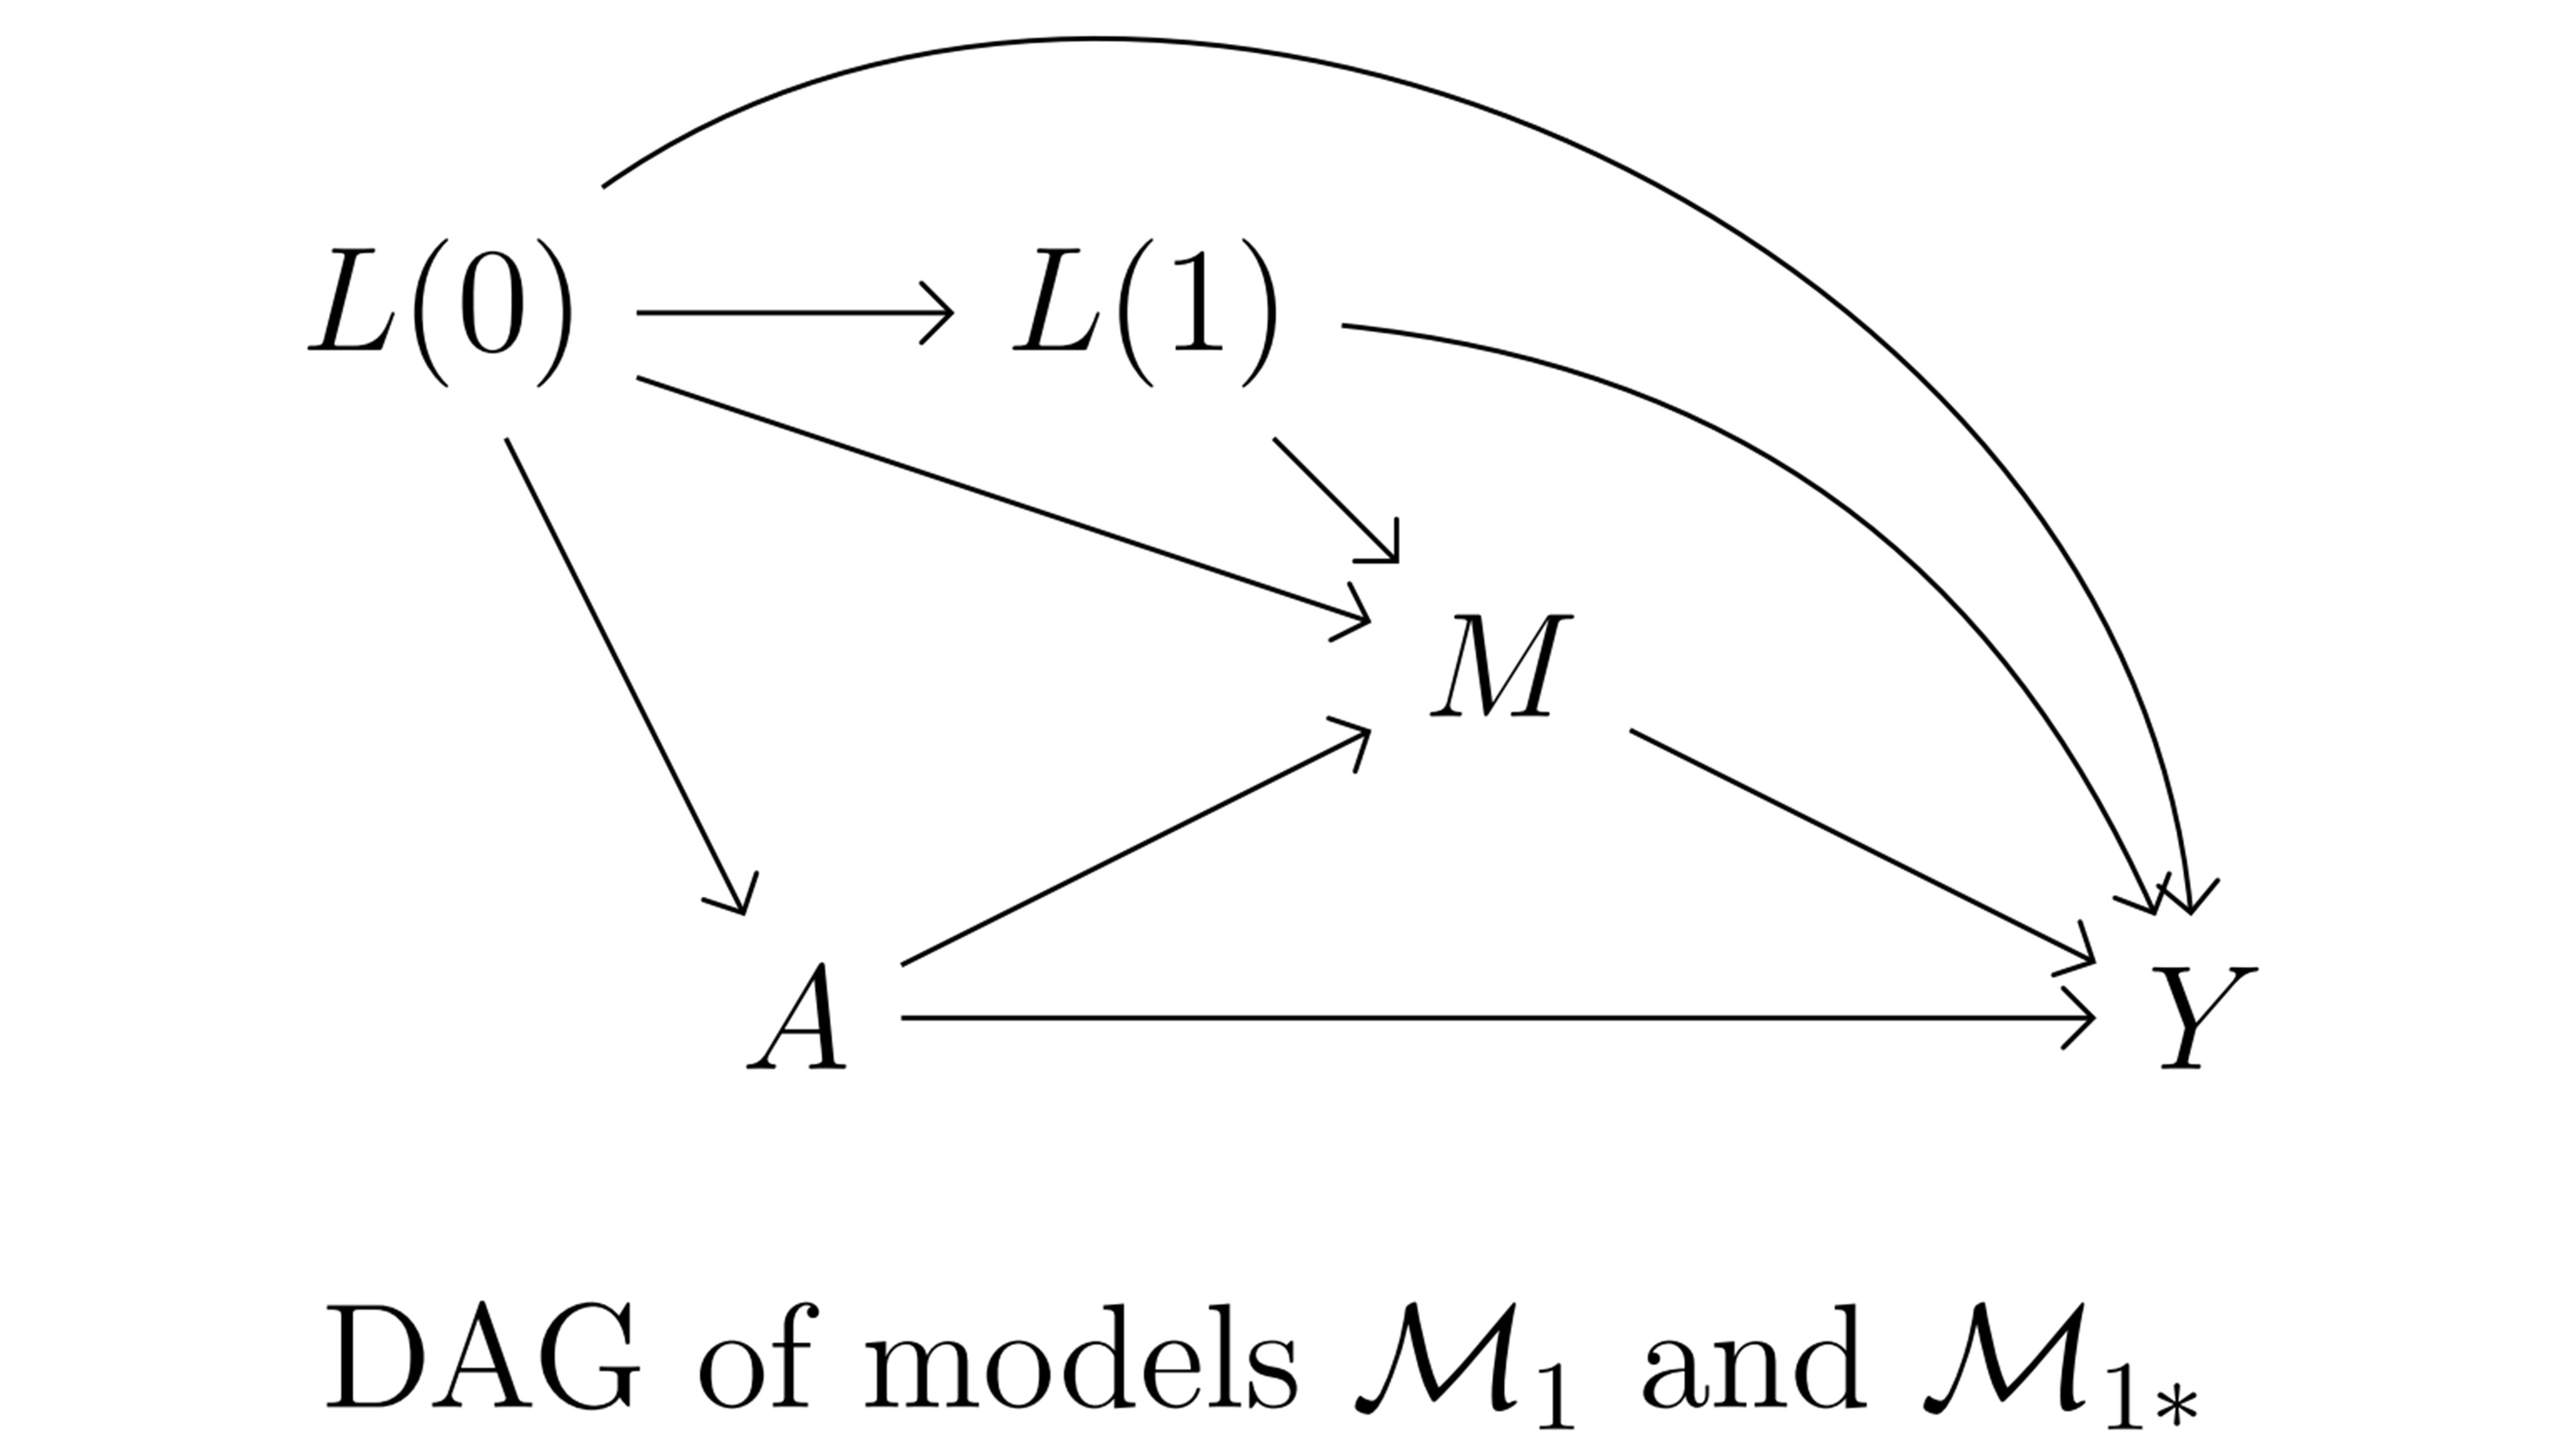
\includegraphics[width=0.5\linewidth]{./figures/DAG_M1} 

}

\caption{Causal model 1}\label{fig:figDAGM1}
\end{figure}

\begin{itemize}
\tightlist
\item
  The next two data set are simulated from a causal model where confounders of the mediator-outcome relationship (\(L(1)\)) are affected by the exposure \(A\) (Figure \ref{fig:figDAGM2}),

  \begin{itemize}
  \tightlist
  \item
    The data set \texttt{df2.csv} is simulated from the statistical model \(\mathcal{M}_2\), which does not contain any \(A \ast M\) interaction effect on the outcome \(Y\).
  \item
    The data set \texttt{df2\_int.csv} is simulated from the statistical model \(\mathcal{M}_{2 \ast}\), which contains an \(A \ast M\) interaction effect on the outcome \(Y\).
  \end{itemize}
\end{itemize}

\begin{figure}

{\centering 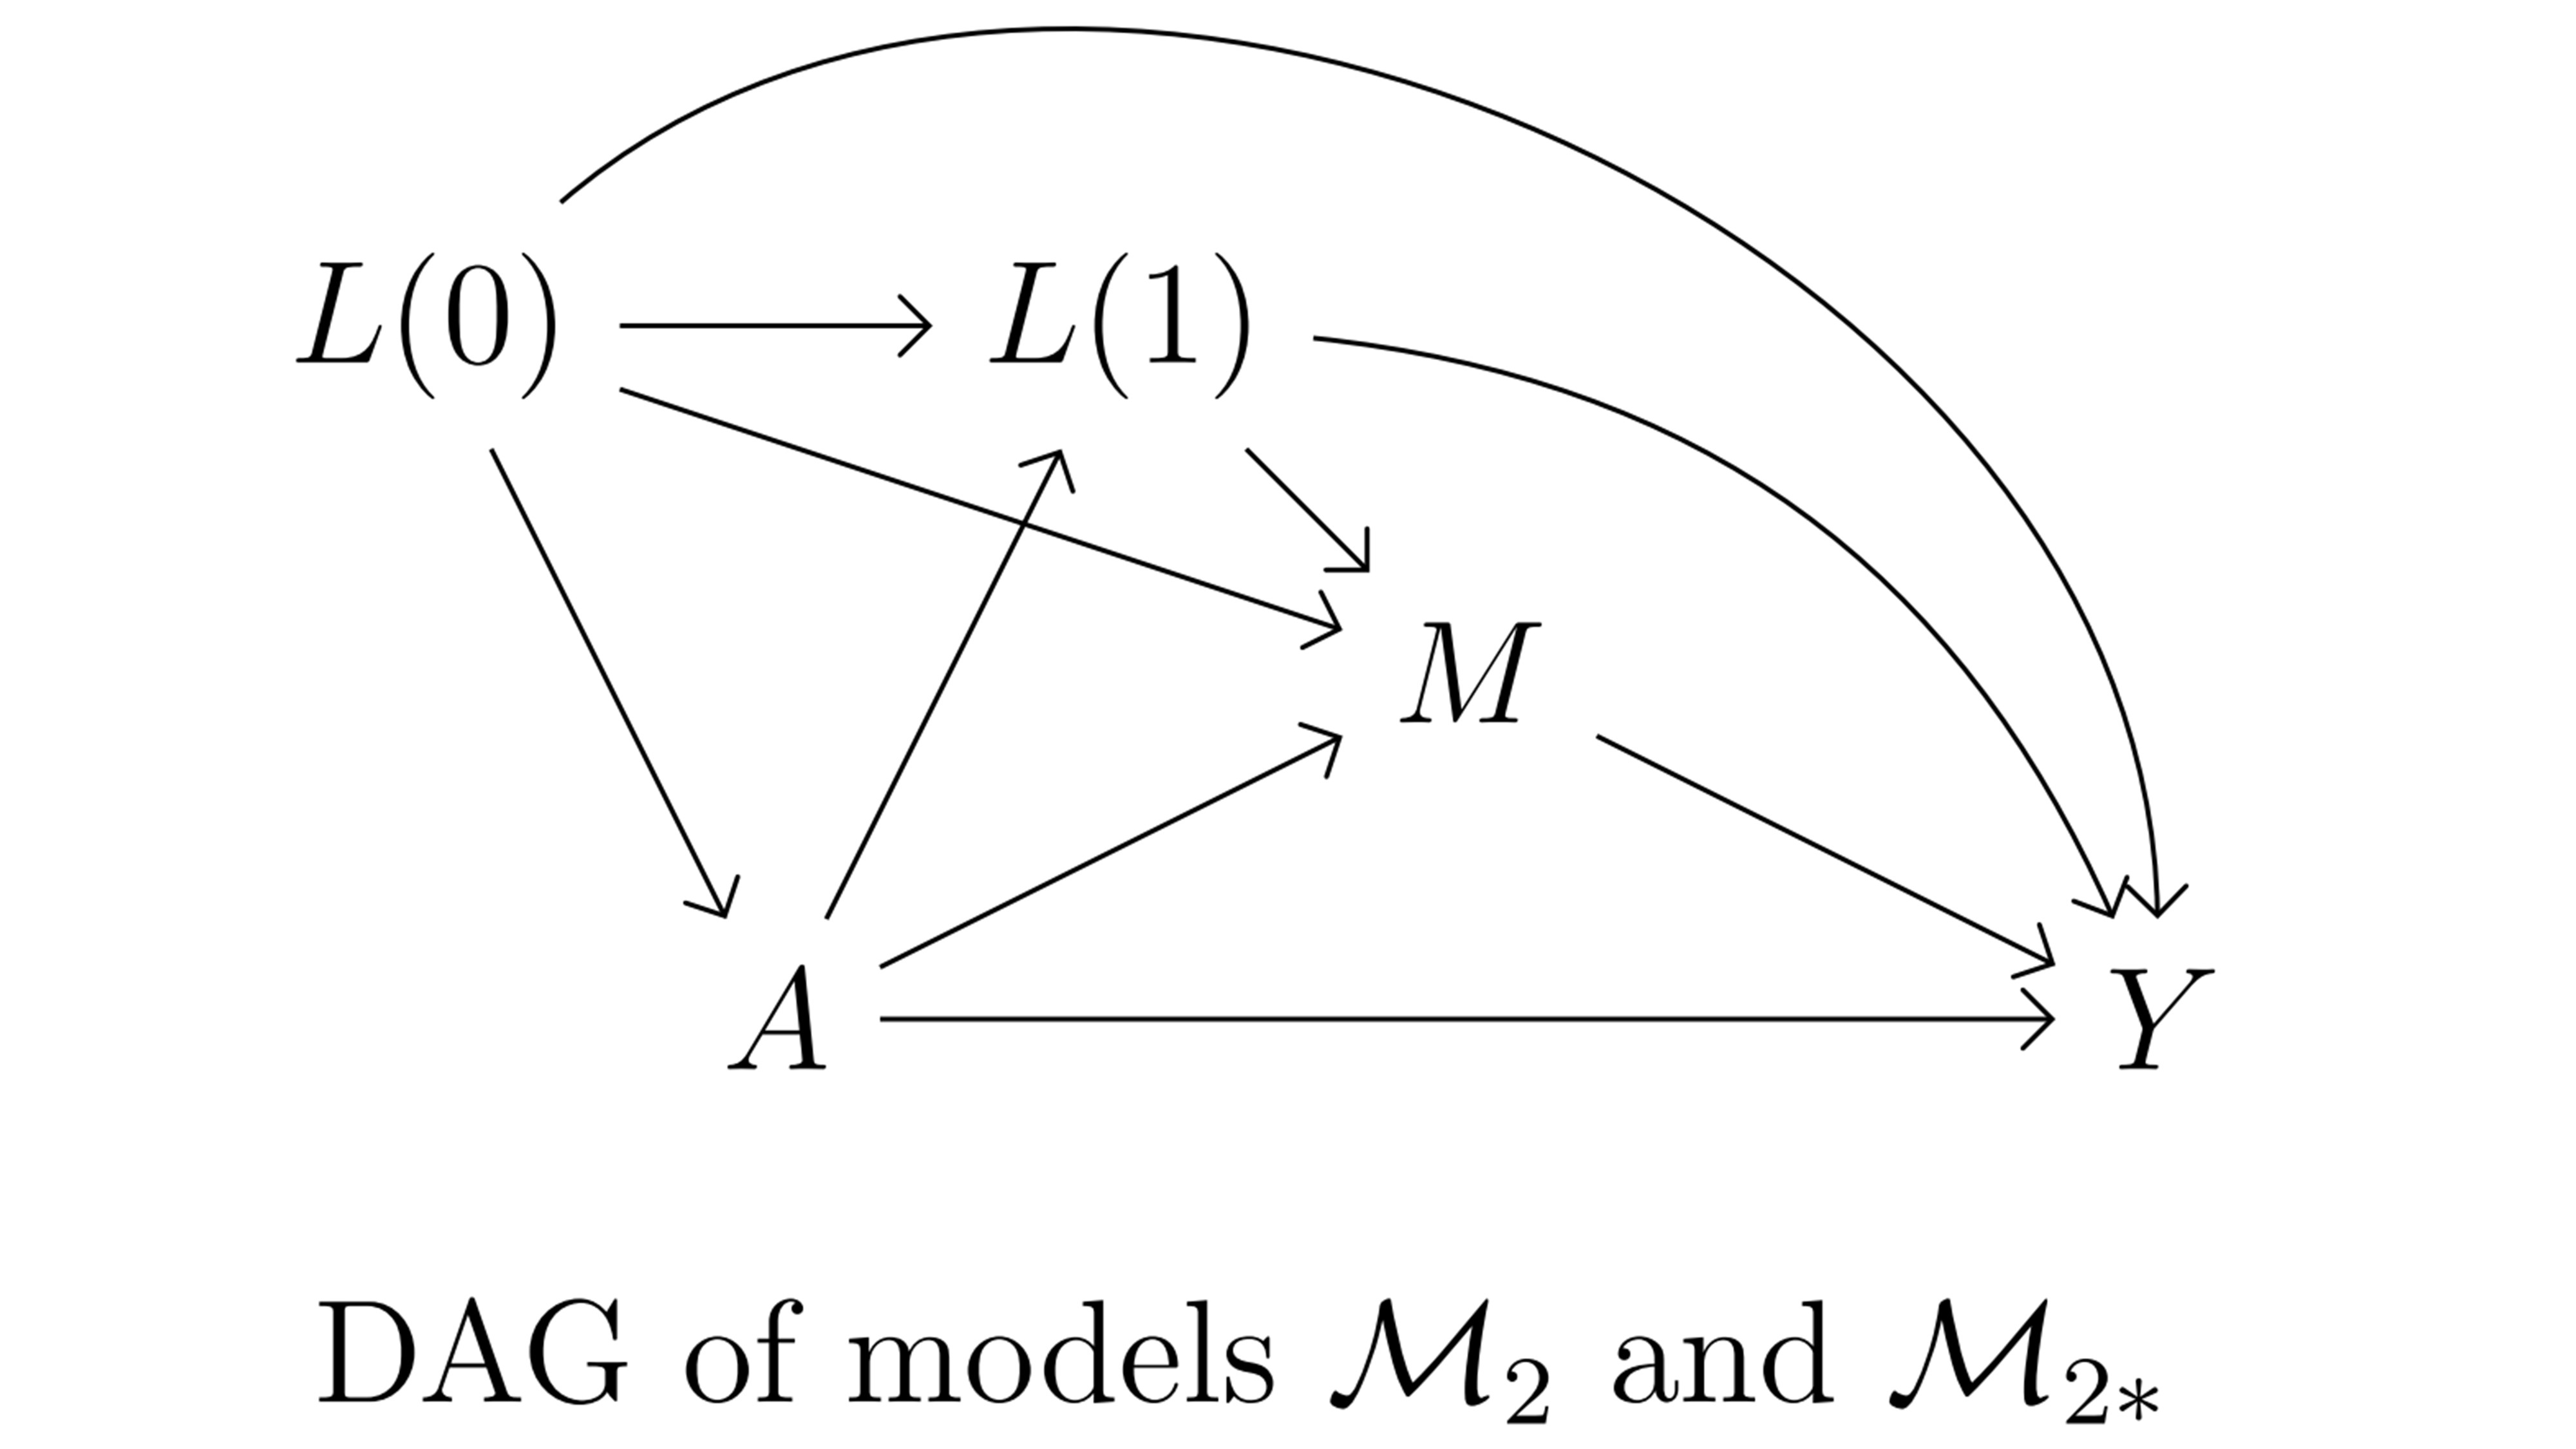
\includegraphics[width=0.5\linewidth]{./figures/DAG_M2} 

}

\caption{Causal model 2}\label{fig:figDAGM2}
\end{figure}

The R functions used to simulate these 4 data sets are given in the Appendix A.

The Appendix B describes how the true values for the estimands of the causal quantities of interest given in Table 2 of the \emph{Expanse ``Mediation analysis'' report} were calculated. Those true values are the theoretical values expected under the causal and statistical models \(\mathcal{M}_1\), \(\mathcal{M}_{1 \ast}\), \(\mathcal{M}_2\) and \(\mathcal{M}_{2 \ast}\). Estimations that will be obtained from the data sets \texttt{df1.csv}, \texttt{df1\_int.csv}, \texttt{df2.csv}, and \texttt{df2\_int.csv} will be slightly different from the true values because of sample variability.

\hypertarget{ChapBaronKennySem}{%
\chapter{Baron and Kenny, structural equation models}\label{ChapBaronKennySem}}

\hypertarget{ChapTradRegModels}{%
\chapter{Traditional regression models}\label{ChapTradRegModels}}

Traditional regression models can be applied in the absence of an intermediate confounder \(L(1)\) of the \(M-Y\) relationship affected by the exposure \(A\) (Causal model 1). They can be used for two-way, three-way and four-way decomposition of the average total effect.

In the following examples, we use the \texttt{df1\_int.csv} data set with a \(A \star M\) interaction effect on the outcome.

\begin{Shaded}
\begin{Highlighting}[]
\NormalTok{df1\_int }\OtherTok{\textless{}{-}} \FunctionTok{read.csv}\NormalTok{(}\AttributeTok{file =} \StringTok{"df1\_int.csv"}\NormalTok{)}
\end{Highlighting}
\end{Shaded}

If we assumed that there was no \(A \star M\) interaction, then the \texttt{A0\_ace:M\_smoking} interaction terms should be removed from the models below (applicable if we use the \texttt{df1.csv} data set).

\hypertarget{estimation-of-the-average-total-effect-ate}{%
\section{Estimation of the Average Total Effect (ATE)}\label{estimation-of-the-average-total-effect-ate}}

The average total effect is the difference between the mean outcome had the whole population been exposed to adverse childhood experience (ACE), compared to the mean outcome had the whole population been unexposed to ACE:
\(\text{ATE} = \mathbb{E}(Y_{A=1}) - \mathbb{E}(Y_{A=0})\).

For the quantitative outcome, the ATE of the adverse childhood experience \(A\) on the quality of life score \(Y\) can be estimated using a traditional linear regression of \texttt{Y\_qol} on \texttt{A0\_ace}, adjusted for the baseline confounders \texttt{L0\_male} and \texttt{L0\_parent\_low\_educ\_lv}.

For the binary outcome (death), we can estimate a risk difference applying a Generalized Linear Model with a Gaussian distribution and identity link, as suggested by Naimi \emph{et al} (\protect\hyperlink{ref-naimi2020}{Naimi and Whitcomb 2020}).

The regression coefficient of the exposure variable \(A\) is used to estimate the risk difference or the average difference.
\begin{equation} 
  \mathbb{E}(Y \mid A, L(0)) = \alpha_0 + \alpha_A A + \alpha_{L(0)} L(0) 
  \label{eq:regtotaleffect}
\end{equation}

\[ \hat{\Psi}_{\text{trad}}^{\text{ATE}} = \hat{\alpha}_A\]

\begin{Shaded}
\begin{Highlighting}[]
\CommentTok{\# For quantitative outcomes, apply a linear regression of Y on A (A0\_ace), }
\CommentTok{\# adjusted for the baseline confounders L(0):}
\NormalTok{trad\_ATE\_qol }\OtherTok{\textless{}{-}} \FunctionTok{lm}\NormalTok{(Y\_qol }\SpecialCharTok{\textasciitilde{}}\NormalTok{ A0\_ace }\SpecialCharTok{+}\NormalTok{ L0\_male }\SpecialCharTok{+}\NormalTok{ L0\_parent\_low\_educ\_lv,}
                   \AttributeTok{data =}\NormalTok{ df1\_int)}

\CommentTok{\# For binary outcomes, apply a GLM of Y on A with a Gaussian distribution and}
\CommentTok{\# identity link, adjusted for the baseline confounders:}
\NormalTok{trad\_ATE\_death }\OtherTok{\textless{}{-}} \FunctionTok{glm}\NormalTok{(Y\_death }\SpecialCharTok{\textasciitilde{}}\NormalTok{ A0\_ace }\SpecialCharTok{+}\NormalTok{ L0\_male }\SpecialCharTok{+}\NormalTok{ L0\_parent\_low\_educ\_lv,}
                      \AttributeTok{family =} \FunctionTok{gaussian}\NormalTok{(}\StringTok{"identity"}\NormalTok{),}
                      \AttributeTok{data =}\NormalTok{ df1\_int)}

\CommentTok{\# Use the regression coefficient of the exposure (A0\_ace) to estimate the ATE}
\NormalTok{ATE\_trad\_qol }\OtherTok{\textless{}{-}} \FunctionTok{coefficients}\NormalTok{(trad\_ATE\_qol)[}\StringTok{"A0\_ace"}\NormalTok{]}
\CommentTok{\# {-}7.210089}

\NormalTok{ATE\_trad\_death }\OtherTok{\textless{}{-}} \FunctionTok{coefficients}\NormalTok{(trad\_ATE\_death)[}\StringTok{"A0\_ace"}\NormalTok{]}
\CommentTok{\# 0.07720726}
\end{Highlighting}
\end{Shaded}

The estimation of 95\% confidence intervals could be obtained directly from the linear regression with quantitative outcomes (equation \eqref{eq:regtotaleffect}). However, using a robust (sandwich) variance estimator or applying a bootstrap procedure is recommended (\protect\hyperlink{ref-naimi2020}{Naimi and Whitcomb 2020}).

\begin{Shaded}
\begin{Highlighting}[]
\FunctionTok{library}\NormalTok{(sandwich)}

\CommentTok{\# for the Quality of Life outcome}
\NormalTok{ATE\_trad\_qol }\OtherTok{\textless{}{-}} \FunctionTok{list}\NormalTok{(}\AttributeTok{ATE =} \FunctionTok{coef}\NormalTok{(trad\_ATE\_qol)[}\StringTok{"A0\_ace"}\NormalTok{],}
                     \AttributeTok{lo =} \FunctionTok{coef}\NormalTok{(trad\_ATE\_qol)[}\StringTok{"A0\_ace"}\NormalTok{] }\SpecialCharTok{{-}} \FunctionTok{qnorm}\NormalTok{(}\FloatTok{0.975}\NormalTok{) }\SpecialCharTok{*}
                       \FunctionTok{sqrt}\NormalTok{(}\FunctionTok{sandwich}\NormalTok{(trad\_ATE\_qol)[}\StringTok{"A0\_ace"}\NormalTok{,}\StringTok{"A0\_ace"}\NormalTok{]),}
                     \AttributeTok{hi =} \FunctionTok{coef}\NormalTok{(trad\_ATE\_qol)[}\StringTok{"A0\_ace"}\NormalTok{] }\SpecialCharTok{+} \FunctionTok{qnorm}\NormalTok{(}\FloatTok{0.975}\NormalTok{) }\SpecialCharTok{*}
                       \FunctionTok{sqrt}\NormalTok{(}\FunctionTok{sandwich}\NormalTok{(trad\_ATE\_qol)[}\StringTok{"A0\_ace"}\NormalTok{,}\StringTok{"A0\_ace"}\NormalTok{]))}

\NormalTok{ATE\_trad\_qol}
\CommentTok{\# ATE = {-}7.210089 , IC95\% = [{-}7.978234 ; {-}6.441944]}

\CommentTok{\# for death outcome}
\NormalTok{ATE\_trad\_death }\OtherTok{\textless{}{-}} \FunctionTok{list}\NormalTok{(}\AttributeTok{ATE =} \FunctionTok{coef}\NormalTok{(trad\_ATE\_death)[}\StringTok{"A0\_ace"}\NormalTok{],}
                       \AttributeTok{lo =} \FunctionTok{coef}\NormalTok{(trad\_ATE\_death)[}\StringTok{"A0\_ace"}\NormalTok{] }\SpecialCharTok{{-}} \FunctionTok{qnorm}\NormalTok{(}\FloatTok{0.975}\NormalTok{) }\SpecialCharTok{*}
                         \FunctionTok{sqrt}\NormalTok{(}\FunctionTok{sandwich}\NormalTok{(trad\_ATE\_death)[}\StringTok{"A0\_ace"}\NormalTok{,}\StringTok{"A0\_ace"}\NormalTok{]),}
                       \AttributeTok{hi =} \FunctionTok{coef}\NormalTok{(trad\_ATE\_death)[}\StringTok{"A0\_ace"}\NormalTok{] }\SpecialCharTok{+} \FunctionTok{qnorm}\NormalTok{(}\FloatTok{0.975}\NormalTok{) }\SpecialCharTok{*}
                         \FunctionTok{sqrt}\NormalTok{(}\FunctionTok{sandwich}\NormalTok{(trad\_ATE\_death)[}\StringTok{"A0\_ace"}\NormalTok{,}\StringTok{"A0\_ace"}\NormalTok{]))}
\NormalTok{ATE\_trad\_death}
\CommentTok{\# ATE = 0.07720726 , IC95\% = [0.04945859 ; 0.1049559]}

\CommentTok{\# 95\% CI calculation applying a bootstrap procedure}
\FunctionTok{library}\NormalTok{(boot)}
\NormalTok{bootfunc }\OtherTok{\textless{}{-}} \ControlFlowTok{function}\NormalTok{(data,index)\{}
\NormalTok{  boot\_dat }\OtherTok{\textless{}{-}}\NormalTok{ data[index,]}
\NormalTok{  mod.qol }\OtherTok{\textless{}{-}} \FunctionTok{lm}\NormalTok{(Y\_qol }\SpecialCharTok{\textasciitilde{}}\NormalTok{ A0\_ace }\SpecialCharTok{+}\NormalTok{ L0\_male }\SpecialCharTok{+}\NormalTok{ L0\_parent\_low\_educ\_lv,}
                \AttributeTok{data =}\NormalTok{ boot\_dat)}
\NormalTok{  mod.death }\OtherTok{\textless{}{-}} \FunctionTok{glm}\NormalTok{(Y\_death }\SpecialCharTok{\textasciitilde{}}\NormalTok{ A0\_ace }\SpecialCharTok{+}\NormalTok{ L0\_male }\SpecialCharTok{+}\NormalTok{ L0\_parent\_low\_educ\_lv,}
                   \AttributeTok{family =} \FunctionTok{gaussian}\NormalTok{(}\StringTok{"identity"}\NormalTok{),}
                   \AttributeTok{data =}\NormalTok{ boot\_dat)}
\NormalTok{  est }\OtherTok{\textless{}{-}} \FunctionTok{c}\NormalTok{(}\FunctionTok{coef}\NormalTok{(mod.qol)[}\StringTok{"A0\_ace"}\NormalTok{],}
           \FunctionTok{coef}\NormalTok{(mod.death)[}\StringTok{"A0\_ace"}\NormalTok{])}
  \FunctionTok{return}\NormalTok{(est)}
\NormalTok{\}}

\FunctionTok{set.seed}\NormalTok{(}\DecValTok{1234}\NormalTok{)}
\NormalTok{boot\_est }\OtherTok{\textless{}{-}} \FunctionTok{boot}\NormalTok{(df1\_int,bootfunc,}\AttributeTok{R=}\DecValTok{2000}\NormalTok{)}

\CommentTok{\# the 95\% CI for the estimation of the ATE of ACE on QoL is:}
\FunctionTok{boot.ci}\NormalTok{(boot\_est, }\AttributeTok{index =} \DecValTok{1}\NormalTok{, }\AttributeTok{type =} \StringTok{"norm"}\NormalTok{)}
\CommentTok{\# ({-}7.978, {-}6.444 )}

\CommentTok{\# the 95\% CI for the estimation of the ATE of ACE on death is:}
\FunctionTok{boot.ci}\NormalTok{(boot\_est, }\AttributeTok{index =} \DecValTok{2}\NormalTok{, }\AttributeTok{type =} \StringTok{"norm"}\NormalTok{)}
\CommentTok{\# ( 0.0502,  0.1040 )  }
\end{Highlighting}
\end{Shaded}

Alternatively for binary outcomes, the total effect conditional on baseline confounders can be expressed on an Odds Ratio scale \(\text{OR}^{\text{TE}}\), using the logistic regression \eqref{eq:logittotaleffect}.

\begin{equation} 
  \text{logit} P(Y = 1 \mid A, L(0)) = \alpha_0 + \alpha_A A + \alpha_{L(0)}^\prime L(0) 
  \label{eq:logittotaleffect}
\end{equation}

\[ \text{OR}^{\text{TE}} \mid L(0) = \exp \hat{\alpha}_A \]

\begin{Shaded}
\begin{Highlighting}[]
\NormalTok{TE\_death\_model }\OtherTok{\textless{}{-}} \FunctionTok{glm}\NormalTok{(Y\_death }\SpecialCharTok{\textasciitilde{}}\NormalTok{ A0\_ace }\SpecialCharTok{+}\NormalTok{ L0\_male }\SpecialCharTok{+}\NormalTok{ L0\_parent\_low\_educ\_lv,}
                      \AttributeTok{family =} \StringTok{"binomial"}\NormalTok{,}
                      \AttributeTok{data =}\NormalTok{ df1\_int)}
\NormalTok{res\_TE\_death }\OtherTok{\textless{}{-}} \FunctionTok{summary}\NormalTok{(TE\_death\_model)}
\NormalTok{tot.effect.death.OR }\OtherTok{\textless{}{-}} \FunctionTok{list}\NormalTok{(}\AttributeTok{OR =} \FunctionTok{exp}\NormalTok{(}\FunctionTok{coef}\NormalTok{(res\_TE\_death)[}\StringTok{"A0\_ace"}\NormalTok{,}\StringTok{"Estimate"}\NormalTok{]),}
                            \AttributeTok{lo =} \FunctionTok{exp}\NormalTok{(}\FunctionTok{coef}\NormalTok{(res\_TE\_death)[}\StringTok{"A0\_ace"}\NormalTok{,}\StringTok{"Estimate"}\NormalTok{] }\SpecialCharTok{{-}}
                                       \FunctionTok{qnorm}\NormalTok{(}\FloatTok{0.975}\NormalTok{) }\SpecialCharTok{*}
                                       \FunctionTok{coef}\NormalTok{(res\_TE\_death)[}\StringTok{"A0\_ace"}\NormalTok{,}\StringTok{"Std. Error"}\NormalTok{]),}
                            \AttributeTok{hi =} \FunctionTok{exp}\NormalTok{(}\FunctionTok{coef}\NormalTok{(res\_TE\_death)[}\StringTok{"A0\_ace"}\NormalTok{,}\StringTok{"Estimate"}\NormalTok{] }\SpecialCharTok{+}
                                       \FunctionTok{qnorm}\NormalTok{(}\FloatTok{0.975}\NormalTok{) }\SpecialCharTok{*}
                                       \FunctionTok{coef}\NormalTok{(res\_TE\_death)[}\StringTok{"A0\_ace"}\NormalTok{,}\StringTok{"Std. Error"}\NormalTok{]))}
\NormalTok{tot.effect.death.OR}
\CommentTok{\# OR = 1.523254 , 95\% CI = [ 1.323317 ; 1.753398]}
\end{Highlighting}
\end{Shaded}

\hypertarget{trad2way}{%
\section{Two-way decomposition}\label{trad2way}}

In order to carry-out two-way decomposition mediation analyses, with a binary mediator and a continuous outcome, Valeri and VanderWeele suggest using the following linear regression of the outcome and logistic regression of the mediator:(\protect\hyperlink{ref-valeri2013}{Valeri and VanderWeele 2013})
\begin{equation}
\mathbb{E}(Y \mid A, M,L(0),L(1)) = \gamma_0 + \gamma_A A + \gamma_M M + \gamma_{A \ast M} (A \ast M) + \gamma_{L(0)}^\prime L(0) + \gamma_{L(1)}^\prime L(1) 
\label{eq:contoutcomereg}
\end{equation}

\begin{equation} 
\text{logit}P(M=1 \mid A,L(0),L(1)) = \beta_0 + \beta_A A + \beta_{L(0)}^\prime L(0) + \beta_{L(1)}^\prime L(1)
\label{eq:medreg}
\end{equation}

If the outcome is binary, they suggest using the following logistic regression of the outcome instead of the previous linear regression:
\begin{equation}
\small
\text{logit}P(Y \mid A, M,L(0),L(1)) = \gamma_0 + \gamma_A A + \gamma_M M + \gamma_{A \ast M} (A \ast M) + \gamma_{L(0)}^\prime L(0) + \gamma_{L(1)}^\prime L(1) 
\label{eq:binoutcomereg}
\end{equation}

\begin{Shaded}
\begin{Highlighting}[]
\NormalTok{trad\_qol\_am }\OtherTok{\textless{}{-}} \FunctionTok{lm}\NormalTok{(Y\_qol }\SpecialCharTok{\textasciitilde{}}\NormalTok{ A0\_ace }\SpecialCharTok{+}\NormalTok{ M\_smoking }\SpecialCharTok{+}\NormalTok{ A0\_ace}\SpecialCharTok{:}\NormalTok{M\_smoking }\SpecialCharTok{+}
\NormalTok{                    L0\_male }\SpecialCharTok{+}\NormalTok{ L0\_parent\_low\_educ\_lv }\SpecialCharTok{+}\NormalTok{ L1,}
                  \AttributeTok{data =}\NormalTok{ df1\_int)}
\NormalTok{gamma.A.q }\OtherTok{\textless{}{-}} \FunctionTok{coef}\NormalTok{(trad\_qol\_am)[}\StringTok{"A0\_ace"}\NormalTok{]}
\NormalTok{gamma.M.q }\OtherTok{\textless{}{-}} \FunctionTok{coef}\NormalTok{(trad\_qol\_am)[}\StringTok{"M\_smoking"}\NormalTok{]}
\NormalTok{gamma.AM.q }\OtherTok{\textless{}{-}} \FunctionTok{coef}\NormalTok{(trad\_qol\_am)[}\StringTok{"A0\_ace:M\_smoking"}\NormalTok{]}

\NormalTok{trad\_m }\OtherTok{\textless{}{-}} \FunctionTok{glm}\NormalTok{(M\_smoking }\SpecialCharTok{\textasciitilde{}}\NormalTok{ A0\_ace }\SpecialCharTok{+}\NormalTok{ L0\_male }\SpecialCharTok{+}\NormalTok{ L0\_parent\_low\_educ\_lv }\SpecialCharTok{+}\NormalTok{ L1, }
              \AttributeTok{family =} \StringTok{"binomial"}\NormalTok{,}
              \AttributeTok{data =}\NormalTok{ df1\_int)}
\NormalTok{beta}\FloatTok{.0} \OtherTok{\textless{}{-}} \FunctionTok{coef}\NormalTok{(trad\_m)[}\StringTok{"(Intercept)"}\NormalTok{]}
\NormalTok{beta.A }\OtherTok{\textless{}{-}} \FunctionTok{coef}\NormalTok{(trad\_m)[}\StringTok{"A0\_ace"}\NormalTok{]}

\NormalTok{trad\_death\_am }\OtherTok{\textless{}{-}} \FunctionTok{glm}\NormalTok{(Y\_death }\SpecialCharTok{\textasciitilde{}}\NormalTok{ A0\_ace }\SpecialCharTok{+}\NormalTok{ M\_smoking }\SpecialCharTok{+}\NormalTok{ A0\_ace}\SpecialCharTok{:}\NormalTok{M\_smoking }\SpecialCharTok{+}
\NormalTok{                       L0\_male }\SpecialCharTok{+}\NormalTok{ L0\_parent\_low\_educ\_lv }\SpecialCharTok{+}\NormalTok{ L1,}
                     \AttributeTok{family =} \StringTok{"binomial"}\NormalTok{,}
                     \AttributeTok{data =}\NormalTok{ df1\_int)}
\NormalTok{gamma.A.d }\OtherTok{\textless{}{-}} \FunctionTok{coef}\NormalTok{(trad\_death\_am)[}\StringTok{"A0\_ace"}\NormalTok{]}
\NormalTok{gamma.M.d }\OtherTok{\textless{}{-}} \FunctionTok{coef}\NormalTok{(trad\_death\_am)[}\StringTok{"M\_smoking"}\NormalTok{]}
\NormalTok{gamma.AM.d }\OtherTok{\textless{}{-}} \FunctionTok{coef}\NormalTok{(trad\_death\_am)[}\StringTok{"A0\_ace:M\_smoking"}\NormalTok{]}
\end{Highlighting}
\end{Shaded}

\hypertarget{trad2waycde}{%
\subsection{Controlled Direct Effect}\label{trad2waycde}}

The Controlled Direct Effect is defined as \(\text{CDE}_m = \mathbb{E}(Y_{A=1,M=m}) - \mathbb{E}(Y_{A=0,M=m})\):

For continuous outcome, using parameters from equation \eqref{eq:contoutcomereg}, it can be estimated by:
\[\text{CDE}_m = \hat{\gamma}_A + \hat{\gamma}_{A \ast M} \times m\]

\begin{Shaded}
\begin{Highlighting}[]
\DocumentationTok{\#\#\# For a continuous outcome}
\CommentTok{\# setting the mediator to M=0}
\NormalTok{trad\_CDE\_qol\_m0 }\OtherTok{\textless{}{-}}\NormalTok{ gamma.A.q }\SpecialCharTok{+}\NormalTok{ gamma.AM.q }\SpecialCharTok{*} \DecValTok{0}
\NormalTok{trad\_CDE\_qol\_m0}
\CommentTok{\# {-}3.715265}
\CommentTok{\# setting the mediator to M=1}
\NormalTok{trad\_CDE\_qol\_m1 }\OtherTok{\textless{}{-}}\NormalTok{ gamma.A.q }\SpecialCharTok{+}\NormalTok{ gamma.AM.q }\SpecialCharTok{*} \DecValTok{1}
\NormalTok{trad\_CDE\_qol\_m1}
\CommentTok{\# {-}9.330657}
\end{Highlighting}
\end{Shaded}

For binary outcomes, using parameters from equation \eqref{eq:binoutcomereg}, it can be estimated on the OR scale by:
\[OR^{\text{CDE}_m} = \text{exp}\left(\hat{\gamma}_A + \hat{\gamma}_{A \ast M} \times m\right)\]

\begin{Shaded}
\begin{Highlighting}[]
\DocumentationTok{\#\#\# For a binary outcome}
\DocumentationTok{\#\# setting the mediator to M=0}
\NormalTok{trad\_OD\_CDE\_death\_m0 }\OtherTok{\textless{}{-}} \FunctionTok{exp}\NormalTok{(gamma.A.d }\SpecialCharTok{+}\NormalTok{ gamma.AM.d }\SpecialCharTok{*} \DecValTok{0}\NormalTok{)}
\NormalTok{trad\_OD\_CDE\_death\_m0}
\CommentTok{\# OR\_CDE\_\{M=0\} = 1.442942 }

\DocumentationTok{\#\# setting the mediator to M=1}
\NormalTok{trad\_OD\_CDE\_death\_m1 }\OtherTok{\textless{}{-}} \FunctionTok{exp}\NormalTok{(gamma.A.d }\SpecialCharTok{+}\NormalTok{ gamma.AM.d }\SpecialCharTok{*} \DecValTok{1}\NormalTok{)}
\NormalTok{trad\_OD\_CDE\_death\_m1}
\CommentTok{\# OR\_CDE\_\{M=1\} = 1.461464 }
\end{Highlighting}
\end{Shaded}

\hypertarget{trad2waynatural}{%
\subsection{Natural Direct and Indirect effects}\label{trad2waynatural}}

The Pure Natural Direct Effect (PNDE) and the Total Natural Indirect Effect (TNIE) are defined as:

\begin{itemize}
\tightlist
\item
  \(\text{PNDE} = \mathbb{E}\left(Y_{A=1,M_{A=0}}) - \mathbb{E}(Y_{A=0,M_{A=0}}\right)\),
\item
  \(\text{TNIE} = \mathbb{E}\left(Y_{A=1,M_{A=1}}) - \mathbb{E}(Y_{A=1,M_{A=0}}\right)\).
\end{itemize}

Alternatively, one can use the Total Natural Direct Effect (TNDE) and the Pure Natural Indirect Effect (PNIE):

\begin{itemize}
\tightlist
\item
  \(\text{TNDE} = \mathbb{E}\left(Y_{A=1,M_{A=1}}) - \mathbb{E}(Y_{A=0,M_{A=1}}\right)\),
\item
  \(\text{PNIE} = \mathbb{E}\left(Y_{A=0,M_{A=1}}) - \mathbb{E}(Y_{A=0,M_{A=0}}\right)\).
\end{itemize}

With a continuous outcome and a binary mediator, the PNDE and TNDE can be estimated using the linear regression of the outcome (equation \eqref{eq:contoutcomereg}) and the logistic regression of the mediator (equation \eqref{eq:medreg}):
\[\text{PNDE} \mid L(0), L(1) = \hat{\gamma}_A + \hat{\gamma}_{A \ast M} \frac{exp(\hat{\beta}_0 + \hat{\beta}_A \times 0 + \hat{\beta}_{L(0)}^\prime L(0) + \hat{\beta}_{L(1)}^\prime L(1))}{1 + exp(\hat{\beta}_0 + \hat{\beta}_A \times 0 + \hat{\beta}_{L(0)}^\prime L(0) + \hat{\beta}_{L(1)}^\prime L(1))}\]

\[\scriptsize
\text{TNIE} \mid L(0), L(1) = \left( \hat{\gamma}_M + \hat{\gamma}_{A \ast M} \times 1 \right) \left[ \frac{exp(\hat{\beta}_0 + \hat{\beta}_A \times 1 + \hat{\beta}_{L(0)}^\prime L(0) + \hat{\beta}_{L(1)}^\prime L(1))}{1 + exp(\hat{\beta}_0 + \hat{\beta}_A \times 1 + \hat{\beta}_{L(0)}^\prime L(0) + \hat{\beta}_{L(1)}^\prime L(1))} - \frac{exp(\hat{\beta}_0 + \hat{\beta}_A \times 0 + \hat{\beta}_{L(0)}^\prime L(0) + \hat{\beta}_{L(1)}^\prime L(1))}{1 + exp(\hat{\beta}_0 + \hat{\beta}_A \times 0 + \hat{\beta}_{L(0)}^\prime L(0) + \hat{\beta}_{L(1)}^\prime L(1))}\right]\]
The alternative TNDE ad PNIE can be estimated by:
\[\text{TNDE} \mid L(0), L(1) = \hat{\gamma}_A + \hat{\gamma}_{A \ast M}\frac{exp(\hat{\beta}_0 + \hat{\beta}_A \times 1 + \hat{\beta}_{L(0)}^\prime L(0) + \hat{\beta}_{L(1)}^\prime L(1))}{1 + exp(\hat{\beta}_0 + \hat{\beta}_A \times 1 + \hat{\beta}_{L(0)}^\prime L(0) + \hat{\beta}_{L(1)}^\prime L(1))}\]
\[\scriptsize \text{PNIE} \mid L(0), L(1) = \left( \hat{\gamma}_M + \hat{\gamma}_{A \ast M} \times 0 \right) \left[ \frac{exp(\hat{\beta}_0 + \hat{\beta}_A \times 1 + \hat{\beta}_{L(0)}^\prime L(0) + \hat{\beta}_{L(1)}^\prime L(1))}{1 + exp(\hat{\beta}_0 + \hat{\beta}_A \times 1 + \hat{\beta}_{L(0)}^\prime L(0) + \hat{\beta}_{L(1)}^\prime L(1))} - \frac{exp(\hat{\beta}_0 + \hat{\beta}_A \times 0 + \hat{\beta}_{L(0)}^\prime L(0) + \hat{\beta}_{L(1)}^\prime L(1))}{1 + exp(\hat{\beta}_0 + \hat{\beta}_A \times 0 + \hat{\beta}_{L(0)}^\prime L(0) + \hat{\beta}_{L(1)}^\prime L(1))}\right]\]
Conditional on participants for which \(L(0)=0\) and \(L(1)=0\), these expressions are simplified:
\[\text{PNDE} \Big| (L(0)=0, L(1)=0) = \hat{\gamma}_A + \hat{\gamma}_{A \ast M}\frac{exp(\hat{\beta}_0)}{1 + exp(\hat{\beta}_0)}\]
\[\text{TNIE} \Big| (L(0)=0, L(1)=0) = \left( \hat{\gamma}_M + \hat{\gamma}_{A \ast M} \right) \left[ \frac{exp(\hat{\beta}_0 + \hat{\beta}_A )}{1 + exp(\hat{\beta}_0 + \hat{\beta}_A )} - \frac{exp(\hat{\beta}_0 )}{1 + exp(\hat{\beta}_0)}\right]\]
and
\[\text{TNDE} \Big| (L(0)=0, L(1)=0) = \hat{\gamma}_A + \hat{\gamma}_{A \ast M}\frac{exp(\hat{\beta}_0 + \hat{\beta}_A)}{1 + exp(\hat{\beta}_0 + \hat{\beta}_A)}\]
\[\text{PNIE} \Big| (L(0)=0, L(1)=0) = \hat{\gamma}_M \left[ \frac{exp(\hat{\beta}_0 + \hat{\beta}_A )}{1 + exp(\hat{\beta}_0 + \hat{\beta}_A )} - \frac{exp(\hat{\beta}_0 )}{1 + exp(\hat{\beta}_0)}\right]\]

\begin{Shaded}
\begin{Highlighting}[]
\DocumentationTok{\#\#\# For a continuous outcome, in the subgroup with L(0)=0 and L(1)=0}
\DocumentationTok{\#\# The PNDE and TNIE are:}
\NormalTok{trad\_PNDE\_qol }\OtherTok{\textless{}{-}}\NormalTok{ gamma.A.q }\SpecialCharTok{+}\NormalTok{ gamma.AM.q }\SpecialCharTok{*}\NormalTok{ (}\FunctionTok{exp}\NormalTok{(beta}\FloatTok{.0}\NormalTok{)) }\SpecialCharTok{/}\NormalTok{ (}\DecValTok{1} \SpecialCharTok{+} \FunctionTok{exp}\NormalTok{(beta}\FloatTok{.0}\NormalTok{))}
\NormalTok{trad\_PNDE\_qol}
\CommentTok{\# {-}4.845089}

\NormalTok{trad\_TNIE\_qol }\OtherTok{\textless{}{-}}\NormalTok{ (gamma.M.q }\SpecialCharTok{+}\NormalTok{ gamma.AM.q) }\SpecialCharTok{*}
\NormalTok{  (}\FunctionTok{exp}\NormalTok{(beta}\FloatTok{.0} \SpecialCharTok{+}\NormalTok{ beta.A) }\SpecialCharTok{/}\NormalTok{ (}\DecValTok{1} \SpecialCharTok{+} \FunctionTok{exp}\NormalTok{(beta}\FloatTok{.0} \SpecialCharTok{+}\NormalTok{ beta.A)) }\SpecialCharTok{{-}}
     \FunctionTok{exp}\NormalTok{(beta}\FloatTok{.0}\NormalTok{) }\SpecialCharTok{/}\NormalTok{ (}\DecValTok{1} \SpecialCharTok{+} \FunctionTok{exp}\NormalTok{(beta}\FloatTok{.0}\NormalTok{)))}
\NormalTok{trad\_TNIE\_qol}
\CommentTok{\# {-}1.50119}

\DocumentationTok{\#\# The TNDE and PNIE are:}
\NormalTok{trad\_TNDE\_qol }\OtherTok{\textless{}{-}}\NormalTok{ gamma.A.q }\SpecialCharTok{+}
\NormalTok{  gamma.AM.q }\SpecialCharTok{*} \FunctionTok{exp}\NormalTok{(beta}\FloatTok{.0} \SpecialCharTok{+}\NormalTok{ beta.A) }\SpecialCharTok{/}\NormalTok{ (}\DecValTok{1} \SpecialCharTok{+} \FunctionTok{exp}\NormalTok{(beta}\FloatTok{.0} \SpecialCharTok{+}\NormalTok{ beta.A))}
\NormalTok{trad\_TNDE\_qol}
\CommentTok{\# {-}5.436773}

\NormalTok{trad\_PNIE\_qol }\OtherTok{\textless{}{-}}\NormalTok{ gamma.M.q }\SpecialCharTok{*}
\NormalTok{  (}\FunctionTok{exp}\NormalTok{(beta}\FloatTok{.0} \SpecialCharTok{+}\NormalTok{ beta.A) }\SpecialCharTok{/}
\NormalTok{     (}\DecValTok{1} \SpecialCharTok{+} \FunctionTok{exp}\NormalTok{(beta}\FloatTok{.0} \SpecialCharTok{+}\NormalTok{ beta.A)) }\SpecialCharTok{{-}} \FunctionTok{exp}\NormalTok{(beta}\FloatTok{.0}\NormalTok{) }\SpecialCharTok{/}\NormalTok{ (}\DecValTok{1} \SpecialCharTok{+} \FunctionTok{exp}\NormalTok{(beta}\FloatTok{.0}\NormalTok{)))}
\NormalTok{trad\_PNIE\_qol}
\CommentTok{\# {-}0.9095061}
\end{Highlighting}
\end{Shaded}

\textbf{For binary outcomes}, total, direct and indirect effects can be expressed on relative risk or odds ratio scales:

The total effect risk ratio is equal to :
\[\text{RR}^\text{TE}=\frac{\mathbb{E}(Y_1)}{\mathbb{E}(Y_0)}=\frac{\mathbb{E}(Y_{1,M_1})}{\mathbb{E}(Y_{0,M_0})}\]

The total effect risk ratio can be decomposed as the product of the PNDE risk ratio and the TNIE risk ratio:
\[\text{RR}^\text{TE}=\frac{\mathbb{E}(Y_{1,M_1})}{\mathbb{E}(Y_{0,M_0})}=\frac{\mathbb{E}(Y_{1,M_0})}{\mathbb{E}(Y_{0,M_0})} \times \frac{\mathbb{E}(Y_{1,M_1})}{\mathbb{E}(Y_{1,M_0})}=\text{RR}^\text{PNDE} \times \text{RR}^\text{TNIE}\]

Similarly, the total effect risk ratio can be decomposed as the product of the TNDE risk ratio and the PNIE risk ratio:
\[\text{RR}^\text{TE}=\frac{\mathbb{E}(Y_{1,M_1})}{\mathbb{E}(Y_{0,M_0})}=\frac{\mathbb{E}(Y_{1,M_1})}{\mathbb{E}(Y_{0,M_1})} \times \frac{\mathbb{E}(Y_{0,M_1})}{\mathbb{E}(Y_{0,M_0})}=\text{RR}^\text{TNDE} \times \text{RR}^\text{PNIE}\]

PNDE, TNIE, TNDE and PNIE can also be given on the OR scale,
\[\text{OR}^\text{PNDE} = \frac{\frac{P\left(Y_{A=1,M_{A=0}}=1\right)}{1 - P\left(Y_{A=1,M_{A=0}}=1\right)}}{\frac{P\left(Y_{A=0,M_{A=0}}=1\right)}{1 - P\left(Y_{A=0,M_{A=0}}=1\right)}} \quad \text{,} \quad \text{OR}^\text{TNIE} = \frac{\frac{P\left(Y_{A=1,M_{A=1}}=1\right)}{1 - P\left(Y_{A=1,M_{A=1}}=1\right)}}{\frac{P\left(Y_{A=1,M_{A=0}}=1\right)}{1 - P\left(Y_{A=1,M_{A=0}}=1\right)}}\]
and
\[\text{OR}^\text{TNDE} = \frac{\frac{P\left(Y_{A=1,M_{A=0}}=1\right)}{1 - P\left(Y_{A=1,M_{A=0}}=1\right)}}{\frac{P\left(Y_{A=0,M_{A=0}}=1\right)}{1 - P\left(Y_{A=0,M_{A=0}}=1\right)}} \quad \text{and} \quad \text{OR}^\text{PNIE} = \frac{\frac{P\left(Y_{A=1,M_{A=1}}=1\right)}{1 - P\left(Y_{A=1,M_{A=1}}=1\right)}}{\frac{P\left(Y_{A=1,M_{A=0}}=1\right)}{1 - P\left(Y_{A=1,M_{A=0}}=1\right)}}.\]
If the outcome is rare, we have \(P(Y=1) \approx \frac{P(Y=1)}{1-P(Y=1)}\) so that, \(\text{OR}^{\text{PNDE}}\) AND \(\text{OR}^{\text{TNIE}}\) can be estimated using the logistic model of the outcome (equation \eqref{eq:binoutcomereg}) and the logistic model of the mediator (equation \eqref{eq:medreg}):
\[\small \text{OR}^\text{PNDE} \mid L(0), L(1) \approx \frac{\text{exp}(\hat{\gamma}_A \times 1) \left[ 1 + \text{exp}(\hat{\gamma}_M + \hat{\gamma}_{A \ast M} \times 1 + \hat{\beta}_0  + \hat{\beta}_A \times 0 + \hat{\beta}_{L(0)}^\prime L(0) + \hat{\beta}_{L(1)}^\prime L(1))\right]}{ \text{exp}(\hat{\gamma}_A \times 0) \left[ 1 + \text{exp}(\hat{\gamma}_M + \hat{\gamma}_{A \ast M} \times 0 + \hat{\beta}_0 + \hat{\beta}_A \times 0  + \hat{\beta}_{L(0)}^\prime L(0) + \hat{\beta}_{L(1)}^\prime L(1))\right]} \]

and

\[ \scriptsize \text{OR}^\text{TNIE} \mid L(0), L(1) \approx \frac{\left[1 + \text{exp}(\hat{\beta}_0 + \hat{\beta}_A \times 0 + \hat{\beta}_{L(0)}^\prime L(0) + \hat{\beta}_{L(1)}^\prime L(1)) \right]  \left[ 1 + \text{exp}(\hat{\gamma}_M + \hat{\gamma}_{A \ast M} \times 1 + \hat{\beta}_0  + \hat{\beta}_A \times 1 + \hat{\beta}_{L(0)}^\prime L(0) + \hat{\beta}_{L(1)}^\prime L(1))\right]}{ \left[1 + \text{exp}(\hat{\beta}_0  + \hat{\beta}_A \times 1 + \hat{\beta}_{L(0)}^\prime L(0) + \hat{\beta}_{L(1)}^\prime L(1)) \right]  \left[ 1 + \text{exp}(\hat{\gamma}_M + \hat{\gamma}_{A \ast M} \times 1 + \hat{\beta}_0 + \hat{\beta}_A \times 0 + \hat{\beta}_{L(0)}^\prime L(0) + \hat{\beta}_{L(1)}^\prime L(1))\right]} \]
Similarly, if the outcome is rare, \(\text{OR}^{\text{TNDE}}\) AND \(\text{OR}^{\text{PNIE}}\) can be estimated using the logistic regression models for the outcome and the mediator (equations \eqref{eq:binoutcomereg} and \eqref{eq:medreg}):
\[\small \text{OR}^\text{TNDE} \mid L(0), L(1) \approx \frac{\text{exp}\left(\hat{\gamma}_A \times 1 \right)  \left[ 1 + \text{exp}\left(\hat{\gamma}_M + \hat{\gamma}_{A \ast M} \times 1 + \hat{\beta}_0 + \hat{\beta}_A \times 1 + \hat{\beta}_{L(0)}^\prime L(0) + \hat{\beta}_{L(1)}^\prime L(1)\right)\right]}{ \text{exp}\left(\hat{\gamma}_A \times 0 \right) \left[ 1 + \text{exp}\left(\hat{\gamma}_M + \hat{\gamma}_{A \ast M} \times 0 + \hat{\beta}_0 + \hat{\beta}_A \times 1 + \hat{\beta}_{L(0)}^\prime L(0) + \hat{\beta}_{L(1)}^\prime L(1)\right)\right]}\]

and
\[\scriptsize \text{OR}^\text{PNIE} \mid L(0), L(1) \approx \frac{\left[1 + \text{exp}\left(\hat{\beta}_0  + \hat{\beta}_A \times 0 + \hat{\beta}_{L(0)}^\prime L(0) + \hat{\beta}_{L(1)}^\prime L(1)\right) \right] \left[ 1 + \text{exp}\left(\hat{\gamma}_M + \hat{\gamma}_{A \ast M} \times 0 + \hat{\beta}_0  + \hat{\beta}_A \times 1 + \hat{\beta}_{L(0)}^\prime L(0) + \hat{\beta}_{L(1)}^\prime L(1)\right)\right]}{ \left[1 + \text{exp}\left(\hat{\beta}_0  + \hat{\beta}_A \times 1 + \hat{\beta}_{L(0)}^\prime L(0) + \hat{\beta}_{L(1)}^\prime L(1)\right) \right] \left[ 1 + \text{exp}\left(\hat{\gamma}_M + \hat{\gamma}_{A \ast M} \times 0 + \hat{\beta}_0 + \hat{\beta}_A \times 0 + \hat{\beta}_{L(0)}^\prime L(0) + \hat{\beta}_{L(1)}^\prime L(1)\right)\right]} \]
Conditional on participants for which \(L(0)=0\) and \(L(1)=0\), these expressions are simplified:
\[\text{OR}^\text{PNDE} \Bigg| \left(L(0) = 0, L(1) = 0\right) \approx \frac{\text{exp}\left(\hat{\gamma}_A\right) \left[ 1 + \text{exp}\left(\hat{\gamma}_M + \hat{\gamma}_{A \ast M} + \hat{\beta}_0\right)\right]}{ \left[ 1 + \text{exp}\left(\hat{\gamma}_M + \hat{\beta}_0 \right)\right]}\]
and
\[\text{OR}^\text{TNIE} \Bigg| \left(L(0)=0, L(1)=0\right) \approx \frac{\left[1 + \text{exp}\left(\hat{\beta}_0\right) \right] \times \left[ 1 + \text{exp}\left(\hat{\gamma}_M + \hat{\gamma}_{A \ast M} + \hat{\beta}_0  + \hat{\beta}_A\right)\right]}{ \left[1 + \text{exp}\left(\hat{\beta}_0  + \hat{\beta}_A \right) \right] \times \left[ 1 + \text{exp}\left(\hat{\gamma}_M + \hat{\gamma}_{A \ast M} + \hat{\beta}_0 \right)\right]} \]
Similarly, conditional on \(L(0)=0\) and \(L(1)=0\),
\[\text{OR}^\text{TNDE} \Bigg| \left(L(0)=0, L(1)=0\right) \approx \frac{\text{exp}\left(\hat{\gamma}_A\right) \left[ 1 + \text{exp}\left(\hat{\gamma}_M + \hat{\gamma}_{A \ast M} + \hat{\beta}_0 + \hat{\beta}_A \right)\right]}{ \left[ 1 + \text{exp}\left(\hat{\gamma}_M + \hat{\beta}_0 + \hat{\beta}_A \right)\right]}\]
\[\text{OR}^\text{PNIE} \Bigg| \left(L(0)=0, L(1)=0\right) \approx \frac{\left[1 + \text{exp}\left(\hat{\beta}_0 \right) \right] \times \left[ 1 + \text{exp}\left(\hat{\gamma}_M + \hat{\beta}_0  + \hat{\beta}_A \right)\right]}{ \left[1 + \text{exp}\left(\hat{\beta}_0  + \hat{\beta}_A \right) \right] \times \left[ 1 + \text{exp}\left(\hat{\gamma}_M +  \hat{\beta}_0 \right)\right]} \]

\begin{Shaded}
\begin{Highlighting}[]
\DocumentationTok{\#\#\# For a binary outcome, in the subgroup with L(0)=0 and L(1)=0}
\DocumentationTok{\#\# The PNDE and TNIE are (on the OR scale):}
\NormalTok{trad\_OR\_PNDE\_death }\OtherTok{\textless{}{-}} \FunctionTok{exp}\NormalTok{(gamma.A.d) }\SpecialCharTok{*}
\NormalTok{  (}\DecValTok{1} \SpecialCharTok{+} \FunctionTok{exp}\NormalTok{(gamma.M.d }\SpecialCharTok{+}\NormalTok{ gamma.AM.d }\SpecialCharTok{+}\NormalTok{ beta}\FloatTok{.0}\NormalTok{ )) }\SpecialCharTok{/}
\NormalTok{  (}\DecValTok{1} \SpecialCharTok{+} \FunctionTok{exp}\NormalTok{(gamma.M.d }\SpecialCharTok{+}\NormalTok{ beta}\FloatTok{.0}\NormalTok{))}
\NormalTok{trad\_OR\_PNDE\_death}
\CommentTok{\# 1.448035}

\NormalTok{trad\_OR\_TNIE\_death }\OtherTok{\textless{}{-}}\NormalTok{ (}\DecValTok{1} \SpecialCharTok{+} \FunctionTok{exp}\NormalTok{(beta}\FloatTok{.0}\NormalTok{)) }\SpecialCharTok{*}
\NormalTok{  (}\DecValTok{1} \SpecialCharTok{+} \FunctionTok{exp}\NormalTok{(gamma.M.d }\SpecialCharTok{+}\NormalTok{ gamma.AM.d }\SpecialCharTok{+}\NormalTok{ beta}\FloatTok{.0} \SpecialCharTok{+}\NormalTok{ beta.A)) }\SpecialCharTok{/}
\NormalTok{  ((}\DecValTok{1} \SpecialCharTok{+} \FunctionTok{exp}\NormalTok{(beta}\FloatTok{.0} \SpecialCharTok{+}\NormalTok{ beta.A)) }\SpecialCharTok{*}\NormalTok{ (}\DecValTok{1} \SpecialCharTok{+} \FunctionTok{exp}\NormalTok{(gamma.M.d }\SpecialCharTok{+}\NormalTok{ gamma.AM.d }\SpecialCharTok{+}\NormalTok{ beta}\FloatTok{.0}\NormalTok{)))}
\NormalTok{trad\_OR\_TNIE\_death}
\CommentTok{\# 1.050029}

\DocumentationTok{\#\# The TNDE and PNIE are (on the OR scale):}
\NormalTok{trad\_OR\_TNDE\_death }\OtherTok{\textless{}{-}} \FunctionTok{exp}\NormalTok{(gamma.A.d) }\SpecialCharTok{*}
\NormalTok{  (}\DecValTok{1} \SpecialCharTok{+} \FunctionTok{exp}\NormalTok{(gamma.M.d }\SpecialCharTok{+}\NormalTok{ gamma.AM.d }\SpecialCharTok{+}\NormalTok{ beta}\FloatTok{.0} \SpecialCharTok{+}\NormalTok{ beta.A)) }\SpecialCharTok{/}
\NormalTok{  (}\DecValTok{1} \SpecialCharTok{+} \FunctionTok{exp}\NormalTok{(gamma.M.d }\SpecialCharTok{+}\NormalTok{ beta}\FloatTok{.0} \SpecialCharTok{+}\NormalTok{ beta.A))}
\NormalTok{trad\_OR\_TNDE\_death}
\CommentTok{\# 1.450344}

\NormalTok{trad\_OR\_PNIE\_death }\OtherTok{\textless{}{-}}\NormalTok{ (}\DecValTok{1} \SpecialCharTok{+} \FunctionTok{exp}\NormalTok{(beta}\FloatTok{.0}\NormalTok{)) }\SpecialCharTok{*}
\NormalTok{  (}\DecValTok{1} \SpecialCharTok{+} \FunctionTok{exp}\NormalTok{(gamma.M.d }\SpecialCharTok{+}\NormalTok{ beta}\FloatTok{.0} \SpecialCharTok{+}\NormalTok{ beta.A)) }\SpecialCharTok{/}
\NormalTok{  ((}\DecValTok{1} \SpecialCharTok{+} \FunctionTok{exp}\NormalTok{(beta}\FloatTok{.0} \SpecialCharTok{+}\NormalTok{ beta.A)) }\SpecialCharTok{*}\NormalTok{ (}\DecValTok{1} \SpecialCharTok{+} \FunctionTok{exp}\NormalTok{(gamma.M.d }\SpecialCharTok{+}\NormalTok{ beta}\FloatTok{.0}\NormalTok{)))}
\NormalTok{trad\_OR\_PNIE\_death}
\CommentTok{\# 1.048358}
\end{Highlighting}
\end{Shaded}

The \texttt{regmedint} \href{https://cran.r-project.org/web/packages/regmedint/index.html}{package} (Regression-Based Causal Mediation Analysis with Interaction and Effect Modification Terms) can be used for two-way decomposition. Estimations of the CDE, PNDE, TNIE, TNDE and PNIE presented above can be obtained as we show in the following example.

For continuous outcomes:

\begin{Shaded}
\begin{Highlighting}[]
\FunctionTok{library}\NormalTok{(regmedint)}
\NormalTok{regmedint\_cont }\OtherTok{\textless{}{-}} \FunctionTok{regmedint}\NormalTok{(}\AttributeTok{data =}\NormalTok{ df1\_int,}
                            \DocumentationTok{\#\# Variables}
                            \AttributeTok{yvar =} \StringTok{"Y\_qol"}\NormalTok{,                   }\CommentTok{\# outcome variable}
                            \AttributeTok{avar =} \StringTok{"A0\_ace"}\NormalTok{,                  }\CommentTok{\# exposure}
                            \AttributeTok{mvar =} \StringTok{"M\_smoking"}\NormalTok{,               }\CommentTok{\# mediator}
                            \AttributeTok{cvar =} \FunctionTok{c}\NormalTok{(}\StringTok{"L0\_male"}\NormalTok{,               }\CommentTok{\# confounders}
                                     \StringTok{"L0\_parent\_low\_educ\_lv"}\NormalTok{,}
                                     \StringTok{"L1"}\NormalTok{),}
                            \CommentTok{\#eventvar = "event",     \# only for survival outcome}
                            \DocumentationTok{\#\# Values at which effects are evaluated}
                            \AttributeTok{a0 =} \DecValTok{0}\NormalTok{,}
                            \AttributeTok{a1 =} \DecValTok{1}\NormalTok{,}
                            \AttributeTok{m\_cde =} \DecValTok{0}\NormalTok{,              }\CommentTok{\# mediator level for the CDE}
                            \AttributeTok{c\_cond =} \FunctionTok{c}\NormalTok{(}\DecValTok{0}\NormalTok{,}\DecValTok{0}\NormalTok{,}\DecValTok{0}\NormalTok{),                 }\CommentTok{\# covariate level}
                            \DocumentationTok{\#\# Model types}
                            \AttributeTok{mreg =} \StringTok{"logistic"}\NormalTok{,}
                            \AttributeTok{yreg =} \StringTok{"linear"}\NormalTok{,}
                            \DocumentationTok{\#\# Additional specification}
                            \AttributeTok{interaction =} \ConstantTok{TRUE}\NormalTok{,}
                            \AttributeTok{casecontrol =} \ConstantTok{FALSE}\NormalTok{)}
\FunctionTok{summary}\NormalTok{(regmedint\_cont)}
\DocumentationTok{\#\#\#\# Mediation analysis}
\CommentTok{\#             est         se          Z            p      lower      upper}
\CommentTok{\# cde  {-}3.7152652 0.41600219  {-}8.930879 0.000000e+00 {-}4.5306145 {-}2.8999159}
\CommentTok{\# pnde {-}4.8450888 0.35052810 {-}13.822255 0.000000e+00 {-}5.5321113 {-}4.1580663}
\CommentTok{\# tnie {-}1.5011902 0.20821830  {-}7.209694 5.608847e{-}13 {-}1.9092905 {-}1.0930898}
\CommentTok{\# tnde {-}5.4367728 0.34049175 {-}15.967414 0.000000e+00 {-}6.1041244 {-}4.7694213}
\CommentTok{\# pnie {-}0.9095061 0.12266064  {-}7.414817 1.219025e{-}13 {-}1.1499166 {-}0.6690957}
\CommentTok{\# te   {-}6.3462790 0.38788368 {-}16.361294 0.000000e+00 {-}7.1065170 {-}5.5860409}
\CommentTok{\# pm    0.2365465 0.02947624   8.024991 1.110223e{-}15  0.1787742  0.2943189}

\CommentTok{\# note: te = total effect = (pnde + tnie) = (tnde + pnie)}
\CommentTok{\#       pm = proportion mediated = tnie / te}
\end{Highlighting}
\end{Shaded}

For binary outcomes:

\begin{Shaded}
\begin{Highlighting}[]
\NormalTok{regmedint\_bin }\OtherTok{\textless{}{-}} \FunctionTok{regmedint}\NormalTok{(}\AttributeTok{data =}\NormalTok{ df1\_int,}
                            \DocumentationTok{\#\# Variables}
                            \AttributeTok{yvar =} \StringTok{"Y\_death"}\NormalTok{,                 }\CommentTok{\# outcome variable}
                            \AttributeTok{avar =} \StringTok{"A0\_ace"}\NormalTok{,                  }\CommentTok{\# exposure}
                            \AttributeTok{mvar =} \StringTok{"M\_smoking"}\NormalTok{,               }\CommentTok{\# mediator}
                            \AttributeTok{cvar =} \FunctionTok{c}\NormalTok{(}\StringTok{"L0\_male"}\NormalTok{,               }\CommentTok{\# confounders}
                                     \StringTok{"L0\_parent\_low\_educ\_lv"}\NormalTok{,}
                                     \StringTok{"L1"}\NormalTok{),}
                            \CommentTok{\#eventvar = "event",     \# only for survival outcome}
                            \DocumentationTok{\#\# Values at which effects are evaluated}
                            \AttributeTok{a0 =} \DecValTok{0}\NormalTok{,}
                            \AttributeTok{a1 =} \DecValTok{1}\NormalTok{,}
                            \AttributeTok{m\_cde =} \DecValTok{0}\NormalTok{,              }\CommentTok{\# mediator level for the CDE}
                            \AttributeTok{c\_cond =} \FunctionTok{c}\NormalTok{(}\DecValTok{0}\NormalTok{,}\DecValTok{0}\NormalTok{,}\DecValTok{0}\NormalTok{),                 }\CommentTok{\# covariate level}
                            \DocumentationTok{\#\# Model types}
                            \AttributeTok{mreg =} \StringTok{"logistic"}\NormalTok{,}
                            \AttributeTok{yreg =} \StringTok{"logistic"}\NormalTok{,}
                            \DocumentationTok{\#\# Additional specification}
                            \AttributeTok{interaction =} \ConstantTok{TRUE}\NormalTok{,}
                            \AttributeTok{casecontrol =} \ConstantTok{FALSE}\NormalTok{)}
\NormalTok{results.binary }\OtherTok{\textless{}{-}} \FunctionTok{summary}\NormalTok{(regmedint\_bin)}

\CommentTok{\# taking the exponential of the estimations}
\FunctionTok{exp}\NormalTok{(results.binary}\SpecialCharTok{$}\NormalTok{summary\_myreg[}\FunctionTok{c}\NormalTok{(}\StringTok{"cde"}\NormalTok{,}\StringTok{"pnde"}\NormalTok{,}\StringTok{"tnie"}\NormalTok{,}\StringTok{"tnde"}\NormalTok{,}\StringTok{"pnie"}\NormalTok{,}\StringTok{"te"}\NormalTok{),}
                                 \FunctionTok{c}\NormalTok{(}\StringTok{"est"}\NormalTok{,}\StringTok{"lower"}\NormalTok{,}\StringTok{"upper"}\NormalTok{)])}
\DocumentationTok{\#\#\#\# Mediation analysis}
\CommentTok{\#           est    lower    upper}
\CommentTok{\# cde  1.442942 1.191195 1.747893}
\CommentTok{\# pnde 1.448035 1.245470 1.683545}
\CommentTok{\# tnie 1.050029 1.013842 1.087509}
\CommentTok{\# tnde 1.450344 1.257042 1.673371}
\CommentTok{\# pnie 1.048358 1.029285 1.067783}
\CommentTok{\# te   1.520479 1.316954 1.755457}
\end{Highlighting}
\end{Shaded}

\hypertarget{trad3way}{%
\section{Three-way decomposition}\label{trad3way}}

In order to carry-out a three-way decomposition with standard regressions, we will use the same models as for the two-way decomposition (equations \eqref{eq:contoutcomereg}, \eqref{eq:binoutcomereg} and \eqref{eq:medreg}).

(\protect\hyperlink{ref-vanderweele2013}{VanderWeele 2013}) defines:

\begin{itemize}
\tightlist
\item
  the \(\text{PNDE} = \mathbb{E}\left(Y_{A=1,M_{A=0}}) - \mathbb{E}(Y_{A=0,M_{A=0}}\right)\),
\item
  the \(\text{PNIE} = \mathbb{E}\left(Y_{A=0,M_{A=1}}) - \mathbb{E}(Y_{A=0,M_{A=0}}\right)\),
\item
  and the mediated interactive effect \(\text{MIE} = \mathbb{E}\left( \left[ Y_{1,1} - Y_{1,0} - Y_{0,1} - Y_{0,0}\right] \times \left[M_1 - M_0 \right]\right)\).
\end{itemize}

The sum of these 3 components is equal to the Average total effect (ATE).

\textbf{With a continuous outcome and a binary mediator}, the PNDE and PNIE can be estimated as for the two-way decomposition (section \ref{trad2waynatural}) using the linear regression of the outcome (equation \eqref{eq:contoutcomereg}) and the logistic regression of the mediator (equation \eqref{eq:medreg}).

The mediated interactive effect can be estimated using the same equations \eqref{eq:contoutcomereg} and \eqref{eq:medreg}, by:
\[ \scriptsize \text{MIE} \mid (L(0), L(1)) = \hat{\gamma}_{A \ast M} \left[ \frac{\exp (\hat{\beta}_0 + \hat{\beta}_A \times 1 + \hat{\beta}_{L(0)}^\prime L(0) + \hat{\beta}_{L(1)}^\prime L(1))}{1 + \exp (\hat{\beta}_0 + \hat{\beta}_A \times 1 + \hat{\beta}_{L(0)}^\prime L(0) + \hat{\beta}_{L(1)}^\prime L(1))} - \frac{\exp (\hat{\beta}_0 + \hat{\beta}_A \times 0 + \hat{\beta}_{L(0)}^\prime L(0) + \hat{\beta}_{L(1)}^\prime L(1))}{1 + \exp (\hat{\beta}_0 + \hat{\beta}_A \times 0 + \hat{\beta}_{L(0)}^\prime L(0) + \hat{\beta}_{L(1)}^\prime L(1))}\right]\]

Conditional on participants for which \(L(0)=0\) and \(L(1)=0\), the expression is simplified:
\[\text{MIE} \Big| (L(0)=0, L(1)=0) = \hat{\gamma}_{A \ast M} \left[ \frac{\exp (\hat{\beta}_0 + \hat{\beta}_A )}{1 + \exp (\hat{\beta}_0 + \hat{\beta}_A )} - \frac{\exp (\hat{\beta}_0)}{1 + \exp (\hat{\beta}_0)}\right]\]

\begin{Shaded}
\begin{Highlighting}[]
\DocumentationTok{\#\#\# For a continuous outcome, in the subgroup with L(0)=0 and L(1)=0}
\DocumentationTok{\#\# The PNDE is:}
\NormalTok{trad\_PNDE\_qol }\OtherTok{\textless{}{-}}\NormalTok{ gamma.A.q }\SpecialCharTok{+}\NormalTok{ gamma.AM.q }\SpecialCharTok{*}\NormalTok{ (}\FunctionTok{exp}\NormalTok{(beta}\FloatTok{.0}\NormalTok{)) }\SpecialCharTok{/}\NormalTok{ (}\DecValTok{1} \SpecialCharTok{+} \FunctionTok{exp}\NormalTok{(beta}\FloatTok{.0}\NormalTok{))}
\NormalTok{trad\_PNDE\_qol}
\CommentTok{\# {-}4.845089}

\DocumentationTok{\#\# The PNIE is:}
\NormalTok{trad\_PNIE\_qol }\OtherTok{\textless{}{-}}\NormalTok{ gamma.M.q }\SpecialCharTok{*}
\NormalTok{  (}\FunctionTok{exp}\NormalTok{(beta}\FloatTok{.0} \SpecialCharTok{+}\NormalTok{ beta.A) }\SpecialCharTok{/}
\NormalTok{     (}\DecValTok{1} \SpecialCharTok{+} \FunctionTok{exp}\NormalTok{(beta}\FloatTok{.0} \SpecialCharTok{+}\NormalTok{ beta.A)) }\SpecialCharTok{{-}} \FunctionTok{exp}\NormalTok{(beta}\FloatTok{.0}\NormalTok{) }\SpecialCharTok{/}\NormalTok{ (}\DecValTok{1} \SpecialCharTok{+} \FunctionTok{exp}\NormalTok{(beta}\FloatTok{.0}\NormalTok{)))}
\NormalTok{trad\_PNIE\_qol}
\CommentTok{\# {-}0.9095061}

\DocumentationTok{\#\# The MIE is:}
\NormalTok{trad\_MIE\_qol }\OtherTok{\textless{}{-}}\NormalTok{ gamma.AM.q }\SpecialCharTok{*}
\NormalTok{  (}\FunctionTok{exp}\NormalTok{(beta}\FloatTok{.0} \SpecialCharTok{+}\NormalTok{ beta.A) }\SpecialCharTok{/}\NormalTok{ (}\DecValTok{1} \SpecialCharTok{+} \FunctionTok{exp}\NormalTok{(beta}\FloatTok{.0} \SpecialCharTok{+}\NormalTok{ beta.A)) }\SpecialCharTok{{-}}
     \FunctionTok{exp}\NormalTok{(beta}\FloatTok{.0}\NormalTok{) }\SpecialCharTok{/}\NormalTok{ (}\DecValTok{1} \SpecialCharTok{+} \FunctionTok{exp}\NormalTok{(beta}\FloatTok{.0}\NormalTok{)))}
\NormalTok{trad\_MIE\_qol}
\CommentTok{\# {-}0.591684}
\end{Highlighting}
\end{Shaded}

\textbf{With a binary outcome}, the total effect, the direct and indirect effects can be expressed using risk ratios or odds ratios. In order to express the mediated interactive effect, (\protect\hyperlink{ref-vanderweele2013}{VanderWeele 2013}) suggested decomposing the \emph{excess relative risk of the total effect} \((\text{RR}^{\text{TE}}-1)\), which enables the expression of the mediated interactive effect on an additive scale.

On the difference scale, the total effect can be decomposed as the sum of the PNDE, the PNIE and the MIE:
\[\begin{array}{rl}
\mathbb{E}(Y_1) - \mathbb{E}(Y_0) = & \left[ \mathbb{E}\left(Y_{1M_0}\right) - \mathbb{E}\left(Y_{0M_0}\right) \right] + \left[ \mathbb{E}\left(Y_{0M_1}\right) - \mathbb{E}\left(Y_{0M_0}\right) \right] \\ 
                                    & + \left[ \left[ \mathbb{E}\left(Y_{1M_1}\right) - \mathbb{E}\left(Y_{1M_0}\right) \right] - \left[ \mathbb{E}\left(Y_{0M_1}\right) - \mathbb{E}\left(Y_{0M_0}\right) \right] \right] \\
                                  = & \text{PNDE + PNIE} \\
                                    & \text{ + MIE}
\end{array}\]

Dividing by \(\mathbb{E}(Y_0) = \mathbb{E}\left(Y_{0M_0}\right)\), we obtain the excess relative risk of the total effect decomposition:
\[\begin{array}{rl}
 \frac{\mathbb{E}(Y_1)}{\mathbb{E}(Y_0)}-1 = & \left[ \frac{\mathbb{E}\left( Y_{1M_0}\right)}{\mathbb{E}\left( Y_{0M_0}\right)} - 1 \right]  + \left[ \frac{\mathbb{E}\left( Y_{0M_1}\right)}{\mathbb{E}\left( Y_{0M_0}\right)} - 1 \right] \\
                                            & + \left[ \frac{\mathbb{E}\left( Y_{1M_1}\right)}{\mathbb{E}\left( Y_{0M_0}\right)} - \frac{\mathbb{E}\left( Y_{1M_0}\right)}{\mathbb{E}\left( Y_{0M_0}\right)} - \frac{\mathbb{E}\left( Y_{0M_1}\right)}{\mathbb{E}\left( Y_{0M_0}\right)} + 1 \right]
\end{array}\]
where the first component is the \emph{excess relative risk due to the PNDE}, the second component is the \emph{excess relative risk due to the PNIE} and the third component is the \emph{mediated excess relative risk due to interaction}.

If the outcome is rare, relative risks are approximately equal to odds ratios, and the 3 components of the excess relative risk can be estimated using the logistic regression of the outcome (equation \eqref{eq:binoutcomereg}) and the logistic regression of the mediator (equation \eqref{eq:medreg}).

The component of the excess relative risk due to the PNDE is approximately equal to:
\[\scriptsize
\text{RR}^\text{PNDE} - 1 \approx \frac{ \exp \left[ \hat{\gamma}_A (1 - 0) \right] \left[ 1 + \exp \left( \hat{\beta}_0 + \hat{\beta}_A \times 0 + \hat{\beta}_{L(0)}^\prime L(0) + \hat{\beta}_{L(1)}^\prime L(1) + \hat{\gamma}_M + \hat{\gamma}_{A \ast M} \times 1 \right) \right]}{ \left[ 1 + \exp \left( \hat{\beta}_0 + \hat{\beta}_A \times 0 + \hat{\beta}_{L(0)}^\prime L(0) + \hat{\beta}_{L(1)}^\prime L(1) + \hat{\gamma}_M + \hat{\gamma}_{A \ast M} \times 0 \right) \right] } - 1 \]

The component of the excess relative risk due to the PNIE is approximately equal to:
\[\scriptsize
\text{RR}^\text{PNIE} - 1 \approx \frac{\left[ 1 + \exp \left( \hat{\beta}_0 + \hat{\beta}_A \times 0 + \hat{\beta}_{L(0)}^\prime L(0) + \hat{\beta}_{L(1)}^\prime L(1) \right) \right] \left[ 1 + \exp \left( \hat{\beta}_0 + \hat{\beta}_A \times 1 + \hat{\beta}_{L(0)}^\prime L(0) + \hat{\beta}_{L(1)}^\prime L(1) + \hat{\gamma}_M + \hat{\gamma}_{A \ast M} \times 0 \right) \right]}{\left[ 1 + \exp \left( \hat{\beta}_0 + \hat{\beta}_A \times 1 + \hat{\beta}_{L(0)}^\prime L(0) + \hat{\beta}_{L(1)}^\prime L(1) \right) \right] \left[ 1 + \exp \left( \hat{\beta}_0 + \hat{\beta}_A \times 0 + \hat{\beta}_{L(0)}^\prime L(0) + \hat{\beta}_{L(1)}^\prime L(1) + \hat{\gamma}_M + \hat{\gamma}_{A \ast M} \times 0 \right) \right] } - 1 \]

The component of the excess relative risk due to the mediated interactive effect is approximately equal to:
\[\small
\begin{array}{rl}
\text{RERI}_{mediated} \approx  & \frac{\exp \left[ \hat{\gamma}_A (1 - 0)\right] \left[1 + \exp \left(\hat{\beta}_0 + \hat{\beta}_A \times 1 + \hat{\beta}_{L(0)}^\prime L(0) + \hat{\beta}_{L(1)}^\prime L(1) + \hat{\gamma}_M + \hat{\gamma}_{A \ast M} \times 1\right) \right] \left[1 + \exp \left(\hat{\beta}_0 + \hat{\beta}_A \times 0 + \hat{\beta}_{L(0)}^\prime L(0) + \hat{\beta}_{L(1)}^\prime L(1)\right) \right]}{\left[ 1 + \exp \left(\hat{\beta}_0 + \hat{\beta}_A \times 0 + \hat{\beta}_{L(0)}^\prime L(0) + \hat{\beta}_{L(1)}^\prime L(1) + \hat{\gamma}_M + \hat{\gamma}_{A \ast M} \times 0\right)\right] \left[ 1 + \exp \left(\hat{\beta}_0 + \hat{\beta}_A \times 1 + \hat{\beta}_{L(0)}^\prime L(0) + \hat{\beta}_{L(1)}^\prime L(1) \right) \right]} \\
                                & - \frac{\left[1 + \exp \left(\hat{\beta}_0 + \hat{\beta}_A \times 1 + \hat{\beta}_{L(0)}^\prime L(0) + \hat{\beta}_{L(1)}^\prime L(1) + \hat{\gamma}_M + \hat{\gamma}_{A \ast M} \times 0\right) \right] \left[1 + \exp \left(\hat{\beta}_0 + \hat{\beta}_A \times 0 + \hat{\beta}_{L(0)}^\prime L(0) + \hat{\beta}_{L(1)}^\prime L(1) \right) \right]}{\left[ 1 + \exp \left(\hat{\beta}_0 + \hat{\beta}_A \times 0 + \hat{\beta}_{L(0)}^\prime L(0) + \hat{\beta}_{L(1)}^\prime L(1) + \hat{\gamma}_M + \hat{\gamma}_{A \ast M} \times 0 \right)\right] \left[ 1 + \exp \left(\hat{\beta}_0 + \hat{\beta}_A \times 1 + \hat{\beta}_{L(0)}^\prime L(0) + \hat{\beta}_{L(1)}^\prime L(1)  \right) \right]} \\
                                & - \frac{\exp \left[ \hat{\gamma}_A (1 - 0)\right] \left[1 + \exp \left(\hat{\beta}_0 + \hat{\beta}_A \times 0 + \hat{\beta}_{L(0)}^\prime L(0) + \hat{\beta}_{L(1)}^\prime L(1) + \hat{\gamma}_M + \hat{\gamma}_{A \ast M} \times 1 \right) \right]}{\left[ 1 + \exp \left(\hat{\beta}_0 + \hat{\beta}_A \times 0 + \hat{\beta}_{L(0)}^\prime L(0) + \hat{\beta}_{L(1)}^\prime L(1) + \hat{\gamma}_M + \hat{\gamma}_{A \ast M} \times 0 \right)\right]} + 1
\end{array}\]

Conditional on participants for which \(L(0)=0\) and \(L(1)=0\), these expressions are simplified:
\[\text{RR}^\text{PNDE} - 1 \approx \frac{ \exp \left( \hat{\gamma}_A \right) \left[ 1 + \exp \left( \hat{\beta}_0 + \hat{\gamma}_M + \hat{\gamma}_{A \ast M} \right) \right]}{ \left[ 1 + \exp \left( \hat{\beta}_0 + \hat{\gamma}_M \right) \right] } - 1 \]

\[\text{RR}^\text{PNIE} - 1 \approx \frac{\left[ 1 + \exp \left( \hat{\beta}_0 \right) \right] \left[ 1 + \exp \left( \hat{\beta}_0 + \hat{\beta}_A + \hat{\gamma}_M \right) \right]}{\left[ 1 + \exp \left( \hat{\beta}_0 + \hat{\beta}_A \right) \right] \left[ 1 + \exp \left( \hat{\beta}_0 + \hat{\gamma}_M \right) \right] } - 1 \]

and
\[\begin{array}{rl}
\text{RERI}_\text{mediated} \approx  & \frac{ \exp \left( \hat{\gamma}_A \right) \left[1 + \exp \left(\hat{\beta}_0 + \hat{\beta}_A + \hat{\gamma}_M + \hat{\gamma}_{A \ast M} \right) \right] \left[1 + \exp \left(\hat{\beta}_0 \right) \right]}{\left[ 1 + \exp \left(\hat{\beta}_0 + \hat{\gamma}_M \right)\right] \left[ 1 + \exp \left(\hat{\beta}_0 + \hat{\beta}_A \right) \right]}  - \frac{\left[1 + \exp \left(\hat{\beta}_0 + \hat{\beta}_A + \hat{\gamma}_M \right) \right] \left[1 + \exp \left(\hat{\beta}_0 \right) \right]}{\left[ 1 + \exp \left(\hat{\beta}_0 + \hat{\gamma}_M \right)\right] \left[ 1 + \exp \left(\hat{\beta}_0 + \hat{\beta}_A \right) \right]} \\
                                & - \frac{ \exp \left( \hat{\gamma}_A \right) \left[1 + \exp \left(\hat{\beta}_0 + \hat{\gamma}_M + \hat{\gamma}_{A \ast M} \right) \right]}{\left[ 1 + \exp \left(\hat{\beta}_0 + \hat{\gamma}_M \right)\right]} + 1
\end{array}\]

\begin{Shaded}
\begin{Highlighting}[]
\DocumentationTok{\#\#\# For a binary outcome, in the subgroup with L(0)=0 and L(1)=0}
\DocumentationTok{\#\# The excess relative risk is 52.3\% (calculated from the OR of the total effect)}
\FloatTok{1.523254} \SpecialCharTok{{-}} \DecValTok{1}
\CommentTok{\# 0.523254}

\DocumentationTok{\#\# The excess relative risk is decomposed into 3 components:}
\DocumentationTok{\#\# The component of the excess relative risk due to PNDE is:}
\NormalTok{comp\_PNDE\_death }\OtherTok{\textless{}{-}} \FunctionTok{exp}\NormalTok{(gamma.A.d) }\SpecialCharTok{*}\NormalTok{ (}\DecValTok{1} \SpecialCharTok{+} \FunctionTok{exp}\NormalTok{(beta}\FloatTok{.0} \SpecialCharTok{+}\NormalTok{ gamma.M.d }\SpecialCharTok{+}\NormalTok{ gamma.AM.d)) }\SpecialCharTok{/}
\NormalTok{  (}\DecValTok{1} \SpecialCharTok{+} \FunctionTok{exp}\NormalTok{(beta}\FloatTok{.0} \SpecialCharTok{+}\NormalTok{ gamma.M.d)) }\SpecialCharTok{{-}} \DecValTok{1}
\NormalTok{comp\_PNDE\_death}
\CommentTok{\# 0.4480347 }

\DocumentationTok{\#\# The component of the excess relative risk due to PNIE is:}
\NormalTok{comp\_PNIE\_death }\OtherTok{\textless{}{-}}\NormalTok{ (}\DecValTok{1} \SpecialCharTok{+} \FunctionTok{exp}\NormalTok{(beta}\FloatTok{.0}\NormalTok{)) }\SpecialCharTok{*}\NormalTok{ (}\DecValTok{1} \SpecialCharTok{+} \FunctionTok{exp}\NormalTok{(beta}\FloatTok{.0} \SpecialCharTok{+}\NormalTok{ beta.A }\SpecialCharTok{+}\NormalTok{ gamma.M.d)) }\SpecialCharTok{/}
\NormalTok{  ((}\DecValTok{1} \SpecialCharTok{+} \FunctionTok{exp}\NormalTok{(beta}\FloatTok{.0} \SpecialCharTok{+}\NormalTok{ beta.A)) }\SpecialCharTok{*}\NormalTok{ (}\DecValTok{1} \SpecialCharTok{+} \FunctionTok{exp}\NormalTok{(beta}\FloatTok{.0} \SpecialCharTok{+}\NormalTok{ gamma.M.d))) }\SpecialCharTok{{-}} \DecValTok{1}
\NormalTok{comp\_PNIE\_death}
\CommentTok{\# 0.04835753}

\DocumentationTok{\#\# The component of the excess relative risk due to the mediated interactive}
\DocumentationTok{\#\# effect is:}
\NormalTok{comp\_MIE\_qol }\OtherTok{\textless{}{-}} \FunctionTok{exp}\NormalTok{(gamma.A.d) }\SpecialCharTok{*}
\NormalTok{  (}\DecValTok{1} \SpecialCharTok{+} \FunctionTok{exp}\NormalTok{(beta}\FloatTok{.0} \SpecialCharTok{+}\NormalTok{ beta.A }\SpecialCharTok{+}\NormalTok{ gamma.M.d }\SpecialCharTok{+}\NormalTok{ gamma.AM.d)) }\SpecialCharTok{*}\NormalTok{ (}\DecValTok{1} \SpecialCharTok{+} \FunctionTok{exp}\NormalTok{(beta}\FloatTok{.0}\NormalTok{)) }\SpecialCharTok{/}
\NormalTok{  ((}\DecValTok{1} \SpecialCharTok{+} \FunctionTok{exp}\NormalTok{(beta}\FloatTok{.0} \SpecialCharTok{+}\NormalTok{ gamma.M.d)) }\SpecialCharTok{*}\NormalTok{ (}\DecValTok{1} \SpecialCharTok{+} \FunctionTok{exp}\NormalTok{(beta}\FloatTok{.0} \SpecialCharTok{+}\NormalTok{ beta.A))) }\SpecialCharTok{{-}}
\NormalTok{  (}\DecValTok{1} \SpecialCharTok{+} \FunctionTok{exp}\NormalTok{(beta}\FloatTok{.0} \SpecialCharTok{+}\NormalTok{ beta.A }\SpecialCharTok{+}\NormalTok{ gamma.M.d)) }\SpecialCharTok{*}\NormalTok{ (}\DecValTok{1} \SpecialCharTok{+} \FunctionTok{exp}\NormalTok{(beta}\FloatTok{.0}\NormalTok{)) }\SpecialCharTok{/}
\NormalTok{  ((}\DecValTok{1} \SpecialCharTok{+} \FunctionTok{exp}\NormalTok{(beta}\FloatTok{.0} \SpecialCharTok{+}\NormalTok{ gamma.M.d)) }\SpecialCharTok{*}\NormalTok{ (}\DecValTok{1} \SpecialCharTok{+} \FunctionTok{exp}\NormalTok{(beta}\FloatTok{.0} \SpecialCharTok{+}\NormalTok{ beta.A))) }\SpecialCharTok{{-}}
  \FunctionTok{exp}\NormalTok{(gamma.A.d) }\SpecialCharTok{*}\NormalTok{ (}\DecValTok{1} \SpecialCharTok{+} \FunctionTok{exp}\NormalTok{(beta}\FloatTok{.0} \SpecialCharTok{+}\NormalTok{ gamma.M.d }\SpecialCharTok{+}\NormalTok{ gamma.AM.d)) }\SpecialCharTok{/}
\NormalTok{  (}\DecValTok{1} \SpecialCharTok{+} \FunctionTok{exp}\NormalTok{(beta}\FloatTok{.0} \SpecialCharTok{+}\NormalTok{ gamma.M.d)) }\SpecialCharTok{+} \DecValTok{1}
\NormalTok{comp\_MIE\_qol}
\CommentTok{\# 0.02408674}
\end{Highlighting}
\end{Shaded}

In this example, the excess relative risk of the exposure to adverse childhood (ACE) exposure is \(\approx 52.3\%\), and of this excess relative risk\ldots:

\begin{itemize}
\tightlist
\item
  \(\approx 44.8\%\) is attributable to the PNDE of ACE,
\item
  \(\approx 4.8\%\) is attributable to the PNIE of ACE through smoking,
\item
  \(\approx 2.4\%\) is attributable to the mediated interactive effect between ACE and smoking.
\end{itemize}

Note: in this simulated data, the probability of death is around \(20\%\), so that the requirement of a rare outcome is not really fulfilled (usually, we would consider \(< 10\%\) to be acceptable).

\hypertarget{four-way-decomposition}{%
\section{Four-way decomposition}\label{four-way-decomposition}}

The same models as for the two-way and three-way decomposition (equations \eqref{eq:contoutcomereg}, \eqref{eq:binoutcomereg} and \eqref{eq:medreg}) will be used in order to apply the four-way decomposition.

(\protect\hyperlink{ref-vanderweele2014}{VanderWeele 2014}) defines:

\begin{itemize}
\tightlist
\item
  the \(\text{CDE}_{M=0} = \mathbb{E}\left( Y_{1,0}\right) - \mathbb{E}\left(Y_{0,0} \right)\),
\item
  the mediated interaction effect \(\text{MIE} = \mathbb{E}\left( \left[ Y_{1,1} - Y_{1,0} - Y_{0,1} - Y_{0,0}\right] \times \left[M_1 - M_0 \right]\right)\),
\item
  the reference interaction effect \(\text{RIE} = \mathbb{E}\left( \left[Y_{1,1} - Y_{1,0} - Y_{0,1} - Y_{0,0}\right] \times M_0 \right)\),
\item
  and the \(\text{PNIE} = \mathbb{E}\left(Y_{A=0,M_{A=1}}) - \mathbb{E}(Y_{A=0,M_{A=0}} \right)\).
\end{itemize}

The sum of these 4 components is equal to the Average total effect (ATE), and if the exposure affects the outcome, then at least one of these 4 components should be non-null.

\textbf{With a continuous outcome and a binary mediator}, the \(\text{CDE}_{M=0}\) and \(\text{PNIE}\) can be estimated as for the two-way decomposition (sections \ref{trad2waycde} and \ref{trad2waynatural}), and the \(\text{MIE}\) can be estimated as for the three-way decomposition (section \ref{trad3way}), using the linear regression of the outcome (equation \eqref{eq:contoutcomereg}) and the logistic regression of the mediator (equation \eqref{eq:medreg}).

\[\text{CDE}_{M=0} \mid \left(L(0),L(1) \right) = \hat{\gamma}_A + \hat{\gamma}_{A \ast M} \times 0\]

\[\scriptsize \text{PNIE} \mid L(0), L(1) = \left( \hat{\gamma}_M + \hat{\gamma}_{A \ast M} \times 0 \right) \left[ \frac{exp(\hat{\beta}_0 + \hat{\beta}_A \times 1 + \hat{\beta}_{L(0)}^\prime L(0) + \hat{\beta}_{L(1)}^\prime L(1))}{1 + exp(\hat{\beta}_0 + \hat{\beta}_A \times 1 + \hat{\beta}_{L(0)}^\prime L(0) + \hat{\beta}_{L(1)}^\prime L(1))} - \frac{exp(\hat{\beta}_0 + \hat{\beta}_A \times 0 + \hat{\beta}_{L(0)}^\prime L(0) + \hat{\beta}_{L(1)}^\prime L(1))}{1 + exp(\hat{\beta}_0 + \hat{\beta}_A \times 0 + \hat{\beta}_{L(0)}^\prime L(0) + \hat{\beta}_{L(1)}^\prime L(1))}\right]\]

and

\[ \scriptsize \text{MIE} \mid (L(0), L(1)) = \hat{\gamma}_{A \ast M} \left[ \frac{\exp (\hat{\beta}_0 + \hat{\beta}_A \times 1 + \hat{\beta}_{L(0)}^\prime L(0) + \hat{\beta}_{L(1)}^\prime L(1))}{1 + \exp (\hat{\beta}_0 + \hat{\beta}_A \times 1 + \hat{\beta}_{L(0)}^\prime L(0) + \hat{\beta}_{L(1)}^\prime L(1))} - \frac{\exp (\hat{\beta}_0 + \hat{\beta}_A \times 0 + \hat{\beta}_{L(0)}^\prime L(0) + \hat{\beta}_{L(1)}^\prime L(1))}{1 + \exp (\hat{\beta}_0 + \hat{\beta}_A \times 0 + \hat{\beta}_{L(0)}^\prime L(0) + \hat{\beta}_{L(1)}^\prime L(1))}\right]\]
The RIE can be estimated by:
\[\scriptsize
\text{RIE} \mid (L(0), L(1)) = \hat{\gamma}_{A \ast M} \left[ \frac{\exp (\hat{\beta}_0 + \hat{\beta}_A \times 0 + \hat{\beta}_{L(0)}^\prime L(0) + \hat{\beta}_{L(1)}^\prime L(1))}{1 + \exp (\hat{\beta}_0 + \hat{\beta}_A \times 0 + \hat{\beta}_{L(0)}^\prime L(0) + \hat{\beta}_{L(1)}^\prime L(1))} - 0 \right]\]

\begin{Shaded}
\begin{Highlighting}[]
\DocumentationTok{\#\#\# For a continuous outcome, in the subgroup with L(0)=0 and L(1)=0}
\DocumentationTok{\#\# The CDE\_(M=0) is:}
\NormalTok{trad\_CDE\_qol\_m0 }\OtherTok{\textless{}{-}}\NormalTok{ gamma.A.q }\SpecialCharTok{+}\NormalTok{ gamma.AM.q }\SpecialCharTok{*} \DecValTok{0}
\NormalTok{trad\_CDE\_qol\_m0}
\CommentTok{\# {-}3.715265}

\DocumentationTok{\#\# The PNIE is:}
\NormalTok{trad\_PNIE\_qol }\OtherTok{\textless{}{-}}\NormalTok{ gamma.M.q }\SpecialCharTok{*}
\NormalTok{  (}\FunctionTok{exp}\NormalTok{(beta}\FloatTok{.0} \SpecialCharTok{+}\NormalTok{ beta.A) }\SpecialCharTok{/}
\NormalTok{     (}\DecValTok{1} \SpecialCharTok{+} \FunctionTok{exp}\NormalTok{(beta}\FloatTok{.0} \SpecialCharTok{+}\NormalTok{ beta.A)) }\SpecialCharTok{{-}} \FunctionTok{exp}\NormalTok{(beta}\FloatTok{.0}\NormalTok{) }\SpecialCharTok{/}\NormalTok{ (}\DecValTok{1} \SpecialCharTok{+} \FunctionTok{exp}\NormalTok{(beta}\FloatTok{.0}\NormalTok{)))}
\NormalTok{trad\_PNIE\_qol}
\CommentTok{\# {-}0.9095061}

\DocumentationTok{\#\# The MIE is:}
\NormalTok{trad\_MIE\_qol }\OtherTok{\textless{}{-}}\NormalTok{ gamma.AM.q }\SpecialCharTok{*}
\NormalTok{  (}\FunctionTok{exp}\NormalTok{(beta}\FloatTok{.0} \SpecialCharTok{+}\NormalTok{ beta.A) }\SpecialCharTok{/}\NormalTok{ (}\DecValTok{1} \SpecialCharTok{+} \FunctionTok{exp}\NormalTok{(beta}\FloatTok{.0} \SpecialCharTok{+}\NormalTok{ beta.A)) }\SpecialCharTok{{-}}
     \FunctionTok{exp}\NormalTok{(beta}\FloatTok{.0}\NormalTok{) }\SpecialCharTok{/}\NormalTok{ (}\DecValTok{1} \SpecialCharTok{+} \FunctionTok{exp}\NormalTok{(beta}\FloatTok{.0}\NormalTok{)))}
\NormalTok{trad\_MIE\_qol}
\CommentTok{\# {-}0.591684}

\DocumentationTok{\#\# The RIE is:}
\NormalTok{trad\_RIE\_qol }\OtherTok{\textless{}{-}}\NormalTok{ gamma.AM.q }\SpecialCharTok{*}\NormalTok{ (}\FunctionTok{exp}\NormalTok{(beta}\FloatTok{.0}\NormalTok{)) }\SpecialCharTok{/}\NormalTok{ (}\DecValTok{1} \SpecialCharTok{+} \FunctionTok{exp}\NormalTok{(beta}\FloatTok{.0}\NormalTok{))}
\NormalTok{trad\_RIE\_qol}
\CommentTok{\# {-}1.129824}
\end{Highlighting}
\end{Shaded}

\textbf{With a binary outcome and a binary mediator}, (\protect\hyperlink{ref-vanderweele2014}{VanderWeele 2014}) suggested decomposing the \emph{excess relative risk of the total effect} \((\text{RR}^{\text{TE}}-1)\) (as for the 3-way decomposition), which enables the expression of the MIE and the RIE on an additive scale.

If the outcome is rare,

The component of the excess relative risk due to the CDE is approximately equal to:

\[\small
\begin{array}{rl}
\frac{\mathbb{E}\left( Y_{0,0} \mid L(0), L(1) \right)}{\mathbb{E}\left( Y_0 \mid L(0), L(1) \right)} \left(\frac{\mathbb{E}\left(Y_{1,0} \mid L(0),L(1) \right)}{\mathbb{E}\left(Y_{0,0} \mid L(0),L(1)\right)} - 1\right) \approx & \frac{\exp \left( \hat{\gamma}_A(1-0) + \hat{\gamma}_M \times 0 + \hat{\gamma}_{A \ast M} \times 1 \times 0 \right) \left[ 1 + \exp \left( \hat{\beta}_0 + \hat{\beta}_A \times 0 + \hat{\beta}_{L(0)}^\prime L(0) + \hat{\beta}_{L(0)}^\prime L(1) \right) \right]}{1 + \exp \left( \hat{\beta}_0 + \hat{\beta}_A \times 0 + \hat{\beta}_{L(0)}^\prime L(0) + \hat{\beta}_{L(0)}^\prime L(1) + \hat{\gamma}_M + \hat{\gamma}_{A \ast M} \times 0\right)} \\
& - \frac{\exp \left( \hat{\gamma}_M \times 0 + \hat{\gamma}_{A \ast M} \times 0 \times 0\right) \left[ 1 + \exp \left( \hat{\beta}_0 + \hat{\beta}_A \times 0 + \hat{\beta}_{L(0)}^\prime L(0) + \hat{\beta}_{L(0)}^\prime L(1) \right) \right]}{1 + \exp \left( \hat{\beta}_0 + \hat{\beta}_A \times 0 + \hat{\beta}_{L(0)}^\prime L(0) + \hat{\beta}_{L(0)}^\prime L(1) + \hat{\gamma}_M + \hat{\gamma}_{A \ast M} \times 0 \right)} 
\end{array}\]

The component of the excess relative risk due to the PNIE is approximately equal to:
\[\scriptsize
\text{RR}^\text{PNIE} - 1 \approx \frac{\left[ 1 + \exp \left( \hat{\beta}_0 + \hat{\beta}_A \times 0 + \hat{\beta}_{L(0)}^\prime L(0) + \hat{\beta}_{L(1)}^\prime L(1) \right) \right] \left[ 1 + \exp \left( \hat{\beta}_0 + \hat{\beta}_A \times 1 + \hat{\beta}_{L(0)}^\prime L(0) + \hat{\beta}_{L(1)}^\prime L(1) + \hat{\gamma}_M + \hat{\gamma}_{A \ast M} \times 0 \right) \right]}{\left[ 1 + \exp \left( \hat{\beta}_0 + \hat{\beta}_A \times 1 + \hat{\beta}_{L(0)}^\prime L(0) + \hat{\beta}_{L(1)}^\prime L(1) \right) \right] \left[ 1 + \exp \left( \hat{\beta}_0 + \hat{\beta}_A \times 0 + \hat{\beta}_{L(0)}^\prime L(0) + \hat{\beta}_{L(1)}^\prime L(1) + \hat{\gamma}_M + \hat{\gamma}_{A \ast M} \times 0 \right) \right] } - 1 \]

The component of the excess relative risk due to the mediated interactive effect is approximately equal to:
\[\small
\begin{array}{rl}
\text{RERI}_{mediated} \approx  & \frac{\exp \left[ \hat{\gamma}_A (1 - 0)\right] \left[1 + \exp \left(\hat{\beta}_0 + \hat{\beta}_A \times 1 + \hat{\beta}_{L(0)}^\prime L(0) + \hat{\beta}_{L(1)}^\prime L(1) + \hat{\gamma}_M + \hat{\gamma}_{A \ast M} \times 1\right) \right] \left[1 + \exp \left(\hat{\beta}_0 + \hat{\beta}_A \times 0 + \hat{\beta}_{L(0)}^\prime L(0) + \hat{\beta}_{L(1)}^\prime L(1)\right) \right]}{\left[ 1 + \exp \left(\hat{\beta}_0 + \hat{\beta}_A \times 0 + \hat{\beta}_{L(0)}^\prime L(0) + \hat{\beta}_{L(1)}^\prime L(1) + \hat{\gamma}_M + \hat{\gamma}_{A \ast M} \times 0\right)\right] \left[ 1 + \exp \left(\hat{\beta}_0 + \hat{\beta}_A \times 1 + \hat{\beta}_{L(0)}^\prime L(0) + \hat{\beta}_{L(1)}^\prime L(1) \right) \right]} \\
                                & - \frac{\left[1 + \exp \left(\hat{\beta}_0 + \hat{\beta}_A \times 1 + \hat{\beta}_{L(0)}^\prime L(0) + \hat{\beta}_{L(1)}^\prime L(1) + \hat{\gamma}_M + \hat{\gamma}_{A \ast M} \times 0\right) \right] \left[1 + \exp \left(\hat{\beta}_0 + \hat{\beta}_A \times 0 + \hat{\beta}_{L(0)}^\prime L(0) + \hat{\beta}_{L(1)}^\prime L(1) \right) \right]}{\left[ 1 + \exp \left(\hat{\beta}_0 + \hat{\beta}_A \times 0 + \hat{\beta}_{L(0)}^\prime L(0) + \hat{\beta}_{L(1)}^\prime L(1) + \hat{\gamma}_M + \hat{\gamma}_{A \ast M} \times 0 \right)\right] \left[ 1 + \exp \left(\hat{\beta}_0 + \hat{\beta}_A \times 1 + \hat{\beta}_{L(0)}^\prime L(0) + \hat{\beta}_{L(1)}^\prime L(1)  \right) \right]} \\
                                & - \frac{\exp \left[ \hat{\gamma}_A (1 - 0)\right] \left[1 + \exp \left(\hat{\beta}_0 + \hat{\beta}_A \times 0 + \hat{\beta}_{L(0)}^\prime L(0) + \hat{\beta}_{L(1)}^\prime L(1) + \hat{\gamma}_M + \hat{\gamma}_{A \ast M} \times 1 \right) \right]}{\left[ 1 + \exp \left(\hat{\beta}_0 + \hat{\beta}_A \times 0 + \hat{\beta}_{L(0)}^\prime L(0) + \hat{\beta}_{L(1)}^\prime L(1) + \hat{\gamma}_M + \hat{\gamma}_{A \ast M} \times 0 \right)\right]} + 1
\end{array}\]

and the component of the excess relative risk due to the reference interaction effect is approximately equal to:
\[
\begin{array}{rl}
\text{RERI}_\text{ref} \approx  & \frac{\exp \left[ \hat{\gamma}_A (1 - 0)\right] \left[1 + \exp \left(\hat{\beta}_0 + \hat{\beta}_A \times 0 + \hat{\beta}_{L(0)}^\prime L(0) + \hat{\beta}_{L(1)}^\prime L(1) + \hat{\gamma}_M + \hat{\gamma}_{A \ast M} \times 1\right) \right]}{\left[ 1 + \exp \left(\hat{\beta}_0 + \hat{\beta}_A \times 0 + \hat{\beta}_{L(0)}^\prime L(0) + \hat{\beta}_{L(1)}^\prime L(1) + \hat{\gamma}_M + \hat{\gamma}_{A \ast M} \times 0\right)\right] } - 1 \\
                                & - \frac{\exp \left[ \hat{\gamma}_A (1 - 0) + \hat{\gamma}_M \times 0 + \hat{\gamma}_{A \ast M} 1 \times 0 \right] \left[1 + \exp \left(\hat{\beta}_0 + \hat{\beta}_A \times 0 + \hat{\beta}_{L(0)}^\prime L(0) + \hat{\beta}_{L(1)}^\prime L(1) \right) \right]}{ 1 + \exp \left(\hat{\beta}_0 + \hat{\beta}_A \times 0 + \hat{\beta}_{L(0)}^\prime L(0) + \hat{\beta}_{L(1)}^\prime L(1) + \hat{\gamma}_M + \hat{\gamma}_{A \ast M} \times 0 \right)} \\
                                & + \frac{\exp \left( \hat{\gamma}_M \times 0 + \hat{\gamma}_{A \ast M} \times 0 \times 0 \right) \left[1 + \exp \left(\hat{\beta}_0 + \hat{\beta}_A \times 0 + \hat{\beta}_{L(0)}^\prime L(0) + \hat{\beta}_{L(1)}^\prime L(1) \right) \right]}{ 1 + \exp \left(\hat{\beta}_0 + \hat{\beta}_A \times 0 + \hat{\beta}_{L(0)}^\prime L(0) + \hat{\beta}_{L(1)}^\prime L(1) + \hat{\gamma}_M + \hat{\gamma}_{A \ast M} \times 0 \right) } 
\end{array}\]

Conditional on participants for which \(L(0)=0\) and \(L(1)=0\), these expressions are simplified:

The component of the excess relative risk due to the CDE is approximately equal to:
\[ \approx \frac{\exp \left( \hat{\gamma}_A \right) \left[ 1 + \exp \left( \hat{\beta}_0 \right) \right]}{1 + \exp \left( \hat{\beta}_0 + \hat{\gamma}_M \right)} - \frac{ \left[ 1 + \exp \left( \hat{\beta}_0 \right) \right]}{1 + \exp \left( \hat{\beta}_0 + \hat{\gamma}_M \right)}\]

The component of the excess relative risk due to the PNIE is approximately equal to:
\[\text{RR}^\text{PNIE} - 1 \approx \frac{\left[ 1 + \exp \left( \hat{\beta}_0 \right) \right] \left[ 1 + \exp \left( \hat{\beta}_0 + \hat{\beta}_A + \hat{\gamma}_M \right) \right]}{\left[ 1 + \exp \left( \hat{\beta}_0 + \hat{\beta}_A \right) \right] \left[ 1 + \exp \left( \hat{\beta}_0 + \hat{\gamma}_M \right) \right] } - 1 \]

The component of the excess relative risk due to the mediated interactive effect is approximately equal to:
\[
\begin{array}{rl}
\text{RERI}_{mediated} \approx & \frac{\exp \left( \hat{\gamma}_A \right) \left[1 + \exp \left(\hat{\beta}_0 + \hat{\beta}_A + \hat{\gamma}_M + \hat{\gamma}_{A \ast M} \right) \right] \left[1 + \exp \left(\hat{\beta}_0 \right) \right]}{\left[ 1 + \exp \left(\hat{\beta}_0 + \hat{\gamma}_M \right)\right] \left[ 1 + \exp \left(\hat{\beta}_0 + \hat{\beta}_A  \right) \right]}  - \frac{\left[1 + \exp \left(\hat{\beta}_0 + \hat{\beta}_A + \hat{\gamma}_M \right) \right] \left[1 + \exp \left(\hat{\beta}_0 \right) \right]}{\left[ 1 + \exp \left(\hat{\beta}_0 + \hat{\gamma}_M \right)\right] \left[ 1 + \exp \left(\hat{\beta}_0 + \hat{\beta}_A \right) \right]} \\
 & - \frac{\exp \left( \hat{\gamma}_A \right) \left[1 + \exp \left(\hat{\beta}_0 + \hat{\gamma}_M + \hat{\gamma}_{A \ast M} \right) \right]}{\left[ 1 + \exp \left(\hat{\beta}_0 + \hat{\gamma}_M \right)\right]} + 1
\end{array}
\]

and the component of the excess relative risk due to the reference interaction effect is approximately equal to:
\[\small
\text{RERI}_\text{ref} \approx \frac{\exp \left( \hat{\gamma}_A\right) \left[1 + \exp \left(\hat{\beta}_0 + \hat{\gamma}_M + \hat{\gamma}_{A \ast M} \right) \right]}{\left[ 1 + \exp \left(\hat{\beta}_0 + \hat{\gamma}_M \right)\right] } - 1  - \frac{\exp \left( \hat{\gamma}_A \right) \left[1 + \exp \left(\hat{\beta}_0 \right) \right]}{ 1 + \exp \left(\hat{\beta}_0 + \hat{\gamma}_M \right)} + \frac{ \left[1 + \exp \left(\hat{\beta}_0 \right) \right]}{ 1 + \exp \left(\hat{\beta}_0 + \hat{\gamma}_M \right) } 
\]

\begin{Shaded}
\begin{Highlighting}[]
\DocumentationTok{\#\#\# For a binary outcome, in the subgroup with L(0)=0 and L(1)=0}
\DocumentationTok{\#\# The excess relative risk is 52.3\% (calculated from the OR of the total effect)}
\FloatTok{1.523254} \SpecialCharTok{{-}} \DecValTok{1}
\CommentTok{\# 0.523254}

\DocumentationTok{\#\# The excess relative risk is decomposed into 4 components:}
\DocumentationTok{\#\# The component of the excess relative risk due to the CDE(M=0) is:}
\NormalTok{comp\_CDE\_death\_m0 }\OtherTok{\textless{}{-}} \FunctionTok{exp}\NormalTok{(gamma.A.d) }\SpecialCharTok{*}\NormalTok{ (}\DecValTok{1} \SpecialCharTok{+} \FunctionTok{exp}\NormalTok{(beta}\FloatTok{.0}\NormalTok{)) }\SpecialCharTok{/}
\NormalTok{  (}\DecValTok{1} \SpecialCharTok{+} \FunctionTok{exp}\NormalTok{(beta}\FloatTok{.0} \SpecialCharTok{+}\NormalTok{ gamma.M.d)) }\SpecialCharTok{{-}}
\NormalTok{  (}\DecValTok{1} \SpecialCharTok{+} \FunctionTok{exp}\NormalTok{(beta}\FloatTok{.0}\NormalTok{)) }\SpecialCharTok{/}\NormalTok{ (}\DecValTok{1} \SpecialCharTok{+} \FunctionTok{exp}\NormalTok{(beta}\FloatTok{.0} \SpecialCharTok{+}\NormalTok{ gamma.M.d))}
\NormalTok{comp\_CDE\_death\_m0}
\CommentTok{\# 0.402041}

\DocumentationTok{\#\# The component of the excess relative risk due to the PNIE is:}
\NormalTok{comp\_PNIE\_death }\OtherTok{\textless{}{-}}\NormalTok{ (}\DecValTok{1} \SpecialCharTok{+} \FunctionTok{exp}\NormalTok{(beta}\FloatTok{.0}\NormalTok{)) }\SpecialCharTok{*}\NormalTok{ (}\DecValTok{1} \SpecialCharTok{+} \FunctionTok{exp}\NormalTok{(beta}\FloatTok{.0} \SpecialCharTok{+}\NormalTok{ beta.A }\SpecialCharTok{+}\NormalTok{ gamma.M.d)) }\SpecialCharTok{/}
\NormalTok{  ((}\DecValTok{1} \SpecialCharTok{+} \FunctionTok{exp}\NormalTok{(beta}\FloatTok{.0} \SpecialCharTok{+}\NormalTok{ beta.A)) }\SpecialCharTok{*}\NormalTok{ (}\DecValTok{1} \SpecialCharTok{+} \FunctionTok{exp}\NormalTok{(beta}\FloatTok{.0} \SpecialCharTok{+}\NormalTok{ gamma.M.d))) }\SpecialCharTok{{-}} \DecValTok{1}
\NormalTok{comp\_PNIE\_death}
\CommentTok{\# 0.04835753}

\DocumentationTok{\#\# The component of the excess relative risk due to the MIE is:}
\NormalTok{comp\_MIE\_death }\OtherTok{\textless{}{-}} \FunctionTok{exp}\NormalTok{(gamma.A.d) }\SpecialCharTok{*}\NormalTok{ (}\DecValTok{1} \SpecialCharTok{+} \FunctionTok{exp}\NormalTok{(beta}\FloatTok{.0} \SpecialCharTok{+}\NormalTok{ beta.A }\SpecialCharTok{+}\NormalTok{ gamma.M.d }\SpecialCharTok{+}
\NormalTok{                                              gamma.AM.d)) }\SpecialCharTok{*}\NormalTok{ (}\DecValTok{1} \SpecialCharTok{+} \FunctionTok{exp}\NormalTok{(beta}\FloatTok{.0}\NormalTok{)) }\SpecialCharTok{/}
\NormalTok{  ((}\DecValTok{1} \SpecialCharTok{+} \FunctionTok{exp}\NormalTok{(beta}\FloatTok{.0} \SpecialCharTok{+}\NormalTok{ gamma.M.d)) }\SpecialCharTok{*}\NormalTok{ (}\DecValTok{1} \SpecialCharTok{+} \FunctionTok{exp}\NormalTok{(beta}\FloatTok{.0} \SpecialCharTok{+}\NormalTok{ beta.A))) }\SpecialCharTok{{-}}
\NormalTok{  (}\DecValTok{1} \SpecialCharTok{+} \FunctionTok{exp}\NormalTok{(beta}\FloatTok{.0} \SpecialCharTok{+}\NormalTok{ beta.A }\SpecialCharTok{+}\NormalTok{ gamma.M.d)) }\SpecialCharTok{*}\NormalTok{ (}\DecValTok{1} \SpecialCharTok{+} \FunctionTok{exp}\NormalTok{(beta}\FloatTok{.0}\NormalTok{)) }\SpecialCharTok{/}
\NormalTok{  ((}\DecValTok{1} \SpecialCharTok{+} \FunctionTok{exp}\NormalTok{(beta}\FloatTok{.0} \SpecialCharTok{+}\NormalTok{ gamma.M.d)) }\SpecialCharTok{*}\NormalTok{ (}\DecValTok{1} \SpecialCharTok{+} \FunctionTok{exp}\NormalTok{(beta}\FloatTok{.0} \SpecialCharTok{+}\NormalTok{ beta.A))) }\SpecialCharTok{{-}}
  \FunctionTok{exp}\NormalTok{(gamma.A.d) }\SpecialCharTok{*}\NormalTok{ (}\DecValTok{1} \SpecialCharTok{+} \FunctionTok{exp}\NormalTok{(beta}\FloatTok{.0} \SpecialCharTok{+}\NormalTok{ gamma.M.d }\SpecialCharTok{+}\NormalTok{ gamma.AM.d)) }\SpecialCharTok{/}
\NormalTok{  (}\DecValTok{1} \SpecialCharTok{+} \FunctionTok{exp}\NormalTok{(beta}\FloatTok{.0} \SpecialCharTok{+}\NormalTok{ gamma.M.d)) }\SpecialCharTok{+} \DecValTok{1}
\NormalTok{comp\_MIE\_death}
\CommentTok{\# 0.02408674}

\DocumentationTok{\#\# The component of the excess relative risk due to the RIE is:}
\NormalTok{comp\_RIE\_death }\OtherTok{\textless{}{-}} \FunctionTok{exp}\NormalTok{(gamma.A.d) }\SpecialCharTok{*}\NormalTok{ (}\DecValTok{1} \SpecialCharTok{+} \FunctionTok{exp}\NormalTok{(beta}\FloatTok{.0} \SpecialCharTok{+}\NormalTok{ gamma.M.d }\SpecialCharTok{+}\NormalTok{ gamma.AM.d)) }\SpecialCharTok{/}
\NormalTok{  (}\DecValTok{1} \SpecialCharTok{+} \FunctionTok{exp}\NormalTok{(beta}\FloatTok{.0} \SpecialCharTok{+}\NormalTok{ gamma.M.d)) }\SpecialCharTok{{-}} \DecValTok{1} \SpecialCharTok{{-}}
  \FunctionTok{exp}\NormalTok{(gamma.A.d) }\SpecialCharTok{*}\NormalTok{ (}\DecValTok{1} \SpecialCharTok{+} \FunctionTok{exp}\NormalTok{(beta}\FloatTok{.0}\NormalTok{)) }\SpecialCharTok{/}\NormalTok{ (}\DecValTok{1} \SpecialCharTok{+} \FunctionTok{exp}\NormalTok{(beta}\FloatTok{.0} \SpecialCharTok{+}\NormalTok{ gamma.M.d)) }\SpecialCharTok{+}
\NormalTok{  (}\DecValTok{1} \SpecialCharTok{+} \FunctionTok{exp}\NormalTok{(beta}\FloatTok{.0}\NormalTok{)) }\SpecialCharTok{/}\NormalTok{ (}\DecValTok{1} \SpecialCharTok{+} \FunctionTok{exp}\NormalTok{(beta}\FloatTok{.0} \SpecialCharTok{+}\NormalTok{ gamma.M.d))}
\NormalTok{comp\_RIE\_death}
\CommentTok{\# 0.04599376}
\end{Highlighting}
\end{Shaded}

In this example, the excess relative risk of the exposure to adverse childhood (ACE) exposure is \(\approx 52.3\%\), and of this excess relative risk\ldots:

\begin{itemize}
\tightlist
\item
  \(\approx 40.2\%\) is attributable to the CDE of ACE,
\item
  \(\approx 4.8\%\) is attributable to the PNIE of ACE through smoking,
\item
  \(\approx 2.4\%\) is attributable to the mediated interactive effect between ACE and smoking.
\item
  and \(\approx 4.6\%\) is attributable to the (ACE \(\ast\) smoking) reference interactive effect.
\end{itemize}

Note: in this simulated data, the probability of death is around \(20\%\), so that the requirement of a rare outcome is not really fulfilled (usually, we would consider \(< 10\%\) to be acceptable).

\textbf{R package for 3-way and 4-way decomposition}

The \texttt{CMAverse} R \href{https://bs1125.github.io/CMAverse/index.html}{package} (a suite of functions for causal mediation analysis) can be used for 3-way and 4-way decomposition. Estimations of the CDE(M=0), PNIE, MIE and INTref presented above can be obtained as we show in the following example.

For continuous outcomes:

\begin{Shaded}
\begin{Highlighting}[]
\FunctionTok{library}\NormalTok{(CMAverse)}

\DocumentationTok{\#\#\# For the continuous outcome}
\DocumentationTok{\#\# Closed{-}form parameter function estimation and delta method inferece}
\NormalTok{res\_rb\_param\_delta }\OtherTok{\textless{}{-}} \FunctionTok{cmest}\NormalTok{(}\AttributeTok{data =}\NormalTok{ df1\_int,}
                            \AttributeTok{model =} \StringTok{"rb"}\NormalTok{, }\CommentTok{\# for "regression based" (rb) approach}
                            \AttributeTok{outcome =} \StringTok{"Y\_qol"}\NormalTok{,        }\CommentTok{\# outcome variable}
                            \AttributeTok{exposure =} \StringTok{"A0\_ace"}\NormalTok{,      }\CommentTok{\# exposure variable}
                            \AttributeTok{mediator =} \StringTok{"M\_smoking"}\NormalTok{,   }\CommentTok{\# mediator}
                            \AttributeTok{basec =} \FunctionTok{c}\NormalTok{(}\StringTok{"L0\_male"}\NormalTok{,      }\CommentTok{\# confounders}
                                      \StringTok{"L0\_parent\_low\_educ\_lv"}\NormalTok{,}
                                      \StringTok{"L1"}\NormalTok{),}
                            \AttributeTok{EMint =} \ConstantTok{TRUE}\NormalTok{, }\CommentTok{\# exposures*mediator interaction}
                            \AttributeTok{mreg =} \FunctionTok{list}\NormalTok{(}\StringTok{"logistic"}\NormalTok{), }\CommentTok{\# model of the mediator}
                            \AttributeTok{yreg =} \StringTok{"linear"}\NormalTok{,       }\CommentTok{\# model of the outcome}
                            \AttributeTok{astar =} \DecValTok{0}\NormalTok{,}
                            \AttributeTok{a =} \DecValTok{1}\NormalTok{,}
                            \AttributeTok{mval =} \FunctionTok{list}\NormalTok{(}\DecValTok{0}\NormalTok{),}
                            \AttributeTok{basecval =} \FunctionTok{list}\NormalTok{(}\DecValTok{0}\NormalTok{,}\DecValTok{0}\NormalTok{,}\DecValTok{0}\NormalTok{),      }\CommentTok{\# covariate level}
                            \AttributeTok{estimation =} \StringTok{"paramfunc"}\NormalTok{, }\CommentTok{\#  closed{-}form parameter}
                                                      \CommentTok{\# function estimation}
                            \AttributeTok{inference =} \StringTok{"delta"}\NormalTok{) }\CommentTok{\# IC95\% : delta method}
\FunctionTok{summary}\NormalTok{(res\_rb\_param\_delta)}
\CommentTok{\# Closed{-}form parameter function estimation with}
\CommentTok{\# delta method standard errors, confidence intervals and p{-}values}
\CommentTok{\#}
\CommentTok{\#                Estimate Std.error  95\% CIL 95\% CIU    P.val}
\CommentTok{\#   cde          {-}3.71527   0.41600 {-}4.53061  {-}2.900  \textless{} 2e{-}16 ***   CDE(M=0)}
\CommentTok{\#   pnde         {-}4.84509   0.35053 {-}5.53211  {-}4.158  \textless{} 2e{-}16 ***}
\CommentTok{\#   tnde         {-}5.43677   0.34049 {-}6.10412  {-}4.769  \textless{} 2e{-}16 ***}
\CommentTok{\#   pnie         {-}0.90951   0.12266 {-}1.14992  {-}0.669 1.22e{-}13 ***   PNIE}
\CommentTok{\#   tnie         {-}1.50119   0.20822 {-}1.90929  {-}1.093 5.61e{-}13 ***}
\CommentTok{\#   te           {-}6.34628   0.38788 {-}7.10652  {-}5.586  \textless{} 2e{-}16 ***}
\CommentTok{\#   intref       {-}1.12982   0.13824 {-}1.40076  {-}0.859 2.22e{-}16 ***   INTref}
\CommentTok{\#   intmed       {-}0.59168   0.10398 {-}0.79547  {-}0.388 1.27e{-}08 ***   MIE}
\CommentTok{\#   cde(prop)     0.58542   0.04505  0.49712   0.674  \textless{} 2e{-}16 ***}
\CommentTok{\#   intref(prop)  0.17803   0.02560  0.12786   0.228 3.51e{-}12 ***}
\CommentTok{\#   intmed(prop)  0.09323   0.01586  0.06216   0.124 4.11e{-}09 ***}
\CommentTok{\#   pnie(prop)    0.14331   0.01655  0.11087   0.176  \textless{} 2e{-}16 ***}
\CommentTok{\#   pm            0.23655   0.02948  0.17877   0.294 1.11e{-}15 ***}
\CommentTok{\#   int           0.27126   0.03780  0.19717   0.345 7.20e{-}13 ***}
\CommentTok{\#   pe            0.41458   0.04505  0.32627   0.503  \textless{} 2e{-}16 ***}
\CommentTok{\#   {-}{-}{-}}
\CommentTok{\#   Signif. codes:  0 ‘***’ 0.001 ‘**’ 0.01 ‘*’ 0.05 ‘.’ 0.1 ‘ ’ 1}

\CommentTok{\# for the 3{-}way decomposition, the PNDE, PNIE, and MIE are given by:}
\FunctionTok{data.frame}\NormalTok{(}\StringTok{"Estimate"} \OtherTok{=}\NormalTok{ res\_rb\_param\_delta}\SpecialCharTok{$}\NormalTok{effect.pe,}
           \StringTok{"lower95CI"} \OtherTok{=}\NormalTok{ res\_rb\_param\_delta}\SpecialCharTok{$}\NormalTok{effect.ci.low,}
           \StringTok{"upper95CI"} \OtherTok{=}\NormalTok{ res\_rb\_param\_delta}\SpecialCharTok{$}\NormalTok{effect.ci.high,}
           \StringTok{"P.value"} \OtherTok{=}\NormalTok{ res\_rb\_param\_delta}\SpecialCharTok{$}\NormalTok{effect.pval)[}\FunctionTok{c}\NormalTok{(}\StringTok{"pnde"}\NormalTok{,}\StringTok{"pnie"}\NormalTok{, }\StringTok{"intmed"}\NormalTok{),]}
\CommentTok{\#          Estimate  lower95CI  upper95CI      P.value}
\CommentTok{\# pnde   {-}4.8450888 {-}5.5321113 {-}4.1580663 0.000000e+00}
\CommentTok{\# pnie   {-}0.9095061 {-}1.1499166 {-}0.6690957 1.219025e{-}13}
\CommentTok{\# intmed {-}0.5916840 {-}0.7954739 {-}0.3878941 1.266206e{-}08}

\CommentTok{\# for the 4{-}way decomposition, the CDE(M=0), Intref, MIE and PNIE are given by:}
\FunctionTok{data.frame}\NormalTok{(}\StringTok{"Estimate"} \OtherTok{=}\NormalTok{ res\_rb\_param\_delta}\SpecialCharTok{$}\NormalTok{effect.pe,}
           \StringTok{"lower95CI"} \OtherTok{=}\NormalTok{ res\_rb\_param\_delta}\SpecialCharTok{$}\NormalTok{effect.ci.low,}
           \StringTok{"upper95CI"} \OtherTok{=}\NormalTok{ res\_rb\_param\_delta}\SpecialCharTok{$}\NormalTok{effect.ci.high,}
           \StringTok{"P.value"} \OtherTok{=}\NormalTok{ res\_rb\_param\_delta}\SpecialCharTok{$}\NormalTok{effect.pval)[}\FunctionTok{c}\NormalTok{(}\StringTok{"cde"}\NormalTok{,}\StringTok{"intref"}\NormalTok{,}\StringTok{"intmed"}\NormalTok{,}\StringTok{"pnie"}\NormalTok{),]}
\CommentTok{\#          Estimate  lower95CI  upper95CI      P.value}
\CommentTok{\# cde    {-}3.7152652 {-}4.5306145 {-}2.8999159 0.000000e+00}
\CommentTok{\# intref {-}1.1298236 {-}1.4007600 {-}0.8588871 2.220446e{-}16}
\CommentTok{\# intmed {-}0.5916840 {-}0.7954739 {-}0.3878941 1.266206e{-}08}
\CommentTok{\# pnie   {-}0.9095061 {-}1.1499166 {-}0.6690957 1.219025e{-}13}
\end{Highlighting}
\end{Shaded}

For binary outcomes:

\begin{Shaded}
\begin{Highlighting}[]
\DocumentationTok{\#\#\# For the binary outcome}
\DocumentationTok{\#\# Closed{-}form parameter function estimation and delta method inferece}
\NormalTok{res\_rb\_param\_delta }\OtherTok{\textless{}{-}} \FunctionTok{cmest}\NormalTok{(}\AttributeTok{data =}\NormalTok{ df1\_int,}
                            \AttributeTok{model =} \StringTok{"rb"}\NormalTok{, }\CommentTok{\# for "regression based" (rb) approach}
                            \AttributeTok{outcome =} \StringTok{"Y\_death"}\NormalTok{,        }\CommentTok{\# outcome variable}
                            \AttributeTok{exposure =} \StringTok{"A0\_ace"}\NormalTok{,      }\CommentTok{\# exposure variable}
                            \AttributeTok{mediator =} \StringTok{"M\_smoking"}\NormalTok{,   }\CommentTok{\# mediator}
                            \AttributeTok{basec =} \FunctionTok{c}\NormalTok{(}\StringTok{"L0\_male"}\NormalTok{,      }\CommentTok{\# confounders}
                                      \StringTok{"L0\_parent\_low\_educ\_lv"}\NormalTok{,}
                                      \StringTok{"L1"}\NormalTok{),}
                            \AttributeTok{EMint =} \ConstantTok{TRUE}\NormalTok{, }\CommentTok{\# exposures*mediator interaction}
                            \AttributeTok{mreg =} \FunctionTok{list}\NormalTok{(}\StringTok{"logistic"}\NormalTok{), }\CommentTok{\# model of the mediator}
                            \AttributeTok{yreg =} \StringTok{"logistic"}\NormalTok{,       }\CommentTok{\# model of the outcome}
                            \AttributeTok{astar =} \DecValTok{0}\NormalTok{,}
                            \AttributeTok{a =} \DecValTok{1}\NormalTok{,}
                            \AttributeTok{mval =} \FunctionTok{list}\NormalTok{(}\DecValTok{0}\NormalTok{),}
                            \AttributeTok{basecval =} \FunctionTok{list}\NormalTok{(}\DecValTok{0}\NormalTok{,}\DecValTok{0}\NormalTok{,}\DecValTok{0}\NormalTok{),      }\CommentTok{\# covariate level}
                            \AttributeTok{estimation =} \StringTok{"paramfunc"}\NormalTok{, }\CommentTok{\#  closed{-}form parameter}
                            \CommentTok{\# function estimation}
                            \AttributeTok{inference =} \StringTok{"delta"}\NormalTok{) }\CommentTok{\# IC95\% : delta method}
\FunctionTok{summary}\NormalTok{(res\_rb\_param\_delta)}
\CommentTok{\# Closed{-}form parameter function estimation with}
\CommentTok{\# delta method standard errors, confidence intervals and p{-}values}
\CommentTok{\#}
\CommentTok{\# Estimate Std.error  95\% CIL 95\% CIU    P.val}
\CommentTok{\#   Rcde            1.44294   0.14115  1.19120   1.748 0.000178 ***}
\CommentTok{\#   Rpnde           1.44803   0.11133  1.24547   1.684 1.47e{-}06 ***}
\CommentTok{\#   Rtnde           1.45034   0.10585  1.25704   1.673 3.50e{-}07 ***}
\CommentTok{\#   Rpnie           1.04836   0.00982  1.02929   1.068 4.62e{-}07 ***}
\CommentTok{\#   Rtnie           1.05003   0.01879  1.01384   1.088 0.006368 **}
\CommentTok{\#   Rte             1.52048   0.11148  1.31695   1.755 1.10e{-}08 ***}
\CommentTok{\#   ERcde           0.40204   0.12699  0.15315   0.651 0.001546 **  CDE(M=0)}
\CommentTok{\#   ERintref        0.04599   0.04821 {-}0.04850   0.140 0.340093     INTref}
\CommentTok{\#   ERintmed        0.02409   0.02543 {-}0.02576   0.074 0.343607     MIE}
\CommentTok{\#   ERpnie          0.04836   0.00982  0.02911   0.068 8.47e{-}07 *** PNIE}
\CommentTok{\#   ERcde(prop)     0.77244   0.14282  0.49252   1.052 6.36e{-}08 ***}
\CommentTok{\#   ERintref(prop)  0.08837   0.09311 {-}0.09413   0.271 0.342600}
\CommentTok{\#   ERintmed(prop)  0.04628   0.04901 {-}0.04978   0.142 0.345058}
\CommentTok{\#   ERpnie(prop)    0.09291   0.02602  0.04192   0.144 0.000356 ***}
\CommentTok{\#   pm              0.13919   0.05498  0.03142   0.247 0.011359 *}
\CommentTok{\#   int             0.13465   0.14186 {-}0.14340   0.413 0.342562}
\CommentTok{\#   pe              0.22756   0.14282 {-}0.05237   0.507 0.111092}
\CommentTok{\#   {-}{-}{-}}
\CommentTok{\#   Signif. codes:  0 ‘***’ 0.001 ‘**’ 0.01 ‘*’ 0.05 ‘.’ 0.1 ‘ ’ 1}


\CommentTok{\# for the 3{-}way decomposition, the excess relative risk due to}
\CommentTok{\# the PNDE, PNIE and MIE are given by:}
\FunctionTok{data.frame}\NormalTok{(}\StringTok{"Estimate"} \OtherTok{=}\NormalTok{ res\_rb\_param\_delta}\SpecialCharTok{$}\NormalTok{effect.pe }\SpecialCharTok{{-}} \DecValTok{1}\NormalTok{,}
           \StringTok{"lower95CI"} \OtherTok{=}\NormalTok{ res\_rb\_param\_delta}\SpecialCharTok{$}\NormalTok{effect.ci.low }\SpecialCharTok{{-}} \DecValTok{1}\NormalTok{,}
           \StringTok{"upper95CI"} \OtherTok{=}\NormalTok{ res\_rb\_param\_delta}\SpecialCharTok{$}\NormalTok{effect.ci.high }\SpecialCharTok{{-}} \DecValTok{1}\NormalTok{)[}\FunctionTok{c}\NormalTok{(}\StringTok{"Rpnde"}\NormalTok{),]}
\CommentTok{\#        Estimate lower95CI upper95CI}
\CommentTok{\# Rpnde 0.4480347 0.2454699 0.6835449}
\CommentTok{\# and}
\FunctionTok{data.frame}\NormalTok{(}\StringTok{"Estimate"} \OtherTok{=}\NormalTok{ res\_rb\_param\_delta}\SpecialCharTok{$}\NormalTok{effect.pe,}
           \StringTok{"lower95CI"} \OtherTok{=}\NormalTok{ res\_rb\_param\_delta}\SpecialCharTok{$}\NormalTok{effect.ci.low,}
           \StringTok{"upper95CI"} \OtherTok{=}\NormalTok{ res\_rb\_param\_delta}\SpecialCharTok{$}\NormalTok{effect.ci.high,}
           \StringTok{"P.value"} \OtherTok{=}\NormalTok{ res\_rb\_param\_delta}\SpecialCharTok{$}\NormalTok{effect.pval)[}\FunctionTok{c}\NormalTok{(}\StringTok{"ERpnie"}\NormalTok{, }\StringTok{"ERintmed"}\NormalTok{),]}
\CommentTok{\#            Estimate   lower95CI  upper95CI      P.value}
\CommentTok{\# ERpnie   0.04835753  0.02910970 0.06760535 8.473169e{-}07}
\CommentTok{\# ERintmed 0.02408674 {-}0.02576124 0.07393472 3.436070e{-}01}




\CommentTok{\# for the 4{-}way decomposition, the CDE(M=0), the excess relative risk due to}
\CommentTok{\# CDE(M=0), Intref, MIE and PNIE are given by:}
\FunctionTok{data.frame}\NormalTok{(}\StringTok{"Estimate"} \OtherTok{=}\NormalTok{ res\_rb\_param\_delta}\SpecialCharTok{$}\NormalTok{effect.pe,}
           \StringTok{"lower95CI"} \OtherTok{=}\NormalTok{ res\_rb\_param\_delta}\SpecialCharTok{$}\NormalTok{effect.ci.low,}
           \StringTok{"upper95CI"} \OtherTok{=}\NormalTok{ res\_rb\_param\_delta}\SpecialCharTok{$}\NormalTok{effect.ci.high,}
           \StringTok{"P.value"} \OtherTok{=}\NormalTok{ res\_rb\_param\_delta}\SpecialCharTok{$}\NormalTok{effect.pval)[}\FunctionTok{c}\NormalTok{(}\StringTok{"ERcde"}\NormalTok{,}\StringTok{"ERintref"}\NormalTok{,}\StringTok{"ERintmed"}\NormalTok{,}\StringTok{"ERpnie"}\NormalTok{),]}
\CommentTok{\#            Estimate   lower95CI  upper95CI      P.value}
\CommentTok{\# ERcde    0.40204098  0.15315072 0.65093124 1.545523e{-}03}
\CommentTok{\# ERintref 0.04599376 {-}0.04850084 0.14048835 3.400930e{-}01}
\CommentTok{\# ERintmed 0.02408674 {-}0.02576124 0.07393472 3.436070e{-}01}
\CommentTok{\# ERpnie   0.04835753  0.02910970 0.06760535 8.473169e{-}07}
\end{Highlighting}
\end{Shaded}

\hypertarget{ChapGcomp}{%
\chapter{G-computation}\label{ChapGcomp}}

If we make the assumption that the intermediate confounder \(L(1)\) of the \(M-Y\) relationship is affected by the exposure \(A\) (Causal model 2), it is necessary to use other methods than traditional regressions models. To illustrate g-computation estimators, we will use the \texttt{df2\_int.csv} data set, which was generated from a system corresponding to this assumption. Moreover, we will assume that their is an \(A \star M\) interaction effect on the outcome.

G-computation can be used for the estimation of the total effect and two-way decomposition (CDE, marginal and conditional randomized direct and indirect effects).

\hypertarget{estimation-of-the-average-total-effect-ate-1}{%
\section{Estimation of the Average Total Effect (ATE)}\label{estimation-of-the-average-total-effect-ate-1}}

The following steps describe the implementation of the g-computation estimator of the average total effect \(\text{ATE} = \mathbb{E}(Y_{A=1}) - \mathbb{E}(Y_{A=0})\):

\begin{enumerate}
\def\labelenumi{\arabic{enumi}.}
\item
  Fit a logistic or a linear regression to estimate \(\overline{Q} = \mathbb{E}(Y \mid A, L(0))\)
\item
  Use this estimate to predict an outcome for each subject \(\hat{\overline{Q}}(A=0)_i\) and \(\hat{\overline{Q}}(A=1)_i\), by evaluating the regression fit \(\overline{Q}\) at \(A=0\) and \(A=1\) respectively
\item
  Plug the predicted outcomes in the g-formula and use the sample mean to estimate \(\Psi_{ATE}\)
  \begin{equation}
  \hat{\Psi}^{\text{ATE}}_{\text{gcomp}} = \frac{1}{n} \sum_{i=1}^n \left[ \hat{\overline{Q}}(A=1)_i - \hat{\overline{Q}}(A=0)_i \right]
  \end{equation}
\end{enumerate}

For continuous outcomes, \(\overline{Q}(A=a)\) functions can be estimated using linear regressions. For binary outcomes, they can be estimated using logistic regressions.

\begin{Shaded}
\begin{Highlighting}[]
\DocumentationTok{\#\# 1. Estimate Qbar  }
\NormalTok{Q.tot.death }\OtherTok{\textless{}{-}} \FunctionTok{glm}\NormalTok{(Y\_death }\SpecialCharTok{\textasciitilde{}}\NormalTok{ A0\_ace }\SpecialCharTok{+}\NormalTok{ L0\_male }\SpecialCharTok{+}\NormalTok{ L0\_parent\_low\_educ\_lv, }
                   \AttributeTok{family =} \StringTok{"binomial"}\NormalTok{, }\AttributeTok{data =}\NormalTok{ df2\_int)}
\NormalTok{Q.tot.qol }\OtherTok{\textless{}{-}} \FunctionTok{glm}\NormalTok{(Y\_qol }\SpecialCharTok{\textasciitilde{}}\NormalTok{ A0\_ace }\SpecialCharTok{+}\NormalTok{ L0\_male }\SpecialCharTok{+}\NormalTok{ L0\_parent\_low\_educ\_lv, }
                 \AttributeTok{family =} \StringTok{"gaussian"}\NormalTok{, }\AttributeTok{data =}\NormalTok{ df2\_int)}

\DocumentationTok{\#\# 2. Predict an outcome for each subject, setting A=0 and A=1}
\CommentTok{\# prepare data sets used to predict the outcome under the counterfactual }
\CommentTok{\# scenarios setting A=0 and A=1}
\NormalTok{data.A1 }\OtherTok{\textless{}{-}}\NormalTok{ data.A0 }\OtherTok{\textless{}{-}}\NormalTok{ df2\_int}
\NormalTok{data.A1}\SpecialCharTok{$}\NormalTok{A0\_ace }\OtherTok{\textless{}{-}} \DecValTok{1}
\NormalTok{data.A0}\SpecialCharTok{$}\NormalTok{A0\_ace }\OtherTok{\textless{}{-}} \DecValTok{0}

\CommentTok{\# predict values}
\NormalTok{Y1.death.pred }\OtherTok{\textless{}{-}} \FunctionTok{predict}\NormalTok{(Q.tot.death, }\AttributeTok{newdata =}\NormalTok{ data.A1, }\AttributeTok{type =} \StringTok{"response"}\NormalTok{)}
\NormalTok{Y0.death.pred }\OtherTok{\textless{}{-}} \FunctionTok{predict}\NormalTok{(Q.tot.death, }\AttributeTok{newdata =}\NormalTok{ data.A0, }\AttributeTok{type =} \StringTok{"response"}\NormalTok{)}

\NormalTok{Y1.qol.pred }\OtherTok{\textless{}{-}} \FunctionTok{predict}\NormalTok{(Q.tot.qol, }\AttributeTok{newdata =}\NormalTok{ data.A1, }\AttributeTok{type =} \StringTok{"response"}\NormalTok{)}
\NormalTok{Y0.qol.pred }\OtherTok{\textless{}{-}} \FunctionTok{predict}\NormalTok{(Q.tot.qol, }\AttributeTok{newdata =}\NormalTok{ data.A0, }\AttributeTok{type =} \StringTok{"response"}\NormalTok{)}

\DocumentationTok{\#\# 3. Plug the predicted outcome in the gformula and use the sample mean }
\DocumentationTok{\#\#    to estimate the ATE}
\NormalTok{ATE.death.gcomp }\OtherTok{\textless{}{-}} \FunctionTok{mean}\NormalTok{(Y1.death.pred }\SpecialCharTok{{-}}\NormalTok{ Y0.death.pred)}
\NormalTok{ATE.death.gcomp}
\CommentTok{\# [1] 0.08270821}

\NormalTok{ATE.qol.gcomp }\OtherTok{\textless{}{-}} \FunctionTok{mean}\NormalTok{(Y1.qol.pred }\SpecialCharTok{{-}}\NormalTok{ Y0.qol.pred)}
\NormalTok{ATE.qol.gcomp}
\CommentTok{\# [1] {-}8.360691}
\end{Highlighting}
\end{Shaded}

A 95\% confidence interval can be estimated applying a bootstrap procedure. An example is given in the following code.

\begin{Shaded}
\begin{Highlighting}[]
\FunctionTok{set.seed}\NormalTok{(}\DecValTok{1234}\NormalTok{)}
\NormalTok{B }\OtherTok{\textless{}{-}} \DecValTok{2000}
\NormalTok{bootstrap.estimates }\OtherTok{\textless{}{-}} \FunctionTok{data.frame}\NormalTok{(}\FunctionTok{matrix}\NormalTok{(}\ConstantTok{NA}\NormalTok{, }\AttributeTok{nrow =}\NormalTok{ B, }\AttributeTok{ncol =} \DecValTok{2}\NormalTok{))}
\FunctionTok{colnames}\NormalTok{(bootstrap.estimates) }\OtherTok{\textless{}{-}} \FunctionTok{c}\NormalTok{(}\StringTok{"boot.death.est"}\NormalTok{, }\StringTok{"boot.qol.est"}\NormalTok{)}
\ControlFlowTok{for}\NormalTok{ (b }\ControlFlowTok{in} \DecValTok{1}\SpecialCharTok{:}\NormalTok{B)\{}
  \CommentTok{\# sample the indices 1 to n with replacement}
\NormalTok{  bootIndices }\OtherTok{\textless{}{-}} \FunctionTok{sample}\NormalTok{(}\DecValTok{1}\SpecialCharTok{:}\FunctionTok{nrow}\NormalTok{(df2\_int), }\AttributeTok{replace=}\NormalTok{T)}
\NormalTok{  bootData }\OtherTok{\textless{}{-}}\NormalTok{ df2\_int[bootIndices,]}

  \ControlFlowTok{if}\NormalTok{ ( }\FunctionTok{round}\NormalTok{(b}\SpecialCharTok{/}\DecValTok{100}\NormalTok{, }\DecValTok{0}\NormalTok{) }\SpecialCharTok{==}\NormalTok{ b}\SpecialCharTok{/}\DecValTok{100}\NormalTok{ ) }\FunctionTok{print}\NormalTok{(}\FunctionTok{paste0}\NormalTok{(}\StringTok{"bootstrap number "}\NormalTok{,b))}

\NormalTok{  Q.tot.death }\OtherTok{\textless{}{-}} \FunctionTok{glm}\NormalTok{(Y\_death }\SpecialCharTok{\textasciitilde{}}\NormalTok{ A0\_ace }\SpecialCharTok{+}\NormalTok{ L0\_male }\SpecialCharTok{+}\NormalTok{ L0\_parent\_low\_educ\_lv, }
                     \AttributeTok{family =} \StringTok{"binomial"}\NormalTok{, }\AttributeTok{data =}\NormalTok{ bootData)}
\NormalTok{  Q.tot.qol }\OtherTok{\textless{}{-}} \FunctionTok{glm}\NormalTok{(Y\_qol }\SpecialCharTok{\textasciitilde{}}\NormalTok{ A0\_ace }\SpecialCharTok{+}\NormalTok{ L0\_male }\SpecialCharTok{+}\NormalTok{ L0\_parent\_low\_educ\_lv, }
                   \AttributeTok{family =} \StringTok{"gaussian"}\NormalTok{, }\AttributeTok{data =}\NormalTok{ bootData)}

\NormalTok{  boot.A}\FloatTok{.1} \OtherTok{\textless{}{-}}\NormalTok{ boot.A}\FloatTok{.0} \OtherTok{\textless{}{-}}\NormalTok{ bootData}
\NormalTok{  boot.A}\FloatTok{.1}\SpecialCharTok{$}\NormalTok{A0\_ace }\OtherTok{\textless{}{-}} \DecValTok{1}
\NormalTok{  boot.A}\FloatTok{.0}\SpecialCharTok{$}\NormalTok{A0\_ace }\OtherTok{\textless{}{-}} \DecValTok{0}

\NormalTok{  Y1.death.boot }\OtherTok{\textless{}{-}} \FunctionTok{predict}\NormalTok{(Q.tot.death, }\AttributeTok{newdata =}\NormalTok{ boot.A}\FloatTok{.1}\NormalTok{, }\AttributeTok{type =} \StringTok{"response"}\NormalTok{)}
\NormalTok{  Y0.death.boot }\OtherTok{\textless{}{-}} \FunctionTok{predict}\NormalTok{(Q.tot.death, }\AttributeTok{newdata =}\NormalTok{ boot.A}\FloatTok{.0}\NormalTok{, }\AttributeTok{type =} \StringTok{"response"}\NormalTok{)}

\NormalTok{  Y1.qol.boot }\OtherTok{\textless{}{-}} \FunctionTok{predict}\NormalTok{(Q.tot.qol, }\AttributeTok{newdata =}\NormalTok{ boot.A}\FloatTok{.1}\NormalTok{, }\AttributeTok{type =} \StringTok{"response"}\NormalTok{)}
\NormalTok{  Y0.qol.boot }\OtherTok{\textless{}{-}} \FunctionTok{predict}\NormalTok{(Q.tot.qol, }\AttributeTok{newdata =}\NormalTok{ boot.A}\FloatTok{.0}\NormalTok{, }\AttributeTok{type =} \StringTok{"response"}\NormalTok{)}

\NormalTok{  bootstrap.estimates[b,}\StringTok{"boot.death.est"}\NormalTok{] }\OtherTok{\textless{}{-}} \FunctionTok{mean}\NormalTok{(Y1.death.boot }\SpecialCharTok{{-}}\NormalTok{ Y0.death.boot)}
\NormalTok{  bootstrap.estimates[b,}\StringTok{"boot.qol.est"}\NormalTok{] }\OtherTok{\textless{}{-}} \FunctionTok{mean}\NormalTok{(Y1.qol.boot }\SpecialCharTok{{-}}\NormalTok{ Y0.qol.boot)}
\NormalTok{\}}

\NormalTok{IC95.ATE.death }\OtherTok{\textless{}{-}} \FunctionTok{c}\NormalTok{(ATE.death.gcomp }\SpecialCharTok{{-}} 
                      \FunctionTok{qnorm}\NormalTok{(}\FloatTok{0.975}\NormalTok{)}\SpecialCharTok{*}\FunctionTok{sd}\NormalTok{(bootstrap.estimates[,}\StringTok{"boot.death.est"}\NormalTok{]),}
\NormalTok{                    ATE.death.gcomp }\SpecialCharTok{+} 
                      \FunctionTok{qnorm}\NormalTok{(}\FloatTok{0.975}\NormalTok{)}\SpecialCharTok{*}\FunctionTok{sd}\NormalTok{(bootstrap.estimates[,}\StringTok{"boot.death.est"}\NormalTok{]) )}
\NormalTok{IC95.ATE.death}
\CommentTok{\# [1] 0.05571017 0.10970624}

\NormalTok{IC95.ATE.qol }\OtherTok{\textless{}{-}} \FunctionTok{c}\NormalTok{(ATE.qol.gcomp }\SpecialCharTok{{-}} 
                    \FunctionTok{qnorm}\NormalTok{(}\FloatTok{0.975}\NormalTok{)}\SpecialCharTok{*}\FunctionTok{sd}\NormalTok{(bootstrap.estimates[,}\StringTok{"boot.qol.est"}\NormalTok{]),}
\NormalTok{                  ATE.qol.gcomp }\SpecialCharTok{+} 
                    \FunctionTok{qnorm}\NormalTok{(}\FloatTok{0.975}\NormalTok{)}\SpecialCharTok{*}\FunctionTok{sd}\NormalTok{(bootstrap.estimates[,}\StringTok{"boot.qol.est"}\NormalTok{]) )}
\NormalTok{IC95.ATE.qol}
\CommentTok{\# [1] {-}9.156051 {-}7.565331}
\end{Highlighting}
\end{Shaded}

\hypertarget{estimation-of-controlled-direct-effects-cde}{%
\section{Estimation of Controlled Direct Effects (CDE)}\label{estimation-of-controlled-direct-effects-cde}}

The controlled direct effect \(\Psi^{\text{CDE}_m} = \mathbb{E}(Y_{A=1,M=m}) - \mathbb{E}(Y_{A=0,M=m})\) is the difference between the mean outcome had the whole population been exposed to ACE (setting \(A=1\)), compared to the mean outcome had the whole population been unexposed (setting \(A=0\)), while keeping the mediator equal to a constant given value (\(M=m\)) in both scenarios.

The g-formula for a CDE (\(\mathbb{E}(Y_{A=a^\prime,M=m})\)) is more complex than for the average total effect, and the simple substitution approach described previously is less convenient to apply:

\(\mathbb{E}(Y_{A=a^\prime,M=m}) = \sum_{l(0),l(1)} \left[ \mathbb{E}\left(Y \mid m, l(1), a^\prime, l(0) \right) \times P\right( L(1)=l(1) | a^\prime,l(0) \left) \right] \times P\left( L(0)=l(0) \right)\)

In our simple example with a binary exposure \(A\), a binary mediator \(M\) and a binary intermediate confounder \(L(1)\), it is still possible to apply the substitution approach (corresponding to a non-parametric g-computation estimation) by estimating the following components of the g-formula:

\begin{itemize}
\tightlist
\item
  \(\overline{Q}_Y(A,L(1),M)=\mathbb{E}\left(Y \mid L(0), A,L(1), M \right)\),
\item
  and \(\overline{Q}_{L(1)}(A)=P\left(L(1)=1) \mid A, l(0)\right)\)
\end{itemize}

We can then generate predicted outcomes from these 3 models for each subject in the data set, and obtain a \emph{non-parametric maximum likelihood estimator (NPMLE)} of the CDE using the empirical mean:
\[\scriptsize
\begin{array}{r l}
\Psi^{\text{CDE}_m}_{\text{NPMLE}} = \frac{1}{n}\sum & \left[\hat{\overline{Q}}_Y(A=1,L(1)=1,M=m) \times \hat{\overline{Q}}_{L(1)}(A=1) + \hat{\overline{Q}}_Y(A=1,L(1)=0,M=m) \times (1 - \hat{\overline{Q}}_{L(1)}(A=1))\right]\\
  &  - \left[\hat{\overline{Q}}_Y(A=0,L(1)=1,M=m) \times \hat{\overline{Q}}_{L(1)}(A=0) + \hat{\overline{Q}}_Y(A=0,L(1)=0,M=m) \times (1 - \hat{\overline{Q}}_{L(1)}(A=0))\right]
\end{array}\]

However NPMLE is tedious with high-dimensional intermediate confounders \(L(1)\) or if mediators is repeated over time. In that case, parametric g-computation using a Monte Carlo algorithm, or g-computation by iterative conditional expectation are easier to apply.

Below, we describe three g-computation procedures for the estimation of a CDE:

\begin{itemize}
\tightlist
\item
  parametric g-computation, using Monte Carlo simulation
\item
  g-computation by iterative conditional expectation
\item
  sequential g-estimator
\end{itemize}

\hypertarget{parametric-g-computation}{%
\subsection{Parametric g-computation}\label{parametric-g-computation}}

Parametric g-computation by Monte Carlo simulation have been described by Robins (\protect\hyperlink{ref-robins1986}{Robins 1986}), Taubman \emph{et al.} (\protect\hyperlink{ref-taubman2009}{Taubman et al. 2009}), or Daniel \emph{et al.} (\protect\hyperlink{ref-daniel2013}{Daniel et al. 2013}).

\begin{enumerate}
\def\labelenumi{\arabic{enumi}.}
\item
  Fit a parametric model to estimate the density of the intermediate confounder \(L(1)\) conditional on its parents. If \(L(1)\) is a set of several variables, it is necessary to fit a model for each variable conditional on its parents.
  \begin{equation}
    Q_{L(1)}(A) = P(L(1)=1 \mid L(0),A)
  \end{equation}
\item
  Fit a model of the outcome \(Y\) conditional on its parents:
  \begin{equation}
    \overline{Q}_Y(A,L(1),M) = \mathbb{E}\left(Y \mid L(0),A,L(1),M \right)
  \end{equation}
\item
  Simulate individual values of \(L(1)_a\) using the estimated density \(\hat{Q}_{L(1)}(A=a)\) under the counterfactual scenarios setting \(A=0\) or \(A=1\)
\item
  Estimate mean values of the outcome under the counterfactual scenarios setting \(A=0\) (or \(A=1\)), \(L(1)=l(1)_{A=0}\) (or \(L(1)=l(1)_{A=1}\)) and \(M=m\), using \(\hat{\overline{Q}}_Y(A=a,L(1)=l(1)_a,M=m)\)
\item
  Estimate the controlled direct effect \(\Psi_{\text{CDE}_m}\) by the sample mean:
  \begin{equation}
    \small \hat{\Psi}^{\text{CDE}_m}_{\text{param.gcomp}} = \frac{1}{n} \sum_{i=1}^n \left[ \hat{\overline{Q}}_Y(A=1,L(1)=l(1)_{A=1},M=m)_i - \hat{\overline{Q}}_Y(A=0,L(1)=l(1)_{A=0},M=m)_i \right]
  \end{equation}
\end{enumerate}

For continuous outcomes, \(\overline{Q}_Y(A,L(1),M)\) functions can be estimated using linear regressions. For binary outcomes, they can be estimated using logistic regressions.

\begin{Shaded}
\begin{Highlighting}[]
\DocumentationTok{\#\# 1. Fit parametric models to estimate the density of intermediate confounders, }
\DocumentationTok{\#\#    conditional on the parents of the intermediate confounders}
\NormalTok{L1.model }\OtherTok{\textless{}{-}} \FunctionTok{glm}\NormalTok{(L1 }\SpecialCharTok{\textasciitilde{}}\NormalTok{ L0\_male }\SpecialCharTok{+}\NormalTok{ L0\_parent\_low\_educ\_lv }\SpecialCharTok{+}\NormalTok{ A0\_ace, }
                \AttributeTok{family =} \StringTok{"binomial"}\NormalTok{, }\AttributeTok{data =}\NormalTok{ df2\_int)}

\DocumentationTok{\#\# 2. Fit parametric models for the outcome conditional on past}
\NormalTok{Y.death.model }\OtherTok{\textless{}{-}} \FunctionTok{glm}\NormalTok{(Y\_death }\SpecialCharTok{\textasciitilde{}}\NormalTok{ L0\_male }\SpecialCharTok{+}\NormalTok{ L0\_parent\_low\_educ\_lv }\SpecialCharTok{+}\NormalTok{ A0\_ace }\SpecialCharTok{+}\NormalTok{ L1 }\SpecialCharTok{+} 
\NormalTok{                                  M\_smoking }\SpecialCharTok{+}\NormalTok{ A0\_ace}\SpecialCharTok{:}\NormalTok{M\_smoking, }
                      \AttributeTok{family =} \StringTok{"binomial"}\NormalTok{, }\AttributeTok{data =}\NormalTok{ df2\_int)}
\NormalTok{Y.qol.model }\OtherTok{\textless{}{-}} \FunctionTok{glm}\NormalTok{(Y\_qol }\SpecialCharTok{\textasciitilde{}}\NormalTok{ L0\_male }\SpecialCharTok{+}\NormalTok{ L0\_parent\_low\_educ\_lv }\SpecialCharTok{+}\NormalTok{ A0\_ace }\SpecialCharTok{+}\NormalTok{ L1 }\SpecialCharTok{+} 
\NormalTok{                              M\_smoking }\SpecialCharTok{+}\NormalTok{ A0\_ace}\SpecialCharTok{:}\NormalTok{M\_smoking, }
                    \AttributeTok{family =} \StringTok{"gaussian"}\NormalTok{, }\AttributeTok{data =}\NormalTok{ df2\_int)}

\DocumentationTok{\#\# 3. Simulate individual L1 values under the counterfactual scenarios setting A0=0 or A0=1}
\FunctionTok{set.seed}\NormalTok{(}\DecValTok{54321}\NormalTok{)}
\NormalTok{data.A0  }\OtherTok{\textless{}{-}}\NormalTok{ data.A1 }\OtherTok{\textless{}{-}}\NormalTok{ df2\_int}
\NormalTok{data.A0}\SpecialCharTok{$}\NormalTok{A0\_ace }\OtherTok{\textless{}{-}} \DecValTok{0}
\NormalTok{data.A1}\SpecialCharTok{$}\NormalTok{A0\_ace }\OtherTok{\textless{}{-}} \DecValTok{1}
\NormalTok{p.L1.A0 }\OtherTok{\textless{}{-}} \FunctionTok{predict}\NormalTok{(L1.model, }\AttributeTok{newdata =}\NormalTok{ data.A0, }\AttributeTok{type=}\StringTok{"response"}\NormalTok{)}
\NormalTok{p.L1.A1 }\OtherTok{\textless{}{-}} \FunctionTok{predict}\NormalTok{(L1.model, }\AttributeTok{newdata =}\NormalTok{ data.A1, }\AttributeTok{type=}\StringTok{"response"}\NormalTok{)}
\NormalTok{sim.L1.A0 }\OtherTok{\textless{}{-}} \FunctionTok{rbinom}\NormalTok{(}\AttributeTok{n =} \FunctionTok{nrow}\NormalTok{(df2\_int), }\AttributeTok{size =} \DecValTok{1}\NormalTok{, }\AttributeTok{prob =}\NormalTok{ p.L1.A0)}
\NormalTok{sim.L1.A1 }\OtherTok{\textless{}{-}} \FunctionTok{rbinom}\NormalTok{(}\AttributeTok{n =} \FunctionTok{nrow}\NormalTok{(df2\_int), }\AttributeTok{size =} \DecValTok{1}\NormalTok{, }\AttributeTok{prob =}\NormalTok{ p.L1.A1)}

\DocumentationTok{\#\# 4. Estimate mean outcomes under the counterfactual scenarios setting different }
\DocumentationTok{\#\#    levels of exposures for A and M:}
\DocumentationTok{\#\#    \{A=0, M=0\} or \{A=1, M=0\} or \{A=0, M=1\} or \{A=1, M=1\}}

\NormalTok{data.A0.M0 }\OtherTok{\textless{}{-}}\NormalTok{ data.A0.M1 }\OtherTok{\textless{}{-}}\NormalTok{ data.A0}
\NormalTok{data.A1.M0 }\OtherTok{\textless{}{-}}\NormalTok{ data.A1.M1 }\OtherTok{\textless{}{-}}\NormalTok{ data.A1}

\CommentTok{\# L1 variable is replaced by the simulated values in step 3)}
\NormalTok{data.A0.M0}\SpecialCharTok{$}\NormalTok{L1 }\OtherTok{\textless{}{-}}\NormalTok{ sim.L1.A0}
\NormalTok{data.A0.M1}\SpecialCharTok{$}\NormalTok{L1 }\OtherTok{\textless{}{-}}\NormalTok{ sim.L1.A0}
\NormalTok{data.A1.M0}\SpecialCharTok{$}\NormalTok{L1 }\OtherTok{\textless{}{-}}\NormalTok{ sim.L1.A1}
\NormalTok{data.A1.M1}\SpecialCharTok{$}\NormalTok{L1 }\OtherTok{\textless{}{-}}\NormalTok{ sim.L1.A1}

\CommentTok{\# set M to 0 or 1}
\NormalTok{data.A0.M0}\SpecialCharTok{$}\NormalTok{M\_smoking }\OtherTok{\textless{}{-}} \DecValTok{0}
\NormalTok{data.A0.M1}\SpecialCharTok{$}\NormalTok{M\_smoking }\OtherTok{\textless{}{-}} \DecValTok{1}
\NormalTok{data.A1.M0}\SpecialCharTok{$}\NormalTok{M\_smoking }\OtherTok{\textless{}{-}} \DecValTok{0}
\NormalTok{data.A1.M1}\SpecialCharTok{$}\NormalTok{M\_smoking }\OtherTok{\textless{}{-}} \DecValTok{1}

\CommentTok{\# predict the probability of death}
\NormalTok{p.death.A0.M0 }\OtherTok{\textless{}{-}} \FunctionTok{predict}\NormalTok{(Y.death.model, }\AttributeTok{newdata =}\NormalTok{ data.A0.M0, }\AttributeTok{type=}\StringTok{"response"}\NormalTok{)}
\NormalTok{p.death.A1.M0 }\OtherTok{\textless{}{-}} \FunctionTok{predict}\NormalTok{(Y.death.model, }\AttributeTok{newdata =}\NormalTok{ data.A1.M0, }\AttributeTok{type=}\StringTok{"response"}\NormalTok{)}
\NormalTok{p.death.A0.M1 }\OtherTok{\textless{}{-}} \FunctionTok{predict}\NormalTok{(Y.death.model, }\AttributeTok{newdata =}\NormalTok{ data.A0.M1, }\AttributeTok{type=}\StringTok{"response"}\NormalTok{)}
\NormalTok{p.death.A1.M1 }\OtherTok{\textless{}{-}} \FunctionTok{predict}\NormalTok{(Y.death.model, }\AttributeTok{newdata =}\NormalTok{ data.A1.M1, }\AttributeTok{type=}\StringTok{"response"}\NormalTok{)}

\CommentTok{\# predict the mean value of QoL}
\NormalTok{m.qol.A0.M0 }\OtherTok{\textless{}{-}} \FunctionTok{predict}\NormalTok{(Y.qol.model, }\AttributeTok{newdata =}\NormalTok{ data.A0.M0, }\AttributeTok{type=}\StringTok{"response"}\NormalTok{)}
\NormalTok{m.qol.A1.M0 }\OtherTok{\textless{}{-}} \FunctionTok{predict}\NormalTok{(Y.qol.model, }\AttributeTok{newdata =}\NormalTok{ data.A1.M0, }\AttributeTok{type=}\StringTok{"response"}\NormalTok{)}
\NormalTok{m.qol.A0.M1 }\OtherTok{\textless{}{-}} \FunctionTok{predict}\NormalTok{(Y.qol.model, }\AttributeTok{newdata =}\NormalTok{ data.A0.M1, }\AttributeTok{type=}\StringTok{"response"}\NormalTok{)}
\NormalTok{m.qol.A1.M1 }\OtherTok{\textless{}{-}} \FunctionTok{predict}\NormalTok{(Y.qol.model, }\AttributeTok{newdata =}\NormalTok{ data.A1.M1, }\AttributeTok{type=}\StringTok{"response"}\NormalTok{)}

\DocumentationTok{\#\# 5. Estimate the CDE}
\CommentTok{\# CDE setting M=0}
\NormalTok{CDE.death.m0.gcomp.param }\OtherTok{\textless{}{-}} \FunctionTok{mean}\NormalTok{(p.death.A1.M0) }\SpecialCharTok{{-}} \FunctionTok{mean}\NormalTok{(p.death.A0.M0)}
\NormalTok{CDE.death.m0.gcomp.param}
\CommentTok{\# [1] 0.06289087}

\NormalTok{CDE.qol.m0.gcomp.param }\OtherTok{\textless{}{-}} \FunctionTok{mean}\NormalTok{(m.qol.A1.M0) }\SpecialCharTok{{-}} \FunctionTok{mean}\NormalTok{(m.qol.A0.M0)}
\NormalTok{CDE.qol.m0.gcomp.param}
\CommentTok{\# [1] {-}4.838654}

\CommentTok{\# CDE setting M=1}
\NormalTok{CDE.death.m1.gcomp.param }\OtherTok{\textless{}{-}} \FunctionTok{mean}\NormalTok{(p.death.A1.M1) }\SpecialCharTok{{-}} \FunctionTok{mean}\NormalTok{(p.death.A0.M1)}
\NormalTok{CDE.death.m1.gcomp.param}
\CommentTok{\# [1] 0.08751016}

\NormalTok{CDE.qol.m1.gcomp.param }\OtherTok{\textless{}{-}} \FunctionTok{mean}\NormalTok{(m.qol.A1.M1) }\SpecialCharTok{{-}} \FunctionTok{mean}\NormalTok{(m.qol.A0.M1)}
\NormalTok{CDE.qol.m1.gcomp.param}
\CommentTok{\# [1] {-}10.35059}
\end{Highlighting}
\end{Shaded}

\hypertarget{g-computation-by-iterative-conditional-expectation}{%
\subsection{G-computation by iterative conditional expectation}\label{g-computation-by-iterative-conditional-expectation}}

The following steps describe the implementation of the g-computation estimator by iterative conditional expectation for the component \(\mathbb{E}(Y_{A=a^\prime,M=m})\) used in the definition of CDE \(\Psi^{\text{CDE}_m} = \mathbb{E}(Y_{A=1,M=m}) - \mathbb{E}(Y_{A=0,M=m})\). Interestingly, there is no need to estimate or simulate \(L(1)\) density with this method.

\begin{enumerate}
\def\labelenumi{\arabic{enumi}.}
\item
  Fit a logistic or a linear regression of the final outcome, conditional on the exposure \(A\), the mediator \(M\) and all the parents of \(Y\) preceeding \(M\), to estimate \(\overline{Q}_{Y} = \mathbb{E}(Y \mid L(0),A,L(1),M)\);
\item
  Use this estimate to predict an outcome for each subject \(\hat{\overline{Q}}_{Y}(M=m)_i\), by evaluating the regression fit \(\overline{Q}_{Y}\) at the chosen value for the mediator \(M=m\);
\item
  Fit a quasibinomial or a linear regression of the predicted values \(\hat{\overline{Q}}_{Y}(M=m)_i\) conditional on the exposure \(A\) and baseline confounders \(L(0)\) to estimate \(\overline{Q}_{L(1)} = \mathbb{E}\left(\hat{\overline{Q}}_{Y}(M=m) \middle| L(0),A\right)\);
\item
  Use this estimate to predict the outcome \(\hat{\overline{Q}}_{L(1)}(A=a^\prime)_i\) for each subject, by evaluating the regression fit \(\overline{Q}_{L(1)}\) at \(A=a^\prime\);
\item
  Use the sample mean to estimate \(\Psi^{\text{CDE}_m}_{\text{gcomp}}\)
  \begin{equation}
  \hat{\Psi}^{\text{CDE}_m}_{\text{gcomp}} = \frac{1}{n} \sum_{i=1}^n \left[ \hat{\overline{Q}}_{L(1)}(A=1)_i - \hat{\overline{Q}}_{L(1)}(A=0)_i \right]
  \end{equation}
\end{enumerate}

\begin{Shaded}
\begin{Highlighting}[]
\DocumentationTok{\#\# 1) Regress the outcome on L0, A, L1 and M (and the A*M interaction if appropriate)}
\NormalTok{Y.death.model }\OtherTok{\textless{}{-}} \FunctionTok{glm}\NormalTok{(Y\_death }\SpecialCharTok{\textasciitilde{}}\NormalTok{ L0\_male }\SpecialCharTok{+}\NormalTok{ L0\_parent\_low\_educ\_lv }\SpecialCharTok{+}\NormalTok{ A0\_ace }\SpecialCharTok{+}\NormalTok{ L1 }\SpecialCharTok{+}
\NormalTok{                                  M\_smoking }\SpecialCharTok{+}\NormalTok{ A0\_ace}\SpecialCharTok{:}\NormalTok{M\_smoking,}
                        \AttributeTok{family =} \StringTok{"binomial"}\NormalTok{, }\AttributeTok{data =}\NormalTok{ df2\_int)}
\NormalTok{Y.qol.model }\OtherTok{\textless{}{-}} \FunctionTok{glm}\NormalTok{(Y\_qol }\SpecialCharTok{\textasciitilde{}}\NormalTok{ L0\_male }\SpecialCharTok{+}\NormalTok{ L0\_parent\_low\_educ\_lv }\SpecialCharTok{+}\NormalTok{ A0\_ace }\SpecialCharTok{+}\NormalTok{ L1 }\SpecialCharTok{+}
\NormalTok{                              M\_smoking }\SpecialCharTok{+}\NormalTok{ A0\_ace}\SpecialCharTok{:}\NormalTok{M\_smoking,}
                    \AttributeTok{family =} \StringTok{"gaussian"}\NormalTok{, }\AttributeTok{data =}\NormalTok{ df2\_int)}

\DocumentationTok{\#\# 2) Generate predicted values by evaluating the regression setting the mediator}
\DocumentationTok{\#\#    value to M=0 or to M=1}
\CommentTok{\#    (Note: it is also possible to set A=0 or A=1 to evaluate the regression at}
\CommentTok{\#     exposure history of interest: \{A0=1,M=0\},\{A0=0,M=0\},\{A0=1,M=1\},\{A0=0,M=1\})}
\NormalTok{data.Mis0 }\OtherTok{\textless{}{-}}\NormalTok{ data.Mis1 }\OtherTok{\textless{}{-}}\NormalTok{ df2\_int}
\NormalTok{data.Mis0}\SpecialCharTok{$}\NormalTok{M\_smoking }\OtherTok{\textless{}{-}} \DecValTok{0}
\NormalTok{data.Mis1}\SpecialCharTok{$}\NormalTok{M\_smoking }\OtherTok{\textless{}{-}} \DecValTok{1}

\NormalTok{Q.Y.death.Mis0 }\OtherTok{\textless{}{-}} \FunctionTok{predict}\NormalTok{(Y.death.model, }\AttributeTok{newdata =}\NormalTok{ data.Mis0, }\AttributeTok{type=}\StringTok{"response"}\NormalTok{)}
\NormalTok{Q.Y.death.Mis1 }\OtherTok{\textless{}{-}} \FunctionTok{predict}\NormalTok{(Y.death.model, }\AttributeTok{newdata =}\NormalTok{ data.Mis1, }\AttributeTok{type=}\StringTok{"response"}\NormalTok{)}

\NormalTok{Q.Y.qol.Mis0 }\OtherTok{\textless{}{-}} \FunctionTok{predict}\NormalTok{(Y.qol.model, }\AttributeTok{newdata =}\NormalTok{ data.Mis0, }\AttributeTok{type=}\StringTok{"response"}\NormalTok{)}
\NormalTok{Q.Y.qol.Mis1 }\OtherTok{\textless{}{-}} \FunctionTok{predict}\NormalTok{(Y.qol.model, }\AttributeTok{newdata =}\NormalTok{ data.Mis1, }\AttributeTok{type=}\StringTok{"response"}\NormalTok{)}


\DocumentationTok{\#\# 3) Regress the predicted values conditional on the exposure A}
\DocumentationTok{\#\#    and baseline confounders L(0)}
\NormalTok{L1.death.Mis0.model }\OtherTok{\textless{}{-}} \FunctionTok{glm}\NormalTok{(Q.Y.death.Mis0 }\SpecialCharTok{\textasciitilde{}}\NormalTok{ L0\_male }\SpecialCharTok{+}\NormalTok{ L0\_parent\_low\_educ\_lv }\SpecialCharTok{+}\NormalTok{ A0\_ace,}
                         \AttributeTok{family =} \StringTok{"quasibinomial"}\NormalTok{, }\AttributeTok{data =}\NormalTok{ df2\_int)}
\NormalTok{L1.death.Mis1.model }\OtherTok{\textless{}{-}} \FunctionTok{glm}\NormalTok{(Q.Y.death.Mis1 }\SpecialCharTok{\textasciitilde{}}\NormalTok{ L0\_male }\SpecialCharTok{+}\NormalTok{ L0\_parent\_low\_educ\_lv }\SpecialCharTok{+}\NormalTok{ A0\_ace,}
                         \AttributeTok{family =} \StringTok{"quasibinomial"}\NormalTok{, }\AttributeTok{data =}\NormalTok{ df2\_int)}

\NormalTok{L1.qol.Mis0.model }\OtherTok{\textless{}{-}} \FunctionTok{glm}\NormalTok{(Q.Y.qol.Mis0 }\SpecialCharTok{\textasciitilde{}}\NormalTok{ L0\_male }\SpecialCharTok{+}\NormalTok{ L0\_parent\_low\_educ\_lv }\SpecialCharTok{+}\NormalTok{ A0\_ace,}
                         \AttributeTok{family =} \StringTok{"gaussian"}\NormalTok{, }\AttributeTok{data =}\NormalTok{ df2\_int)}
\NormalTok{L1.qol.Mis1.model }\OtherTok{\textless{}{-}} \FunctionTok{glm}\NormalTok{(Q.Y.qol.Mis1 }\SpecialCharTok{\textasciitilde{}}\NormalTok{ L0\_male }\SpecialCharTok{+}\NormalTok{ L0\_parent\_low\_educ\_lv }\SpecialCharTok{+}\NormalTok{ A0\_ace,}
                         \AttributeTok{family =} \StringTok{"gaussian"}\NormalTok{, }\AttributeTok{data =}\NormalTok{ df2\_int)}

\DocumentationTok{\#\# 4) generate predicted values by evaluating the regression at exposure }
\DocumentationTok{\#\#    of interest: \{A=1\} \& \{A=0\}}
\NormalTok{data.Ais0 }\OtherTok{\textless{}{-}}\NormalTok{ data.Ais1 }\OtherTok{\textless{}{-}}\NormalTok{ df2\_int}
\NormalTok{data.Ais0}\SpecialCharTok{$}\NormalTok{A0\_ace }\OtherTok{\textless{}{-}} \DecValTok{0}
\NormalTok{data.Ais1}\SpecialCharTok{$}\NormalTok{A0\_ace }\OtherTok{\textless{}{-}} \DecValTok{1}

\NormalTok{Q.L1.death.Ais0.Mis0 }\OtherTok{\textless{}{-}} \FunctionTok{predict}\NormalTok{(L1.death.Mis0.model, }\AttributeTok{newdata =}\NormalTok{ data.Ais0, }\AttributeTok{type=}\StringTok{"response"}\NormalTok{)}
\NormalTok{Q.L1.death.Ais1.Mis0 }\OtherTok{\textless{}{-}} \FunctionTok{predict}\NormalTok{(L1.death.Mis0.model, }\AttributeTok{newdata =}\NormalTok{ data.Ais1, }\AttributeTok{type=}\StringTok{"response"}\NormalTok{)}
\NormalTok{Q.L1.death.Ais0.Mis1 }\OtherTok{\textless{}{-}} \FunctionTok{predict}\NormalTok{(L1.death.Mis1.model, }\AttributeTok{newdata =}\NormalTok{ data.Ais0, }\AttributeTok{type=}\StringTok{"response"}\NormalTok{)}
\NormalTok{Q.L1.death.Ais1.Mis1 }\OtherTok{\textless{}{-}} \FunctionTok{predict}\NormalTok{(L1.death.Mis1.model, }\AttributeTok{newdata =}\NormalTok{ data.Ais1, }\AttributeTok{type=}\StringTok{"response"}\NormalTok{)}

\NormalTok{Q.L1.qol.Ais0.Mis0 }\OtherTok{\textless{}{-}} \FunctionTok{predict}\NormalTok{(L1.qol.Mis0.model, }\AttributeTok{newdata =}\NormalTok{ data.Ais0, }\AttributeTok{type=}\StringTok{"response"}\NormalTok{)}
\NormalTok{Q.L1.qol.Ais1.Mis0 }\OtherTok{\textless{}{-}} \FunctionTok{predict}\NormalTok{(L1.qol.Mis0.model, }\AttributeTok{newdata =}\NormalTok{ data.Ais1, }\AttributeTok{type=}\StringTok{"response"}\NormalTok{)}
\NormalTok{Q.L1.qol.Ais0.Mis1 }\OtherTok{\textless{}{-}} \FunctionTok{predict}\NormalTok{(L1.qol.Mis1.model, }\AttributeTok{newdata =}\NormalTok{ data.Ais0, }\AttributeTok{type=}\StringTok{"response"}\NormalTok{)}
\NormalTok{Q.L1.qol.Ais1.Mis1 }\OtherTok{\textless{}{-}} \FunctionTok{predict}\NormalTok{(L1.qol.Mis1.model, }\AttributeTok{newdata =}\NormalTok{ data.Ais1, }\AttributeTok{type=}\StringTok{"response"}\NormalTok{)}

\DocumentationTok{\#\# 5) Take empirical mean of final predicted outcomes to estimate CDE}
\CommentTok{\# CDE setting M=0}
\NormalTok{CDE.death.m0.gcomp.ice }\OtherTok{\textless{}{-}} \FunctionTok{mean}\NormalTok{(Q.L1.death.Ais1.Mis0) }\SpecialCharTok{{-}} \FunctionTok{mean}\NormalTok{(Q.L1.death.Ais0.Mis0)}
\NormalTok{CDE.death.m0.gcomp.ice}
\CommentTok{\# [1] 0.06341297}

\NormalTok{CDE.qol.m0.gcomp.ice }\OtherTok{\textless{}{-}} \FunctionTok{mean}\NormalTok{(Q.L1.qol.Ais1.Mis0) }\SpecialCharTok{{-}} \FunctionTok{mean}\NormalTok{(Q.L1.qol.Ais0.Mis0)}
\NormalTok{CDE.qol.m0.gcomp.ice}
\CommentTok{\# [1] {-}4.869509}

\CommentTok{\# CDE setting M=1}
\NormalTok{CDE.death.m1.gcomp.ice }\OtherTok{\textless{}{-}} \FunctionTok{mean}\NormalTok{(Q.L1.death.Ais1.Mis1) }\SpecialCharTok{{-}} \FunctionTok{mean}\NormalTok{(Q.L1.death.Ais0.Mis1)}
\NormalTok{CDE.death.m1.gcomp.ice}
\CommentTok{\# [1] 0.08810508}

\NormalTok{CDE.qol.m1.gcomp.ice }\OtherTok{\textless{}{-}} \FunctionTok{mean}\NormalTok{(Q.L1.qol.Ais1.Mis1) }\SpecialCharTok{{-}} \FunctionTok{mean}\NormalTok{(Q.L1.qol.Ais0.Mis1)}
\NormalTok{CDE.qol.m1.gcomp.ice}
\CommentTok{\# [1] {-}10.38144}
\end{Highlighting}
\end{Shaded}

\hypertarget{sequential-g-estimator}{%
\subsection{Sequential g-estimator}\label{sequential-g-estimator}}

For quantitative outcomes, Vansteelandt et al.~(Epidemiology 20(6);2009) described a sequential g-estimator for CDE. An extension for binary outcomes in case-control studies is also described using OR.

The following 2 steps are applied:

\begin{enumerate}
\def\labelenumi{\arabic{enumi}.}
\item
  Fit a regression model for the outcome conditional on the exposure \(A\), the mediator \(M\), baseline and intermediate confounders \(L(0)\) and \(L(1)\), in order to estimate the regression coefficients \(\hat{\gamma}_{M}\) and \(\hat{\gamma}_{A \ast M}\) (in case of \((A \ast M)\) interaction effect).
  \begin{equation}
  \mathbb{E}(Y\mid L(0),A,L(1),M) = \gamma_0 + \gamma_A A + \gamma_M M + \psi_{A \ast M} (A \ast M) + \gamma_{L(0)} L(0) + \gamma_{L(1)} L(1)
  \end{equation}
\item
  Remove the effect of mediator on the outcome, by evaluating the residual outcome:
  \begin{equation}
  Y_{res} = Y - \hat{\gamma}_M M - \hat{\psi}_{A \ast M} \times A \times M
  \end{equation}
\end{enumerate}

and regress the residual outcome on the exposure \(A\) and baseline confounders \(L(0)\):
\begin{equation}
\mathbb{E}(Y_{res}\mid A, L(0)) = \alpha_0 + \psi_A A + \beta_{L(0)} L(0)
\end{equation}

The controlled direct effect \(\text{CDE}_m\) can then be estimated by:
\begin{equation}
\hat{\Psi}^{\text{CDE}_m}_{\text{seq.g.est}} = \hat{\psi}_A + \hat{\psi}_{A \ast M} \times m
\end{equation}

\begin{Shaded}
\begin{Highlighting}[]
\DocumentationTok{\#\# 1) Regress the outcome on past}
\NormalTok{Y.qol.model }\OtherTok{\textless{}{-}} \FunctionTok{glm}\NormalTok{(Y\_qol }\SpecialCharTok{\textasciitilde{}}\NormalTok{ L0\_male }\SpecialCharTok{+}\NormalTok{ L0\_parent\_low\_educ\_lv }\SpecialCharTok{+}\NormalTok{ A0\_ace }\SpecialCharTok{+}\NormalTok{ L1 }\SpecialCharTok{+} 
\NormalTok{                              M\_smoking }\SpecialCharTok{+}\NormalTok{ A0\_ace}\SpecialCharTok{:}\NormalTok{M\_smoking, }
                   \AttributeTok{family =} \StringTok{"gaussian"}\NormalTok{, }\AttributeTok{data =}\NormalTok{ df2\_int)}

\DocumentationTok{\#\# 2) Calculate a residual outcome Y {-} (coef.M * M\_smoking) {-} (coef.A0:M * A0:M)}
\NormalTok{Y.res }\OtherTok{\textless{}{-}}\NormalTok{ (df2\_int}\SpecialCharTok{$}\NormalTok{Y\_qol }\SpecialCharTok{{-}} 
\NormalTok{            (Y2.qol.model}\SpecialCharTok{$}\NormalTok{coefficients[}\StringTok{"M\_smoking"}\NormalTok{] }\SpecialCharTok{*}\NormalTok{  df2\_int}\SpecialCharTok{$}\NormalTok{M\_smoking) }\SpecialCharTok{{-}} 
\NormalTok{            (Y2.qol.model}\SpecialCharTok{$}\NormalTok{coefficients[}\StringTok{"A0\_ace:M\_smoking"}\NormalTok{] }\SpecialCharTok{*}\NormalTok{ df2\_int}\SpecialCharTok{$}\NormalTok{A0\_ace }
              \SpecialCharTok{*}\NormalTok{ data.inter1}\SpecialCharTok{$}\NormalTok{M\_smoking) )}

\DocumentationTok{\#\# 3) Regress the residual outcome on the exposure A and baseline confounders L(0)}
\NormalTok{Y.res.model }\OtherTok{\textless{}{-}} \FunctionTok{glm}\NormalTok{(Y.res }\SpecialCharTok{\textasciitilde{}}\NormalTok{ L0\_male }\SpecialCharTok{+}\NormalTok{ L0\_parent\_low\_educ\_lv }\SpecialCharTok{+}\NormalTok{ A0\_ace, }
                   \AttributeTok{family =} \StringTok{"gaussian"}\NormalTok{, }\AttributeTok{data =}\NormalTok{ df2\_int)}

\DocumentationTok{\#\# 4) Use coefficients estimated from the 1st and 2nd regression to estimate CDE:}
\NormalTok{CDE.qol.m0.seq }\OtherTok{\textless{}{-}}\NormalTok{ (Y.res.model}\SpecialCharTok{$}\NormalTok{coefficients[}\StringTok{"A0\_ace"}\NormalTok{] }\SpecialCharTok{+} 
                     \DecValTok{0}\SpecialCharTok{*}\NormalTok{Y.qol.model}\SpecialCharTok{$}\NormalTok{coefficients[}\StringTok{"A0\_ace:M\_smoking"}\NormalTok{])}
\NormalTok{CDE.qol.m0.seq}
\CommentTok{\# {-}4.869509}

\NormalTok{CDE.qol.m1.seq }\OtherTok{\textless{}{-}}\NormalTok{ (Y.res.model}\SpecialCharTok{$}\NormalTok{coefficients[}\StringTok{"A0\_ace"}\NormalTok{] }\SpecialCharTok{+} 
                     \DecValTok{1}\SpecialCharTok{*}\NormalTok{Y.qol.model}\SpecialCharTok{$}\NormalTok{coefficients[}\StringTok{"A0\_ace:M\_smoking"}\NormalTok{])}
\NormalTok{CDE.qol.m1.seq}
\CommentTok{\# {-}10.38144}
\end{Highlighting}
\end{Shaded}

\hypertarget{ChapIptw}{%
\chapter{Inverse Probability of Treatment Weighting (IPTW)}\label{ChapIptw}}

\hypertarget{estimation-of-the-average-total-effect}{%
\section{Estimation of the Average total effect}\label{estimation-of-the-average-total-effect}}

\hypertarget{iptw-for-the-ate}{%
\subsection{IPTW for the ATE}\label{iptw-for-the-ate}}

If the average total effect (ATE) is identifiable, \(\Psi_{ATE} = \mathbb{E}(Y_{A=1}) - \mathbb{E}(Y_{A=0})\) can be expressed using Inverse probability of treatment weighting (IPTW), denoting \(\mathbb{P}(A=a \mid L(0)) = g(A=a \mid L(0))\):
\begin{equation}
\Psi_{ATE} = \mathbb{E}\left( \frac{\mathbb{I}(A=1)}{g(A=1 \mid L(0))} Y \right) - \mathbb{E}\left( \frac{\mathbb{I}(A=0)}{g(A=0 \mid L(0))} Y \right)
\end{equation}

The following steps describe the implementation of the IPTW estimator

\begin{enumerate}
\def\labelenumi{\arabic{enumi}.}
\item
  Estimate the treatment mechanism \(g(A=1 \mid L(0))\)
\item
  Predict each individual's probability of being exposed to her own exposure
\item
  Apply weights corresponding to the inverse of the predicted probability \(w_i = \frac{1}{\hat{g}(A = a_i \mid L(0)_i)}\)
\item
  Use the empirical mean of the weighted outcome \(Y\): \(\hat{\mathbb{E}}(Y_a) = \frac{1}{n} \sum_{i=1}^n \frac{\mathbb{I}(A_i=a)}{\hat{g}(A=a_i \mid L(0)_i)} Y_i\)
\end{enumerate}

\begin{Shaded}
\begin{Highlighting}[]
\DocumentationTok{\#\# 1. Estimate g}
\NormalTok{g.L }\OtherTok{\textless{}{-}} \FunctionTok{glm}\NormalTok{(A0\_ace }\SpecialCharTok{\textasciitilde{}}\NormalTok{ L0\_male }\SpecialCharTok{+}\NormalTok{ L0\_parent\_low\_educ\_lv, }
           \AttributeTok{family =} \StringTok{"binomial"}\NormalTok{, }\AttributeTok{data =}\NormalTok{ df2\_int)}

\DocumentationTok{\#\# 2. Predict each individual\textquotesingle{}s probability of being exposed to her own exposure}
\CommentTok{\# predict the probabilities P(A0\_ace=1|L(0)) \& P(A0\_ace=0|L(0))}
\NormalTok{pred.g1.L }\OtherTok{\textless{}{-}} \FunctionTok{predict}\NormalTok{(g.L, }\AttributeTok{type=}\StringTok{"response"}\NormalTok{)}
\NormalTok{pred.g0.L }\OtherTok{\textless{}{-}} \DecValTok{1} \SpecialCharTok{{-}}\NormalTok{ pred.g1.L}
\CommentTok{\# the predicted probability of the observed treatment A=a\_i is :}
\NormalTok{gA.L }\OtherTok{\textless{}{-}} \FunctionTok{rep}\NormalTok{(}\ConstantTok{NA}\NormalTok{, }\FunctionTok{nrow}\NormalTok{(df2\_int))}
\NormalTok{gA.L[df2\_int}\SpecialCharTok{$}\NormalTok{A0\_ace }\SpecialCharTok{==} \DecValTok{1}\NormalTok{] }\OtherTok{\textless{}{-}}\NormalTok{ pred.g1.L[df2\_int}\SpecialCharTok{$}\NormalTok{A0\_ace }\SpecialCharTok{==} \DecValTok{1}\NormalTok{]}
\NormalTok{gA.L[df2\_int}\SpecialCharTok{$}\NormalTok{A0\_ace }\SpecialCharTok{==} \DecValTok{0}\NormalTok{] }\OtherTok{\textless{}{-}}\NormalTok{ pred.g0.L[df2\_int}\SpecialCharTok{$}\NormalTok{A0\_ace }\SpecialCharTok{==} \DecValTok{0}\NormalTok{]}

\DocumentationTok{\#\# 3. Apply weights corresponding to the inverse of the predicted probability}
\NormalTok{wt }\OtherTok{\textless{}{-}} \DecValTok{1} \SpecialCharTok{/}\NormalTok{ gA.L}

\DocumentationTok{\#\# 4. Use the empirical mean of the weighted outcome}
\CommentTok{\# point estimates:}
\NormalTok{IPTW.death }\OtherTok{\textless{}{-}} \FunctionTok{mean}\NormalTok{(wt }\SpecialCharTok{*} \FunctionTok{as.numeric}\NormalTok{(df2\_int}\SpecialCharTok{$}\NormalTok{A0\_ace }\SpecialCharTok{==} \DecValTok{1}\NormalTok{) }\SpecialCharTok{*}\NormalTok{ df2\_int}\SpecialCharTok{$}\NormalTok{Y\_death) }\SpecialCharTok{{-}}
  \FunctionTok{mean}\NormalTok{(wt }\SpecialCharTok{*} \FunctionTok{as.numeric}\NormalTok{(df2\_int}\SpecialCharTok{$}\NormalTok{A0\_ace }\SpecialCharTok{==} \DecValTok{0}\NormalTok{) }\SpecialCharTok{*}\NormalTok{ df2\_int}\SpecialCharTok{$}\NormalTok{Y\_death)}
\NormalTok{IPTW.death}
\CommentTok{\# [1] 0.08224947}

\NormalTok{IPTW.qol }\OtherTok{\textless{}{-}} \FunctionTok{mean}\NormalTok{(wt }\SpecialCharTok{*} \FunctionTok{as.numeric}\NormalTok{(df2\_int}\SpecialCharTok{$}\NormalTok{A0\_ace }\SpecialCharTok{==} \DecValTok{1}\NormalTok{) }\SpecialCharTok{*}\NormalTok{ df2\_int}\SpecialCharTok{$}\NormalTok{Y\_qol) }\SpecialCharTok{{-}}
  \FunctionTok{mean}\NormalTok{(wt }\SpecialCharTok{*} \FunctionTok{as.numeric}\NormalTok{(df2\_int}\SpecialCharTok{$}\NormalTok{A0\_ace }\SpecialCharTok{==} \DecValTok{0}\NormalTok{) }\SpecialCharTok{*}\NormalTok{ df2\_int}\SpecialCharTok{$}\NormalTok{Y\_qol)}
\NormalTok{IPTW.qol}
\CommentTok{\# [1] {-}8.436797}
\end{Highlighting}
\end{Shaded}

The ATE estimates using IPTW for death probability and mean quality of life are respectively +8.2\% and -8.44.

\hypertarget{stabilized-iptw-for-the-ate}{%
\subsection{Stabilized IPTW for the ATE}\label{stabilized-iptw-for-the-ate}}

If the average total effect (ATE) is identifiable, \(\Psi_{ATE}\) can be estimated using a stabilized IPTW estimator:
\begin{equation}
\hat{\mathbb{E}}(Y_1) - \hat{\mathbb{E}}(Y_0) =  \frac{\frac{1}{n} \sum_{i=1}^n \frac{\mathbb{I}(A_i=1)\hat{g}^*(A_i=1)}{\hat{g}(A_i=1 \mid L(0)_i)} Y_i}{ \frac{1}{n} \sum_{i=1}^n \frac{\mathbb{I}(A_i=1)\hat{g}^*(A_i=1)}{\hat{g}(A_i=1 \mid L(0)_i)}} - \frac{\frac{1}{n} \sum_{i=1}^n \frac{\mathbb{I}(A_i=0)\hat{g}^*(A_i=0)}{\hat{g}(A_i=0 \mid L(0)_i)} Y_i}{ \frac{1}{n} \sum_{i=1}^n \frac{\mathbb{I}(A_i=0)\hat{g}^*(A_i=0)}{\hat{g}(A_i=0 \mid L(0)_i)}}
\end{equation}
The estimation algorithm is the same as for IPTW, but taking into account any non-null function of \(A\) (\(g^*(A_i=a)\)) in the denominator of the weight in step 3, and applying the stabilized estimator in step 4.

\begin{Shaded}
\begin{Highlighting}[]
\DocumentationTok{\#\# 3. For example, applying g\^{}*(A) = 1}
\DocumentationTok{\#\# 4. Applying the stabilized estimator}
\CommentTok{\# point estimates:}
\NormalTok{s.IPTW.death }\OtherTok{\textless{}{-}}\NormalTok{ (}\FunctionTok{mean}\NormalTok{(wt }\SpecialCharTok{*} \FunctionTok{as.numeric}\NormalTok{(df2\_int}\SpecialCharTok{$}\NormalTok{A0\_ace }\SpecialCharTok{==} \DecValTok{1}\NormalTok{) }\SpecialCharTok{*}\NormalTok{ df2\_int}\SpecialCharTok{$}\NormalTok{Y\_death) }\SpecialCharTok{/}
                   \FunctionTok{mean}\NormalTok{(wt }\SpecialCharTok{*} \FunctionTok{as.numeric}\NormalTok{(df2\_int}\SpecialCharTok{$}\NormalTok{A0\_ace }\SpecialCharTok{==} \DecValTok{1}\NormalTok{))) }\SpecialCharTok{{-}}
\NormalTok{  (}\FunctionTok{mean}\NormalTok{(wt }\SpecialCharTok{*} \FunctionTok{as.numeric}\NormalTok{(df2\_int}\SpecialCharTok{$}\NormalTok{A0\_ace }\SpecialCharTok{==} \DecValTok{0}\NormalTok{) }\SpecialCharTok{*}\NormalTok{ df2\_int}\SpecialCharTok{$}\NormalTok{Y\_death) }\SpecialCharTok{/}
     \FunctionTok{mean}\NormalTok{(wt }\SpecialCharTok{*} \FunctionTok{as.numeric}\NormalTok{(df2\_int}\SpecialCharTok{$}\NormalTok{A0\_ace }\SpecialCharTok{==} \DecValTok{0}\NormalTok{)))}
\NormalTok{s.IPTW.death}
\CommentTok{\# [1] 0.08294185}

\NormalTok{s.IPTW.qol }\OtherTok{\textless{}{-}}\NormalTok{ (}\FunctionTok{mean}\NormalTok{(wt }\SpecialCharTok{*} \FunctionTok{as.numeric}\NormalTok{(df2\_int}\SpecialCharTok{$}\NormalTok{A0\_ace }\SpecialCharTok{==} \DecValTok{1}\NormalTok{) }\SpecialCharTok{*}\NormalTok{ df2\_int}\SpecialCharTok{$}\NormalTok{Y\_qol) }\SpecialCharTok{/}
                 \FunctionTok{mean}\NormalTok{(wt }\SpecialCharTok{*} \FunctionTok{as.numeric}\NormalTok{(df2\_int}\SpecialCharTok{$}\NormalTok{A0\_ace }\SpecialCharTok{==} \DecValTok{1}\NormalTok{))) }\SpecialCharTok{{-}}
\NormalTok{  (}\FunctionTok{mean}\NormalTok{(wt }\SpecialCharTok{*} \FunctionTok{as.numeric}\NormalTok{(df2\_int}\SpecialCharTok{$}\NormalTok{A0\_ace }\SpecialCharTok{==} \DecValTok{0}\NormalTok{) }\SpecialCharTok{*}\NormalTok{ df2\_int}\SpecialCharTok{$}\NormalTok{Y\_qol) }\SpecialCharTok{/}
     \FunctionTok{mean}\NormalTok{(wt }\SpecialCharTok{*} \FunctionTok{as.numeric}\NormalTok{(df2\_int}\SpecialCharTok{$}\NormalTok{A0\_ace }\SpecialCharTok{==} \DecValTok{0}\NormalTok{)))}
\NormalTok{s.IPTW.qol}
\CommentTok{\# [1] {-}8.291992}
\end{Highlighting}
\end{Shaded}

The ATE estimates using stabilized IPTW for death probability and mean quality of life are respectively +8.3\% and -8.29.

\hypertarget{estimation-of-the-controlled-direct-effect-cde}{%
\section{Estimation of the Controlled direct effect (CDE)}\label{estimation-of-the-controlled-direct-effect-cde}}

\hypertarget{iptw-for-the-cde}{%
\subsection{IPTW for the CDE}\label{iptw-for-the-cde}}

If the controlled direct effect (CDE) is identifiable, \(\Psi^{\text{CDE}_m} = \mathbb{E}(Y_{A=1,M=m}) - \mathbb{E}(Y_{A=0,M=m})\) can be expressed by the basic Horvitz Thompson estimator (using Inverse probability of treatment weighting (IPTW)), denoting \(\mathbb{P}\left(A=a \mid L(0)) = g(A=a \mid L(0)\right)\) and \(\mathbb{P}\left(M=m \mid L(0),A,L(1)) = g(M=m \mid L(0),A,L(1)\right)\):
\begin{equation}
\small
\Psi^{\text{CDE}_m} = \mathbb{E}\left[ \frac{\mathbb{I}(A=1 \cap M=m)}{g(A=1 \mid L(0)) \times g(M=m \mid L(0),A,L(1))} Y \right] - \mathbb{E}\left[ \frac{\mathbb{I}(A=0 \cap M=m)}{g(A=0 \mid L(0)) \times g(M=m \mid L(0),A,L(1))} Y \right]
\end{equation}

The following steps describe the implementation of the IPTW estimator

\begin{enumerate}
\def\labelenumi{\arabic{enumi}.}
\item
  Estimate the treatment mechanisms \(g\left(A=1 \mid L(0)\right)\) and \(g\left(M=1 \mid L(0),A,L(1)\right)\)
\item
  Predict each individual's probability of being exposed to her own exposure
\item
  Apply weights corresponding to the inverse of the predicted probability \(w_{A_i} = \frac{1}{\hat{g}(A = a_i \mid L(0)_i)}\) and \(w_{M_i} = \frac{1}{\hat{g}(M = m_i \mid L(0)_i,A_i,L(1)_i)}\)
\item
  Use the empirical mean of the weighted outcome \(Y\): \(\hat{\mathbb{E}}(Y_{a,m}) = \frac{1}{n} \sum_{i=1}^n \frac{\mathbb{I}(A_i=a \cap M_i=m)}{\hat{g}(A=a_i \mid L(0)_i) \times \hat{g}(M=m_i \mid L(0)_i,A_i,L(1)_i)} Y_i\)
\end{enumerate}

\begin{Shaded}
\begin{Highlighting}[]
\DocumentationTok{\#\# 1. Estimate gA and gM}
\NormalTok{gA.L }\OtherTok{\textless{}{-}} \FunctionTok{glm}\NormalTok{(A0\_ace }\SpecialCharTok{\textasciitilde{}}\NormalTok{ L0\_male }\SpecialCharTok{+}\NormalTok{ L0\_parent\_low\_educ\_lv, }
            \AttributeTok{family =} \StringTok{"binomial"}\NormalTok{, }\AttributeTok{data =}\NormalTok{ df2\_int)}
\NormalTok{gM.L }\OtherTok{\textless{}{-}} \FunctionTok{glm}\NormalTok{(M\_smoking }\SpecialCharTok{\textasciitilde{}}\NormalTok{ L0\_male }\SpecialCharTok{+}\NormalTok{ L0\_parent\_low\_educ\_lv }\SpecialCharTok{+}\NormalTok{ A0\_ace }\SpecialCharTok{+}\NormalTok{ L1, }
            \AttributeTok{family =} \StringTok{"binomial"}\NormalTok{, }\AttributeTok{data =}\NormalTok{ df2\_int)}

\DocumentationTok{\#\# 2. Predict each individual\textquotesingle{}s probability of being exposed to her own exposure}
\CommentTok{\# predict the probabilities P(A0\_ace=1|L(0)) \& P(A0\_ace=0|L(0))}
\NormalTok{pred.gA1.L }\OtherTok{\textless{}{-}} \FunctionTok{predict}\NormalTok{(gA.L, }\AttributeTok{type =} \StringTok{"response"}\NormalTok{)}
\NormalTok{pred.gA0.L }\OtherTok{\textless{}{-}} \DecValTok{1} \SpecialCharTok{{-}}\NormalTok{ pred.gA1.L}
\CommentTok{\# the predicted probability of the observed treatment A\_i=a is :}
\NormalTok{gAobs.L }\OtherTok{\textless{}{-}} \FunctionTok{rep}\NormalTok{(}\ConstantTok{NA}\NormalTok{, }\FunctionTok{nrow}\NormalTok{(df2\_int))}
\NormalTok{gAobs.L[df2\_int}\SpecialCharTok{$}\NormalTok{A0\_ace }\SpecialCharTok{==} \DecValTok{1}\NormalTok{] }\OtherTok{\textless{}{-}}\NormalTok{ pred.gA1.L[df2\_int}\SpecialCharTok{$}\NormalTok{A0\_ace }\SpecialCharTok{==} \DecValTok{1}\NormalTok{]}
\NormalTok{gAobs.L[df2\_int}\SpecialCharTok{$}\NormalTok{A0\_ace }\SpecialCharTok{==} \DecValTok{0}\NormalTok{] }\OtherTok{\textless{}{-}}\NormalTok{ pred.gA0.L[df2\_int}\SpecialCharTok{$}\NormalTok{A0\_ace }\SpecialCharTok{==} \DecValTok{0}\NormalTok{]}

\CommentTok{\# predict the probabilities P(M=1|L(0),A,L(1)) \& P(M=0|L(0),A,L(1))}
\NormalTok{pred.gM1.L }\OtherTok{\textless{}{-}} \FunctionTok{predict}\NormalTok{(gM.L, }\AttributeTok{type =} \StringTok{"response"}\NormalTok{)}
\NormalTok{pred.gM0.L }\OtherTok{\textless{}{-}} \DecValTok{1} \SpecialCharTok{{-}}\NormalTok{ pred.gM1.L}
\CommentTok{\# the predicted probability of the observed treatment M\_i=m is :}
\NormalTok{gMobs.L }\OtherTok{\textless{}{-}} \FunctionTok{rep}\NormalTok{(}\ConstantTok{NA}\NormalTok{, }\FunctionTok{nrow}\NormalTok{(df2\_int))}
\NormalTok{gMobs.L[df2\_int}\SpecialCharTok{$}\NormalTok{M\_smoking }\SpecialCharTok{==} \DecValTok{1}\NormalTok{] }\OtherTok{\textless{}{-}}\NormalTok{ pred.gM1.L[df2\_int}\SpecialCharTok{$}\NormalTok{M\_smoking }\SpecialCharTok{==} \DecValTok{1}\NormalTok{]}
\NormalTok{gMobs.L[df2\_int}\SpecialCharTok{$}\NormalTok{M\_smoking }\SpecialCharTok{==} \DecValTok{0}\NormalTok{] }\OtherTok{\textless{}{-}}\NormalTok{ pred.gM0.L[df2\_int}\SpecialCharTok{$}\NormalTok{M\_smoking }\SpecialCharTok{==} \DecValTok{0}\NormalTok{]}

\DocumentationTok{\#\# 3. Apply weights corresponding to the inverse of the predicted probability}
\NormalTok{wt\_A }\OtherTok{\textless{}{-}} \DecValTok{1} \SpecialCharTok{/}\NormalTok{ gAobs.L}
\NormalTok{wt\_M }\OtherTok{\textless{}{-}} \DecValTok{1} \SpecialCharTok{/}\NormalTok{ gMobs.L}
\NormalTok{wt }\OtherTok{\textless{}{-}}\NormalTok{ wt\_A }\SpecialCharTok{*}\NormalTok{ wt\_M}

\DocumentationTok{\#\# 4. Use the empirical mean of the weighted outcome}
\CommentTok{\# point estimates of CDE, setting M=0}
\NormalTok{CDE\_IPTW\_m0\_death }\OtherTok{\textless{}{-}}\NormalTok{ (}\FunctionTok{mean}\NormalTok{(wt }\SpecialCharTok{*} \FunctionTok{as.numeric}\NormalTok{(df2\_int}\SpecialCharTok{$}\NormalTok{A0\_ace }\SpecialCharTok{==} \DecValTok{1} \SpecialCharTok{\&} 
\NormalTok{                                             df2\_int}\SpecialCharTok{$}\NormalTok{M\_smoking }\SpecialCharTok{==} \DecValTok{0}\NormalTok{) }\SpecialCharTok{*} 
\NormalTok{                             df2\_int}\SpecialCharTok{$}\NormalTok{Y\_death) }\SpecialCharTok{{-}}
                        \FunctionTok{mean}\NormalTok{(wt }\SpecialCharTok{*} \FunctionTok{as.numeric}\NormalTok{(df2\_int}\SpecialCharTok{$}\NormalTok{A0\_ace}\SpecialCharTok{==}\DecValTok{0} \SpecialCharTok{\&} 
\NormalTok{                                               df2\_int}\SpecialCharTok{$}\NormalTok{M\_smoking }\SpecialCharTok{==} \DecValTok{0}\NormalTok{) }\SpecialCharTok{*} 
\NormalTok{                               df2\_int}\SpecialCharTok{$}\NormalTok{Y\_death))}
\NormalTok{CDE\_IPTW\_m0\_death}
\CommentTok{\# [1] 0.05874684}

\NormalTok{CDE\_IPTW\_m0\_qol }\OtherTok{\textless{}{-}}\NormalTok{ (}\FunctionTok{mean}\NormalTok{(wt }\SpecialCharTok{*} \FunctionTok{as.numeric}\NormalTok{(df2\_int}\SpecialCharTok{$}\NormalTok{A0\_ace }\SpecialCharTok{==} \DecValTok{1} \SpecialCharTok{\&} 
\NormalTok{                                           df2\_int}\SpecialCharTok{$}\NormalTok{M\_smoking }\SpecialCharTok{==} \DecValTok{0}\NormalTok{) }\SpecialCharTok{*} 
\NormalTok{                           df2\_int}\SpecialCharTok{$}\NormalTok{Y\_qol) }\SpecialCharTok{{-}}
                      \FunctionTok{mean}\NormalTok{(wt }\SpecialCharTok{*} \FunctionTok{as.numeric}\NormalTok{(df2\_int}\SpecialCharTok{$}\NormalTok{A0\_ace}\SpecialCharTok{==}\DecValTok{0} \SpecialCharTok{\&} 
\NormalTok{                                             df2\_int}\SpecialCharTok{$}\NormalTok{M\_smoking }\SpecialCharTok{==} \DecValTok{0}\NormalTok{) }\SpecialCharTok{*} 
\NormalTok{                             df2\_int}\SpecialCharTok{$}\NormalTok{Y\_qol))}
\NormalTok{CDE\_IPTW\_m0\_qol}
\CommentTok{\# [1] {-}5.341138}

\CommentTok{\# point estimates of CDE, setting M=1}
\NormalTok{CDE\_IPTW\_m1\_death }\OtherTok{\textless{}{-}}\NormalTok{ (}\FunctionTok{mean}\NormalTok{(wt }\SpecialCharTok{*} \FunctionTok{as.numeric}\NormalTok{(df2\_int}\SpecialCharTok{$}\NormalTok{A0\_ace }\SpecialCharTok{==} \DecValTok{1} \SpecialCharTok{\&} 
\NormalTok{                                             df2\_int}\SpecialCharTok{$}\NormalTok{M\_smoking }\SpecialCharTok{==} \DecValTok{1}\NormalTok{) }\SpecialCharTok{*} 
\NormalTok{                             df2\_int}\SpecialCharTok{$}\NormalTok{Y\_death) }\SpecialCharTok{{-}}
                        \FunctionTok{mean}\NormalTok{(wt }\SpecialCharTok{*} \FunctionTok{as.numeric}\NormalTok{(df2\_int}\SpecialCharTok{$}\NormalTok{A0\_ace}\SpecialCharTok{==}\DecValTok{0} \SpecialCharTok{\&} 
\NormalTok{                                               df2\_int}\SpecialCharTok{$}\NormalTok{M\_smoking }\SpecialCharTok{==} \DecValTok{1}\NormalTok{) }\SpecialCharTok{*} 
\NormalTok{                               df2\_int}\SpecialCharTok{$}\NormalTok{Y\_death))}
\NormalTok{CDE\_IPTW\_m1\_death}
\CommentTok{\# [1] 0.101733}

\NormalTok{CDE\_IPTW\_m1\_qol }\OtherTok{\textless{}{-}}\NormalTok{ (}\FunctionTok{mean}\NormalTok{(wt }\SpecialCharTok{*} \FunctionTok{as.numeric}\NormalTok{(df2\_int}\SpecialCharTok{$}\NormalTok{A0\_ace }\SpecialCharTok{==} \DecValTok{1} \SpecialCharTok{\&} 
\NormalTok{                                           df2\_int}\SpecialCharTok{$}\NormalTok{M\_smoking }\SpecialCharTok{==} \DecValTok{1}\NormalTok{) }\SpecialCharTok{*} 
\NormalTok{                           df2\_int}\SpecialCharTok{$}\NormalTok{Y\_qol) }\SpecialCharTok{{-}}
                      \FunctionTok{mean}\NormalTok{(wt }\SpecialCharTok{*} \FunctionTok{as.numeric}\NormalTok{(df2\_int}\SpecialCharTok{$}\NormalTok{A0\_ace}\SpecialCharTok{==}\DecValTok{0} \SpecialCharTok{\&} 
\NormalTok{                                             df2\_int}\SpecialCharTok{$}\NormalTok{M\_smoking }\SpecialCharTok{==} \DecValTok{1}\NormalTok{) }\SpecialCharTok{*} 
\NormalTok{                             df2\_int}\SpecialCharTok{$}\NormalTok{Y\_qol))}
\NormalTok{CDE\_IPTW\_m1\_qol}
\CommentTok{\# [1] {-}8.185866}
\end{Highlighting}
\end{Shaded}

\hypertarget{stabilized-iptw-for-the-cde}{%
\subsection{Stabilized IPTW for the CDE}\label{stabilized-iptw-for-the-cde}}

If the controlled dired effect (CDE) is identifiable, \(\Psi^{CDE}\) can be estimated using a stabilized IPTW estimator (modified Horvitz Thompson estimator):
\begin{equation}
\small
\hat{\mathbb{E}}(Y_{1,m}) - \hat{\mathbb{E}}(Y_{0,m}) =  \frac{ \sum_{i=1}^n \frac{\mathbb{I}(A_i=1 \cap M_i=m)}{\hat{g}(A_i=1 \mid L(0)_i) \times \hat{g}(M_i=m \mid L(0)_i,A_i,L(1)_i)} Y_i}{\sum_{i=1}^n \frac{\mathbb{I}(A_i=1 \cap M_i=m)}{\hat{g}(A_i=1 \mid L(0)_i) \hat{g}(M_i=m \mid L(0)_i,A_i,L(1)_i)}} - \frac{ \sum_{i=1}^n \frac{\mathbb{I}(A_i=0 \cap M_i=m)}{\hat{g}(A_i=0 \mid L(0)_i) \times \hat{g}(M_i=m \mid L(0)_i,A_i,L(1)_i)} Y_i}{ \sum_{i=1}^n \frac{\mathbb{I}(A_i=0 \cap M_i=m)}{\hat{g}(A_i=0 \mid L(0)_i) \times \hat{g}(M_i=m \mid L(0)_i,A_i,L(1)_i)}}
\end{equation}
The estimation algorithm is the same as for IPTW, but applying the stabilized estimator in step 4.

\begin{Shaded}
\begin{Highlighting}[]
\DocumentationTok{\#\# 4. Applying the stabilized estimator}
\CommentTok{\# point estimates of CDE, setting M=0:}
\NormalTok{CDE\_sIPTW\_m0\_death }\OtherTok{\textless{}{-}}\NormalTok{ (}\FunctionTok{mean}\NormalTok{(wt }\SpecialCharTok{*} \FunctionTok{as.numeric}\NormalTok{(df2\_int}\SpecialCharTok{$}\NormalTok{A0\_ace }\SpecialCharTok{==} \DecValTok{1} \SpecialCharTok{\&} 
\NormalTok{                                              df2\_int}\SpecialCharTok{$}\NormalTok{M\_smoking }\SpecialCharTok{==} \DecValTok{0}\NormalTok{) }\SpecialCharTok{*} 
\NormalTok{                              df2\_int}\SpecialCharTok{$}\NormalTok{Y\_death) }\SpecialCharTok{/} 
                         \FunctionTok{mean}\NormalTok{(wt }\SpecialCharTok{*} \FunctionTok{as.numeric}\NormalTok{(df2\_int}\SpecialCharTok{$}\NormalTok{A0\_ace }\SpecialCharTok{==} \DecValTok{1} \SpecialCharTok{\&} 
\NormalTok{                                                df2\_int}\SpecialCharTok{$}\NormalTok{M\_smoking }\SpecialCharTok{==} \DecValTok{0}\NormalTok{))) }\SpecialCharTok{{-}}
\NormalTok{                         (}\FunctionTok{mean}\NormalTok{(wt }\SpecialCharTok{*} \FunctionTok{as.numeric}\NormalTok{(df2\_int}\SpecialCharTok{$}\NormalTok{A0\_ace }\SpecialCharTok{==} \DecValTok{0} \SpecialCharTok{\&} 
\NormalTok{                                              df2\_int}\SpecialCharTok{$}\NormalTok{M\_smoking }\SpecialCharTok{==} \DecValTok{0}\NormalTok{) }\SpecialCharTok{*} 
\NormalTok{                              df2\_int}\SpecialCharTok{$}\NormalTok{Y\_death) }\SpecialCharTok{/} 
                         \FunctionTok{mean}\NormalTok{(wt }\SpecialCharTok{*} \FunctionTok{as.numeric}\NormalTok{(df2\_int}\SpecialCharTok{$}\NormalTok{A0\_ace }\SpecialCharTok{==} \DecValTok{0} \SpecialCharTok{\&} 
\NormalTok{                                                df2\_int}\SpecialCharTok{$}\NormalTok{M\_smoking }\SpecialCharTok{==} \DecValTok{0}\NormalTok{)))}
\NormalTok{CDE\_sIPTW\_m0\_death}
\CommentTok{\# [1] 0.0601292}

\NormalTok{CDE\_sIPTW\_m0\_qol }\OtherTok{\textless{}{-}}\NormalTok{ (}\FunctionTok{mean}\NormalTok{(wt }\SpecialCharTok{*} \FunctionTok{as.numeric}\NormalTok{(df2\_int}\SpecialCharTok{$}\NormalTok{A0\_ace }\SpecialCharTok{==} \DecValTok{1} \SpecialCharTok{\&} 
\NormalTok{                                              df2\_int}\SpecialCharTok{$}\NormalTok{M\_smoking }\SpecialCharTok{==} \DecValTok{0}\NormalTok{) }\SpecialCharTok{*} 
\NormalTok{                              df2\_int}\SpecialCharTok{$}\NormalTok{Y\_qol) }\SpecialCharTok{/} 
                         \FunctionTok{mean}\NormalTok{(wt }\SpecialCharTok{*} \FunctionTok{as.numeric}\NormalTok{(df2\_int}\SpecialCharTok{$}\NormalTok{A0\_ace }\SpecialCharTok{==} \DecValTok{1} \SpecialCharTok{\&} 
\NormalTok{                                                df2\_int}\SpecialCharTok{$}\NormalTok{M\_smoking }\SpecialCharTok{==} \DecValTok{0}\NormalTok{))) }\SpecialCharTok{{-}}
\NormalTok{                         (}\FunctionTok{mean}\NormalTok{(wt }\SpecialCharTok{*} \FunctionTok{as.numeric}\NormalTok{(df2\_int}\SpecialCharTok{$}\NormalTok{A0\_ace }\SpecialCharTok{==} \DecValTok{0} \SpecialCharTok{\&} 
\NormalTok{                                              df2\_int}\SpecialCharTok{$}\NormalTok{M\_smoking }\SpecialCharTok{==} \DecValTok{0}\NormalTok{) }\SpecialCharTok{*} 
\NormalTok{                              df2\_int}\SpecialCharTok{$}\NormalTok{Y\_qol) }\SpecialCharTok{/} 
                         \FunctionTok{mean}\NormalTok{(wt }\SpecialCharTok{*} \FunctionTok{as.numeric}\NormalTok{(df2\_int}\SpecialCharTok{$}\NormalTok{A0\_ace }\SpecialCharTok{==} \DecValTok{0} \SpecialCharTok{\&} 
\NormalTok{                                                df2\_int}\SpecialCharTok{$}\NormalTok{M\_smoking }\SpecialCharTok{==} \DecValTok{0}\NormalTok{)))}
\NormalTok{CDE\_sIPTW\_m0\_qol}
\CommentTok{\# [1] {-}4.966328}

\CommentTok{\# point estimates of CDE, setting M=1:}
\NormalTok{CDE\_sIPTW\_m1\_death }\OtherTok{\textless{}{-}}\NormalTok{ (}\FunctionTok{mean}\NormalTok{(wt }\SpecialCharTok{*} \FunctionTok{as.numeric}\NormalTok{(df2\_int}\SpecialCharTok{$}\NormalTok{A0\_ace }\SpecialCharTok{==} \DecValTok{1} \SpecialCharTok{\&} 
\NormalTok{                                              df2\_int}\SpecialCharTok{$}\NormalTok{M\_smoking }\SpecialCharTok{==} \DecValTok{1}\NormalTok{) }\SpecialCharTok{*} 
\NormalTok{                              df2\_int}\SpecialCharTok{$}\NormalTok{Y\_death) }\SpecialCharTok{/} 
                         \FunctionTok{mean}\NormalTok{(wt }\SpecialCharTok{*} \FunctionTok{as.numeric}\NormalTok{(df2\_int}\SpecialCharTok{$}\NormalTok{A0\_ace }\SpecialCharTok{==} \DecValTok{1} \SpecialCharTok{\&} 
\NormalTok{                                                df2\_int}\SpecialCharTok{$}\NormalTok{M\_smoking }\SpecialCharTok{==} \DecValTok{1}\NormalTok{))) }\SpecialCharTok{{-}}
\NormalTok{                         (}\FunctionTok{mean}\NormalTok{(wt }\SpecialCharTok{*} \FunctionTok{as.numeric}\NormalTok{(df2\_int}\SpecialCharTok{$}\NormalTok{A0\_ace }\SpecialCharTok{==} \DecValTok{0} \SpecialCharTok{\&} 
\NormalTok{                                              df2\_int}\SpecialCharTok{$}\NormalTok{M\_smoking }\SpecialCharTok{==} \DecValTok{1}\NormalTok{) }\SpecialCharTok{*} 
\NormalTok{                              df2\_int}\SpecialCharTok{$}\NormalTok{Y\_death) }\SpecialCharTok{/} 
                         \FunctionTok{mean}\NormalTok{(wt }\SpecialCharTok{*} \FunctionTok{as.numeric}\NormalTok{(df2\_int}\SpecialCharTok{$}\NormalTok{A0\_ace }\SpecialCharTok{==} \DecValTok{0} \SpecialCharTok{\&} 
\NormalTok{                                                df2\_int}\SpecialCharTok{$}\NormalTok{M\_smoking }\SpecialCharTok{==} \DecValTok{1}\NormalTok{)))}
\NormalTok{CDE\_sIPTW\_m1\_death}
\CommentTok{\# [1] 0.09030186}

\NormalTok{CDE\_sIPTW\_m1\_qol }\OtherTok{\textless{}{-}}\NormalTok{ (}\FunctionTok{mean}\NormalTok{(wt }\SpecialCharTok{*} \FunctionTok{as.numeric}\NormalTok{(df2\_int}\SpecialCharTok{$}\NormalTok{A0\_ace }\SpecialCharTok{==} \DecValTok{1} \SpecialCharTok{\&} 
\NormalTok{                                              df2\_int}\SpecialCharTok{$}\NormalTok{M\_smoking }\SpecialCharTok{==} \DecValTok{1}\NormalTok{) }\SpecialCharTok{*} 
\NormalTok{                              df2\_int}\SpecialCharTok{$}\NormalTok{Y\_qol) }\SpecialCharTok{/} 
                         \FunctionTok{mean}\NormalTok{(wt }\SpecialCharTok{*} \FunctionTok{as.numeric}\NormalTok{(df2\_int}\SpecialCharTok{$}\NormalTok{A0\_ace }\SpecialCharTok{==} \DecValTok{1} \SpecialCharTok{\&} 
\NormalTok{                                                df2\_int}\SpecialCharTok{$}\NormalTok{M\_smoking }\SpecialCharTok{==} \DecValTok{1}\NormalTok{))) }\SpecialCharTok{{-}}
\NormalTok{                         (}\FunctionTok{mean}\NormalTok{(wt }\SpecialCharTok{*} \FunctionTok{as.numeric}\NormalTok{(df2\_int}\SpecialCharTok{$}\NormalTok{A0\_ace }\SpecialCharTok{==} \DecValTok{0} \SpecialCharTok{\&} 
\NormalTok{                                              df2\_int}\SpecialCharTok{$}\NormalTok{M\_smoking }\SpecialCharTok{==} \DecValTok{1}\NormalTok{) }\SpecialCharTok{*} 
\NormalTok{                              df2\_int}\SpecialCharTok{$}\NormalTok{Y\_qol) }\SpecialCharTok{/} 
                         \FunctionTok{mean}\NormalTok{(wt }\SpecialCharTok{*} \FunctionTok{as.numeric}\NormalTok{(df2\_int}\SpecialCharTok{$}\NormalTok{A0\_ace }\SpecialCharTok{==} \DecValTok{0} \SpecialCharTok{\&} 
\NormalTok{                                                df2\_int}\SpecialCharTok{$}\NormalTok{M\_smoking }\SpecialCharTok{==} \DecValTok{1}\NormalTok{)))}
\NormalTok{CDE\_sIPTW\_m1\_qol}
\CommentTok{\# [1] {-}10.03045}
\end{Highlighting}
\end{Shaded}

\hypertarget{msm_chapter}{%
\chapter{Marginal structural models}\label{msm_chapter}}

Marginal structural models (MSM) are parametric models that are used to summarize the relationship between the counterfactual outcome (\(Y_a\) or \(Y_{am}\) for example) and the exposure(s) \(A\) and mediators \(M\). It also possible to summarize the relationship according to a subset of the baseline confounders if it is relevant for the scientific question.

To illustrate the application of MSMs, we will first use the data simulated from the Causal model 1 (with an \(A \ast M\) interaction effect on the outcome) where the exposure \(A\) doesn't affect the counfonder \(L(1)\) between the mediator and the outcome.

\hypertarget{msm_ATE_paragraph}{%
\section{MSM for the Average Total Effect (ATE)}\label{msm_ATE_paragraph}}

\hypertarget{expressing-the-ate-using-coefficients-of-an-msm}{%
\subsection{Expressing the ATE using coefficients of an MSM}\label{expressing-the-ate-using-coefficients-of-an-msm}}

For a continuous or binary outcome, we can use the following MSM to summarize the relationship between the counterfactual outcome (\(Y_a\)) and the exposure(s) \(A\):
\begin{equation} 
  \mathbb{E}(Y_a) = \alpha_0 + \alpha_A a 
  \label{eq:MSMATEmarg}
\end{equation}

The Average Total Effect \(\text{ATE} = \mathbb{E}(Y_{A=1}) - \mathbb{E}(Y_{A=0})\) can then be expressed using the coefficients of this MSM \eqref{eq:MSMATEmarg}:
\begin{equation*} 
  \text{ATE} := \left(\alpha_0 + \alpha_A \times 1 \right) - \left(\alpha_0 + \alpha_A \times 0 \right) = \alpha_A 
\end{equation*}

In this example, the coefficient \(\alpha_A\) corresponds to the \(\text{ATE}\).

Such a model is not very useful for a binary exposure. It would be much more useful for higher-dimensional exposures, for example with a continuous exposure, where the relationship between all the possible continuous values of the exposure \(A=a\) and the corresponding outcomes \(Y_a\) is summarized (and arbitrarily simplified) by a single line and the slope coefficient \(\alpha_A\).

It is also possible to define MSMs adjusted for a subset \(V\) of the baseline confounders (\(V \subset L(0)\)). Such MSMs can be useful to estimate conditional effects. For example it is possible to define an average ``conditional'' total effect \(\text{ATE}|L(0)\) (instead of the marginal ATE defined above), projecting the counterfactual outcomes on a parametric model such as the following:

\begin{equation} 
  \mathbb{E}(Y_a \mid L(0)) = \alpha_0 + \alpha_A a + \alpha_\text{male} L_\text{male}(0) + \alpha_\text{low.educ.} L_\text{low.educ.}(0)
  \label{eq:MSMATEcond}
\end{equation}

so that \(\text{ATE} \mid L(0) = \mathbb{E}(Y_{A=1} \mid L(0)) - \mathbb{E}(Y_{A=0} \mid L(0)) = \alpha_A\) using the coefficient from the MSM \eqref{eq:MSMATEcond}.

MSMs are also very useful to study interactions, or effect modification of the exposure \(A\) by a baseline confounder. For example, in order to study the average total effect according to sex, we can use the following MSM:

\begin{equation} 
  \mathbb{E}(Y_a \mid L_\text{male}(0)) = \alpha_0 + \alpha_A a + \alpha_\text{male} L_\text{male}(0) + \alpha_{A \ast L_\text{male}} \left(a \times L_\text{male}(0)\right)
  \label{eq:MSMATEsex}
\end{equation}

and express the average total effect in each strata of sex using the coefficients of the MSM \eqref{eq:MSMATEsex}:

\begin{align*}
 \{\text{ATE} \mid L_\text{male}(0) = 0\} &:= \mathbb{E}(Y_1 \mid L_\text{male}(0) = 0) - \mathbb{E}(Y_0 \mid L_\text{male}(0) = 0) = \alpha_A \\
 \{\text{ATE} \mid L_\text{male}(0) = 1\} &:= \mathbb{E}(Y_1 \mid L_\text{male}(0) = 1) - \mathbb{E}(Y_0 \mid L_\text{male}(0) = 1) = \alpha_A + \alpha_{A \ast L_\text{male}}
\end{align*}

Because MSMs are models of unobserved counterfactual outcomes, estimators of the MSM coefficients are necessary. We will describe two possible approaches : estimation by IPTW or by G-computation.

In both approaches, 95\% confidence intervals can be computed by bootstrap.

\hypertarget{estimation-of-the-msm-coefficients-by-iptw}{%
\subsection{Estimation of the MSM coefficients by IPTW}\label{estimation-of-the-msm-coefficients-by-iptw}}

MSM coefficients can be easily estimated using an Inverse Probability of Treatment (IPTW) approach based on weighted regressions.

For example, in order to fit the MSM \eqref{eq:MSMATEsex} described above, we can use a linear regression of the (observed) outcome \(Y\) on the exposure and sex, weigthed by individual weights \(w_i\) or \(sw_i\):
\begin{equation} 
  \mathbb{E}\left[Y \mid L_\text{male}(0)\right] = \alpha_0 + \alpha_A a + \alpha_\text{male} L_\text{male}(0) + \alpha_{A \ast L_\text{male}} \left(a \times L_\text{male}(0)\right)
\end{equation}

where \(w_i=\frac{1}{P(A=a_i \mid L(0)=l(0)_i)}\) or \(sw_i=\frac{P(A=a_i \mid L_\text{male}(0))}{P(A=a_i \mid L(0)=l(0)_i)}\).

As in chapter \ref{ChapIptw}, the ``no-unmeasured confounding'' assumption is addressed by the application of weights \(w_i\) or \(sw_i\), which balance confounders \(L(0)\) relative to the exposure \(A\).

\begin{Shaded}
\begin{Highlighting}[]
\DocumentationTok{\#\# 1. Denominator of the weight}
\CommentTok{\# 1a. Estimate g(A=a\_i|L(0)) (denominator of the weight)}
\NormalTok{g.A.L }\OtherTok{\textless{}{-}} \FunctionTok{glm}\NormalTok{(A0\_ace }\SpecialCharTok{\textasciitilde{}}\NormalTok{ L0\_male }\SpecialCharTok{+}\NormalTok{ L0\_parent\_low\_educ\_lv,}
           \AttributeTok{family =} \StringTok{"binomial"}\NormalTok{, }\AttributeTok{data =}\NormalTok{ df1\_int)}

\CommentTok{\# 1b. Predict each individual\textquotesingle{}s probability of being exposed to her own exposure}
\CommentTok{\# predict the probabilities P(A0\_ace=1 \& P(A0\_ace=0)}
\NormalTok{pred.g1.L }\OtherTok{\textless{}{-}} \FunctionTok{predict}\NormalTok{(g.A.L, }\AttributeTok{type=}\StringTok{"response"}\NormalTok{)}
\NormalTok{pred.g0.L }\OtherTok{\textless{}{-}} \DecValTok{1} \SpecialCharTok{{-}}\NormalTok{ pred.g1.L}
\CommentTok{\# the predicted probability of the observed treatment P(A = a\_i | L(0)) is :}
\NormalTok{gAi.L }\OtherTok{\textless{}{-}} \FunctionTok{rep}\NormalTok{(}\ConstantTok{NA}\NormalTok{, }\FunctionTok{nrow}\NormalTok{(df1\_int))}
\NormalTok{gAi.L[df1\_int}\SpecialCharTok{$}\NormalTok{A0\_ace}\SpecialCharTok{==}\DecValTok{1}\NormalTok{] }\OtherTok{\textless{}{-}}\NormalTok{ pred.g1.L[df1\_int}\SpecialCharTok{$}\NormalTok{A0\_ace}\SpecialCharTok{==}\DecValTok{1}\NormalTok{]}
\NormalTok{gAi.L[df1\_int}\SpecialCharTok{$}\NormalTok{A0\_ace}\SpecialCharTok{==}\DecValTok{0}\NormalTok{] }\OtherTok{\textless{}{-}}\NormalTok{ pred.g0.L[df1\_int}\SpecialCharTok{$}\NormalTok{A0\_ace}\SpecialCharTok{==}\DecValTok{0}\NormalTok{]}

\DocumentationTok{\#\# 2. Numerator of the weight}
\CommentTok{\# The numerator of the weight can be 1 for simple weights,}
\CommentTok{\# or g(A=a\_i|V) to obtain stabilized weights which put less weight to individuals}
\CommentTok{\# with less observation. Stabilized weights enable a weaker positivity assumption.}

\CommentTok{\# 2a. Estimate g(A=a\_i | sex) (numerator of the stabilized weight)}
\NormalTok{g.A.sex }\OtherTok{\textless{}{-}} \FunctionTok{glm}\NormalTok{(A0\_ace }\SpecialCharTok{\textasciitilde{}}\NormalTok{ L0\_male,}
           \AttributeTok{family =} \StringTok{"binomial"}\NormalTok{, }\AttributeTok{data =}\NormalTok{ df1\_int)}

\CommentTok{\# 2b. Predict each individual\textquotesingle{}s probability of being exposed to her own exposure}
\CommentTok{\# predict the probabilities P(A0\_ace=1 | sex) \& P(A0\_ace=0 | sex)}
\NormalTok{pred.g1.sex }\OtherTok{\textless{}{-}} \FunctionTok{predict}\NormalTok{(g.A.sex, }\AttributeTok{type=}\StringTok{"response"}\NormalTok{)}
\NormalTok{pred.g0.sex }\OtherTok{\textless{}{-}} \DecValTok{1} \SpecialCharTok{{-}}\NormalTok{ pred.g1.sex}
\CommentTok{\# the predicted probability of the observed treatment P(A = a\_i | sex) is :}
\NormalTok{gAi.sex }\OtherTok{\textless{}{-}} \FunctionTok{rep}\NormalTok{(}\ConstantTok{NA}\NormalTok{, }\FunctionTok{nrow}\NormalTok{(df1\_int))}
\NormalTok{gAi.sex[df1\_int}\SpecialCharTok{$}\NormalTok{A0\_ace}\SpecialCharTok{==}\DecValTok{1}\NormalTok{] }\OtherTok{\textless{}{-}}\NormalTok{ pred.g1.sex[df1\_int}\SpecialCharTok{$}\NormalTok{A0\_ace}\SpecialCharTok{==}\DecValTok{1}\NormalTok{]}
\NormalTok{gAi.sex[df1\_int}\SpecialCharTok{$}\NormalTok{A0\_ace}\SpecialCharTok{==}\DecValTok{0}\NormalTok{] }\OtherTok{\textless{}{-}}\NormalTok{ pred.g0.sex[df1\_int}\SpecialCharTok{$}\NormalTok{A0\_ace}\SpecialCharTok{==}\DecValTok{0}\NormalTok{]}

\DocumentationTok{\#\# 3. Define individual weights:}
\CommentTok{\# We can use simple weights w = 1 / g(A=a\_i | L(0))}
\NormalTok{w }\OtherTok{\textless{}{-}} \DecValTok{1} \SpecialCharTok{/}\NormalTok{ gAi.L}
\CommentTok{\# Or alternatively, we can use stabilized weights : }
\CommentTok{\# sw = g(A=a\_i | sex) / g(A=a\_i | L(0))}
\NormalTok{sw }\OtherTok{\textless{}{-}}\NormalTok{ gAi.sex }\SpecialCharTok{/}\NormalTok{ gAi.L}

\CommentTok{\# we can see that stabilized weights have less extreme values}
\FunctionTok{par}\NormalTok{(}\AttributeTok{mfcol =} \FunctionTok{c}\NormalTok{(}\DecValTok{1}\NormalTok{,}\DecValTok{2}\NormalTok{))}
\FunctionTok{boxplot}\NormalTok{(w }\SpecialCharTok{\textasciitilde{}}\NormalTok{ df1\_int}\SpecialCharTok{$}\NormalTok{A0\_ace)}
\FunctionTok{boxplot}\NormalTok{(sw }\SpecialCharTok{\textasciitilde{}}\NormalTok{ df1\_int}\SpecialCharTok{$}\NormalTok{A0\_ace)}

\DocumentationTok{\#\# 4. Estimate coefficients of the MSM using a weighted regression E(Y | A, sex)}
\CommentTok{\# a GLM with gaussian family can be applied to estimate risk difference}
\NormalTok{msm1 }\OtherTok{\textless{}{-}} \FunctionTok{glm}\NormalTok{(Y\_death }\SpecialCharTok{\textasciitilde{}}\NormalTok{ A0\_ace }\SpecialCharTok{+}\NormalTok{ L0\_male }\SpecialCharTok{+}\NormalTok{ A0\_ace}\SpecialCharTok{*}\NormalTok{L0\_male,}
           \AttributeTok{weights =}\NormalTok{ w, }\CommentTok{\# applying the simple weight}
           \AttributeTok{family =} \StringTok{"gaussian"}\NormalTok{,}
           \AttributeTok{data =}\NormalTok{ df1\_int)}
\FunctionTok{coef}\NormalTok{(msm1)}
\CommentTok{\# (Intercept)         A0\_ace        L0\_male A0\_ace:L0\_male}
\CommentTok{\# 0.17573472     0.03589627     0.04598911     0.04136896}

\NormalTok{msm2 }\OtherTok{\textless{}{-}} \FunctionTok{glm}\NormalTok{(Y\_death }\SpecialCharTok{\textasciitilde{}}\NormalTok{ A0\_ace }\SpecialCharTok{+}\NormalTok{ L0\_male }\SpecialCharTok{+}\NormalTok{ A0\_ace}\SpecialCharTok{*}\NormalTok{L0\_male,}
            \AttributeTok{weights =}\NormalTok{ sw, }\CommentTok{\# applying the stabilized weight}
            \AttributeTok{family =} \StringTok{"gaussian"}\NormalTok{,}
            \AttributeTok{data =}\NormalTok{ df1\_int)}
\FunctionTok{coef}\NormalTok{(msm2)}
\CommentTok{\# (Intercept)         A0\_ace        L0\_male A0\_ace:L0\_male}
\CommentTok{\# 0.17573472     0.03589627     0.04598911     0.04136896}

\DocumentationTok{\#\# 5. Estimate the ATE stratified by sex}
\CommentTok{\# According to the MSM1 (with simple weights)}
\NormalTok{ATE.msm1.male0 }\OtherTok{\textless{}{-}} \FunctionTok{coef}\NormalTok{(msm1)[}\StringTok{"A0\_ace"}\NormalTok{]}
\CommentTok{\# 0.03589627}
\NormalTok{ATE.msm1.male1 }\OtherTok{\textless{}{-}} \FunctionTok{coef}\NormalTok{(msm1)[}\StringTok{"A0\_ace"}\NormalTok{] }\SpecialCharTok{+} \FunctionTok{coef}\NormalTok{(msm1)[}\StringTok{"A0\_ace:L0\_male"}\NormalTok{]}
\CommentTok{\# 0.07726522}

\CommentTok{\# According to the MSM2 (with stabilized weights)}
\NormalTok{ATE.msm2.male0 }\OtherTok{\textless{}{-}} \FunctionTok{coef}\NormalTok{(msm2)[}\StringTok{"A0\_ace"}\NormalTok{]}
\CommentTok{\# 0.03589627}
\NormalTok{ATE.msm2.male1 }\OtherTok{\textless{}{-}} \FunctionTok{coef}\NormalTok{(msm2)[}\StringTok{"A0\_ace"}\NormalTok{] }\SpecialCharTok{+} \FunctionTok{coef}\NormalTok{(msm2)[}\StringTok{"A0\_ace:L0\_male"}\NormalTok{]}
\CommentTok{\# 0.07726522}
\CommentTok{\# The results are the same because there is no violation of the positivity assumption}
\CommentTok{\# In case of positivity violation, stabilized weights would give more accurate estimates}
\end{Highlighting}
\end{Shaded}

The ATE estimates of death probability using an MSM estimated by IPTW are respectively +3.6\% in women and +7.7\% in men.

95\% confidence intervales can be calculated by bootstrap.

Note: Using the true data generating model used to simulate the illustrative datasets, the ``true'' value of the ATE stratified by sex can be calculated:

\begin{itemize}
\item
  the ``true'' \((ATE \mid L_\text{male}(0) = 0) = 0.0688\) in women,
\item
  the ``true'' \((ATE \mid L_\text{male}(0) = 1) = 0.0703\) in men.
\end{itemize}

\hypertarget{estimation-of-the-msm-coefficiets-by-g-computation-imputation}{%
\subsection{Estimation of the MSM coefficiets by G-computation (imputation)}\label{estimation-of-the-msm-coefficiets-by-g-computation-imputation}}

We can also use a G-computation (sometimes described as an imputation) approach to estimate the coefficients of an MSM.

The following steps can be applied:

\begin{enumerate}
\def\labelenumi{\arabic{enumi}.}
\item
  Fit a (logistic or a linear) regression to estimate \(\overline{Q} = \mathbb{E}(Y \mid A, L(0))\)
\item
  Use this estimate to predict an outcome for each subject under the counterfactual scenarios \(\hat{\overline{Q}}(A=0)_i\) and \(\hat{\overline{Q}}(A=1)_i\), by evaluating the regression fit \(\overline{Q}\) at \(A=0\) and \(A=1\) respectively
\item
  Duplicate the initial dataset in a single long dataset in which:
\end{enumerate}

\begin{itemize}
\tightlist
\item
  the first half of the long dataset corresponds to the first counterfactual scenario with \(A=0\) for all individuals and an additional column for the predicted counterfactual outcome \(\hat{\overline{Q}}(A=0)\) ;
\item
  the second half of the long dataset corresponds to the second counterfactual scenario with \(A=1\) for all individuals and \(\hat{\overline{Q}}(A=1)\) for the predicted counterfactual column.
\end{itemize}

\begin{enumerate}
\def\labelenumi{\arabic{enumi}.}
\setcounter{enumi}{3}
\tightlist
\item
  Fit the MSM \(E\left[Y_a \mid L_\text{male}(0)\right]\) using the long dataset.
\end{enumerate}

\begin{Shaded}
\begin{Highlighting}[]
\DocumentationTok{\#\# 1. Estimate Qbar}
\NormalTok{Q.tot.death }\OtherTok{\textless{}{-}} \FunctionTok{glm}\NormalTok{(Y\_death }\SpecialCharTok{\textasciitilde{}}\NormalTok{ A0\_ace }\SpecialCharTok{+}\NormalTok{ L0\_male }\SpecialCharTok{+}\NormalTok{ L0\_parent\_low\_educ\_lv,}
                   \AttributeTok{family =} \StringTok{"gaussian"}\NormalTok{, }\AttributeTok{data =}\NormalTok{ df1\_int)}
\CommentTok{\# The final result would be sligthly different if we apply a binomial family.}

\DocumentationTok{\#\# 2. Predict an outcome for each subject, in 2 counterfactual scenarios }
\DocumentationTok{\#\#    setting A=0 and A=1}
\CommentTok{\# prepare data sets used to predict the outcome under the counterfactual}
\CommentTok{\# scenarios setting A=0 and A=1}
\NormalTok{data.A1 }\OtherTok{\textless{}{-}}\NormalTok{ data.A0 }\OtherTok{\textless{}{-}}\NormalTok{ df1\_int}
\NormalTok{data.A1}\SpecialCharTok{$}\NormalTok{A0\_ace }\OtherTok{\textless{}{-}} \DecValTok{1}
\NormalTok{data.A0}\SpecialCharTok{$}\NormalTok{A0\_ace }\OtherTok{\textless{}{-}} \DecValTok{0}

\CommentTok{\# predict values under the same name in the corresponding counterfactual dataset}
\NormalTok{data.A1}\SpecialCharTok{$}\NormalTok{Ya.death.pred }\OtherTok{\textless{}{-}} \FunctionTok{predict}\NormalTok{(Q.tot.death, }\AttributeTok{newdata =}\NormalTok{ data.A1, }\AttributeTok{type =} \StringTok{"response"}\NormalTok{)}
\NormalTok{data.A0}\SpecialCharTok{$}\NormalTok{Ya.death.pred }\OtherTok{\textless{}{-}} \FunctionTok{predict}\NormalTok{(Q.tot.death, }\AttributeTok{newdata =}\NormalTok{ data.A0, }\AttributeTok{type =} \StringTok{"response"}\NormalTok{)}

\DocumentationTok{\#\# 3. Append both counterfactual datasets in a single long dataset}
\CommentTok{\# (the number of row is twice the initial number of row because there are 2 }
\CommentTok{\# counterfactual scenarios)}
\NormalTok{data}\FloatTok{.2}\NormalTok{scenarios }\OtherTok{\textless{}{-}} \FunctionTok{rbind}\NormalTok{(data.A0, data.A1)}

\DocumentationTok{\#\# 4. fit the MSM: E(Y\_a|sex)}
\NormalTok{MSM.ATE.gcomp }\OtherTok{\textless{}{-}} \FunctionTok{glm}\NormalTok{(Ya.death.pred }\SpecialCharTok{\textasciitilde{}}\NormalTok{ A0\_ace }\SpecialCharTok{+}\NormalTok{ L0\_male }\SpecialCharTok{+}\NormalTok{ A0\_ace}\SpecialCharTok{:}\NormalTok{L0\_male,}
                     \AttributeTok{family =} \StringTok{"gaussian"}\NormalTok{,}
                     \AttributeTok{data =}\NormalTok{ data}\FloatTok{.2}\NormalTok{scenarios)}
\FunctionTok{coef}\NormalTok{(MSM.ATE.gcomp)}
\CommentTok{\#  (Intercept)         A0\_ace        L0\_male A0\_ace:L0\_male}
\CommentTok{\# 1.743994e{-}01   7.720726e{-}02   4.874750e{-}02   4.802530e{-}16}

\DocumentationTok{\#\# 5. Estimate the ATE stratified by sex}
\CommentTok{\# According to MSM.ATE.gcomp}
\NormalTok{ATE.MSM.gcomp.male0 }\OtherTok{\textless{}{-}} \FunctionTok{coef}\NormalTok{(MSM.ATE.gcomp)[}\StringTok{"A0\_ace"}\NormalTok{]}
\CommentTok{\# 0.07720726}
\NormalTok{ATE.MSM.gcomp.male1 }\OtherTok{\textless{}{-}}\NormalTok{ (}\FunctionTok{coef}\NormalTok{(MSM.ATE.gcomp)[}\StringTok{"A0\_ace"}\NormalTok{] }\SpecialCharTok{+}
                          \FunctionTok{coef}\NormalTok{(MSM.ATE.gcomp)[}\StringTok{"A0\_ace:L0\_male"}\NormalTok{])}
\CommentTok{\# 0.07720726}
\CommentTok{\# The results are the same in both strata, because in the first Qbar model,}
\CommentTok{\# we did not include any (A * sex) interaction term}

\CommentTok{\# Applying a binomial family for the first Qbar model would result in two}
\CommentTok{\# different values of the ATE stratified by sex.}
\CommentTok{\# =\textgreater{} 0.06880798 in the L0\_male = 0 strata}
\CommentTok{\# =\textgreater{} 0.08053575 in the L0\_male = 1 strata}

\CommentTok{\# Comments: For the estimation of the first Qbar model, applying a gaussian family }
\CommentTok{\# (additive model) with no interaction terms implies the presence of some interaction }
\CommentTok{\# terms in a multiplicative model (such as a glm with a binomial family).}
\CommentTok{\# On the contrary, applying a binomial family (multiplicative model) with no}
\CommentTok{\# interaction terms implies some interaction terms in an additive model (such as}
\CommentTok{\# a glm with a gaussian family)}
\end{Highlighting}
\end{Shaded}

\hypertarget{msm_CDE_paragraph}{%
\section{MSM for Controlled Direct Effects}\label{msm_CDE_paragraph}}

\hypertarget{expressing-the-cde-using-coefficients-of-an-msm}{%
\subsection{Expressing the CDE using coefficients of an MSM}\label{expressing-the-cde-using-coefficients-of-an-msm}}

The controlled direct effect is defined as \(\text{CDE}_m= \mathbb{E}(Y_{am}) - \mathbb{E}(Y_{a^*m})\).

Using the following MSM
\begin{equation} 
  \mathbb{E}(Y_{am}) = \alpha_0 + \alpha_A a + \alpha_M m + \alpha_{A \ast M} a \times m
  \label{eq:MSMCDE}
\end{equation}
the controlled direct effect (keeping the mediator constant to the value \(M=m\)) can be expressed using the coefficients of the MSM \eqref{eq:MSMCDE}:
\begin{align*} 
  \text{CDE}_m &= (\alpha_0 + \alpha_A a + \alpha_M m + \alpha_{A \ast M} a \times m) - (\alpha_0 + \alpha_A a^* + \alpha_M m + \alpha_{A \ast M} a^* \times m) \\
  \text{CDE}_m &= \alpha_A(a - a^* ) + \alpha_{A \ast M} \times (a - a^*) \times m
\end{align*}
For a binary exposure \(A\), we have \(\text{CDE}_m=\alpha_A + \alpha_{A \ast M} \times m\).

\hypertarget{estimation-of-the-msm-coefficients-by-iptw-1}{%
\subsection{Estimation of the MSM coefficients by IPTW}\label{estimation-of-the-msm-coefficients-by-iptw-1}}

MSM coefficients can be easily estimated using an Inverse Probability of Treatment (IPTW) approach based on weighted regressions.

In order to fit the MSM \eqref{eq:MSMCDE}, we can use a linear regression of the (observed) outcome \(Y\) on the exposure and mediator, weigthed by individual stabilized weights \(sw_i\):
\begin{equation} 
  \mathbb{E}\left(Y \mid A,M\right) = \alpha_0 + \alpha_A a + \alpha_M m + \alpha_{A \ast M} a \times m
\end{equation}

where \(sw_i\) is the product of two weights \(sw_i = sw_{A,i} \times sw_{M,i}\),

\(sw_{A,i}=\frac{P(A=a_i)}{P(A=a_i \mid L(0)=l(0)_i)}\) and \(sw_{M,i}=\frac{P(M=m_i \mid A=a_i)}{P(M = m_i \mid A=a_i,L(0)=l(0)_i), L(1)=l(1)_i}\).

The ``no-unmeasured confounding'' assumption is addressed by the application of weights \(sw_i\), which balance confounders \(L(0)\) relative to the exposure-outcome \(A-Y\) relationship, and balance the set of confounders \(\{L(0),A,L(1)\}\) relative to the mediator-outcome \(M-Y\) relationship.

Importantly, this approach for the estimation of the controlled direct effect \(\text{CDE}_m\) by IPTW is also valid if the exposure \(A\) affects the intermediate confounder \(L(1)\) (as with the Causal model 2).

\begin{Shaded}
\begin{Highlighting}[]
\DocumentationTok{\#\#\# MSM of CDE, estimated by IPTW {-}{-}{-}{-}{-}{-}{-}{-}{-}{-}{-}{-}{-}{-}{-}{-}{-}{-}{-}{-}{-}{-}{-}{-}{-}{-}{-}{-}{-}{-}{-}{-}{-}{-}{-}{-}{-}{-}{-}{-}{-}{-}{-}{-}{-}{-}}
\DocumentationTok{\#\# 1. Stabilized weight for the exposure sw\_\{A,i\}}
\CommentTok{\# 1a. Estimate g(A=a\_i|L(0)) (denominator of the weight)}
\NormalTok{g.A.L }\OtherTok{\textless{}{-}} \FunctionTok{glm}\NormalTok{(A0\_ace }\SpecialCharTok{\textasciitilde{}}\NormalTok{ L0\_male }\SpecialCharTok{+}\NormalTok{ L0\_parent\_low\_educ\_lv,}
             \AttributeTok{family =} \StringTok{"binomial"}\NormalTok{, }\AttributeTok{data =}\NormalTok{ df1\_int)}
\CommentTok{\# 1b. Predict each individual\textquotesingle{}s probability of being exposed to her own exposure}
\CommentTok{\# the predicted probability of the observed treatment g(A = a\_i | L(0)) is :}
\NormalTok{gAi.L }\OtherTok{\textless{}{-}} \FunctionTok{rep}\NormalTok{(}\ConstantTok{NA}\NormalTok{, }\FunctionTok{nrow}\NormalTok{(df1\_int))}
\NormalTok{gAi.L[df1\_int}\SpecialCharTok{$}\NormalTok{A0\_ace}\SpecialCharTok{==}\DecValTok{1}\NormalTok{] }\OtherTok{\textless{}{-}} \FunctionTok{predict}\NormalTok{(g.A.L, }\AttributeTok{type=}\StringTok{"response"}\NormalTok{)[df1\_int}\SpecialCharTok{$}\NormalTok{A0\_ace}\SpecialCharTok{==}\DecValTok{1}\NormalTok{]}
\NormalTok{gAi.L[df1\_int}\SpecialCharTok{$}\NormalTok{A0\_ace}\SpecialCharTok{==}\DecValTok{0}\NormalTok{] }\OtherTok{\textless{}{-}}\NormalTok{ (}\DecValTok{1} \SpecialCharTok{{-}} \FunctionTok{predict}\NormalTok{(g.A.L, }\AttributeTok{type=}\StringTok{"response"}\NormalTok{))[df1\_int}\SpecialCharTok{$}\NormalTok{A0\_ace}\SpecialCharTok{==}\DecValTok{0}\NormalTok{]}

\CommentTok{\# 1c. Estimate g(A=a\_i) (numerator of the weight)}
\NormalTok{g.A }\OtherTok{\textless{}{-}} \FunctionTok{glm}\NormalTok{(A0\_ace }\SpecialCharTok{\textasciitilde{}} \DecValTok{1}\NormalTok{, }\AttributeTok{family =} \StringTok{"binomial"}\NormalTok{, }\AttributeTok{data =}\NormalTok{ df1\_int)}
\CommentTok{\# 1d. Predict each individual\textquotesingle{}s probability of being exposed to her own exposure}
\CommentTok{\# the predicted probability of the observed treatment g(A = a\_i) is :}
\NormalTok{gAi }\OtherTok{\textless{}{-}} \FunctionTok{rep}\NormalTok{(}\ConstantTok{NA}\NormalTok{, }\FunctionTok{nrow}\NormalTok{(df1\_int))}
\NormalTok{gAi[df1\_int}\SpecialCharTok{$}\NormalTok{A0\_ace}\SpecialCharTok{==}\DecValTok{1}\NormalTok{] }\OtherTok{\textless{}{-}} \FunctionTok{predict}\NormalTok{(g.A, }\AttributeTok{type=}\StringTok{"response"}\NormalTok{)[df1\_int}\SpecialCharTok{$}\NormalTok{A0\_ace}\SpecialCharTok{==}\DecValTok{1}\NormalTok{]}
\NormalTok{gAi[df1\_int}\SpecialCharTok{$}\NormalTok{A0\_ace}\SpecialCharTok{==}\DecValTok{0}\NormalTok{] }\OtherTok{\textless{}{-}}\NormalTok{ (}\DecValTok{1} \SpecialCharTok{{-}} \FunctionTok{predict}\NormalTok{(g.A, }\AttributeTok{type=}\StringTok{"response"}\NormalTok{))[df1\_int}\SpecialCharTok{$}\NormalTok{A0\_ace}\SpecialCharTok{==}\DecValTok{0}\NormalTok{]}

\CommentTok{\# 1e. Calculate the weight for the exposure A: sw\_\{A,i\}}
\NormalTok{sw\_Ai }\OtherTok{\textless{}{-}}\NormalTok{ gAi }\SpecialCharTok{/}\NormalTok{ gAi.L}

\DocumentationTok{\#\# 2. Stabilized weight for the mediator sw\_\{M,i\}}
\CommentTok{\# 2a. Estimate g(M=m\_i|L(0),A,L(1)) (denominator of the weight)}
\NormalTok{g.M.L }\OtherTok{\textless{}{-}} \FunctionTok{glm}\NormalTok{(M\_smoking }\SpecialCharTok{\textasciitilde{}}\NormalTok{ L0\_male }\SpecialCharTok{+}\NormalTok{ L0\_parent\_low\_educ\_lv }\SpecialCharTok{+}\NormalTok{ A0\_ace }\SpecialCharTok{+}\NormalTok{ L1,}
             \AttributeTok{family =} \StringTok{"binomial"}\NormalTok{, }\AttributeTok{data =}\NormalTok{ df1\_int)}
\CommentTok{\# 2b. Predict each individual\textquotesingle{}s probability of being exposed to her own exposure}
\CommentTok{\# the predicted probability of the observed treatment g(A = a\_i | L(0)) is :}
\NormalTok{gMi.L }\OtherTok{\textless{}{-}} \FunctionTok{rep}\NormalTok{(}\ConstantTok{NA}\NormalTok{, }\FunctionTok{nrow}\NormalTok{(df1\_int))}
\NormalTok{gMi.L[df1\_int}\SpecialCharTok{$}\NormalTok{M\_smoking}\SpecialCharTok{==}\DecValTok{1}\NormalTok{] }\OtherTok{\textless{}{-}} \FunctionTok{predict}\NormalTok{(g.M.L, }\AttributeTok{type=}\StringTok{"response"}\NormalTok{)[df1\_int}\SpecialCharTok{$}\NormalTok{M\_smoking}\SpecialCharTok{==}\DecValTok{1}\NormalTok{]}
\NormalTok{gMi.L[df1\_int}\SpecialCharTok{$}\NormalTok{M\_smoking}\SpecialCharTok{==}\DecValTok{0}\NormalTok{] }\OtherTok{\textless{}{-}}\NormalTok{ (}\DecValTok{1} \SpecialCharTok{{-}} \FunctionTok{predict}\NormalTok{(g.M.L, }\AttributeTok{type=}\StringTok{"response"}\NormalTok{))[df1\_int}\SpecialCharTok{$}\NormalTok{M\_smoking}\SpecialCharTok{==}\DecValTok{0}\NormalTok{]}

\CommentTok{\# 2c. Estimate g(M=m\_i|A) (numerator of the weight)}
\NormalTok{g.M.A }\OtherTok{\textless{}{-}} \FunctionTok{glm}\NormalTok{(M\_smoking }\SpecialCharTok{\textasciitilde{}}\NormalTok{ A0\_ace, }\AttributeTok{family =} \StringTok{"binomial"}\NormalTok{, }\AttributeTok{data =}\NormalTok{ df1\_int)}
\CommentTok{\# 2d. Predict each individual\textquotesingle{}s probability of being exposed to her own exposure}
\CommentTok{\# the predicted probability of the observed treatment g(M = m\_i|A) is :}
\NormalTok{gMi.A }\OtherTok{\textless{}{-}} \FunctionTok{rep}\NormalTok{(}\ConstantTok{NA}\NormalTok{, }\FunctionTok{nrow}\NormalTok{(df1\_int))}
\NormalTok{gMi.A[df1\_int}\SpecialCharTok{$}\NormalTok{M\_smoking}\SpecialCharTok{==}\DecValTok{1}\NormalTok{] }\OtherTok{\textless{}{-}} \FunctionTok{predict}\NormalTok{(g.M.A, }\AttributeTok{type=}\StringTok{"response"}\NormalTok{)[df1\_int}\SpecialCharTok{$}\NormalTok{M\_smoking}\SpecialCharTok{==}\DecValTok{1}\NormalTok{]}
\NormalTok{gMi.A[df1\_int}\SpecialCharTok{$}\NormalTok{M\_smoking}\SpecialCharTok{==}\DecValTok{0}\NormalTok{] }\OtherTok{\textless{}{-}}\NormalTok{ (}\DecValTok{1} \SpecialCharTok{{-}} \FunctionTok{predict}\NormalTok{(g.M.A, }\AttributeTok{type=}\StringTok{"response"}\NormalTok{))[df1\_int}\SpecialCharTok{$}\NormalTok{M\_smoking}\SpecialCharTok{==}\DecValTok{0}\NormalTok{]}
\CommentTok{\# 2e. Calculate the weight for the mediator M: sw\_\{M,i\}}
\NormalTok{sw\_Mi }\OtherTok{\textless{}{-}}\NormalTok{ gMi.A }\SpecialCharTok{/}\NormalTok{ gMi.L}

\DocumentationTok{\#\# 3. Define the individual stabilized weight for the CDE\_m}
\NormalTok{sw\_cde }\OtherTok{\textless{}{-}}\NormalTok{ sw\_Ai }\SpecialCharTok{*}\NormalTok{ sw\_Mi}

\DocumentationTok{\#\# 4. Estimate coefficients of the MSM using a weighted regression E(Y | A, sex)}
\CommentTok{\# a GLM with gaussian family can be applied to estimate risk difference}
\NormalTok{msm\_cde }\OtherTok{\textless{}{-}} \FunctionTok{glm}\NormalTok{(Y\_death }\SpecialCharTok{\textasciitilde{}}\NormalTok{ A0\_ace }\SpecialCharTok{+}\NormalTok{ M\_smoking }\SpecialCharTok{+}\NormalTok{ A0\_ace}\SpecialCharTok{*}\NormalTok{M\_smoking,}
               \AttributeTok{weights =}\NormalTok{ sw\_cde,}
               \AttributeTok{family =} \StringTok{"gaussian"}\NormalTok{,}
               \AttributeTok{data =}\NormalTok{ df1\_int)}
\FunctionTok{coef}\NormalTok{(msm\_cde)}

\DocumentationTok{\#\# 5. Estimate CDE for m=0 and for m=1 using the MSM\textquotesingle{}s coefficients}
\NormalTok{CDE\_mis0 }\OtherTok{\textless{}{-}} \FunctionTok{coef}\NormalTok{(msm\_cde)[}\StringTok{"A0\_ace"}\NormalTok{]}
\CommentTok{\# 0.06798282}
\NormalTok{CDE\_mis1 }\OtherTok{\textless{}{-}} \FunctionTok{coef}\NormalTok{(msm\_cde)[}\StringTok{"A0\_ace"}\NormalTok{] }\SpecialCharTok{+} \FunctionTok{coef}\NormalTok{(msm\_cde)[}\StringTok{"A0\_ace:M\_smoking"}\NormalTok{]}
\CommentTok{\# 0.06302968}
\end{Highlighting}
\end{Shaded}

In this example, our estimates of the controlled direct effects are \(CDE_{M=0} = 6.8\%\) and \(CDE_{M=1} = 6.3\%\). Confidence intervals can be calculated by bootstrap.

\hypertarget{msm_NDE_NIE_paragraph}{%
\section{MSM for Natural Direct and Indirect Effects}\label{msm_NDE_NIE_paragraph}}

\hypertarget{chap_tmle}{%
\chapter{Targeted Maximum Likelihood Estimation (TMLE)}\label{chap_tmle}}

When estimating a mean counterfactual outcome using g-computation methods, we have to estimate some \(\bar{Q}\) functions (functions of the outcome conditional on the exposures and confounders, \(\bar{Q}=\mathbb{E}\left(Y\mid A,L(0)\right)\)). For example, the Average Total Effect (ATE) is defined as a marginal effect, estimated using the empirical mean of such \(\bar{Q}\) functions:
\begin{equation*}
\hat{\Psi}^{\text{ATE}}_{\text{gcomp}} = \frac{1}{n} \sum_{i=1}^n \left[ \hat{\overline{Q}}(A=1)_i - \hat{\overline{Q}}(A=0)_i \right]
\end{equation*}

Unless the \(\bar{Q}\) functions are not misspecified, its estimate is expected to be biased (and \(\bar{Q}\) are expected to be misspecified, especially if the set of baseline confounders \(L(0)\) is high dimensional, for example if it includes is a large number of variables or continuous variables). In order to improve the estimation of \(\bar{Q}(A,L)\), it is possible to use data-adaptive methods (machine learning algorithms) in order to optimize the bias-variance trade-off. However, this bias-variance trade-off would be optimized for the \(\bar{Q}\) functions, not for the ATE estimate \(\hat{\Psi}^\text{ATE}_\text{gcomp}\). If the \(\bar{Q}\) function is unknown and has to be estimated (preferably by data-adaptive methods), it can be shown that the g-computation estimate of \(\Psi^\text{ATE}\) is asymptotically biased.

The Targeted Maximum Likelihood Estimation (TMLE) method has been developed as an asymptotically linear estimator, so that the estimation of any target parameter in any semiparametric statistical model is unbiased and efficient. In order to estimate a parameter \(\Psi(P_0)\), where \(P_0\) is an unknown probability distribution among a set \(\mathcal{M}\) of possible statistical models, the TMLE is described as a two-step procedure (\protect\hyperlink{ref-vanderlaan_book2011}{Laan and Rose 2011}):

\begin{itemize}
\tightlist
\item
  The first step is to obtain an initial estimate of the relevant part (\(\bar{Q}_0\) in our applications) of the probability distribution \(P_0\). Data adaptive methods (machine learning algorithms) can be used to optimize this first step.
\item
  The second step is to update the initial fit in order to ``target toward making an optimal bias-variance tradeoff for the parameter of interest'' \(\Psi(\bar{Q})\).
\end{itemize}

Several R packages have been developed in order to carry out TMLE estimation of causal effects. We will begin using the \texttt{ltmle} package, as it can be used to estimate ATE or CDE. More generally, this package can be used to estimate the counterfactual effects of repeated exposure in time-to-event settings. In the setting of mediation analysis, a controlled direct effect (CDE) corresponds to a sequence of counterfactual interventions on 2 ``exposure variables'': the initial exposure \(A\) and the mediator of interest \(M\). The package can also be used in simpler settings with only one binary or continuous outcome, measure only once at the end a the study.

\hypertarget{tmle-for-the-ate}{%
\section{TMLE for the ATE}\label{tmle-for-the-ate}}

In order to illustrate the TMLE procedure, the estimation of a mean counterfactual outcome, denoted \(\Psi(A=1) = \mathbb{E} \left[\bar{Q}(A=1,L(0))\right]\), will be described in detail, following the algorithm implemented in the \texttt{ltmle} package.

The basic steps of the procedure are the following (\protect\hyperlink{ref-vanderlaan_book2011}{Laan and Rose 2011}):

\begin{enumerate}
\def\labelenumi{\arabic{enumi}.}
\item
  Estimate \(\bar{Q}_0\). Data-adaptive methods can be used here, the \texttt{ltmle} package relies on the \texttt{SuperLearner} package to fit and predict \(\hat{\bar{Q}}(A=1)\).
\item
  Estimate the treatment mechanism \(g(A=1 \mid L(0))\). Once again, data-adaptive methods can be used to improve the estimation.
\item
  The initial estimator of \(\bar{Q}_0(A=1)\) will be slightly modified using a parametric fluctuation model, in order to reduce the bias when estimating the ATE. For example, the following parametric model of \(\bar{Q}_0(A=1)\) and a ``clever covariate'' \(H = \frac{I(A=1)}{\hat{g}(A=1 \mid L(0))}\) can be applied:
  \begin{equation*}
   \text{logit} P(Y \mid \hat{\bar{Q}}, H) = \hat{\text{logit} \bar{Q}} + \varepsilon H
  \end{equation*}
  The parametric fluctuation model is chosen so that the derivative of its log-likelihood loss function is equal to the appropriate component of the efficient influence curve of the target parameter \(\Psi(A=1)\).
\item
  Modify the initial estimator of \(\bar{Q}_0(A=1)\) with the parametric fluctuation model (using the estimation \(\hat{\varepsilon}\) from the previous step). We denote \(\hat{\bar{Q}}^*(A=1)\) the updated value of \(\hat{\bar{Q}}(A=1)\)
\item
  Use the updated values \(\hat{\bar{Q}}^*(A=1)\) in the substitution estimator to estimate the target parameter \(\Psi(A=1)\) :
  \begin{equation*}
  \hat{\Psi}(A=1)_\text{TMLE} = \frac{1}{n} \sum_{i=1}^n \hat{\bar{Q}}^* (A=1,L(0)) 
  \end{equation*}
\item
  Estimate the efficient influence curve \(D^*(Q_0,g_0)\) :
  \begin{equation*}
  D^*(Q_0,g_0) = \frac{I(A=1)}{g_0(A=1 \mid L(0))}(Y - \bar{Q}_0(A,L(O))) + \bar{Q}_0(A=1,L(0))  + \Psi(A=1)
  \end{equation*}
\end{enumerate}

The variance of the target parameter can then be calculated using the variance of the efficient influence curve:
\begin{equation*}
\text{var} \hat{\Psi}(A=1)_\text{TMLE} = \frac{\text{var} \hat{D}^*}{n}
\end{equation*}

\begin{Shaded}
\begin{Highlighting}[]
\DocumentationTok{\#\# 1) Estimate Qbar and predict Qbar when A0\_ace is set to 1}
\NormalTok{Q.fit }\OtherTok{\textless{}{-}} \FunctionTok{glm}\NormalTok{(Y\_death }\SpecialCharTok{\textasciitilde{}}\NormalTok{ A0\_ace }\SpecialCharTok{+}\NormalTok{ L0\_male }\SpecialCharTok{+}\NormalTok{ L0\_parent\_low\_educ\_lv,}
             \AttributeTok{family =} \StringTok{"binomial"}\NormalTok{, }\AttributeTok{data =}\NormalTok{ df2\_int)}
\NormalTok{data.A1 }\OtherTok{\textless{}{-}}\NormalTok{ df2\_int}
\NormalTok{data.A1}\SpecialCharTok{$}\NormalTok{A0\_ace }\OtherTok{\textless{}{-}} \DecValTok{1}

\CommentTok{\# predict the Qvar function when setting the exposure to A=1, on the logit scale}
\NormalTok{logit\_Qbar\_Ais1 }\OtherTok{\textless{}{-}} \FunctionTok{predict}\NormalTok{(Q.fit, }\AttributeTok{newdata =}\NormalTok{ data.A1, }\AttributeTok{type =} \StringTok{"link"}\NormalTok{)}

\DocumentationTok{\#\# 2) Estimate the treatment mechanism}
\NormalTok{g.L }\OtherTok{\textless{}{-}} \FunctionTok{glm}\NormalTok{(A0\_ace }\SpecialCharTok{\textasciitilde{}}\NormalTok{ L0\_male }\SpecialCharTok{+}\NormalTok{ L0\_parent\_low\_educ\_lv,}
           \AttributeTok{family =} \StringTok{"binomial"}\NormalTok{, }\AttributeTok{data =}\NormalTok{ df2\_int)}
\CommentTok{\# predict the probabilities g(A=1 | L(0)) = P(A0\_ace=1|L(0))}
\NormalTok{g1.L }\OtherTok{\textless{}{-}} \FunctionTok{predict}\NormalTok{(g.L, }\AttributeTok{type=}\StringTok{"response"}\NormalTok{)}

\FunctionTok{head}\NormalTok{(g1.L)}
\CommentTok{\#          1          2          3          4          5          6}
\CommentTok{\# 0.10989220 0.15629749 0.15629749 0.08894074 0.15629749 0.15629749}

\CommentTok{\# It is useful to check the distribution of gA.L, as values close to 0 or 1 are }
\CommentTok{\# indicators of near positivity violation and can result in large variance for the }
\CommentTok{\# estimation. }
\CommentTok{\# In case of near positivity violation, gA.L values can be truncated to decrease}
\CommentTok{\# the variance (at the cost a increased bias).}
\FunctionTok{summary}\NormalTok{(g1.L)}
\CommentTok{\#     Min. 1st Qu.  Median    Mean 3rd Qu.    Max. }
\CommentTok{\# 0.06109 0.08894 0.10989 0.11240 0.15630 0.15630}
\CommentTok{\# there is no positivity issues in this example.}

\DocumentationTok{\#\# 3) Determine a parametric family of fluctuations of Qbar. }
\CommentTok{\# The fluctuation model is a model of logitQbar and g(A=1|L(0)) }

\CommentTok{\# The clever covariate H(A,L(0)) depends on g(A=1|L(0)):}
\NormalTok{H }\OtherTok{\textless{}{-}}\NormalTok{ (df2\_int}\SpecialCharTok{$}\NormalTok{A0\_ace }\SpecialCharTok{==} \DecValTok{1}\NormalTok{) }\SpecialCharTok{/}\NormalTok{ g1.L}

\CommentTok{\# Update the initial fit Qbar from step 1.}
\CommentTok{\# This is achieved by holding Qbar fixed (as intercept) while estimating the}
\CommentTok{\# coefficient epsilon for H}

\CommentTok{\# for example we could use the following fluctuation model (from the "Targeted }
\CommentTok{\# Learning" book)}
\NormalTok{update.fit }\OtherTok{\textless{}{-}} \FunctionTok{glm}\NormalTok{(df2\_int}\SpecialCharTok{$}\NormalTok{Y\_death }\SpecialCharTok{\textasciitilde{}} \SpecialCharTok{{-}}\DecValTok{1} \SpecialCharTok{+} \FunctionTok{offset}\NormalTok{(logitQ) }\SpecialCharTok{+}\NormalTok{ H,}
                  \AttributeTok{family =} \StringTok{"quasibinomial"}\NormalTok{)}
\CommentTok{\# Coefficients:}
\CommentTok{\#   H}
\CommentTok{\# {-}0.0001756}

\CommentTok{\# In the ltmle package, the fluctuation parametric model is slightly different}
\CommentTok{\# (but with the same purpose). The "clever covariate" H is scaled and used as a }
\CommentTok{\# weight in the parametric quasi{-}logistic regression}
\NormalTok{S1 }\OtherTok{\textless{}{-}} \FunctionTok{rep}\NormalTok{(}\DecValTok{1}\NormalTok{, }\FunctionTok{nrow}\NormalTok{(df2\_int))}
\NormalTok{update.fit.ltmle }\OtherTok{\textless{}{-}} \FunctionTok{glm}\NormalTok{(df2\_int}\SpecialCharTok{$}\NormalTok{Y\_death }\SpecialCharTok{\textasciitilde{}} \SpecialCharTok{{-}}\DecValTok{1} \SpecialCharTok{+}\NormalTok{ S1 }\SpecialCharTok{+} \FunctionTok{offset}\NormalTok{(logitQ),}
                        \AttributeTok{family =} \StringTok{"quasibinomial"}\NormalTok{,}
                        \AttributeTok{weights =} \FunctionTok{scale}\NormalTok{(H, }\AttributeTok{center =} \ConstantTok{FALSE}\NormalTok{))}
\CommentTok{\# Coefficients:}
\CommentTok{\#   S1}
\CommentTok{\# {-}0.001667}

\DocumentationTok{\#\# 4) Update the initial estimate of Qbar using the fluctuation parametric model}
\NormalTok{Qstar.tmle }\OtherTok{\textless{}{-}} \FunctionTok{predict}\NormalTok{(update.fit.ltmle, }
                      \AttributeTok{data =} \FunctionTok{data.frame}\NormalTok{(logitQ, H), }
                      \AttributeTok{type =} \StringTok{"response"}\NormalTok{)}

\FunctionTok{head}\NormalTok{(Qstar.tmle)}
\CommentTok{\#         1         2         3         4         5         6 }
\CommentTok{\# 0.2872412 0.3441344 0.3441344 0.2591356 0.3441344 0.3441344}

\DocumentationTok{\#\# 5) Obtain the substition estimator of Psi\_Ais1}
\NormalTok{Psi\_Ais1 }\OtherTok{\textless{}{-}} \FunctionTok{mean}\NormalTok{(Qstar.tmle)}
\CommentTok{\# [1] 0.2871408}

\DocumentationTok{\#\# 5) Calculate standard errors based on the influence curve of the TMLE}
\NormalTok{IC }\OtherTok{\textless{}{-}}\NormalTok{ H }\SpecialCharTok{*}\NormalTok{ (df2\_int}\SpecialCharTok{$}\NormalTok{Y\_death }\SpecialCharTok{{-}}\NormalTok{ Qstar.tmle) }\SpecialCharTok{+}\NormalTok{ Qstar.tmle }\SpecialCharTok{{-}}\NormalTok{ Psi\_Ais1}
\FunctionTok{head}\NormalTok{(IC)}
\CommentTok{\# 0.0001003559  4.2532581791  0.0569935644 {-}0.0280052148  0.0569935644  0.056993564}

\CommentTok{\# Teh standard error of the target parameter Psi(A=1) can be estimated by :}
\FunctionTok{sqrt}\NormalTok{(}\FunctionTok{var}\NormalTok{(IC)}\SpecialCharTok{/}\FunctionTok{nrow}\NormalTok{(df2\_int))}
\CommentTok{\# [1] 0.01383821}
\end{Highlighting}
\end{Shaded}

We can see that we can get the same output using the \texttt{ltmle} package:

\begin{Shaded}
\begin{Highlighting}[]
\FunctionTok{library}\NormalTok{(ltmle)}
\NormalTok{?ltmle}

\CommentTok{\# The Qform and gform arguments are defined from the DAG}
\NormalTok{Qform }\OtherTok{\textless{}{-}} \FunctionTok{c}\NormalTok{(}\AttributeTok{Y\_death=}\StringTok{"Q.kplus1 \textasciitilde{} L0\_male + L0\_parent\_low\_educ\_lv + A0\_ace"}\NormalTok{)}
\NormalTok{gform }\OtherTok{\textless{}{-}} \FunctionTok{c}\NormalTok{(}\StringTok{"A0\_ace \textasciitilde{} L0\_male + L0\_parent\_low\_educ\_lv"}\NormalTok{)}

\CommentTok{\# in the ltmle package, the data set should be formated so that the order of the }
\CommentTok{\# columns corresponds to the time{-}ordering of the model}
\NormalTok{data\_ltmle }\OtherTok{\textless{}{-}} \FunctionTok{subset}\NormalTok{(df2\_int, }\AttributeTok{select =} \FunctionTok{c}\NormalTok{(L0\_male,L0\_parent\_low\_educ\_lv,}
\NormalTok{                                         A0\_ace,}
\NormalTok{                                         Y\_death))}

\CommentTok{\# the counterfactual intervention is defined in the abar argument}
\NormalTok{abar }\OtherTok{\textless{}{-}} \DecValTok{1}

\NormalTok{Psi\_Ais1 }\OtherTok{\textless{}{-}} \FunctionTok{ltmle}\NormalTok{(}\AttributeTok{data =}\NormalTok{ data\_ltmle,}
                  \AttributeTok{Anodes =} \StringTok{"A0\_ace"}\NormalTok{,}
                  \AttributeTok{Ynodes =} \StringTok{"Y\_death"}\NormalTok{,}
                  \AttributeTok{Qform =}\NormalTok{ Qform,}
                  \AttributeTok{gform =}\NormalTok{ gform,}
                  \AttributeTok{gbounds =} \FunctionTok{c}\NormalTok{(}\FloatTok{0.01}\NormalTok{, }\DecValTok{1}\NormalTok{), }\CommentTok{\# by default, g function are truncated at 0.01}
                  \AttributeTok{abar =}\NormalTok{ abar,}
                  \AttributeTok{SL.library =} \StringTok{"glm"}\NormalTok{,}
                  \AttributeTok{variance.method =} \StringTok{"ic"}\NormalTok{)}

\CommentTok{\# from the ltmle() function, we can get the point estimate, its standard error, }
\CommentTok{\# 95\% confidence interval and the p{-}value for the null hypothesis.}
\FunctionTok{summary}\NormalTok{(Psi\_Ais1, }\StringTok{"tmle"}\NormalTok{)}
\CommentTok{\# Parameter Estimate:  0.28714}
\CommentTok{\#  Estimated Std Err:  0.013838}
\CommentTok{\#            p{-}value:  \textless{}2e{-}16}
\CommentTok{\#  95\% Conf Interval: (0.26002, 0.31426)}

\CommentTok{\# The ltmle() function returns an object with several outputs.}
\CommentTok{\# We can see that g functions are the same as in the previous manual calculation}
\FunctionTok{head}\NormalTok{(Psi\_Ais1}\SpecialCharTok{$}\NormalTok{cum.g)}
\CommentTok{\#            [,1]}
\CommentTok{\# [1,] 0.10989220}
\CommentTok{\# [2,] 0.15629749}
\CommentTok{\# [3,] 0.15629749}
\CommentTok{\# [4,] 0.08894074}
\CommentTok{\# [5,] 0.15629749}
\CommentTok{\# [6,] 0.15629749}

\CommentTok{\# we can get the estimation of the epsilon parameter from the fluctuation model}
\NormalTok{Psi\_Ais1}\SpecialCharTok{$}\NormalTok{fit}\SpecialCharTok{$}\NormalTok{Qstar}
\CommentTok{\# Coefficients:}
\CommentTok{\#   S1}
\CommentTok{\# {-}0.001667}
\CommentTok{\# Degrees of Freedom: 1124 Total (i.e. Null);  1123 Residual}

\CommentTok{\# we can get the updated Qbar functions:}
\FunctionTok{head}\NormalTok{(Psi\_Ais1}\SpecialCharTok{$}\NormalTok{Qstar)}
\CommentTok{\# [1] 0.2872412 0.3441344 0.3441344 0.2591356 0.3441344 0.3441344}

\CommentTok{\# we can get the influence curve }
\FunctionTok{head}\NormalTok{(Psi\_Ais1}\SpecialCharTok{$}\NormalTok{IC}\SpecialCharTok{$}\NormalTok{tmle)}
\CommentTok{\# [1]  0.0001003559  4.2532581791  0.0569935644 {-}0.0280052148  0.0569935644  0.0569935644}
\end{Highlighting}
\end{Shaded}

In practice, it is recommended to apply data-adaptive algorithms to estimate \(\bar{Q}\) and \(g\) functions: the \texttt{ltmle} package relies on the \texttt{SuperLearner} package. As indicated in the \href{https://cran.r-project.org/web/packages/SuperLearner/vignettes/Guide-to-SuperLearner.html}{Guide to SuperLearner},
The \texttt{SuperLearner} is ``an algorithm that uses cross-validation to estimate the performance of multiple machine learning models, or the same model with different settings. It then creates an optimal weighted average of those models (ensemble learning) using the test data performance.''

Here is an example for our estimation of the Average Total Effect (ATE).

The \texttt{SuperLearner} package includes a set of algorithms with default parameters (showed by \texttt{listWrappers()}). Because the simulated data set only have 2 binary baseline variables, the set \(\mathcal{M}\) of possible statistical models is limited. In order to estimate the ATE, we will include a library with:

\begin{itemize}
\tightlist
\item
  \texttt{SL.mean}, the null-model which only predict the marginal mean (it can be used as a reference for a bad model);
\item
  \texttt{SL.glm}, a glm using the main terms from the \texttt{Qform} and \texttt{gform} argument;
\item
  \texttt{SL.interaction.back}, a step-by-step backward GLM prodecure (based on the AIC), starting with all \(2 \times 2\) interactions between main terms. Interaction terms might be useful to estimate the \(\bar{Q}(A,L(0))\) function because the dataset was generated from and additive model, where as the function is estimated below using a logistic (multiplicative) model.
\item
  \texttt{SL.xgboost.custom} a customized xgboost algorithm from the initial \texttt{SL.xgboost} algorithm, showing how we can modify some default arguments.
\end{itemize}

\begin{Shaded}
\begin{Highlighting}[]
\FunctionTok{library}\NormalTok{(SuperLearner)}
\FunctionTok{library}\NormalTok{(xgboost)}
\CommentTok{\# Below, we use the same ltmle() function than previously, }
\CommentTok{\# and specify a family of algorithms to be used with the SuperLearner}

\DocumentationTok{\#\# we can change the default argument of the SL.xgboost algorithm and the }
\DocumentationTok{\#\# SL.step.interaction algorithm}

\CommentTok{\# We can check how arguments are used in the pre{-}specified algorithms}
\NormalTok{SL.step.interaction}
\CommentTok{\# function (Y, X, newX, family, direction = "both", trace = 0, }
\CommentTok{\#     k = 2, ...) }
\CommentTok{\# \{}
\CommentTok{\#     fit.glm \textless{}{-} glm(Y \textasciitilde{} ., data = X, family = family)}
\CommentTok{\#     fit.step \textless{}{-} step(fit.glm, scope = Y \textasciitilde{} .\^{}2, direction = direction, }
\CommentTok{\#         trace = trace, k = k)}
\CommentTok{\#     pred \textless{}{-} predict(fit.step, newdata = newX, type = "response")}
\CommentTok{\#     fit \textless{}{-} list(object = fit.step)}
\CommentTok{\#     out \textless{}{-} list(pred = pred, fit = fit)}
\CommentTok{\#     class(out$fit) \textless{}{-} c("SL.step")}
\CommentTok{\#     return(out)}
\CommentTok{\# \}}
\CommentTok{\# \textless{}bytecode: 0x000001b965ed0dc0\textgreater{}}
\CommentTok{\# \textless{}environment: namespace:SuperLearner\textgreater{}}

\CommentTok{\# The pre{-}specified algorithm can be easily modified to obtain a step{-}by{-}step backward }
\CommentTok{\# selection.}
\NormalTok{SL.interaction.back }\OtherTok{=} \ControlFlowTok{function}\NormalTok{(...) \{}
  \FunctionTok{SL.step.interaction}\NormalTok{(..., }\AttributeTok{direction =} \StringTok{"backward"}\NormalTok{)}
\NormalTok{\}}

\CommentTok{\# The same principle can be applied to modify the SL.xgboost default algorithm}
\NormalTok{SL.xgboost}
\NormalTok{SL.xgboost.custom }\OtherTok{=} \ControlFlowTok{function}\NormalTok{(...) \{}
  \FunctionTok{SL.xgboost}\NormalTok{(..., }\AttributeTok{ntrees =} \DecValTok{50}\NormalTok{)}
\NormalTok{\}}


\DocumentationTok{\#\# the algorithms we would like to use can be specified separately for the Q and }
\CommentTok{\# g functions}
\NormalTok{SL.library }\OtherTok{\textless{}{-}} \FunctionTok{list}\NormalTok{(}\AttributeTok{Q=}\FunctionTok{c}\NormalTok{(}\StringTok{"SL.mean"}\NormalTok{,}\StringTok{"SL.glm"}\NormalTok{,}\StringTok{"SL.interaction.back"}\NormalTok{, }\StringTok{"SL.xgboost.custom"}\NormalTok{),}
                   \AttributeTok{g=}\FunctionTok{c}\NormalTok{(}\StringTok{"SL.mean"}\NormalTok{,}\StringTok{"SL.glm"}\NormalTok{,}\StringTok{"SL.interaction.back"}\NormalTok{, }\StringTok{"SL.xgboost.custom"}\NormalTok{))}

\FunctionTok{set.seed}\NormalTok{(}\DecValTok{42}\NormalTok{)}
\NormalTok{Psi\_ATE\_tmle }\OtherTok{\textless{}{-}} \FunctionTok{ltmle}\NormalTok{(}\AttributeTok{data =}\NormalTok{ data\_ltmle,}
                      \AttributeTok{Anodes =} \StringTok{"A0\_ace"}\NormalTok{,}
                      \AttributeTok{Ynodes =} \StringTok{"Y\_death"}\NormalTok{,}
                      \AttributeTok{Qform =}\NormalTok{ Qform,}
                      \AttributeTok{gform =}\NormalTok{ gform,}
                      \AttributeTok{gbounds =} \FunctionTok{c}\NormalTok{(}\FloatTok{0.01}\NormalTok{, }\DecValTok{1}\NormalTok{),}
                      \AttributeTok{abar =} \FunctionTok{list}\NormalTok{(}\DecValTok{1}\NormalTok{,}\DecValTok{0}\NormalTok{), }\CommentTok{\# vector of the counterfactual treatment }
                      \AttributeTok{SL.library =}\NormalTok{ SL.library,}
                      \AttributeTok{variance.method =} \StringTok{"ic"}\NormalTok{)}
\FunctionTok{summary}\NormalTok{(Psi\_ATE\_tmle, }\AttributeTok{estimator =} \StringTok{"tmle"}\NormalTok{)}
\CommentTok{\# The function give the ATE on the difference scale (as well, as RR and OR)}
\CommentTok{\# Additive Treatment Effect:}
   \CommentTok{\# Parameter Estimate:  0.081832 }
   \CommentTok{\#  Estimated Std Err:  0.014291 }
   \CommentTok{\#            p{-}value:  1.0275e{-}08 }
   \CommentTok{\#  95\% Conf Interval: (0.053822, 0.10984) }

\DocumentationTok{\#\# We can see how the SuperLearner used the algorithms for the g function}
\NormalTok{Psi\_ATE\_tmle}\SpecialCharTok{$}\NormalTok{fit}\SpecialCharTok{$}\NormalTok{g}
\CommentTok{\# [[1]]$A0\_ace}
\CommentTok{\#                               Risk        Coef}
\CommentTok{\# SL.mean\_All             0.09976892 0.003545569 \# risk is higher for the bad model}
\CommentTok{\# SL.glm\_All              0.09865424 0.416238369}
\CommentTok{\# SL.interaction.back\_All 0.09865424 0.000000000}
\CommentTok{\# SL.xgboost.custom\_All   0.09865550 0.580216062}

\CommentTok{\# for the g function, the SuperLearner predicts the treatment mechanism}
\CommentTok{\# base on a mix between the glm and the customized xgboost algorithm.}

\DocumentationTok{\#\# We can see how the SuperLearner used the algorithms for the g function}
\NormalTok{Psi\_ATE\_tmle}\SpecialCharTok{$}\NormalTok{fit}\SpecialCharTok{$}\NormalTok{Q}
\CommentTok{\#                              Risk       Coef}
\CommentTok{\# SL.mean\_All             0.1684737 0.02003166 \# risk is higher for the bad model}
\CommentTok{\# SL.glm\_All              0.1662241 0.00000000}
\CommentTok{\# SL.interaction.back\_All 0.1662241 0.55956284}
\CommentTok{\# SL.xgboost.custom\_All   0.1662422 0.42040550}

\CommentTok{\# The SuperLearner predicts both the treatment mechanism g and the Q function}
\CommentTok{\# from a mix between the backward interaction glm (or the main term glm) and the }
\CommentTok{\# customized xgboost algorithm. }
\CommentTok{\# However, the choice between the SL.glm and the SL.interaction.back }
\CommentTok{\# procedure was arbitrary: as we can see the Risk is exactly the same for both }
\CommentTok{\# algorithms. The final model from the step{-}by{-}step procedure was much probably }
\CommentTok{\# a main term glm.}


\DocumentationTok{\#\# The \textasciigrave{}ltmle\textasciigrave{} package can also be used to estimate the effect of binary exposures}
\DocumentationTok{\#\# on continous outcomes}
\NormalTok{Qform }\OtherTok{\textless{}{-}} \FunctionTok{c}\NormalTok{(}\AttributeTok{Y\_qol=}\StringTok{"Q.kplus1 \textasciitilde{} L0\_male + L0\_parent\_low\_educ\_lv + A0\_ace"}\NormalTok{)}
\NormalTok{gform }\OtherTok{\textless{}{-}} \FunctionTok{c}\NormalTok{(}\StringTok{"A0\_ace \textasciitilde{} L0\_male + L0\_parent\_low\_educ\_lv"}\NormalTok{)}

\FunctionTok{set.seed}\NormalTok{(}\DecValTok{42}\NormalTok{)}
\NormalTok{Psi\_ATE\_tmle\_qol }\OtherTok{\textless{}{-}} \FunctionTok{ltmle}\NormalTok{(}\AttributeTok{data =} \FunctionTok{subset}\NormalTok{(df2\_int, }\AttributeTok{select =} \FunctionTok{c}\NormalTok{(L0\_male,L0\_parent\_low\_educ\_lv,}
\NormalTok{                                         A0\_ace,}
\NormalTok{                                         Y\_qol)),}
                      \AttributeTok{Anodes =} \StringTok{"A0\_ace"}\NormalTok{,}
                      \AttributeTok{Ynodes =} \StringTok{"Y\_qol"}\NormalTok{,}
                      \AttributeTok{Qform =}\NormalTok{ Qform,}
                      \AttributeTok{gform =}\NormalTok{ gform,}
                      \AttributeTok{gbounds =} \FunctionTok{c}\NormalTok{(}\FloatTok{0.01}\NormalTok{, }\DecValTok{1}\NormalTok{),}
                      \AttributeTok{abar =} \FunctionTok{list}\NormalTok{(}\DecValTok{1}\NormalTok{,}\DecValTok{0}\NormalTok{), }\CommentTok{\# vector of the counterfactual treatment }
                      \AttributeTok{SL.library =}\NormalTok{ SL.library,}
                      \AttributeTok{variance.method =} \StringTok{"ic"}\NormalTok{)}
\FunctionTok{summary}\NormalTok{(Psi\_ATE\_tmle\_qol, }\AttributeTok{estimator =} \StringTok{"tmle"}\NormalTok{)}
\CommentTok{\# Additive Treatment Effect:}
\CommentTok{\#    Parameter Estimate:  {-}8.265 }
\CommentTok{\#     Estimated Std Err:  0.41008 }
\CommentTok{\#               p{-}value:  \textless{}2e{-}16 }
\CommentTok{\#     95\% Conf Interval: ({-}9.0687, {-}7.4612)}
\end{Highlighting}
\end{Shaded}

The TMLE estimation of the ATE from the \texttt{ltmle} package for death probability and mean quality of life is +8.18\% (95\% CI={[}+5.38\%, +10.98\%{]}) and -8.27 {[}-9.07, -7.46{]}.

Note that the \texttt{ltmle} package can also be used to calculate the IPTW estimation of the ATE and the CDE.

\begin{Shaded}
\begin{Highlighting}[]
\CommentTok{\# using the output from the previous ltmle() procedure}
\FunctionTok{summary}\NormalTok{(Psi\_ATE\_tmle, }\AttributeTok{estimator =} \StringTok{"iptw"}\NormalTok{)}
\CommentTok{\# Additive Treatment Effect:}
\CommentTok{\#    Parameter Estimate:  0.082578 }
\CommentTok{\#     Estimated Std Err:  0.014415 }
\CommentTok{\#               p{-}value:  1.0135e{-}08 }
\CommentTok{\#     95\% Conf Interval: (0.054325, 0.11083) }

\FunctionTok{summary}\NormalTok{(Psi\_ATE\_tmle\_qol, }\AttributeTok{estimator =} \StringTok{"iptw"}\NormalTok{)}
\CommentTok{\# Additive Treatment Effect:}
\CommentTok{\#    Parameter Estimate:  {-}8.2887 }
\CommentTok{\#     Estimated Std Err:  0.41799 }
\CommentTok{\#               p{-}value:  \textless{}2e{-}16 }
\CommentTok{\#     95\% Conf Interval: ({-}9.108, {-}7.4695) }
\end{Highlighting}
\end{Shaded}

The IPTW estimation of the ATE from the \texttt{ltmle} package for death probability and mean quality of life is +8.26\% (95\% CI={[}+5.43\%, +11.08\%{]}) and -8.29 {[}-9.11, -7.47{]}.

\hypertarget{tmle-of-the-controlled-direct-effect-cde}{%
\section{TMLE of the Controlled direct effect (CDE)}\label{tmle-of-the-controlled-direct-effect-cde}}

If the controlled direct effect (CDE) is identifiable, the \texttt{ltmle} package can be used to calculate a TMLE estimation of the CDE \(\Psi^{\text{CDE}_m} = \mathbb{E}(Y_{A=1,M=m}) - \mathbb{E}(Y_{A=0,M=m})\).

Below, we show how to use the \texttt{ltmle()} function to estimate CDE by TMLE, with data generated from the causal model with the presence of confounders of the mediator-outcome relationship (\(L(1)\)) affected by the exposure \(A\) (Figure \ref{fig:figDAGM2}), and an \(A \ast M\) interaction effect on the outcome.

As with the G-computation method by iterative conditional expectation, the TMLE procedure relies on the estimation of 2 \(\bar{Q}\) functions:

\begin{itemize}
\tightlist
\item
  \(\bar{Q}_Y = \mathbb{E}(Y \mid L(0),A,L(1),M)\)
\item
  and \(\bar{Q}_{L(1)} = \mathbb{E}(\hat{\bar{Q}}_Y(M=m) \mid L(0),A)\);
\end{itemize}

And as with the IPTW method, the TMLE procedure relies also on the estimation of the 2 treatment mechanisms \(g\):

\begin{itemize}
\tightlist
\item
  \(g_A(L(0)) = P(A=1 \mid L(0))\)
\item
  and \(g_M(L(0),A,L(1)) = P(M=1 \mid L(0),A,L(1))\).
\end{itemize}

Note: for continuous outcomes, the \texttt{ltmle} package transforms the outcome on a 0 to 1 continuous scale, \(Y_\text{transformed} = \frac{Y - \min(Y)}{\max(Y) - \min(Y)}\), so that quasi-binomial parametric models can be used in the computation procedure. Mean predictions are then back-transformed on the original scale.

\hypertarget{for-binary-outcomes}{%
\subsection{For binary outcomes}\label{for-binary-outcomes}}

\begin{Shaded}
\begin{Highlighting}[]
\FunctionTok{library}\NormalTok{(ltmle)}
\CommentTok{\# Define the formulas for the estimation of the 2 barQ functions}
\CommentTok{\# Note that it is possible to specify the A*M interaction, if we really want to}
\CommentTok{\# take it into account.}
\CommentTok{\# Another option is to indicate prediction algorithms well adapted to the estimation}
\CommentTok{\# of interaction phenomena into the SuperLearner arguments.}
\NormalTok{Qform }\OtherTok{\textless{}{-}} \FunctionTok{c}\NormalTok{(}\AttributeTok{L1=}\StringTok{"Q.kplus1 \textasciitilde{} L0\_male + L0\_parent\_low\_educ\_lv + A0\_ace"}\NormalTok{,}
           \AttributeTok{Y\_death=}\StringTok{"Q.kplus1 \textasciitilde{} L0\_male + L0\_parent\_low\_educ\_lv + L1 +}
\StringTok{                    A0\_ace * M\_smoking"}\NormalTok{)}

\CommentTok{\# Define the formulas for the estimation of the 2 g function}
\NormalTok{gform }\OtherTok{\textless{}{-}} \FunctionTok{c}\NormalTok{(}\StringTok{"A0\_ace \textasciitilde{} L0\_male + L0\_parent\_low\_educ\_lv"}\NormalTok{,}
           \StringTok{"M\_smoking \textasciitilde{} L0\_male + L0\_parent\_low\_educ\_lv + A0\_ace + L1"}\NormalTok{)}

\CommentTok{\# The data frame should follow the time{-}ordering of the nodes}
\NormalTok{data\_binary }\OtherTok{\textless{}{-}} \FunctionTok{subset}\NormalTok{(df2\_int, }\AttributeTok{select =} \FunctionTok{c}\NormalTok{(L0\_male, L0\_parent\_low\_educ\_lv,}
\NormalTok{                                          A0\_ace, L1,}
\NormalTok{                                          M\_smoking, Y\_death))}



\CommentTok{\# Choose a family of data{-}adaptive algorithms from the SuperLearner package}
\NormalTok{SL.library }\OtherTok{\textless{}{-}} \FunctionTok{list}\NormalTok{(}\AttributeTok{Q=}\FunctionTok{c}\NormalTok{(}\StringTok{"SL.mean"}\NormalTok{,}\StringTok{"SL.glm"}\NormalTok{,}\StringTok{"SL.step.interaction"}\NormalTok{,}\StringTok{"SL.xgboost"}\NormalTok{),}
                   \AttributeTok{g=}\FunctionTok{c}\NormalTok{(}\StringTok{"SL.mean"}\NormalTok{,}\StringTok{"SL.glm"}\NormalTok{,}\StringTok{"SL.step.interaction"}\NormalTok{,}\StringTok{"SL.xgboost"}\NormalTok{))}


\DocumentationTok{\#\# CDE, setting M=0}
\FunctionTok{set.seed}\NormalTok{(}\DecValTok{42}\NormalTok{) }\CommentTok{\# for reproducibility (xgboost algorithm relies on random procedures)}
\NormalTok{CDE\_ltmle\_M0\_death }\OtherTok{\textless{}{-}} \FunctionTok{ltmle}\NormalTok{(}\AttributeTok{data =}\NormalTok{ data\_binary,}
                            \AttributeTok{Anodes =} \FunctionTok{c}\NormalTok{(}\StringTok{"A0\_ace"}\NormalTok{, }\StringTok{"M\_smoking"}\NormalTok{),}
                            \AttributeTok{Lnodes =} \FunctionTok{c}\NormalTok{(}\StringTok{"L1"}\NormalTok{), }\CommentTok{\# intermediate confounders +/{-} baseline}
                            \AttributeTok{Ynodes =} \FunctionTok{c}\NormalTok{(}\StringTok{"Y\_death"}\NormalTok{),}
                            \AttributeTok{survivalOutcome =} \ConstantTok{FALSE}\NormalTok{, }\CommentTok{\# TRUE for time{-}to{-}event outcomes Y}
                            \AttributeTok{Qform =}\NormalTok{ Qform,}
                            \AttributeTok{gform =}\NormalTok{ gform,}
                            \AttributeTok{abar =} \FunctionTok{list}\NormalTok{(}\FunctionTok{c}\NormalTok{(}\DecValTok{1}\NormalTok{,}\DecValTok{0}\NormalTok{), }\CommentTok{\# counterfactual intervention do(A=1,M=0)}
                                        \FunctionTok{c}\NormalTok{(}\DecValTok{0}\NormalTok{,}\DecValTok{0}\NormalTok{)), }\CommentTok{\# counterfactual intervention do(A=0,M=0)}
                            \AttributeTok{SL.library =}\NormalTok{ SL.library,}
                            \AttributeTok{estimate.time =} \ConstantTok{FALSE}\NormalTok{, }\CommentTok{\# estimate computation time?}
                            \AttributeTok{gcomp =} \ConstantTok{FALSE}\NormalTok{,}
                            \AttributeTok{variance.method =} \StringTok{"ic"}\NormalTok{) }\CommentTok{\# a more robust variance can}
                                                    \CommentTok{\# be estimated with}
                                                    \CommentTok{\# variance.method = "tmle"}
\FunctionTok{summary}\NormalTok{(CDE\_ltmle\_M0\_death)}
\CommentTok{\# Parameter Estimate:  0.056766}
\CommentTok{\#  Estimated Std Err:  0.018037}
\CommentTok{\#            p{-}value:  0.0016488}
\CommentTok{\#  95\% Conf Interval: (0.021413, 0.092118)}

\DocumentationTok{\#\# CDE, setting M=1}
\FunctionTok{set.seed}\NormalTok{(}\DecValTok{42}\NormalTok{) }\CommentTok{\# for reproducibility}
\NormalTok{CDE\_ltmle\_M1\_death }\OtherTok{\textless{}{-}} \FunctionTok{ltmle}\NormalTok{(}\AttributeTok{data =}\NormalTok{ data\_binary,}
                            \AttributeTok{Anodes =} \FunctionTok{c}\NormalTok{(}\StringTok{"A0\_ace"}\NormalTok{, }\StringTok{"M\_smoking"}\NormalTok{),}
                            \AttributeTok{Lnodes =} \FunctionTok{c}\NormalTok{(}\StringTok{"L1"}\NormalTok{), }\CommentTok{\# intermediate confounders +/{-} baseline}
                            \AttributeTok{Ynodes =} \FunctionTok{c}\NormalTok{(}\StringTok{"Y\_death"}\NormalTok{),}
                            \AttributeTok{survivalOutcome =} \ConstantTok{FALSE}\NormalTok{, }\CommentTok{\# TRUE for time{-}to{-}event outcomes Y}
                            \AttributeTok{Qform =}\NormalTok{ Qform,}
                            \AttributeTok{gform =}\NormalTok{ gform,}
                            \AttributeTok{abar =} \FunctionTok{list}\NormalTok{(}\FunctionTok{c}\NormalTok{(}\DecValTok{1}\NormalTok{,}\DecValTok{1}\NormalTok{), }\CommentTok{\# counterfactual intervention do(A=1,M=1)}
                                        \FunctionTok{c}\NormalTok{(}\DecValTok{0}\NormalTok{,}\DecValTok{1}\NormalTok{)), }\CommentTok{\# counterfactual intervention do(A=0,M=1)}
                            \AttributeTok{SL.library =}\NormalTok{ SL.library,}
                            \AttributeTok{estimate.time =} \ConstantTok{FALSE}\NormalTok{, }\CommentTok{\# estimate computation time?}
                            \AttributeTok{gcomp =} \ConstantTok{FALSE}\NormalTok{,}
                            \AttributeTok{variance.method =} \StringTok{"ic"}\NormalTok{)}
\FunctionTok{summary}\NormalTok{(CDE\_ltmle\_M1\_death)}
\CommentTok{\# Parameter Estimate:  0.094776}
\CommentTok{\#  Estimated Std Err:  0.024}
\CommentTok{\#            p{-}value:  7.8496e{-}05}
\CommentTok{\#  95\% Conf Interval: (0.047736, 0.14182)}
\end{Highlighting}
\end{Shaded}

The controlled direct effect of ACE on the probability of death, had the mediator been set to 0 for every participant is 5.68\%, 95\%CI={[}2.14\%, 9.21\%{]}.

The controlled direct effect of ACE on the probability of death, had the mediator been set to 1 for every participant is 9.48\%, 95\%CI={[}4.77\%, 14.18\%{]}.

\hypertarget{for-continuous-outcomes}{%
\subsection{For continuous outcomes}\label{for-continuous-outcomes}}

\begin{Shaded}
\begin{Highlighting}[]
\CommentTok{\# Define the data set with the continuous outcome Y\_qol}
\NormalTok{data\_continuous }\OtherTok{\textless{}{-}} \FunctionTok{subset}\NormalTok{(df2\_int, }\AttributeTok{select =} \FunctionTok{c}\NormalTok{(L0\_male, L0\_parent\_low\_educ\_lv,}
\NormalTok{                                              A0\_ace, L1,}
\NormalTok{                                              M\_smoking, Y\_qol))}

\CommentTok{\# Replace the Qbar function (the 2d formula should be named Y\_qol instead of Y\_death)}
\NormalTok{Qform }\OtherTok{\textless{}{-}} \FunctionTok{c}\NormalTok{(}\AttributeTok{L1=}\StringTok{"Q.kplus1 \textasciitilde{} L0\_male + L0\_parent\_low\_educ\_lv + A0\_ace"}\NormalTok{,}
           \AttributeTok{Y\_qol=}\StringTok{"Q.kplus1 \textasciitilde{} L0\_male + L0\_parent\_low\_educ\_lv + L1 +}
\StringTok{                    A0\_ace * M\_smoking"}\NormalTok{)}

\FunctionTok{set.seed}\NormalTok{(}\DecValTok{42}\NormalTok{)}
\DocumentationTok{\#\# CDE, setting M=0}
\NormalTok{CDE\_ltmle\_M0\_qol }\OtherTok{\textless{}{-}} \FunctionTok{ltmle}\NormalTok{(}\AttributeTok{data =}\NormalTok{ data\_continuous,}
                      \AttributeTok{Anodes =} \FunctionTok{c}\NormalTok{(}\StringTok{"A0\_ace"}\NormalTok{, }\StringTok{"M\_smoking"}\NormalTok{),}
                      \AttributeTok{Lnodes =} \FunctionTok{c}\NormalTok{(}\StringTok{"L1"}\NormalTok{), }\CommentTok{\# intermediate confounders +/{-} baseline confounders}
                      \AttributeTok{Ynodes =} \FunctionTok{c}\NormalTok{(}\StringTok{"Y\_qol"}\NormalTok{),}
                      \AttributeTok{survivalOutcome =} \ConstantTok{FALSE}\NormalTok{, }\CommentTok{\# TRUE for time{-}to{-}event outcomes Y}
                      \AttributeTok{Qform =}\NormalTok{ Qform,}
                      \AttributeTok{gform =}\NormalTok{ gform,}
                      \AttributeTok{abar =} \FunctionTok{list}\NormalTok{(}\FunctionTok{c}\NormalTok{(}\DecValTok{1}\NormalTok{,}\DecValTok{0}\NormalTok{), }\CommentTok{\# counterfactual intervention do(A=1,M=0)}
                                  \FunctionTok{c}\NormalTok{(}\DecValTok{0}\NormalTok{,}\DecValTok{0}\NormalTok{)), }\CommentTok{\# counterfactual intervention do(A=0,M=0)}
                      \AttributeTok{SL.library =}\NormalTok{ SL.library,}
                      \AttributeTok{estimate.time =} \ConstantTok{FALSE}\NormalTok{, }\CommentTok{\# estimate computation time?}
                      \AttributeTok{gcomp =} \ConstantTok{FALSE}\NormalTok{,}
                      \AttributeTok{variance.method =} \StringTok{"ic"}\NormalTok{)}
\FunctionTok{summary}\NormalTok{(CDE\_ltmle\_M0\_qol)}
\CommentTok{\# Additive Treatment Effect:}
\CommentTok{\#   Parameter Estimate:  {-}4.8023}
\CommentTok{\#    Estimated Std Err:  0.43135}
\CommentTok{\#              p{-}value:  \textless{}2e{-}16}
\CommentTok{\#    95\% Conf Interval: ({-}5.6477, {-}3.9569)}

\DocumentationTok{\#\# CDE, setting M=1}
\FunctionTok{set.seed}\NormalTok{(}\DecValTok{42}\NormalTok{)}
\NormalTok{CDE\_ltmle\_M1\_qol }\OtherTok{\textless{}{-}} \FunctionTok{ltmle}\NormalTok{(}\AttributeTok{data =}\NormalTok{ data\_continuous,}
                          \AttributeTok{Anodes =} \FunctionTok{c}\NormalTok{(}\StringTok{"A0\_ace"}\NormalTok{, }\StringTok{"M\_smoking"}\NormalTok{),}
                          \AttributeTok{Lnodes =} \FunctionTok{c}\NormalTok{(}\StringTok{"L1"}\NormalTok{), }\CommentTok{\# intermediate confounders +/{-} baseline}
                          \AttributeTok{Ynodes =} \FunctionTok{c}\NormalTok{(}\StringTok{"Y\_qol"}\NormalTok{),}
                          \AttributeTok{survivalOutcome =} \ConstantTok{FALSE}\NormalTok{, }\CommentTok{\# TRUE for time{-}to{-}event outcomes Y}
                          \AttributeTok{Qform =}\NormalTok{ Qform,}
                          \AttributeTok{gform =}\NormalTok{ gform,}
                          \AttributeTok{abar =} \FunctionTok{list}\NormalTok{(}\FunctionTok{c}\NormalTok{(}\DecValTok{1}\NormalTok{,}\DecValTok{1}\NormalTok{), }\CommentTok{\# counterfactual intervention do(A=1,M=1)}
                                      \FunctionTok{c}\NormalTok{(}\DecValTok{0}\NormalTok{,}\DecValTok{1}\NormalTok{)), }\CommentTok{\# counterfactual intervention do(A=0,M=1)}
                          \AttributeTok{SL.library =}\NormalTok{ SL.library,}
                          \AttributeTok{estimate.time =} \ConstantTok{FALSE}\NormalTok{, }\CommentTok{\# estimate computation time?}
                          \AttributeTok{gcomp =} \ConstantTok{FALSE}\NormalTok{,}
                          \AttributeTok{variance.method =} \StringTok{"ic"}\NormalTok{)}
\FunctionTok{summary}\NormalTok{(CDE\_ltmle\_M1\_qol)}
\CommentTok{\# Additive Treatment Effect:}
\CommentTok{\#   Parameter Estimate:  {-}10.219}
\CommentTok{\#    Estimated Std Err:  0.544}
\CommentTok{\#              p{-}value:  \textless{}2e{-}16}
\CommentTok{\#    95\% Conf Interval: ({-}11.285, {-}9.1523)}
\end{Highlighting}
\end{Shaded}

The controlled direct effect of ACE on the quality of life score, had the mediator been set to 0 for every participant is -4.8, 95\%CI={[}-5.6, -4.0{]}.

The controlled direct effect of ACE on the quality of life score, had the mediator been set to 1 for every participant is -10.2, 95\%CI={[}-11.3, -9.2{]}.

\hypertarget{appendix_a}{%
\chapter{Appendix A: Data generating mechanisms}\label{appendix_a}}

The data generating mechanisms are characterized by a causal model and a statistical model that generate data given in example.

In the first causal model, the mediator-outcome confounder \(L(1)\) is not affected by the exposure. In the second causal model, the mediator-outcome confounder \(L(1)\) is affected by the exposure.

\hypertarget{first-causal-model-data-generating-mechanism-without-mediator-outcome-confounder-affected-by-the-exposure}{%
\section{First causal model: Data generating mechanism without mediator-outcome confounder affected by the exposure}\label{first-causal-model-data-generating-mechanism-without-mediator-outcome-confounder-affected-by-the-exposure}}

This data generating mechanism is defined by the following set of structural equations:
\[\begin{array}{lll}
P(L(0)_{male} = 1) &=& p_{L(0)_{male}}\\
P(L(0)_{parent} = 1) &=& p_{L(0)_{parent}}\\
P(A_{ACE} = 1) &=& \beta_{A} + \beta_{male}^A \times L(0)_{male} + \beta_{parent}^A \times L(0)_{parent}\\
P(L(1) = 1) &=& p_{L(1)}\\
P(M_{smoking} = 1) &=& \beta_{M} + \beta_{male}^M \times L(0)_{male} + \beta_{parent}^M \times L(0)_{parent} + \beta_{L(1)}^M \times L(1) + \beta_{A}^M \times A_{ACE}\\
P(Y_{death} = 1) &=& \beta_{Y} + \beta_{male}^Y \times L(0)_{male} + \beta_{parent}^Y \times L(0)_{parent} + \beta_{L(1)}^Y \times L(1)\\
                 & & + \beta_{A}^Y \times A_{ACE} + \beta_{M}^Y \times M_{smoking} + \beta_{A \ast M }^Y \times A_{ACE} \times M_{smoking}\\
\mathbb{E}(Y_{Qol} = 1) &=& \gamma_{Y} + \gamma_{male}^Y \times L(0)_{male} + \gamma_{parent}^Y \times L(0)_{parent} + \gamma_{L(1)}^Y \times L(1)\\
                        & &+ \gamma_{A}^Y \times A_{ACE} + \gamma_{M}^Y \times M_{smoking} + \gamma_{A \ast M }^Y \times A_{ACE} \times M_{smoking} + \varepsilon_Y
\end{array}\]
where \(\varepsilon_Y \sim \mathcal{N}(0,\sigma_Y = 10)\).

One can set the parameters of these structural equations using the following function \texttt{param.causal.model.1()}:

\begin{Shaded}
\begin{Highlighting}[]
\NormalTok{param.causal.model}\FloatTok{.1} \OtherTok{\textless{}{-}} \ControlFlowTok{function}\NormalTok{(}\AttributeTok{A.M.interaction =} \ConstantTok{NULL}\NormalTok{) \{}
\CommentTok{\# L0}
\NormalTok{p\_L0\_male }\OtherTok{\textless{}{-}} \FloatTok{0.5}
\NormalTok{p\_L0\_parent\_low\_educ\_lv }\OtherTok{\textless{}{-}} \FloatTok{0.65}

\CommentTok{\# A: A0\_ace \textless{}{-} rbinom( 0.05 + 0.04 * L0\_male + 0.06 * L0\_parent\_low\_educ\_lv ) }
\NormalTok{b\_A }\OtherTok{\textless{}{-}} \FloatTok{0.05}   \CommentTok{\# reference prevalence is 5\%}
\NormalTok{b\_male\_A }\OtherTok{\textless{}{-}} \FloatTok{0.04}  \CommentTok{\# + 0.04 for the effect of L0\_male {-}\textgreater{} A0\_ace}
\NormalTok{b\_parent\_educ\_A }\OtherTok{\textless{}{-}} \FloatTok{0.06}  \CommentTok{\# +0.06 for the effect of L0\_parent\_low\_educ\_lv {-}\textgreater{} A0\_ace}

\CommentTok{\# L1: intermediate confounder between M and Y, not influenced by A}
\NormalTok{p\_L1 }\OtherTok{\textless{}{-}} \FloatTok{0.3}

\CommentTok{\# M: M\_smoking \textless{}{-} rbinom( 0.2 + 0.05 * L0\_male + 0.06 * L0\_parent\_low\_educ\_lv + 0.07 * L1 +}
\CommentTok{\#                         0.1 * A0\_ace ) }
\NormalTok{b\_M }\OtherTok{\textless{}{-}} \FloatTok{0.2} \CommentTok{\# reference prevalence is 20\%}
\NormalTok{b\_male\_M }\OtherTok{\textless{}{-}} \FloatTok{0.05} \CommentTok{\# +0.05 for the effect of L0\_male {-}\textgreater{} M\_smoking}
\NormalTok{b\_parent\_educ\_M }\OtherTok{\textless{}{-}} \FloatTok{0.06} \CommentTok{\# +0.06 for the effect of L0\_parent\_low\_educ\_lv {-}\textgreater{} M\_smoking}
\NormalTok{b\_L1\_M }\OtherTok{\textless{}{-}} \FloatTok{0.07} \CommentTok{\# +0.07 for the effect of L1 {-}\textgreater{} M\_smoking}
\NormalTok{b\_A\_M }\OtherTok{\textless{}{-}} \FloatTok{0.1} \CommentTok{\# +0.10 for the effect of A0\_ace {-}\textgreater{} M\_smoking}

\CommentTok{\# Y binary: rbinom( 0.10 + 0.06 * L0\_male + 0.04 * L0\_parent\_low\_educ\_lv + 0.05 * A0\_ace +}
\CommentTok{\#                   0.07 * L1 + 0.08 * M\_smoking +}
\CommentTok{\#                   0.03 * A0\_ace * M\_smoking * A.M.inter ) }
\NormalTok{b\_Y }\OtherTok{\textless{}{-}} \FloatTok{0.1} \CommentTok{\# reference prevalence is 10\%}
\NormalTok{b\_male\_Y }\OtherTok{\textless{}{-}} \FloatTok{0.06} \CommentTok{\# +0.06 for the effect of L0\_male {-}\textgreater{} Y}
\NormalTok{b\_parent\_educ\_Y }\OtherTok{\textless{}{-}} \FloatTok{0.04} \CommentTok{\# +0.04 for the effect of L0\_parent\_low\_educ\_lv {-}\textgreater{} Y}
\NormalTok{b\_A\_Y }\OtherTok{\textless{}{-}} \FloatTok{0.05} \CommentTok{\# 0.05 for the effect of A0\_ace {-}\textgreater{} Y}
\NormalTok{b\_L1\_Y }\OtherTok{\textless{}{-}} \FloatTok{0.07} \CommentTok{\# +0.07 for the effect of L1 {-}\textgreater{} Y}
\NormalTok{b\_M\_Y }\OtherTok{\textless{}{-}} \FloatTok{0.08} \CommentTok{\# 0.08 for the effect of M\_smoking {-}\textgreater{} Y}
\NormalTok{b\_AM\_Y }\OtherTok{\textless{}{-}} \FloatTok{0.03} \CommentTok{\# 0.03 for the interaction effect A0\_ace * M\_smoking {-}\textgreater{} Y}

\CommentTok{\# Y continuous: (75 {-} 1 * L0\_male {-} 3 * L0\_parent\_low\_educ\_lv {-} 4 * A0\_ace {-}3.5 * L1 {-} }
\CommentTok{\#                9 * M\_smoking {-}5 * A0\_ace * M\_smoking * A.M.inter ) + }
\CommentTok{\#                rnorm(N, mean = 0, sd = 10)}
\NormalTok{mu\_Y }\OtherTok{\textless{}{-}} \DecValTok{75} \CommentTok{\# reference mean for QoL}
\NormalTok{c\_male\_Y }\OtherTok{\textless{}{-}} \SpecialCharTok{{-}}\DecValTok{1} \CommentTok{\# {-}1 for the effect of L0\_male {-}\textgreater{} Y}
\NormalTok{c\_parent\_educ\_Y }\OtherTok{\textless{}{-}} \SpecialCharTok{{-}}\DecValTok{3} \CommentTok{\# {-}3 for the effect of L0\_parent\_low\_educ\_lv {-}\textgreater{} Y}
\NormalTok{c\_A\_Y }\OtherTok{\textless{}{-}} \SpecialCharTok{{-}}\DecValTok{4} \CommentTok{\# {-}4 for the effect of A0\_ace {-}\textgreater{} Y}
\NormalTok{c\_L1\_Y }\OtherTok{\textless{}{-}} \SpecialCharTok{{-}}\FloatTok{3.5} \CommentTok{\# {-}3.5 for the effect of L1 {-}\textgreater{} Y}
\NormalTok{c\_M\_Y }\OtherTok{\textless{}{-}} \SpecialCharTok{{-}}\DecValTok{9} \CommentTok{\# {-}9 for the effect of M\_smoking {-}\textgreater{} Y}
\NormalTok{c\_AM\_Y }\OtherTok{\textless{}{-}} \SpecialCharTok{{-}}\DecValTok{5}  \CommentTok{\# {-} 5 for the interaction effect A0\_ace * M\_smoking  {-}\textgreater{} Y}
\NormalTok{sd\_Y }\OtherTok{\textless{}{-}} \DecValTok{10} \CommentTok{\# standard deviation of the residuals}

\CommentTok{\# A*M interaction ?}
\NormalTok{A.M.inter }\OtherTok{\textless{}{-}}\NormalTok{ A.M.interaction}

\NormalTok{coef }\OtherTok{\textless{}{-}} \FunctionTok{c}\NormalTok{( }\AttributeTok{p\_L0\_male =}\NormalTok{ p\_L0\_male, }\AttributeTok{p\_L0\_parent\_low\_educ\_lv =}\NormalTok{ p\_L0\_parent\_low\_educ\_lv, }
           \AttributeTok{b\_A =}\NormalTok{ b\_A, }\AttributeTok{b\_male\_A =}\NormalTok{ b\_male\_A, }\AttributeTok{b\_parent\_educ\_A =}\NormalTok{ b\_parent\_educ\_A, }
           \AttributeTok{p\_L1 =}\NormalTok{ p\_L1,}
           \AttributeTok{b\_M =}\NormalTok{ b\_M, }\AttributeTok{b\_male\_M =}\NormalTok{ b\_male\_M, }\AttributeTok{b\_parent\_educ\_M =}\NormalTok{ b\_parent\_educ\_M, }
            \AttributeTok{b\_L1\_M =}\NormalTok{ b\_L1\_M, }\AttributeTok{b\_A\_M =}\NormalTok{ b\_A\_M,}
           \AttributeTok{b\_Y =}\NormalTok{ b\_Y, }\AttributeTok{b\_male\_Y =}\NormalTok{ b\_male\_Y, }\AttributeTok{b\_parent\_educ\_Y =}\NormalTok{ b\_parent\_educ\_Y, }
            \AttributeTok{b\_A\_Y =}\NormalTok{ b\_A\_Y, }\AttributeTok{b\_L1\_Y =}\NormalTok{ b\_L1\_Y, }\AttributeTok{b\_M\_Y =}\NormalTok{ b\_M\_Y, }\AttributeTok{b\_AM\_Y =}\NormalTok{ b\_AM\_Y,}
           \AttributeTok{mu\_Y =}\NormalTok{ mu\_Y, }\AttributeTok{c\_male\_Y =}\NormalTok{ c\_male\_Y, }\AttributeTok{c\_parent\_educ\_Y =}\NormalTok{ c\_parent\_educ\_Y, }
            \AttributeTok{c\_A\_Y =}\NormalTok{ c\_A\_Y, }\AttributeTok{c\_L1\_Y =}\NormalTok{ c\_L1\_Y, }\AttributeTok{c\_M\_Y =}\NormalTok{ c\_M\_Y, }\AttributeTok{c\_AM\_Y =}\NormalTok{ c\_AM\_Y, }
           \AttributeTok{sd\_Y =}\NormalTok{ sd\_Y, }\AttributeTok{A.M.inter =}\NormalTok{ A.M.inter)}
  
\FunctionTok{return}\NormalTok{(coef)}
\NormalTok{\}}
\end{Highlighting}
\end{Shaded}

\hypertarget{second-causal-model-data-generating-mechanism-with-mediator-outcome-confounder-affected-by-the-exposure}{%
\section{Second causal model: Data generating mechanism with mediator-outcome confounder affected by the exposure}\label{second-causal-model-data-generating-mechanism-with-mediator-outcome-confounder-affected-by-the-exposure}}

This data generating mechanism is defined by the following set of structural equations:
\[\begin{array}{lll}
P(L(0)_{male} = 1) &=& p_{L(0)_{male}}\\
P(L(0)_{parent} = 1) &=& p_{L(0)_{parent}}\\
P(A_{ACE} = 1) &=& \beta_{A} + \beta_{male}^A \times L(0)_{male} + \beta_{parent}^A \times L(0)_{parent}\\
P(L(1) = 1) &=& \beta_{L(1)} + \beta_{male}^{L(1)} \times L(0)_{male} + \beta_{parent}^{L(1)} \times L(0)_{parent} + \beta_{A}^{L(1)} \times A_{ACE}\\
P(M_{smoking} = 1) &=& \beta_{M} + \beta_{male}^M \times L(0)_{male} + \beta_{parent}^M \times L(0)_{parent} + \beta_{L(1)}^M \times L(1) + \beta_{A}^M \times A_{ACE}\\
P(Y_{death} = 1) &=& \beta_{Y} + \beta_{male}^Y \times L(0)_{male} + \beta_{parent}^Y \times L(0)_{parent} + \beta_{L(1)}^Y \times L(1)\\
                 & & + \beta_{A}^Y \times A_{ACE} + \beta_{M}^Y \times M_{smoking} + \beta_{A \ast M }^Y \times A_{ACE} \times M_{smoking}\\
\mathbb{E}(Y_{Qol} = 1) &=& \gamma_{Y} + \gamma_{male}^Y \times L(0)_{male} + \gamma_{parent}^Y \times L(0)_{parent} + \gamma_{L(1)}^Y \times L(1)\\
                        & &+ \gamma_{A}^Y \times A_{ACE} + \gamma_{M}^Y \times M_{smoking} + \gamma_{A \ast M }^Y \times A_{ACE} \times M_{smoking} + \varepsilon_Y
\end{array}\]
where \(\varepsilon_Y \sim \mathcal{N}(0,\sigma_Y = 10)\).

One can set the parameters of these structural equations using the following function \texttt{param.causal.model.2()}:

\begin{Shaded}
\begin{Highlighting}[]
\NormalTok{param.causal.model}\FloatTok{.2} \OtherTok{\textless{}{-}} \ControlFlowTok{function}\NormalTok{(}\AttributeTok{A.M.interaction =} \ConstantTok{NULL}\NormalTok{) \{}
\CommentTok{\# L0}
\NormalTok{p\_L0\_male }\OtherTok{\textless{}{-}} \FloatTok{0.5}
\NormalTok{p\_L0\_parent\_low\_educ\_lv }\OtherTok{\textless{}{-}} \FloatTok{0.65}

\CommentTok{\# A: A0\_ace \textless{}{-} rbinom( 0.05 + 0.04 * L0\_male + 0.06 * L0\_parent\_low\_educ\_lv ) }
\NormalTok{b\_A }\OtherTok{\textless{}{-}} \FloatTok{0.05}   \CommentTok{\# reference prevalence is 5\%}
\NormalTok{b\_male\_A }\OtherTok{\textless{}{-}} \FloatTok{0.04}  \CommentTok{\# + 0.04 for the effect of L0\_male {-}\textgreater{} A0\_ace}
\NormalTok{b\_parent\_educ\_A }\OtherTok{\textless{}{-}} \FloatTok{0.06}  \CommentTok{\# +0.06 for the effect of L0\_parent\_low\_educ\_lv {-}\textgreater{} A0\_ace}

\CommentTok{\# L1: L1 \textless{}{-} rbinom( 0.30 {-} 0.05 * L0\_male + 0.08 * L0\_parent\_low\_educ\_lv + }
\CommentTok{\#                   0.2 * A0\_ace ) }
\NormalTok{b\_L1 }\OtherTok{\textless{}{-}} \FloatTok{0.30}   \CommentTok{\# reference prevalence is 30\%}
\NormalTok{b\_male\_L1 }\OtherTok{\textless{}{-}} \SpecialCharTok{{-}}\FloatTok{0.05}  \CommentTok{\# {-} 0.05 for the effect of L0\_male {-}\textgreater{} L1}
\NormalTok{b\_parent\_L1 }\OtherTok{\textless{}{-}} \SpecialCharTok{+}\FloatTok{0.08} \CommentTok{\# + 0.08 for the effect of L0\_parent\_low\_educ\_lv {-}\textgreater{} L1}
\NormalTok{b\_A\_L1 }\OtherTok{\textless{}{-}} \SpecialCharTok{+}\FloatTok{0.2} \CommentTok{\# +0.2 for the effect of A0\_ace {-}\textgreater{} L1}

\CommentTok{\# M: M\_smoking \textless{}{-} rbinom( 0.2 + 0.05 * L0\_male + 0.06 * L0\_parent\_low\_educ\_lv + }
\CommentTok{\#                         0.2 * L1 + 0.1 * A0\_ace ) }
\NormalTok{b\_M }\OtherTok{\textless{}{-}} \FloatTok{0.2} \CommentTok{\# reference prevalence is 20\%}
\NormalTok{b\_male\_M }\OtherTok{\textless{}{-}} \FloatTok{0.05} \CommentTok{\# +0.05 for the effect of L0\_male {-}\textgreater{} M\_smoking}
\NormalTok{b\_parent\_educ\_M }\OtherTok{\textless{}{-}} \FloatTok{0.06} \CommentTok{\# +0.06 for the effect of L0\_parent\_low\_educ\_lv {-}\textgreater{} M\_smoking}
\NormalTok{b\_A\_M }\OtherTok{\textless{}{-}} \FloatTok{0.1} \CommentTok{\# +0.10 for the effect of A0\_ace {-}\textgreater{} M\_smoking}
\NormalTok{b\_L1\_M }\OtherTok{\textless{}{-}} \FloatTok{0.2} \CommentTok{\# +0.2 for the effect of L1 {-}\textgreater{} M\_smoking}

\CommentTok{\# Y binary: rbinom( 0.10 + 0.06 * L0\_male + 0.04 * L0\_parent\_low\_educ\_lv + }
\CommentTok{\#                   0.05 * A0\_ace + 0.07 * L1 + 0.08 * M\_smoking +}
\CommentTok{\#                   0.03 * A0\_ace * M\_smoking * A.M.inter ) }
\NormalTok{b\_Y }\OtherTok{\textless{}{-}} \FloatTok{0.1} \CommentTok{\# reference prevalence is 10\%}
\NormalTok{b\_male\_Y }\OtherTok{\textless{}{-}} \FloatTok{0.06} \CommentTok{\# +0.06 for the effect of L0\_male {-}\textgreater{} Y}
\NormalTok{b\_parent\_educ\_Y }\OtherTok{\textless{}{-}} \FloatTok{0.04} \CommentTok{\# +0.04 for the effect of L0\_parent\_low\_educ\_lv {-}\textgreater{} Y}
\NormalTok{b\_A\_Y }\OtherTok{\textless{}{-}} \FloatTok{0.05} \CommentTok{\# 0.05 for the effect of A0\_ace {-}\textgreater{} Y}
\NormalTok{b\_L1\_Y }\OtherTok{\textless{}{-}} \FloatTok{0.07} \CommentTok{\# +0.07 for the effect of L1 {-}\textgreater{} Y}
\NormalTok{b\_M\_Y }\OtherTok{\textless{}{-}} \FloatTok{0.08} \CommentTok{\# 0.08 for the effect of M\_smoking {-}\textgreater{} Y}
\NormalTok{b\_AM\_Y }\OtherTok{\textless{}{-}} \FloatTok{0.03} \CommentTok{\# 0.03 for the interaction effect A0\_ace * M\_smoking {-}\textgreater{} Y}

\CommentTok{\# Y continuous: (75 {-} 1 * L0\_male {-} 3 * L0\_parent\_low\_educ\_lv {-} 4 * A0\_ace +}
\CommentTok{\#                {-}3.5 * L1 {-} 9 * M\_smoking + }
\CommentTok{\#                {-}5 * A0\_ace * M\_smoking * A.M.inter ) + rnorm(N, mean = 0, sd = 10)}
\NormalTok{mu\_Y }\OtherTok{\textless{}{-}} \DecValTok{75} \CommentTok{\# reference mean for QoL}
\NormalTok{c\_male\_Y }\OtherTok{\textless{}{-}} \SpecialCharTok{{-}}\DecValTok{1} \CommentTok{\# {-}1 for the effect of L0\_male {-}\textgreater{} Y}
\NormalTok{c\_parent\_educ\_Y }\OtherTok{\textless{}{-}} \SpecialCharTok{{-}}\DecValTok{3} \CommentTok{\# {-}3 for the effect of L0\_parent\_low\_educ\_lv {-}\textgreater{} Y}
\NormalTok{c\_A\_Y }\OtherTok{\textless{}{-}} \SpecialCharTok{{-}}\DecValTok{4} \CommentTok{\# {-}4 for the effect of A0\_ace {-}\textgreater{} Y}
\NormalTok{c\_L1\_Y }\OtherTok{\textless{}{-}} \SpecialCharTok{{-}}\DecValTok{5} \CommentTok{\# {-}5 for the effect of L1 {-}\textgreater{} Y}
\NormalTok{c\_M\_Y }\OtherTok{\textless{}{-}} \SpecialCharTok{{-}}\DecValTok{9} \CommentTok{\# {-}9 for the effect of M\_smoking {-}\textgreater{} Y}
\NormalTok{c\_AM\_Y }\OtherTok{\textless{}{-}} \SpecialCharTok{{-}}\DecValTok{5}  \CommentTok{\# {-} 5 for the interaction effect A0\_ace * M\_smoking  {-}\textgreater{} Y}
\NormalTok{sd\_Y }\OtherTok{\textless{}{-}} \DecValTok{10} \CommentTok{\# standard deviation of the residuals}

\CommentTok{\# A*M interaction ?}
\NormalTok{A.M.inter }\OtherTok{\textless{}{-}}\NormalTok{ A.M.interaction}

\NormalTok{coef }\OtherTok{\textless{}{-}} \FunctionTok{c}\NormalTok{( }\AttributeTok{p\_L0\_male =}\NormalTok{ p\_L0\_male, }\AttributeTok{p\_L0\_parent\_low\_educ\_lv =}\NormalTok{ p\_L0\_parent\_low\_educ\_lv, }
           \AttributeTok{b\_A =}\NormalTok{ b\_A, }\AttributeTok{b\_male\_A =}\NormalTok{ b\_male\_A, }\AttributeTok{b\_parent\_educ\_A =}\NormalTok{ b\_parent\_educ\_A, }
           \AttributeTok{b\_L1 =}\NormalTok{ b\_L1, }\AttributeTok{b\_male\_L1 =}\NormalTok{ b\_male\_L1, }\AttributeTok{b\_parent\_L1 =}\NormalTok{ b\_parent\_L1, }
            \AttributeTok{b\_A\_L1 =}\NormalTok{ b\_A\_L1,}
           \AttributeTok{b\_M =}\NormalTok{ b\_M, }\AttributeTok{b\_male\_M =}\NormalTok{ b\_male\_M, }\AttributeTok{b\_parent\_educ\_M =}\NormalTok{ b\_parent\_educ\_M, }
            \AttributeTok{b\_L1\_M =}\NormalTok{ b\_L1\_M, }\AttributeTok{b\_A\_M =}\NormalTok{ b\_A\_M,}
           \AttributeTok{b\_Y =}\NormalTok{ b\_Y, }\AttributeTok{b\_male\_Y =}\NormalTok{ b\_male\_Y, }\AttributeTok{b\_parent\_educ\_Y =}\NormalTok{ b\_parent\_educ\_Y, }
            \AttributeTok{b\_A\_Y =}\NormalTok{ b\_A\_Y, }\AttributeTok{b\_L1\_Y =}\NormalTok{ b\_L1\_Y, }\AttributeTok{b\_M\_Y =}\NormalTok{ b\_M\_Y, }\AttributeTok{b\_AM\_Y =}\NormalTok{ b\_AM\_Y,}
           \AttributeTok{mu\_Y =}\NormalTok{ mu\_Y, }\AttributeTok{c\_male\_Y =}\NormalTok{ c\_male\_Y, }\AttributeTok{c\_parent\_educ\_Y =}\NormalTok{ c\_parent\_educ\_Y, }
            \AttributeTok{c\_A\_Y =}\NormalTok{ c\_A\_Y, }\AttributeTok{c\_L1\_Y =}\NormalTok{ c\_L1\_Y, }\AttributeTok{c\_M\_Y =}\NormalTok{ c\_M\_Y, }\AttributeTok{c\_AM\_Y =}\NormalTok{ c\_AM\_Y, }
              \AttributeTok{sd\_Y =}\NormalTok{ sd\_Y, }\AttributeTok{A.M.inter =}\NormalTok{ A.M.inter)}
  
  \FunctionTok{return}\NormalTok{(coef)}
\NormalTok{\}}
\end{Highlighting}
\end{Shaded}

\hypertarget{simulation-of-the-four-data-sets-used-in-examples}{%
\section{Simulation of the four data sets used in examples}\label{simulation-of-the-four-data-sets-used-in-examples}}

\hypertarget{data-sets-generated-from-the-causal-model-1}{%
\subsection{Data sets generated from the causal model 1}\label{data-sets-generated-from-the-causal-model-1}}

The following function \texttt{gen.data.causal.model.1} can be used to simulate data sets using the parameters defined previously in the \texttt{param.causal.model.1} function.

\begin{Shaded}
\begin{Highlighting}[]
\NormalTok{gen.data.causal.model}\FloatTok{.1} \OtherTok{\textless{}{-}} \ControlFlowTok{function}\NormalTok{(N, A.M.inter) \{ }\CommentTok{\# input parameters are the }
  \CommentTok{\#   sample size N and the presence of A*M interaction with A.M.inter = 0 or 1}
  
\NormalTok{  b }\OtherTok{\textless{}{-}} \FunctionTok{param.causal.model.1}\NormalTok{(}\AttributeTok{A.M.interaction =}\NormalTok{ A.M.inter)}
    
  \CommentTok{\# baseline confounders: parent\textquotesingle{}s educational level=L0\_parent\_low\_educ\_lv \& sex=L0\_male}
\NormalTok{  L0\_male }\OtherTok{\textless{}{-}} \FunctionTok{rbinom}\NormalTok{(N, }\AttributeTok{size =} \DecValTok{1}\NormalTok{, }\AttributeTok{prob =}\NormalTok{ b[}\StringTok{"p\_L0\_male"}\NormalTok{]) }
\NormalTok{  L0\_parent\_low\_educ\_lv }\OtherTok{\textless{}{-}} \FunctionTok{rbinom}\NormalTok{(N, }\AttributeTok{size =} \DecValTok{1}\NormalTok{, }\AttributeTok{prob =}\NormalTok{ b[}\StringTok{"p\_L0\_parent\_low\_educ\_lv"}\NormalTok{])  }
  
  \CommentTok{\# exposure: A0\_ace}
\NormalTok{  A0\_ace }\OtherTok{\textless{}{-}} \FunctionTok{rbinom}\NormalTok{(N, }\AttributeTok{size =} \DecValTok{1}\NormalTok{, }\AttributeTok{prob =}\NormalTok{  b[}\StringTok{"b\_A"}\NormalTok{] }\SpecialCharTok{+} 
\NormalTok{                     b[}\StringTok{"b\_male\_A"}\NormalTok{] }\SpecialCharTok{*}\NormalTok{ L0\_male }\SpecialCharTok{+} 
\NormalTok{                     b[}\StringTok{"b\_parent\_educ\_A"}\NormalTok{] }\SpecialCharTok{*}\NormalTok{ L0\_parent\_low\_educ\_lv ) }
  
  \CommentTok{\# intermediate confounder between M\_smoking and Y, not affected by A0 L1}
\NormalTok{  L1 }\OtherTok{\textless{}{-}} \FunctionTok{rbinom}\NormalTok{(N, }\AttributeTok{size =} \DecValTok{1}\NormalTok{, }\AttributeTok{prob =}\NormalTok{ b[}\StringTok{"p\_L1"}\NormalTok{])}
  
  \CommentTok{\# mediator: M\_smoking}
\NormalTok{  M\_smoking }\OtherTok{\textless{}{-}} \FunctionTok{rbinom}\NormalTok{(N, }\AttributeTok{size =} \DecValTok{1}\NormalTok{, }\AttributeTok{prob =}\NormalTok{ b[}\StringTok{"b\_M"}\NormalTok{] }\SpecialCharTok{+} 
\NormalTok{                        b[}\StringTok{"b\_male\_M"}\NormalTok{] }\SpecialCharTok{*}\NormalTok{ L0\_male }\SpecialCharTok{+} 
\NormalTok{                        b[}\StringTok{"b\_parent\_educ\_M"}\NormalTok{] }\SpecialCharTok{*}\NormalTok{ L0\_parent\_low\_educ\_lv }\SpecialCharTok{+} 
\NormalTok{                        b[}\StringTok{"b\_A\_M"}\NormalTok{] }\SpecialCharTok{*}\NormalTok{ A0\_ace }\SpecialCharTok{+}
\NormalTok{                        b[}\StringTok{"b\_L1\_M"}\NormalTok{] }\SpecialCharTok{*}\NormalTok{ L1) }

  \CommentTok{\# Y\_death }
\NormalTok{  Y\_death }\OtherTok{\textless{}{-}} \FunctionTok{rbinom}\NormalTok{(N, }\AttributeTok{size =} \DecValTok{1}\NormalTok{, }\AttributeTok{prob =}\NormalTok{ b[}\StringTok{"b\_Y"}\NormalTok{] }\SpecialCharTok{+} 
\NormalTok{                      b[}\StringTok{"b\_male\_Y"}\NormalTok{] }\SpecialCharTok{*}\NormalTok{ L0\_male }\SpecialCharTok{+} 
\NormalTok{                      b[}\StringTok{"b\_parent\_educ\_Y"}\NormalTok{] }\SpecialCharTok{*}\NormalTok{ L0\_parent\_low\_educ\_lv }\SpecialCharTok{+} 
\NormalTok{                      b[}\StringTok{"b\_A\_Y"}\NormalTok{] }\SpecialCharTok{*}\NormalTok{ A0\_ace }\SpecialCharTok{+} 
\NormalTok{                      b[}\StringTok{"b\_L1\_Y"}\NormalTok{] }\SpecialCharTok{*}\NormalTok{ L1 }\SpecialCharTok{+}
\NormalTok{                      b[}\StringTok{"b\_M\_Y"}\NormalTok{] }\SpecialCharTok{*}\NormalTok{ M\_smoking }\SpecialCharTok{+}
\NormalTok{                      b[}\StringTok{"b\_AM\_Y"}\NormalTok{] }\SpecialCharTok{*}\NormalTok{ A0\_ace }\SpecialCharTok{*}\NormalTok{ M\_smoking }\SpecialCharTok{*}\NormalTok{ A.M.inter ) }
  
  \CommentTok{\# Y\_qol }
\NormalTok{  Y\_qol }\OtherTok{\textless{}{-}}\NormalTok{ ( b[}\StringTok{"mu\_Y"}\NormalTok{] }\SpecialCharTok{+} 
\NormalTok{               b[}\StringTok{"c\_male\_Y"}\NormalTok{] }\SpecialCharTok{*}\NormalTok{ L0\_male }\SpecialCharTok{+} 
\NormalTok{               b[}\StringTok{"c\_parent\_educ\_Y"}\NormalTok{] }\SpecialCharTok{*}\NormalTok{ L0\_parent\_low\_educ\_lv }\SpecialCharTok{+}
\NormalTok{               b[}\StringTok{"c\_A\_Y"}\NormalTok{] }\SpecialCharTok{*}\NormalTok{ A0\_ace }\SpecialCharTok{+}
\NormalTok{               b[}\StringTok{"c\_L1\_Y"}\NormalTok{] }\SpecialCharTok{*}\NormalTok{ L1 }\SpecialCharTok{+}
\NormalTok{               b[}\StringTok{"c\_M\_Y"}\NormalTok{] }\SpecialCharTok{*}\NormalTok{ M\_smoking }\SpecialCharTok{+} 
\NormalTok{               b[}\StringTok{"c\_AM\_Y"}\NormalTok{] }\SpecialCharTok{*}\NormalTok{ A0\_ace }\SpecialCharTok{*}\NormalTok{ M\_smoking }\SpecialCharTok{*}\NormalTok{ A.M.inter ) }\SpecialCharTok{+} 
    \FunctionTok{rnorm}\NormalTok{(N, }\AttributeTok{mean =} \DecValTok{0}\NormalTok{, }\AttributeTok{sd =}\NormalTok{ b[}\StringTok{"sd\_Y"}\NormalTok{])}
  
  \CommentTok{\# data.frame}
\NormalTok{  data.sim }\OtherTok{\textless{}{-}} \FunctionTok{data.frame}\NormalTok{(L0\_male, L0\_parent\_low\_educ\_lv, A0\_ace, L1, M\_smoking, }
\NormalTok{                         Y\_death, Y\_qol)}

  \FunctionTok{return}\NormalTok{( data.sim )}
\NormalTok{\}}
\end{Highlighting}
\end{Shaded}

Applying a sample size N=10000, we generate the \texttt{df1.csv} and \texttt{df1\_int.csv} data sets.

\begin{Shaded}
\begin{Highlighting}[]
\FunctionTok{set.seed}\NormalTok{(}\DecValTok{1234}\NormalTok{)}
\NormalTok{df1 }\OtherTok{\textless{}{-}} \FunctionTok{gen.data.causal.model.1}\NormalTok{(}\AttributeTok{N=}\DecValTok{10000}\NormalTok{, }\AttributeTok{A.M.inter=}\DecValTok{0}\NormalTok{)}
\FunctionTok{write.csv}\NormalTok{(df1, }\AttributeTok{file =} \StringTok{"data/df1.csv"}\NormalTok{, }\AttributeTok{row.names =} \ConstantTok{FALSE}\NormalTok{)}

\FunctionTok{set.seed}\NormalTok{(}\DecValTok{1234}\NormalTok{)}
\NormalTok{df1\_int }\OtherTok{\textless{}{-}} \FunctionTok{gen.data.causal.model.1}\NormalTok{(}\AttributeTok{N=}\DecValTok{10000}\NormalTok{, }\AttributeTok{A.M.inter=}\DecValTok{1}\NormalTok{)}
\FunctionTok{write.csv}\NormalTok{(df1\_int, }\AttributeTok{file =} \StringTok{"data/df1\_int.csv"}\NormalTok{, }\AttributeTok{row.names =} \ConstantTok{FALSE}\NormalTok{)}
\end{Highlighting}
\end{Shaded}

\begin{Shaded}
\begin{Highlighting}[]
\FunctionTok{head}\NormalTok{(df1)}
\end{Highlighting}
\end{Shaded}

\begin{verbatim}
##   L0_male L0_parent_low_educ_lv A0_ace L1 M_smoking Y_death    Y_qol
## 1       0                     1      0  1         0       0 93.41819
## 2       1                     1      1  1         0       1 64.03221
## 3       1                     1      0  0         0       0 75.56249
## 4       1                     0      0  0         0       0 89.77055
## 5       1                     1      0  0         0       0 77.22353
## 6       1                     1      0  0         1       0 73.87975
\end{verbatim}

\begin{Shaded}
\begin{Highlighting}[]
\FunctionTok{head}\NormalTok{(df1\_int)}
\end{Highlighting}
\end{Shaded}

\begin{verbatim}
##   L0_male L0_parent_low_educ_lv A0_ace L1 M_smoking Y_death    Y_qol
## 1       0                     1      0  1         0       0 93.41819
## 2       1                     1      1  1         0       1 64.03221
## 3       1                     1      0  0         0       0 75.56249
## 4       1                     0      0  0         0       0 89.77055
## 5       1                     1      0  0         0       0 77.22353
## 6       1                     1      0  0         1       0 73.87975
\end{verbatim}

\hypertarget{data-sets-generated-from-the-causal-model-2}{%
\subsection{Data sets generated from the causal model 2}\label{data-sets-generated-from-the-causal-model-2}}

The following function \texttt{gen.data.causal.model.2} can be used to simulate data sets using the parameters defined previously in the \texttt{param.causal.model.2} function.

\begin{Shaded}
\begin{Highlighting}[]
\NormalTok{gen.data.causal.model}\FloatTok{.2} \OtherTok{\textless{}{-}} \ControlFlowTok{function}\NormalTok{(N, A.M.inter) \{ }\CommentTok{\# input parameters are the }
  \CommentTok{\#   sample size N and the presence of A*M interaction with A.M.inter = 0 or 1}
  
\NormalTok{  b }\OtherTok{\textless{}{-}} \FunctionTok{param.causal.model.2}\NormalTok{(}\AttributeTok{A.M.interaction =}\NormalTok{ A.M.inter)}
    
  \CommentTok{\# baseline confounders: parent\textquotesingle{}s educational level=L0\_parent\_low\_educ\_lv \& sex=L0\_male}
\NormalTok{  L0\_male }\OtherTok{\textless{}{-}} \FunctionTok{rbinom}\NormalTok{(N, }\AttributeTok{size =} \DecValTok{1}\NormalTok{, }\AttributeTok{prob =}\NormalTok{ b[}\StringTok{"p\_L0\_male"}\NormalTok{]) }
\NormalTok{  L0\_parent\_low\_educ\_lv }\OtherTok{\textless{}{-}} \FunctionTok{rbinom}\NormalTok{(N, }\AttributeTok{size =} \DecValTok{1}\NormalTok{, }\AttributeTok{prob =}\NormalTok{ b[}\StringTok{"p\_L0\_parent\_low\_educ\_lv"}\NormalTok{])  }
  
  \CommentTok{\# exposure: A0\_ace}
\NormalTok{  A0\_ace }\OtherTok{\textless{}{-}} \FunctionTok{rbinom}\NormalTok{(N, }\AttributeTok{size =} \DecValTok{1}\NormalTok{, }\AttributeTok{prob =}\NormalTok{  b[}\StringTok{"b\_A"}\NormalTok{] }\SpecialCharTok{+} 
\NormalTok{                     b[}\StringTok{"b\_male\_A"}\NormalTok{] }\SpecialCharTok{*}\NormalTok{ L0\_male }\SpecialCharTok{+} 
\NormalTok{                     b[}\StringTok{"b\_parent\_educ\_A"}\NormalTok{] }\SpecialCharTok{*}\NormalTok{ L0\_parent\_low\_educ\_lv ) }
  
  \CommentTok{\# intermediate confounder between M\_smoking and Y, }
\NormalTok{  L1 }\OtherTok{\textless{}{-}} \FunctionTok{rbinom}\NormalTok{(N, }\AttributeTok{size =} \DecValTok{1}\NormalTok{, }\AttributeTok{prob =}\NormalTok{ b[}\StringTok{"b\_L1"}\NormalTok{] }\SpecialCharTok{+}
\NormalTok{                 b[}\StringTok{"b\_male\_L1"}\NormalTok{] }\SpecialCharTok{*}\NormalTok{ L0\_male }\SpecialCharTok{+}
\NormalTok{                 b[}\StringTok{"b\_parent\_L1"}\NormalTok{] }\SpecialCharTok{*}\NormalTok{ L0\_parent\_low\_educ\_lv }\SpecialCharTok{+} 
\NormalTok{                 b[}\StringTok{"b\_A\_L1"}\NormalTok{]}\SpecialCharTok{*}\NormalTok{ A0\_ace)}
  
  \CommentTok{\# mediator: M\_smoking}
\NormalTok{  M\_smoking }\OtherTok{\textless{}{-}} \FunctionTok{rbinom}\NormalTok{(N, }\AttributeTok{size =} \DecValTok{1}\NormalTok{, }\AttributeTok{prob =}\NormalTok{ b[}\StringTok{"b\_M"}\NormalTok{] }\SpecialCharTok{+} 
\NormalTok{                        b[}\StringTok{"b\_male\_M"}\NormalTok{] }\SpecialCharTok{*}\NormalTok{ L0\_male }\SpecialCharTok{+} 
\NormalTok{                        b[}\StringTok{"b\_parent\_educ\_M"}\NormalTok{] }\SpecialCharTok{*}\NormalTok{ L0\_parent\_low\_educ\_lv }\SpecialCharTok{+} 
\NormalTok{                        b[}\StringTok{"b\_A\_M"}\NormalTok{] }\SpecialCharTok{*}\NormalTok{ A0\_ace }\SpecialCharTok{+}
\NormalTok{                        b[}\StringTok{"b\_L1\_M"}\NormalTok{] }\SpecialCharTok{*}\NormalTok{ L1) }

  \CommentTok{\# Y\_death }
\NormalTok{  Y\_death }\OtherTok{\textless{}{-}} \FunctionTok{rbinom}\NormalTok{(N, }\AttributeTok{size =} \DecValTok{1}\NormalTok{, }\AttributeTok{prob =}\NormalTok{ b[}\StringTok{"b\_Y"}\NormalTok{] }\SpecialCharTok{+} 
\NormalTok{                      b[}\StringTok{"b\_male\_Y"}\NormalTok{] }\SpecialCharTok{*}\NormalTok{ L0\_male }\SpecialCharTok{+} 
\NormalTok{                      b[}\StringTok{"b\_parent\_educ\_Y"}\NormalTok{] }\SpecialCharTok{*}\NormalTok{ L0\_parent\_low\_educ\_lv }\SpecialCharTok{+} 
\NormalTok{                      b[}\StringTok{"b\_A\_Y"}\NormalTok{] }\SpecialCharTok{*}\NormalTok{ A0\_ace }\SpecialCharTok{+} 
\NormalTok{                      b[}\StringTok{"b\_L1\_Y"}\NormalTok{] }\SpecialCharTok{*}\NormalTok{ L1 }\SpecialCharTok{+}
\NormalTok{                      b[}\StringTok{"b\_M\_Y"}\NormalTok{] }\SpecialCharTok{*}\NormalTok{ M\_smoking }\SpecialCharTok{+}
\NormalTok{                      b[}\StringTok{"b\_AM\_Y"}\NormalTok{] }\SpecialCharTok{*}\NormalTok{ A0\_ace }\SpecialCharTok{*}\NormalTok{ M\_smoking }\SpecialCharTok{*}\NormalTok{ A.M.inter ) }
  
  \CommentTok{\# Y\_qol }
\NormalTok{  Y\_qol }\OtherTok{\textless{}{-}}\NormalTok{ ( b[}\StringTok{"mu\_Y"}\NormalTok{] }\SpecialCharTok{+} 
\NormalTok{               b[}\StringTok{"c\_male\_Y"}\NormalTok{] }\SpecialCharTok{*}\NormalTok{ L0\_male }\SpecialCharTok{+} 
\NormalTok{               b[}\StringTok{"c\_parent\_educ\_Y"}\NormalTok{] }\SpecialCharTok{*}\NormalTok{ L0\_parent\_low\_educ\_lv }\SpecialCharTok{+}
\NormalTok{               b[}\StringTok{"c\_A\_Y"}\NormalTok{] }\SpecialCharTok{*}\NormalTok{ A0\_ace }\SpecialCharTok{+}
\NormalTok{               b[}\StringTok{"c\_L1\_Y"}\NormalTok{] }\SpecialCharTok{*}\NormalTok{ L1 }\SpecialCharTok{+}
\NormalTok{               b[}\StringTok{"c\_M\_Y"}\NormalTok{] }\SpecialCharTok{*}\NormalTok{ M\_smoking }\SpecialCharTok{+} 
\NormalTok{               b[}\StringTok{"c\_AM\_Y"}\NormalTok{] }\SpecialCharTok{*}\NormalTok{ A0\_ace }\SpecialCharTok{*}\NormalTok{ M\_smoking }\SpecialCharTok{*}\NormalTok{ A.M.inter ) }\SpecialCharTok{+} 
    \FunctionTok{rnorm}\NormalTok{(N, }\AttributeTok{mean =} \DecValTok{0}\NormalTok{, }\AttributeTok{sd =}\NormalTok{ b[}\StringTok{"sd\_Y"}\NormalTok{])}
  
  \CommentTok{\# data.frame}
\NormalTok{  data.sim }\OtherTok{\textless{}{-}} \FunctionTok{data.frame}\NormalTok{(L0\_male, L0\_parent\_low\_educ\_lv, A0\_ace, L1, M\_smoking, }
\NormalTok{                         Y\_death, Y\_qol)}

  \FunctionTok{return}\NormalTok{( data.sim )}
\NormalTok{\}}
\end{Highlighting}
\end{Shaded}

Applying a sample size N=10000, we generate the \texttt{df2.csv} and \texttt{df2\_int.csv} data sets.

\begin{Shaded}
\begin{Highlighting}[]
\FunctionTok{set.seed}\NormalTok{(}\DecValTok{1234}\NormalTok{)}
\NormalTok{df2 }\OtherTok{\textless{}{-}} \FunctionTok{gen.data.causal.model.2}\NormalTok{(}\AttributeTok{N=}\DecValTok{10000}\NormalTok{, }\AttributeTok{A.M.inter=}\DecValTok{0}\NormalTok{)}
\FunctionTok{write.csv}\NormalTok{(df2, }\AttributeTok{file =} \StringTok{"data/df2.csv"}\NormalTok{, }\AttributeTok{row.names =} \ConstantTok{FALSE}\NormalTok{)}

\FunctionTok{set.seed}\NormalTok{(}\DecValTok{1234}\NormalTok{)}
\NormalTok{df2\_int }\OtherTok{\textless{}{-}} \FunctionTok{gen.data.causal.model.2}\NormalTok{(}\AttributeTok{N=}\DecValTok{10000}\NormalTok{, }\AttributeTok{A.M.inter=}\DecValTok{1}\NormalTok{)}
\FunctionTok{write.csv}\NormalTok{(df2\_int, }\AttributeTok{file =} \StringTok{"data/df2\_int.csv"}\NormalTok{, }\AttributeTok{row.names =} \ConstantTok{FALSE}\NormalTok{)}
\end{Highlighting}
\end{Shaded}

\begin{Shaded}
\begin{Highlighting}[]
\FunctionTok{tail}\NormalTok{(df2)}
\end{Highlighting}
\end{Shaded}

\begin{verbatim}
##       L0_male L0_parent_low_educ_lv A0_ace L1 M_smoking Y_death    Y_qol
## 9995        0                     1      0  1         1       0 53.25115
## 9996        0                     1      0  0         1       0 66.36484
## 9997        0                     1      1  1         1       0 74.20579
## 9998        1                     1      0  0         1       0 41.30248
## 9999        0                     0      0  1         0       0 85.60169
## 10000       1                     1      0  0         0       0 61.56969
\end{verbatim}

\begin{Shaded}
\begin{Highlighting}[]
\FunctionTok{tail}\NormalTok{(df2\_int)}
\end{Highlighting}
\end{Shaded}

\begin{verbatim}
##       L0_male L0_parent_low_educ_lv A0_ace L1 M_smoking Y_death    Y_qol
## 9995        0                     1      0  1         1       0 53.25115
## 9996        0                     1      0  0         1       0 66.36484
## 9997        0                     1      1  1         1       0 69.20579
## 9998        1                     1      0  0         1       0 41.30248
## 9999        0                     0      0  1         0       0 85.60169
## 10000       1                     1      0  0         0       0 61.56969
\end{verbatim}

\hypertarget{appendix_b}{%
\chapter{Appendix B: Calculation of the true causal quantities}\label{appendix_b}}

\hypertarget{true-causal-quantities-without-mediator-ouctome-confounder-affected-by-the-exposure}{%
\section{True causal quantities without mediator-ouctome confounder affected by the exposure}\label{true-causal-quantities-without-mediator-ouctome-confounder-affected-by-the-exposure}}

\hypertarget{average-total-effects-ate}{%
\subsection{Average total effects (ATE)}\label{average-total-effects-ate}}

The following function \texttt{true.ATE1} can be used to run the calculation for the average total effects (ATE).

\begin{Shaded}
\begin{Highlighting}[]
\NormalTok{true.ATE1 }\OtherTok{\textless{}{-}} \ControlFlowTok{function}\NormalTok{(}\AttributeTok{interaction =} \ConstantTok{NULL}\NormalTok{) \{}
\NormalTok{  b }\OtherTok{\textless{}{-}} \FunctionTok{param.causal.model.1}\NormalTok{(}\AttributeTok{A.M.interaction =}\NormalTok{ interaction)}
  
  \CommentTok{\# binary outcome (death)}
\NormalTok{  S }\OtherTok{\textless{}{-}} \FunctionTok{cbind}\NormalTok{(}\FunctionTok{expand.grid}\NormalTok{(}\FunctionTok{c}\NormalTok{(}\DecValTok{0}\NormalTok{,}\DecValTok{1}\NormalTok{),}\FunctionTok{c}\NormalTok{(}\DecValTok{0}\NormalTok{,}\DecValTok{1}\NormalTok{),}\FunctionTok{c}\NormalTok{(}\DecValTok{0}\NormalTok{,}\DecValTok{1}\NormalTok{), }\FunctionTok{c}\NormalTok{(}\DecValTok{0}\NormalTok{,}\DecValTok{1}\NormalTok{)), }\FunctionTok{rep}\NormalTok{(}\ConstantTok{NA}\NormalTok{,}\AttributeTok{n=}\DecValTok{2}\SpecialCharTok{\^{}}\DecValTok{4}\NormalTok{))}
  \FunctionTok{colnames}\NormalTok{(S) }\OtherTok{\textless{}{-}} \FunctionTok{list}\NormalTok{(}\StringTok{"male"}\NormalTok{,}\StringTok{"parent\_educ"}\NormalTok{,}\StringTok{"L1"}\NormalTok{,}\StringTok{"M"}\NormalTok{,}\StringTok{"sum"}\NormalTok{)}
  \ControlFlowTok{for}\NormalTok{ (n }\ControlFlowTok{in} \DecValTok{1}\SpecialCharTok{:}\DecValTok{16}\NormalTok{) \{}
\NormalTok{    S[n,}\StringTok{"sum"}\NormalTok{] }\OtherTok{\textless{}{-}}\NormalTok{ ( ( ( b[}\StringTok{"b\_Y"}\NormalTok{] }\SpecialCharTok{+} 
\NormalTok{                      b[}\StringTok{"b\_male\_Y"}\NormalTok{] }\SpecialCharTok{*}\NormalTok{ S[n,}\StringTok{"male"}\NormalTok{] }\SpecialCharTok{+} 
\NormalTok{                      b[}\StringTok{"b\_parent\_educ\_Y"}\NormalTok{] }\SpecialCharTok{*}\NormalTok{ S[n,}\StringTok{"parent\_educ"}\NormalTok{] }\SpecialCharTok{+} 
\NormalTok{                      b[}\StringTok{"b\_A\_Y"}\NormalTok{] }\SpecialCharTok{*} \DecValTok{1} \SpecialCharTok{+} 
\NormalTok{                      b[}\StringTok{"b\_L1\_Y"}\NormalTok{] }\SpecialCharTok{*}\NormalTok{ S[n,}\StringTok{"L1"}\NormalTok{] }\SpecialCharTok{+}
\NormalTok{                      b[}\StringTok{"b\_M\_Y"}\NormalTok{] }\SpecialCharTok{*}\NormalTok{ S[n,}\StringTok{"M"}\NormalTok{] }\SpecialCharTok{+}
\NormalTok{                      b[}\StringTok{"b\_AM\_Y"}\NormalTok{] }\SpecialCharTok{*} \DecValTok{1} \SpecialCharTok{*}\NormalTok{ S[n,}\StringTok{"M"}\NormalTok{] }\SpecialCharTok{*}\NormalTok{ b[}\StringTok{"A.M.inter"}\NormalTok{] ) }\SpecialCharTok{*}
\NormalTok{                    (( b[}\StringTok{"b\_M"}\NormalTok{] }\SpecialCharTok{+} 
\NormalTok{                           b[}\StringTok{"b\_male\_M"}\NormalTok{] }\SpecialCharTok{*}\NormalTok{ S[n,}\StringTok{"male"}\NormalTok{] }\SpecialCharTok{+} 
\NormalTok{                           b[}\StringTok{"b\_parent\_educ\_M"}\NormalTok{] }\SpecialCharTok{*}\NormalTok{ S[n,}\StringTok{"parent\_educ"}\NormalTok{] }\SpecialCharTok{+} 
\NormalTok{                           b[}\StringTok{"b\_L1\_M"}\NormalTok{] }\SpecialCharTok{*}\NormalTok{ S[n,}\StringTok{"L1"}\NormalTok{] }\SpecialCharTok{+}
\NormalTok{                           b[}\StringTok{"b\_A\_M"}\NormalTok{] }\SpecialCharTok{*} \DecValTok{1}\NormalTok{ )}\SpecialCharTok{\^{}}\NormalTok{( S[n,}\StringTok{"M"}\NormalTok{] )) }\SpecialCharTok{*}
\NormalTok{                    (( }\DecValTok{1} \SpecialCharTok{{-}}\NormalTok{ (b[}\StringTok{"b\_M"}\NormalTok{] }\SpecialCharTok{+} 
\NormalTok{                              b[}\StringTok{"b\_male\_M"}\NormalTok{] }\SpecialCharTok{*}\NormalTok{ S[n,}\StringTok{"male"}\NormalTok{] }\SpecialCharTok{+} 
\NormalTok{                              b[}\StringTok{"b\_parent\_educ\_M"}\NormalTok{] }\SpecialCharTok{*}\NormalTok{ S[n,}\StringTok{"parent\_educ"}\NormalTok{] }\SpecialCharTok{+} 
\NormalTok{                              b[}\StringTok{"b\_L1\_M"}\NormalTok{] }\SpecialCharTok{*}\NormalTok{ S[n,}\StringTok{"L1"}\NormalTok{] }\SpecialCharTok{+}
\NormalTok{                              b[}\StringTok{"b\_A\_M"}\NormalTok{] }\SpecialCharTok{*} \DecValTok{1}\NormalTok{) )}\SpecialCharTok{\^{}}\NormalTok{( }\DecValTok{1} \SpecialCharTok{{-}}\NormalTok{ S[n,}\StringTok{"M"}\NormalTok{] )) ) }\SpecialCharTok{{-}} 
\NormalTok{                    ( ( b[}\StringTok{"b\_Y"}\NormalTok{] }\SpecialCharTok{+} 
\NormalTok{                          b[}\StringTok{"b\_male\_Y"}\NormalTok{] }\SpecialCharTok{*}\NormalTok{ S[n,}\StringTok{"male"}\NormalTok{] }\SpecialCharTok{+} 
\NormalTok{                          b[}\StringTok{"b\_parent\_educ\_Y"}\NormalTok{] }\SpecialCharTok{*}\NormalTok{ S[n,}\StringTok{"parent\_educ"}\NormalTok{] }\SpecialCharTok{+} 
\NormalTok{                          b[}\StringTok{"b\_A\_Y"}\NormalTok{] }\SpecialCharTok{*} \DecValTok{0} \SpecialCharTok{+} 
\NormalTok{                          b[}\StringTok{"b\_L1\_Y"}\NormalTok{] }\SpecialCharTok{*}\NormalTok{ S[n,}\StringTok{"L1"}\NormalTok{] }\SpecialCharTok{+}
\NormalTok{                          b[}\StringTok{"b\_M\_Y"}\NormalTok{] }\SpecialCharTok{*}\NormalTok{ S[n,}\StringTok{"M"}\NormalTok{] }\SpecialCharTok{+}
\NormalTok{                          b[}\StringTok{"b\_AM\_Y"}\NormalTok{] }\SpecialCharTok{*} \DecValTok{0} \SpecialCharTok{*}\NormalTok{ S[n,}\StringTok{"M"}\NormalTok{] }\SpecialCharTok{*}\NormalTok{ b[}\StringTok{"A.M.inter"}\NormalTok{] ) }\SpecialCharTok{*}
\NormalTok{                        (( b[}\StringTok{"b\_M"}\NormalTok{] }\SpecialCharTok{+} 
\NormalTok{                             b[}\StringTok{"b\_male\_M"}\NormalTok{] }\SpecialCharTok{*}\NormalTok{ S[n,}\StringTok{"male"}\NormalTok{] }\SpecialCharTok{+} 
\NormalTok{                             b[}\StringTok{"b\_parent\_educ\_M"}\NormalTok{] }\SpecialCharTok{*}\NormalTok{ S[n,}\StringTok{"parent\_educ"}\NormalTok{] }\SpecialCharTok{+} 
\NormalTok{                             b[}\StringTok{"b\_L1\_M"}\NormalTok{] }\SpecialCharTok{*}\NormalTok{ S[n,}\StringTok{"L1"}\NormalTok{] }\SpecialCharTok{+}
\NormalTok{                             b[}\StringTok{"b\_A\_M"}\NormalTok{] }\SpecialCharTok{*} \DecValTok{0}\NormalTok{ )}\SpecialCharTok{\^{}}\NormalTok{( S[n,}\StringTok{"M"}\NormalTok{] )) }\SpecialCharTok{*}
\NormalTok{                        (( }\DecValTok{1} \SpecialCharTok{{-}}\NormalTok{ (b[}\StringTok{"b\_M"}\NormalTok{] }\SpecialCharTok{+} 
\NormalTok{                                  b[}\StringTok{"b\_male\_M"}\NormalTok{] }\SpecialCharTok{*}\NormalTok{ S[n,}\StringTok{"male"}\NormalTok{] }\SpecialCharTok{+} 
\NormalTok{                                  b[}\StringTok{"b\_parent\_educ\_M"}\NormalTok{] }\SpecialCharTok{*}\NormalTok{ S[n,}\StringTok{"parent\_educ"}\NormalTok{] }\SpecialCharTok{+} 
\NormalTok{                                  b[}\StringTok{"b\_L1\_M"}\NormalTok{] }\SpecialCharTok{*}\NormalTok{ S[n,}\StringTok{"L1"}\NormalTok{] }\SpecialCharTok{+}
\NormalTok{                                  b[}\StringTok{"b\_A\_M"}\NormalTok{] }\SpecialCharTok{*} \DecValTok{0}\NormalTok{) )}\SpecialCharTok{\^{}}\NormalTok{( }\DecValTok{1} \SpecialCharTok{{-}}\NormalTok{ S[n,}\StringTok{"M"}\NormalTok{] )) ) ) }\SpecialCharTok{*}
\NormalTok{    ((b[}\StringTok{"p\_L1"}\NormalTok{])}\SpecialCharTok{\^{}}\NormalTok{(S[n,}\StringTok{"L1"}\NormalTok{])) }\SpecialCharTok{*}
\NormalTok{    ((}\DecValTok{1} \SpecialCharTok{{-}}\NormalTok{ b[}\StringTok{"p\_L1"}\NormalTok{])}\SpecialCharTok{\^{}}\NormalTok{(}\DecValTok{1} \SpecialCharTok{{-}}\NormalTok{ S[n,}\StringTok{"L1"}\NormalTok{])) }\SpecialCharTok{*}
\NormalTok{    ((b[}\StringTok{"p\_L0\_male"}\NormalTok{])}\SpecialCharTok{\^{}}\NormalTok{(S[n,}\StringTok{"male"}\NormalTok{])) }\SpecialCharTok{*} 
\NormalTok{    ((}\DecValTok{1} \SpecialCharTok{{-}}\NormalTok{ b[}\StringTok{"p\_L0\_male"}\NormalTok{])}\SpecialCharTok{\^{}}\NormalTok{(}\DecValTok{1} \SpecialCharTok{{-}}\NormalTok{ S[n,}\StringTok{"male"}\NormalTok{])) }\SpecialCharTok{*} 
\NormalTok{    ((b[}\StringTok{"p\_L0\_parent\_low\_educ\_lv"}\NormalTok{])}\SpecialCharTok{\^{}}\NormalTok{(S[n,}\StringTok{"parent\_educ"}\NormalTok{])) }\SpecialCharTok{*}
\NormalTok{    ((}\DecValTok{1} \SpecialCharTok{{-}}\NormalTok{ b[}\StringTok{"p\_L0\_parent\_low\_educ\_lv"}\NormalTok{])}\SpecialCharTok{\^{}}\NormalTok{(}\DecValTok{1} \SpecialCharTok{{-}}\NormalTok{ S[n,}\StringTok{"parent\_educ"}\NormalTok{])) }
\NormalTok{\}}

\NormalTok{ATE.death }\OtherTok{\textless{}{-}} \FunctionTok{sum}\NormalTok{(S[,}\StringTok{"sum"}\NormalTok{])}


\CommentTok{\# quantitative outcome (QoL)}
\NormalTok{S }\OtherTok{\textless{}{-}} \FunctionTok{cbind}\NormalTok{(}\FunctionTok{expand.grid}\NormalTok{(}\FunctionTok{c}\NormalTok{(}\DecValTok{0}\NormalTok{,}\DecValTok{1}\NormalTok{),}\FunctionTok{c}\NormalTok{(}\DecValTok{0}\NormalTok{,}\DecValTok{1}\NormalTok{),}\FunctionTok{c}\NormalTok{(}\DecValTok{0}\NormalTok{,}\DecValTok{1}\NormalTok{), }\FunctionTok{c}\NormalTok{(}\DecValTok{0}\NormalTok{,}\DecValTok{1}\NormalTok{)), }\FunctionTok{rep}\NormalTok{(}\ConstantTok{NA}\NormalTok{,}\AttributeTok{n=}\DecValTok{2}\SpecialCharTok{\^{}}\DecValTok{4}\NormalTok{))}
\FunctionTok{colnames}\NormalTok{(S) }\OtherTok{\textless{}{-}} \FunctionTok{list}\NormalTok{(}\StringTok{"male"}\NormalTok{,}\StringTok{"parent\_educ"}\NormalTok{,}\StringTok{"L1"}\NormalTok{,}\StringTok{"M"}\NormalTok{,}\StringTok{"sum"}\NormalTok{)}
\ControlFlowTok{for}\NormalTok{ (n }\ControlFlowTok{in} \DecValTok{1}\SpecialCharTok{:}\DecValTok{16}\NormalTok{) \{}
\NormalTok{  S[n,}\StringTok{"sum"}\NormalTok{] }\OtherTok{\textless{}{-}}\NormalTok{ ( ( ( b[}\StringTok{"mu\_Y"}\NormalTok{] }\SpecialCharTok{+} 
\NormalTok{                        b[}\StringTok{"c\_male\_Y"}\NormalTok{] }\SpecialCharTok{*}\NormalTok{ S[n,}\StringTok{"male"}\NormalTok{] }\SpecialCharTok{+} 
\NormalTok{                        b[}\StringTok{"c\_parent\_educ\_Y"}\NormalTok{] }\SpecialCharTok{*}\NormalTok{ S[n,}\StringTok{"parent\_educ"}\NormalTok{] }\SpecialCharTok{+}
\NormalTok{                        b[}\StringTok{"c\_A\_Y"}\NormalTok{] }\SpecialCharTok{*} \DecValTok{1} \SpecialCharTok{+}
\NormalTok{                        b[}\StringTok{"c\_L1\_Y"}\NormalTok{] }\SpecialCharTok{*}\NormalTok{ S[n,}\StringTok{"L1"}\NormalTok{] }\SpecialCharTok{+}
\NormalTok{                        b[}\StringTok{"c\_M\_Y"}\NormalTok{] }\SpecialCharTok{*}\NormalTok{ S[n,}\StringTok{"M"}\NormalTok{] }\SpecialCharTok{+} 
\NormalTok{                        b[}\StringTok{"c\_AM\_Y"}\NormalTok{] }\SpecialCharTok{*} \DecValTok{1} \SpecialCharTok{*}\NormalTok{ S[n,}\StringTok{"M"}\NormalTok{] }\SpecialCharTok{*}\NormalTok{ b[}\StringTok{"A.M.inter"}\NormalTok{] ) }\SpecialCharTok{*}
\NormalTok{                      (( b[}\StringTok{"b\_M"}\NormalTok{] }\SpecialCharTok{+} 
\NormalTok{                           b[}\StringTok{"b\_male\_M"}\NormalTok{] }\SpecialCharTok{*}\NormalTok{ S[n,}\StringTok{"male"}\NormalTok{] }\SpecialCharTok{+} 
\NormalTok{                           b[}\StringTok{"b\_parent\_educ\_M"}\NormalTok{] }\SpecialCharTok{*}\NormalTok{ S[n,}\StringTok{"parent\_educ"}\NormalTok{] }\SpecialCharTok{+} 
\NormalTok{                           b[}\StringTok{"b\_L1\_M"}\NormalTok{] }\SpecialCharTok{*}\NormalTok{ S[n,}\StringTok{"L1"}\NormalTok{] }\SpecialCharTok{+}
\NormalTok{                           b[}\StringTok{"b\_A\_M"}\NormalTok{] }\SpecialCharTok{*} \DecValTok{1}\NormalTok{ )}\SpecialCharTok{\^{}}\NormalTok{( S[n,}\StringTok{"M"}\NormalTok{] )) }\SpecialCharTok{*}
\NormalTok{                      (( }\DecValTok{1} \SpecialCharTok{{-}}\NormalTok{ (b[}\StringTok{"b\_M"}\NormalTok{] }\SpecialCharTok{+} 
\NormalTok{                                b[}\StringTok{"b\_male\_M"}\NormalTok{] }\SpecialCharTok{*}\NormalTok{ S[n,}\StringTok{"male"}\NormalTok{] }\SpecialCharTok{+} 
\NormalTok{                                b[}\StringTok{"b\_parent\_educ\_M"}\NormalTok{] }\SpecialCharTok{*}\NormalTok{ S[n,}\StringTok{"parent\_educ"}\NormalTok{] }\SpecialCharTok{+} 
\NormalTok{                                b[}\StringTok{"b\_L1\_M"}\NormalTok{] }\SpecialCharTok{*}\NormalTok{ S[n,}\StringTok{"L1"}\NormalTok{] }\SpecialCharTok{+}
\NormalTok{                                b[}\StringTok{"b\_A\_M"}\NormalTok{] }\SpecialCharTok{*} \DecValTok{1}\NormalTok{) )}\SpecialCharTok{\^{}}\NormalTok{( }\DecValTok{1} \SpecialCharTok{{-}}\NormalTok{ S[n,}\StringTok{"M"}\NormalTok{] )) ) }\SpecialCharTok{{-}} 
\NormalTok{                    ( ( b[}\StringTok{"mu\_Y"}\NormalTok{] }\SpecialCharTok{+} 
\NormalTok{                          b[}\StringTok{"c\_male\_Y"}\NormalTok{] }\SpecialCharTok{*}\NormalTok{ S[n,}\StringTok{"male"}\NormalTok{] }\SpecialCharTok{+} 
\NormalTok{                          b[}\StringTok{"c\_parent\_educ\_Y"}\NormalTok{] }\SpecialCharTok{*}\NormalTok{ S[n,}\StringTok{"parent\_educ"}\NormalTok{] }\SpecialCharTok{+}
\NormalTok{                          b[}\StringTok{"c\_A\_Y"}\NormalTok{] }\SpecialCharTok{*} \DecValTok{0} \SpecialCharTok{+}
\NormalTok{                          b[}\StringTok{"c\_L1\_Y"}\NormalTok{] }\SpecialCharTok{*}\NormalTok{ S[n,}\StringTok{"L1"}\NormalTok{] }\SpecialCharTok{+}
\NormalTok{                          b[}\StringTok{"c\_M\_Y"}\NormalTok{] }\SpecialCharTok{*}\NormalTok{ S[n,}\StringTok{"M"}\NormalTok{] }\SpecialCharTok{+} 
\NormalTok{                          b[}\StringTok{"c\_AM\_Y"}\NormalTok{] }\SpecialCharTok{*} \DecValTok{0} \SpecialCharTok{*}\NormalTok{ S[n,}\StringTok{"M"}\NormalTok{] }\SpecialCharTok{*}\NormalTok{ b[}\StringTok{"A.M.inter"}\NormalTok{] ) }\SpecialCharTok{*}
\NormalTok{                        (( b[}\StringTok{"b\_M"}\NormalTok{] }\SpecialCharTok{+} 
\NormalTok{                             b[}\StringTok{"b\_male\_M"}\NormalTok{] }\SpecialCharTok{*}\NormalTok{ S[n,}\StringTok{"male"}\NormalTok{] }\SpecialCharTok{+} 
\NormalTok{                             b[}\StringTok{"b\_parent\_educ\_M"}\NormalTok{] }\SpecialCharTok{*}\NormalTok{ S[n,}\StringTok{"parent\_educ"}\NormalTok{] }\SpecialCharTok{+} 
\NormalTok{                             b[}\StringTok{"b\_L1\_M"}\NormalTok{] }\SpecialCharTok{*}\NormalTok{ S[n,}\StringTok{"L1"}\NormalTok{] }\SpecialCharTok{+}
\NormalTok{                             b[}\StringTok{"b\_A\_M"}\NormalTok{] }\SpecialCharTok{*} \DecValTok{0}\NormalTok{ )}\SpecialCharTok{\^{}}\NormalTok{( S[n,}\StringTok{"M"}\NormalTok{] )) }\SpecialCharTok{*}
\NormalTok{                        (( }\DecValTok{1} \SpecialCharTok{{-}}\NormalTok{ (b[}\StringTok{"b\_M"}\NormalTok{] }\SpecialCharTok{+} 
\NormalTok{                                  b[}\StringTok{"b\_male\_M"}\NormalTok{] }\SpecialCharTok{*}\NormalTok{ S[n,}\StringTok{"male"}\NormalTok{] }\SpecialCharTok{+} 
\NormalTok{                                  b[}\StringTok{"b\_parent\_educ\_M"}\NormalTok{] }\SpecialCharTok{*}\NormalTok{ S[n,}\StringTok{"parent\_educ"}\NormalTok{] }\SpecialCharTok{+} 
\NormalTok{                                  b[}\StringTok{"b\_L1\_M"}\NormalTok{] }\SpecialCharTok{*}\NormalTok{ S[n,}\StringTok{"L1"}\NormalTok{] }\SpecialCharTok{+}
\NormalTok{                                  b[}\StringTok{"b\_A\_M"}\NormalTok{] }\SpecialCharTok{*} \DecValTok{0}\NormalTok{) )}\SpecialCharTok{\^{}}\NormalTok{( }\DecValTok{1} \SpecialCharTok{{-}}\NormalTok{ S[n,}\StringTok{"M"}\NormalTok{] )) ) ) }\SpecialCharTok{*}
\NormalTok{    ((b[}\StringTok{"p\_L1"}\NormalTok{])}\SpecialCharTok{\^{}}\NormalTok{(S[n,}\StringTok{"L1"}\NormalTok{])) }\SpecialCharTok{*}
\NormalTok{    ((}\DecValTok{1} \SpecialCharTok{{-}}\NormalTok{ b[}\StringTok{"p\_L1"}\NormalTok{])}\SpecialCharTok{\^{}}\NormalTok{(}\DecValTok{1} \SpecialCharTok{{-}}\NormalTok{ S[n,}\StringTok{"L1"}\NormalTok{])) }\SpecialCharTok{*}
\NormalTok{    ((b[}\StringTok{"p\_L0\_male"}\NormalTok{])}\SpecialCharTok{\^{}}\NormalTok{(S[n,}\StringTok{"male"}\NormalTok{])) }\SpecialCharTok{*} 
\NormalTok{    ((}\DecValTok{1} \SpecialCharTok{{-}}\NormalTok{ b[}\StringTok{"p\_L0\_male"}\NormalTok{])}\SpecialCharTok{\^{}}\NormalTok{(}\DecValTok{1} \SpecialCharTok{{-}}\NormalTok{ S[n,}\StringTok{"male"}\NormalTok{])) }\SpecialCharTok{*} 
\NormalTok{    ((b[}\StringTok{"p\_L0\_parent\_low\_educ\_lv"}\NormalTok{])}\SpecialCharTok{\^{}}\NormalTok{(S[n,}\StringTok{"parent\_educ"}\NormalTok{])) }\SpecialCharTok{*}
\NormalTok{    ((}\DecValTok{1} \SpecialCharTok{{-}}\NormalTok{ b[}\StringTok{"p\_L0\_parent\_low\_educ\_lv"}\NormalTok{])}\SpecialCharTok{\^{}}\NormalTok{(}\DecValTok{1} \SpecialCharTok{{-}}\NormalTok{ S[n,}\StringTok{"parent\_educ"}\NormalTok{])) }
\NormalTok{\}}

\NormalTok{ATE.qol }\OtherTok{\textless{}{-}} \FunctionTok{sum}\NormalTok{(S[,}\StringTok{"sum"}\NormalTok{])}

\FunctionTok{return}\NormalTok{(}\FunctionTok{list}\NormalTok{(}\AttributeTok{ATE.death =}\NormalTok{ ATE.death, }\AttributeTok{ATE.qol =}\NormalTok{ ATE.qol))}
  
\NormalTok{\}}
\end{Highlighting}
\end{Shaded}

\begin{Shaded}
\begin{Highlighting}[]
\NormalTok{true.ATE1.no.inter }\OtherTok{\textless{}{-}} \FunctionTok{true.ATE1}\NormalTok{(}\AttributeTok{interaction =} \DecValTok{0}\NormalTok{)}

\NormalTok{true.ATE1.with.inter }\OtherTok{\textless{}{-}} \FunctionTok{true.ATE1}\NormalTok{(}\AttributeTok{interaction =} \DecValTok{1}\NormalTok{)}
\end{Highlighting}
\end{Shaded}

The average total effects \(\text{ATE} = \mathbb{E}(Y_1) - \mathbb{E}(Y_0)\) are:

\begin{itemize}
\tightlist
\item
  0.058 for death and -4.9 for quality of life without interaction;
\item
  0.06955 for death and -6.825 for quality of life with interaction.
\end{itemize}

\hypertarget{controlled-direct-effects-cde}{%
\subsection{Controlled direct effects (CDE)}\label{controlled-direct-effects-cde}}

The following function \texttt{true.CDE1} can be used to run the calculation for controlled direct effects (CDE).

\begin{Shaded}
\begin{Highlighting}[]
\NormalTok{true.CDE1 }\OtherTok{\textless{}{-}} \ControlFlowTok{function}\NormalTok{(}\AttributeTok{interaction =} \ConstantTok{NULL}\NormalTok{) \{}
\NormalTok{  b }\OtherTok{\textless{}{-}} \FunctionTok{param.causal.model.1}\NormalTok{(}\AttributeTok{A.M.interaction =}\NormalTok{ interaction)}
  
  \CommentTok{\# binary outcome (death)}
  \CommentTok{\# we estimate both CDE, fixing do(M) = 0 et do(M) = 1 and }
  \CommentTok{\# using the corresponding lines in the S matrix}
\NormalTok{  S }\OtherTok{\textless{}{-}} \FunctionTok{cbind}\NormalTok{(}\FunctionTok{expand.grid}\NormalTok{(}\FunctionTok{c}\NormalTok{(}\DecValTok{0}\NormalTok{,}\DecValTok{1}\NormalTok{),}\FunctionTok{c}\NormalTok{(}\DecValTok{0}\NormalTok{,}\DecValTok{1}\NormalTok{),}\FunctionTok{c}\NormalTok{(}\DecValTok{0}\NormalTok{,}\DecValTok{1}\NormalTok{),}\FunctionTok{c}\NormalTok{(}\DecValTok{0}\NormalTok{,}\DecValTok{1}\NormalTok{)), }\FunctionTok{rep}\NormalTok{(}\ConstantTok{NA}\NormalTok{,}\AttributeTok{n=}\DecValTok{2}\SpecialCharTok{\^{}}\DecValTok{3}\NormalTok{))}
  \FunctionTok{colnames}\NormalTok{(S) }\OtherTok{\textless{}{-}} \FunctionTok{list}\NormalTok{(}\StringTok{"male"}\NormalTok{,}\StringTok{"parent\_educ"}\NormalTok{,}\StringTok{"L1"}\NormalTok{,}\StringTok{"M"}\NormalTok{,}\StringTok{"sum"}\NormalTok{)}
  \ControlFlowTok{for}\NormalTok{ (n }\ControlFlowTok{in} \DecValTok{1}\SpecialCharTok{:}\DecValTok{16}\NormalTok{) \{}
\NormalTok{    S[n,}\StringTok{"sum"}\NormalTok{] }\OtherTok{\textless{}{-}}\NormalTok{ ( ( b[}\StringTok{"b\_Y"}\NormalTok{] }\SpecialCharTok{+} 
\NormalTok{                        b[}\StringTok{"b\_male\_Y"}\NormalTok{] }\SpecialCharTok{*}\NormalTok{ S[n,}\StringTok{"male"}\NormalTok{] }\SpecialCharTok{+} 
\NormalTok{                        b[}\StringTok{"b\_parent\_educ\_Y"}\NormalTok{] }\SpecialCharTok{*}\NormalTok{ S[n,}\StringTok{"parent\_educ"}\NormalTok{] }\SpecialCharTok{+} 
\NormalTok{                        b[}\StringTok{"b\_A\_Y"}\NormalTok{] }\SpecialCharTok{*} \DecValTok{1} \SpecialCharTok{+} 
\NormalTok{                        b[}\StringTok{"b\_L1\_Y"}\NormalTok{] }\SpecialCharTok{*}\NormalTok{ S[n,}\StringTok{"L1"}\NormalTok{] }\SpecialCharTok{+}
\NormalTok{                        b[}\StringTok{"b\_M\_Y"}\NormalTok{] }\SpecialCharTok{*}\NormalTok{ S[n,}\StringTok{"M"}\NormalTok{] }\SpecialCharTok{+}
\NormalTok{                        b[}\StringTok{"b\_AM\_Y"}\NormalTok{] }\SpecialCharTok{*} \DecValTok{1} \SpecialCharTok{*}\NormalTok{ S[n,}\StringTok{"M"}\NormalTok{] }\SpecialCharTok{*}\NormalTok{ b[}\StringTok{"A.M.inter"}\NormalTok{] ) }\SpecialCharTok{{-}} 
\NormalTok{                      ( b[}\StringTok{"b\_Y"}\NormalTok{] }\SpecialCharTok{+} 
\NormalTok{                          b[}\StringTok{"b\_male\_Y"}\NormalTok{] }\SpecialCharTok{*}\NormalTok{ S[n,}\StringTok{"male"}\NormalTok{] }\SpecialCharTok{+} 
\NormalTok{                          b[}\StringTok{"b\_parent\_educ\_Y"}\NormalTok{] }\SpecialCharTok{*}\NormalTok{ S[n,}\StringTok{"parent\_educ"}\NormalTok{] }\SpecialCharTok{+} 
\NormalTok{                          b[}\StringTok{"b\_A\_Y"}\NormalTok{] }\SpecialCharTok{*} \DecValTok{0} \SpecialCharTok{+} 
\NormalTok{                          b[}\StringTok{"b\_L1\_Y"}\NormalTok{] }\SpecialCharTok{*}\NormalTok{ S[n,}\StringTok{"L1"}\NormalTok{] }\SpecialCharTok{+}
\NormalTok{                          b[}\StringTok{"b\_M\_Y"}\NormalTok{] }\SpecialCharTok{*}\NormalTok{ S[n,}\StringTok{"M"}\NormalTok{] }\SpecialCharTok{+}
\NormalTok{                          b[}\StringTok{"b\_AM\_Y"}\NormalTok{] }\SpecialCharTok{*} \DecValTok{0} \SpecialCharTok{*}\NormalTok{ S[n,}\StringTok{"M"}\NormalTok{] }\SpecialCharTok{*}\NormalTok{ b[}\StringTok{"A.M.inter"}\NormalTok{] ) ) }\SpecialCharTok{*}
\NormalTok{      ((b[}\StringTok{"p\_L1"}\NormalTok{])}\SpecialCharTok{\^{}}\NormalTok{(S[n,}\StringTok{"L1"}\NormalTok{])) }\SpecialCharTok{*}
\NormalTok{      ((}\DecValTok{1} \SpecialCharTok{{-}}\NormalTok{ b[}\StringTok{"p\_L1"}\NormalTok{])}\SpecialCharTok{\^{}}\NormalTok{(}\DecValTok{1} \SpecialCharTok{{-}}\NormalTok{ S[n,}\StringTok{"L1"}\NormalTok{])) }\SpecialCharTok{*}
\NormalTok{      ((b[}\StringTok{"p\_L0\_male"}\NormalTok{])}\SpecialCharTok{\^{}}\NormalTok{(S[n,}\StringTok{"male"}\NormalTok{])) }\SpecialCharTok{*} 
\NormalTok{      ((}\DecValTok{1} \SpecialCharTok{{-}}\NormalTok{ b[}\StringTok{"p\_L0\_male"}\NormalTok{])}\SpecialCharTok{\^{}}\NormalTok{(}\DecValTok{1} \SpecialCharTok{{-}}\NormalTok{ S[n,}\StringTok{"male"}\NormalTok{])) }\SpecialCharTok{*} 
\NormalTok{      ((b[}\StringTok{"p\_L0\_parent\_low\_educ\_lv"}\NormalTok{])}\SpecialCharTok{\^{}}\NormalTok{(S[n,}\StringTok{"parent\_educ"}\NormalTok{])) }\SpecialCharTok{*}
\NormalTok{      ((}\DecValTok{1} \SpecialCharTok{{-}}\NormalTok{ b[}\StringTok{"p\_L0\_parent\_low\_educ\_lv"}\NormalTok{])}\SpecialCharTok{\^{}}\NormalTok{(}\DecValTok{1} \SpecialCharTok{{-}}\NormalTok{ S[n,}\StringTok{"parent\_educ"}\NormalTok{])) }
\NormalTok{    \}}
  
\NormalTok{  CDE.M0.death }\OtherTok{\textless{}{-}} \FunctionTok{sum}\NormalTok{(S[}\DecValTok{1}\SpecialCharTok{:}\DecValTok{8}\NormalTok{,}\StringTok{"sum"}\NormalTok{])}
\NormalTok{  CDE.M1.death }\OtherTok{\textless{}{-}} \FunctionTok{sum}\NormalTok{(S[}\DecValTok{9}\SpecialCharTok{:}\DecValTok{16}\NormalTok{,}\StringTok{"sum"}\NormalTok{])}
  
  \CommentTok{\# quantitative outcome (QoL)}
  \CommentTok{\# we estimate both CDE, fixing do(M) = 0 et do(M) = 1 and using }
  \CommentTok{\# the corresponding lines in the S matrix}
  \ControlFlowTok{for}\NormalTok{ (n }\ControlFlowTok{in} \DecValTok{1}\SpecialCharTok{:}\DecValTok{16}\NormalTok{) \{}
\NormalTok{    S[n,}\StringTok{"sum"}\NormalTok{] }\OtherTok{\textless{}{-}}\NormalTok{ ( ( b[}\StringTok{"mu\_Y"}\NormalTok{] }\SpecialCharTok{+} 
\NormalTok{                        b[}\StringTok{"c\_male\_Y"}\NormalTok{] }\SpecialCharTok{*}\NormalTok{ S[n,}\StringTok{"male"}\NormalTok{] }\SpecialCharTok{+} 
\NormalTok{                        b[}\StringTok{"c\_parent\_educ\_Y"}\NormalTok{] }\SpecialCharTok{*}\NormalTok{ S[n,}\StringTok{"parent\_educ"}\NormalTok{] }\SpecialCharTok{+} 
\NormalTok{                        b[}\StringTok{"c\_A\_Y"}\NormalTok{] }\SpecialCharTok{*} \DecValTok{1} \SpecialCharTok{+} 
\NormalTok{                        b[}\StringTok{"c\_L1\_Y"}\NormalTok{] }\SpecialCharTok{*}\NormalTok{ S[n,}\StringTok{"L1"}\NormalTok{] }\SpecialCharTok{+}
\NormalTok{                        b[}\StringTok{"c\_M\_Y"}\NormalTok{] }\SpecialCharTok{*}\NormalTok{ S[n,}\StringTok{"M"}\NormalTok{] }\SpecialCharTok{+}
\NormalTok{                        b[}\StringTok{"c\_AM\_Y"}\NormalTok{] }\SpecialCharTok{*} \DecValTok{1} \SpecialCharTok{*}\NormalTok{ S[n,}\StringTok{"M"}\NormalTok{] }\SpecialCharTok{*}\NormalTok{ b[}\StringTok{"A.M.inter"}\NormalTok{] ) }\SpecialCharTok{{-}} 
\NormalTok{                      ( b[}\StringTok{"mu\_Y"}\NormalTok{] }\SpecialCharTok{+} 
\NormalTok{                          b[}\StringTok{"c\_male\_Y"}\NormalTok{] }\SpecialCharTok{*}\NormalTok{ S[n,}\StringTok{"male"}\NormalTok{] }\SpecialCharTok{+} 
\NormalTok{                          b[}\StringTok{"c\_parent\_educ\_Y"}\NormalTok{] }\SpecialCharTok{*}\NormalTok{ S[n,}\StringTok{"parent\_educ"}\NormalTok{] }\SpecialCharTok{+} 
\NormalTok{                          b[}\StringTok{"c\_A\_Y"}\NormalTok{] }\SpecialCharTok{*} \DecValTok{0} \SpecialCharTok{+} 
\NormalTok{                          b[}\StringTok{"c\_L1\_Y"}\NormalTok{] }\SpecialCharTok{*}\NormalTok{ S[n,}\StringTok{"L1"}\NormalTok{] }\SpecialCharTok{+}
\NormalTok{                          b[}\StringTok{"c\_M\_Y"}\NormalTok{] }\SpecialCharTok{*}\NormalTok{ S[n,}\StringTok{"M"}\NormalTok{] }\SpecialCharTok{+}
\NormalTok{                          b[}\StringTok{"c\_AM\_Y"}\NormalTok{] }\SpecialCharTok{*} \DecValTok{0} \SpecialCharTok{*}\NormalTok{ S[n,}\StringTok{"M"}\NormalTok{] }\SpecialCharTok{*}\NormalTok{ b[}\StringTok{"A.M.inter"}\NormalTok{] ) ) }\SpecialCharTok{*}
\NormalTok{      ((b[}\StringTok{"p\_L1"}\NormalTok{])}\SpecialCharTok{\^{}}\NormalTok{(S[n,}\StringTok{"L1"}\NormalTok{])) }\SpecialCharTok{*}
\NormalTok{      ((}\DecValTok{1} \SpecialCharTok{{-}}\NormalTok{ b[}\StringTok{"p\_L1"}\NormalTok{])}\SpecialCharTok{\^{}}\NormalTok{(}\DecValTok{1} \SpecialCharTok{{-}}\NormalTok{ S[n,}\StringTok{"L1"}\NormalTok{])) }\SpecialCharTok{*}
\NormalTok{      ((b[}\StringTok{"p\_L0\_male"}\NormalTok{])}\SpecialCharTok{\^{}}\NormalTok{(S[n,}\StringTok{"male"}\NormalTok{])) }\SpecialCharTok{*} 
\NormalTok{      ((}\DecValTok{1} \SpecialCharTok{{-}}\NormalTok{ b[}\StringTok{"p\_L0\_male"}\NormalTok{])}\SpecialCharTok{\^{}}\NormalTok{(}\DecValTok{1} \SpecialCharTok{{-}}\NormalTok{ S[n,}\StringTok{"male"}\NormalTok{])) }\SpecialCharTok{*} 
\NormalTok{      ((b[}\StringTok{"p\_L0\_parent\_low\_educ\_lv"}\NormalTok{])}\SpecialCharTok{\^{}}\NormalTok{(S[n,}\StringTok{"parent\_educ"}\NormalTok{])) }\SpecialCharTok{*}
\NormalTok{      ((}\DecValTok{1} \SpecialCharTok{{-}}\NormalTok{ b[}\StringTok{"p\_L0\_parent\_low\_educ\_lv"}\NormalTok{])}\SpecialCharTok{\^{}}\NormalTok{(}\DecValTok{1} \SpecialCharTok{{-}}\NormalTok{ S[n,}\StringTok{"parent\_educ"}\NormalTok{])) }
\NormalTok{    \}}
  
\NormalTok{  CDE.M0.qol }\OtherTok{\textless{}{-}} \FunctionTok{sum}\NormalTok{(S[}\DecValTok{1}\SpecialCharTok{:}\DecValTok{8}\NormalTok{,}\StringTok{"sum"}\NormalTok{])}
\NormalTok{  CDE.M1.qol }\OtherTok{\textless{}{-}} \FunctionTok{sum}\NormalTok{(S[}\DecValTok{9}\SpecialCharTok{:}\DecValTok{16}\NormalTok{,}\StringTok{"sum"}\NormalTok{])}
  
  \FunctionTok{return}\NormalTok{(}\FunctionTok{list}\NormalTok{(}\AttributeTok{CDE.M0.death =}\NormalTok{ CDE.M0.death, }\AttributeTok{CDE.M1.death =}\NormalTok{ CDE.M1.death, }
              \AttributeTok{CDE.M0.qol =}\NormalTok{ CDE.M0.qol, }\AttributeTok{CDE.M1.qol =}\NormalTok{ CDE.M1.qol))}
\NormalTok{\}}
\end{Highlighting}
\end{Shaded}

\begin{Shaded}
\begin{Highlighting}[]
\NormalTok{true.CDE1.no.inter }\OtherTok{\textless{}{-}} \FunctionTok{true.CDE1}\NormalTok{(}\AttributeTok{interaction =} \DecValTok{0}\NormalTok{)}

\NormalTok{true.CDE1.with.inter }\OtherTok{\textless{}{-}} \FunctionTok{true.CDE1}\NormalTok{(}\AttributeTok{interaction =} \DecValTok{1}\NormalTok{)}
\end{Highlighting}
\end{Shaded}

Setting \(do(M=0)\), the controlled direct effects \(\text{CDE}_{M=0} = \mathbb{E}\left(Y_{1,0} \right) - \mathbb{E}\left(Y_{0,0} \right)\) are:

\begin{itemize}
\tightlist
\item
  0.05 for death and -4 for quality of life without interaction,
\item
  0.05 for death and -4 for quality of life with interaction.
\end{itemize}

Setting \(do(M=1)\), the controlled direct effects \(\text{CDE}_{M=1} = \mathbb{E}\left(Y_{1,1} \right) - \mathbb{E}\left(Y_{0,1} \right)\) are:

\begin{itemize}
\tightlist
\item
  0.05 for death and -4 for quality of life without interaction,
\item
  0.08 for death and -9 for quality of life with interaction.
\end{itemize}

\hypertarget{pure-natural-direct-effect-and-total-natural-indirect-effect}{%
\subsection{Pure natural direct effect and Total natural indirect effect}\label{pure-natural-direct-effect-and-total-natural-indirect-effect}}

The following function \texttt{true.PNDE.TNIE1} can be used to run the calculation for pure natural direct effects (PNDE) and total natural indirect effects (TNIE).

\begin{Shaded}
\begin{Highlighting}[]
\NormalTok{true.PNDE.TNIE1 }\OtherTok{\textless{}{-}} \ControlFlowTok{function}\NormalTok{(}\AttributeTok{interaction =} \ConstantTok{NULL}\NormalTok{) \{}
\NormalTok{  b }\OtherTok{\textless{}{-}} \FunctionTok{param.causal.model.1}\NormalTok{(}\AttributeTok{A.M.interaction =}\NormalTok{ interaction)}
  
  \CommentTok{\# binary outcome (death)}
\NormalTok{  S }\OtherTok{\textless{}{-}} \FunctionTok{cbind}\NormalTok{(}\FunctionTok{expand.grid}\NormalTok{(}\FunctionTok{c}\NormalTok{(}\DecValTok{0}\NormalTok{,}\DecValTok{1}\NormalTok{),}\FunctionTok{c}\NormalTok{(}\DecValTok{0}\NormalTok{,}\DecValTok{1}\NormalTok{),}\FunctionTok{c}\NormalTok{(}\DecValTok{0}\NormalTok{,}\DecValTok{1}\NormalTok{),}\FunctionTok{c}\NormalTok{(}\DecValTok{0}\NormalTok{,}\DecValTok{1}\NormalTok{)), }\FunctionTok{rep}\NormalTok{(}\ConstantTok{NA}\NormalTok{,}\AttributeTok{n=}\DecValTok{2}\SpecialCharTok{\^{}}\DecValTok{4}\NormalTok{), }\FunctionTok{rep}\NormalTok{(}\ConstantTok{NA}\NormalTok{,}\AttributeTok{n=}\DecValTok{2}\SpecialCharTok{\^{}}\DecValTok{4}\NormalTok{))}
  \FunctionTok{colnames}\NormalTok{(S) }\OtherTok{\textless{}{-}} \FunctionTok{list}\NormalTok{(}\StringTok{"male"}\NormalTok{,}\StringTok{"parent\_educ"}\NormalTok{,}\StringTok{"L1"}\NormalTok{,}\StringTok{"M"}\NormalTok{,}\StringTok{"sum.pnde"}\NormalTok{, }\StringTok{"sum.tnie"}\NormalTok{)}
  \ControlFlowTok{for}\NormalTok{ (n }\ControlFlowTok{in} \DecValTok{1}\SpecialCharTok{:}\DecValTok{16}\NormalTok{) \{}
    \CommentTok{\# PNDE }
\NormalTok{    S[n,}\StringTok{"sum.pnde"}\NormalTok{] }\OtherTok{\textless{}{-}}\NormalTok{ ( ( b[}\StringTok{"b\_Y"}\NormalTok{] }\SpecialCharTok{+} 
\NormalTok{                             b[}\StringTok{"b\_male\_Y"}\NormalTok{] }\SpecialCharTok{*}\NormalTok{ S[n,}\StringTok{"male"}\NormalTok{] }\SpecialCharTok{+} 
\NormalTok{                             b[}\StringTok{"b\_parent\_educ\_Y"}\NormalTok{] }\SpecialCharTok{*}\NormalTok{ S[n,}\StringTok{"parent\_educ"}\NormalTok{] }\SpecialCharTok{+} 
\NormalTok{                             b[}\StringTok{"b\_A\_Y"}\NormalTok{] }\SpecialCharTok{*} \DecValTok{1} \SpecialCharTok{+} 
\NormalTok{                             b[}\StringTok{"b\_L1\_Y"}\NormalTok{] }\SpecialCharTok{*}\NormalTok{ S[n,}\StringTok{"L1"}\NormalTok{] }\SpecialCharTok{+}
\NormalTok{                             b[}\StringTok{"b\_M\_Y"}\NormalTok{] }\SpecialCharTok{*}\NormalTok{ S[n,}\StringTok{"M"}\NormalTok{] }\SpecialCharTok{+}
\NormalTok{                             b[}\StringTok{"b\_AM\_Y"}\NormalTok{] }\SpecialCharTok{*} \DecValTok{1} \SpecialCharTok{*}\NormalTok{ S[n,}\StringTok{"M"}\NormalTok{] }\SpecialCharTok{*}\NormalTok{ b[}\StringTok{"A.M.inter"}\NormalTok{] ) }\SpecialCharTok{{-}} 
\NormalTok{                           ( b[}\StringTok{"b\_Y"}\NormalTok{] }\SpecialCharTok{+} 
\NormalTok{                               b[}\StringTok{"b\_male\_Y"}\NormalTok{] }\SpecialCharTok{*}\NormalTok{ S[n,}\StringTok{"male"}\NormalTok{] }\SpecialCharTok{+} 
\NormalTok{                               b[}\StringTok{"b\_parent\_educ\_Y"}\NormalTok{] }\SpecialCharTok{*}\NormalTok{ S[n,}\StringTok{"parent\_educ"}\NormalTok{] }\SpecialCharTok{+} 
\NormalTok{                               b[}\StringTok{"b\_A\_Y"}\NormalTok{] }\SpecialCharTok{*} \DecValTok{0} \SpecialCharTok{+} 
\NormalTok{                               b[}\StringTok{"b\_L1\_Y"}\NormalTok{] }\SpecialCharTok{*}\NormalTok{ S[n,}\StringTok{"L1"}\NormalTok{] }\SpecialCharTok{+}
\NormalTok{                               b[}\StringTok{"b\_M\_Y"}\NormalTok{] }\SpecialCharTok{*}\NormalTok{ S[n,}\StringTok{"M"}\NormalTok{] }\SpecialCharTok{+} 
\NormalTok{                               b[}\StringTok{"b\_AM\_Y"}\NormalTok{] }\SpecialCharTok{*} \DecValTok{0} \SpecialCharTok{*}\NormalTok{ S[n,}\StringTok{"M"}\NormalTok{] }\SpecialCharTok{*}\NormalTok{ b[}\StringTok{"A.M.inter"}\NormalTok{] ) ) }\SpecialCharTok{*}
\NormalTok{      (( b[}\StringTok{"b\_M"}\NormalTok{] }\SpecialCharTok{+} 
\NormalTok{           b[}\StringTok{"b\_male\_M"}\NormalTok{] }\SpecialCharTok{*}\NormalTok{ S[n,}\StringTok{"male"}\NormalTok{] }\SpecialCharTok{+} 
\NormalTok{           b[}\StringTok{"b\_parent\_educ\_M"}\NormalTok{] }\SpecialCharTok{*}\NormalTok{ S[n,}\StringTok{"parent\_educ"}\NormalTok{] }\SpecialCharTok{+} 
\NormalTok{           b[}\StringTok{"b\_L1\_M"}\NormalTok{] }\SpecialCharTok{*}\NormalTok{ S[n,}\StringTok{"L1"}\NormalTok{] }\SpecialCharTok{+}
\NormalTok{           b[}\StringTok{"b\_A\_M"}\NormalTok{] }\SpecialCharTok{*} \DecValTok{0}\NormalTok{ )}\SpecialCharTok{\^{}}\NormalTok{( S[n,}\StringTok{"M"}\NormalTok{] )) }\SpecialCharTok{*} 
\NormalTok{      (( }\DecValTok{1} \SpecialCharTok{{-}}\NormalTok{ (b[}\StringTok{"b\_M"}\NormalTok{] }\SpecialCharTok{+} 
\NormalTok{                b[}\StringTok{"b\_male\_M"}\NormalTok{] }\SpecialCharTok{*}\NormalTok{ S[n,}\StringTok{"male"}\NormalTok{] }\SpecialCharTok{+} 
\NormalTok{                b[}\StringTok{"b\_parent\_educ\_M"}\NormalTok{] }\SpecialCharTok{*}\NormalTok{ S[n,}\StringTok{"parent\_educ"}\NormalTok{] }\SpecialCharTok{+} 
\NormalTok{                b[}\StringTok{"b\_L1\_M"}\NormalTok{] }\SpecialCharTok{*}\NormalTok{ S[n,}\StringTok{"L1"}\NormalTok{] }\SpecialCharTok{+}
\NormalTok{                b[}\StringTok{"b\_A\_M"}\NormalTok{] }\SpecialCharTok{*} \DecValTok{0}\NormalTok{) )}\SpecialCharTok{\^{}}\NormalTok{( }\DecValTok{1} \SpecialCharTok{{-}}\NormalTok{ S[n,}\StringTok{"M"}\NormalTok{] ))  }\SpecialCharTok{*}
\NormalTok{      ((b[}\StringTok{"p\_L1"}\NormalTok{])}\SpecialCharTok{\^{}}\NormalTok{(S[n,}\StringTok{"L1"}\NormalTok{])) }\SpecialCharTok{*}
\NormalTok{      ((}\DecValTok{1} \SpecialCharTok{{-}}\NormalTok{ b[}\StringTok{"p\_L1"}\NormalTok{])}\SpecialCharTok{\^{}}\NormalTok{(}\DecValTok{1} \SpecialCharTok{{-}}\NormalTok{ S[n,}\StringTok{"L1"}\NormalTok{])) }\SpecialCharTok{*}
\NormalTok{      ((b[}\StringTok{"p\_L0\_male"}\NormalTok{])}\SpecialCharTok{\^{}}\NormalTok{(S[n,}\StringTok{"male"}\NormalTok{])) }\SpecialCharTok{*} 
\NormalTok{      ((}\DecValTok{1} \SpecialCharTok{{-}}\NormalTok{ b[}\StringTok{"p\_L0\_male"}\NormalTok{])}\SpecialCharTok{\^{}}\NormalTok{(}\DecValTok{1} \SpecialCharTok{{-}}\NormalTok{ S[n,}\StringTok{"male"}\NormalTok{])) }\SpecialCharTok{*} 
\NormalTok{      ((b[}\StringTok{"p\_L0\_parent\_low\_educ\_lv"}\NormalTok{])}\SpecialCharTok{\^{}}\NormalTok{(S[n,}\StringTok{"parent\_educ"}\NormalTok{])) }\SpecialCharTok{*}
\NormalTok{      ((}\DecValTok{1} \SpecialCharTok{{-}}\NormalTok{ b[}\StringTok{"p\_L0\_parent\_low\_educ\_lv"}\NormalTok{])}\SpecialCharTok{\^{}}\NormalTok{(}\DecValTok{1} \SpecialCharTok{{-}}\NormalTok{ S[n,}\StringTok{"parent\_educ"}\NormalTok{])) }
    
    \CommentTok{\# TNIE }
\NormalTok{    S[n,}\StringTok{"sum.tnie"}\NormalTok{] }\OtherTok{\textless{}{-}}\NormalTok{ ( b[}\StringTok{"b\_Y"}\NormalTok{] }\SpecialCharTok{+} 
\NormalTok{                           b[}\StringTok{"b\_male\_Y"}\NormalTok{] }\SpecialCharTok{*}\NormalTok{ S[n,}\StringTok{"male"}\NormalTok{] }\SpecialCharTok{+} 
\NormalTok{                           b[}\StringTok{"b\_parent\_educ\_Y"}\NormalTok{] }\SpecialCharTok{*}\NormalTok{ S[n,}\StringTok{"parent\_educ"}\NormalTok{] }\SpecialCharTok{+} 
\NormalTok{                           b[}\StringTok{"b\_A\_Y"}\NormalTok{] }\SpecialCharTok{*} \DecValTok{1} \SpecialCharTok{+} 
\NormalTok{                           b[}\StringTok{"b\_L1\_Y"}\NormalTok{] }\SpecialCharTok{*}\NormalTok{ S[n,}\StringTok{"L1"}\NormalTok{] }\SpecialCharTok{+}
\NormalTok{                           b[}\StringTok{"b\_M\_Y"}\NormalTok{] }\SpecialCharTok{*}\NormalTok{ S[n,}\StringTok{"M"}\NormalTok{] }\SpecialCharTok{+}
\NormalTok{                           b[}\StringTok{"b\_AM\_Y"}\NormalTok{] }\SpecialCharTok{*} \DecValTok{1} \SpecialCharTok{*}\NormalTok{ S[n,}\StringTok{"M"}\NormalTok{] }\SpecialCharTok{*}\NormalTok{ b[}\StringTok{"A.M.inter"}\NormalTok{] ) }\SpecialCharTok{*}
\NormalTok{      ( (( b[}\StringTok{"b\_M"}\NormalTok{] }\SpecialCharTok{+} 
\NormalTok{             b[}\StringTok{"b\_male\_M"}\NormalTok{] }\SpecialCharTok{*}\NormalTok{ S[n,}\StringTok{"male"}\NormalTok{] }\SpecialCharTok{+} 
\NormalTok{             b[}\StringTok{"b\_parent\_educ\_M"}\NormalTok{] }\SpecialCharTok{*}\NormalTok{ S[n,}\StringTok{"parent\_educ"}\NormalTok{] }\SpecialCharTok{+} 
\NormalTok{             b[}\StringTok{"b\_L1\_M"}\NormalTok{] }\SpecialCharTok{*}\NormalTok{ S[n,}\StringTok{"L1"}\NormalTok{] }\SpecialCharTok{+}
\NormalTok{             b[}\StringTok{"b\_A\_M"}\NormalTok{] }\SpecialCharTok{*} \DecValTok{1}\NormalTok{ )}\SpecialCharTok{\^{}}\NormalTok{( S[n,}\StringTok{"M"}\NormalTok{] )) }\SpecialCharTok{+}
\NormalTok{          (( }\DecValTok{1} \SpecialCharTok{{-}}\NormalTok{ (b[}\StringTok{"b\_M"}\NormalTok{] }\SpecialCharTok{+} 
\NormalTok{                    b[}\StringTok{"b\_male\_M"}\NormalTok{] }\SpecialCharTok{*}\NormalTok{ S[n,}\StringTok{"male"}\NormalTok{] }\SpecialCharTok{+} 
\NormalTok{                    b[}\StringTok{"b\_parent\_educ\_M"}\NormalTok{] }\SpecialCharTok{*}\NormalTok{ S[n,}\StringTok{"parent\_educ"}\NormalTok{] }\SpecialCharTok{+} 
\NormalTok{                    b[}\StringTok{"b\_L1\_M"}\NormalTok{] }\SpecialCharTok{*}\NormalTok{ S[n,}\StringTok{"L1"}\NormalTok{] }\SpecialCharTok{+}
\NormalTok{                    b[}\StringTok{"b\_A\_M"}\NormalTok{] }\SpecialCharTok{*} \DecValTok{1}\NormalTok{) )}\SpecialCharTok{\^{}}\NormalTok{( }\DecValTok{1} \SpecialCharTok{{-}}\NormalTok{ S[n,}\StringTok{"M"}\NormalTok{] )) }\SpecialCharTok{{-}}
\NormalTok{          (( b[}\StringTok{"b\_M"}\NormalTok{] }\SpecialCharTok{+} 
\NormalTok{               b[}\StringTok{"b\_male\_M"}\NormalTok{] }\SpecialCharTok{*}\NormalTok{ S[n,}\StringTok{"male"}\NormalTok{] }\SpecialCharTok{+} 
\NormalTok{               b[}\StringTok{"b\_parent\_educ\_M"}\NormalTok{] }\SpecialCharTok{*}\NormalTok{ S[n,}\StringTok{"parent\_educ"}\NormalTok{] }\SpecialCharTok{+} 
\NormalTok{               b[}\StringTok{"b\_L1\_M"}\NormalTok{] }\SpecialCharTok{*}\NormalTok{ S[n,}\StringTok{"L1"}\NormalTok{] }\SpecialCharTok{+}
\NormalTok{               b[}\StringTok{"b\_A\_M"}\NormalTok{] }\SpecialCharTok{*} \DecValTok{0}\NormalTok{ )}\SpecialCharTok{\^{}}\NormalTok{( S[n,}\StringTok{"M"}\NormalTok{] )) }\SpecialCharTok{{-}} 
\NormalTok{          (( }\DecValTok{1} \SpecialCharTok{{-}}\NormalTok{ (b[}\StringTok{"b\_M"}\NormalTok{] }\SpecialCharTok{+} 
\NormalTok{                    b[}\StringTok{"b\_male\_M"}\NormalTok{] }\SpecialCharTok{*}\NormalTok{ S[n,}\StringTok{"male"}\NormalTok{] }\SpecialCharTok{+} 
\NormalTok{                    b[}\StringTok{"b\_parent\_educ\_M"}\NormalTok{] }\SpecialCharTok{*}\NormalTok{ S[n,}\StringTok{"parent\_educ"}\NormalTok{] }\SpecialCharTok{+} 
\NormalTok{                    b[}\StringTok{"b\_L1\_M"}\NormalTok{] }\SpecialCharTok{*}\NormalTok{ S[n,}\StringTok{"L1"}\NormalTok{] }\SpecialCharTok{+}
\NormalTok{                    b[}\StringTok{"b\_A\_M"}\NormalTok{] }\SpecialCharTok{*} \DecValTok{0}\NormalTok{) )}\SpecialCharTok{\^{}}\NormalTok{( }\DecValTok{1} \SpecialCharTok{{-}}\NormalTok{ S[n,}\StringTok{"M"}\NormalTok{] )) ) }\SpecialCharTok{*}
\NormalTok{      ((b[}\StringTok{"p\_L1"}\NormalTok{])}\SpecialCharTok{\^{}}\NormalTok{(S[n,}\StringTok{"L1"}\NormalTok{])) }\SpecialCharTok{*}
\NormalTok{      ((}\DecValTok{1} \SpecialCharTok{{-}}\NormalTok{ b[}\StringTok{"p\_L1"}\NormalTok{])}\SpecialCharTok{\^{}}\NormalTok{(}\DecValTok{1} \SpecialCharTok{{-}}\NormalTok{ S[n,}\StringTok{"L1"}\NormalTok{])) }\SpecialCharTok{*}
\NormalTok{      ((b[}\StringTok{"p\_L0\_male"}\NormalTok{])}\SpecialCharTok{\^{}}\NormalTok{(S[n,}\StringTok{"male"}\NormalTok{])) }\SpecialCharTok{*} 
\NormalTok{      ((}\DecValTok{1} \SpecialCharTok{{-}}\NormalTok{ b[}\StringTok{"p\_L0\_male"}\NormalTok{])}\SpecialCharTok{\^{}}\NormalTok{(}\DecValTok{1} \SpecialCharTok{{-}}\NormalTok{ S[n,}\StringTok{"male"}\NormalTok{])) }\SpecialCharTok{*} 
\NormalTok{      ((b[}\StringTok{"p\_L0\_parent\_low\_educ\_lv"}\NormalTok{])}\SpecialCharTok{\^{}}\NormalTok{(S[n,}\StringTok{"parent\_educ"}\NormalTok{])) }\SpecialCharTok{*}
\NormalTok{      ((}\DecValTok{1} \SpecialCharTok{{-}}\NormalTok{ b[}\StringTok{"p\_L0\_parent\_low\_educ\_lv"}\NormalTok{])}\SpecialCharTok{\^{}}\NormalTok{(}\DecValTok{1} \SpecialCharTok{{-}}\NormalTok{ S[n,}\StringTok{"parent\_educ"}\NormalTok{])) }
\NormalTok{    \}}
  
\NormalTok{  PNDE.death }\OtherTok{\textless{}{-}} \FunctionTok{sum}\NormalTok{(S[,}\StringTok{"sum.pnde"}\NormalTok{])}
\NormalTok{  TNIE.death }\OtherTok{\textless{}{-}} \FunctionTok{sum}\NormalTok{(S[,}\StringTok{"sum.tnie"}\NormalTok{])}
  
  
  \CommentTok{\# quantitative outcome (QoL)}
\NormalTok{  S }\OtherTok{\textless{}{-}} \FunctionTok{cbind}\NormalTok{(}\FunctionTok{expand.grid}\NormalTok{(}\FunctionTok{c}\NormalTok{(}\DecValTok{0}\NormalTok{,}\DecValTok{1}\NormalTok{),}\FunctionTok{c}\NormalTok{(}\DecValTok{0}\NormalTok{,}\DecValTok{1}\NormalTok{),}\FunctionTok{c}\NormalTok{(}\DecValTok{0}\NormalTok{,}\DecValTok{1}\NormalTok{),}\FunctionTok{c}\NormalTok{(}\DecValTok{0}\NormalTok{,}\DecValTok{1}\NormalTok{)), }\FunctionTok{rep}\NormalTok{(}\ConstantTok{NA}\NormalTok{,}\AttributeTok{n=}\DecValTok{2}\SpecialCharTok{\^{}}\DecValTok{4}\NormalTok{), }\FunctionTok{rep}\NormalTok{(}\ConstantTok{NA}\NormalTok{,}\AttributeTok{n=}\DecValTok{2}\SpecialCharTok{\^{}}\DecValTok{4}\NormalTok{))}
  \FunctionTok{colnames}\NormalTok{(S) }\OtherTok{\textless{}{-}} \FunctionTok{list}\NormalTok{(}\StringTok{"male"}\NormalTok{,}\StringTok{"parent\_educ"}\NormalTok{,}\StringTok{"L1"}\NormalTok{,}\StringTok{"M"}\NormalTok{,}\StringTok{"sum.pnde"}\NormalTok{, }\StringTok{"sum.tnie"}\NormalTok{)}
  \ControlFlowTok{for}\NormalTok{ (n }\ControlFlowTok{in} \DecValTok{1}\SpecialCharTok{:}\DecValTok{16}\NormalTok{) \{}
    \CommentTok{\# PNDE }
\NormalTok{    S[n,}\StringTok{"sum.pnde"}\NormalTok{] }\OtherTok{\textless{}{-}}\NormalTok{ ( ( b[}\StringTok{"mu\_Y"}\NormalTok{] }\SpecialCharTok{+} 
\NormalTok{                             b[}\StringTok{"c\_male\_Y"}\NormalTok{] }\SpecialCharTok{*}\NormalTok{ S[n,}\StringTok{"male"}\NormalTok{] }\SpecialCharTok{+} 
\NormalTok{                             b[}\StringTok{"c\_parent\_educ\_Y"}\NormalTok{] }\SpecialCharTok{*}\NormalTok{ S[n,}\StringTok{"parent\_educ"}\NormalTok{] }\SpecialCharTok{+} 
\NormalTok{                             b[}\StringTok{"c\_A\_Y"}\NormalTok{] }\SpecialCharTok{*} \DecValTok{1} \SpecialCharTok{+} 
\NormalTok{                             b[}\StringTok{"c\_L1\_Y"}\NormalTok{] }\SpecialCharTok{*}\NormalTok{ S[n,}\StringTok{"L1"}\NormalTok{] }\SpecialCharTok{+}
\NormalTok{                             b[}\StringTok{"c\_M\_Y"}\NormalTok{] }\SpecialCharTok{*}\NormalTok{ S[n,}\StringTok{"M"}\NormalTok{] }\SpecialCharTok{+}
\NormalTok{                             b[}\StringTok{"c\_AM\_Y"}\NormalTok{] }\SpecialCharTok{*} \DecValTok{1} \SpecialCharTok{*}\NormalTok{ S[n,}\StringTok{"M"}\NormalTok{] }\SpecialCharTok{*}\NormalTok{ b[}\StringTok{"A.M.inter"}\NormalTok{] ) }\SpecialCharTok{{-}} 
\NormalTok{                           ( b[}\StringTok{"mu\_Y"}\NormalTok{] }\SpecialCharTok{+} 
\NormalTok{                               b[}\StringTok{"c\_male\_Y"}\NormalTok{] }\SpecialCharTok{*}\NormalTok{ S[n,}\StringTok{"male"}\NormalTok{] }\SpecialCharTok{+} 
\NormalTok{                               b[}\StringTok{"c\_parent\_educ\_Y"}\NormalTok{] }\SpecialCharTok{*}\NormalTok{ S[n,}\StringTok{"parent\_educ"}\NormalTok{] }\SpecialCharTok{+} 
\NormalTok{                               b[}\StringTok{"c\_A\_Y"}\NormalTok{] }\SpecialCharTok{*} \DecValTok{0} \SpecialCharTok{+} 
\NormalTok{                               b[}\StringTok{"c\_L1\_Y"}\NormalTok{] }\SpecialCharTok{*}\NormalTok{ S[n,}\StringTok{"L1"}\NormalTok{] }\SpecialCharTok{+}
\NormalTok{                               b[}\StringTok{"c\_M\_Y"}\NormalTok{] }\SpecialCharTok{*}\NormalTok{ S[n,}\StringTok{"M"}\NormalTok{] }\SpecialCharTok{+} 
\NormalTok{                               b[}\StringTok{"c\_AM\_Y"}\NormalTok{] }\SpecialCharTok{*} \DecValTok{0} \SpecialCharTok{*}\NormalTok{ S[n,}\StringTok{"M"}\NormalTok{] }\SpecialCharTok{*}\NormalTok{ b[}\StringTok{"A.M.inter"}\NormalTok{] ) ) }\SpecialCharTok{*}
\NormalTok{      (( b[}\StringTok{"b\_M"}\NormalTok{] }\SpecialCharTok{+} 
\NormalTok{           b[}\StringTok{"b\_male\_M"}\NormalTok{] }\SpecialCharTok{*}\NormalTok{ S[n,}\StringTok{"male"}\NormalTok{] }\SpecialCharTok{+} 
\NormalTok{           b[}\StringTok{"b\_parent\_educ\_M"}\NormalTok{] }\SpecialCharTok{*}\NormalTok{ S[n,}\StringTok{"parent\_educ"}\NormalTok{] }\SpecialCharTok{+} 
\NormalTok{           b[}\StringTok{"b\_L1\_M"}\NormalTok{] }\SpecialCharTok{*}\NormalTok{ S[n,}\StringTok{"L1"}\NormalTok{] }\SpecialCharTok{+}
\NormalTok{           b[}\StringTok{"b\_A\_M"}\NormalTok{] }\SpecialCharTok{*} \DecValTok{0}\NormalTok{ )}\SpecialCharTok{\^{}}\NormalTok{( S[n,}\StringTok{"M"}\NormalTok{] )) }\SpecialCharTok{*} 
\NormalTok{      (( }\DecValTok{1} \SpecialCharTok{{-}}\NormalTok{ (b[}\StringTok{"b\_M"}\NormalTok{] }\SpecialCharTok{+} 
\NormalTok{                b[}\StringTok{"b\_male\_M"}\NormalTok{] }\SpecialCharTok{*}\NormalTok{ S[n,}\StringTok{"male"}\NormalTok{] }\SpecialCharTok{+} 
\NormalTok{                b[}\StringTok{"b\_parent\_educ\_M"}\NormalTok{] }\SpecialCharTok{*}\NormalTok{ S[n,}\StringTok{"parent\_educ"}\NormalTok{] }\SpecialCharTok{+} 
\NormalTok{                b[}\StringTok{"b\_L1\_M"}\NormalTok{] }\SpecialCharTok{*}\NormalTok{ S[n,}\StringTok{"L1"}\NormalTok{] }\SpecialCharTok{+}
\NormalTok{                b[}\StringTok{"b\_A\_M"}\NormalTok{] }\SpecialCharTok{*} \DecValTok{0}\NormalTok{) )}\SpecialCharTok{\^{}}\NormalTok{( }\DecValTok{1} \SpecialCharTok{{-}}\NormalTok{ S[n,}\StringTok{"M"}\NormalTok{] ))  }\SpecialCharTok{*}
\NormalTok{      ((b[}\StringTok{"p\_L1"}\NormalTok{])}\SpecialCharTok{\^{}}\NormalTok{(S[n,}\StringTok{"L1"}\NormalTok{])) }\SpecialCharTok{*}
\NormalTok{      ((}\DecValTok{1} \SpecialCharTok{{-}}\NormalTok{ b[}\StringTok{"p\_L1"}\NormalTok{])}\SpecialCharTok{\^{}}\NormalTok{(}\DecValTok{1} \SpecialCharTok{{-}}\NormalTok{ S[n,}\StringTok{"L1"}\NormalTok{])) }\SpecialCharTok{*}
\NormalTok{      ((b[}\StringTok{"p\_L0\_male"}\NormalTok{])}\SpecialCharTok{\^{}}\NormalTok{(S[n,}\StringTok{"male"}\NormalTok{])) }\SpecialCharTok{*} 
\NormalTok{      ((}\DecValTok{1} \SpecialCharTok{{-}}\NormalTok{ b[}\StringTok{"p\_L0\_male"}\NormalTok{])}\SpecialCharTok{\^{}}\NormalTok{(}\DecValTok{1} \SpecialCharTok{{-}}\NormalTok{ S[n,}\StringTok{"male"}\NormalTok{])) }\SpecialCharTok{*} 
\NormalTok{      ((b[}\StringTok{"p\_L0\_parent\_low\_educ\_lv"}\NormalTok{])}\SpecialCharTok{\^{}}\NormalTok{(S[n,}\StringTok{"parent\_educ"}\NormalTok{])) }\SpecialCharTok{*}
\NormalTok{      ((}\DecValTok{1} \SpecialCharTok{{-}}\NormalTok{ b[}\StringTok{"p\_L0\_parent\_low\_educ\_lv"}\NormalTok{])}\SpecialCharTok{\^{}}\NormalTok{(}\DecValTok{1} \SpecialCharTok{{-}}\NormalTok{ S[n,}\StringTok{"parent\_educ"}\NormalTok{])) }
    
    \CommentTok{\# TNIE }
\NormalTok{    S[n,}\StringTok{"sum.tnie"}\NormalTok{] }\OtherTok{\textless{}{-}}\NormalTok{ ( b[}\StringTok{"mu\_Y"}\NormalTok{] }\SpecialCharTok{+} 
\NormalTok{                           b[}\StringTok{"c\_male\_Y"}\NormalTok{] }\SpecialCharTok{*}\NormalTok{ S[n,}\StringTok{"male"}\NormalTok{] }\SpecialCharTok{+} 
\NormalTok{                           b[}\StringTok{"c\_parent\_educ\_Y"}\NormalTok{] }\SpecialCharTok{*}\NormalTok{ S[n,}\StringTok{"parent\_educ"}\NormalTok{] }\SpecialCharTok{+} 
\NormalTok{                           b[}\StringTok{"c\_A\_Y"}\NormalTok{] }\SpecialCharTok{*} \DecValTok{1} \SpecialCharTok{+} 
\NormalTok{                           b[}\StringTok{"c\_L1\_Y"}\NormalTok{] }\SpecialCharTok{*}\NormalTok{ S[n,}\StringTok{"L1"}\NormalTok{] }\SpecialCharTok{+}
\NormalTok{                           b[}\StringTok{"c\_M\_Y"}\NormalTok{] }\SpecialCharTok{*}\NormalTok{ S[n,}\StringTok{"M"}\NormalTok{] }\SpecialCharTok{+}
\NormalTok{                           b[}\StringTok{"c\_AM\_Y"}\NormalTok{] }\SpecialCharTok{*} \DecValTok{1} \SpecialCharTok{*}\NormalTok{ S[n,}\StringTok{"M"}\NormalTok{] }\SpecialCharTok{*}\NormalTok{ b[}\StringTok{"A.M.inter"}\NormalTok{] ) }\SpecialCharTok{*}
\NormalTok{      ( (( b[}\StringTok{"b\_M"}\NormalTok{] }\SpecialCharTok{+} 
\NormalTok{             b[}\StringTok{"b\_male\_M"}\NormalTok{] }\SpecialCharTok{*}\NormalTok{ S[n,}\StringTok{"male"}\NormalTok{] }\SpecialCharTok{+} 
\NormalTok{             b[}\StringTok{"b\_parent\_educ\_M"}\NormalTok{] }\SpecialCharTok{*}\NormalTok{ S[n,}\StringTok{"parent\_educ"}\NormalTok{] }\SpecialCharTok{+} 
\NormalTok{             b[}\StringTok{"b\_L1\_M"}\NormalTok{] }\SpecialCharTok{*}\NormalTok{ S[n,}\StringTok{"L1"}\NormalTok{] }\SpecialCharTok{+}
\NormalTok{             b[}\StringTok{"b\_A\_M"}\NormalTok{] }\SpecialCharTok{*} \DecValTok{1}\NormalTok{ )}\SpecialCharTok{\^{}}\NormalTok{( S[n,}\StringTok{"M"}\NormalTok{] )) }\SpecialCharTok{+}
\NormalTok{          (( }\DecValTok{1} \SpecialCharTok{{-}}\NormalTok{ (b[}\StringTok{"b\_M"}\NormalTok{] }\SpecialCharTok{+} 
\NormalTok{                    b[}\StringTok{"b\_male\_M"}\NormalTok{] }\SpecialCharTok{*}\NormalTok{ S[n,}\StringTok{"male"}\NormalTok{] }\SpecialCharTok{+} 
\NormalTok{                    b[}\StringTok{"b\_parent\_educ\_M"}\NormalTok{] }\SpecialCharTok{*}\NormalTok{ S[n,}\StringTok{"parent\_educ"}\NormalTok{] }\SpecialCharTok{+} 
\NormalTok{                    b[}\StringTok{"b\_L1\_M"}\NormalTok{] }\SpecialCharTok{*}\NormalTok{ S[n,}\StringTok{"L1"}\NormalTok{] }\SpecialCharTok{+}
\NormalTok{                    b[}\StringTok{"b\_A\_M"}\NormalTok{] }\SpecialCharTok{*} \DecValTok{1}\NormalTok{) )}\SpecialCharTok{\^{}}\NormalTok{( }\DecValTok{1} \SpecialCharTok{{-}}\NormalTok{ S[n,}\StringTok{"M"}\NormalTok{] )) }\SpecialCharTok{{-}}
\NormalTok{          (( b[}\StringTok{"b\_M"}\NormalTok{] }\SpecialCharTok{+} 
\NormalTok{               b[}\StringTok{"b\_male\_M"}\NormalTok{] }\SpecialCharTok{*}\NormalTok{ S[n,}\StringTok{"male"}\NormalTok{] }\SpecialCharTok{+} 
\NormalTok{               b[}\StringTok{"b\_parent\_educ\_M"}\NormalTok{] }\SpecialCharTok{*}\NormalTok{ S[n,}\StringTok{"parent\_educ"}\NormalTok{] }\SpecialCharTok{+} 
\NormalTok{               b[}\StringTok{"b\_L1\_M"}\NormalTok{] }\SpecialCharTok{*}\NormalTok{ S[n,}\StringTok{"L1"}\NormalTok{] }\SpecialCharTok{+}
\NormalTok{               b[}\StringTok{"b\_A\_M"}\NormalTok{] }\SpecialCharTok{*} \DecValTok{0}\NormalTok{ )}\SpecialCharTok{\^{}}\NormalTok{( S[n,}\StringTok{"M"}\NormalTok{] )) }\SpecialCharTok{{-}} 
\NormalTok{          (( }\DecValTok{1} \SpecialCharTok{{-}}\NormalTok{ (b[}\StringTok{"b\_M"}\NormalTok{] }\SpecialCharTok{+} 
\NormalTok{                    b[}\StringTok{"b\_male\_M"}\NormalTok{] }\SpecialCharTok{*}\NormalTok{ S[n,}\StringTok{"male"}\NormalTok{] }\SpecialCharTok{+} 
\NormalTok{                    b[}\StringTok{"b\_parent\_educ\_M"}\NormalTok{] }\SpecialCharTok{*}\NormalTok{ S[n,}\StringTok{"parent\_educ"}\NormalTok{] }\SpecialCharTok{+} 
\NormalTok{                    b[}\StringTok{"b\_L1\_M"}\NormalTok{] }\SpecialCharTok{*}\NormalTok{ S[n,}\StringTok{"L1"}\NormalTok{] }\SpecialCharTok{+}
\NormalTok{                    b[}\StringTok{"b\_A\_M"}\NormalTok{] }\SpecialCharTok{*} \DecValTok{0}\NormalTok{) )}\SpecialCharTok{\^{}}\NormalTok{( }\DecValTok{1} \SpecialCharTok{{-}}\NormalTok{ S[n,}\StringTok{"M"}\NormalTok{] )) ) }\SpecialCharTok{*}
\NormalTok{      ((b[}\StringTok{"p\_L1"}\NormalTok{])}\SpecialCharTok{\^{}}\NormalTok{(S[n,}\StringTok{"L1"}\NormalTok{])) }\SpecialCharTok{*}
\NormalTok{      ((}\DecValTok{1} \SpecialCharTok{{-}}\NormalTok{ b[}\StringTok{"p\_L1"}\NormalTok{])}\SpecialCharTok{\^{}}\NormalTok{(}\DecValTok{1} \SpecialCharTok{{-}}\NormalTok{ S[n,}\StringTok{"L1"}\NormalTok{])) }\SpecialCharTok{*}
\NormalTok{      ((b[}\StringTok{"p\_L0\_male"}\NormalTok{])}\SpecialCharTok{\^{}}\NormalTok{(S[n,}\StringTok{"male"}\NormalTok{])) }\SpecialCharTok{*} 
\NormalTok{      ((}\DecValTok{1} \SpecialCharTok{{-}}\NormalTok{ b[}\StringTok{"p\_L0\_male"}\NormalTok{])}\SpecialCharTok{\^{}}\NormalTok{(}\DecValTok{1} \SpecialCharTok{{-}}\NormalTok{ S[n,}\StringTok{"male"}\NormalTok{])) }\SpecialCharTok{*} 
\NormalTok{      ((b[}\StringTok{"p\_L0\_parent\_low\_educ\_lv"}\NormalTok{])}\SpecialCharTok{\^{}}\NormalTok{(S[n,}\StringTok{"parent\_educ"}\NormalTok{])) }\SpecialCharTok{*}
\NormalTok{      ((}\DecValTok{1} \SpecialCharTok{{-}}\NormalTok{ b[}\StringTok{"p\_L0\_parent\_low\_educ\_lv"}\NormalTok{])}\SpecialCharTok{\^{}}\NormalTok{(}\DecValTok{1} \SpecialCharTok{{-}}\NormalTok{ S[n,}\StringTok{"parent\_educ"}\NormalTok{])) }
\NormalTok{    \}}
  
\NormalTok{  PNDE.qol }\OtherTok{\textless{}{-}} \FunctionTok{sum}\NormalTok{(S[,}\StringTok{"sum.pnde"}\NormalTok{])}
\NormalTok{  TNIE.qol }\OtherTok{\textless{}{-}} \FunctionTok{sum}\NormalTok{(S[,}\StringTok{"sum.tnie"}\NormalTok{])}
  
  \FunctionTok{return}\NormalTok{(}\FunctionTok{list}\NormalTok{(}\AttributeTok{PNDE.death =}\NormalTok{ PNDE.death, }\AttributeTok{TNIE.death =}\NormalTok{ TNIE.death, }
              \AttributeTok{PNDE.qol =}\NormalTok{ PNDE.qol, }\AttributeTok{TNIE.qol =}\NormalTok{ TNIE.qol))}
\NormalTok{\}}
\end{Highlighting}
\end{Shaded}

\begin{Shaded}
\begin{Highlighting}[]
\NormalTok{true.PNDE.TNIE.no.inter }\OtherTok{\textless{}{-}} \FunctionTok{true.PNDE.TNIE1}\NormalTok{(}\AttributeTok{interaction =} \DecValTok{0}\NormalTok{)}

\NormalTok{true.PNDE.TNIE.with.inter }\OtherTok{\textless{}{-}} \FunctionTok{true.PNDE.TNIE1}\NormalTok{(}\AttributeTok{interaction =} \DecValTok{1}\NormalTok{)}
\end{Highlighting}
\end{Shaded}

The \(\text{PNDE}=\mathbb{E}\left( Y_{1,M_0}\right) - \mathbb{E}\left(Y_{0,M_0}\right)\) and \(\text{TNIE}=\mathbb{E}\left( Y_{1,M_1}\right) - \mathbb{E}\left(Y_{1,M_0}\right)\) are respectively:

\begin{itemize}
\tightlist
\item
  0.05 and 0.00800000000000001 for death without interaction,
\item
  0.05855 and 0.011 for death with interaction,
\item
  -4 and -0.9 for quality of life without interaction,
\item
  -5.425 and -1.4 for quality of life with interaction.
\end{itemize}

\hypertarget{total-natural-direct-effect-and-pure-natural-indirect-effect}{%
\subsection{Total natural direct effect and Pure natural indirect effect}\label{total-natural-direct-effect-and-pure-natural-indirect-effect}}

The following function \texttt{true.TNDE.PNIE1} can be used to run the calculation for total natural direct effects (TNDE) and pure natural indirect effects (PNIE).

\begin{Shaded}
\begin{Highlighting}[]
\NormalTok{true.TNDE.PNIE1 }\OtherTok{\textless{}{-}} \ControlFlowTok{function}\NormalTok{(}\AttributeTok{interaction =} \ConstantTok{NULL}\NormalTok{) \{}
\NormalTok{  b }\OtherTok{\textless{}{-}} \FunctionTok{param.causal.model.1}\NormalTok{(}\AttributeTok{A.M.interaction =}\NormalTok{ interaction)}
  
  \CommentTok{\# binary outcome (death)}
\NormalTok{  S }\OtherTok{\textless{}{-}} \FunctionTok{cbind}\NormalTok{(}\FunctionTok{expand.grid}\NormalTok{(}\FunctionTok{c}\NormalTok{(}\DecValTok{0}\NormalTok{,}\DecValTok{1}\NormalTok{),}\FunctionTok{c}\NormalTok{(}\DecValTok{0}\NormalTok{,}\DecValTok{1}\NormalTok{),}\FunctionTok{c}\NormalTok{(}\DecValTok{0}\NormalTok{,}\DecValTok{1}\NormalTok{),}\FunctionTok{c}\NormalTok{(}\DecValTok{0}\NormalTok{,}\DecValTok{1}\NormalTok{)), }\FunctionTok{rep}\NormalTok{(}\ConstantTok{NA}\NormalTok{,}\AttributeTok{n=}\DecValTok{2}\SpecialCharTok{\^{}}\DecValTok{4}\NormalTok{), }\FunctionTok{rep}\NormalTok{(}\ConstantTok{NA}\NormalTok{,}\AttributeTok{n=}\DecValTok{2}\SpecialCharTok{\^{}}\DecValTok{4}\NormalTok{))}
  \FunctionTok{colnames}\NormalTok{(S) }\OtherTok{\textless{}{-}} \FunctionTok{list}\NormalTok{(}\StringTok{"male"}\NormalTok{,}\StringTok{"parent\_educ"}\NormalTok{,}\StringTok{"L1"}\NormalTok{,}\StringTok{"M"}\NormalTok{,}\StringTok{"sum.tnde"}\NormalTok{, }\StringTok{"sum.pnie"}\NormalTok{)}
  
  \ControlFlowTok{for}\NormalTok{ (n }\ControlFlowTok{in} \DecValTok{1}\SpecialCharTok{:}\DecValTok{16}\NormalTok{) \{}
    \CommentTok{\# TNDE }
\NormalTok{    S[n,}\StringTok{"sum.tnde"}\NormalTok{] }\OtherTok{\textless{}{-}}\NormalTok{ ( ( b[}\StringTok{"b\_Y"}\NormalTok{] }\SpecialCharTok{+} 
\NormalTok{                             b[}\StringTok{"b\_male\_Y"}\NormalTok{] }\SpecialCharTok{*}\NormalTok{ S[n,}\StringTok{"male"}\NormalTok{] }\SpecialCharTok{+} 
\NormalTok{                             b[}\StringTok{"b\_parent\_educ\_Y"}\NormalTok{] }\SpecialCharTok{*}\NormalTok{ S[n,}\StringTok{"parent\_educ"}\NormalTok{] }\SpecialCharTok{+} 
\NormalTok{                             b[}\StringTok{"b\_A\_Y"}\NormalTok{] }\SpecialCharTok{*} \DecValTok{1} \SpecialCharTok{+} 
\NormalTok{                             b[}\StringTok{"b\_L1\_Y"}\NormalTok{] }\SpecialCharTok{*}\NormalTok{ S[n,}\StringTok{"L1"}\NormalTok{] }\SpecialCharTok{+}
\NormalTok{                             b[}\StringTok{"b\_M\_Y"}\NormalTok{] }\SpecialCharTok{*}\NormalTok{ S[n,}\StringTok{"M"}\NormalTok{] }\SpecialCharTok{+}
\NormalTok{                             b[}\StringTok{"b\_AM\_Y"}\NormalTok{] }\SpecialCharTok{*} \DecValTok{1} \SpecialCharTok{*}\NormalTok{ S[n,}\StringTok{"M"}\NormalTok{] }\SpecialCharTok{*}\NormalTok{ b[}\StringTok{"A.M.inter"}\NormalTok{] ) }\SpecialCharTok{{-}} 
\NormalTok{                           ( b[}\StringTok{"b\_Y"}\NormalTok{] }\SpecialCharTok{+} 
\NormalTok{                               b[}\StringTok{"b\_male\_Y"}\NormalTok{] }\SpecialCharTok{*}\NormalTok{ S[n,}\StringTok{"male"}\NormalTok{] }\SpecialCharTok{+} 
\NormalTok{                               b[}\StringTok{"b\_parent\_educ\_Y"}\NormalTok{] }\SpecialCharTok{*}\NormalTok{ S[n,}\StringTok{"parent\_educ"}\NormalTok{] }\SpecialCharTok{+} 
\NormalTok{                               b[}\StringTok{"b\_A\_Y"}\NormalTok{] }\SpecialCharTok{*} \DecValTok{0} \SpecialCharTok{+} 
\NormalTok{                               b[}\StringTok{"b\_L1\_Y"}\NormalTok{] }\SpecialCharTok{*}\NormalTok{ S[n,}\StringTok{"L1"}\NormalTok{] }\SpecialCharTok{+}
\NormalTok{                               b[}\StringTok{"b\_M\_Y"}\NormalTok{] }\SpecialCharTok{*}\NormalTok{ S[n,}\StringTok{"M"}\NormalTok{] }\SpecialCharTok{+} 
\NormalTok{                               b[}\StringTok{"b\_AM\_Y"}\NormalTok{] }\SpecialCharTok{*} \DecValTok{0} \SpecialCharTok{*}\NormalTok{ S[n,}\StringTok{"M"}\NormalTok{] }\SpecialCharTok{*}\NormalTok{ b[}\StringTok{"A.M.inter"}\NormalTok{] ) ) }\SpecialCharTok{*}
\NormalTok{      (( b[}\StringTok{"b\_M"}\NormalTok{] }\SpecialCharTok{+} 
\NormalTok{           b[}\StringTok{"b\_male\_M"}\NormalTok{] }\SpecialCharTok{*}\NormalTok{ S[n,}\StringTok{"male"}\NormalTok{] }\SpecialCharTok{+} 
\NormalTok{           b[}\StringTok{"b\_parent\_educ\_M"}\NormalTok{] }\SpecialCharTok{*}\NormalTok{ S[n,}\StringTok{"parent\_educ"}\NormalTok{] }\SpecialCharTok{+} 
\NormalTok{           b[}\StringTok{"b\_L1\_M"}\NormalTok{] }\SpecialCharTok{*}\NormalTok{ S[n,}\StringTok{"L1"}\NormalTok{] }\SpecialCharTok{+}
\NormalTok{           b[}\StringTok{"b\_A\_M"}\NormalTok{] }\SpecialCharTok{*} \DecValTok{1}\NormalTok{ )}\SpecialCharTok{\^{}}\NormalTok{( S[n,}\StringTok{"M"}\NormalTok{] )) }\SpecialCharTok{*} 
\NormalTok{      (( }\DecValTok{1} \SpecialCharTok{{-}}\NormalTok{ (b[}\StringTok{"b\_M"}\NormalTok{] }\SpecialCharTok{+} 
\NormalTok{                b[}\StringTok{"b\_male\_M"}\NormalTok{] }\SpecialCharTok{*}\NormalTok{ S[n,}\StringTok{"male"}\NormalTok{] }\SpecialCharTok{+} 
\NormalTok{                b[}\StringTok{"b\_parent\_educ\_M"}\NormalTok{] }\SpecialCharTok{*}\NormalTok{ S[n,}\StringTok{"parent\_educ"}\NormalTok{] }\SpecialCharTok{+} 
\NormalTok{                b[}\StringTok{"b\_L1\_M"}\NormalTok{] }\SpecialCharTok{*}\NormalTok{ S[n,}\StringTok{"L1"}\NormalTok{] }\SpecialCharTok{+}
\NormalTok{                b[}\StringTok{"b\_A\_M"}\NormalTok{] }\SpecialCharTok{*} \DecValTok{1}\NormalTok{) )}\SpecialCharTok{\^{}}\NormalTok{( }\DecValTok{1} \SpecialCharTok{{-}}\NormalTok{ S[n,}\StringTok{"M"}\NormalTok{] ))  }\SpecialCharTok{*}
\NormalTok{      ((b[}\StringTok{"p\_L1"}\NormalTok{])}\SpecialCharTok{\^{}}\NormalTok{(S[n,}\StringTok{"L1"}\NormalTok{])) }\SpecialCharTok{*}
\NormalTok{      ((}\DecValTok{1} \SpecialCharTok{{-}}\NormalTok{ b[}\StringTok{"p\_L1"}\NormalTok{])}\SpecialCharTok{\^{}}\NormalTok{(}\DecValTok{1} \SpecialCharTok{{-}}\NormalTok{ S[n,}\StringTok{"L1"}\NormalTok{])) }\SpecialCharTok{*}
\NormalTok{      ((b[}\StringTok{"p\_L0\_male"}\NormalTok{])}\SpecialCharTok{\^{}}\NormalTok{(S[n,}\StringTok{"male"}\NormalTok{])) }\SpecialCharTok{*} 
\NormalTok{      ((}\DecValTok{1} \SpecialCharTok{{-}}\NormalTok{ b[}\StringTok{"p\_L0\_male"}\NormalTok{])}\SpecialCharTok{\^{}}\NormalTok{(}\DecValTok{1} \SpecialCharTok{{-}}\NormalTok{ S[n,}\StringTok{"male"}\NormalTok{])) }\SpecialCharTok{*} 
\NormalTok{      ((b[}\StringTok{"p\_L0\_parent\_low\_educ\_lv"}\NormalTok{])}\SpecialCharTok{\^{}}\NormalTok{(S[n,}\StringTok{"parent\_educ"}\NormalTok{])) }\SpecialCharTok{*}
\NormalTok{      ((}\DecValTok{1} \SpecialCharTok{{-}}\NormalTok{ b[}\StringTok{"p\_L0\_parent\_low\_educ\_lv"}\NormalTok{])}\SpecialCharTok{\^{}}\NormalTok{(}\DecValTok{1} \SpecialCharTok{{-}}\NormalTok{ S[n,}\StringTok{"parent\_educ"}\NormalTok{])) }
    
    \CommentTok{\# PNIE }
\NormalTok{    S[n,}\StringTok{"sum.pnie"}\NormalTok{] }\OtherTok{\textless{}{-}}\NormalTok{ ( b[}\StringTok{"b\_Y"}\NormalTok{] }\SpecialCharTok{+} 
\NormalTok{                           b[}\StringTok{"b\_male\_Y"}\NormalTok{] }\SpecialCharTok{*}\NormalTok{ S[n,}\StringTok{"male"}\NormalTok{] }\SpecialCharTok{+} 
\NormalTok{                           b[}\StringTok{"b\_parent\_educ\_Y"}\NormalTok{] }\SpecialCharTok{*}\NormalTok{ S[n,}\StringTok{"parent\_educ"}\NormalTok{] }\SpecialCharTok{+} 
\NormalTok{                           b[}\StringTok{"b\_A\_Y"}\NormalTok{] }\SpecialCharTok{*} \DecValTok{0} \SpecialCharTok{+} 
\NormalTok{                           b[}\StringTok{"b\_L1\_Y"}\NormalTok{] }\SpecialCharTok{*}\NormalTok{ S[n,}\StringTok{"L1"}\NormalTok{] }\SpecialCharTok{+}
\NormalTok{                           b[}\StringTok{"b\_M\_Y"}\NormalTok{] }\SpecialCharTok{*}\NormalTok{ S[n,}\StringTok{"M"}\NormalTok{] }\SpecialCharTok{+}
\NormalTok{                           b[}\StringTok{"b\_AM\_Y"}\NormalTok{] }\SpecialCharTok{*} \DecValTok{0} \SpecialCharTok{*}\NormalTok{ S[n,}\StringTok{"M"}\NormalTok{] }\SpecialCharTok{*}\NormalTok{ b[}\StringTok{"A.M.inter"}\NormalTok{] ) }\SpecialCharTok{*}
\NormalTok{      ( (( b[}\StringTok{"b\_M"}\NormalTok{] }\SpecialCharTok{+} 
\NormalTok{             b[}\StringTok{"b\_male\_M"}\NormalTok{] }\SpecialCharTok{*}\NormalTok{ S[n,}\StringTok{"male"}\NormalTok{] }\SpecialCharTok{+} 
\NormalTok{             b[}\StringTok{"b\_parent\_educ\_M"}\NormalTok{] }\SpecialCharTok{*}\NormalTok{ S[n,}\StringTok{"parent\_educ"}\NormalTok{] }\SpecialCharTok{+} 
\NormalTok{             b[}\StringTok{"b\_L1\_M"}\NormalTok{] }\SpecialCharTok{*}\NormalTok{ S[n,}\StringTok{"L1"}\NormalTok{] }\SpecialCharTok{+}
\NormalTok{             b[}\StringTok{"b\_A\_M"}\NormalTok{] }\SpecialCharTok{*} \DecValTok{1}\NormalTok{ )}\SpecialCharTok{\^{}}\NormalTok{( S[n,}\StringTok{"M"}\NormalTok{] )) }\SpecialCharTok{+}
\NormalTok{          (( }\DecValTok{1} \SpecialCharTok{{-}}\NormalTok{ (b[}\StringTok{"b\_M"}\NormalTok{] }\SpecialCharTok{+} 
\NormalTok{                    b[}\StringTok{"b\_male\_M"}\NormalTok{] }\SpecialCharTok{*}\NormalTok{ S[n,}\StringTok{"male"}\NormalTok{] }\SpecialCharTok{+} 
\NormalTok{                    b[}\StringTok{"b\_parent\_educ\_M"}\NormalTok{] }\SpecialCharTok{*}\NormalTok{ S[n,}\StringTok{"parent\_educ"}\NormalTok{] }\SpecialCharTok{+} 
\NormalTok{                    b[}\StringTok{"b\_L1\_M"}\NormalTok{] }\SpecialCharTok{*}\NormalTok{ S[n,}\StringTok{"L1"}\NormalTok{] }\SpecialCharTok{+}
\NormalTok{                    b[}\StringTok{"b\_A\_M"}\NormalTok{] }\SpecialCharTok{*} \DecValTok{1}\NormalTok{) )}\SpecialCharTok{\^{}}\NormalTok{( }\DecValTok{1} \SpecialCharTok{{-}}\NormalTok{ S[n,}\StringTok{"M"}\NormalTok{] )) }\SpecialCharTok{{-}}
\NormalTok{          (( b[}\StringTok{"b\_M"}\NormalTok{] }\SpecialCharTok{+} 
\NormalTok{               b[}\StringTok{"b\_male\_M"}\NormalTok{] }\SpecialCharTok{*}\NormalTok{ S[n,}\StringTok{"male"}\NormalTok{] }\SpecialCharTok{+} 
\NormalTok{               b[}\StringTok{"b\_parent\_educ\_M"}\NormalTok{] }\SpecialCharTok{*}\NormalTok{ S[n,}\StringTok{"parent\_educ"}\NormalTok{] }\SpecialCharTok{+} 
\NormalTok{               b[}\StringTok{"b\_L1\_M"}\NormalTok{] }\SpecialCharTok{*}\NormalTok{ S[n,}\StringTok{"L1"}\NormalTok{] }\SpecialCharTok{+}
\NormalTok{               b[}\StringTok{"b\_A\_M"}\NormalTok{] }\SpecialCharTok{*} \DecValTok{0}\NormalTok{ )}\SpecialCharTok{\^{}}\NormalTok{( S[n,}\StringTok{"M"}\NormalTok{] )) }\SpecialCharTok{{-}} 
\NormalTok{          (( }\DecValTok{1} \SpecialCharTok{{-}}\NormalTok{ (b[}\StringTok{"b\_M"}\NormalTok{] }\SpecialCharTok{+} 
\NormalTok{                    b[}\StringTok{"b\_male\_M"}\NormalTok{] }\SpecialCharTok{*}\NormalTok{ S[n,}\StringTok{"male"}\NormalTok{] }\SpecialCharTok{+} 
\NormalTok{                    b[}\StringTok{"b\_parent\_educ\_M"}\NormalTok{] }\SpecialCharTok{*}\NormalTok{ S[n,}\StringTok{"parent\_educ"}\NormalTok{] }\SpecialCharTok{+} 
\NormalTok{                    b[}\StringTok{"b\_L1\_M"}\NormalTok{] }\SpecialCharTok{*}\NormalTok{ S[n,}\StringTok{"L1"}\NormalTok{] }\SpecialCharTok{+}
\NormalTok{                    b[}\StringTok{"b\_A\_M"}\NormalTok{] }\SpecialCharTok{*} \DecValTok{0}\NormalTok{) )}\SpecialCharTok{\^{}}\NormalTok{( }\DecValTok{1} \SpecialCharTok{{-}}\NormalTok{ S[n,}\StringTok{"M"}\NormalTok{] )) ) }\SpecialCharTok{*}
\NormalTok{      ((b[}\StringTok{"p\_L1"}\NormalTok{])}\SpecialCharTok{\^{}}\NormalTok{(S[n,}\StringTok{"L1"}\NormalTok{])) }\SpecialCharTok{*}
\NormalTok{      ((}\DecValTok{1} \SpecialCharTok{{-}}\NormalTok{ b[}\StringTok{"p\_L1"}\NormalTok{])}\SpecialCharTok{\^{}}\NormalTok{(}\DecValTok{1} \SpecialCharTok{{-}}\NormalTok{ S[n,}\StringTok{"L1"}\NormalTok{])) }\SpecialCharTok{*}
\NormalTok{      ((b[}\StringTok{"p\_L0\_male"}\NormalTok{])}\SpecialCharTok{\^{}}\NormalTok{(S[n,}\StringTok{"male"}\NormalTok{])) }\SpecialCharTok{*} 
\NormalTok{      ((}\DecValTok{1} \SpecialCharTok{{-}}\NormalTok{ b[}\StringTok{"p\_L0\_male"}\NormalTok{])}\SpecialCharTok{\^{}}\NormalTok{(}\DecValTok{1} \SpecialCharTok{{-}}\NormalTok{ S[n,}\StringTok{"male"}\NormalTok{])) }\SpecialCharTok{*} 
\NormalTok{      ((b[}\StringTok{"p\_L0\_parent\_low\_educ\_lv"}\NormalTok{])}\SpecialCharTok{\^{}}\NormalTok{(S[n,}\StringTok{"parent\_educ"}\NormalTok{])) }\SpecialCharTok{*}
\NormalTok{      ((}\DecValTok{1} \SpecialCharTok{{-}}\NormalTok{ b[}\StringTok{"p\_L0\_parent\_low\_educ\_lv"}\NormalTok{])}\SpecialCharTok{\^{}}\NormalTok{(}\DecValTok{1} \SpecialCharTok{{-}}\NormalTok{ S[n,}\StringTok{"parent\_educ"}\NormalTok{])) }
\NormalTok{    \}}
  
\NormalTok{  TNDE.death }\OtherTok{\textless{}{-}} \FunctionTok{sum}\NormalTok{(S[,}\StringTok{"sum.tnde"}\NormalTok{])}
\NormalTok{  PNIE.death }\OtherTok{\textless{}{-}} \FunctionTok{sum}\NormalTok{(S[,}\StringTok{"sum.pnie"}\NormalTok{])}
  
  \CommentTok{\# quantitative outcome (QoL)}
\NormalTok{  S }\OtherTok{\textless{}{-}} \FunctionTok{cbind}\NormalTok{(}\FunctionTok{expand.grid}\NormalTok{(}\FunctionTok{c}\NormalTok{(}\DecValTok{0}\NormalTok{,}\DecValTok{1}\NormalTok{),}\FunctionTok{c}\NormalTok{(}\DecValTok{0}\NormalTok{,}\DecValTok{1}\NormalTok{),}\FunctionTok{c}\NormalTok{(}\DecValTok{0}\NormalTok{,}\DecValTok{1}\NormalTok{),}\FunctionTok{c}\NormalTok{(}\DecValTok{0}\NormalTok{,}\DecValTok{1}\NormalTok{)), }\FunctionTok{rep}\NormalTok{(}\ConstantTok{NA}\NormalTok{,}\AttributeTok{n=}\DecValTok{2}\SpecialCharTok{\^{}}\DecValTok{4}\NormalTok{), }\FunctionTok{rep}\NormalTok{(}\ConstantTok{NA}\NormalTok{,}\AttributeTok{n=}\DecValTok{2}\SpecialCharTok{\^{}}\DecValTok{4}\NormalTok{))}
  \FunctionTok{colnames}\NormalTok{(S) }\OtherTok{\textless{}{-}} \FunctionTok{list}\NormalTok{(}\StringTok{"male"}\NormalTok{,}\StringTok{"parent\_educ"}\NormalTok{,}\StringTok{"L1"}\NormalTok{,}\StringTok{"M"}\NormalTok{,}\StringTok{"sum.tnde"}\NormalTok{, }\StringTok{"sum.pnie"}\NormalTok{)}
  \ControlFlowTok{for}\NormalTok{ (n }\ControlFlowTok{in} \DecValTok{1}\SpecialCharTok{:}\DecValTok{16}\NormalTok{) \{}
    \CommentTok{\# TNDE }
\NormalTok{    S[n,}\StringTok{"sum.tnde"}\NormalTok{] }\OtherTok{\textless{}{-}}\NormalTok{ ( ( b[}\StringTok{"mu\_Y"}\NormalTok{] }\SpecialCharTok{+} 
\NormalTok{                             b[}\StringTok{"c\_male\_Y"}\NormalTok{] }\SpecialCharTok{*}\NormalTok{ S[n,}\StringTok{"male"}\NormalTok{] }\SpecialCharTok{+} 
\NormalTok{                             b[}\StringTok{"c\_parent\_educ\_Y"}\NormalTok{] }\SpecialCharTok{*}\NormalTok{ S[n,}\StringTok{"parent\_educ"}\NormalTok{] }\SpecialCharTok{+} 
\NormalTok{                             b[}\StringTok{"c\_A\_Y"}\NormalTok{] }\SpecialCharTok{*} \DecValTok{1} \SpecialCharTok{+} 
\NormalTok{                             b[}\StringTok{"c\_L1\_Y"}\NormalTok{] }\SpecialCharTok{*}\NormalTok{ S[n,}\StringTok{"L1"}\NormalTok{] }\SpecialCharTok{+}
\NormalTok{                             b[}\StringTok{"c\_M\_Y"}\NormalTok{] }\SpecialCharTok{*}\NormalTok{ S[n,}\StringTok{"M"}\NormalTok{] }\SpecialCharTok{+}
\NormalTok{                             b[}\StringTok{"c\_AM\_Y"}\NormalTok{] }\SpecialCharTok{*} \DecValTok{1} \SpecialCharTok{*}\NormalTok{ S[n,}\StringTok{"M"}\NormalTok{] }\SpecialCharTok{*}\NormalTok{ b[}\StringTok{"A.M.inter"}\NormalTok{] ) }\SpecialCharTok{{-}} 
\NormalTok{                           ( b[}\StringTok{"mu\_Y"}\NormalTok{] }\SpecialCharTok{+} 
\NormalTok{                               b[}\StringTok{"c\_male\_Y"}\NormalTok{] }\SpecialCharTok{*}\NormalTok{ S[n,}\StringTok{"male"}\NormalTok{] }\SpecialCharTok{+} 
\NormalTok{                               b[}\StringTok{"c\_parent\_educ\_Y"}\NormalTok{] }\SpecialCharTok{*}\NormalTok{ S[n,}\StringTok{"parent\_educ"}\NormalTok{] }\SpecialCharTok{+} 
\NormalTok{                               b[}\StringTok{"c\_A\_Y"}\NormalTok{] }\SpecialCharTok{*} \DecValTok{0} \SpecialCharTok{+} 
\NormalTok{                               b[}\StringTok{"c\_L1\_Y"}\NormalTok{] }\SpecialCharTok{*}\NormalTok{ S[n,}\StringTok{"L1"}\NormalTok{] }\SpecialCharTok{+}
\NormalTok{                               b[}\StringTok{"c\_M\_Y"}\NormalTok{] }\SpecialCharTok{*}\NormalTok{ S[n,}\StringTok{"M"}\NormalTok{] }\SpecialCharTok{+} 
\NormalTok{                               b[}\StringTok{"c\_AM\_Y"}\NormalTok{] }\SpecialCharTok{*} \DecValTok{0} \SpecialCharTok{*}\NormalTok{ S[n,}\StringTok{"M"}\NormalTok{] }\SpecialCharTok{*}\NormalTok{ b[}\StringTok{"A.M.inter"}\NormalTok{] ) ) }\SpecialCharTok{*}
\NormalTok{      (( b[}\StringTok{"b\_M"}\NormalTok{] }\SpecialCharTok{+} 
\NormalTok{           b[}\StringTok{"b\_male\_M"}\NormalTok{] }\SpecialCharTok{*}\NormalTok{ S[n,}\StringTok{"male"}\NormalTok{] }\SpecialCharTok{+} 
\NormalTok{           b[}\StringTok{"b\_parent\_educ\_M"}\NormalTok{] }\SpecialCharTok{*}\NormalTok{ S[n,}\StringTok{"parent\_educ"}\NormalTok{] }\SpecialCharTok{+}
\NormalTok{           b[}\StringTok{"b\_L1\_M"}\NormalTok{] }\SpecialCharTok{*}\NormalTok{ S[n,}\StringTok{"L1"}\NormalTok{] }\SpecialCharTok{+}
\NormalTok{           b[}\StringTok{"b\_A\_M"}\NormalTok{] }\SpecialCharTok{*} \DecValTok{1}\NormalTok{ )}\SpecialCharTok{\^{}}\NormalTok{( S[n,}\StringTok{"M"}\NormalTok{] )) }\SpecialCharTok{*} 
\NormalTok{      (( }\DecValTok{1} \SpecialCharTok{{-}}\NormalTok{ (b[}\StringTok{"b\_M"}\NormalTok{] }\SpecialCharTok{+} 
\NormalTok{                b[}\StringTok{"b\_male\_M"}\NormalTok{] }\SpecialCharTok{*}\NormalTok{ S[n,}\StringTok{"male"}\NormalTok{] }\SpecialCharTok{+} 
\NormalTok{                b[}\StringTok{"b\_parent\_educ\_M"}\NormalTok{] }\SpecialCharTok{*}\NormalTok{ S[n,}\StringTok{"parent\_educ"}\NormalTok{] }\SpecialCharTok{+} 
\NormalTok{                b[}\StringTok{"b\_L1\_M"}\NormalTok{] }\SpecialCharTok{*}\NormalTok{ S[n,}\StringTok{"L1"}\NormalTok{] }\SpecialCharTok{+}
\NormalTok{                b[}\StringTok{"b\_A\_M"}\NormalTok{] }\SpecialCharTok{*} \DecValTok{1}\NormalTok{) )}\SpecialCharTok{\^{}}\NormalTok{( }\DecValTok{1} \SpecialCharTok{{-}}\NormalTok{ S[n,}\StringTok{"M"}\NormalTok{] ))  }\SpecialCharTok{*}
\NormalTok{      ((b[}\StringTok{"p\_L1"}\NormalTok{])}\SpecialCharTok{\^{}}\NormalTok{(S[n,}\StringTok{"L1"}\NormalTok{])) }\SpecialCharTok{*}
\NormalTok{      ((}\DecValTok{1} \SpecialCharTok{{-}}\NormalTok{ b[}\StringTok{"p\_L1"}\NormalTok{])}\SpecialCharTok{\^{}}\NormalTok{(}\DecValTok{1} \SpecialCharTok{{-}}\NormalTok{ S[n,}\StringTok{"L1"}\NormalTok{])) }\SpecialCharTok{*}
\NormalTok{      ((b[}\StringTok{"p\_L0\_male"}\NormalTok{])}\SpecialCharTok{\^{}}\NormalTok{(S[n,}\StringTok{"male"}\NormalTok{])) }\SpecialCharTok{*} 
\NormalTok{      ((}\DecValTok{1} \SpecialCharTok{{-}}\NormalTok{ b[}\StringTok{"p\_L0\_male"}\NormalTok{])}\SpecialCharTok{\^{}}\NormalTok{(}\DecValTok{1} \SpecialCharTok{{-}}\NormalTok{ S[n,}\StringTok{"male"}\NormalTok{])) }\SpecialCharTok{*} 
\NormalTok{      ((b[}\StringTok{"p\_L0\_parent\_low\_educ\_lv"}\NormalTok{])}\SpecialCharTok{\^{}}\NormalTok{(S[n,}\StringTok{"parent\_educ"}\NormalTok{])) }\SpecialCharTok{*}
\NormalTok{      ((}\DecValTok{1} \SpecialCharTok{{-}}\NormalTok{ b[}\StringTok{"p\_L0\_parent\_low\_educ\_lv"}\NormalTok{])}\SpecialCharTok{\^{}}\NormalTok{(}\DecValTok{1} \SpecialCharTok{{-}}\NormalTok{ S[n,}\StringTok{"parent\_educ"}\NormalTok{])) }
    
    \CommentTok{\# PNIE }
\NormalTok{    S[n,}\StringTok{"sum.pnie"}\NormalTok{] }\OtherTok{\textless{}{-}}\NormalTok{ ( b[}\StringTok{"mu\_Y"}\NormalTok{] }\SpecialCharTok{+} 
\NormalTok{                           b[}\StringTok{"c\_male\_Y"}\NormalTok{] }\SpecialCharTok{*}\NormalTok{ S[n,}\StringTok{"male"}\NormalTok{] }\SpecialCharTok{+} 
\NormalTok{                           b[}\StringTok{"c\_parent\_educ\_Y"}\NormalTok{] }\SpecialCharTok{*}\NormalTok{ S[n,}\StringTok{"parent\_educ"}\NormalTok{] }\SpecialCharTok{+} 
\NormalTok{                           b[}\StringTok{"c\_A\_Y"}\NormalTok{] }\SpecialCharTok{*} \DecValTok{0} \SpecialCharTok{+} 
\NormalTok{                           b[}\StringTok{"c\_L1\_Y"}\NormalTok{] }\SpecialCharTok{*}\NormalTok{ S[n,}\StringTok{"L1"}\NormalTok{] }\SpecialCharTok{+}
\NormalTok{                           b[}\StringTok{"c\_M\_Y"}\NormalTok{] }\SpecialCharTok{*}\NormalTok{ S[n,}\StringTok{"M"}\NormalTok{] }\SpecialCharTok{+}
\NormalTok{                           b[}\StringTok{"c\_AM\_Y"}\NormalTok{] }\SpecialCharTok{*} \DecValTok{0} \SpecialCharTok{*}\NormalTok{ S[n,}\StringTok{"M"}\NormalTok{] }\SpecialCharTok{*}\NormalTok{ b[}\StringTok{"A.M.inter"}\NormalTok{] ) }\SpecialCharTok{*}
\NormalTok{      ( (( b[}\StringTok{"b\_M"}\NormalTok{] }\SpecialCharTok{+} 
\NormalTok{             b[}\StringTok{"b\_male\_M"}\NormalTok{] }\SpecialCharTok{*}\NormalTok{ S[n,}\StringTok{"male"}\NormalTok{] }\SpecialCharTok{+} 
\NormalTok{             b[}\StringTok{"b\_parent\_educ\_M"}\NormalTok{] }\SpecialCharTok{*}\NormalTok{ S[n,}\StringTok{"parent\_educ"}\NormalTok{] }\SpecialCharTok{+} 
\NormalTok{             b[}\StringTok{"b\_L1\_M"}\NormalTok{] }\SpecialCharTok{*}\NormalTok{ S[n,}\StringTok{"L1"}\NormalTok{] }\SpecialCharTok{+}
\NormalTok{             b[}\StringTok{"b\_A\_M"}\NormalTok{] }\SpecialCharTok{*} \DecValTok{1}\NormalTok{ )}\SpecialCharTok{\^{}}\NormalTok{( S[n,}\StringTok{"M"}\NormalTok{] )) }\SpecialCharTok{+}
\NormalTok{          (( }\DecValTok{1} \SpecialCharTok{{-}}\NormalTok{ (b[}\StringTok{"b\_M"}\NormalTok{] }\SpecialCharTok{+} 
\NormalTok{                    b[}\StringTok{"b\_male\_M"}\NormalTok{] }\SpecialCharTok{*}\NormalTok{ S[n,}\StringTok{"male"}\NormalTok{] }\SpecialCharTok{+} 
\NormalTok{                    b[}\StringTok{"b\_parent\_educ\_M"}\NormalTok{] }\SpecialCharTok{*}\NormalTok{ S[n,}\StringTok{"parent\_educ"}\NormalTok{] }\SpecialCharTok{+} 
\NormalTok{                    b[}\StringTok{"b\_L1\_M"}\NormalTok{] }\SpecialCharTok{*}\NormalTok{ S[n,}\StringTok{"L1"}\NormalTok{] }\SpecialCharTok{+}
\NormalTok{                    b[}\StringTok{"b\_A\_M"}\NormalTok{] }\SpecialCharTok{*} \DecValTok{1}\NormalTok{) )}\SpecialCharTok{\^{}}\NormalTok{( }\DecValTok{1} \SpecialCharTok{{-}}\NormalTok{ S[n,}\StringTok{"M"}\NormalTok{] )) }\SpecialCharTok{{-}}
\NormalTok{          (( b[}\StringTok{"b\_M"}\NormalTok{] }\SpecialCharTok{+} 
\NormalTok{               b[}\StringTok{"b\_male\_M"}\NormalTok{] }\SpecialCharTok{*}\NormalTok{ S[n,}\StringTok{"male"}\NormalTok{] }\SpecialCharTok{+} 
\NormalTok{               b[}\StringTok{"b\_parent\_educ\_M"}\NormalTok{] }\SpecialCharTok{*}\NormalTok{ S[n,}\StringTok{"parent\_educ"}\NormalTok{] }\SpecialCharTok{+} 
\NormalTok{               b[}\StringTok{"b\_L1\_M"}\NormalTok{] }\SpecialCharTok{*}\NormalTok{ S[n,}\StringTok{"L1"}\NormalTok{] }\SpecialCharTok{+}
\NormalTok{               b[}\StringTok{"b\_A\_M"}\NormalTok{] }\SpecialCharTok{*} \DecValTok{0}\NormalTok{ )}\SpecialCharTok{\^{}}\NormalTok{( S[n,}\StringTok{"M"}\NormalTok{] )) }\SpecialCharTok{{-}} 
\NormalTok{          (( }\DecValTok{1} \SpecialCharTok{{-}}\NormalTok{ (b[}\StringTok{"b\_M"}\NormalTok{] }\SpecialCharTok{+} 
\NormalTok{                    b[}\StringTok{"b\_male\_M"}\NormalTok{] }\SpecialCharTok{*}\NormalTok{ S[n,}\StringTok{"male"}\NormalTok{] }\SpecialCharTok{+} 
\NormalTok{                    b[}\StringTok{"b\_parent\_educ\_M"}\NormalTok{] }\SpecialCharTok{*}\NormalTok{ S[n,}\StringTok{"parent\_educ"}\NormalTok{] }\SpecialCharTok{+} 
\NormalTok{                    b[}\StringTok{"b\_L1\_M"}\NormalTok{] }\SpecialCharTok{*}\NormalTok{ S[n,}\StringTok{"L1"}\NormalTok{] }\SpecialCharTok{+}
\NormalTok{                    b[}\StringTok{"b\_A\_M"}\NormalTok{] }\SpecialCharTok{*} \DecValTok{0}\NormalTok{) )}\SpecialCharTok{\^{}}\NormalTok{( }\DecValTok{1} \SpecialCharTok{{-}}\NormalTok{ S[n,}\StringTok{"M"}\NormalTok{] )) ) }\SpecialCharTok{*}
\NormalTok{      ((b[}\StringTok{"p\_L1"}\NormalTok{])}\SpecialCharTok{\^{}}\NormalTok{(S[n,}\StringTok{"L1"}\NormalTok{])) }\SpecialCharTok{*}
\NormalTok{      ((}\DecValTok{1} \SpecialCharTok{{-}}\NormalTok{ b[}\StringTok{"p\_L1"}\NormalTok{])}\SpecialCharTok{\^{}}\NormalTok{(}\DecValTok{1} \SpecialCharTok{{-}}\NormalTok{ S[n,}\StringTok{"L1"}\NormalTok{])) }\SpecialCharTok{*}
\NormalTok{      ((b[}\StringTok{"p\_L0\_male"}\NormalTok{])}\SpecialCharTok{\^{}}\NormalTok{(S[n,}\StringTok{"male"}\NormalTok{])) }\SpecialCharTok{*} 
\NormalTok{      ((}\DecValTok{1} \SpecialCharTok{{-}}\NormalTok{ b[}\StringTok{"p\_L0\_male"}\NormalTok{])}\SpecialCharTok{\^{}}\NormalTok{(}\DecValTok{1} \SpecialCharTok{{-}}\NormalTok{ S[n,}\StringTok{"male"}\NormalTok{])) }\SpecialCharTok{*} 
\NormalTok{      ((b[}\StringTok{"p\_L0\_parent\_low\_educ\_lv"}\NormalTok{])}\SpecialCharTok{\^{}}\NormalTok{(S[n,}\StringTok{"parent\_educ"}\NormalTok{])) }\SpecialCharTok{*}
\NormalTok{      ((}\DecValTok{1} \SpecialCharTok{{-}}\NormalTok{ b[}\StringTok{"p\_L0\_parent\_low\_educ\_lv"}\NormalTok{])}\SpecialCharTok{\^{}}\NormalTok{(}\DecValTok{1} \SpecialCharTok{{-}}\NormalTok{ S[n,}\StringTok{"parent\_educ"}\NormalTok{])) }
\NormalTok{    \}}
  
\NormalTok{  TNDE.qol }\OtherTok{\textless{}{-}} \FunctionTok{sum}\NormalTok{(S[,}\StringTok{"sum.tnde"}\NormalTok{])}
\NormalTok{  PNIE.qol }\OtherTok{\textless{}{-}} \FunctionTok{sum}\NormalTok{(S[,}\StringTok{"sum.pnie"}\NormalTok{])}
   
  \FunctionTok{return}\NormalTok{(}\FunctionTok{list}\NormalTok{(}\AttributeTok{TNDE.death =}\NormalTok{ TNDE.death, }\AttributeTok{PNIE.death =}\NormalTok{ PNIE.death, }
              \AttributeTok{TNDE.qol =}\NormalTok{ TNDE.qol, }\AttributeTok{PNIE.qol =}\NormalTok{ PNIE.qol))}
\NormalTok{\}}
\end{Highlighting}
\end{Shaded}

\begin{Shaded}
\begin{Highlighting}[]
\NormalTok{true.TNDE.PNIE.no.inter }\OtherTok{\textless{}{-}} \FunctionTok{true.TNDE.PNIE1}\NormalTok{(}\AttributeTok{interaction =} \DecValTok{0}\NormalTok{)}

\NormalTok{true.TNDE.PNIE.with.inter }\OtherTok{\textless{}{-}} \FunctionTok{true.TNDE.PNIE1}\NormalTok{(}\AttributeTok{interaction =} \DecValTok{1}\NormalTok{)}
\end{Highlighting}
\end{Shaded}

The \(\text{TNDE}=\mathbb{E}\left( Y_{1,M_1}\right) - \mathbb{E}\left(Y_{0,M_1}\right)\) and \(\text{PNIE}=\mathbb{E}\left( Y_{0,M_1}\right) - \mathbb{E}\left(Y_{0,M_0}\right)\) are respectively:

\begin{itemize}
\tightlist
\item
  0.05 and 0.00800000000000001 for death without interaction,
\item
  0.06155 and 0.00800000000000001 for death with interaction,
\item
  -4 and -0.899999999999999 for quality of life without interaction,
\item
  -5.925 and -0.899999999999999 for quality of life with interaction.
\end{itemize}

\hypertarget{vanderweeles-3-way-decomposition}{%
\subsection{Vanderweele's 3-way decomposition}\label{vanderweeles-3-way-decomposition}}

The following function \texttt{true.3way.decomp} can be used to run the calculation for the 3-way decomposition of the total effect into a ``pure natural direct effect'' (PNDE), a ``pure natural indirect effect'' (PNIE) and a ``mediated interactive effect'' (MIE).

\begin{Shaded}
\begin{Highlighting}[]
\NormalTok{true}\FloatTok{.3}\NormalTok{way.decomp }\OtherTok{\textless{}{-}} \ControlFlowTok{function}\NormalTok{(}\AttributeTok{interaction =} \ConstantTok{NULL}\NormalTok{) \{}
\NormalTok{  b }\OtherTok{\textless{}{-}} \FunctionTok{param.causal.model.1}\NormalTok{(}\AttributeTok{A.M.interaction =}\NormalTok{ interaction)}
  
  \CommentTok{\# binary outcome (death)}
\NormalTok{  S }\OtherTok{\textless{}{-}} \FunctionTok{cbind}\NormalTok{(}\FunctionTok{expand.grid}\NormalTok{(}\FunctionTok{c}\NormalTok{(}\DecValTok{0}\NormalTok{,}\DecValTok{1}\NormalTok{),}\FunctionTok{c}\NormalTok{(}\DecValTok{0}\NormalTok{,}\DecValTok{1}\NormalTok{),}\FunctionTok{c}\NormalTok{(}\DecValTok{0}\NormalTok{,}\DecValTok{1}\NormalTok{),}\FunctionTok{c}\NormalTok{(}\DecValTok{0}\NormalTok{,}\DecValTok{1}\NormalTok{)), }\FunctionTok{rep}\NormalTok{(}\ConstantTok{NA}\NormalTok{,}\AttributeTok{n=}\DecValTok{2}\SpecialCharTok{\^{}}\DecValTok{4}\NormalTok{), }\FunctionTok{rep}\NormalTok{(}\ConstantTok{NA}\NormalTok{,}\AttributeTok{n=}\DecValTok{2}\SpecialCharTok{\^{}}\DecValTok{4}\NormalTok{))}
  \FunctionTok{colnames}\NormalTok{(S) }\OtherTok{\textless{}{-}} \FunctionTok{list}\NormalTok{(}\StringTok{"male"}\NormalTok{,}\StringTok{"parent\_educ"}\NormalTok{,}\StringTok{"L1"}\NormalTok{,}\StringTok{"M"}\NormalTok{,}\StringTok{"sum.pde"}\NormalTok{, }\StringTok{"sum.pie"}\NormalTok{)}
  \ControlFlowTok{for}\NormalTok{ (n }\ControlFlowTok{in} \DecValTok{1}\SpecialCharTok{:}\DecValTok{16}\NormalTok{) \{}
    \CommentTok{\# PDE }
\NormalTok{    S[n,}\StringTok{"sum.pde"}\NormalTok{] }\OtherTok{\textless{}{-}}\NormalTok{ ( ( b[}\StringTok{"b\_Y"}\NormalTok{] }\SpecialCharTok{+} 
\NormalTok{                            b[}\StringTok{"b\_male\_Y"}\NormalTok{] }\SpecialCharTok{*}\NormalTok{ S[n,}\StringTok{"male"}\NormalTok{] }\SpecialCharTok{+} 
\NormalTok{                            b[}\StringTok{"b\_parent\_educ\_Y"}\NormalTok{] }\SpecialCharTok{*}\NormalTok{ S[n,}\StringTok{"parent\_educ"}\NormalTok{] }\SpecialCharTok{+} 
\NormalTok{                            b[}\StringTok{"b\_A\_Y"}\NormalTok{] }\SpecialCharTok{*} \DecValTok{1} \SpecialCharTok{+} 
\NormalTok{                            b[}\StringTok{"b\_L1\_Y"}\NormalTok{] }\SpecialCharTok{*}\NormalTok{ S[n,}\StringTok{"L1"}\NormalTok{] }\SpecialCharTok{+}
\NormalTok{                            b[}\StringTok{"b\_M\_Y"}\NormalTok{] }\SpecialCharTok{*}\NormalTok{ S[n,}\StringTok{"M"}\NormalTok{] }\SpecialCharTok{+}
\NormalTok{                            b[}\StringTok{"b\_AM\_Y"}\NormalTok{] }\SpecialCharTok{*} \DecValTok{1} \SpecialCharTok{*}\NormalTok{ S[n,}\StringTok{"M"}\NormalTok{] }\SpecialCharTok{*}\NormalTok{ b[}\StringTok{"A.M.inter"}\NormalTok{] ) }\SpecialCharTok{{-}} 
\NormalTok{                          ( b[}\StringTok{"b\_Y"}\NormalTok{] }\SpecialCharTok{+} 
\NormalTok{                              b[}\StringTok{"b\_male\_Y"}\NormalTok{] }\SpecialCharTok{*}\NormalTok{ S[n,}\StringTok{"male"}\NormalTok{] }\SpecialCharTok{+} 
\NormalTok{                              b[}\StringTok{"b\_parent\_educ\_Y"}\NormalTok{] }\SpecialCharTok{*}\NormalTok{ S[n,}\StringTok{"parent\_educ"}\NormalTok{] }\SpecialCharTok{+} 
\NormalTok{                              b[}\StringTok{"b\_A\_Y"}\NormalTok{] }\SpecialCharTok{*} \DecValTok{0} \SpecialCharTok{+} 
\NormalTok{                              b[}\StringTok{"b\_L1\_Y"}\NormalTok{] }\SpecialCharTok{*}\NormalTok{ S[n,}\StringTok{"L1"}\NormalTok{] }\SpecialCharTok{+}
\NormalTok{                              b[}\StringTok{"b\_M\_Y"}\NormalTok{] }\SpecialCharTok{*}\NormalTok{ S[n,}\StringTok{"M"}\NormalTok{] }\SpecialCharTok{+} 
\NormalTok{                              b[}\StringTok{"b\_AM\_Y"}\NormalTok{] }\SpecialCharTok{*} \DecValTok{0} \SpecialCharTok{*}\NormalTok{ S[n,}\StringTok{"M"}\NormalTok{] }\SpecialCharTok{*}\NormalTok{ b[}\StringTok{"A.M.inter"}\NormalTok{] ) ) }\SpecialCharTok{*}
\NormalTok{    (( b[}\StringTok{"b\_M"}\NormalTok{] }\SpecialCharTok{+} 
\NormalTok{         b[}\StringTok{"b\_male\_M"}\NormalTok{] }\SpecialCharTok{*}\NormalTok{ S[n,}\StringTok{"male"}\NormalTok{] }\SpecialCharTok{+} 
\NormalTok{         b[}\StringTok{"b\_parent\_educ\_M"}\NormalTok{] }\SpecialCharTok{*}\NormalTok{ S[n,}\StringTok{"parent\_educ"}\NormalTok{] }\SpecialCharTok{+} 
\NormalTok{         b[}\StringTok{"b\_L1\_M"}\NormalTok{] }\SpecialCharTok{*}\NormalTok{ S[n,}\StringTok{"L1"}\NormalTok{] }\SpecialCharTok{+}
\NormalTok{         b[}\StringTok{"b\_A\_M"}\NormalTok{] }\SpecialCharTok{*} \DecValTok{0}\NormalTok{ )}\SpecialCharTok{\^{}}\NormalTok{( S[n,}\StringTok{"M"}\NormalTok{] )) }\SpecialCharTok{*} 
\NormalTok{    (( }\DecValTok{1} \SpecialCharTok{{-}}\NormalTok{ (b[}\StringTok{"b\_M"}\NormalTok{] }\SpecialCharTok{+} 
\NormalTok{              b[}\StringTok{"b\_male\_M"}\NormalTok{] }\SpecialCharTok{*}\NormalTok{ S[n,}\StringTok{"male"}\NormalTok{] }\SpecialCharTok{+} 
\NormalTok{              b[}\StringTok{"b\_parent\_educ\_M"}\NormalTok{] }\SpecialCharTok{*}\NormalTok{ S[n,}\StringTok{"parent\_educ"}\NormalTok{] }\SpecialCharTok{+} 
\NormalTok{              b[}\StringTok{"b\_L1\_M"}\NormalTok{] }\SpecialCharTok{*}\NormalTok{ S[n,}\StringTok{"L1"}\NormalTok{] }\SpecialCharTok{+}
\NormalTok{              b[}\StringTok{"b\_A\_M"}\NormalTok{] }\SpecialCharTok{*} \DecValTok{0}\NormalTok{) )}\SpecialCharTok{\^{}}\NormalTok{( }\DecValTok{1} \SpecialCharTok{{-}}\NormalTok{ S[n,}\StringTok{"M"}\NormalTok{] ))  }\SpecialCharTok{*}
\NormalTok{    ((b[}\StringTok{"p\_L1"}\NormalTok{])}\SpecialCharTok{\^{}}\NormalTok{(S[n,}\StringTok{"L1"}\NormalTok{])) }\SpecialCharTok{*}
\NormalTok{    ((}\DecValTok{1} \SpecialCharTok{{-}}\NormalTok{ b[}\StringTok{"p\_L1"}\NormalTok{])}\SpecialCharTok{\^{}}\NormalTok{(}\DecValTok{1} \SpecialCharTok{{-}}\NormalTok{ S[n,}\StringTok{"L1"}\NormalTok{])) }\SpecialCharTok{*}
\NormalTok{    ((b[}\StringTok{"p\_L0\_male"}\NormalTok{])}\SpecialCharTok{\^{}}\NormalTok{(S[n,}\StringTok{"male"}\NormalTok{])) }\SpecialCharTok{*} 
\NormalTok{    ((}\DecValTok{1} \SpecialCharTok{{-}}\NormalTok{ b[}\StringTok{"p\_L0\_male"}\NormalTok{])}\SpecialCharTok{\^{}}\NormalTok{(}\DecValTok{1} \SpecialCharTok{{-}}\NormalTok{ S[n,}\StringTok{"male"}\NormalTok{])) }\SpecialCharTok{*} 
\NormalTok{    ((b[}\StringTok{"p\_L0\_parent\_low\_educ\_lv"}\NormalTok{])}\SpecialCharTok{\^{}}\NormalTok{(S[n,}\StringTok{"parent\_educ"}\NormalTok{])) }\SpecialCharTok{*}
\NormalTok{    ((}\DecValTok{1} \SpecialCharTok{{-}}\NormalTok{ b[}\StringTok{"p\_L0\_parent\_low\_educ\_lv"}\NormalTok{])}\SpecialCharTok{\^{}}\NormalTok{(}\DecValTok{1} \SpecialCharTok{{-}}\NormalTok{ S[n,}\StringTok{"parent\_educ"}\NormalTok{])) }
    
    \CommentTok{\# PIE }
\NormalTok{    S[n,}\StringTok{"sum.pie"}\NormalTok{] }\OtherTok{\textless{}{-}}\NormalTok{ ( b[}\StringTok{"b\_Y"}\NormalTok{] }\SpecialCharTok{+} 
\NormalTok{                          b[}\StringTok{"b\_male\_Y"}\NormalTok{] }\SpecialCharTok{*}\NormalTok{ S[n,}\StringTok{"male"}\NormalTok{] }\SpecialCharTok{+} 
\NormalTok{                          b[}\StringTok{"b\_parent\_educ\_Y"}\NormalTok{] }\SpecialCharTok{*}\NormalTok{ S[n,}\StringTok{"parent\_educ"}\NormalTok{] }\SpecialCharTok{+} 
\NormalTok{                          b[}\StringTok{"b\_A\_Y"}\NormalTok{] }\SpecialCharTok{*} \DecValTok{0} \SpecialCharTok{+} 
\NormalTok{                          b[}\StringTok{"b\_L1\_Y"}\NormalTok{] }\SpecialCharTok{*}\NormalTok{ S[n,}\StringTok{"L1"}\NormalTok{] }\SpecialCharTok{+}
\NormalTok{                          b[}\StringTok{"b\_M\_Y"}\NormalTok{] }\SpecialCharTok{*}\NormalTok{ S[n,}\StringTok{"M"}\NormalTok{] }\SpecialCharTok{+}
\NormalTok{                          b[}\StringTok{"b\_AM\_Y"}\NormalTok{] }\SpecialCharTok{*} \DecValTok{0} \SpecialCharTok{*}\NormalTok{ S[n,}\StringTok{"M"}\NormalTok{] }\SpecialCharTok{*}\NormalTok{ b[}\StringTok{"A.M.inter"}\NormalTok{] ) }\SpecialCharTok{*}
\NormalTok{      ( (( b[}\StringTok{"b\_M"}\NormalTok{] }\SpecialCharTok{+} 
\NormalTok{             b[}\StringTok{"b\_male\_M"}\NormalTok{] }\SpecialCharTok{*}\NormalTok{ S[n,}\StringTok{"male"}\NormalTok{] }\SpecialCharTok{+} 
\NormalTok{             b[}\StringTok{"b\_parent\_educ\_M"}\NormalTok{] }\SpecialCharTok{*}\NormalTok{ S[n,}\StringTok{"parent\_educ"}\NormalTok{] }\SpecialCharTok{+} 
\NormalTok{             b[}\StringTok{"b\_L1\_M"}\NormalTok{] }\SpecialCharTok{*}\NormalTok{ S[n,}\StringTok{"L1"}\NormalTok{] }\SpecialCharTok{+}
\NormalTok{             b[}\StringTok{"b\_A\_M"}\NormalTok{] }\SpecialCharTok{*} \DecValTok{1}\NormalTok{ )}\SpecialCharTok{\^{}}\NormalTok{( S[n,}\StringTok{"M"}\NormalTok{] )) }\SpecialCharTok{+}
\NormalTok{          (( }\DecValTok{1} \SpecialCharTok{{-}}\NormalTok{ (b[}\StringTok{"b\_M"}\NormalTok{] }\SpecialCharTok{+} 
\NormalTok{                    b[}\StringTok{"b\_male\_M"}\NormalTok{] }\SpecialCharTok{*}\NormalTok{ S[n,}\StringTok{"male"}\NormalTok{] }\SpecialCharTok{+} 
\NormalTok{                    b[}\StringTok{"b\_parent\_educ\_M"}\NormalTok{] }\SpecialCharTok{*}\NormalTok{ S[n,}\StringTok{"parent\_educ"}\NormalTok{] }\SpecialCharTok{+} 
\NormalTok{                    b[}\StringTok{"b\_L1\_M"}\NormalTok{] }\SpecialCharTok{*}\NormalTok{ S[n,}\StringTok{"L1"}\NormalTok{] }\SpecialCharTok{+}
\NormalTok{                    b[}\StringTok{"b\_A\_M"}\NormalTok{] }\SpecialCharTok{*} \DecValTok{1}\NormalTok{) )}\SpecialCharTok{\^{}}\NormalTok{( }\DecValTok{1} \SpecialCharTok{{-}}\NormalTok{ S[n,}\StringTok{"M"}\NormalTok{] )) }\SpecialCharTok{{-}}
\NormalTok{          (( b[}\StringTok{"b\_M"}\NormalTok{] }\SpecialCharTok{+} 
\NormalTok{               b[}\StringTok{"b\_male\_M"}\NormalTok{] }\SpecialCharTok{*}\NormalTok{ S[n,}\StringTok{"male"}\NormalTok{] }\SpecialCharTok{+} 
\NormalTok{               b[}\StringTok{"b\_parent\_educ\_M"}\NormalTok{] }\SpecialCharTok{*}\NormalTok{ S[n,}\StringTok{"parent\_educ"}\NormalTok{] }\SpecialCharTok{+} 
\NormalTok{               b[}\StringTok{"b\_L1\_M"}\NormalTok{] }\SpecialCharTok{*}\NormalTok{ S[n,}\StringTok{"L1"}\NormalTok{] }\SpecialCharTok{+}
\NormalTok{               b[}\StringTok{"b\_A\_M"}\NormalTok{] }\SpecialCharTok{*} \DecValTok{0}\NormalTok{ )}\SpecialCharTok{\^{}}\NormalTok{( S[n,}\StringTok{"M"}\NormalTok{] )) }\SpecialCharTok{{-}} 
\NormalTok{          (( }\DecValTok{1} \SpecialCharTok{{-}}\NormalTok{ (b[}\StringTok{"b\_M"}\NormalTok{] }\SpecialCharTok{+} 
\NormalTok{                    b[}\StringTok{"b\_male\_M"}\NormalTok{] }\SpecialCharTok{*}\NormalTok{ S[n,}\StringTok{"male"}\NormalTok{] }\SpecialCharTok{+} 
\NormalTok{                    b[}\StringTok{"b\_parent\_educ\_M"}\NormalTok{] }\SpecialCharTok{*}\NormalTok{ S[n,}\StringTok{"parent\_educ"}\NormalTok{] }\SpecialCharTok{+} 
\NormalTok{                    b[}\StringTok{"b\_L1\_M"}\NormalTok{] }\SpecialCharTok{*}\NormalTok{ S[n,}\StringTok{"L1"}\NormalTok{] }\SpecialCharTok{+}
\NormalTok{                    b[}\StringTok{"b\_A\_M"}\NormalTok{] }\SpecialCharTok{*} \DecValTok{0}\NormalTok{) )}\SpecialCharTok{\^{}}\NormalTok{( }\DecValTok{1} \SpecialCharTok{{-}}\NormalTok{ S[n,}\StringTok{"M"}\NormalTok{] )) ) }\SpecialCharTok{*}
\NormalTok{      ((b[}\StringTok{"p\_L1"}\NormalTok{])}\SpecialCharTok{\^{}}\NormalTok{(S[n,}\StringTok{"L1"}\NormalTok{])) }\SpecialCharTok{*}
\NormalTok{      ((}\DecValTok{1} \SpecialCharTok{{-}}\NormalTok{ b[}\StringTok{"p\_L1"}\NormalTok{])}\SpecialCharTok{\^{}}\NormalTok{(}\DecValTok{1} \SpecialCharTok{{-}}\NormalTok{ S[n,}\StringTok{"L1"}\NormalTok{])) }\SpecialCharTok{*}
\NormalTok{      ((b[}\StringTok{"p\_L0\_male"}\NormalTok{])}\SpecialCharTok{\^{}}\NormalTok{(S[n,}\StringTok{"male"}\NormalTok{])) }\SpecialCharTok{*} 
\NormalTok{      ((}\DecValTok{1} \SpecialCharTok{{-}}\NormalTok{ b[}\StringTok{"p\_L0\_male"}\NormalTok{])}\SpecialCharTok{\^{}}\NormalTok{(}\DecValTok{1} \SpecialCharTok{{-}}\NormalTok{ S[n,}\StringTok{"male"}\NormalTok{])) }\SpecialCharTok{*} 
\NormalTok{      ((b[}\StringTok{"p\_L0\_parent\_low\_educ\_lv"}\NormalTok{])}\SpecialCharTok{\^{}}\NormalTok{(S[n,}\StringTok{"parent\_educ"}\NormalTok{])) }\SpecialCharTok{*}
\NormalTok{      ((}\DecValTok{1} \SpecialCharTok{{-}}\NormalTok{ b[}\StringTok{"p\_L0\_parent\_low\_educ\_lv"}\NormalTok{])}\SpecialCharTok{\^{}}\NormalTok{(}\DecValTok{1} \SpecialCharTok{{-}}\NormalTok{ S[n,}\StringTok{"parent\_educ"}\NormalTok{])) }
\NormalTok{    \}}
  
  \CommentTok{\# MI }
\NormalTok{  S.MI }\OtherTok{\textless{}{-}} \FunctionTok{cbind}\NormalTok{(}\FunctionTok{expand.grid}\NormalTok{(}\FunctionTok{c}\NormalTok{(}\DecValTok{0}\NormalTok{,}\DecValTok{1}\NormalTok{),}\FunctionTok{c}\NormalTok{(}\DecValTok{0}\NormalTok{,}\DecValTok{1}\NormalTok{),}\FunctionTok{c}\NormalTok{(}\DecValTok{0}\NormalTok{,}\DecValTok{1}\NormalTok{)), }\FunctionTok{rep}\NormalTok{(}\ConstantTok{NA}\NormalTok{,}\AttributeTok{n=}\DecValTok{2}\SpecialCharTok{\^{}}\DecValTok{4}\NormalTok{))}
  \FunctionTok{colnames}\NormalTok{(S.MI) }\OtherTok{\textless{}{-}} \FunctionTok{list}\NormalTok{(}\StringTok{"male"}\NormalTok{,}\StringTok{"parent\_educ"}\NormalTok{,}\StringTok{"L1"}\NormalTok{, }\StringTok{"sum.mi"}\NormalTok{)}
  \ControlFlowTok{for}\NormalTok{ (n }\ControlFlowTok{in} \DecValTok{1}\SpecialCharTok{:}\DecValTok{8}\NormalTok{) \{}
\NormalTok{    S.MI[n,}\StringTok{"sum.mi"}\NormalTok{] }\OtherTok{\textless{}{-}}\NormalTok{ ( ( b[}\StringTok{"b\_Y"}\NormalTok{] }\SpecialCharTok{+} 
\NormalTok{                              b[}\StringTok{"b\_male\_Y"}\NormalTok{] }\SpecialCharTok{*}\NormalTok{ S.MI[n,}\StringTok{"male"}\NormalTok{] }\SpecialCharTok{+} 
\NormalTok{                              b[}\StringTok{"b\_parent\_educ\_Y"}\NormalTok{] }\SpecialCharTok{*}\NormalTok{ S.MI[n,}\StringTok{"parent\_educ"}\NormalTok{] }\SpecialCharTok{+} 
\NormalTok{                              b[}\StringTok{"b\_A\_Y"}\NormalTok{] }\SpecialCharTok{*} \DecValTok{1} \SpecialCharTok{+} 
\NormalTok{                              b[}\StringTok{"b\_L1\_Y"}\NormalTok{] }\SpecialCharTok{*}\NormalTok{ S.MI[n,}\StringTok{"L1"}\NormalTok{] }\SpecialCharTok{+}
\NormalTok{                              b[}\StringTok{"b\_M\_Y"}\NormalTok{] }\SpecialCharTok{*} \DecValTok{1} \SpecialCharTok{+}
\NormalTok{                              b[}\StringTok{"b\_AM\_Y"}\NormalTok{] }\SpecialCharTok{*} \DecValTok{1} \SpecialCharTok{*} \DecValTok{1} \SpecialCharTok{*}\NormalTok{ b[}\StringTok{"A.M.inter"}\NormalTok{] ) }\SpecialCharTok{{-}} 
\NormalTok{                            ( b[}\StringTok{"b\_Y"}\NormalTok{] }\SpecialCharTok{+} 
\NormalTok{                                b[}\StringTok{"b\_male\_Y"}\NormalTok{] }\SpecialCharTok{*}\NormalTok{ S.MI[n,}\StringTok{"male"}\NormalTok{] }\SpecialCharTok{+} 
\NormalTok{                                b[}\StringTok{"b\_parent\_educ\_Y"}\NormalTok{] }\SpecialCharTok{*}\NormalTok{ S.MI[n,}\StringTok{"parent\_educ"}\NormalTok{] }\SpecialCharTok{+} 
\NormalTok{                                b[}\StringTok{"b\_A\_Y"}\NormalTok{] }\SpecialCharTok{*} \DecValTok{1} \SpecialCharTok{+} 
\NormalTok{                                b[}\StringTok{"b\_L1\_Y"}\NormalTok{] }\SpecialCharTok{*}\NormalTok{ S.MI[n,}\StringTok{"L1"}\NormalTok{] }\SpecialCharTok{+}
\NormalTok{                                b[}\StringTok{"b\_M\_Y"}\NormalTok{] }\SpecialCharTok{*} \DecValTok{0} \SpecialCharTok{+}
\NormalTok{                                b[}\StringTok{"b\_AM\_Y"}\NormalTok{] }\SpecialCharTok{*} \DecValTok{1} \SpecialCharTok{*} \DecValTok{0} \SpecialCharTok{*}\NormalTok{ b[}\StringTok{"A.M.inter"}\NormalTok{] ) }\SpecialCharTok{{-}} 
\NormalTok{                            ( b[}\StringTok{"b\_Y"}\NormalTok{] }\SpecialCharTok{+} 
\NormalTok{                                b[}\StringTok{"b\_male\_Y"}\NormalTok{] }\SpecialCharTok{*}\NormalTok{ S.MI[n,}\StringTok{"male"}\NormalTok{] }\SpecialCharTok{+} 
\NormalTok{                                b[}\StringTok{"b\_parent\_educ\_Y"}\NormalTok{] }\SpecialCharTok{*}\NormalTok{ S.MI[n,}\StringTok{"parent\_educ"}\NormalTok{] }\SpecialCharTok{+} 
\NormalTok{                                b[}\StringTok{"b\_A\_Y"}\NormalTok{] }\SpecialCharTok{*} \DecValTok{0} \SpecialCharTok{+} 
\NormalTok{                                b[}\StringTok{"b\_L1\_Y"}\NormalTok{] }\SpecialCharTok{*}\NormalTok{ S.MI[n,}\StringTok{"L1"}\NormalTok{] }\SpecialCharTok{+}
\NormalTok{                                b[}\StringTok{"b\_M\_Y"}\NormalTok{] }\SpecialCharTok{*} \DecValTok{1} \SpecialCharTok{+}
\NormalTok{                                b[}\StringTok{"b\_AM\_Y"}\NormalTok{] }\SpecialCharTok{*} \DecValTok{0} \SpecialCharTok{*} \DecValTok{1} \SpecialCharTok{*}\NormalTok{ b[}\StringTok{"A.M.inter"}\NormalTok{] ) }\SpecialCharTok{+} 
\NormalTok{                            ( b[}\StringTok{"b\_Y"}\NormalTok{] }\SpecialCharTok{+} 
\NormalTok{                                b[}\StringTok{"b\_male\_Y"}\NormalTok{] }\SpecialCharTok{*}\NormalTok{ S.MI[n,}\StringTok{"male"}\NormalTok{] }\SpecialCharTok{+} 
\NormalTok{                                b[}\StringTok{"b\_parent\_educ\_Y"}\NormalTok{] }\SpecialCharTok{*}\NormalTok{ S.MI[n,}\StringTok{"parent\_educ"}\NormalTok{] }\SpecialCharTok{+} 
\NormalTok{                                b[}\StringTok{"b\_A\_Y"}\NormalTok{] }\SpecialCharTok{*} \DecValTok{0} \SpecialCharTok{+} 
\NormalTok{                                b[}\StringTok{"b\_L1\_Y"}\NormalTok{] }\SpecialCharTok{*}\NormalTok{ S.MI[n,}\StringTok{"L1"}\NormalTok{] }\SpecialCharTok{+}
\NormalTok{                                b[}\StringTok{"b\_M\_Y"}\NormalTok{] }\SpecialCharTok{*} \DecValTok{0} \SpecialCharTok{+}
\NormalTok{                                b[}\StringTok{"b\_AM\_Y"}\NormalTok{] }\SpecialCharTok{*} \DecValTok{0} \SpecialCharTok{*} \DecValTok{0} \SpecialCharTok{*}\NormalTok{ b[}\StringTok{"A.M.inter"}\NormalTok{] )) }\SpecialCharTok{*}
\NormalTok{      ( ( b[}\StringTok{"b\_M"}\NormalTok{] }\SpecialCharTok{+} 
\NormalTok{            b[}\StringTok{"b\_male\_M"}\NormalTok{] }\SpecialCharTok{*}\NormalTok{ S.MI[n,}\StringTok{"male"}\NormalTok{] }\SpecialCharTok{+} 
\NormalTok{            b[}\StringTok{"b\_parent\_educ\_M"}\NormalTok{] }\SpecialCharTok{*}\NormalTok{ S.MI[n,}\StringTok{"parent\_educ"}\NormalTok{] }\SpecialCharTok{+} 
\NormalTok{            b[}\StringTok{"b\_L1\_M"}\NormalTok{] }\SpecialCharTok{*}\NormalTok{ S[n,}\StringTok{"L1"}\NormalTok{] }\SpecialCharTok{+}
\NormalTok{            b[}\StringTok{"b\_A\_M"}\NormalTok{] }\SpecialCharTok{*} \DecValTok{1}\NormalTok{ ) }\SpecialCharTok{{-}} 
\NormalTok{          ( b[}\StringTok{"b\_M"}\NormalTok{] }\SpecialCharTok{+} 
\NormalTok{              b[}\StringTok{"b\_male\_M"}\NormalTok{] }\SpecialCharTok{*}\NormalTok{ S.MI[n,}\StringTok{"male"}\NormalTok{] }\SpecialCharTok{+} 
\NormalTok{              b[}\StringTok{"b\_parent\_educ\_M"}\NormalTok{] }\SpecialCharTok{*}\NormalTok{ S.MI[n,}\StringTok{"parent\_educ"}\NormalTok{] }\SpecialCharTok{+} 
\NormalTok{              b[}\StringTok{"b\_L1\_M"}\NormalTok{] }\SpecialCharTok{*}\NormalTok{ S[n,}\StringTok{"L1"}\NormalTok{] }\SpecialCharTok{+}
\NormalTok{              b[}\StringTok{"b\_A\_M"}\NormalTok{] }\SpecialCharTok{*} \DecValTok{0}\NormalTok{ )) }\SpecialCharTok{*} 
\NormalTok{      ((b[}\StringTok{"p\_L1"}\NormalTok{])}\SpecialCharTok{\^{}}\NormalTok{(S[n,}\StringTok{"L1"}\NormalTok{])) }\SpecialCharTok{*}
\NormalTok{      ((}\DecValTok{1} \SpecialCharTok{{-}}\NormalTok{ b[}\StringTok{"p\_L1"}\NormalTok{])}\SpecialCharTok{\^{}}\NormalTok{(}\DecValTok{1} \SpecialCharTok{{-}}\NormalTok{ S[n,}\StringTok{"L1"}\NormalTok{])) }\SpecialCharTok{*}
\NormalTok{      ((b[}\StringTok{"p\_L0\_male"}\NormalTok{])}\SpecialCharTok{\^{}}\NormalTok{(S.MI[n,}\StringTok{"male"}\NormalTok{])) }\SpecialCharTok{*} 
\NormalTok{      ((}\DecValTok{1} \SpecialCharTok{{-}}\NormalTok{ b[}\StringTok{"p\_L0\_male"}\NormalTok{])}\SpecialCharTok{\^{}}\NormalTok{(}\DecValTok{1} \SpecialCharTok{{-}}\NormalTok{ S.MI[n,}\StringTok{"male"}\NormalTok{])) }\SpecialCharTok{*} 
\NormalTok{      ((b[}\StringTok{"p\_L0\_parent\_low\_educ\_lv"}\NormalTok{])}\SpecialCharTok{\^{}}\NormalTok{(S.MI[n,}\StringTok{"parent\_educ"}\NormalTok{])) }\SpecialCharTok{*}
\NormalTok{      ((}\DecValTok{1} \SpecialCharTok{{-}}\NormalTok{ b[}\StringTok{"p\_L0\_parent\_low\_educ\_lv"}\NormalTok{])}\SpecialCharTok{\^{}}\NormalTok{(}\DecValTok{1} \SpecialCharTok{{-}}\NormalTok{ S.MI[n,}\StringTok{"parent\_educ"}\NormalTok{])) }
\NormalTok{    \}}
  
\NormalTok{  PDE.death }\OtherTok{\textless{}{-}} \FunctionTok{sum}\NormalTok{(S[,}\StringTok{"sum.pde"}\NormalTok{])}
\NormalTok{  PIE.death }\OtherTok{\textless{}{-}} \FunctionTok{sum}\NormalTok{(S[,}\StringTok{"sum.pie"}\NormalTok{])}
\NormalTok{  MI.death }\OtherTok{\textless{}{-}} \FunctionTok{sum}\NormalTok{(S.MI[,}\StringTok{"sum.mi"}\NormalTok{])}
  
  
  \CommentTok{\# quantitative outcome (QoL)}
\NormalTok{  S }\OtherTok{\textless{}{-}} \FunctionTok{cbind}\NormalTok{(}\FunctionTok{expand.grid}\NormalTok{(}\FunctionTok{c}\NormalTok{(}\DecValTok{0}\NormalTok{,}\DecValTok{1}\NormalTok{),}\FunctionTok{c}\NormalTok{(}\DecValTok{0}\NormalTok{,}\DecValTok{1}\NormalTok{),}\FunctionTok{c}\NormalTok{(}\DecValTok{0}\NormalTok{,}\DecValTok{1}\NormalTok{),}\FunctionTok{c}\NormalTok{(}\DecValTok{0}\NormalTok{,}\DecValTok{1}\NormalTok{)), }\FunctionTok{rep}\NormalTok{(}\ConstantTok{NA}\NormalTok{,}\AttributeTok{n=}\DecValTok{2}\SpecialCharTok{\^{}}\DecValTok{4}\NormalTok{), }\FunctionTok{rep}\NormalTok{(}\ConstantTok{NA}\NormalTok{,}\AttributeTok{n=}\DecValTok{2}\SpecialCharTok{\^{}}\DecValTok{4}\NormalTok{))}
  \FunctionTok{colnames}\NormalTok{(S) }\OtherTok{\textless{}{-}} \FunctionTok{list}\NormalTok{(}\StringTok{"male"}\NormalTok{,}\StringTok{"parent\_educ"}\NormalTok{,}\StringTok{"L1"}\NormalTok{,}\StringTok{"M"}\NormalTok{,}\StringTok{"sum.pde"}\NormalTok{, }\StringTok{"sum.pie"}\NormalTok{)}
  \ControlFlowTok{for}\NormalTok{ (n }\ControlFlowTok{in} \DecValTok{1}\SpecialCharTok{:}\DecValTok{16}\NormalTok{) \{}
    \CommentTok{\# PDE }
\NormalTok{    S[n,}\StringTok{"sum.pde"}\NormalTok{] }\OtherTok{\textless{}{-}}\NormalTok{ ( ( b[}\StringTok{"mu\_Y"}\NormalTok{] }\SpecialCharTok{+} 
\NormalTok{                            b[}\StringTok{"c\_male\_Y"}\NormalTok{] }\SpecialCharTok{*}\NormalTok{ S[n,}\StringTok{"male"}\NormalTok{] }\SpecialCharTok{+} 
\NormalTok{                            b[}\StringTok{"c\_parent\_educ\_Y"}\NormalTok{] }\SpecialCharTok{*}\NormalTok{ S[n,}\StringTok{"parent\_educ"}\NormalTok{] }\SpecialCharTok{+} 
\NormalTok{                            b[}\StringTok{"c\_A\_Y"}\NormalTok{] }\SpecialCharTok{*} \DecValTok{1} \SpecialCharTok{+} 
\NormalTok{                            b[}\StringTok{"c\_L1\_Y"}\NormalTok{] }\SpecialCharTok{*}\NormalTok{ S[n,}\StringTok{"L1"}\NormalTok{] }\SpecialCharTok{+}
\NormalTok{                            b[}\StringTok{"c\_M\_Y"}\NormalTok{] }\SpecialCharTok{*}\NormalTok{ S[n,}\StringTok{"M"}\NormalTok{] }\SpecialCharTok{+}
\NormalTok{                            b[}\StringTok{"c\_AM\_Y"}\NormalTok{] }\SpecialCharTok{*} \DecValTok{1} \SpecialCharTok{*}\NormalTok{ S[n,}\StringTok{"M"}\NormalTok{] }\SpecialCharTok{*}\NormalTok{ b[}\StringTok{"A.M.inter"}\NormalTok{] ) }\SpecialCharTok{{-}} 
\NormalTok{                          ( b[}\StringTok{"mu\_Y"}\NormalTok{] }\SpecialCharTok{+} 
\NormalTok{                              b[}\StringTok{"c\_male\_Y"}\NormalTok{] }\SpecialCharTok{*}\NormalTok{ S[n,}\StringTok{"male"}\NormalTok{] }\SpecialCharTok{+} 
\NormalTok{                              b[}\StringTok{"c\_parent\_educ\_Y"}\NormalTok{] }\SpecialCharTok{*}\NormalTok{ S[n,}\StringTok{"parent\_educ"}\NormalTok{] }\SpecialCharTok{+} 
\NormalTok{                              b[}\StringTok{"c\_A\_Y"}\NormalTok{] }\SpecialCharTok{*} \DecValTok{0} \SpecialCharTok{+} 
\NormalTok{                              b[}\StringTok{"c\_L1\_Y"}\NormalTok{] }\SpecialCharTok{*}\NormalTok{ S[n,}\StringTok{"L1"}\NormalTok{] }\SpecialCharTok{+}
\NormalTok{                              b[}\StringTok{"c\_M\_Y"}\NormalTok{] }\SpecialCharTok{*}\NormalTok{ S[n,}\StringTok{"M"}\NormalTok{] }\SpecialCharTok{+} 
\NormalTok{                              b[}\StringTok{"c\_AM\_Y"}\NormalTok{] }\SpecialCharTok{*} \DecValTok{0} \SpecialCharTok{*}\NormalTok{ S[n,}\StringTok{"M"}\NormalTok{] }\SpecialCharTok{*}\NormalTok{ b[}\StringTok{"A.M.inter"}\NormalTok{] ) ) }\SpecialCharTok{*}
\NormalTok{      (( b[}\StringTok{"b\_M"}\NormalTok{] }\SpecialCharTok{+} 
\NormalTok{           b[}\StringTok{"b\_male\_M"}\NormalTok{] }\SpecialCharTok{*}\NormalTok{ S[n,}\StringTok{"male"}\NormalTok{] }\SpecialCharTok{+} 
\NormalTok{           b[}\StringTok{"b\_parent\_educ\_M"}\NormalTok{] }\SpecialCharTok{*}\NormalTok{ S[n,}\StringTok{"parent\_educ"}\NormalTok{] }\SpecialCharTok{+} 
\NormalTok{           b[}\StringTok{"b\_L1\_M"}\NormalTok{] }\SpecialCharTok{*}\NormalTok{ S[n,}\StringTok{"L1"}\NormalTok{] }\SpecialCharTok{+}
\NormalTok{           b[}\StringTok{"b\_A\_M"}\NormalTok{] }\SpecialCharTok{*} \DecValTok{0}\NormalTok{ )}\SpecialCharTok{\^{}}\NormalTok{( S[n,}\StringTok{"M"}\NormalTok{] )) }\SpecialCharTok{*} 
\NormalTok{      (( }\DecValTok{1} \SpecialCharTok{{-}}\NormalTok{ (b[}\StringTok{"b\_M"}\NormalTok{] }\SpecialCharTok{+} 
\NormalTok{                b[}\StringTok{"b\_male\_M"}\NormalTok{] }\SpecialCharTok{*}\NormalTok{ S[n,}\StringTok{"male"}\NormalTok{] }\SpecialCharTok{+} 
\NormalTok{                b[}\StringTok{"b\_parent\_educ\_M"}\NormalTok{] }\SpecialCharTok{*}\NormalTok{ S[n,}\StringTok{"parent\_educ"}\NormalTok{] }\SpecialCharTok{+} 
\NormalTok{                b[}\StringTok{"b\_L1\_M"}\NormalTok{] }\SpecialCharTok{*}\NormalTok{ S[n,}\StringTok{"L1"}\NormalTok{] }\SpecialCharTok{+}
\NormalTok{                b[}\StringTok{"b\_A\_M"}\NormalTok{] }\SpecialCharTok{*} \DecValTok{0}\NormalTok{) )}\SpecialCharTok{\^{}}\NormalTok{( }\DecValTok{1} \SpecialCharTok{{-}}\NormalTok{ S[n,}\StringTok{"M"}\NormalTok{] ))  }\SpecialCharTok{*}
\NormalTok{      ((b[}\StringTok{"p\_L1"}\NormalTok{])}\SpecialCharTok{\^{}}\NormalTok{(S[n,}\StringTok{"L1"}\NormalTok{])) }\SpecialCharTok{*}
\NormalTok{      ((}\DecValTok{1} \SpecialCharTok{{-}}\NormalTok{ b[}\StringTok{"p\_L1"}\NormalTok{])}\SpecialCharTok{\^{}}\NormalTok{(}\DecValTok{1} \SpecialCharTok{{-}}\NormalTok{ S[n,}\StringTok{"L1"}\NormalTok{])) }\SpecialCharTok{*}
\NormalTok{      ((b[}\StringTok{"p\_L0\_male"}\NormalTok{])}\SpecialCharTok{\^{}}\NormalTok{(S[n,}\StringTok{"male"}\NormalTok{])) }\SpecialCharTok{*} 
\NormalTok{      ((}\DecValTok{1} \SpecialCharTok{{-}}\NormalTok{ b[}\StringTok{"p\_L0\_male"}\NormalTok{])}\SpecialCharTok{\^{}}\NormalTok{(}\DecValTok{1} \SpecialCharTok{{-}}\NormalTok{ S[n,}\StringTok{"male"}\NormalTok{])) }\SpecialCharTok{*} 
\NormalTok{      ((b[}\StringTok{"p\_L0\_parent\_low\_educ\_lv"}\NormalTok{])}\SpecialCharTok{\^{}}\NormalTok{(S[n,}\StringTok{"parent\_educ"}\NormalTok{])) }\SpecialCharTok{*}
\NormalTok{      ((}\DecValTok{1} \SpecialCharTok{{-}}\NormalTok{ b[}\StringTok{"p\_L0\_parent\_low\_educ\_lv"}\NormalTok{])}\SpecialCharTok{\^{}}\NormalTok{(}\DecValTok{1} \SpecialCharTok{{-}}\NormalTok{ S[n,}\StringTok{"parent\_educ"}\NormalTok{])) }
    
    \CommentTok{\# PIE }
\NormalTok{    S[n,}\StringTok{"sum.pie"}\NormalTok{] }\OtherTok{\textless{}{-}}\NormalTok{ ( b[}\StringTok{"mu\_Y"}\NormalTok{] }\SpecialCharTok{+} 
\NormalTok{                          b[}\StringTok{"c\_male\_Y"}\NormalTok{] }\SpecialCharTok{*}\NormalTok{ S[n,}\StringTok{"male"}\NormalTok{] }\SpecialCharTok{+} 
\NormalTok{                          b[}\StringTok{"c\_parent\_educ\_Y"}\NormalTok{] }\SpecialCharTok{*}\NormalTok{ S[n,}\StringTok{"parent\_educ"}\NormalTok{] }\SpecialCharTok{+} 
\NormalTok{                          b[}\StringTok{"c\_A\_Y"}\NormalTok{] }\SpecialCharTok{*} \DecValTok{0} \SpecialCharTok{+} 
\NormalTok{                          b[}\StringTok{"c\_L1\_Y"}\NormalTok{] }\SpecialCharTok{*}\NormalTok{ S[n,}\StringTok{"L1"}\NormalTok{] }\SpecialCharTok{+}
\NormalTok{                          b[}\StringTok{"c\_M\_Y"}\NormalTok{] }\SpecialCharTok{*}\NormalTok{ S[n,}\StringTok{"M"}\NormalTok{] }\SpecialCharTok{+}
\NormalTok{                          b[}\StringTok{"c\_AM\_Y"}\NormalTok{] }\SpecialCharTok{*} \DecValTok{0} \SpecialCharTok{*}\NormalTok{ S[n,}\StringTok{"M"}\NormalTok{] }\SpecialCharTok{*}\NormalTok{ b[}\StringTok{"A.M.inter"}\NormalTok{] ) }\SpecialCharTok{*}
\NormalTok{      ( (( b[}\StringTok{"b\_M"}\NormalTok{] }\SpecialCharTok{+} 
\NormalTok{             b[}\StringTok{"b\_male\_M"}\NormalTok{] }\SpecialCharTok{*}\NormalTok{ S[n,}\StringTok{"male"}\NormalTok{] }\SpecialCharTok{+} 
\NormalTok{             b[}\StringTok{"b\_parent\_educ\_M"}\NormalTok{] }\SpecialCharTok{*}\NormalTok{ S[n,}\StringTok{"parent\_educ"}\NormalTok{] }\SpecialCharTok{+} 
\NormalTok{             b[}\StringTok{"b\_L1\_M"}\NormalTok{] }\SpecialCharTok{*}\NormalTok{ S[n,}\StringTok{"L1"}\NormalTok{] }\SpecialCharTok{+}
\NormalTok{             b[}\StringTok{"b\_A\_M"}\NormalTok{] }\SpecialCharTok{*} \DecValTok{1}\NormalTok{ )}\SpecialCharTok{\^{}}\NormalTok{( S[n,}\StringTok{"M"}\NormalTok{] )) }\SpecialCharTok{+}
\NormalTok{          (( }\DecValTok{1} \SpecialCharTok{{-}}\NormalTok{ (b[}\StringTok{"b\_M"}\NormalTok{] }\SpecialCharTok{+} 
\NormalTok{                    b[}\StringTok{"b\_male\_M"}\NormalTok{] }\SpecialCharTok{*}\NormalTok{ S[n,}\StringTok{"male"}\NormalTok{] }\SpecialCharTok{+} 
\NormalTok{                    b[}\StringTok{"b\_parent\_educ\_M"}\NormalTok{] }\SpecialCharTok{*}\NormalTok{ S[n,}\StringTok{"parent\_educ"}\NormalTok{] }\SpecialCharTok{+} 
\NormalTok{                    b[}\StringTok{"b\_L1\_M"}\NormalTok{] }\SpecialCharTok{*}\NormalTok{ S[n,}\StringTok{"L1"}\NormalTok{] }\SpecialCharTok{+}
\NormalTok{                    b[}\StringTok{"b\_A\_M"}\NormalTok{] }\SpecialCharTok{*} \DecValTok{1}\NormalTok{) )}\SpecialCharTok{\^{}}\NormalTok{( }\DecValTok{1} \SpecialCharTok{{-}}\NormalTok{ S[n,}\StringTok{"M"}\NormalTok{] )) }\SpecialCharTok{{-}}
\NormalTok{          (( b[}\StringTok{"b\_M"}\NormalTok{] }\SpecialCharTok{+} 
\NormalTok{               b[}\StringTok{"b\_male\_M"}\NormalTok{] }\SpecialCharTok{*}\NormalTok{ S[n,}\StringTok{"male"}\NormalTok{] }\SpecialCharTok{+} 
\NormalTok{               b[}\StringTok{"b\_parent\_educ\_M"}\NormalTok{] }\SpecialCharTok{*}\NormalTok{ S[n,}\StringTok{"parent\_educ"}\NormalTok{] }\SpecialCharTok{+} 
\NormalTok{               b[}\StringTok{"b\_L1\_M"}\NormalTok{] }\SpecialCharTok{*}\NormalTok{ S[n,}\StringTok{"L1"}\NormalTok{] }\SpecialCharTok{+}
\NormalTok{               b[}\StringTok{"b\_A\_M"}\NormalTok{] }\SpecialCharTok{*} \DecValTok{0}\NormalTok{ )}\SpecialCharTok{\^{}}\NormalTok{( S[n,}\StringTok{"M"}\NormalTok{] )) }\SpecialCharTok{{-}} 
\NormalTok{          (( }\DecValTok{1} \SpecialCharTok{{-}}\NormalTok{ (b[}\StringTok{"b\_M"}\NormalTok{] }\SpecialCharTok{+} 
\NormalTok{                    b[}\StringTok{"b\_male\_M"}\NormalTok{] }\SpecialCharTok{*}\NormalTok{ S[n,}\StringTok{"male"}\NormalTok{] }\SpecialCharTok{+} 
\NormalTok{                    b[}\StringTok{"b\_parent\_educ\_M"}\NormalTok{] }\SpecialCharTok{*}\NormalTok{ S[n,}\StringTok{"parent\_educ"}\NormalTok{] }\SpecialCharTok{+} 
\NormalTok{                    b[}\StringTok{"b\_L1\_M"}\NormalTok{] }\SpecialCharTok{*}\NormalTok{ S[n,}\StringTok{"L1"}\NormalTok{] }\SpecialCharTok{+}
\NormalTok{                    b[}\StringTok{"b\_A\_M"}\NormalTok{] }\SpecialCharTok{*} \DecValTok{0}\NormalTok{) )}\SpecialCharTok{\^{}}\NormalTok{( }\DecValTok{1} \SpecialCharTok{{-}}\NormalTok{ S[n,}\StringTok{"M"}\NormalTok{] )) ) }\SpecialCharTok{*}
\NormalTok{      ((b[}\StringTok{"p\_L1"}\NormalTok{])}\SpecialCharTok{\^{}}\NormalTok{(S[n,}\StringTok{"L1"}\NormalTok{])) }\SpecialCharTok{*}
\NormalTok{      ((}\DecValTok{1} \SpecialCharTok{{-}}\NormalTok{ b[}\StringTok{"p\_L1"}\NormalTok{])}\SpecialCharTok{\^{}}\NormalTok{(}\DecValTok{1} \SpecialCharTok{{-}}\NormalTok{ S[n,}\StringTok{"L1"}\NormalTok{])) }\SpecialCharTok{*}
\NormalTok{      ((b[}\StringTok{"p\_L0\_male"}\NormalTok{])}\SpecialCharTok{\^{}}\NormalTok{(S[n,}\StringTok{"male"}\NormalTok{])) }\SpecialCharTok{*} 
\NormalTok{      ((}\DecValTok{1} \SpecialCharTok{{-}}\NormalTok{ b[}\StringTok{"p\_L0\_male"}\NormalTok{])}\SpecialCharTok{\^{}}\NormalTok{(}\DecValTok{1} \SpecialCharTok{{-}}\NormalTok{ S[n,}\StringTok{"male"}\NormalTok{])) }\SpecialCharTok{*} 
\NormalTok{      ((b[}\StringTok{"p\_L0\_parent\_low\_educ\_lv"}\NormalTok{])}\SpecialCharTok{\^{}}\NormalTok{(S[n,}\StringTok{"parent\_educ"}\NormalTok{])) }\SpecialCharTok{*}
\NormalTok{      ((}\DecValTok{1} \SpecialCharTok{{-}}\NormalTok{ b[}\StringTok{"p\_L0\_parent\_low\_educ\_lv"}\NormalTok{])}\SpecialCharTok{\^{}}\NormalTok{(}\DecValTok{1} \SpecialCharTok{{-}}\NormalTok{ S[n,}\StringTok{"parent\_educ"}\NormalTok{])) }
\NormalTok{    \}}
  
  \CommentTok{\# MI }
\NormalTok{  S.MI }\OtherTok{\textless{}{-}} \FunctionTok{cbind}\NormalTok{(}\FunctionTok{expand.grid}\NormalTok{(}\FunctionTok{c}\NormalTok{(}\DecValTok{0}\NormalTok{,}\DecValTok{1}\NormalTok{),}\FunctionTok{c}\NormalTok{(}\DecValTok{0}\NormalTok{,}\DecValTok{1}\NormalTok{),}\FunctionTok{c}\NormalTok{(}\DecValTok{0}\NormalTok{,}\DecValTok{1}\NormalTok{)), }\FunctionTok{rep}\NormalTok{(}\ConstantTok{NA}\NormalTok{,}\AttributeTok{n=}\DecValTok{2}\SpecialCharTok{\^{}}\DecValTok{4}\NormalTok{))}
  \FunctionTok{colnames}\NormalTok{(S.MI) }\OtherTok{\textless{}{-}} \FunctionTok{list}\NormalTok{(}\StringTok{"male"}\NormalTok{,}\StringTok{"parent\_educ"}\NormalTok{,}\StringTok{"L1"}\NormalTok{,}\StringTok{"sum.mi"}\NormalTok{)}
  \ControlFlowTok{for}\NormalTok{ (n }\ControlFlowTok{in} \DecValTok{1}\SpecialCharTok{:}\DecValTok{8}\NormalTok{) \{}
\NormalTok{    S.MI[n,}\StringTok{"sum.mi"}\NormalTok{] }\OtherTok{\textless{}{-}}\NormalTok{ ( ( b[}\StringTok{"mu\_Y"}\NormalTok{] }\SpecialCharTok{+} 
\NormalTok{                              b[}\StringTok{"c\_male\_Y"}\NormalTok{] }\SpecialCharTok{*}\NormalTok{ S.MI[n,}\StringTok{"male"}\NormalTok{] }\SpecialCharTok{+} 
\NormalTok{                              b[}\StringTok{"c\_parent\_educ\_Y"}\NormalTok{] }\SpecialCharTok{*}\NormalTok{ S.MI[n,}\StringTok{"parent\_educ"}\NormalTok{] }\SpecialCharTok{+} 
\NormalTok{                              b[}\StringTok{"c\_A\_Y"}\NormalTok{] }\SpecialCharTok{*} \DecValTok{1} \SpecialCharTok{+} 
\NormalTok{                              b[}\StringTok{"c\_L1\_Y"}\NormalTok{] }\SpecialCharTok{*}\NormalTok{ S.MI[n,}\StringTok{"L1"}\NormalTok{] }\SpecialCharTok{+}
\NormalTok{                              b[}\StringTok{"c\_M\_Y"}\NormalTok{] }\SpecialCharTok{*} \DecValTok{1} \SpecialCharTok{+}
\NormalTok{                              b[}\StringTok{"c\_AM\_Y"}\NormalTok{] }\SpecialCharTok{*} \DecValTok{1} \SpecialCharTok{*} \DecValTok{1} \SpecialCharTok{*}\NormalTok{ b[}\StringTok{"A.M.inter"}\NormalTok{] ) }\SpecialCharTok{{-}} 
\NormalTok{                            ( b[}\StringTok{"mu\_Y"}\NormalTok{] }\SpecialCharTok{+} 
\NormalTok{                                b[}\StringTok{"c\_male\_Y"}\NormalTok{] }\SpecialCharTok{*}\NormalTok{ S.MI[n,}\StringTok{"male"}\NormalTok{] }\SpecialCharTok{+} 
\NormalTok{                                b[}\StringTok{"c\_parent\_educ\_Y"}\NormalTok{] }\SpecialCharTok{*}\NormalTok{ S.MI[n,}\StringTok{"parent\_educ"}\NormalTok{] }\SpecialCharTok{+} 
\NormalTok{                                b[}\StringTok{"c\_A\_Y"}\NormalTok{] }\SpecialCharTok{*} \DecValTok{1} \SpecialCharTok{+} 
\NormalTok{                                b[}\StringTok{"c\_L1\_Y"}\NormalTok{] }\SpecialCharTok{*}\NormalTok{ S.MI[n,}\StringTok{"L1"}\NormalTok{] }\SpecialCharTok{+}
\NormalTok{                                b[}\StringTok{"c\_M\_Y"}\NormalTok{] }\SpecialCharTok{*} \DecValTok{0} \SpecialCharTok{+}
\NormalTok{                                b[}\StringTok{"c\_AM\_Y"}\NormalTok{] }\SpecialCharTok{*} \DecValTok{1} \SpecialCharTok{*} \DecValTok{0} \SpecialCharTok{*}\NormalTok{ b[}\StringTok{"A.M.inter"}\NormalTok{] ) }\SpecialCharTok{{-}} 
\NormalTok{                            ( b[}\StringTok{"mu\_Y"}\NormalTok{] }\SpecialCharTok{+} 
\NormalTok{                                b[}\StringTok{"c\_male\_Y"}\NormalTok{] }\SpecialCharTok{*}\NormalTok{ S.MI[n,}\StringTok{"male"}\NormalTok{] }\SpecialCharTok{+} 
\NormalTok{                                b[}\StringTok{"c\_parent\_educ\_Y"}\NormalTok{] }\SpecialCharTok{*}\NormalTok{ S.MI[n,}\StringTok{"parent\_educ"}\NormalTok{] }\SpecialCharTok{+} 
\NormalTok{                                b[}\StringTok{"c\_A\_Y"}\NormalTok{] }\SpecialCharTok{*} \DecValTok{0} \SpecialCharTok{+} 
\NormalTok{                                b[}\StringTok{"c\_L1\_Y"}\NormalTok{] }\SpecialCharTok{*}\NormalTok{ S.MI[n,}\StringTok{"L1"}\NormalTok{] }\SpecialCharTok{+}
\NormalTok{                                b[}\StringTok{"c\_M\_Y"}\NormalTok{] }\SpecialCharTok{*} \DecValTok{1} \SpecialCharTok{+}
\NormalTok{                                b[}\StringTok{"c\_AM\_Y"}\NormalTok{] }\SpecialCharTok{*} \DecValTok{0} \SpecialCharTok{*} \DecValTok{1} \SpecialCharTok{*}\NormalTok{ b[}\StringTok{"A.M.inter"}\NormalTok{] ) }\SpecialCharTok{+} 
\NormalTok{                            ( b[}\StringTok{"mu\_Y"}\NormalTok{] }\SpecialCharTok{+} 
\NormalTok{                                b[}\StringTok{"c\_male\_Y"}\NormalTok{] }\SpecialCharTok{*}\NormalTok{ S.MI[n,}\StringTok{"male"}\NormalTok{] }\SpecialCharTok{+} 
\NormalTok{                                b[}\StringTok{"c\_parent\_educ\_Y"}\NormalTok{] }\SpecialCharTok{*}\NormalTok{ S.MI[n,}\StringTok{"parent\_educ"}\NormalTok{] }\SpecialCharTok{+} 
\NormalTok{                                b[}\StringTok{"c\_A\_Y"}\NormalTok{] }\SpecialCharTok{*} \DecValTok{0} \SpecialCharTok{+} 
\NormalTok{                                b[}\StringTok{"c\_L1\_Y"}\NormalTok{] }\SpecialCharTok{*}\NormalTok{ S.MI[n,}\StringTok{"L1"}\NormalTok{] }\SpecialCharTok{+}
\NormalTok{                                b[}\StringTok{"c\_M\_Y"}\NormalTok{] }\SpecialCharTok{*} \DecValTok{0} \SpecialCharTok{+}
\NormalTok{                                b[}\StringTok{"c\_AM\_Y"}\NormalTok{] }\SpecialCharTok{*} \DecValTok{0} \SpecialCharTok{*} \DecValTok{0} \SpecialCharTok{*}\NormalTok{ b[}\StringTok{"A.M.inter"}\NormalTok{] )) }\SpecialCharTok{*}
\NormalTok{      ( ( b[}\StringTok{"b\_M"}\NormalTok{] }\SpecialCharTok{+} 
\NormalTok{            b[}\StringTok{"b\_male\_M"}\NormalTok{] }\SpecialCharTok{*}\NormalTok{ S.MI[n,}\StringTok{"male"}\NormalTok{] }\SpecialCharTok{+} 
\NormalTok{            b[}\StringTok{"b\_parent\_educ\_M"}\NormalTok{] }\SpecialCharTok{*}\NormalTok{ S.MI[n,}\StringTok{"parent\_educ"}\NormalTok{] }\SpecialCharTok{+} 
\NormalTok{            b[}\StringTok{"b\_L1\_M"}\NormalTok{] }\SpecialCharTok{*}\NormalTok{ S[n,}\StringTok{"L1"}\NormalTok{] }\SpecialCharTok{+}
\NormalTok{            b[}\StringTok{"b\_A\_M"}\NormalTok{] }\SpecialCharTok{*} \DecValTok{1}\NormalTok{ ) }\SpecialCharTok{{-}} 
\NormalTok{          ( b[}\StringTok{"b\_M"}\NormalTok{] }\SpecialCharTok{+} 
\NormalTok{              b[}\StringTok{"b\_male\_M"}\NormalTok{] }\SpecialCharTok{*}\NormalTok{ S.MI[n,}\StringTok{"male"}\NormalTok{] }\SpecialCharTok{+} 
\NormalTok{              b[}\StringTok{"b\_parent\_educ\_M"}\NormalTok{] }\SpecialCharTok{*}\NormalTok{ S.MI[n,}\StringTok{"parent\_educ"}\NormalTok{] }\SpecialCharTok{+} 
\NormalTok{              b[}\StringTok{"b\_L1\_M"}\NormalTok{] }\SpecialCharTok{*}\NormalTok{ S[n,}\StringTok{"L1"}\NormalTok{] }\SpecialCharTok{+}
\NormalTok{              b[}\StringTok{"b\_A\_M"}\NormalTok{] }\SpecialCharTok{*} \DecValTok{0}\NormalTok{ )) }\SpecialCharTok{*} 
\NormalTok{      ((b[}\StringTok{"p\_L1"}\NormalTok{])}\SpecialCharTok{\^{}}\NormalTok{(S[n,}\StringTok{"L1"}\NormalTok{])) }\SpecialCharTok{*}
\NormalTok{      ((}\DecValTok{1} \SpecialCharTok{{-}}\NormalTok{ b[}\StringTok{"p\_L1"}\NormalTok{])}\SpecialCharTok{\^{}}\NormalTok{(}\DecValTok{1} \SpecialCharTok{{-}}\NormalTok{ S[n,}\StringTok{"L1"}\NormalTok{])) }\SpecialCharTok{*}
\NormalTok{      ((b[}\StringTok{"p\_L0\_male"}\NormalTok{])}\SpecialCharTok{\^{}}\NormalTok{(S.MI[n,}\StringTok{"male"}\NormalTok{])) }\SpecialCharTok{*} 
\NormalTok{      ((}\DecValTok{1} \SpecialCharTok{{-}}\NormalTok{ b[}\StringTok{"p\_L0\_male"}\NormalTok{])}\SpecialCharTok{\^{}}\NormalTok{(}\DecValTok{1} \SpecialCharTok{{-}}\NormalTok{ S.MI[n,}\StringTok{"male"}\NormalTok{])) }\SpecialCharTok{*} 
\NormalTok{      ((b[}\StringTok{"p\_L0\_parent\_low\_educ\_lv"}\NormalTok{])}\SpecialCharTok{\^{}}\NormalTok{(S.MI[n,}\StringTok{"parent\_educ"}\NormalTok{])) }\SpecialCharTok{*}
\NormalTok{      ((}\DecValTok{1} \SpecialCharTok{{-}}\NormalTok{ b[}\StringTok{"p\_L0\_parent\_low\_educ\_lv"}\NormalTok{])}\SpecialCharTok{\^{}}\NormalTok{(}\DecValTok{1} \SpecialCharTok{{-}}\NormalTok{ S.MI[n,}\StringTok{"parent\_educ"}\NormalTok{])) }
\NormalTok{    \}}
  
\NormalTok{  PDE.qol }\OtherTok{\textless{}{-}} \FunctionTok{sum}\NormalTok{(S[,}\StringTok{"sum.pde"}\NormalTok{])}
\NormalTok{  PIE.qol }\OtherTok{\textless{}{-}} \FunctionTok{sum}\NormalTok{(S[,}\StringTok{"sum.pie"}\NormalTok{])}
\NormalTok{  MI.qol }\OtherTok{\textless{}{-}} \FunctionTok{sum}\NormalTok{(S.MI[,}\StringTok{"sum.mi"}\NormalTok{])}
  
  \FunctionTok{return}\NormalTok{(}\FunctionTok{list}\NormalTok{(}\AttributeTok{PDE.death =}\NormalTok{ PDE.death, }\AttributeTok{PIE.death =}\NormalTok{ PIE.death, }\AttributeTok{MI.death =}\NormalTok{ MI.death,}
              \AttributeTok{PDE.qol =}\NormalTok{ PDE.qol, }\AttributeTok{PIE.qol =}\NormalTok{ PIE.qol, }\AttributeTok{MI.qol =}\NormalTok{ MI.qol))}
\NormalTok{\}}
\end{Highlighting}
\end{Shaded}

\begin{Shaded}
\begin{Highlighting}[]
\NormalTok{true}\FloatTok{.3}\NormalTok{way.no.inter }\OtherTok{\textless{}{-}} \FunctionTok{true.3way.decomp}\NormalTok{(}\AttributeTok{interaction =} \DecValTok{0}\NormalTok{)}

\NormalTok{true}\FloatTok{.3}\NormalTok{way.with.inter }\OtherTok{\textless{}{-}} \FunctionTok{true.3way.decomp}\NormalTok{(}\AttributeTok{interaction =} \DecValTok{1}\NormalTok{)}
\end{Highlighting}
\end{Shaded}

The \(\text{PNDE}=\mathbb{E}\left( Y_{1,M_0}\right) - \mathbb{E}\left( Y_{0,M_0}\right)\), the \(\text{PNIE}=\mathbb{E}\left(Y_{0,M_1}\right) - \mathbb{E}\left(Y_{0,M_0}\right)\) and the \(\text{MIE}=\mathbb{E}\left( (Y_{1,1} - Y_{1,0} - Y_{0,1} + Y_{0,0}) \times (M_1 - M_0) \right)\) are respectively:

\begin{itemize}
\tightlist
\item
  0.05, 0.00800000000000001 and 0.000 for death without interaction,
\item
  0.05855, 0.00800000000000001 and 0.003 for death with interaction,
\item
  -4, -0.899999999999999 and 0 for quality of life without interaction,
\item
  -5.425, -0.899999999999999 and -0.5 for quality of life with interaction.
\end{itemize}

\hypertarget{vanderweeles-4-way-decomposition}{%
\subsection{Vanderweele's 4-way decomposition}\label{vanderweeles-4-way-decomposition}}

The following function \texttt{true.4way.decomp} can be used to run the calculation for the 4-way decomposition of the total effect into a ``controlled direct effect'' (CDE), a ``reference interaction effect'' (RIE), a ``mediated interaction effect'' (MIE) and a ``pure natural indirect effect'' (PNIE).

\begin{Shaded}
\begin{Highlighting}[]
\NormalTok{true}\FloatTok{.4}\NormalTok{way.decomp }\OtherTok{\textless{}{-}} \ControlFlowTok{function}\NormalTok{(}\AttributeTok{interaction =} \ConstantTok{NULL}\NormalTok{) \{}
\NormalTok{  b }\OtherTok{\textless{}{-}} \FunctionTok{param.causal.model.1}\NormalTok{(}\AttributeTok{A.M.interaction =}\NormalTok{ interaction)}
  
  \CommentTok{\# binary outcome (death)}
\NormalTok{  S }\OtherTok{\textless{}{-}} \FunctionTok{cbind}\NormalTok{(}\FunctionTok{expand.grid}\NormalTok{(}\FunctionTok{c}\NormalTok{(}\DecValTok{0}\NormalTok{,}\DecValTok{1}\NormalTok{),}\FunctionTok{c}\NormalTok{(}\DecValTok{0}\NormalTok{,}\DecValTok{1}\NormalTok{),}\FunctionTok{c}\NormalTok{(}\DecValTok{0}\NormalTok{,}\DecValTok{1}\NormalTok{)), }\FunctionTok{rep}\NormalTok{(}\ConstantTok{NA}\NormalTok{,}\AttributeTok{n=}\DecValTok{2}\SpecialCharTok{\^{}}\DecValTok{3}\NormalTok{), }\FunctionTok{rep}\NormalTok{(}\ConstantTok{NA}\NormalTok{,}\AttributeTok{n=}\DecValTok{2}\SpecialCharTok{\^{}}\DecValTok{3}\NormalTok{), }
             \FunctionTok{rep}\NormalTok{(}\ConstantTok{NA}\NormalTok{,}\AttributeTok{n=}\DecValTok{2}\SpecialCharTok{\^{}}\DecValTok{3}\NormalTok{), }\FunctionTok{rep}\NormalTok{(}\ConstantTok{NA}\NormalTok{,}\AttributeTok{n=}\DecValTok{2}\SpecialCharTok{\^{}}\DecValTok{3}\NormalTok{))}
  \FunctionTok{colnames}\NormalTok{(S) }\OtherTok{\textless{}{-}} \FunctionTok{list}\NormalTok{(}\StringTok{"male"}\NormalTok{,}\StringTok{"parent\_educ"}\NormalTok{, }\StringTok{"L1"}\NormalTok{, }\StringTok{"sum.cde"}\NormalTok{, }\StringTok{"sum.intref"}\NormalTok{, }
                      \StringTok{"sum.intmed"}\NormalTok{, }\StringTok{"sum.pie"}\NormalTok{)}
  \ControlFlowTok{for}\NormalTok{ (n }\ControlFlowTok{in} \DecValTok{1}\SpecialCharTok{:}\DecValTok{8}\NormalTok{) \{}
    \CommentTok{\# CDE }
\NormalTok{    S[n,}\StringTok{"sum.cde"}\NormalTok{] }\OtherTok{\textless{}{-}}\NormalTok{ ( ( b[}\StringTok{"b\_Y"}\NormalTok{] }\SpecialCharTok{+} 
\NormalTok{                            b[}\StringTok{"b\_male\_Y"}\NormalTok{] }\SpecialCharTok{*}\NormalTok{ S[n,}\StringTok{"male"}\NormalTok{] }\SpecialCharTok{+} 
\NormalTok{                            b[}\StringTok{"b\_parent\_educ\_Y"}\NormalTok{] }\SpecialCharTok{*}\NormalTok{ S[n,}\StringTok{"parent\_educ"}\NormalTok{] }\SpecialCharTok{+} 
\NormalTok{                            b[}\StringTok{"b\_A\_Y"}\NormalTok{] }\SpecialCharTok{*} \DecValTok{1} \SpecialCharTok{+} 
\NormalTok{                            b[}\StringTok{"b\_L1\_Y"}\NormalTok{] }\SpecialCharTok{*}\NormalTok{ S[n,}\StringTok{"L1"}\NormalTok{] }\SpecialCharTok{+}
\NormalTok{                            b[}\StringTok{"b\_M\_Y"}\NormalTok{] }\SpecialCharTok{*} \DecValTok{0} \SpecialCharTok{+}
\NormalTok{                            b[}\StringTok{"b\_AM\_Y"}\NormalTok{] }\SpecialCharTok{*} \DecValTok{1} \SpecialCharTok{*} \DecValTok{0} \SpecialCharTok{*}\NormalTok{ b[}\StringTok{"A.M.inter"}\NormalTok{] ) }\SpecialCharTok{{-}} 
\NormalTok{                          ( b[}\StringTok{"b\_Y"}\NormalTok{] }\SpecialCharTok{+} 
\NormalTok{                              b[}\StringTok{"b\_male\_Y"}\NormalTok{] }\SpecialCharTok{*}\NormalTok{ S[n,}\StringTok{"male"}\NormalTok{] }\SpecialCharTok{+} 
\NormalTok{                              b[}\StringTok{"b\_parent\_educ\_Y"}\NormalTok{] }\SpecialCharTok{*}\NormalTok{ S[n,}\StringTok{"parent\_educ"}\NormalTok{] }\SpecialCharTok{+} 
\NormalTok{                              b[}\StringTok{"b\_A\_Y"}\NormalTok{] }\SpecialCharTok{*} \DecValTok{0} \SpecialCharTok{+} 
\NormalTok{                              b[}\StringTok{"b\_L1\_Y"}\NormalTok{] }\SpecialCharTok{*}\NormalTok{ S[n,}\StringTok{"L1"}\NormalTok{] }\SpecialCharTok{+}
\NormalTok{                              b[}\StringTok{"b\_M\_Y"}\NormalTok{] }\SpecialCharTok{*} \DecValTok{0} \SpecialCharTok{+}
\NormalTok{                              b[}\StringTok{"b\_AM\_Y"}\NormalTok{] }\SpecialCharTok{*} \DecValTok{0} \SpecialCharTok{*} \DecValTok{0} \SpecialCharTok{*}\NormalTok{ b[}\StringTok{"A.M.inter"}\NormalTok{] ) ) }\SpecialCharTok{*}
\NormalTok{      ((b[}\StringTok{"p\_L1"}\NormalTok{])}\SpecialCharTok{\^{}}\NormalTok{(S[n,}\StringTok{"L1"}\NormalTok{])) }\SpecialCharTok{*}
\NormalTok{      ((}\DecValTok{1} \SpecialCharTok{{-}}\NormalTok{ b[}\StringTok{"p\_L1"}\NormalTok{])}\SpecialCharTok{\^{}}\NormalTok{(}\DecValTok{1} \SpecialCharTok{{-}}\NormalTok{ S[n,}\StringTok{"L1"}\NormalTok{])) }\SpecialCharTok{*}
\NormalTok{      ((b[}\StringTok{"p\_L0\_male"}\NormalTok{])}\SpecialCharTok{\^{}}\NormalTok{(S[n,}\StringTok{"male"}\NormalTok{])) }\SpecialCharTok{*} 
\NormalTok{      ((}\DecValTok{1} \SpecialCharTok{{-}}\NormalTok{ b[}\StringTok{"p\_L0\_male"}\NormalTok{])}\SpecialCharTok{\^{}}\NormalTok{(}\DecValTok{1} \SpecialCharTok{{-}}\NormalTok{ S[n,}\StringTok{"male"}\NormalTok{])) }\SpecialCharTok{*} 
\NormalTok{      ((b[}\StringTok{"p\_L0\_parent\_low\_educ\_lv"}\NormalTok{])}\SpecialCharTok{\^{}}\NormalTok{(S[n,}\StringTok{"parent\_educ"}\NormalTok{])) }\SpecialCharTok{*}
\NormalTok{      ((}\DecValTok{1} \SpecialCharTok{{-}}\NormalTok{ b[}\StringTok{"p\_L0\_parent\_low\_educ\_lv"}\NormalTok{])}\SpecialCharTok{\^{}}\NormalTok{(}\DecValTok{1} \SpecialCharTok{{-}}\NormalTok{ S[n,}\StringTok{"parent\_educ"}\NormalTok{])) }
    
    \CommentTok{\# INTref }
\NormalTok{    S[n,}\StringTok{"sum.intref"}\NormalTok{] }\OtherTok{\textless{}{-}}\NormalTok{ ( ( b[}\StringTok{"b\_Y"}\NormalTok{] }\SpecialCharTok{+} 
\NormalTok{                               b[}\StringTok{"b\_male\_Y"}\NormalTok{] }\SpecialCharTok{*}\NormalTok{ S[n,}\StringTok{"male"}\NormalTok{] }\SpecialCharTok{+} 
\NormalTok{                               b[}\StringTok{"b\_parent\_educ\_Y"}\NormalTok{] }\SpecialCharTok{*}\NormalTok{ S[n,}\StringTok{"parent\_educ"}\NormalTok{] }\SpecialCharTok{+} 
\NormalTok{                               b[}\StringTok{"b\_A\_Y"}\NormalTok{] }\SpecialCharTok{*} \DecValTok{1} \SpecialCharTok{+} 
\NormalTok{                               b[}\StringTok{"b\_L1\_Y"}\NormalTok{] }\SpecialCharTok{*}\NormalTok{ S[n,}\StringTok{"L1"}\NormalTok{] }\SpecialCharTok{+}
\NormalTok{                               b[}\StringTok{"b\_M\_Y"}\NormalTok{] }\SpecialCharTok{*} \DecValTok{1} \SpecialCharTok{+}
\NormalTok{                               b[}\StringTok{"b\_AM\_Y"}\NormalTok{] }\SpecialCharTok{*} \DecValTok{1} \SpecialCharTok{*} \DecValTok{1} \SpecialCharTok{*}\NormalTok{ b[}\StringTok{"A.M.inter"}\NormalTok{] ) }\SpecialCharTok{{-}} 
\NormalTok{                             ( b[}\StringTok{"b\_Y"}\NormalTok{] }\SpecialCharTok{+} 
\NormalTok{                                 b[}\StringTok{"b\_male\_Y"}\NormalTok{] }\SpecialCharTok{*}\NormalTok{ S[n,}\StringTok{"male"}\NormalTok{] }\SpecialCharTok{+} 
\NormalTok{                                 b[}\StringTok{"b\_parent\_educ\_Y"}\NormalTok{] }\SpecialCharTok{*}\NormalTok{ S[n,}\StringTok{"parent\_educ"}\NormalTok{] }\SpecialCharTok{+} 
\NormalTok{                                 b[}\StringTok{"b\_A\_Y"}\NormalTok{] }\SpecialCharTok{*} \DecValTok{1} \SpecialCharTok{+} 
\NormalTok{                                 b[}\StringTok{"b\_L1\_Y"}\NormalTok{] }\SpecialCharTok{*}\NormalTok{ S[n,}\StringTok{"L1"}\NormalTok{] }\SpecialCharTok{+}
\NormalTok{                                 b[}\StringTok{"b\_M\_Y"}\NormalTok{] }\SpecialCharTok{*} \DecValTok{0} \SpecialCharTok{+}
\NormalTok{                                 b[}\StringTok{"b\_AM\_Y"}\NormalTok{] }\SpecialCharTok{*} \DecValTok{1} \SpecialCharTok{*} \DecValTok{0} \SpecialCharTok{*}\NormalTok{ b[}\StringTok{"A.M.inter"}\NormalTok{] ) }\SpecialCharTok{{-}} 
\NormalTok{                             ( b[}\StringTok{"b\_Y"}\NormalTok{] }\SpecialCharTok{+} 
\NormalTok{                                 b[}\StringTok{"b\_male\_Y"}\NormalTok{] }\SpecialCharTok{*}\NormalTok{ S[n,}\StringTok{"male"}\NormalTok{] }\SpecialCharTok{+} 
\NormalTok{                                 b[}\StringTok{"b\_parent\_educ\_Y"}\NormalTok{] }\SpecialCharTok{*}\NormalTok{ S[n,}\StringTok{"parent\_educ"}\NormalTok{] }\SpecialCharTok{+} 
\NormalTok{                                 b[}\StringTok{"b\_A\_Y"}\NormalTok{] }\SpecialCharTok{*} \DecValTok{0} \SpecialCharTok{+} 
\NormalTok{                                 b[}\StringTok{"b\_L1\_Y"}\NormalTok{] }\SpecialCharTok{*}\NormalTok{ S[n,}\StringTok{"L1"}\NormalTok{] }\SpecialCharTok{+}
\NormalTok{                                 b[}\StringTok{"b\_M\_Y"}\NormalTok{] }\SpecialCharTok{*} \DecValTok{1} \SpecialCharTok{+}
\NormalTok{                                 b[}\StringTok{"b\_AM\_Y"}\NormalTok{] }\SpecialCharTok{*} \DecValTok{0} \SpecialCharTok{*} \DecValTok{1} \SpecialCharTok{*}\NormalTok{ b[}\StringTok{"A.M.inter"}\NormalTok{] ) }\SpecialCharTok{+} 
\NormalTok{                             ( b[}\StringTok{"b\_Y"}\NormalTok{] }\SpecialCharTok{+} 
\NormalTok{                                 b[}\StringTok{"b\_male\_Y"}\NormalTok{] }\SpecialCharTok{*}\NormalTok{ S[n,}\StringTok{"male"}\NormalTok{] }\SpecialCharTok{+} 
\NormalTok{                                 b[}\StringTok{"b\_parent\_educ\_Y"}\NormalTok{] }\SpecialCharTok{*}\NormalTok{ S[n,}\StringTok{"parent\_educ"}\NormalTok{] }\SpecialCharTok{+} 
\NormalTok{                                 b[}\StringTok{"b\_A\_Y"}\NormalTok{] }\SpecialCharTok{*} \DecValTok{0} \SpecialCharTok{+} 
\NormalTok{                                 b[}\StringTok{"b\_L1\_Y"}\NormalTok{] }\SpecialCharTok{*}\NormalTok{ S[n,}\StringTok{"L1"}\NormalTok{] }\SpecialCharTok{+}
\NormalTok{                                 b[}\StringTok{"b\_M\_Y"}\NormalTok{] }\SpecialCharTok{*} \DecValTok{0} \SpecialCharTok{+}
\NormalTok{                                 b[}\StringTok{"b\_AM\_Y"}\NormalTok{] }\SpecialCharTok{*} \DecValTok{0} \SpecialCharTok{*} \DecValTok{0} \SpecialCharTok{*}\NormalTok{ b[}\StringTok{"A.M.inter"}\NormalTok{] )) }\SpecialCharTok{*}
\NormalTok{      ( b[}\StringTok{"b\_M"}\NormalTok{] }\SpecialCharTok{+} 
\NormalTok{          b[}\StringTok{"b\_male\_M"}\NormalTok{] }\SpecialCharTok{*}\NormalTok{ S[n,}\StringTok{"male"}\NormalTok{] }\SpecialCharTok{+} 
\NormalTok{          b[}\StringTok{"b\_parent\_educ\_M"}\NormalTok{] }\SpecialCharTok{*}\NormalTok{ S[n,}\StringTok{"parent\_educ"}\NormalTok{] }\SpecialCharTok{+} 
\NormalTok{          b[}\StringTok{"b\_L1\_M"}\NormalTok{] }\SpecialCharTok{*}\NormalTok{ S[n,}\StringTok{"L1"}\NormalTok{] }\SpecialCharTok{+}
\NormalTok{          b[}\StringTok{"b\_A\_M"}\NormalTok{] }\SpecialCharTok{*} \DecValTok{0}\NormalTok{ ) }\SpecialCharTok{*} 
\NormalTok{      ((b[}\StringTok{"p\_L1"}\NormalTok{])}\SpecialCharTok{\^{}}\NormalTok{(S[n,}\StringTok{"L1"}\NormalTok{])) }\SpecialCharTok{*}
\NormalTok{      ((}\DecValTok{1} \SpecialCharTok{{-}}\NormalTok{ b[}\StringTok{"p\_L1"}\NormalTok{])}\SpecialCharTok{\^{}}\NormalTok{(}\DecValTok{1} \SpecialCharTok{{-}}\NormalTok{ S[n,}\StringTok{"L1"}\NormalTok{])) }\SpecialCharTok{*}
\NormalTok{      ((b[}\StringTok{"p\_L0\_male"}\NormalTok{])}\SpecialCharTok{\^{}}\NormalTok{(S[n,}\StringTok{"male"}\NormalTok{])) }\SpecialCharTok{*} 
\NormalTok{      ((}\DecValTok{1} \SpecialCharTok{{-}}\NormalTok{ b[}\StringTok{"p\_L0\_male"}\NormalTok{])}\SpecialCharTok{\^{}}\NormalTok{(}\DecValTok{1} \SpecialCharTok{{-}}\NormalTok{ S[n,}\StringTok{"male"}\NormalTok{])) }\SpecialCharTok{*} 
\NormalTok{      ((b[}\StringTok{"p\_L0\_parent\_low\_educ\_lv"}\NormalTok{])}\SpecialCharTok{\^{}}\NormalTok{(S[n,}\StringTok{"parent\_educ"}\NormalTok{])) }\SpecialCharTok{*}
\NormalTok{      ((}\DecValTok{1} \SpecialCharTok{{-}}\NormalTok{ b[}\StringTok{"p\_L0\_parent\_low\_educ\_lv"}\NormalTok{])}\SpecialCharTok{\^{}}\NormalTok{(}\DecValTok{1} \SpecialCharTok{{-}}\NormalTok{ S[n,}\StringTok{"parent\_educ"}\NormalTok{]))}
    
    \CommentTok{\# INTmed }
\NormalTok{    S[n,}\StringTok{"sum.intmed"}\NormalTok{] }\OtherTok{\textless{}{-}}\NormalTok{ ( ( b[}\StringTok{"b\_Y"}\NormalTok{] }\SpecialCharTok{+} 
\NormalTok{                               b[}\StringTok{"b\_male\_Y"}\NormalTok{] }\SpecialCharTok{*}\NormalTok{ S[n,}\StringTok{"male"}\NormalTok{] }\SpecialCharTok{+} 
\NormalTok{                               b[}\StringTok{"b\_parent\_educ\_Y"}\NormalTok{] }\SpecialCharTok{*}\NormalTok{ S[n,}\StringTok{"parent\_educ"}\NormalTok{] }\SpecialCharTok{+} 
\NormalTok{                               b[}\StringTok{"b\_A\_Y"}\NormalTok{] }\SpecialCharTok{*} \DecValTok{1} \SpecialCharTok{+} 
\NormalTok{                               b[}\StringTok{"b\_L1\_Y"}\NormalTok{] }\SpecialCharTok{*}\NormalTok{ S[n,}\StringTok{"L1"}\NormalTok{] }\SpecialCharTok{+}
\NormalTok{                               b[}\StringTok{"b\_M\_Y"}\NormalTok{] }\SpecialCharTok{*} \DecValTok{1} \SpecialCharTok{+}
\NormalTok{                               b[}\StringTok{"b\_AM\_Y"}\NormalTok{] }\SpecialCharTok{*} \DecValTok{1} \SpecialCharTok{*} \DecValTok{1} \SpecialCharTok{*}\NormalTok{ b[}\StringTok{"A.M.inter"}\NormalTok{] ) }\SpecialCharTok{{-}} 
\NormalTok{                             ( b[}\StringTok{"b\_Y"}\NormalTok{] }\SpecialCharTok{+} 
\NormalTok{                                 b[}\StringTok{"b\_male\_Y"}\NormalTok{] }\SpecialCharTok{*}\NormalTok{ S[n,}\StringTok{"male"}\NormalTok{] }\SpecialCharTok{+} 
\NormalTok{                                 b[}\StringTok{"b\_parent\_educ\_Y"}\NormalTok{] }\SpecialCharTok{*}\NormalTok{ S[n,}\StringTok{"parent\_educ"}\NormalTok{] }\SpecialCharTok{+} 
\NormalTok{                                 b[}\StringTok{"b\_A\_Y"}\NormalTok{] }\SpecialCharTok{*} \DecValTok{1} \SpecialCharTok{+} 
\NormalTok{                                 b[}\StringTok{"b\_L1\_Y"}\NormalTok{] }\SpecialCharTok{*}\NormalTok{ S[n,}\StringTok{"L1"}\NormalTok{] }\SpecialCharTok{+}
\NormalTok{                                 b[}\StringTok{"b\_M\_Y"}\NormalTok{] }\SpecialCharTok{*} \DecValTok{0} \SpecialCharTok{+}
\NormalTok{                                 b[}\StringTok{"b\_AM\_Y"}\NormalTok{] }\SpecialCharTok{*} \DecValTok{1} \SpecialCharTok{*} \DecValTok{0} \SpecialCharTok{*}\NormalTok{ b[}\StringTok{"A.M.inter"}\NormalTok{] ) }\SpecialCharTok{{-}} 
\NormalTok{                             ( b[}\StringTok{"b\_Y"}\NormalTok{] }\SpecialCharTok{+} 
\NormalTok{                                 b[}\StringTok{"b\_male\_Y"}\NormalTok{] }\SpecialCharTok{*}\NormalTok{ S[n,}\StringTok{"male"}\NormalTok{] }\SpecialCharTok{+} 
\NormalTok{                                 b[}\StringTok{"b\_parent\_educ\_Y"}\NormalTok{] }\SpecialCharTok{*}\NormalTok{ S[n,}\StringTok{"parent\_educ"}\NormalTok{] }\SpecialCharTok{+} 
\NormalTok{                                 b[}\StringTok{"b\_A\_Y"}\NormalTok{] }\SpecialCharTok{*} \DecValTok{0} \SpecialCharTok{+} 
\NormalTok{                                 b[}\StringTok{"b\_L1\_Y"}\NormalTok{] }\SpecialCharTok{*}\NormalTok{ S[n,}\StringTok{"L1"}\NormalTok{] }\SpecialCharTok{+}
\NormalTok{                                 b[}\StringTok{"b\_M\_Y"}\NormalTok{] }\SpecialCharTok{*} \DecValTok{1} \SpecialCharTok{+}
\NormalTok{                                 b[}\StringTok{"b\_AM\_Y"}\NormalTok{] }\SpecialCharTok{*} \DecValTok{0} \SpecialCharTok{*} \DecValTok{1} \SpecialCharTok{*}\NormalTok{ b[}\StringTok{"A.M.inter"}\NormalTok{] ) }\SpecialCharTok{+} 
\NormalTok{                             ( b[}\StringTok{"b\_Y"}\NormalTok{] }\SpecialCharTok{+} 
\NormalTok{                                 b[}\StringTok{"b\_male\_Y"}\NormalTok{] }\SpecialCharTok{*}\NormalTok{ S[n,}\StringTok{"male"}\NormalTok{] }\SpecialCharTok{+} 
\NormalTok{                                 b[}\StringTok{"b\_parent\_educ\_Y"}\NormalTok{] }\SpecialCharTok{*}\NormalTok{ S[n,}\StringTok{"parent\_educ"}\NormalTok{] }\SpecialCharTok{+} 
\NormalTok{                                 b[}\StringTok{"b\_A\_Y"}\NormalTok{] }\SpecialCharTok{*} \DecValTok{0} \SpecialCharTok{+} 
\NormalTok{                                 b[}\StringTok{"b\_L1\_Y"}\NormalTok{] }\SpecialCharTok{*}\NormalTok{ S[n,}\StringTok{"L1"}\NormalTok{] }\SpecialCharTok{+}
\NormalTok{                                 b[}\StringTok{"b\_M\_Y"}\NormalTok{] }\SpecialCharTok{*} \DecValTok{0} \SpecialCharTok{+}
\NormalTok{                                 b[}\StringTok{"b\_AM\_Y"}\NormalTok{] }\SpecialCharTok{*} \DecValTok{0} \SpecialCharTok{*} \DecValTok{0} \SpecialCharTok{*}\NormalTok{ b[}\StringTok{"A.M.inter"}\NormalTok{] )) }\SpecialCharTok{*}
\NormalTok{      ( ( b[}\StringTok{"b\_M"}\NormalTok{] }\SpecialCharTok{+} 
\NormalTok{            b[}\StringTok{"b\_male\_M"}\NormalTok{] }\SpecialCharTok{*}\NormalTok{ S[n,}\StringTok{"male"}\NormalTok{] }\SpecialCharTok{+} 
\NormalTok{            b[}\StringTok{"b\_parent\_educ\_M"}\NormalTok{] }\SpecialCharTok{*}\NormalTok{ S[n,}\StringTok{"parent\_educ"}\NormalTok{] }\SpecialCharTok{+} 
\NormalTok{            b[}\StringTok{"b\_L1\_M"}\NormalTok{] }\SpecialCharTok{*}\NormalTok{ S[n,}\StringTok{"L1"}\NormalTok{] }\SpecialCharTok{+}
\NormalTok{            b[}\StringTok{"b\_A\_M"}\NormalTok{] }\SpecialCharTok{*} \DecValTok{1}\NormalTok{ ) }\SpecialCharTok{{-}} 
\NormalTok{          ( b[}\StringTok{"b\_M"}\NormalTok{] }\SpecialCharTok{+} 
\NormalTok{              b[}\StringTok{"b\_male\_M"}\NormalTok{] }\SpecialCharTok{*}\NormalTok{ S[n,}\StringTok{"male"}\NormalTok{] }\SpecialCharTok{+} 
\NormalTok{              b[}\StringTok{"b\_parent\_educ\_M"}\NormalTok{] }\SpecialCharTok{*}\NormalTok{ S[n,}\StringTok{"parent\_educ"}\NormalTok{] }\SpecialCharTok{+} 
\NormalTok{              b[}\StringTok{"b\_L1\_M"}\NormalTok{] }\SpecialCharTok{*}\NormalTok{ S[n,}\StringTok{"L1"}\NormalTok{] }\SpecialCharTok{+}
\NormalTok{              b[}\StringTok{"b\_A\_M"}\NormalTok{] }\SpecialCharTok{*} \DecValTok{0}\NormalTok{ )) }\SpecialCharTok{*} 
\NormalTok{      ((b[}\StringTok{"p\_L1"}\NormalTok{])}\SpecialCharTok{\^{}}\NormalTok{(S[n,}\StringTok{"L1"}\NormalTok{])) }\SpecialCharTok{*}
\NormalTok{      ((}\DecValTok{1} \SpecialCharTok{{-}}\NormalTok{ b[}\StringTok{"p\_L1"}\NormalTok{])}\SpecialCharTok{\^{}}\NormalTok{(}\DecValTok{1} \SpecialCharTok{{-}}\NormalTok{ S[n,}\StringTok{"L1"}\NormalTok{])) }\SpecialCharTok{*}
\NormalTok{      ((b[}\StringTok{"p\_L0\_male"}\NormalTok{])}\SpecialCharTok{\^{}}\NormalTok{(S[n,}\StringTok{"male"}\NormalTok{])) }\SpecialCharTok{*} 
\NormalTok{      ((}\DecValTok{1} \SpecialCharTok{{-}}\NormalTok{ b[}\StringTok{"p\_L0\_male"}\NormalTok{])}\SpecialCharTok{\^{}}\NormalTok{(}\DecValTok{1} \SpecialCharTok{{-}}\NormalTok{ S[n,}\StringTok{"male"}\NormalTok{])) }\SpecialCharTok{*} 
\NormalTok{      ((b[}\StringTok{"p\_L0\_parent\_low\_educ\_lv"}\NormalTok{])}\SpecialCharTok{\^{}}\NormalTok{(S[n,}\StringTok{"parent\_educ"}\NormalTok{])) }\SpecialCharTok{*}
\NormalTok{      ((}\DecValTok{1} \SpecialCharTok{{-}}\NormalTok{ b[}\StringTok{"p\_L0\_parent\_low\_educ\_lv"}\NormalTok{])}\SpecialCharTok{\^{}}\NormalTok{(}\DecValTok{1} \SpecialCharTok{{-}}\NormalTok{ S[n,}\StringTok{"parent\_educ"}\NormalTok{])) }
    
    \CommentTok{\# PIE }
\NormalTok{    S[n,}\StringTok{"sum.pie"}\NormalTok{] }\OtherTok{\textless{}{-}}\NormalTok{ ( ( b[}\StringTok{"b\_Y"}\NormalTok{] }\SpecialCharTok{+} 
\NormalTok{                            b[}\StringTok{"b\_male\_Y"}\NormalTok{] }\SpecialCharTok{*}\NormalTok{ S[n,}\StringTok{"male"}\NormalTok{] }\SpecialCharTok{+} 
\NormalTok{                            b[}\StringTok{"b\_parent\_educ\_Y"}\NormalTok{] }\SpecialCharTok{*}\NormalTok{ S[n,}\StringTok{"parent\_educ"}\NormalTok{] }\SpecialCharTok{+} 
\NormalTok{                            b[}\StringTok{"b\_A\_Y"}\NormalTok{] }\SpecialCharTok{*} \DecValTok{0} \SpecialCharTok{+} 
\NormalTok{                            b[}\StringTok{"b\_L1\_Y"}\NormalTok{] }\SpecialCharTok{*}\NormalTok{ S[n,}\StringTok{"L1"}\NormalTok{] }\SpecialCharTok{+}
\NormalTok{                            b[}\StringTok{"b\_M\_Y"}\NormalTok{] }\SpecialCharTok{*} \DecValTok{1} \SpecialCharTok{+}
\NormalTok{                            b[}\StringTok{"b\_AM\_Y"}\NormalTok{] }\SpecialCharTok{*} \DecValTok{0} \SpecialCharTok{*} \DecValTok{1} \SpecialCharTok{*}\NormalTok{ b[}\StringTok{"A.M.inter"}\NormalTok{] ) }\SpecialCharTok{{-}} 
\NormalTok{                          ( b[}\StringTok{"b\_Y"}\NormalTok{] }\SpecialCharTok{+} 
\NormalTok{                              b[}\StringTok{"b\_male\_Y"}\NormalTok{] }\SpecialCharTok{*}\NormalTok{ S[n,}\StringTok{"male"}\NormalTok{] }\SpecialCharTok{+} 
\NormalTok{                              b[}\StringTok{"b\_parent\_educ\_Y"}\NormalTok{] }\SpecialCharTok{*}\NormalTok{ S[n,}\StringTok{"parent\_educ"}\NormalTok{] }\SpecialCharTok{+} 
\NormalTok{                              b[}\StringTok{"b\_A\_Y"}\NormalTok{] }\SpecialCharTok{*} \DecValTok{0} \SpecialCharTok{+} 
\NormalTok{                              b[}\StringTok{"b\_L1\_Y"}\NormalTok{] }\SpecialCharTok{*}\NormalTok{ S[n,}\StringTok{"L1"}\NormalTok{] }\SpecialCharTok{+}
\NormalTok{                              b[}\StringTok{"b\_M\_Y"}\NormalTok{] }\SpecialCharTok{*} \DecValTok{0} \SpecialCharTok{+}
\NormalTok{                              b[}\StringTok{"b\_AM\_Y"}\NormalTok{] }\SpecialCharTok{*} \DecValTok{0} \SpecialCharTok{*} \DecValTok{0} \SpecialCharTok{*}\NormalTok{ b[}\StringTok{"A.M.inter"}\NormalTok{] ) ) }\SpecialCharTok{*}
\NormalTok{      ( ( b[}\StringTok{"b\_M"}\NormalTok{] }\SpecialCharTok{+} 
\NormalTok{            b[}\StringTok{"b\_male\_M"}\NormalTok{] }\SpecialCharTok{*}\NormalTok{ S[n,}\StringTok{"male"}\NormalTok{] }\SpecialCharTok{+} 
\NormalTok{            b[}\StringTok{"b\_parent\_educ\_M"}\NormalTok{] }\SpecialCharTok{*}\NormalTok{ S[n,}\StringTok{"parent\_educ"}\NormalTok{] }\SpecialCharTok{+} 
\NormalTok{            b[}\StringTok{"b\_L1\_M"}\NormalTok{] }\SpecialCharTok{*}\NormalTok{ S[n,}\StringTok{"L1"}\NormalTok{] }\SpecialCharTok{+}
\NormalTok{            b[}\StringTok{"b\_A\_M"}\NormalTok{] }\SpecialCharTok{*} \DecValTok{1}\NormalTok{ ) }\SpecialCharTok{{-}} 
\NormalTok{          ( b[}\StringTok{"b\_M"}\NormalTok{] }\SpecialCharTok{+} 
\NormalTok{              b[}\StringTok{"b\_male\_M"}\NormalTok{] }\SpecialCharTok{*}\NormalTok{ S[n,}\StringTok{"male"}\NormalTok{] }\SpecialCharTok{+} 
\NormalTok{              b[}\StringTok{"b\_parent\_educ\_M"}\NormalTok{] }\SpecialCharTok{*}\NormalTok{ S[n,}\StringTok{"parent\_educ"}\NormalTok{] }\SpecialCharTok{+} 
\NormalTok{              b[}\StringTok{"b\_L1\_M"}\NormalTok{] }\SpecialCharTok{*}\NormalTok{ S[n,}\StringTok{"L1"}\NormalTok{] }\SpecialCharTok{+}
\NormalTok{              b[}\StringTok{"b\_A\_M"}\NormalTok{] }\SpecialCharTok{*} \DecValTok{0}\NormalTok{ )) }\SpecialCharTok{*} 
\NormalTok{      ((b[}\StringTok{"p\_L1"}\NormalTok{])}\SpecialCharTok{\^{}}\NormalTok{(S[n,}\StringTok{"L1"}\NormalTok{])) }\SpecialCharTok{*}
\NormalTok{      ((}\DecValTok{1} \SpecialCharTok{{-}}\NormalTok{ b[}\StringTok{"p\_L1"}\NormalTok{])}\SpecialCharTok{\^{}}\NormalTok{(}\DecValTok{1} \SpecialCharTok{{-}}\NormalTok{ S[n,}\StringTok{"L1"}\NormalTok{])) }\SpecialCharTok{*}
\NormalTok{      ((b[}\StringTok{"p\_L0\_male"}\NormalTok{])}\SpecialCharTok{\^{}}\NormalTok{(S[n,}\StringTok{"male"}\NormalTok{])) }\SpecialCharTok{*} 
\NormalTok{      ((}\DecValTok{1} \SpecialCharTok{{-}}\NormalTok{ b[}\StringTok{"p\_L0\_male"}\NormalTok{])}\SpecialCharTok{\^{}}\NormalTok{(}\DecValTok{1} \SpecialCharTok{{-}}\NormalTok{ S[n,}\StringTok{"male"}\NormalTok{])) }\SpecialCharTok{*} 
\NormalTok{      ((b[}\StringTok{"p\_L0\_parent\_low\_educ\_lv"}\NormalTok{])}\SpecialCharTok{\^{}}\NormalTok{(S[n,}\StringTok{"parent\_educ"}\NormalTok{])) }\SpecialCharTok{*}
\NormalTok{      ((}\DecValTok{1} \SpecialCharTok{{-}}\NormalTok{ b[}\StringTok{"p\_L0\_parent\_low\_educ\_lv"}\NormalTok{])}\SpecialCharTok{\^{}}\NormalTok{(}\DecValTok{1} \SpecialCharTok{{-}}\NormalTok{ S[n,}\StringTok{"parent\_educ"}\NormalTok{])) }
\NormalTok{    \}}
  
\NormalTok{  CDE.death }\OtherTok{\textless{}{-}} \FunctionTok{sum}\NormalTok{(S[,}\StringTok{"sum.cde"}\NormalTok{])}
\NormalTok{  INTref.death }\OtherTok{\textless{}{-}} \FunctionTok{sum}\NormalTok{(S[,}\StringTok{"sum.intref"}\NormalTok{])}
\NormalTok{  INTmed.death }\OtherTok{\textless{}{-}} \FunctionTok{sum}\NormalTok{(S[,}\StringTok{"sum.intmed"}\NormalTok{])}
\NormalTok{  PIE.death }\OtherTok{\textless{}{-}} \FunctionTok{sum}\NormalTok{(S[,}\StringTok{"sum.pie"}\NormalTok{])}
  
  \CommentTok{\# quantitative outcome (QoL)}
\NormalTok{  S }\OtherTok{\textless{}{-}} \FunctionTok{cbind}\NormalTok{(}\FunctionTok{expand.grid}\NormalTok{(}\FunctionTok{c}\NormalTok{(}\DecValTok{0}\NormalTok{,}\DecValTok{1}\NormalTok{),}\FunctionTok{c}\NormalTok{(}\DecValTok{0}\NormalTok{,}\DecValTok{1}\NormalTok{),}\FunctionTok{c}\NormalTok{(}\DecValTok{0}\NormalTok{,}\DecValTok{1}\NormalTok{)), }\FunctionTok{rep}\NormalTok{(}\ConstantTok{NA}\NormalTok{,}\AttributeTok{n=}\DecValTok{2}\SpecialCharTok{\^{}}\DecValTok{3}\NormalTok{), }\FunctionTok{rep}\NormalTok{(}\ConstantTok{NA}\NormalTok{,}\AttributeTok{n=}\DecValTok{2}\SpecialCharTok{\^{}}\DecValTok{3}\NormalTok{), }
             \FunctionTok{rep}\NormalTok{(}\ConstantTok{NA}\NormalTok{,}\AttributeTok{n=}\DecValTok{2}\SpecialCharTok{\^{}}\DecValTok{3}\NormalTok{), }\FunctionTok{rep}\NormalTok{(}\ConstantTok{NA}\NormalTok{,}\AttributeTok{n=}\DecValTok{2}\SpecialCharTok{\^{}}\DecValTok{3}\NormalTok{))}
  \FunctionTok{colnames}\NormalTok{(S) }\OtherTok{\textless{}{-}} \FunctionTok{list}\NormalTok{(}\StringTok{"male"}\NormalTok{,}\StringTok{"parent\_educ"}\NormalTok{, }\StringTok{"L1"}\NormalTok{, }\StringTok{"sum.cde"}\NormalTok{, }\StringTok{"sum.intref"}\NormalTok{, }
                      \StringTok{"sum.intmed"}\NormalTok{, }\StringTok{"sum.pie"}\NormalTok{)}
  \ControlFlowTok{for}\NormalTok{ (n }\ControlFlowTok{in} \DecValTok{1}\SpecialCharTok{:}\DecValTok{8}\NormalTok{) \{}
    \CommentTok{\# CDE }
\NormalTok{    S[n,}\StringTok{"sum.cde"}\NormalTok{] }\OtherTok{\textless{}{-}}\NormalTok{ ( ( b[}\StringTok{"mu\_Y"}\NormalTok{] }\SpecialCharTok{+} 
\NormalTok{                            b[}\StringTok{"c\_male\_Y"}\NormalTok{] }\SpecialCharTok{*}\NormalTok{ S[n,}\StringTok{"male"}\NormalTok{] }\SpecialCharTok{+} 
\NormalTok{                            b[}\StringTok{"c\_parent\_educ\_Y"}\NormalTok{] }\SpecialCharTok{*}\NormalTok{ S[n,}\StringTok{"parent\_educ"}\NormalTok{] }\SpecialCharTok{+} 
\NormalTok{                            b[}\StringTok{"c\_A\_Y"}\NormalTok{] }\SpecialCharTok{*} \DecValTok{1} \SpecialCharTok{+} 
\NormalTok{                            b[}\StringTok{"c\_L1\_Y"}\NormalTok{] }\SpecialCharTok{*}\NormalTok{ S[n,}\StringTok{"L1"}\NormalTok{] }\SpecialCharTok{+}
\NormalTok{                            b[}\StringTok{"c\_M\_Y"}\NormalTok{] }\SpecialCharTok{*} \DecValTok{0} \SpecialCharTok{+}
\NormalTok{                            b[}\StringTok{"c\_AM\_Y"}\NormalTok{] }\SpecialCharTok{*} \DecValTok{1} \SpecialCharTok{*} \DecValTok{0} \SpecialCharTok{*}\NormalTok{ b[}\StringTok{"A.M.inter"}\NormalTok{] ) }\SpecialCharTok{{-}} 
\NormalTok{                          ( b[}\StringTok{"mu\_Y"}\NormalTok{] }\SpecialCharTok{+} 
\NormalTok{                              b[}\StringTok{"c\_male\_Y"}\NormalTok{] }\SpecialCharTok{*}\NormalTok{ S[n,}\StringTok{"male"}\NormalTok{] }\SpecialCharTok{+} 
\NormalTok{                              b[}\StringTok{"c\_parent\_educ\_Y"}\NormalTok{] }\SpecialCharTok{*}\NormalTok{ S[n,}\StringTok{"parent\_educ"}\NormalTok{] }\SpecialCharTok{+} 
\NormalTok{                              b[}\StringTok{"c\_A\_Y"}\NormalTok{] }\SpecialCharTok{*} \DecValTok{0} \SpecialCharTok{+} 
\NormalTok{                              b[}\StringTok{"c\_L1\_Y"}\NormalTok{] }\SpecialCharTok{*}\NormalTok{ S[n,}\StringTok{"L1"}\NormalTok{] }\SpecialCharTok{+}
\NormalTok{                              b[}\StringTok{"c\_M\_Y"}\NormalTok{] }\SpecialCharTok{*} \DecValTok{0} \SpecialCharTok{+}
\NormalTok{                              b[}\StringTok{"c\_AM\_Y"}\NormalTok{] }\SpecialCharTok{*} \DecValTok{0} \SpecialCharTok{*} \DecValTok{0} \SpecialCharTok{*}\NormalTok{ b[}\StringTok{"A.M.inter"}\NormalTok{] ) ) }\SpecialCharTok{*}
\NormalTok{      ((b[}\StringTok{"p\_L1"}\NormalTok{])}\SpecialCharTok{\^{}}\NormalTok{(S[n,}\StringTok{"L1"}\NormalTok{])) }\SpecialCharTok{*}
\NormalTok{      ((}\DecValTok{1} \SpecialCharTok{{-}}\NormalTok{ b[}\StringTok{"p\_L1"}\NormalTok{])}\SpecialCharTok{\^{}}\NormalTok{(}\DecValTok{1} \SpecialCharTok{{-}}\NormalTok{ S[n,}\StringTok{"L1"}\NormalTok{])) }\SpecialCharTok{*}
\NormalTok{      ((b[}\StringTok{"p\_L0\_male"}\NormalTok{])}\SpecialCharTok{\^{}}\NormalTok{(S[n,}\StringTok{"male"}\NormalTok{])) }\SpecialCharTok{*} 
\NormalTok{      ((}\DecValTok{1} \SpecialCharTok{{-}}\NormalTok{ b[}\StringTok{"p\_L0\_male"}\NormalTok{])}\SpecialCharTok{\^{}}\NormalTok{(}\DecValTok{1} \SpecialCharTok{{-}}\NormalTok{ S[n,}\StringTok{"male"}\NormalTok{])) }\SpecialCharTok{*} 
\NormalTok{      ((b[}\StringTok{"p\_L0\_parent\_low\_educ\_lv"}\NormalTok{])}\SpecialCharTok{\^{}}\NormalTok{(S[n,}\StringTok{"parent\_educ"}\NormalTok{])) }\SpecialCharTok{*}
\NormalTok{      ((}\DecValTok{1} \SpecialCharTok{{-}}\NormalTok{ b[}\StringTok{"p\_L0\_parent\_low\_educ\_lv"}\NormalTok{])}\SpecialCharTok{\^{}}\NormalTok{(}\DecValTok{1} \SpecialCharTok{{-}}\NormalTok{ S[n,}\StringTok{"parent\_educ"}\NormalTok{])) }
    
    \CommentTok{\# INTref }
\NormalTok{    S[n,}\StringTok{"sum.intref"}\NormalTok{] }\OtherTok{\textless{}{-}}\NormalTok{ ( ( b[}\StringTok{"mu\_Y"}\NormalTok{] }\SpecialCharTok{+} 
\NormalTok{                               b[}\StringTok{"c\_male\_Y"}\NormalTok{] }\SpecialCharTok{*}\NormalTok{ S[n,}\StringTok{"male"}\NormalTok{] }\SpecialCharTok{+} 
\NormalTok{                               b[}\StringTok{"c\_parent\_educ\_Y"}\NormalTok{] }\SpecialCharTok{*}\NormalTok{ S[n,}\StringTok{"parent\_educ"}\NormalTok{] }\SpecialCharTok{+} 
\NormalTok{                               b[}\StringTok{"c\_A\_Y"}\NormalTok{] }\SpecialCharTok{*} \DecValTok{1} \SpecialCharTok{+} 
\NormalTok{                               b[}\StringTok{"c\_L1\_Y"}\NormalTok{] }\SpecialCharTok{*}\NormalTok{ S[n,}\StringTok{"L1"}\NormalTok{] }\SpecialCharTok{+}
\NormalTok{                               b[}\StringTok{"c\_M\_Y"}\NormalTok{] }\SpecialCharTok{*} \DecValTok{1} \SpecialCharTok{+}
\NormalTok{                               b[}\StringTok{"c\_AM\_Y"}\NormalTok{] }\SpecialCharTok{*} \DecValTok{1} \SpecialCharTok{*} \DecValTok{1} \SpecialCharTok{*}\NormalTok{ b[}\StringTok{"A.M.inter"}\NormalTok{] ) }\SpecialCharTok{{-}} 
\NormalTok{                             ( b[}\StringTok{"mu\_Y"}\NormalTok{] }\SpecialCharTok{+} 
\NormalTok{                                 b[}\StringTok{"c\_male\_Y"}\NormalTok{] }\SpecialCharTok{*}\NormalTok{ S[n,}\StringTok{"male"}\NormalTok{] }\SpecialCharTok{+} 
\NormalTok{                                 b[}\StringTok{"c\_parent\_educ\_Y"}\NormalTok{] }\SpecialCharTok{*}\NormalTok{ S[n,}\StringTok{"parent\_educ"}\NormalTok{] }\SpecialCharTok{+} 
\NormalTok{                                 b[}\StringTok{"c\_A\_Y"}\NormalTok{] }\SpecialCharTok{*} \DecValTok{1} \SpecialCharTok{+} 
\NormalTok{                                 b[}\StringTok{"c\_L1\_Y"}\NormalTok{] }\SpecialCharTok{*}\NormalTok{ S[n,}\StringTok{"L1"}\NormalTok{] }\SpecialCharTok{+}
\NormalTok{                                 b[}\StringTok{"c\_M\_Y"}\NormalTok{] }\SpecialCharTok{*} \DecValTok{0} \SpecialCharTok{+}
\NormalTok{                                 b[}\StringTok{"c\_AM\_Y"}\NormalTok{] }\SpecialCharTok{*} \DecValTok{1} \SpecialCharTok{*} \DecValTok{0} \SpecialCharTok{*}\NormalTok{ b[}\StringTok{"A.M.inter"}\NormalTok{] ) }\SpecialCharTok{{-}} 
\NormalTok{                             ( b[}\StringTok{"mu\_Y"}\NormalTok{] }\SpecialCharTok{+} 
\NormalTok{                                 b[}\StringTok{"c\_male\_Y"}\NormalTok{] }\SpecialCharTok{*}\NormalTok{ S[n,}\StringTok{"male"}\NormalTok{] }\SpecialCharTok{+} 
\NormalTok{                                 b[}\StringTok{"c\_parent\_educ\_Y"}\NormalTok{] }\SpecialCharTok{*}\NormalTok{ S[n,}\StringTok{"parent\_educ"}\NormalTok{] }\SpecialCharTok{+} 
\NormalTok{                                 b[}\StringTok{"c\_A\_Y"}\NormalTok{] }\SpecialCharTok{*} \DecValTok{0} \SpecialCharTok{+} 
\NormalTok{                                 b[}\StringTok{"c\_L1\_Y"}\NormalTok{] }\SpecialCharTok{*}\NormalTok{ S[n,}\StringTok{"L1"}\NormalTok{] }\SpecialCharTok{+}
\NormalTok{                                 b[}\StringTok{"c\_M\_Y"}\NormalTok{] }\SpecialCharTok{*} \DecValTok{1} \SpecialCharTok{+}
\NormalTok{                                 b[}\StringTok{"c\_AM\_Y"}\NormalTok{] }\SpecialCharTok{*} \DecValTok{0} \SpecialCharTok{*} \DecValTok{1} \SpecialCharTok{*}\NormalTok{ b[}\StringTok{"A.M.inter"}\NormalTok{] ) }\SpecialCharTok{+} 
\NormalTok{                             ( b[}\StringTok{"mu\_Y"}\NormalTok{] }\SpecialCharTok{+} 
\NormalTok{                                 b[}\StringTok{"c\_male\_Y"}\NormalTok{] }\SpecialCharTok{*}\NormalTok{ S[n,}\StringTok{"male"}\NormalTok{] }\SpecialCharTok{+} 
\NormalTok{                                 b[}\StringTok{"c\_parent\_educ\_Y"}\NormalTok{] }\SpecialCharTok{*}\NormalTok{ S[n,}\StringTok{"parent\_educ"}\NormalTok{] }\SpecialCharTok{+} 
\NormalTok{                                 b[}\StringTok{"c\_A\_Y"}\NormalTok{] }\SpecialCharTok{*} \DecValTok{0} \SpecialCharTok{+} 
\NormalTok{                                 b[}\StringTok{"c\_L1\_Y"}\NormalTok{] }\SpecialCharTok{*}\NormalTok{ S[n,}\StringTok{"L1"}\NormalTok{] }\SpecialCharTok{+}
\NormalTok{                                 b[}\StringTok{"c\_M\_Y"}\NormalTok{] }\SpecialCharTok{*} \DecValTok{0} \SpecialCharTok{+}
\NormalTok{                                 b[}\StringTok{"c\_AM\_Y"}\NormalTok{] }\SpecialCharTok{*} \DecValTok{0} \SpecialCharTok{*} \DecValTok{0} \SpecialCharTok{*}\NormalTok{ b[}\StringTok{"A.M.inter"}\NormalTok{] )) }\SpecialCharTok{*}
\NormalTok{      ( b[}\StringTok{"b\_M"}\NormalTok{] }\SpecialCharTok{+} 
\NormalTok{          b[}\StringTok{"b\_male\_M"}\NormalTok{] }\SpecialCharTok{*}\NormalTok{ S[n,}\StringTok{"male"}\NormalTok{] }\SpecialCharTok{+} 
\NormalTok{          b[}\StringTok{"b\_parent\_educ\_M"}\NormalTok{] }\SpecialCharTok{*}\NormalTok{ S[n,}\StringTok{"parent\_educ"}\NormalTok{] }\SpecialCharTok{+}
\NormalTok{          b[}\StringTok{"b\_L1\_M"}\NormalTok{] }\SpecialCharTok{*}\NormalTok{ S[n,}\StringTok{"L1"}\NormalTok{] }\SpecialCharTok{+}
\NormalTok{          b[}\StringTok{"b\_A\_M"}\NormalTok{] }\SpecialCharTok{*} \DecValTok{0}\NormalTok{ ) }\SpecialCharTok{*} 
\NormalTok{      ((b[}\StringTok{"p\_L1"}\NormalTok{])}\SpecialCharTok{\^{}}\NormalTok{(S[n,}\StringTok{"L1"}\NormalTok{])) }\SpecialCharTok{*}
\NormalTok{      ((}\DecValTok{1} \SpecialCharTok{{-}}\NormalTok{ b[}\StringTok{"p\_L1"}\NormalTok{])}\SpecialCharTok{\^{}}\NormalTok{(}\DecValTok{1} \SpecialCharTok{{-}}\NormalTok{ S[n,}\StringTok{"L1"}\NormalTok{])) }\SpecialCharTok{*}
\NormalTok{      ((b[}\StringTok{"p\_L0\_male"}\NormalTok{])}\SpecialCharTok{\^{}}\NormalTok{(S[n,}\StringTok{"male"}\NormalTok{])) }\SpecialCharTok{*} 
\NormalTok{      ((}\DecValTok{1} \SpecialCharTok{{-}}\NormalTok{ b[}\StringTok{"p\_L0\_male"}\NormalTok{])}\SpecialCharTok{\^{}}\NormalTok{(}\DecValTok{1} \SpecialCharTok{{-}}\NormalTok{ S[n,}\StringTok{"male"}\NormalTok{])) }\SpecialCharTok{*} 
\NormalTok{      ((b[}\StringTok{"p\_L0\_parent\_low\_educ\_lv"}\NormalTok{])}\SpecialCharTok{\^{}}\NormalTok{(S[n,}\StringTok{"parent\_educ"}\NormalTok{])) }\SpecialCharTok{*}
\NormalTok{      ((}\DecValTok{1} \SpecialCharTok{{-}}\NormalTok{ b[}\StringTok{"p\_L0\_parent\_low\_educ\_lv"}\NormalTok{])}\SpecialCharTok{\^{}}\NormalTok{(}\DecValTok{1} \SpecialCharTok{{-}}\NormalTok{ S[n,}\StringTok{"parent\_educ"}\NormalTok{])) }
    
    \CommentTok{\# INTmed }
\NormalTok{    S[n,}\StringTok{"sum.intmed"}\NormalTok{] }\OtherTok{\textless{}{-}}\NormalTok{ ( ( b[}\StringTok{"mu\_Y"}\NormalTok{] }\SpecialCharTok{+} 
\NormalTok{                               b[}\StringTok{"c\_male\_Y"}\NormalTok{] }\SpecialCharTok{*}\NormalTok{ S[n,}\StringTok{"male"}\NormalTok{] }\SpecialCharTok{+} 
\NormalTok{                               b[}\StringTok{"c\_parent\_educ\_Y"}\NormalTok{] }\SpecialCharTok{*}\NormalTok{ S[n,}\StringTok{"parent\_educ"}\NormalTok{] }\SpecialCharTok{+} 
\NormalTok{                               b[}\StringTok{"c\_A\_Y"}\NormalTok{] }\SpecialCharTok{*} \DecValTok{1} \SpecialCharTok{+} 
\NormalTok{                               b[}\StringTok{"c\_L1\_Y"}\NormalTok{] }\SpecialCharTok{*}\NormalTok{ S[n,}\StringTok{"L1"}\NormalTok{] }\SpecialCharTok{+}
\NormalTok{                               b[}\StringTok{"c\_M\_Y"}\NormalTok{] }\SpecialCharTok{*} \DecValTok{1} \SpecialCharTok{+}
\NormalTok{                               b[}\StringTok{"c\_AM\_Y"}\NormalTok{] }\SpecialCharTok{*} \DecValTok{1} \SpecialCharTok{*} \DecValTok{1} \SpecialCharTok{*}\NormalTok{ b[}\StringTok{"A.M.inter"}\NormalTok{] ) }\SpecialCharTok{{-}} 
\NormalTok{                             ( b[}\StringTok{"mu\_Y"}\NormalTok{] }\SpecialCharTok{+} 
\NormalTok{                                 b[}\StringTok{"c\_male\_Y"}\NormalTok{] }\SpecialCharTok{*}\NormalTok{ S[n,}\StringTok{"male"}\NormalTok{] }\SpecialCharTok{+} 
\NormalTok{                                 b[}\StringTok{"c\_parent\_educ\_Y"}\NormalTok{] }\SpecialCharTok{*}\NormalTok{ S[n,}\StringTok{"parent\_educ"}\NormalTok{] }\SpecialCharTok{+} 
\NormalTok{                                 b[}\StringTok{"c\_A\_Y"}\NormalTok{] }\SpecialCharTok{*} \DecValTok{1} \SpecialCharTok{+} 
\NormalTok{                                 b[}\StringTok{"c\_L1\_Y"}\NormalTok{] }\SpecialCharTok{*}\NormalTok{ S[n,}\StringTok{"L1"}\NormalTok{] }\SpecialCharTok{+}
\NormalTok{                                 b[}\StringTok{"c\_M\_Y"}\NormalTok{] }\SpecialCharTok{*} \DecValTok{0} \SpecialCharTok{+}
\NormalTok{                                 b[}\StringTok{"c\_AM\_Y"}\NormalTok{] }\SpecialCharTok{*} \DecValTok{1} \SpecialCharTok{*} \DecValTok{0} \SpecialCharTok{*}\NormalTok{ b[}\StringTok{"A.M.inter"}\NormalTok{] ) }\SpecialCharTok{{-}} 
\NormalTok{                             ( b[}\StringTok{"mu\_Y"}\NormalTok{] }\SpecialCharTok{+} 
\NormalTok{                                 b[}\StringTok{"c\_male\_Y"}\NormalTok{] }\SpecialCharTok{*}\NormalTok{ S[n,}\StringTok{"male"}\NormalTok{] }\SpecialCharTok{+} 
\NormalTok{                                 b[}\StringTok{"c\_parent\_educ\_Y"}\NormalTok{] }\SpecialCharTok{*}\NormalTok{ S[n,}\StringTok{"parent\_educ"}\NormalTok{] }\SpecialCharTok{+} 
\NormalTok{                                 b[}\StringTok{"c\_A\_Y"}\NormalTok{] }\SpecialCharTok{*} \DecValTok{0} \SpecialCharTok{+} 
\NormalTok{                                 b[}\StringTok{"c\_L1\_Y"}\NormalTok{] }\SpecialCharTok{*}\NormalTok{ S[n,}\StringTok{"L1"}\NormalTok{] }\SpecialCharTok{+}
\NormalTok{                                 b[}\StringTok{"c\_M\_Y"}\NormalTok{] }\SpecialCharTok{*} \DecValTok{1} \SpecialCharTok{+}
\NormalTok{                                 b[}\StringTok{"c\_AM\_Y"}\NormalTok{] }\SpecialCharTok{*} \DecValTok{0} \SpecialCharTok{*} \DecValTok{1} \SpecialCharTok{*}\NormalTok{ b[}\StringTok{"A.M.inter"}\NormalTok{] ) }\SpecialCharTok{+} 
\NormalTok{                             ( b[}\StringTok{"mu\_Y"}\NormalTok{] }\SpecialCharTok{+} 
\NormalTok{                                 b[}\StringTok{"c\_male\_Y"}\NormalTok{] }\SpecialCharTok{*}\NormalTok{ S[n,}\StringTok{"male"}\NormalTok{] }\SpecialCharTok{+} 
\NormalTok{                                 b[}\StringTok{"c\_parent\_educ\_Y"}\NormalTok{] }\SpecialCharTok{*}\NormalTok{ S[n,}\StringTok{"parent\_educ"}\NormalTok{] }\SpecialCharTok{+} 
\NormalTok{                                 b[}\StringTok{"c\_A\_Y"}\NormalTok{] }\SpecialCharTok{*} \DecValTok{0} \SpecialCharTok{+} 
\NormalTok{                                 b[}\StringTok{"c\_L1\_Y"}\NormalTok{] }\SpecialCharTok{*}\NormalTok{ S[n,}\StringTok{"L1"}\NormalTok{] }\SpecialCharTok{+}
\NormalTok{                                 b[}\StringTok{"c\_M\_Y"}\NormalTok{] }\SpecialCharTok{*} \DecValTok{0} \SpecialCharTok{+}
\NormalTok{                                 b[}\StringTok{"c\_AM\_Y"}\NormalTok{] }\SpecialCharTok{*} \DecValTok{0} \SpecialCharTok{*} \DecValTok{0} \SpecialCharTok{*}\NormalTok{ b[}\StringTok{"A.M.inter"}\NormalTok{] )) }\SpecialCharTok{*}
\NormalTok{      ( ( b[}\StringTok{"b\_M"}\NormalTok{] }\SpecialCharTok{+} 
\NormalTok{            b[}\StringTok{"b\_male\_M"}\NormalTok{] }\SpecialCharTok{*}\NormalTok{ S[n,}\StringTok{"male"}\NormalTok{] }\SpecialCharTok{+} 
\NormalTok{            b[}\StringTok{"b\_parent\_educ\_M"}\NormalTok{] }\SpecialCharTok{*}\NormalTok{ S[n,}\StringTok{"parent\_educ"}\NormalTok{] }\SpecialCharTok{+} 
\NormalTok{            b[}\StringTok{"b\_L1\_M"}\NormalTok{] }\SpecialCharTok{*}\NormalTok{ S[n,}\StringTok{"L1"}\NormalTok{] }\SpecialCharTok{+}
\NormalTok{            b[}\StringTok{"b\_A\_M"}\NormalTok{] }\SpecialCharTok{*} \DecValTok{1}\NormalTok{ ) }\SpecialCharTok{{-}} 
\NormalTok{          ( b[}\StringTok{"b\_M"}\NormalTok{] }\SpecialCharTok{+} 
\NormalTok{              b[}\StringTok{"b\_male\_M"}\NormalTok{] }\SpecialCharTok{*}\NormalTok{ S[n,}\StringTok{"male"}\NormalTok{] }\SpecialCharTok{+} 
\NormalTok{              b[}\StringTok{"b\_parent\_educ\_M"}\NormalTok{] }\SpecialCharTok{*}\NormalTok{ S[n,}\StringTok{"parent\_educ"}\NormalTok{] }\SpecialCharTok{+} 
\NormalTok{              b[}\StringTok{"b\_L1\_M"}\NormalTok{] }\SpecialCharTok{*}\NormalTok{ S[n,}\StringTok{"L1"}\NormalTok{] }\SpecialCharTok{+}
\NormalTok{              b[}\StringTok{"b\_A\_M"}\NormalTok{] }\SpecialCharTok{*} \DecValTok{0}\NormalTok{ )) }\SpecialCharTok{*} 
\NormalTok{      ((b[}\StringTok{"p\_L1"}\NormalTok{])}\SpecialCharTok{\^{}}\NormalTok{(S[n,}\StringTok{"L1"}\NormalTok{])) }\SpecialCharTok{*}
\NormalTok{      ((}\DecValTok{1} \SpecialCharTok{{-}}\NormalTok{ b[}\StringTok{"p\_L1"}\NormalTok{])}\SpecialCharTok{\^{}}\NormalTok{(}\DecValTok{1} \SpecialCharTok{{-}}\NormalTok{ S[n,}\StringTok{"L1"}\NormalTok{])) }\SpecialCharTok{*}
\NormalTok{      ((b[}\StringTok{"p\_L0\_male"}\NormalTok{])}\SpecialCharTok{\^{}}\NormalTok{(S[n,}\StringTok{"male"}\NormalTok{])) }\SpecialCharTok{*} 
\NormalTok{      ((}\DecValTok{1} \SpecialCharTok{{-}}\NormalTok{ b[}\StringTok{"p\_L0\_male"}\NormalTok{])}\SpecialCharTok{\^{}}\NormalTok{(}\DecValTok{1} \SpecialCharTok{{-}}\NormalTok{ S[n,}\StringTok{"male"}\NormalTok{])) }\SpecialCharTok{*} 
\NormalTok{      ((b[}\StringTok{"p\_L0\_parent\_low\_educ\_lv"}\NormalTok{])}\SpecialCharTok{\^{}}\NormalTok{(S[n,}\StringTok{"parent\_educ"}\NormalTok{])) }\SpecialCharTok{*}
\NormalTok{      ((}\DecValTok{1} \SpecialCharTok{{-}}\NormalTok{ b[}\StringTok{"p\_L0\_parent\_low\_educ\_lv"}\NormalTok{])}\SpecialCharTok{\^{}}\NormalTok{(}\DecValTok{1} \SpecialCharTok{{-}}\NormalTok{ S[n,}\StringTok{"parent\_educ"}\NormalTok{])) }
    
    \CommentTok{\# PIE }
\NormalTok{    S[n,}\StringTok{"sum.pie"}\NormalTok{] }\OtherTok{\textless{}{-}}\NormalTok{ ( ( b[}\StringTok{"mu\_Y"}\NormalTok{] }\SpecialCharTok{+} 
\NormalTok{                            b[}\StringTok{"c\_male\_Y"}\NormalTok{] }\SpecialCharTok{*}\NormalTok{ S[n,}\StringTok{"male"}\NormalTok{] }\SpecialCharTok{+} 
\NormalTok{                            b[}\StringTok{"c\_parent\_educ\_Y"}\NormalTok{] }\SpecialCharTok{*}\NormalTok{ S[n,}\StringTok{"parent\_educ"}\NormalTok{] }\SpecialCharTok{+} 
\NormalTok{                            b[}\StringTok{"c\_A\_Y"}\NormalTok{] }\SpecialCharTok{*} \DecValTok{0} \SpecialCharTok{+} 
\NormalTok{                            b[}\StringTok{"c\_L1\_Y"}\NormalTok{] }\SpecialCharTok{*}\NormalTok{ S[n,}\StringTok{"L1"}\NormalTok{] }\SpecialCharTok{+}
\NormalTok{                            b[}\StringTok{"c\_M\_Y"}\NormalTok{] }\SpecialCharTok{*} \DecValTok{1} \SpecialCharTok{+}
\NormalTok{                            b[}\StringTok{"c\_AM\_Y"}\NormalTok{] }\SpecialCharTok{*} \DecValTok{0} \SpecialCharTok{*} \DecValTok{1} \SpecialCharTok{*}\NormalTok{ b[}\StringTok{"A.M.inter"}\NormalTok{] ) }\SpecialCharTok{{-}} 
\NormalTok{                          ( b[}\StringTok{"mu\_Y"}\NormalTok{] }\SpecialCharTok{+} 
\NormalTok{                              b[}\StringTok{"c\_male\_Y"}\NormalTok{] }\SpecialCharTok{*}\NormalTok{ S[n,}\StringTok{"male"}\NormalTok{] }\SpecialCharTok{+} 
\NormalTok{                              b[}\StringTok{"c\_parent\_educ\_Y"}\NormalTok{] }\SpecialCharTok{*}\NormalTok{ S[n,}\StringTok{"parent\_educ"}\NormalTok{] }\SpecialCharTok{+} 
\NormalTok{                              b[}\StringTok{"c\_A\_Y"}\NormalTok{] }\SpecialCharTok{*} \DecValTok{0} \SpecialCharTok{+} 
\NormalTok{                              b[}\StringTok{"c\_L1\_Y"}\NormalTok{] }\SpecialCharTok{*}\NormalTok{ S[n,}\StringTok{"L1"}\NormalTok{] }\SpecialCharTok{+}
\NormalTok{                              b[}\StringTok{"c\_M\_Y"}\NormalTok{] }\SpecialCharTok{*} \DecValTok{0} \SpecialCharTok{+}
\NormalTok{                              b[}\StringTok{"c\_AM\_Y"}\NormalTok{] }\SpecialCharTok{*} \DecValTok{0} \SpecialCharTok{*} \DecValTok{0} \SpecialCharTok{*}\NormalTok{ b[}\StringTok{"A.M.inter"}\NormalTok{] ) ) }\SpecialCharTok{*}
\NormalTok{      ( ( b[}\StringTok{"b\_M"}\NormalTok{] }\SpecialCharTok{+} 
\NormalTok{            b[}\StringTok{"b\_male\_M"}\NormalTok{] }\SpecialCharTok{*}\NormalTok{ S[n,}\StringTok{"male"}\NormalTok{] }\SpecialCharTok{+} 
\NormalTok{            b[}\StringTok{"b\_parent\_educ\_M"}\NormalTok{] }\SpecialCharTok{*}\NormalTok{ S[n,}\StringTok{"parent\_educ"}\NormalTok{] }\SpecialCharTok{+} 
\NormalTok{            b[}\StringTok{"b\_L1\_M"}\NormalTok{] }\SpecialCharTok{*}\NormalTok{ S[n,}\StringTok{"L1"}\NormalTok{] }\SpecialCharTok{+}
\NormalTok{            b[}\StringTok{"b\_A\_M"}\NormalTok{] }\SpecialCharTok{*} \DecValTok{1}\NormalTok{ ) }\SpecialCharTok{{-}} 
\NormalTok{          ( b[}\StringTok{"b\_M"}\NormalTok{] }\SpecialCharTok{+} 
\NormalTok{              b[}\StringTok{"b\_male\_M"}\NormalTok{] }\SpecialCharTok{*}\NormalTok{ S[n,}\StringTok{"male"}\NormalTok{] }\SpecialCharTok{+} 
\NormalTok{              b[}\StringTok{"b\_parent\_educ\_M"}\NormalTok{] }\SpecialCharTok{*}\NormalTok{ S[n,}\StringTok{"parent\_educ"}\NormalTok{] }\SpecialCharTok{+} 
\NormalTok{              b[}\StringTok{"b\_L1\_M"}\NormalTok{] }\SpecialCharTok{*}\NormalTok{ S[n,}\StringTok{"L1"}\NormalTok{] }\SpecialCharTok{+}
\NormalTok{              b[}\StringTok{"b\_A\_M"}\NormalTok{] }\SpecialCharTok{*} \DecValTok{0}\NormalTok{ )) }\SpecialCharTok{*} 
\NormalTok{      ((b[}\StringTok{"p\_L1"}\NormalTok{])}\SpecialCharTok{\^{}}\NormalTok{(S[n,}\StringTok{"L1"}\NormalTok{])) }\SpecialCharTok{*}
\NormalTok{      ((}\DecValTok{1} \SpecialCharTok{{-}}\NormalTok{ b[}\StringTok{"p\_L1"}\NormalTok{])}\SpecialCharTok{\^{}}\NormalTok{(}\DecValTok{1} \SpecialCharTok{{-}}\NormalTok{ S[n,}\StringTok{"L1"}\NormalTok{])) }\SpecialCharTok{*}
\NormalTok{      ((b[}\StringTok{"p\_L0\_male"}\NormalTok{])}\SpecialCharTok{\^{}}\NormalTok{(S[n,}\StringTok{"male"}\NormalTok{])) }\SpecialCharTok{*} 
\NormalTok{      ((}\DecValTok{1} \SpecialCharTok{{-}}\NormalTok{ b[}\StringTok{"p\_L0\_male"}\NormalTok{])}\SpecialCharTok{\^{}}\NormalTok{(}\DecValTok{1} \SpecialCharTok{{-}}\NormalTok{ S[n,}\StringTok{"male"}\NormalTok{])) }\SpecialCharTok{*} 
\NormalTok{      ((b[}\StringTok{"p\_L0\_parent\_low\_educ\_lv"}\NormalTok{])}\SpecialCharTok{\^{}}\NormalTok{(S[n,}\StringTok{"parent\_educ"}\NormalTok{])) }\SpecialCharTok{*}
\NormalTok{      ((}\DecValTok{1} \SpecialCharTok{{-}}\NormalTok{ b[}\StringTok{"p\_L0\_parent\_low\_educ\_lv"}\NormalTok{])}\SpecialCharTok{\^{}}\NormalTok{(}\DecValTok{1} \SpecialCharTok{{-}}\NormalTok{ S[n,}\StringTok{"parent\_educ"}\NormalTok{])) }
\NormalTok{    \}}
  
\NormalTok{  CDE.qol }\OtherTok{\textless{}{-}} \FunctionTok{sum}\NormalTok{(S[,}\StringTok{"sum.cde"}\NormalTok{])}
\NormalTok{  INTref.qol }\OtherTok{\textless{}{-}} \FunctionTok{sum}\NormalTok{(S[,}\StringTok{"sum.intref"}\NormalTok{])}
\NormalTok{  INTmed.qol }\OtherTok{\textless{}{-}} \FunctionTok{sum}\NormalTok{(S[,}\StringTok{"sum.intmed"}\NormalTok{])}
\NormalTok{  PIE.qol }\OtherTok{\textless{}{-}} \FunctionTok{sum}\NormalTok{(S[,}\StringTok{"sum.pie"}\NormalTok{])}
  
  \FunctionTok{return}\NormalTok{(}\FunctionTok{list}\NormalTok{(}\AttributeTok{CDE.death =}\NormalTok{ CDE.death, }\AttributeTok{INTref.death =}\NormalTok{ INTref.death, }
              \AttributeTok{INTmed.death =}\NormalTok{ INTmed.death, }\AttributeTok{PIE.death =}\NormalTok{ PIE.death,}
              \AttributeTok{CDE.qol =}\NormalTok{ CDE.qol, }\AttributeTok{INTref.qol =}\NormalTok{ INTref.qol, }
              \AttributeTok{INTmed.qol =}\NormalTok{ INTmed.qol, }\AttributeTok{PIE.qol =}\NormalTok{ PIE.qol))}
\NormalTok{\}}
\end{Highlighting}
\end{Shaded}

\begin{Shaded}
\begin{Highlighting}[]
\NormalTok{true}\FloatTok{.4}\NormalTok{way.no.inter }\OtherTok{\textless{}{-}} \FunctionTok{true.4way.decomp}\NormalTok{(}\AttributeTok{interaction =} \DecValTok{0}\NormalTok{)}

\NormalTok{true}\FloatTok{.4}\NormalTok{way.with.inter }\OtherTok{\textless{}{-}} \FunctionTok{true.4way.decomp}\NormalTok{(}\AttributeTok{interaction =} \DecValTok{1}\NormalTok{)}
\end{Highlighting}
\end{Shaded}

The \(\text{CDE}=\mathbb{E}\left(Y_{1,0} \right) - \mathbb{E}\left(Y_{0,0}\right)\), \(\text{RIE}=\left((Y_{1,1} - Y_{1,0} - Y_{0,1} + Y_{0,0}) \times M_0\right)\), \(\text{MIE}= \mathbb{E}\left((Y_{1,1} - Y_{1,0} - Y_{0,1} + Y_{0,0}) \times (M_1 - M_0)\right)\) and \(\text{PNIE}=\mathbb{E}\left(Y_{0,M_1}\right) - \mathbb{E}\left(Y_{0,M_0}\right)\) are respectively:

\begin{itemize}
\tightlist
\item
  0.05, 0.000, 0.000 and 0.008 for death without interaction,
\item
  0.05, 0.00855, 0.003 and 0.008 for death with interaction,
\item
  -4, 0, 0 and -0.9 for quality of life without interaction,
\item
  -4, -1.425, -0.5 and -0.9 for quality of life with interaction.
\end{itemize}

\hypertarget{marginal-randomized-direct-and-indirect-effects}{%
\subsection{Marginal randomized direct and indirect effects}\label{marginal-randomized-direct-and-indirect-effects}}

The following function \texttt{true.marg.random} can be used to run the calculation for the marginal randomized natural direct (marginal MRDE) and indirect effects (marginal MRIE).

\begin{Shaded}
\begin{Highlighting}[]
\NormalTok{true.marg.random }\OtherTok{\textless{}{-}} \ControlFlowTok{function}\NormalTok{(}\AttributeTok{interaction =} \ConstantTok{NULL}\NormalTok{) \{}
\NormalTok{  b }\OtherTok{\textless{}{-}} \FunctionTok{param.causal.model.1}\NormalTok{(}\AttributeTok{A.M.interaction =}\NormalTok{ interaction)}
  
  \CommentTok{\# marginal distribution of M}
\NormalTok{  M.S }\OtherTok{\textless{}{-}} \FunctionTok{cbind}\NormalTok{(}\FunctionTok{expand.grid}\NormalTok{(}\FunctionTok{c}\NormalTok{(}\DecValTok{0}\NormalTok{,}\DecValTok{1}\NormalTok{),}\FunctionTok{c}\NormalTok{(}\DecValTok{0}\NormalTok{,}\DecValTok{1}\NormalTok{),}\FunctionTok{c}\NormalTok{(}\DecValTok{0}\NormalTok{,}\DecValTok{1}\NormalTok{),}\FunctionTok{c}\NormalTok{(}\DecValTok{0}\NormalTok{,}\DecValTok{1}\NormalTok{),}\FunctionTok{c}\NormalTok{(}\DecValTok{0}\NormalTok{,}\DecValTok{1}\NormalTok{)), }\FunctionTok{rep}\NormalTok{(}\ConstantTok{NA}\NormalTok{,}\AttributeTok{n=}\DecValTok{2}\SpecialCharTok{\^{}}\DecValTok{5}\NormalTok{))}
  \FunctionTok{colnames}\NormalTok{(M.S) }\OtherTok{\textless{}{-}} \FunctionTok{list}\NormalTok{(}\StringTok{"male"}\NormalTok{,}\StringTok{"parent\_educ"}\NormalTok{,}\StringTok{"L1"}\NormalTok{,}\StringTok{"M"}\NormalTok{,}\StringTok{"A"}\NormalTok{,}\StringTok{"sum"}\NormalTok{)}
  
  \ControlFlowTok{for}\NormalTok{ (n }\ControlFlowTok{in} \DecValTok{1}\SpecialCharTok{:}\DecValTok{32}\NormalTok{) \{}
\NormalTok{    M.S[n,}\StringTok{"sum"}\NormalTok{] }\OtherTok{\textless{}{-}}\NormalTok{ (( b[}\StringTok{"b\_M"}\NormalTok{] }\SpecialCharTok{+}                                                              
\NormalTok{                         b[}\StringTok{"b\_male\_M"}\NormalTok{] }\SpecialCharTok{*}\NormalTok{ M.S[n,}\StringTok{"male"}\NormalTok{] }\SpecialCharTok{+} 
\NormalTok{                         b[}\StringTok{"b\_parent\_educ\_M"}\NormalTok{] }\SpecialCharTok{*}\NormalTok{ M.S[n,}\StringTok{"parent\_educ"}\NormalTok{] }\SpecialCharTok{+} 
\NormalTok{                         b[}\StringTok{"b\_L1\_M"}\NormalTok{] }\SpecialCharTok{*}\NormalTok{ M.S[n,}\StringTok{"L1"}\NormalTok{] }\SpecialCharTok{+}
\NormalTok{                         b[}\StringTok{"b\_A\_M"}\NormalTok{] }\SpecialCharTok{*}\NormalTok{ M.S[n,}\StringTok{"A"}\NormalTok{])}\SpecialCharTok{\^{}}\NormalTok{( M.S[n,}\StringTok{"M"}\NormalTok{] )) }\SpecialCharTok{*}
\NormalTok{      (( }\DecValTok{1} \SpecialCharTok{{-}}\NormalTok{ (b[}\StringTok{"b\_M"}\NormalTok{] }\SpecialCharTok{+} 
\NormalTok{                b[}\StringTok{"b\_male\_M"}\NormalTok{] }\SpecialCharTok{*}\NormalTok{ M.S[n,}\StringTok{"male"}\NormalTok{] }\SpecialCharTok{+} 
\NormalTok{                b[}\StringTok{"b\_parent\_educ\_M"}\NormalTok{] }\SpecialCharTok{*}\NormalTok{ M.S[n,}\StringTok{"parent\_educ"}\NormalTok{] }\SpecialCharTok{+} 
\NormalTok{                b[}\StringTok{"b\_L1\_M"}\NormalTok{] }\SpecialCharTok{*}\NormalTok{ M.S[n,}\StringTok{"L1"}\NormalTok{] }\SpecialCharTok{+}
\NormalTok{                b[}\StringTok{"b\_A\_M"}\NormalTok{] }\SpecialCharTok{*}\NormalTok{ M.S[n,}\StringTok{"A"}\NormalTok{]) )}\SpecialCharTok{\^{}}\NormalTok{( }\DecValTok{1} \SpecialCharTok{{-}}\NormalTok{ M.S[n,}\StringTok{"M"}\NormalTok{] )) }
\NormalTok{    \}}
  
\NormalTok{  M0.A0.L0\_00.L1\_0 }\OtherTok{\textless{}{-}}\NormalTok{ M.S[M.S[,}\StringTok{"M"}\NormalTok{]}\SpecialCharTok{==}\DecValTok{0} \SpecialCharTok{\&}\NormalTok{ M.S[,}\StringTok{"A"}\NormalTok{]}\SpecialCharTok{==}\DecValTok{0} \SpecialCharTok{\&}\NormalTok{ M.S[,}\StringTok{"male"}\NormalTok{]}\SpecialCharTok{==}\DecValTok{0} \SpecialCharTok{\&} 
\NormalTok{                            M.S[,}\StringTok{"parent\_educ"}\NormalTok{]}\SpecialCharTok{==}\DecValTok{0} \SpecialCharTok{\&}\NormalTok{ M.S[,}\StringTok{"L1"}\NormalTok{]}\SpecialCharTok{==}\DecValTok{0}\NormalTok{,}\StringTok{"sum"}\NormalTok{]}
\NormalTok{  M0.A0.L0\_01.L1\_0 }\OtherTok{\textless{}{-}}\NormalTok{ M.S[M.S[,}\StringTok{"M"}\NormalTok{]}\SpecialCharTok{==}\DecValTok{0} \SpecialCharTok{\&}\NormalTok{ M.S[,}\StringTok{"A"}\NormalTok{]}\SpecialCharTok{==}\DecValTok{0} \SpecialCharTok{\&}\NormalTok{ M.S[,}\StringTok{"male"}\NormalTok{]}\SpecialCharTok{==}\DecValTok{0} \SpecialCharTok{\&} 
\NormalTok{                            M.S[,}\StringTok{"parent\_educ"}\NormalTok{]}\SpecialCharTok{==}\DecValTok{1} \SpecialCharTok{\&}\NormalTok{ M.S[,}\StringTok{"L1"}\NormalTok{]}\SpecialCharTok{==}\DecValTok{0}\NormalTok{,}\StringTok{"sum"}\NormalTok{]}
\NormalTok{  M0.A0.L0\_10.L1\_0 }\OtherTok{\textless{}{-}}\NormalTok{ M.S[M.S[,}\StringTok{"M"}\NormalTok{]}\SpecialCharTok{==}\DecValTok{0} \SpecialCharTok{\&}\NormalTok{ M.S[,}\StringTok{"A"}\NormalTok{]}\SpecialCharTok{==}\DecValTok{0} \SpecialCharTok{\&}\NormalTok{ M.S[,}\StringTok{"male"}\NormalTok{]}\SpecialCharTok{==}\DecValTok{1} \SpecialCharTok{\&} 
\NormalTok{                            M.S[,}\StringTok{"parent\_educ"}\NormalTok{]}\SpecialCharTok{==}\DecValTok{0} \SpecialCharTok{\&}\NormalTok{ M.S[,}\StringTok{"L1"}\NormalTok{]}\SpecialCharTok{==}\DecValTok{0}\NormalTok{,}\StringTok{"sum"}\NormalTok{]}
\NormalTok{  M0.A0.L0\_11.L1\_0 }\OtherTok{\textless{}{-}}\NormalTok{ M.S[M.S[,}\StringTok{"M"}\NormalTok{]}\SpecialCharTok{==}\DecValTok{0} \SpecialCharTok{\&}\NormalTok{ M.S[,}\StringTok{"A"}\NormalTok{]}\SpecialCharTok{==}\DecValTok{0} \SpecialCharTok{\&}\NormalTok{ M.S[,}\StringTok{"male"}\NormalTok{]}\SpecialCharTok{==}\DecValTok{1} \SpecialCharTok{\&} 
\NormalTok{                            M.S[,}\StringTok{"parent\_educ"}\NormalTok{]}\SpecialCharTok{==}\DecValTok{1} \SpecialCharTok{\&}\NormalTok{ M.S[,}\StringTok{"L1"}\NormalTok{]}\SpecialCharTok{==}\DecValTok{0}\NormalTok{,}\StringTok{"sum"}\NormalTok{]}
\NormalTok{  M0.A0.L0\_00.L1\_1 }\OtherTok{\textless{}{-}}\NormalTok{ M.S[M.S[,}\StringTok{"M"}\NormalTok{]}\SpecialCharTok{==}\DecValTok{0} \SpecialCharTok{\&}\NormalTok{ M.S[,}\StringTok{"A"}\NormalTok{]}\SpecialCharTok{==}\DecValTok{0} \SpecialCharTok{\&}\NormalTok{ M.S[,}\StringTok{"male"}\NormalTok{]}\SpecialCharTok{==}\DecValTok{0} \SpecialCharTok{\&} 
\NormalTok{                            M.S[,}\StringTok{"parent\_educ"}\NormalTok{]}\SpecialCharTok{==}\DecValTok{0} \SpecialCharTok{\&}\NormalTok{ M.S[,}\StringTok{"L1"}\NormalTok{]}\SpecialCharTok{==}\DecValTok{1}\NormalTok{,}\StringTok{"sum"}\NormalTok{]}
\NormalTok{  M0.A0.L0\_01.L1\_1 }\OtherTok{\textless{}{-}}\NormalTok{ M.S[M.S[,}\StringTok{"M"}\NormalTok{]}\SpecialCharTok{==}\DecValTok{0} \SpecialCharTok{\&}\NormalTok{ M.S[,}\StringTok{"A"}\NormalTok{]}\SpecialCharTok{==}\DecValTok{0} \SpecialCharTok{\&}\NormalTok{ M.S[,}\StringTok{"male"}\NormalTok{]}\SpecialCharTok{==}\DecValTok{0} \SpecialCharTok{\&} 
\NormalTok{                            M.S[,}\StringTok{"parent\_educ"}\NormalTok{]}\SpecialCharTok{==}\DecValTok{1} \SpecialCharTok{\&}\NormalTok{ M.S[,}\StringTok{"L1"}\NormalTok{]}\SpecialCharTok{==}\DecValTok{1}\NormalTok{,}\StringTok{"sum"}\NormalTok{]}
\NormalTok{  M0.A0.L0\_10.L1\_1 }\OtherTok{\textless{}{-}}\NormalTok{ M.S[M.S[,}\StringTok{"M"}\NormalTok{]}\SpecialCharTok{==}\DecValTok{0} \SpecialCharTok{\&}\NormalTok{ M.S[,}\StringTok{"A"}\NormalTok{]}\SpecialCharTok{==}\DecValTok{0} \SpecialCharTok{\&}\NormalTok{ M.S[,}\StringTok{"male"}\NormalTok{]}\SpecialCharTok{==}\DecValTok{1} \SpecialCharTok{\&} 
\NormalTok{                            M.S[,}\StringTok{"parent\_educ"}\NormalTok{]}\SpecialCharTok{==}\DecValTok{0} \SpecialCharTok{\&}\NormalTok{ M.S[,}\StringTok{"L1"}\NormalTok{]}\SpecialCharTok{==}\DecValTok{1}\NormalTok{,}\StringTok{"sum"}\NormalTok{]}
\NormalTok{  M0.A0.L0\_11.L1\_1 }\OtherTok{\textless{}{-}}\NormalTok{ M.S[M.S[,}\StringTok{"M"}\NormalTok{]}\SpecialCharTok{==}\DecValTok{0} \SpecialCharTok{\&}\NormalTok{ M.S[,}\StringTok{"A"}\NormalTok{]}\SpecialCharTok{==}\DecValTok{0} \SpecialCharTok{\&}\NormalTok{ M.S[,}\StringTok{"male"}\NormalTok{]}\SpecialCharTok{==}\DecValTok{1} \SpecialCharTok{\&} 
\NormalTok{                            M.S[,}\StringTok{"parent\_educ"}\NormalTok{]}\SpecialCharTok{==}\DecValTok{1} \SpecialCharTok{\&}\NormalTok{ M.S[,}\StringTok{"L1"}\NormalTok{]}\SpecialCharTok{==}\DecValTok{1}\NormalTok{,}\StringTok{"sum"}\NormalTok{]}
  
\NormalTok{  M1.A0.L0\_00.L1\_0 }\OtherTok{\textless{}{-}}\NormalTok{ M.S[M.S[,}\StringTok{"M"}\NormalTok{]}\SpecialCharTok{==}\DecValTok{1} \SpecialCharTok{\&}\NormalTok{ M.S[,}\StringTok{"A"}\NormalTok{]}\SpecialCharTok{==}\DecValTok{0} \SpecialCharTok{\&}\NormalTok{ M.S[,}\StringTok{"male"}\NormalTok{]}\SpecialCharTok{==}\DecValTok{0} \SpecialCharTok{\&} 
\NormalTok{                            M.S[,}\StringTok{"parent\_educ"}\NormalTok{]}\SpecialCharTok{==}\DecValTok{0} \SpecialCharTok{\&}\NormalTok{ M.S[,}\StringTok{"L1"}\NormalTok{]}\SpecialCharTok{==}\DecValTok{0}\NormalTok{,}\StringTok{"sum"}\NormalTok{]}
\NormalTok{  M1.A0.L0\_01.L1\_0 }\OtherTok{\textless{}{-}}\NormalTok{ M.S[M.S[,}\StringTok{"M"}\NormalTok{]}\SpecialCharTok{==}\DecValTok{1} \SpecialCharTok{\&}\NormalTok{ M.S[,}\StringTok{"A"}\NormalTok{]}\SpecialCharTok{==}\DecValTok{0} \SpecialCharTok{\&}\NormalTok{ M.S[,}\StringTok{"male"}\NormalTok{]}\SpecialCharTok{==}\DecValTok{0} \SpecialCharTok{\&} 
\NormalTok{                            M.S[,}\StringTok{"parent\_educ"}\NormalTok{]}\SpecialCharTok{==}\DecValTok{1} \SpecialCharTok{\&}\NormalTok{ M.S[,}\StringTok{"L1"}\NormalTok{]}\SpecialCharTok{==}\DecValTok{0}\NormalTok{,}\StringTok{"sum"}\NormalTok{]}
\NormalTok{  M1.A0.L0\_10.L1\_0 }\OtherTok{\textless{}{-}}\NormalTok{ M.S[M.S[,}\StringTok{"M"}\NormalTok{]}\SpecialCharTok{==}\DecValTok{1} \SpecialCharTok{\&}\NormalTok{ M.S[,}\StringTok{"A"}\NormalTok{]}\SpecialCharTok{==}\DecValTok{0} \SpecialCharTok{\&}\NormalTok{ M.S[,}\StringTok{"male"}\NormalTok{]}\SpecialCharTok{==}\DecValTok{1} \SpecialCharTok{\&} 
\NormalTok{                            M.S[,}\StringTok{"parent\_educ"}\NormalTok{]}\SpecialCharTok{==}\DecValTok{0} \SpecialCharTok{\&}\NormalTok{ M.S[,}\StringTok{"L1"}\NormalTok{]}\SpecialCharTok{==}\DecValTok{0}\NormalTok{,}\StringTok{"sum"}\NormalTok{]}
\NormalTok{  M1.A0.L0\_11.L1\_0 }\OtherTok{\textless{}{-}}\NormalTok{ M.S[M.S[,}\StringTok{"M"}\NormalTok{]}\SpecialCharTok{==}\DecValTok{1} \SpecialCharTok{\&}\NormalTok{ M.S[,}\StringTok{"A"}\NormalTok{]}\SpecialCharTok{==}\DecValTok{0} \SpecialCharTok{\&}\NormalTok{ M.S[,}\StringTok{"male"}\NormalTok{]}\SpecialCharTok{==}\DecValTok{1} \SpecialCharTok{\&} 
\NormalTok{                            M.S[,}\StringTok{"parent\_educ"}\NormalTok{]}\SpecialCharTok{==}\DecValTok{1} \SpecialCharTok{\&}\NormalTok{ M.S[,}\StringTok{"L1"}\NormalTok{]}\SpecialCharTok{==}\DecValTok{0}\NormalTok{,}\StringTok{"sum"}\NormalTok{]}
\NormalTok{  M1.A0.L0\_00.L1\_1 }\OtherTok{\textless{}{-}}\NormalTok{ M.S[M.S[,}\StringTok{"M"}\NormalTok{]}\SpecialCharTok{==}\DecValTok{1} \SpecialCharTok{\&}\NormalTok{ M.S[,}\StringTok{"A"}\NormalTok{]}\SpecialCharTok{==}\DecValTok{0} \SpecialCharTok{\&}\NormalTok{ M.S[,}\StringTok{"male"}\NormalTok{]}\SpecialCharTok{==}\DecValTok{0} \SpecialCharTok{\&} 
\NormalTok{                            M.S[,}\StringTok{"parent\_educ"}\NormalTok{]}\SpecialCharTok{==}\DecValTok{0} \SpecialCharTok{\&}\NormalTok{ M.S[,}\StringTok{"L1"}\NormalTok{]}\SpecialCharTok{==}\DecValTok{1}\NormalTok{,}\StringTok{"sum"}\NormalTok{]}
\NormalTok{  M1.A0.L0\_01.L1\_1 }\OtherTok{\textless{}{-}}\NormalTok{ M.S[M.S[,}\StringTok{"M"}\NormalTok{]}\SpecialCharTok{==}\DecValTok{1} \SpecialCharTok{\&}\NormalTok{ M.S[,}\StringTok{"A"}\NormalTok{]}\SpecialCharTok{==}\DecValTok{0} \SpecialCharTok{\&}\NormalTok{ M.S[,}\StringTok{"male"}\NormalTok{]}\SpecialCharTok{==}\DecValTok{0} \SpecialCharTok{\&} 
\NormalTok{                            M.S[,}\StringTok{"parent\_educ"}\NormalTok{]}\SpecialCharTok{==}\DecValTok{1} \SpecialCharTok{\&}\NormalTok{ M.S[,}\StringTok{"L1"}\NormalTok{]}\SpecialCharTok{==}\DecValTok{1}\NormalTok{,}\StringTok{"sum"}\NormalTok{]}
\NormalTok{  M1.A0.L0\_10.L1\_1 }\OtherTok{\textless{}{-}}\NormalTok{ M.S[M.S[,}\StringTok{"M"}\NormalTok{]}\SpecialCharTok{==}\DecValTok{1} \SpecialCharTok{\&}\NormalTok{ M.S[,}\StringTok{"A"}\NormalTok{]}\SpecialCharTok{==}\DecValTok{0} \SpecialCharTok{\&}\NormalTok{ M.S[,}\StringTok{"male"}\NormalTok{]}\SpecialCharTok{==}\DecValTok{1} \SpecialCharTok{\&} 
\NormalTok{                            M.S[,}\StringTok{"parent\_educ"}\NormalTok{]}\SpecialCharTok{==}\DecValTok{0} \SpecialCharTok{\&}\NormalTok{ M.S[,}\StringTok{"L1"}\NormalTok{]}\SpecialCharTok{==}\DecValTok{1}\NormalTok{,}\StringTok{"sum"}\NormalTok{]}
\NormalTok{  M1.A0.L0\_11.L1\_1 }\OtherTok{\textless{}{-}}\NormalTok{ M.S[M.S[,}\StringTok{"M"}\NormalTok{]}\SpecialCharTok{==}\DecValTok{1} \SpecialCharTok{\&}\NormalTok{ M.S[,}\StringTok{"A"}\NormalTok{]}\SpecialCharTok{==}\DecValTok{0} \SpecialCharTok{\&}\NormalTok{ M.S[,}\StringTok{"male"}\NormalTok{]}\SpecialCharTok{==}\DecValTok{1} \SpecialCharTok{\&} 
\NormalTok{                            M.S[,}\StringTok{"parent\_educ"}\NormalTok{]}\SpecialCharTok{==}\DecValTok{1} \SpecialCharTok{\&}\NormalTok{ M.S[,}\StringTok{"L1"}\NormalTok{]}\SpecialCharTok{==}\DecValTok{1}\NormalTok{,}\StringTok{"sum"}\NormalTok{]}
  
\NormalTok{  M0.A1.L0\_00.L1\_0 }\OtherTok{\textless{}{-}}\NormalTok{ M.S[M.S[,}\StringTok{"M"}\NormalTok{]}\SpecialCharTok{==}\DecValTok{0} \SpecialCharTok{\&}\NormalTok{ M.S[,}\StringTok{"A"}\NormalTok{]}\SpecialCharTok{==}\DecValTok{1} \SpecialCharTok{\&}\NormalTok{ M.S[,}\StringTok{"male"}\NormalTok{]}\SpecialCharTok{==}\DecValTok{0} \SpecialCharTok{\&} 
\NormalTok{                            M.S[,}\StringTok{"parent\_educ"}\NormalTok{]}\SpecialCharTok{==}\DecValTok{0} \SpecialCharTok{\&}\NormalTok{ M.S[,}\StringTok{"L1"}\NormalTok{]}\SpecialCharTok{==}\DecValTok{0}\NormalTok{,}\StringTok{"sum"}\NormalTok{]}
\NormalTok{  M0.A1.L0\_01.L1\_0 }\OtherTok{\textless{}{-}}\NormalTok{ M.S[M.S[,}\StringTok{"M"}\NormalTok{]}\SpecialCharTok{==}\DecValTok{0} \SpecialCharTok{\&}\NormalTok{ M.S[,}\StringTok{"A"}\NormalTok{]}\SpecialCharTok{==}\DecValTok{1} \SpecialCharTok{\&}\NormalTok{ M.S[,}\StringTok{"male"}\NormalTok{]}\SpecialCharTok{==}\DecValTok{0} \SpecialCharTok{\&} 
\NormalTok{                            M.S[,}\StringTok{"parent\_educ"}\NormalTok{]}\SpecialCharTok{==}\DecValTok{1} \SpecialCharTok{\&}\NormalTok{ M.S[,}\StringTok{"L1"}\NormalTok{]}\SpecialCharTok{==}\DecValTok{0}\NormalTok{,}\StringTok{"sum"}\NormalTok{]}
\NormalTok{  M0.A1.L0\_10.L1\_0 }\OtherTok{\textless{}{-}}\NormalTok{ M.S[M.S[,}\StringTok{"M"}\NormalTok{]}\SpecialCharTok{==}\DecValTok{0} \SpecialCharTok{\&}\NormalTok{ M.S[,}\StringTok{"A"}\NormalTok{]}\SpecialCharTok{==}\DecValTok{1} \SpecialCharTok{\&}\NormalTok{ M.S[,}\StringTok{"male"}\NormalTok{]}\SpecialCharTok{==}\DecValTok{1} \SpecialCharTok{\&} 
\NormalTok{                            M.S[,}\StringTok{"parent\_educ"}\NormalTok{]}\SpecialCharTok{==}\DecValTok{0} \SpecialCharTok{\&}\NormalTok{ M.S[,}\StringTok{"L1"}\NormalTok{]}\SpecialCharTok{==}\DecValTok{0}\NormalTok{,}\StringTok{"sum"}\NormalTok{]}
\NormalTok{  M0.A1.L0\_11.L1\_0 }\OtherTok{\textless{}{-}}\NormalTok{ M.S[M.S[,}\StringTok{"M"}\NormalTok{]}\SpecialCharTok{==}\DecValTok{0} \SpecialCharTok{\&}\NormalTok{ M.S[,}\StringTok{"A"}\NormalTok{]}\SpecialCharTok{==}\DecValTok{1} \SpecialCharTok{\&}\NormalTok{ M.S[,}\StringTok{"male"}\NormalTok{]}\SpecialCharTok{==}\DecValTok{1} \SpecialCharTok{\&} 
\NormalTok{                            M.S[,}\StringTok{"parent\_educ"}\NormalTok{]}\SpecialCharTok{==}\DecValTok{1} \SpecialCharTok{\&}\NormalTok{ M.S[,}\StringTok{"L1"}\NormalTok{]}\SpecialCharTok{==}\DecValTok{0}\NormalTok{,}\StringTok{"sum"}\NormalTok{]}
\NormalTok{  M0.A1.L0\_00.L1\_1 }\OtherTok{\textless{}{-}}\NormalTok{ M.S[M.S[,}\StringTok{"M"}\NormalTok{]}\SpecialCharTok{==}\DecValTok{0} \SpecialCharTok{\&}\NormalTok{ M.S[,}\StringTok{"A"}\NormalTok{]}\SpecialCharTok{==}\DecValTok{1} \SpecialCharTok{\&}\NormalTok{ M.S[,}\StringTok{"male"}\NormalTok{]}\SpecialCharTok{==}\DecValTok{0} \SpecialCharTok{\&} 
\NormalTok{                            M.S[,}\StringTok{"parent\_educ"}\NormalTok{]}\SpecialCharTok{==}\DecValTok{0} \SpecialCharTok{\&}\NormalTok{ M.S[,}\StringTok{"L1"}\NormalTok{]}\SpecialCharTok{==}\DecValTok{1}\NormalTok{,}\StringTok{"sum"}\NormalTok{]}
\NormalTok{  M0.A1.L0\_01.L1\_1 }\OtherTok{\textless{}{-}}\NormalTok{ M.S[M.S[,}\StringTok{"M"}\NormalTok{]}\SpecialCharTok{==}\DecValTok{0} \SpecialCharTok{\&}\NormalTok{ M.S[,}\StringTok{"A"}\NormalTok{]}\SpecialCharTok{==}\DecValTok{1} \SpecialCharTok{\&}\NormalTok{ M.S[,}\StringTok{"male"}\NormalTok{]}\SpecialCharTok{==}\DecValTok{0} \SpecialCharTok{\&} 
\NormalTok{                            M.S[,}\StringTok{"parent\_educ"}\NormalTok{]}\SpecialCharTok{==}\DecValTok{1} \SpecialCharTok{\&}\NormalTok{ M.S[,}\StringTok{"L1"}\NormalTok{]}\SpecialCharTok{==}\DecValTok{1}\NormalTok{,}\StringTok{"sum"}\NormalTok{]}
\NormalTok{  M0.A1.L0\_10.L1\_1 }\OtherTok{\textless{}{-}}\NormalTok{ M.S[M.S[,}\StringTok{"M"}\NormalTok{]}\SpecialCharTok{==}\DecValTok{0} \SpecialCharTok{\&}\NormalTok{ M.S[,}\StringTok{"A"}\NormalTok{]}\SpecialCharTok{==}\DecValTok{1} \SpecialCharTok{\&}\NormalTok{ M.S[,}\StringTok{"male"}\NormalTok{]}\SpecialCharTok{==}\DecValTok{1} \SpecialCharTok{\&} 
\NormalTok{                            M.S[,}\StringTok{"parent\_educ"}\NormalTok{]}\SpecialCharTok{==}\DecValTok{0} \SpecialCharTok{\&}\NormalTok{ M.S[,}\StringTok{"L1"}\NormalTok{]}\SpecialCharTok{==}\DecValTok{1}\NormalTok{,}\StringTok{"sum"}\NormalTok{]}
\NormalTok{  M0.A1.L0\_11.L1\_1 }\OtherTok{\textless{}{-}}\NormalTok{ M.S[M.S[,}\StringTok{"M"}\NormalTok{]}\SpecialCharTok{==}\DecValTok{0} \SpecialCharTok{\&}\NormalTok{ M.S[,}\StringTok{"A"}\NormalTok{]}\SpecialCharTok{==}\DecValTok{1} \SpecialCharTok{\&}\NormalTok{ M.S[,}\StringTok{"male"}\NormalTok{]}\SpecialCharTok{==}\DecValTok{1} \SpecialCharTok{\&} 
\NormalTok{                            M.S[,}\StringTok{"parent\_educ"}\NormalTok{]}\SpecialCharTok{==}\DecValTok{1} \SpecialCharTok{\&}\NormalTok{ M.S[,}\StringTok{"L1"}\NormalTok{]}\SpecialCharTok{==}\DecValTok{1}\NormalTok{,}\StringTok{"sum"}\NormalTok{]}
  
\NormalTok{  M1.A1.L0\_00.L1\_0 }\OtherTok{\textless{}{-}}\NormalTok{ M.S[M.S[,}\StringTok{"M"}\NormalTok{]}\SpecialCharTok{==}\DecValTok{1} \SpecialCharTok{\&}\NormalTok{ M.S[,}\StringTok{"A"}\NormalTok{]}\SpecialCharTok{==}\DecValTok{1} \SpecialCharTok{\&}\NormalTok{ M.S[,}\StringTok{"male"}\NormalTok{]}\SpecialCharTok{==}\DecValTok{0} \SpecialCharTok{\&} 
\NormalTok{                            M.S[,}\StringTok{"parent\_educ"}\NormalTok{]}\SpecialCharTok{==}\DecValTok{0} \SpecialCharTok{\&}\NormalTok{ M.S[,}\StringTok{"L1"}\NormalTok{]}\SpecialCharTok{==}\DecValTok{0}\NormalTok{,}\StringTok{"sum"}\NormalTok{]}
\NormalTok{  M1.A1.L0\_01.L1\_0 }\OtherTok{\textless{}{-}}\NormalTok{ M.S[M.S[,}\StringTok{"M"}\NormalTok{]}\SpecialCharTok{==}\DecValTok{1} \SpecialCharTok{\&}\NormalTok{ M.S[,}\StringTok{"A"}\NormalTok{]}\SpecialCharTok{==}\DecValTok{1} \SpecialCharTok{\&}\NormalTok{ M.S[,}\StringTok{"male"}\NormalTok{]}\SpecialCharTok{==}\DecValTok{0} \SpecialCharTok{\&} 
\NormalTok{                            M.S[,}\StringTok{"parent\_educ"}\NormalTok{]}\SpecialCharTok{==}\DecValTok{1} \SpecialCharTok{\&}\NormalTok{ M.S[,}\StringTok{"L1"}\NormalTok{]}\SpecialCharTok{==}\DecValTok{0}\NormalTok{,}\StringTok{"sum"}\NormalTok{]}
\NormalTok{  M1.A1.L0\_10.L1\_0 }\OtherTok{\textless{}{-}}\NormalTok{ M.S[M.S[,}\StringTok{"M"}\NormalTok{]}\SpecialCharTok{==}\DecValTok{1} \SpecialCharTok{\&}\NormalTok{ M.S[,}\StringTok{"A"}\NormalTok{]}\SpecialCharTok{==}\DecValTok{1} \SpecialCharTok{\&}\NormalTok{ M.S[,}\StringTok{"male"}\NormalTok{]}\SpecialCharTok{==}\DecValTok{1} \SpecialCharTok{\&} 
\NormalTok{                            M.S[,}\StringTok{"parent\_educ"}\NormalTok{]}\SpecialCharTok{==}\DecValTok{0} \SpecialCharTok{\&}\NormalTok{ M.S[,}\StringTok{"L1"}\NormalTok{]}\SpecialCharTok{==}\DecValTok{0}\NormalTok{,}\StringTok{"sum"}\NormalTok{]}
\NormalTok{  M1.A1.L0\_11.L1\_0 }\OtherTok{\textless{}{-}}\NormalTok{ M.S[M.S[,}\StringTok{"M"}\NormalTok{]}\SpecialCharTok{==}\DecValTok{1} \SpecialCharTok{\&}\NormalTok{ M.S[,}\StringTok{"A"}\NormalTok{]}\SpecialCharTok{==}\DecValTok{1} \SpecialCharTok{\&}\NormalTok{ M.S[,}\StringTok{"male"}\NormalTok{]}\SpecialCharTok{==}\DecValTok{1} \SpecialCharTok{\&} 
\NormalTok{                            M.S[,}\StringTok{"parent\_educ"}\NormalTok{]}\SpecialCharTok{==}\DecValTok{1} \SpecialCharTok{\&}\NormalTok{ M.S[,}\StringTok{"L1"}\NormalTok{]}\SpecialCharTok{==}\DecValTok{0}\NormalTok{,}\StringTok{"sum"}\NormalTok{]}
\NormalTok{  M1.A1.L0\_00.L1\_1 }\OtherTok{\textless{}{-}}\NormalTok{ M.S[M.S[,}\StringTok{"M"}\NormalTok{]}\SpecialCharTok{==}\DecValTok{1} \SpecialCharTok{\&}\NormalTok{ M.S[,}\StringTok{"A"}\NormalTok{]}\SpecialCharTok{==}\DecValTok{1} \SpecialCharTok{\&}\NormalTok{ M.S[,}\StringTok{"male"}\NormalTok{]}\SpecialCharTok{==}\DecValTok{0} \SpecialCharTok{\&} 
\NormalTok{                            M.S[,}\StringTok{"parent\_educ"}\NormalTok{]}\SpecialCharTok{==}\DecValTok{0} \SpecialCharTok{\&}\NormalTok{ M.S[,}\StringTok{"L1"}\NormalTok{]}\SpecialCharTok{==}\DecValTok{1}\NormalTok{,}\StringTok{"sum"}\NormalTok{]}
\NormalTok{  M1.A1.L0\_01.L1\_1 }\OtherTok{\textless{}{-}}\NormalTok{ M.S[M.S[,}\StringTok{"M"}\NormalTok{]}\SpecialCharTok{==}\DecValTok{1} \SpecialCharTok{\&}\NormalTok{ M.S[,}\StringTok{"A"}\NormalTok{]}\SpecialCharTok{==}\DecValTok{1} \SpecialCharTok{\&}\NormalTok{ M.S[,}\StringTok{"male"}\NormalTok{]}\SpecialCharTok{==}\DecValTok{0} \SpecialCharTok{\&} 
\NormalTok{                            M.S[,}\StringTok{"parent\_educ"}\NormalTok{]}\SpecialCharTok{==}\DecValTok{1} \SpecialCharTok{\&}\NormalTok{ M.S[,}\StringTok{"L1"}\NormalTok{]}\SpecialCharTok{==}\DecValTok{1}\NormalTok{,}\StringTok{"sum"}\NormalTok{]}
\NormalTok{  M1.A1.L0\_10.L1\_1 }\OtherTok{\textless{}{-}}\NormalTok{ M.S[M.S[,}\StringTok{"M"}\NormalTok{]}\SpecialCharTok{==}\DecValTok{1} \SpecialCharTok{\&}\NormalTok{ M.S[,}\StringTok{"A"}\NormalTok{]}\SpecialCharTok{==}\DecValTok{1} \SpecialCharTok{\&}\NormalTok{ M.S[,}\StringTok{"male"}\NormalTok{]}\SpecialCharTok{==}\DecValTok{1} \SpecialCharTok{\&} 
\NormalTok{                            M.S[,}\StringTok{"parent\_educ"}\NormalTok{]}\SpecialCharTok{==}\DecValTok{0} \SpecialCharTok{\&}\NormalTok{ M.S[,}\StringTok{"L1"}\NormalTok{]}\SpecialCharTok{==}\DecValTok{1}\NormalTok{,}\StringTok{"sum"}\NormalTok{]}
\NormalTok{  M1.A1.L0\_11.L1\_1 }\OtherTok{\textless{}{-}}\NormalTok{ M.S[M.S[,}\StringTok{"M"}\NormalTok{]}\SpecialCharTok{==}\DecValTok{1} \SpecialCharTok{\&}\NormalTok{ M.S[,}\StringTok{"A"}\NormalTok{]}\SpecialCharTok{==}\DecValTok{1} \SpecialCharTok{\&}\NormalTok{ M.S[,}\StringTok{"male"}\NormalTok{]}\SpecialCharTok{==}\DecValTok{1} \SpecialCharTok{\&} 
\NormalTok{                            M.S[,}\StringTok{"parent\_educ"}\NormalTok{]}\SpecialCharTok{==}\DecValTok{1} \SpecialCharTok{\&}\NormalTok{ M.S[,}\StringTok{"L1"}\NormalTok{]}\SpecialCharTok{==}\DecValTok{1}\NormalTok{,}\StringTok{"sum"}\NormalTok{]}
  
  \CommentTok{\# binary outcome (death)}
\NormalTok{  S }\OtherTok{\textless{}{-}} \FunctionTok{cbind}\NormalTok{(}\FunctionTok{expand.grid}\NormalTok{(}\FunctionTok{c}\NormalTok{(}\DecValTok{0}\NormalTok{,}\DecValTok{1}\NormalTok{),}\FunctionTok{c}\NormalTok{(}\DecValTok{0}\NormalTok{,}\DecValTok{1}\NormalTok{),}\FunctionTok{c}\NormalTok{(}\DecValTok{0}\NormalTok{,}\DecValTok{1}\NormalTok{),}\FunctionTok{c}\NormalTok{(}\DecValTok{0}\NormalTok{,}\DecValTok{1}\NormalTok{)), }\FunctionTok{rep}\NormalTok{(}\ConstantTok{NA}\NormalTok{,}\AttributeTok{n=}\DecValTok{2}\SpecialCharTok{\^{}}\DecValTok{4}\NormalTok{), }\FunctionTok{rep}\NormalTok{(}\ConstantTok{NA}\NormalTok{,}\AttributeTok{n=}\DecValTok{2}\SpecialCharTok{\^{}}\DecValTok{4}\NormalTok{), }
             \FunctionTok{rep}\NormalTok{(}\ConstantTok{NA}\NormalTok{,}\AttributeTok{n=}\DecValTok{2}\SpecialCharTok{\^{}}\DecValTok{4}\NormalTok{))}
  \FunctionTok{colnames}\NormalTok{(S) }\OtherTok{\textless{}{-}} \FunctionTok{list}\NormalTok{(}\StringTok{"male"}\NormalTok{,}\StringTok{"parent\_educ"}\NormalTok{,}\StringTok{"L1"}\NormalTok{,}\StringTok{"M"}\NormalTok{,}\StringTok{"sum.psi11"}\NormalTok{, }\StringTok{"sum.psi10"}\NormalTok{, }\StringTok{"sum.psi00"}\NormalTok{)}
  \ControlFlowTok{for}\NormalTok{ (n }\ControlFlowTok{in} \DecValTok{1}\SpecialCharTok{:}\DecValTok{16}\NormalTok{) \{}
\NormalTok{    S[n,}\StringTok{"sum.psi11"}\NormalTok{] }\OtherTok{\textless{}{-}}\NormalTok{  ( b[}\StringTok{"b\_Y"}\NormalTok{] }\SpecialCharTok{+}                                            \CommentTok{\# A=1}
\NormalTok{                             b[}\StringTok{"b\_male\_Y"}\NormalTok{] }\SpecialCharTok{*}\NormalTok{ S[n,}\StringTok{"male"}\NormalTok{] }\SpecialCharTok{+} 
\NormalTok{                             b[}\StringTok{"b\_parent\_educ\_Y"}\NormalTok{] }\SpecialCharTok{*}\NormalTok{ S[n,}\StringTok{"parent\_educ"}\NormalTok{] }\SpecialCharTok{+} 
\NormalTok{                             b[}\StringTok{"b\_A\_Y"}\NormalTok{] }\SpecialCharTok{*} \DecValTok{1} \SpecialCharTok{+} 
\NormalTok{                             b[}\StringTok{"b\_L1\_Y"}\NormalTok{] }\SpecialCharTok{*}\NormalTok{ S[n,}\StringTok{"L1"}\NormalTok{] }\SpecialCharTok{+}
\NormalTok{                             b[}\StringTok{"b\_M\_Y"}\NormalTok{] }\SpecialCharTok{*}\NormalTok{ S[n,}\StringTok{"M"}\NormalTok{] }\SpecialCharTok{+}
\NormalTok{                             b[}\StringTok{"b\_AM\_Y"}\NormalTok{] }\SpecialCharTok{*} \DecValTok{1} \SpecialCharTok{*}\NormalTok{ S[n,}\StringTok{"M"}\NormalTok{] }\SpecialCharTok{*}\NormalTok{ b[}\StringTok{"A.M.inter"}\NormalTok{] ) }\SpecialCharTok{*}
\NormalTok{      ((M1.A1.L0\_00.L1\_0}\SpecialCharTok{*}\NormalTok{(S[n,}\StringTok{"male"}\NormalTok{]}\SpecialCharTok{==}\DecValTok{0}\NormalTok{)}\SpecialCharTok{*}\NormalTok{(S[n,}\StringTok{"parent\_educ"}\NormalTok{]}\SpecialCharTok{==}\DecValTok{0}\NormalTok{)}\SpecialCharTok{*}\NormalTok{(S[n,}\StringTok{"L1"}\NormalTok{]}\SpecialCharTok{==}\DecValTok{0}\NormalTok{) }\SpecialCharTok{+} \CommentTok{\# A\textquotesingle{}=1             }
\NormalTok{          M1.A1.L0\_01.L1\_0}\SpecialCharTok{*}\NormalTok{(S[n,}\StringTok{"male"}\NormalTok{]}\SpecialCharTok{==}\DecValTok{0}\NormalTok{)}\SpecialCharTok{*}\NormalTok{(S[n,}\StringTok{"parent\_educ"}\NormalTok{]}\SpecialCharTok{==}\DecValTok{1}\NormalTok{)}\SpecialCharTok{*}\NormalTok{(S[n,}\StringTok{"L1"}\NormalTok{]}\SpecialCharTok{==}\DecValTok{0}\NormalTok{) }\SpecialCharTok{+}
\NormalTok{          M1.A1.L0\_10.L1\_0}\SpecialCharTok{*}\NormalTok{(S[n,}\StringTok{"male"}\NormalTok{]}\SpecialCharTok{==}\DecValTok{1}\NormalTok{)}\SpecialCharTok{*}\NormalTok{(S[n,}\StringTok{"parent\_educ"}\NormalTok{]}\SpecialCharTok{==}\DecValTok{0}\NormalTok{)}\SpecialCharTok{*}\NormalTok{(S[n,}\StringTok{"L1"}\NormalTok{]}\SpecialCharTok{==}\DecValTok{0}\NormalTok{) }\SpecialCharTok{+} 
\NormalTok{          M1.A1.L0\_11.L1\_0}\SpecialCharTok{*}\NormalTok{(S[n,}\StringTok{"male"}\NormalTok{]}\SpecialCharTok{==}\DecValTok{1}\NormalTok{)}\SpecialCharTok{*}\NormalTok{(S[n,}\StringTok{"parent\_educ"}\NormalTok{]}\SpecialCharTok{==}\DecValTok{1}\NormalTok{)}\SpecialCharTok{*}\NormalTok{(S[n,}\StringTok{"L1"}\NormalTok{]}\SpecialCharTok{==}\DecValTok{0}\NormalTok{) }\SpecialCharTok{+}
\NormalTok{          M1.A1.L0\_00.L1\_1}\SpecialCharTok{*}\NormalTok{(S[n,}\StringTok{"male"}\NormalTok{]}\SpecialCharTok{==}\DecValTok{0}\NormalTok{)}\SpecialCharTok{*}\NormalTok{(S[n,}\StringTok{"parent\_educ"}\NormalTok{]}\SpecialCharTok{==}\DecValTok{0}\NormalTok{)}\SpecialCharTok{*}\NormalTok{(S[n,}\StringTok{"L1"}\NormalTok{]}\SpecialCharTok{==}\DecValTok{1}\NormalTok{) }\SpecialCharTok{+}
\NormalTok{          M1.A1.L0\_01.L1\_1}\SpecialCharTok{*}\NormalTok{(S[n,}\StringTok{"male"}\NormalTok{]}\SpecialCharTok{==}\DecValTok{0}\NormalTok{)}\SpecialCharTok{*}\NormalTok{(S[n,}\StringTok{"parent\_educ"}\NormalTok{]}\SpecialCharTok{==}\DecValTok{1}\NormalTok{)}\SpecialCharTok{*}\NormalTok{(S[n,}\StringTok{"L1"}\NormalTok{]}\SpecialCharTok{==}\DecValTok{1}\NormalTok{) }\SpecialCharTok{+}
\NormalTok{          M1.A1.L0\_10.L1\_1}\SpecialCharTok{*}\NormalTok{(S[n,}\StringTok{"male"}\NormalTok{]}\SpecialCharTok{==}\DecValTok{1}\NormalTok{)}\SpecialCharTok{*}\NormalTok{(S[n,}\StringTok{"parent\_educ"}\NormalTok{]}\SpecialCharTok{==}\DecValTok{0}\NormalTok{)}\SpecialCharTok{*}\NormalTok{(S[n,}\StringTok{"L1"}\NormalTok{]}\SpecialCharTok{==}\DecValTok{1}\NormalTok{) }\SpecialCharTok{+}
\NormalTok{          M1.A1.L0\_11.L1\_1}\SpecialCharTok{*}\NormalTok{(S[n,}\StringTok{"male"}\NormalTok{]}\SpecialCharTok{==}\DecValTok{1}\NormalTok{)}\SpecialCharTok{*}\NormalTok{(S[n,}\StringTok{"parent\_educ"}\NormalTok{]}\SpecialCharTok{==}\DecValTok{1}\NormalTok{)}\SpecialCharTok{*}
\NormalTok{          (S[n,}\StringTok{"L1"}\NormalTok{]}\SpecialCharTok{==}\DecValTok{1}\NormalTok{) )}\SpecialCharTok{\^{}}\NormalTok{( S[n,}\StringTok{"M"}\NormalTok{] )) }\SpecialCharTok{*}
\NormalTok{      ((M0.A1.L0\_00.L1\_0}\SpecialCharTok{*}\NormalTok{(S[n,}\StringTok{"male"}\NormalTok{]}\SpecialCharTok{==}\DecValTok{0}\NormalTok{)}\SpecialCharTok{*}\NormalTok{(S[n,}\StringTok{"parent\_educ"}\NormalTok{]}\SpecialCharTok{==}\DecValTok{0}\NormalTok{)}\SpecialCharTok{*}\NormalTok{(S[n,}\StringTok{"L1"}\NormalTok{]}\SpecialCharTok{==}\DecValTok{0}\NormalTok{) }\SpecialCharTok{+}                
\NormalTok{          M0.A1.L0\_01.L1\_0}\SpecialCharTok{*}\NormalTok{(S[n,}\StringTok{"male"}\NormalTok{]}\SpecialCharTok{==}\DecValTok{0}\NormalTok{)}\SpecialCharTok{*}\NormalTok{(S[n,}\StringTok{"parent\_educ"}\NormalTok{]}\SpecialCharTok{==}\DecValTok{1}\NormalTok{)}\SpecialCharTok{*}\NormalTok{(S[n,}\StringTok{"L1"}\NormalTok{]}\SpecialCharTok{==}\DecValTok{0}\NormalTok{) }\SpecialCharTok{+}
\NormalTok{          M0.A1.L0\_10.L1\_0}\SpecialCharTok{*}\NormalTok{(S[n,}\StringTok{"male"}\NormalTok{]}\SpecialCharTok{==}\DecValTok{1}\NormalTok{)}\SpecialCharTok{*}\NormalTok{(S[n,}\StringTok{"parent\_educ"}\NormalTok{]}\SpecialCharTok{==}\DecValTok{0}\NormalTok{)}\SpecialCharTok{*}\NormalTok{(S[n,}\StringTok{"L1"}\NormalTok{]}\SpecialCharTok{==}\DecValTok{0}\NormalTok{) }\SpecialCharTok{+} 
\NormalTok{          M0.A1.L0\_11.L1\_0}\SpecialCharTok{*}\NormalTok{(S[n,}\StringTok{"male"}\NormalTok{]}\SpecialCharTok{==}\DecValTok{1}\NormalTok{)}\SpecialCharTok{*}\NormalTok{(S[n,}\StringTok{"parent\_educ"}\NormalTok{]}\SpecialCharTok{==}\DecValTok{1}\NormalTok{)}\SpecialCharTok{*}\NormalTok{(S[n,}\StringTok{"L1"}\NormalTok{]}\SpecialCharTok{==}\DecValTok{0}\NormalTok{) }\SpecialCharTok{+}
\NormalTok{          M0.A1.L0\_00.L1\_1}\SpecialCharTok{*}\NormalTok{(S[n,}\StringTok{"male"}\NormalTok{]}\SpecialCharTok{==}\DecValTok{0}\NormalTok{)}\SpecialCharTok{*}\NormalTok{(S[n,}\StringTok{"parent\_educ"}\NormalTok{]}\SpecialCharTok{==}\DecValTok{0}\NormalTok{)}\SpecialCharTok{*}\NormalTok{(S[n,}\StringTok{"L1"}\NormalTok{]}\SpecialCharTok{==}\DecValTok{1}\NormalTok{) }\SpecialCharTok{+}
\NormalTok{          M0.A1.L0\_01.L1\_1}\SpecialCharTok{*}\NormalTok{(S[n,}\StringTok{"male"}\NormalTok{]}\SpecialCharTok{==}\DecValTok{0}\NormalTok{)}\SpecialCharTok{*}\NormalTok{(S[n,}\StringTok{"parent\_educ"}\NormalTok{]}\SpecialCharTok{==}\DecValTok{1}\NormalTok{)}\SpecialCharTok{*}\NormalTok{(S[n,}\StringTok{"L1"}\NormalTok{]}\SpecialCharTok{==}\DecValTok{1}\NormalTok{) }\SpecialCharTok{+}
\NormalTok{          M0.A1.L0\_10.L1\_1}\SpecialCharTok{*}\NormalTok{(S[n,}\StringTok{"male"}\NormalTok{]}\SpecialCharTok{==}\DecValTok{1}\NormalTok{)}\SpecialCharTok{*}\NormalTok{(S[n,}\StringTok{"parent\_educ"}\NormalTok{]}\SpecialCharTok{==}\DecValTok{0}\NormalTok{)}\SpecialCharTok{*}\NormalTok{(S[n,}\StringTok{"L1"}\NormalTok{]}\SpecialCharTok{==}\DecValTok{1}\NormalTok{) }\SpecialCharTok{+}
\NormalTok{          M0.A1.L0\_11.L1\_1}\SpecialCharTok{*}\NormalTok{(S[n,}\StringTok{"male"}\NormalTok{]}\SpecialCharTok{==}\DecValTok{1}\NormalTok{)}\SpecialCharTok{*}\NormalTok{(S[n,}\StringTok{"parent\_educ"}\NormalTok{]}\SpecialCharTok{==}\DecValTok{1}\NormalTok{)}\SpecialCharTok{*}
\NormalTok{          (S[n,}\StringTok{"L1"}\NormalTok{]}\SpecialCharTok{==}\DecValTok{1}\NormalTok{) )}\SpecialCharTok{\^{}}\NormalTok{( }\DecValTok{1} \SpecialCharTok{{-}}\NormalTok{ S[n,}\StringTok{"M"}\NormalTok{] )) }\SpecialCharTok{*}
\NormalTok{      ((b[}\StringTok{"p\_L1"}\NormalTok{])}\SpecialCharTok{\^{}}\NormalTok{(M.S[n,}\StringTok{"L1"}\NormalTok{])) }\SpecialCharTok{*}
\NormalTok{      ((}\DecValTok{1} \SpecialCharTok{{-}}\NormalTok{ b[}\StringTok{"p\_L1"}\NormalTok{])}\SpecialCharTok{\^{}}\NormalTok{(}\DecValTok{1} \SpecialCharTok{{-}}\NormalTok{ M.S[n,}\StringTok{"L1"}\NormalTok{])) }\SpecialCharTok{*}
\NormalTok{      ((b[}\StringTok{"p\_L0\_male"}\NormalTok{])}\SpecialCharTok{\^{}}\NormalTok{(S[n,}\StringTok{"male"}\NormalTok{])) }\SpecialCharTok{*} 
\NormalTok{      ((}\DecValTok{1} \SpecialCharTok{{-}}\NormalTok{ b[}\StringTok{"p\_L0\_male"}\NormalTok{])}\SpecialCharTok{\^{}}\NormalTok{(}\DecValTok{1} \SpecialCharTok{{-}}\NormalTok{ S[n,}\StringTok{"male"}\NormalTok{])) }\SpecialCharTok{*} 
\NormalTok{      ((b[}\StringTok{"p\_L0\_parent\_low\_educ\_lv"}\NormalTok{])}\SpecialCharTok{\^{}}\NormalTok{(S[n,}\StringTok{"parent\_educ"}\NormalTok{])) }\SpecialCharTok{*}
\NormalTok{      ((}\DecValTok{1} \SpecialCharTok{{-}}\NormalTok{ b[}\StringTok{"p\_L0\_parent\_low\_educ\_lv"}\NormalTok{])}\SpecialCharTok{\^{}}\NormalTok{(}\DecValTok{1} \SpecialCharTok{{-}}\NormalTok{ S[n,}\StringTok{"parent\_educ"}\NormalTok{])) }
    
\NormalTok{    S[n,}\StringTok{"sum.psi10"}\NormalTok{] }\OtherTok{\textless{}{-}}\NormalTok{  ( b[}\StringTok{"b\_Y"}\NormalTok{] }\SpecialCharTok{+}                                            \CommentTok{\# A=1}
\NormalTok{                             b[}\StringTok{"b\_male\_Y"}\NormalTok{] }\SpecialCharTok{*}\NormalTok{ S[n,}\StringTok{"male"}\NormalTok{] }\SpecialCharTok{+} 
\NormalTok{                             b[}\StringTok{"b\_parent\_educ\_Y"}\NormalTok{] }\SpecialCharTok{*}\NormalTok{ S[n,}\StringTok{"parent\_educ"}\NormalTok{] }\SpecialCharTok{+} 
\NormalTok{                             b[}\StringTok{"b\_A\_Y"}\NormalTok{] }\SpecialCharTok{*} \DecValTok{1} \SpecialCharTok{+} 
\NormalTok{                             b[}\StringTok{"b\_L1\_Y"}\NormalTok{] }\SpecialCharTok{*}\NormalTok{ S[n,}\StringTok{"L1"}\NormalTok{] }\SpecialCharTok{+}
\NormalTok{                             b[}\StringTok{"b\_M\_Y"}\NormalTok{] }\SpecialCharTok{*}\NormalTok{ S[n,}\StringTok{"M"}\NormalTok{] }\SpecialCharTok{+}
\NormalTok{                             b[}\StringTok{"b\_AM\_Y"}\NormalTok{] }\SpecialCharTok{*} \DecValTok{1} \SpecialCharTok{*}\NormalTok{ S[n,}\StringTok{"M"}\NormalTok{] }\SpecialCharTok{*}\NormalTok{ b[}\StringTok{"A.M.inter"}\NormalTok{] ) }\SpecialCharTok{*}
\NormalTok{      ((M1.A0.L0\_00.L1\_0}\SpecialCharTok{*}\NormalTok{(S[n,}\StringTok{"male"}\NormalTok{]}\SpecialCharTok{==}\DecValTok{0}\NormalTok{)}\SpecialCharTok{*}\NormalTok{(S[n,}\StringTok{"parent\_educ"}\NormalTok{]}\SpecialCharTok{==}\DecValTok{0}\NormalTok{)}\SpecialCharTok{*}\NormalTok{(S[n,}\StringTok{"L1"}\NormalTok{]}\SpecialCharTok{==}\DecValTok{0}\NormalTok{) }\SpecialCharTok{+} \CommentTok{\# A\textquotesingle{}=0}
\NormalTok{          M1.A0.L0\_01.L1\_0}\SpecialCharTok{*}\NormalTok{(S[n,}\StringTok{"male"}\NormalTok{]}\SpecialCharTok{==}\DecValTok{0}\NormalTok{)}\SpecialCharTok{*}\NormalTok{(S[n,}\StringTok{"parent\_educ"}\NormalTok{]}\SpecialCharTok{==}\DecValTok{1}\NormalTok{)}\SpecialCharTok{*}\NormalTok{(S[n,}\StringTok{"L1"}\NormalTok{]}\SpecialCharTok{==}\DecValTok{0}\NormalTok{) }\SpecialCharTok{+}
\NormalTok{          M1.A0.L0\_10.L1\_0}\SpecialCharTok{*}\NormalTok{(S[n,}\StringTok{"male"}\NormalTok{]}\SpecialCharTok{==}\DecValTok{1}\NormalTok{)}\SpecialCharTok{*}\NormalTok{(S[n,}\StringTok{"parent\_educ"}\NormalTok{]}\SpecialCharTok{==}\DecValTok{0}\NormalTok{)}\SpecialCharTok{*}\NormalTok{(S[n,}\StringTok{"L1"}\NormalTok{]}\SpecialCharTok{==}\DecValTok{0}\NormalTok{) }\SpecialCharTok{+} 
\NormalTok{          M1.A0.L0\_11.L1\_0}\SpecialCharTok{*}\NormalTok{(S[n,}\StringTok{"male"}\NormalTok{]}\SpecialCharTok{==}\DecValTok{1}\NormalTok{)}\SpecialCharTok{*}\NormalTok{(S[n,}\StringTok{"parent\_educ"}\NormalTok{]}\SpecialCharTok{==}\DecValTok{1}\NormalTok{)}\SpecialCharTok{*}\NormalTok{(S[n,}\StringTok{"L1"}\NormalTok{]}\SpecialCharTok{==}\DecValTok{0}\NormalTok{) }\SpecialCharTok{+}
\NormalTok{          M1.A0.L0\_00.L1\_1}\SpecialCharTok{*}\NormalTok{(S[n,}\StringTok{"male"}\NormalTok{]}\SpecialCharTok{==}\DecValTok{0}\NormalTok{)}\SpecialCharTok{*}\NormalTok{(S[n,}\StringTok{"parent\_educ"}\NormalTok{]}\SpecialCharTok{==}\DecValTok{0}\NormalTok{)}\SpecialCharTok{*}\NormalTok{(S[n,}\StringTok{"L1"}\NormalTok{]}\SpecialCharTok{==}\DecValTok{1}\NormalTok{) }\SpecialCharTok{+}
\NormalTok{          M1.A0.L0\_01.L1\_1}\SpecialCharTok{*}\NormalTok{(S[n,}\StringTok{"male"}\NormalTok{]}\SpecialCharTok{==}\DecValTok{0}\NormalTok{)}\SpecialCharTok{*}\NormalTok{(S[n,}\StringTok{"parent\_educ"}\NormalTok{]}\SpecialCharTok{==}\DecValTok{1}\NormalTok{)}\SpecialCharTok{*}\NormalTok{(S[n,}\StringTok{"L1"}\NormalTok{]}\SpecialCharTok{==}\DecValTok{1}\NormalTok{) }\SpecialCharTok{+}
\NormalTok{          M1.A0.L0\_10.L1\_1}\SpecialCharTok{*}\NormalTok{(S[n,}\StringTok{"male"}\NormalTok{]}\SpecialCharTok{==}\DecValTok{1}\NormalTok{)}\SpecialCharTok{*}\NormalTok{(S[n,}\StringTok{"parent\_educ"}\NormalTok{]}\SpecialCharTok{==}\DecValTok{0}\NormalTok{)}\SpecialCharTok{*}\NormalTok{(S[n,}\StringTok{"L1"}\NormalTok{]}\SpecialCharTok{==}\DecValTok{1}\NormalTok{) }\SpecialCharTok{+}
\NormalTok{          M1.A0.L0\_11.L1\_1}\SpecialCharTok{*}\NormalTok{(S[n,}\StringTok{"male"}\NormalTok{]}\SpecialCharTok{==}\DecValTok{1}\NormalTok{)}\SpecialCharTok{*}\NormalTok{(S[n,}\StringTok{"parent\_educ"}\NormalTok{]}\SpecialCharTok{==}\DecValTok{1}\NormalTok{)}\SpecialCharTok{*}
\NormalTok{          (S[n,}\StringTok{"L1"}\NormalTok{]}\SpecialCharTok{==}\DecValTok{1}\NormalTok{) )}\SpecialCharTok{\^{}}\NormalTok{( S[n,}\StringTok{"M"}\NormalTok{] )) }\SpecialCharTok{*}
\NormalTok{      ((M0.A0.L0\_00.L1\_0}\SpecialCharTok{*}\NormalTok{(S[n,}\StringTok{"male"}\NormalTok{]}\SpecialCharTok{==}\DecValTok{0}\NormalTok{)}\SpecialCharTok{*}\NormalTok{(S[n,}\StringTok{"parent\_educ"}\NormalTok{]}\SpecialCharTok{==}\DecValTok{0}\NormalTok{)}\SpecialCharTok{*}\NormalTok{(S[n,}\StringTok{"L1"}\NormalTok{]}\SpecialCharTok{==}\DecValTok{0}\NormalTok{) }\SpecialCharTok{+}               
\NormalTok{          M0.A0.L0\_01.L1\_0}\SpecialCharTok{*}\NormalTok{(S[n,}\StringTok{"male"}\NormalTok{]}\SpecialCharTok{==}\DecValTok{0}\NormalTok{)}\SpecialCharTok{*}\NormalTok{(S[n,}\StringTok{"parent\_educ"}\NormalTok{]}\SpecialCharTok{==}\DecValTok{1}\NormalTok{)}\SpecialCharTok{*}\NormalTok{(S[n,}\StringTok{"L1"}\NormalTok{]}\SpecialCharTok{==}\DecValTok{0}\NormalTok{) }\SpecialCharTok{+}
\NormalTok{          M0.A0.L0\_10.L1\_0}\SpecialCharTok{*}\NormalTok{(S[n,}\StringTok{"male"}\NormalTok{]}\SpecialCharTok{==}\DecValTok{1}\NormalTok{)}\SpecialCharTok{*}\NormalTok{(S[n,}\StringTok{"parent\_educ"}\NormalTok{]}\SpecialCharTok{==}\DecValTok{0}\NormalTok{)}\SpecialCharTok{*}\NormalTok{(S[n,}\StringTok{"L1"}\NormalTok{]}\SpecialCharTok{==}\DecValTok{0}\NormalTok{) }\SpecialCharTok{+} 
\NormalTok{          M0.A0.L0\_11.L1\_0}\SpecialCharTok{*}\NormalTok{(S[n,}\StringTok{"male"}\NormalTok{]}\SpecialCharTok{==}\DecValTok{1}\NormalTok{)}\SpecialCharTok{*}\NormalTok{(S[n,}\StringTok{"parent\_educ"}\NormalTok{]}\SpecialCharTok{==}\DecValTok{1}\NormalTok{)}\SpecialCharTok{*}\NormalTok{(S[n,}\StringTok{"L1"}\NormalTok{]}\SpecialCharTok{==}\DecValTok{0}\NormalTok{) }\SpecialCharTok{+}
\NormalTok{          M0.A0.L0\_00.L1\_1}\SpecialCharTok{*}\NormalTok{(S[n,}\StringTok{"male"}\NormalTok{]}\SpecialCharTok{==}\DecValTok{0}\NormalTok{)}\SpecialCharTok{*}\NormalTok{(S[n,}\StringTok{"parent\_educ"}\NormalTok{]}\SpecialCharTok{==}\DecValTok{0}\NormalTok{)}\SpecialCharTok{*}\NormalTok{(S[n,}\StringTok{"L1"}\NormalTok{]}\SpecialCharTok{==}\DecValTok{1}\NormalTok{) }\SpecialCharTok{+}
\NormalTok{          M0.A0.L0\_01.L1\_1}\SpecialCharTok{*}\NormalTok{(S[n,}\StringTok{"male"}\NormalTok{]}\SpecialCharTok{==}\DecValTok{0}\NormalTok{)}\SpecialCharTok{*}\NormalTok{(S[n,}\StringTok{"parent\_educ"}\NormalTok{]}\SpecialCharTok{==}\DecValTok{1}\NormalTok{)}\SpecialCharTok{*}\NormalTok{(S[n,}\StringTok{"L1"}\NormalTok{]}\SpecialCharTok{==}\DecValTok{1}\NormalTok{) }\SpecialCharTok{+}
\NormalTok{          M0.A0.L0\_10.L1\_1}\SpecialCharTok{*}\NormalTok{(S[n,}\StringTok{"male"}\NormalTok{]}\SpecialCharTok{==}\DecValTok{1}\NormalTok{)}\SpecialCharTok{*}\NormalTok{(S[n,}\StringTok{"parent\_educ"}\NormalTok{]}\SpecialCharTok{==}\DecValTok{0}\NormalTok{)}\SpecialCharTok{*}\NormalTok{(S[n,}\StringTok{"L1"}\NormalTok{]}\SpecialCharTok{==}\DecValTok{1}\NormalTok{) }\SpecialCharTok{+}
\NormalTok{          M0.A0.L0\_11.L1\_1}\SpecialCharTok{*}\NormalTok{(S[n,}\StringTok{"male"}\NormalTok{]}\SpecialCharTok{==}\DecValTok{1}\NormalTok{)}\SpecialCharTok{*}\NormalTok{(S[n,}\StringTok{"parent\_educ"}\NormalTok{]}\SpecialCharTok{==}\DecValTok{1}\NormalTok{)}\SpecialCharTok{*}
\NormalTok{          (S[n,}\StringTok{"L1"}\NormalTok{]}\SpecialCharTok{==}\DecValTok{1}\NormalTok{) )}\SpecialCharTok{\^{}}\NormalTok{( }\DecValTok{1} \SpecialCharTok{{-}}\NormalTok{ S[n,}\StringTok{"M"}\NormalTok{] )) }\SpecialCharTok{*}
\NormalTok{      ((b[}\StringTok{"p\_L1"}\NormalTok{])}\SpecialCharTok{\^{}}\NormalTok{(M.S[n,}\StringTok{"L1"}\NormalTok{])) }\SpecialCharTok{*}
\NormalTok{      ((}\DecValTok{1} \SpecialCharTok{{-}}\NormalTok{ b[}\StringTok{"p\_L1"}\NormalTok{])}\SpecialCharTok{\^{}}\NormalTok{(}\DecValTok{1} \SpecialCharTok{{-}}\NormalTok{ M.S[n,}\StringTok{"L1"}\NormalTok{])) }\SpecialCharTok{*}
\NormalTok{      ((b[}\StringTok{"p\_L0\_male"}\NormalTok{])}\SpecialCharTok{\^{}}\NormalTok{(S[n,}\StringTok{"male"}\NormalTok{])) }\SpecialCharTok{*} 
\NormalTok{      ((}\DecValTok{1} \SpecialCharTok{{-}}\NormalTok{ b[}\StringTok{"p\_L0\_male"}\NormalTok{])}\SpecialCharTok{\^{}}\NormalTok{(}\DecValTok{1} \SpecialCharTok{{-}}\NormalTok{ S[n,}\StringTok{"male"}\NormalTok{])) }\SpecialCharTok{*} 
\NormalTok{      ((b[}\StringTok{"p\_L0\_parent\_low\_educ\_lv"}\NormalTok{])}\SpecialCharTok{\^{}}\NormalTok{(S[n,}\StringTok{"parent\_educ"}\NormalTok{])) }\SpecialCharTok{*}
\NormalTok{      ((}\DecValTok{1} \SpecialCharTok{{-}}\NormalTok{ b[}\StringTok{"p\_L0\_parent\_low\_educ\_lv"}\NormalTok{])}\SpecialCharTok{\^{}}\NormalTok{(}\DecValTok{1} \SpecialCharTok{{-}}\NormalTok{ S[n,}\StringTok{"parent\_educ"}\NormalTok{])) }
    
\NormalTok{    S[n,}\StringTok{"sum.psi00"}\NormalTok{] }\OtherTok{\textless{}{-}}\NormalTok{  ( b[}\StringTok{"b\_Y"}\NormalTok{] }\SpecialCharTok{+}                                            \CommentTok{\# A=0}
\NormalTok{                             b[}\StringTok{"b\_male\_Y"}\NormalTok{] }\SpecialCharTok{*}\NormalTok{ S[n,}\StringTok{"male"}\NormalTok{] }\SpecialCharTok{+} 
\NormalTok{                             b[}\StringTok{"b\_parent\_educ\_Y"}\NormalTok{] }\SpecialCharTok{*}\NormalTok{ S[n,}\StringTok{"parent\_educ"}\NormalTok{] }\SpecialCharTok{+} 
\NormalTok{                             b[}\StringTok{"b\_A\_Y"}\NormalTok{] }\SpecialCharTok{*} \DecValTok{0} \SpecialCharTok{+} 
\NormalTok{                             b[}\StringTok{"b\_L1\_Y"}\NormalTok{] }\SpecialCharTok{*}\NormalTok{ S[n,}\StringTok{"L1"}\NormalTok{] }\SpecialCharTok{+}
\NormalTok{                             b[}\StringTok{"b\_M\_Y"}\NormalTok{] }\SpecialCharTok{*}\NormalTok{ S[n,}\StringTok{"M"}\NormalTok{] }\SpecialCharTok{+}
\NormalTok{                             b[}\StringTok{"b\_AM\_Y"}\NormalTok{] }\SpecialCharTok{*} \DecValTok{0} \SpecialCharTok{*}\NormalTok{ S[n,}\StringTok{"M"}\NormalTok{] }\SpecialCharTok{*}\NormalTok{ b[}\StringTok{"A.M.inter"}\NormalTok{] ) }\SpecialCharTok{*}
\NormalTok{      ((M1.A0.L0\_00.L1\_0}\SpecialCharTok{*}\NormalTok{(S[n,}\StringTok{"male"}\NormalTok{]}\SpecialCharTok{==}\DecValTok{0}\NormalTok{)}\SpecialCharTok{*}\NormalTok{(S[n,}\StringTok{"parent\_educ"}\NormalTok{]}\SpecialCharTok{==}\DecValTok{0}\NormalTok{)}\SpecialCharTok{*}\NormalTok{(S[n,}\StringTok{"L1"}\NormalTok{]}\SpecialCharTok{==}\DecValTok{0}\NormalTok{) }\SpecialCharTok{+} \CommentTok{\# A\textquotesingle{}=0}
\NormalTok{          M1.A0.L0\_01.L1\_0}\SpecialCharTok{*}\NormalTok{(S[n,}\StringTok{"male"}\NormalTok{]}\SpecialCharTok{==}\DecValTok{0}\NormalTok{)}\SpecialCharTok{*}\NormalTok{(S[n,}\StringTok{"parent\_educ"}\NormalTok{]}\SpecialCharTok{==}\DecValTok{1}\NormalTok{)}\SpecialCharTok{*}\NormalTok{(S[n,}\StringTok{"L1"}\NormalTok{]}\SpecialCharTok{==}\DecValTok{0}\NormalTok{) }\SpecialCharTok{+}
\NormalTok{          M1.A0.L0\_10.L1\_0}\SpecialCharTok{*}\NormalTok{(S[n,}\StringTok{"male"}\NormalTok{]}\SpecialCharTok{==}\DecValTok{1}\NormalTok{)}\SpecialCharTok{*}\NormalTok{(S[n,}\StringTok{"parent\_educ"}\NormalTok{]}\SpecialCharTok{==}\DecValTok{0}\NormalTok{)}\SpecialCharTok{*}\NormalTok{(S[n,}\StringTok{"L1"}\NormalTok{]}\SpecialCharTok{==}\DecValTok{0}\NormalTok{) }\SpecialCharTok{+} 
\NormalTok{          M1.A0.L0\_11.L1\_0}\SpecialCharTok{*}\NormalTok{(S[n,}\StringTok{"male"}\NormalTok{]}\SpecialCharTok{==}\DecValTok{1}\NormalTok{)}\SpecialCharTok{*}\NormalTok{(S[n,}\StringTok{"parent\_educ"}\NormalTok{]}\SpecialCharTok{==}\DecValTok{1}\NormalTok{)}\SpecialCharTok{*}\NormalTok{(S[n,}\StringTok{"L1"}\NormalTok{]}\SpecialCharTok{==}\DecValTok{0}\NormalTok{) }\SpecialCharTok{+}
\NormalTok{          M1.A0.L0\_00.L1\_1}\SpecialCharTok{*}\NormalTok{(S[n,}\StringTok{"male"}\NormalTok{]}\SpecialCharTok{==}\DecValTok{0}\NormalTok{)}\SpecialCharTok{*}\NormalTok{(S[n,}\StringTok{"parent\_educ"}\NormalTok{]}\SpecialCharTok{==}\DecValTok{0}\NormalTok{)}\SpecialCharTok{*}\NormalTok{(S[n,}\StringTok{"L1"}\NormalTok{]}\SpecialCharTok{==}\DecValTok{1}\NormalTok{) }\SpecialCharTok{+}
\NormalTok{          M1.A0.L0\_01.L1\_1}\SpecialCharTok{*}\NormalTok{(S[n,}\StringTok{"male"}\NormalTok{]}\SpecialCharTok{==}\DecValTok{0}\NormalTok{)}\SpecialCharTok{*}\NormalTok{(S[n,}\StringTok{"parent\_educ"}\NormalTok{]}\SpecialCharTok{==}\DecValTok{1}\NormalTok{)}\SpecialCharTok{*}\NormalTok{(S[n,}\StringTok{"L1"}\NormalTok{]}\SpecialCharTok{==}\DecValTok{1}\NormalTok{) }\SpecialCharTok{+}
\NormalTok{          M1.A0.L0\_10.L1\_1}\SpecialCharTok{*}\NormalTok{(S[n,}\StringTok{"male"}\NormalTok{]}\SpecialCharTok{==}\DecValTok{1}\NormalTok{)}\SpecialCharTok{*}\NormalTok{(S[n,}\StringTok{"parent\_educ"}\NormalTok{]}\SpecialCharTok{==}\DecValTok{0}\NormalTok{)}\SpecialCharTok{*}\NormalTok{(S[n,}\StringTok{"L1"}\NormalTok{]}\SpecialCharTok{==}\DecValTok{1}\NormalTok{) }\SpecialCharTok{+}
\NormalTok{          M1.A0.L0\_11.L1\_1}\SpecialCharTok{*}\NormalTok{(S[n,}\StringTok{"male"}\NormalTok{]}\SpecialCharTok{==}\DecValTok{1}\NormalTok{)}\SpecialCharTok{*}\NormalTok{(S[n,}\StringTok{"parent\_educ"}\NormalTok{]}\SpecialCharTok{==}\DecValTok{1}\NormalTok{)}\SpecialCharTok{*}
\NormalTok{          (S[n,}\StringTok{"L1"}\NormalTok{]}\SpecialCharTok{==}\DecValTok{1}\NormalTok{) )}\SpecialCharTok{\^{}}\NormalTok{( S[n,}\StringTok{"M"}\NormalTok{] )) }\SpecialCharTok{*}
\NormalTok{      ((M0.A0.L0\_00.L1\_0}\SpecialCharTok{*}\NormalTok{(S[n,}\StringTok{"male"}\NormalTok{]}\SpecialCharTok{==}\DecValTok{0}\NormalTok{)}\SpecialCharTok{*}\NormalTok{(S[n,}\StringTok{"parent\_educ"}\NormalTok{]}\SpecialCharTok{==}\DecValTok{0}\NormalTok{)}\SpecialCharTok{*}\NormalTok{(S[n,}\StringTok{"L1"}\NormalTok{]}\SpecialCharTok{==}\DecValTok{0}\NormalTok{) }\SpecialCharTok{+}               
\NormalTok{          M0.A0.L0\_01.L1\_0}\SpecialCharTok{*}\NormalTok{(S[n,}\StringTok{"male"}\NormalTok{]}\SpecialCharTok{==}\DecValTok{0}\NormalTok{)}\SpecialCharTok{*}\NormalTok{(S[n,}\StringTok{"parent\_educ"}\NormalTok{]}\SpecialCharTok{==}\DecValTok{1}\NormalTok{)}\SpecialCharTok{*}\NormalTok{(S[n,}\StringTok{"L1"}\NormalTok{]}\SpecialCharTok{==}\DecValTok{0}\NormalTok{) }\SpecialCharTok{+}
\NormalTok{          M0.A0.L0\_10.L1\_0}\SpecialCharTok{*}\NormalTok{(S[n,}\StringTok{"male"}\NormalTok{]}\SpecialCharTok{==}\DecValTok{1}\NormalTok{)}\SpecialCharTok{*}\NormalTok{(S[n,}\StringTok{"parent\_educ"}\NormalTok{]}\SpecialCharTok{==}\DecValTok{0}\NormalTok{)}\SpecialCharTok{*}\NormalTok{(S[n,}\StringTok{"L1"}\NormalTok{]}\SpecialCharTok{==}\DecValTok{0}\NormalTok{) }\SpecialCharTok{+} 
\NormalTok{          M0.A0.L0\_11.L1\_0}\SpecialCharTok{*}\NormalTok{(S[n,}\StringTok{"male"}\NormalTok{]}\SpecialCharTok{==}\DecValTok{1}\NormalTok{)}\SpecialCharTok{*}\NormalTok{(S[n,}\StringTok{"parent\_educ"}\NormalTok{]}\SpecialCharTok{==}\DecValTok{1}\NormalTok{)}\SpecialCharTok{*}\NormalTok{(S[n,}\StringTok{"L1"}\NormalTok{]}\SpecialCharTok{==}\DecValTok{0}\NormalTok{) }\SpecialCharTok{+}
\NormalTok{          M0.A0.L0\_00.L1\_1}\SpecialCharTok{*}\NormalTok{(S[n,}\StringTok{"male"}\NormalTok{]}\SpecialCharTok{==}\DecValTok{0}\NormalTok{)}\SpecialCharTok{*}\NormalTok{(S[n,}\StringTok{"parent\_educ"}\NormalTok{]}\SpecialCharTok{==}\DecValTok{0}\NormalTok{)}\SpecialCharTok{*}\NormalTok{(S[n,}\StringTok{"L1"}\NormalTok{]}\SpecialCharTok{==}\DecValTok{1}\NormalTok{) }\SpecialCharTok{+}
\NormalTok{          M0.A0.L0\_01.L1\_1}\SpecialCharTok{*}\NormalTok{(S[n,}\StringTok{"male"}\NormalTok{]}\SpecialCharTok{==}\DecValTok{0}\NormalTok{)}\SpecialCharTok{*}\NormalTok{(S[n,}\StringTok{"parent\_educ"}\NormalTok{]}\SpecialCharTok{==}\DecValTok{1}\NormalTok{)}\SpecialCharTok{*}\NormalTok{(S[n,}\StringTok{"L1"}\NormalTok{]}\SpecialCharTok{==}\DecValTok{1}\NormalTok{) }\SpecialCharTok{+}
\NormalTok{          M0.A0.L0\_10.L1\_1}\SpecialCharTok{*}\NormalTok{(S[n,}\StringTok{"male"}\NormalTok{]}\SpecialCharTok{==}\DecValTok{1}\NormalTok{)}\SpecialCharTok{*}\NormalTok{(S[n,}\StringTok{"parent\_educ"}\NormalTok{]}\SpecialCharTok{==}\DecValTok{0}\NormalTok{)}\SpecialCharTok{*}\NormalTok{(S[n,}\StringTok{"L1"}\NormalTok{]}\SpecialCharTok{==}\DecValTok{1}\NormalTok{) }\SpecialCharTok{+}
\NormalTok{          M0.A0.L0\_11.L1\_1}\SpecialCharTok{*}\NormalTok{(S[n,}\StringTok{"male"}\NormalTok{]}\SpecialCharTok{==}\DecValTok{1}\NormalTok{)}\SpecialCharTok{*}\NormalTok{(S[n,}\StringTok{"parent\_educ"}\NormalTok{]}\SpecialCharTok{==}\DecValTok{1}\NormalTok{)}\SpecialCharTok{*}
\NormalTok{          (S[n,}\StringTok{"L1"}\NormalTok{]}\SpecialCharTok{==}\DecValTok{1}\NormalTok{) )}\SpecialCharTok{\^{}}\NormalTok{( }\DecValTok{1} \SpecialCharTok{{-}}\NormalTok{ S[n,}\StringTok{"M"}\NormalTok{] )) }\SpecialCharTok{*}
\NormalTok{      ((b[}\StringTok{"p\_L1"}\NormalTok{])}\SpecialCharTok{\^{}}\NormalTok{(M.S[n,}\StringTok{"L1"}\NormalTok{])) }\SpecialCharTok{*}
\NormalTok{      ((}\DecValTok{1} \SpecialCharTok{{-}}\NormalTok{ b[}\StringTok{"p\_L1"}\NormalTok{])}\SpecialCharTok{\^{}}\NormalTok{(}\DecValTok{1} \SpecialCharTok{{-}}\NormalTok{ M.S[n,}\StringTok{"L1"}\NormalTok{])) }\SpecialCharTok{*}
\NormalTok{      ((b[}\StringTok{"p\_L0\_male"}\NormalTok{])}\SpecialCharTok{\^{}}\NormalTok{(S[n,}\StringTok{"male"}\NormalTok{])) }\SpecialCharTok{*} 
\NormalTok{      ((}\DecValTok{1} \SpecialCharTok{{-}}\NormalTok{ b[}\StringTok{"p\_L0\_male"}\NormalTok{])}\SpecialCharTok{\^{}}\NormalTok{(}\DecValTok{1} \SpecialCharTok{{-}}\NormalTok{ S[n,}\StringTok{"male"}\NormalTok{])) }\SpecialCharTok{*} 
\NormalTok{      ((b[}\StringTok{"p\_L0\_parent\_low\_educ\_lv"}\NormalTok{])}\SpecialCharTok{\^{}}\NormalTok{(S[n,}\StringTok{"parent\_educ"}\NormalTok{])) }\SpecialCharTok{*}
\NormalTok{      ((}\DecValTok{1} \SpecialCharTok{{-}}\NormalTok{ b[}\StringTok{"p\_L0\_parent\_low\_educ\_lv"}\NormalTok{])}\SpecialCharTok{\^{}}\NormalTok{(}\DecValTok{1} \SpecialCharTok{{-}}\NormalTok{ S[n,}\StringTok{"parent\_educ"}\NormalTok{])) }
\NormalTok{    \}}
  
\NormalTok{  mrNDE.death }\OtherTok{\textless{}{-}} \FunctionTok{sum}\NormalTok{(S[,}\StringTok{"sum.psi10"}\NormalTok{]) }\SpecialCharTok{{-}} \FunctionTok{sum}\NormalTok{(S[,}\StringTok{"sum.psi00"}\NormalTok{])}
\NormalTok{  mrNIE.death }\OtherTok{\textless{}{-}} \FunctionTok{sum}\NormalTok{(S[,}\StringTok{"sum.psi11"}\NormalTok{]) }\SpecialCharTok{{-}} \FunctionTok{sum}\NormalTok{(S[,}\StringTok{"sum.psi10"}\NormalTok{])}
  
  \CommentTok{\# quantitative outcome (QoL)}
\NormalTok{  S }\OtherTok{\textless{}{-}} \FunctionTok{cbind}\NormalTok{(}\FunctionTok{expand.grid}\NormalTok{(}\FunctionTok{c}\NormalTok{(}\DecValTok{0}\NormalTok{,}\DecValTok{1}\NormalTok{),}\FunctionTok{c}\NormalTok{(}\DecValTok{0}\NormalTok{,}\DecValTok{1}\NormalTok{),}\FunctionTok{c}\NormalTok{(}\DecValTok{0}\NormalTok{,}\DecValTok{1}\NormalTok{),}\FunctionTok{c}\NormalTok{(}\DecValTok{0}\NormalTok{,}\DecValTok{1}\NormalTok{)), }\FunctionTok{rep}\NormalTok{(}\ConstantTok{NA}\NormalTok{,}\AttributeTok{n=}\DecValTok{2}\SpecialCharTok{\^{}}\DecValTok{4}\NormalTok{), }
             \FunctionTok{rep}\NormalTok{(}\ConstantTok{NA}\NormalTok{,}\AttributeTok{n=}\DecValTok{2}\SpecialCharTok{\^{}}\DecValTok{4}\NormalTok{), }\FunctionTok{rep}\NormalTok{(}\ConstantTok{NA}\NormalTok{,}\AttributeTok{n=}\DecValTok{2}\SpecialCharTok{\^{}}\DecValTok{4}\NormalTok{))}
  \FunctionTok{colnames}\NormalTok{(S) }\OtherTok{\textless{}{-}} \FunctionTok{list}\NormalTok{(}\StringTok{"male"}\NormalTok{,}\StringTok{"parent\_educ"}\NormalTok{,}\StringTok{"L1"}\NormalTok{,}\StringTok{"M"}\NormalTok{,}\StringTok{"sum.psi11"}\NormalTok{, }\StringTok{"sum.psi10"}\NormalTok{, }
                      \StringTok{"sum.psi00"}\NormalTok{)}
  \ControlFlowTok{for}\NormalTok{ (n }\ControlFlowTok{in} \DecValTok{1}\SpecialCharTok{:}\DecValTok{16}\NormalTok{) \{}
\NormalTok{    S[n,}\StringTok{"sum.psi11"}\NormalTok{] }\OtherTok{\textless{}{-}}\NormalTok{  ( b[}\StringTok{"mu\_Y"}\NormalTok{] }\SpecialCharTok{+}                                          \CommentTok{\# A=1}
\NormalTok{                             b[}\StringTok{"c\_male\_Y"}\NormalTok{] }\SpecialCharTok{*}\NormalTok{ S[n,}\StringTok{"male"}\NormalTok{] }\SpecialCharTok{+} 
\NormalTok{                             b[}\StringTok{"c\_parent\_educ\_Y"}\NormalTok{] }\SpecialCharTok{*}\NormalTok{ S[n,}\StringTok{"parent\_educ"}\NormalTok{] }\SpecialCharTok{+} 
\NormalTok{                             b[}\StringTok{"c\_A\_Y"}\NormalTok{] }\SpecialCharTok{*} \DecValTok{1} \SpecialCharTok{+} 
\NormalTok{                             b[}\StringTok{"c\_L1\_Y"}\NormalTok{] }\SpecialCharTok{*}\NormalTok{ S[n,}\StringTok{"L1"}\NormalTok{] }\SpecialCharTok{+}
\NormalTok{                             b[}\StringTok{"c\_M\_Y"}\NormalTok{] }\SpecialCharTok{*}\NormalTok{ S[n,}\StringTok{"M"}\NormalTok{] }\SpecialCharTok{+}
\NormalTok{                             b[}\StringTok{"c\_AM\_Y"}\NormalTok{] }\SpecialCharTok{*} \DecValTok{1} \SpecialCharTok{*}\NormalTok{ S[n,}\StringTok{"M"}\NormalTok{] }\SpecialCharTok{*}\NormalTok{ b[}\StringTok{"A.M.inter"}\NormalTok{] ) }\SpecialCharTok{*}
\NormalTok{      ((M1.A1.L0\_00.L1\_0}\SpecialCharTok{*}\NormalTok{(S[n,}\StringTok{"male"}\NormalTok{]}\SpecialCharTok{==}\DecValTok{0}\NormalTok{)}\SpecialCharTok{*}\NormalTok{(S[n,}\StringTok{"parent\_educ"}\NormalTok{]}\SpecialCharTok{==}\DecValTok{0}\NormalTok{)}\SpecialCharTok{*}\NormalTok{(S[n,}\StringTok{"L1"}\NormalTok{]}\SpecialCharTok{==}\DecValTok{0}\NormalTok{) }\SpecialCharTok{+} \CommentTok{\# A\textquotesingle{}=1}
\NormalTok{          M1.A1.L0\_01.L1\_0}\SpecialCharTok{*}\NormalTok{(S[n,}\StringTok{"male"}\NormalTok{]}\SpecialCharTok{==}\DecValTok{0}\NormalTok{)}\SpecialCharTok{*}\NormalTok{(S[n,}\StringTok{"parent\_educ"}\NormalTok{]}\SpecialCharTok{==}\DecValTok{1}\NormalTok{)}\SpecialCharTok{*}\NormalTok{(S[n,}\StringTok{"L1"}\NormalTok{]}\SpecialCharTok{==}\DecValTok{0}\NormalTok{) }\SpecialCharTok{+}
\NormalTok{          M1.A1.L0\_10.L1\_0}\SpecialCharTok{*}\NormalTok{(S[n,}\StringTok{"male"}\NormalTok{]}\SpecialCharTok{==}\DecValTok{1}\NormalTok{)}\SpecialCharTok{*}\NormalTok{(S[n,}\StringTok{"parent\_educ"}\NormalTok{]}\SpecialCharTok{==}\DecValTok{0}\NormalTok{)}\SpecialCharTok{*}\NormalTok{(S[n,}\StringTok{"L1"}\NormalTok{]}\SpecialCharTok{==}\DecValTok{0}\NormalTok{) }\SpecialCharTok{+} 
\NormalTok{          M1.A1.L0\_11.L1\_0}\SpecialCharTok{*}\NormalTok{(S[n,}\StringTok{"male"}\NormalTok{]}\SpecialCharTok{==}\DecValTok{1}\NormalTok{)}\SpecialCharTok{*}\NormalTok{(S[n,}\StringTok{"parent\_educ"}\NormalTok{]}\SpecialCharTok{==}\DecValTok{1}\NormalTok{)}\SpecialCharTok{*}\NormalTok{(S[n,}\StringTok{"L1"}\NormalTok{]}\SpecialCharTok{==}\DecValTok{0}\NormalTok{) }\SpecialCharTok{+}
\NormalTok{          M1.A1.L0\_00.L1\_1}\SpecialCharTok{*}\NormalTok{(S[n,}\StringTok{"male"}\NormalTok{]}\SpecialCharTok{==}\DecValTok{0}\NormalTok{)}\SpecialCharTok{*}\NormalTok{(S[n,}\StringTok{"parent\_educ"}\NormalTok{]}\SpecialCharTok{==}\DecValTok{0}\NormalTok{)}\SpecialCharTok{*}\NormalTok{(S[n,}\StringTok{"L1"}\NormalTok{]}\SpecialCharTok{==}\DecValTok{1}\NormalTok{) }\SpecialCharTok{+}
\NormalTok{          M1.A1.L0\_01.L1\_1}\SpecialCharTok{*}\NormalTok{(S[n,}\StringTok{"male"}\NormalTok{]}\SpecialCharTok{==}\DecValTok{0}\NormalTok{)}\SpecialCharTok{*}\NormalTok{(S[n,}\StringTok{"parent\_educ"}\NormalTok{]}\SpecialCharTok{==}\DecValTok{1}\NormalTok{)}\SpecialCharTok{*}\NormalTok{(S[n,}\StringTok{"L1"}\NormalTok{]}\SpecialCharTok{==}\DecValTok{1}\NormalTok{) }\SpecialCharTok{+}
\NormalTok{          M1.A1.L0\_10.L1\_1}\SpecialCharTok{*}\NormalTok{(S[n,}\StringTok{"male"}\NormalTok{]}\SpecialCharTok{==}\DecValTok{1}\NormalTok{)}\SpecialCharTok{*}\NormalTok{(S[n,}\StringTok{"parent\_educ"}\NormalTok{]}\SpecialCharTok{==}\DecValTok{0}\NormalTok{)}\SpecialCharTok{*}\NormalTok{(S[n,}\StringTok{"L1"}\NormalTok{]}\SpecialCharTok{==}\DecValTok{1}\NormalTok{) }\SpecialCharTok{+}
\NormalTok{          M1.A1.L0\_11.L1\_1}\SpecialCharTok{*}\NormalTok{(S[n,}\StringTok{"male"}\NormalTok{]}\SpecialCharTok{==}\DecValTok{1}\NormalTok{)}\SpecialCharTok{*}\NormalTok{(S[n,}\StringTok{"parent\_educ"}\NormalTok{]}\SpecialCharTok{==}\DecValTok{1}\NormalTok{)}\SpecialCharTok{*}
\NormalTok{          (S[n,}\StringTok{"L1"}\NormalTok{]}\SpecialCharTok{==}\DecValTok{1}\NormalTok{) )}\SpecialCharTok{\^{}}\NormalTok{( S[n,}\StringTok{"M"}\NormalTok{] )) }\SpecialCharTok{*}
\NormalTok{      ((M0.A1.L0\_00.L1\_0}\SpecialCharTok{*}\NormalTok{(S[n,}\StringTok{"male"}\NormalTok{]}\SpecialCharTok{==}\DecValTok{0}\NormalTok{)}\SpecialCharTok{*}\NormalTok{(S[n,}\StringTok{"parent\_educ"}\NormalTok{]}\SpecialCharTok{==}\DecValTok{0}\NormalTok{)}\SpecialCharTok{*}\NormalTok{(S[n,}\StringTok{"L1"}\NormalTok{]}\SpecialCharTok{==}\DecValTok{0}\NormalTok{) }\SpecialCharTok{+}                
\NormalTok{          M0.A1.L0\_01.L1\_0}\SpecialCharTok{*}\NormalTok{(S[n,}\StringTok{"male"}\NormalTok{]}\SpecialCharTok{==}\DecValTok{0}\NormalTok{)}\SpecialCharTok{*}\NormalTok{(S[n,}\StringTok{"parent\_educ"}\NormalTok{]}\SpecialCharTok{==}\DecValTok{1}\NormalTok{)}\SpecialCharTok{*}\NormalTok{(S[n,}\StringTok{"L1"}\NormalTok{]}\SpecialCharTok{==}\DecValTok{0}\NormalTok{) }\SpecialCharTok{+}
\NormalTok{          M0.A1.L0\_10.L1\_0}\SpecialCharTok{*}\NormalTok{(S[n,}\StringTok{"male"}\NormalTok{]}\SpecialCharTok{==}\DecValTok{1}\NormalTok{)}\SpecialCharTok{*}\NormalTok{(S[n,}\StringTok{"parent\_educ"}\NormalTok{]}\SpecialCharTok{==}\DecValTok{0}\NormalTok{)}\SpecialCharTok{*}\NormalTok{(S[n,}\StringTok{"L1"}\NormalTok{]}\SpecialCharTok{==}\DecValTok{0}\NormalTok{) }\SpecialCharTok{+} 
\NormalTok{          M0.A1.L0\_11.L1\_0}\SpecialCharTok{*}\NormalTok{(S[n,}\StringTok{"male"}\NormalTok{]}\SpecialCharTok{==}\DecValTok{1}\NormalTok{)}\SpecialCharTok{*}\NormalTok{(S[n,}\StringTok{"parent\_educ"}\NormalTok{]}\SpecialCharTok{==}\DecValTok{1}\NormalTok{)}\SpecialCharTok{*}\NormalTok{(S[n,}\StringTok{"L1"}\NormalTok{]}\SpecialCharTok{==}\DecValTok{0}\NormalTok{) }\SpecialCharTok{+}
\NormalTok{          M0.A1.L0\_00.L1\_1}\SpecialCharTok{*}\NormalTok{(S[n,}\StringTok{"male"}\NormalTok{]}\SpecialCharTok{==}\DecValTok{0}\NormalTok{)}\SpecialCharTok{*}\NormalTok{(S[n,}\StringTok{"parent\_educ"}\NormalTok{]}\SpecialCharTok{==}\DecValTok{0}\NormalTok{)}\SpecialCharTok{*}\NormalTok{(S[n,}\StringTok{"L1"}\NormalTok{]}\SpecialCharTok{==}\DecValTok{1}\NormalTok{) }\SpecialCharTok{+}
\NormalTok{          M0.A1.L0\_01.L1\_1}\SpecialCharTok{*}\NormalTok{(S[n,}\StringTok{"male"}\NormalTok{]}\SpecialCharTok{==}\DecValTok{0}\NormalTok{)}\SpecialCharTok{*}\NormalTok{(S[n,}\StringTok{"parent\_educ"}\NormalTok{]}\SpecialCharTok{==}\DecValTok{1}\NormalTok{)}\SpecialCharTok{*}\NormalTok{(S[n,}\StringTok{"L1"}\NormalTok{]}\SpecialCharTok{==}\DecValTok{1}\NormalTok{) }\SpecialCharTok{+}
\NormalTok{          M0.A1.L0\_10.L1\_1}\SpecialCharTok{*}\NormalTok{(S[n,}\StringTok{"male"}\NormalTok{]}\SpecialCharTok{==}\DecValTok{1}\NormalTok{)}\SpecialCharTok{*}\NormalTok{(S[n,}\StringTok{"parent\_educ"}\NormalTok{]}\SpecialCharTok{==}\DecValTok{0}\NormalTok{)}\SpecialCharTok{*}\NormalTok{(S[n,}\StringTok{"L1"}\NormalTok{]}\SpecialCharTok{==}\DecValTok{1}\NormalTok{) }\SpecialCharTok{+}
\NormalTok{          M0.A1.L0\_11.L1\_1}\SpecialCharTok{*}\NormalTok{(S[n,}\StringTok{"male"}\NormalTok{]}\SpecialCharTok{==}\DecValTok{1}\NormalTok{)}\SpecialCharTok{*}\NormalTok{(S[n,}\StringTok{"parent\_educ"}\NormalTok{]}\SpecialCharTok{==}\DecValTok{1}\NormalTok{)}\SpecialCharTok{*}
\NormalTok{          (S[n,}\StringTok{"L1"}\NormalTok{]}\SpecialCharTok{==}\DecValTok{1}\NormalTok{) )}\SpecialCharTok{\^{}}\NormalTok{( }\DecValTok{1} \SpecialCharTok{{-}}\NormalTok{ S[n,}\StringTok{"M"}\NormalTok{] )) }\SpecialCharTok{*}
\NormalTok{      ((b[}\StringTok{"p\_L1"}\NormalTok{])}\SpecialCharTok{\^{}}\NormalTok{(M.S[n,}\StringTok{"L1"}\NormalTok{])) }\SpecialCharTok{*}
\NormalTok{      ((}\DecValTok{1} \SpecialCharTok{{-}}\NormalTok{ b[}\StringTok{"p\_L1"}\NormalTok{])}\SpecialCharTok{\^{}}\NormalTok{(}\DecValTok{1} \SpecialCharTok{{-}}\NormalTok{ M.S[n,}\StringTok{"L1"}\NormalTok{])) }\SpecialCharTok{*}
\NormalTok{      ((b[}\StringTok{"p\_L0\_male"}\NormalTok{])}\SpecialCharTok{\^{}}\NormalTok{(S[n,}\StringTok{"male"}\NormalTok{])) }\SpecialCharTok{*} 
\NormalTok{      ((}\DecValTok{1} \SpecialCharTok{{-}}\NormalTok{ b[}\StringTok{"p\_L0\_male"}\NormalTok{])}\SpecialCharTok{\^{}}\NormalTok{(}\DecValTok{1} \SpecialCharTok{{-}}\NormalTok{ S[n,}\StringTok{"male"}\NormalTok{])) }\SpecialCharTok{*} 
\NormalTok{      ((b[}\StringTok{"p\_L0\_parent\_low\_educ\_lv"}\NormalTok{])}\SpecialCharTok{\^{}}\NormalTok{(S[n,}\StringTok{"parent\_educ"}\NormalTok{])) }\SpecialCharTok{*}
\NormalTok{      ((}\DecValTok{1} \SpecialCharTok{{-}}\NormalTok{ b[}\StringTok{"p\_L0\_parent\_low\_educ\_lv"}\NormalTok{])}\SpecialCharTok{\^{}}\NormalTok{(}\DecValTok{1} \SpecialCharTok{{-}}\NormalTok{ S[n,}\StringTok{"parent\_educ"}\NormalTok{])) }
    
\NormalTok{    S[n,}\StringTok{"sum.psi10"}\NormalTok{] }\OtherTok{\textless{}{-}}\NormalTok{  ( b[}\StringTok{"mu\_Y"}\NormalTok{] }\SpecialCharTok{+}                                          \CommentTok{\# A=1}
\NormalTok{                             b[}\StringTok{"c\_male\_Y"}\NormalTok{] }\SpecialCharTok{*}\NormalTok{ S[n,}\StringTok{"male"}\NormalTok{] }\SpecialCharTok{+} 
\NormalTok{                             b[}\StringTok{"c\_parent\_educ\_Y"}\NormalTok{] }\SpecialCharTok{*}\NormalTok{ S[n,}\StringTok{"parent\_educ"}\NormalTok{] }\SpecialCharTok{+} 
\NormalTok{                             b[}\StringTok{"c\_A\_Y"}\NormalTok{] }\SpecialCharTok{*} \DecValTok{1} \SpecialCharTok{+}
\NormalTok{                             b[}\StringTok{"c\_L1\_Y"}\NormalTok{] }\SpecialCharTok{*}\NormalTok{ S[n,}\StringTok{"L1"}\NormalTok{] }\SpecialCharTok{+}
\NormalTok{                             b[}\StringTok{"c\_M\_Y"}\NormalTok{] }\SpecialCharTok{*}\NormalTok{ S[n,}\StringTok{"M"}\NormalTok{] }\SpecialCharTok{+}
\NormalTok{                             b[}\StringTok{"c\_AM\_Y"}\NormalTok{] }\SpecialCharTok{*} \DecValTok{1} \SpecialCharTok{*}\NormalTok{ S[n,}\StringTok{"M"}\NormalTok{] }\SpecialCharTok{*}\NormalTok{ b[}\StringTok{"A.M.inter"}\NormalTok{] ) }\SpecialCharTok{*}
\NormalTok{      ((M1.A0.L0\_00.L1\_0}\SpecialCharTok{*}\NormalTok{(S[n,}\StringTok{"male"}\NormalTok{]}\SpecialCharTok{==}\DecValTok{0}\NormalTok{)}\SpecialCharTok{*}\NormalTok{(S[n,}\StringTok{"parent\_educ"}\NormalTok{]}\SpecialCharTok{==}\DecValTok{0}\NormalTok{)}\SpecialCharTok{*}\NormalTok{(S[n,}\StringTok{"L1"}\NormalTok{]}\SpecialCharTok{==}\DecValTok{0}\NormalTok{) }\SpecialCharTok{+} \CommentTok{\# A\textquotesingle{}=0}
\NormalTok{          M1.A0.L0\_01.L1\_0}\SpecialCharTok{*}\NormalTok{(S[n,}\StringTok{"male"}\NormalTok{]}\SpecialCharTok{==}\DecValTok{0}\NormalTok{)}\SpecialCharTok{*}\NormalTok{(S[n,}\StringTok{"parent\_educ"}\NormalTok{]}\SpecialCharTok{==}\DecValTok{1}\NormalTok{)}\SpecialCharTok{*}\NormalTok{(S[n,}\StringTok{"L1"}\NormalTok{]}\SpecialCharTok{==}\DecValTok{0}\NormalTok{) }\SpecialCharTok{+}
\NormalTok{          M1.A0.L0\_10.L1\_0}\SpecialCharTok{*}\NormalTok{(S[n,}\StringTok{"male"}\NormalTok{]}\SpecialCharTok{==}\DecValTok{1}\NormalTok{)}\SpecialCharTok{*}\NormalTok{(S[n,}\StringTok{"parent\_educ"}\NormalTok{]}\SpecialCharTok{==}\DecValTok{0}\NormalTok{)}\SpecialCharTok{*}\NormalTok{(S[n,}\StringTok{"L1"}\NormalTok{]}\SpecialCharTok{==}\DecValTok{0}\NormalTok{) }\SpecialCharTok{+} 
\NormalTok{          M1.A0.L0\_11.L1\_0}\SpecialCharTok{*}\NormalTok{(S[n,}\StringTok{"male"}\NormalTok{]}\SpecialCharTok{==}\DecValTok{1}\NormalTok{)}\SpecialCharTok{*}\NormalTok{(S[n,}\StringTok{"parent\_educ"}\NormalTok{]}\SpecialCharTok{==}\DecValTok{1}\NormalTok{)}\SpecialCharTok{*}\NormalTok{(S[n,}\StringTok{"L1"}\NormalTok{]}\SpecialCharTok{==}\DecValTok{0}\NormalTok{) }\SpecialCharTok{+}
\NormalTok{          M1.A0.L0\_00.L1\_1}\SpecialCharTok{*}\NormalTok{(S[n,}\StringTok{"male"}\NormalTok{]}\SpecialCharTok{==}\DecValTok{0}\NormalTok{)}\SpecialCharTok{*}\NormalTok{(S[n,}\StringTok{"parent\_educ"}\NormalTok{]}\SpecialCharTok{==}\DecValTok{0}\NormalTok{)}\SpecialCharTok{*}\NormalTok{(S[n,}\StringTok{"L1"}\NormalTok{]}\SpecialCharTok{==}\DecValTok{1}\NormalTok{) }\SpecialCharTok{+}
\NormalTok{          M1.A0.L0\_01.L1\_1}\SpecialCharTok{*}\NormalTok{(S[n,}\StringTok{"male"}\NormalTok{]}\SpecialCharTok{==}\DecValTok{0}\NormalTok{)}\SpecialCharTok{*}\NormalTok{(S[n,}\StringTok{"parent\_educ"}\NormalTok{]}\SpecialCharTok{==}\DecValTok{1}\NormalTok{)}\SpecialCharTok{*}\NormalTok{(S[n,}\StringTok{"L1"}\NormalTok{]}\SpecialCharTok{==}\DecValTok{1}\NormalTok{) }\SpecialCharTok{+}
\NormalTok{          M1.A0.L0\_10.L1\_1}\SpecialCharTok{*}\NormalTok{(S[n,}\StringTok{"male"}\NormalTok{]}\SpecialCharTok{==}\DecValTok{1}\NormalTok{)}\SpecialCharTok{*}\NormalTok{(S[n,}\StringTok{"parent\_educ"}\NormalTok{]}\SpecialCharTok{==}\DecValTok{0}\NormalTok{)}\SpecialCharTok{*}\NormalTok{(S[n,}\StringTok{"L1"}\NormalTok{]}\SpecialCharTok{==}\DecValTok{1}\NormalTok{) }\SpecialCharTok{+}
\NormalTok{          M1.A0.L0\_11.L1\_1}\SpecialCharTok{*}\NormalTok{(S[n,}\StringTok{"male"}\NormalTok{]}\SpecialCharTok{==}\DecValTok{1}\NormalTok{)}\SpecialCharTok{*}\NormalTok{(S[n,}\StringTok{"parent\_educ"}\NormalTok{]}\SpecialCharTok{==}\DecValTok{1}\NormalTok{)}\SpecialCharTok{*}
\NormalTok{          (S[n,}\StringTok{"L1"}\NormalTok{]}\SpecialCharTok{==}\DecValTok{1}\NormalTok{) )}\SpecialCharTok{\^{}}\NormalTok{( S[n,}\StringTok{"M"}\NormalTok{] )) }\SpecialCharTok{*}
\NormalTok{      ((M0.A0.L0\_00.L1\_0}\SpecialCharTok{*}\NormalTok{(S[n,}\StringTok{"male"}\NormalTok{]}\SpecialCharTok{==}\DecValTok{0}\NormalTok{)}\SpecialCharTok{*}\NormalTok{(S[n,}\StringTok{"parent\_educ"}\NormalTok{]}\SpecialCharTok{==}\DecValTok{0}\NormalTok{)}\SpecialCharTok{*}\NormalTok{(S[n,}\StringTok{"L1"}\NormalTok{]}\SpecialCharTok{==}\DecValTok{0}\NormalTok{) }\SpecialCharTok{+}               
\NormalTok{          M0.A0.L0\_01.L1\_0}\SpecialCharTok{*}\NormalTok{(S[n,}\StringTok{"male"}\NormalTok{]}\SpecialCharTok{==}\DecValTok{0}\NormalTok{)}\SpecialCharTok{*}\NormalTok{(S[n,}\StringTok{"parent\_educ"}\NormalTok{]}\SpecialCharTok{==}\DecValTok{1}\NormalTok{)}\SpecialCharTok{*}\NormalTok{(S[n,}\StringTok{"L1"}\NormalTok{]}\SpecialCharTok{==}\DecValTok{0}\NormalTok{) }\SpecialCharTok{+}
\NormalTok{          M0.A0.L0\_10.L1\_0}\SpecialCharTok{*}\NormalTok{(S[n,}\StringTok{"male"}\NormalTok{]}\SpecialCharTok{==}\DecValTok{1}\NormalTok{)}\SpecialCharTok{*}\NormalTok{(S[n,}\StringTok{"parent\_educ"}\NormalTok{]}\SpecialCharTok{==}\DecValTok{0}\NormalTok{)}\SpecialCharTok{*}\NormalTok{(S[n,}\StringTok{"L1"}\NormalTok{]}\SpecialCharTok{==}\DecValTok{0}\NormalTok{) }\SpecialCharTok{+} 
\NormalTok{          M0.A0.L0\_11.L1\_0}\SpecialCharTok{*}\NormalTok{(S[n,}\StringTok{"male"}\NormalTok{]}\SpecialCharTok{==}\DecValTok{1}\NormalTok{)}\SpecialCharTok{*}\NormalTok{(S[n,}\StringTok{"parent\_educ"}\NormalTok{]}\SpecialCharTok{==}\DecValTok{1}\NormalTok{)}\SpecialCharTok{*}\NormalTok{(S[n,}\StringTok{"L1"}\NormalTok{]}\SpecialCharTok{==}\DecValTok{0}\NormalTok{) }\SpecialCharTok{+}
\NormalTok{          M0.A0.L0\_00.L1\_1}\SpecialCharTok{*}\NormalTok{(S[n,}\StringTok{"male"}\NormalTok{]}\SpecialCharTok{==}\DecValTok{0}\NormalTok{)}\SpecialCharTok{*}\NormalTok{(S[n,}\StringTok{"parent\_educ"}\NormalTok{]}\SpecialCharTok{==}\DecValTok{0}\NormalTok{)}\SpecialCharTok{*}\NormalTok{(S[n,}\StringTok{"L1"}\NormalTok{]}\SpecialCharTok{==}\DecValTok{1}\NormalTok{) }\SpecialCharTok{+}
\NormalTok{          M0.A0.L0\_01.L1\_1}\SpecialCharTok{*}\NormalTok{(S[n,}\StringTok{"male"}\NormalTok{]}\SpecialCharTok{==}\DecValTok{0}\NormalTok{)}\SpecialCharTok{*}\NormalTok{(S[n,}\StringTok{"parent\_educ"}\NormalTok{]}\SpecialCharTok{==}\DecValTok{1}\NormalTok{)}\SpecialCharTok{*}\NormalTok{(S[n,}\StringTok{"L1"}\NormalTok{]}\SpecialCharTok{==}\DecValTok{1}\NormalTok{) }\SpecialCharTok{+}
\NormalTok{          M0.A0.L0\_10.L1\_1}\SpecialCharTok{*}\NormalTok{(S[n,}\StringTok{"male"}\NormalTok{]}\SpecialCharTok{==}\DecValTok{1}\NormalTok{)}\SpecialCharTok{*}\NormalTok{(S[n,}\StringTok{"parent\_educ"}\NormalTok{]}\SpecialCharTok{==}\DecValTok{0}\NormalTok{)}\SpecialCharTok{*}\NormalTok{(S[n,}\StringTok{"L1"}\NormalTok{]}\SpecialCharTok{==}\DecValTok{1}\NormalTok{) }\SpecialCharTok{+}
\NormalTok{          M0.A0.L0\_11.L1\_1}\SpecialCharTok{*}\NormalTok{(S[n,}\StringTok{"male"}\NormalTok{]}\SpecialCharTok{==}\DecValTok{1}\NormalTok{)}\SpecialCharTok{*}\NormalTok{(S[n,}\StringTok{"parent\_educ"}\NormalTok{]}\SpecialCharTok{==}\DecValTok{1}\NormalTok{)}\SpecialCharTok{*}
\NormalTok{          (S[n,}\StringTok{"L1"}\NormalTok{]}\SpecialCharTok{==}\DecValTok{1}\NormalTok{) )}\SpecialCharTok{\^{}}\NormalTok{( }\DecValTok{1} \SpecialCharTok{{-}}\NormalTok{ S[n,}\StringTok{"M"}\NormalTok{] )) }\SpecialCharTok{*}
\NormalTok{      ((b[}\StringTok{"p\_L1"}\NormalTok{])}\SpecialCharTok{\^{}}\NormalTok{(M.S[n,}\StringTok{"L1"}\NormalTok{])) }\SpecialCharTok{*}
\NormalTok{      ((}\DecValTok{1} \SpecialCharTok{{-}}\NormalTok{ b[}\StringTok{"p\_L1"}\NormalTok{])}\SpecialCharTok{\^{}}\NormalTok{(}\DecValTok{1} \SpecialCharTok{{-}}\NormalTok{ M.S[n,}\StringTok{"L1"}\NormalTok{])) }\SpecialCharTok{*}
\NormalTok{      ((b[}\StringTok{"p\_L0\_male"}\NormalTok{])}\SpecialCharTok{\^{}}\NormalTok{(S[n,}\StringTok{"male"}\NormalTok{])) }\SpecialCharTok{*} 
\NormalTok{      ((}\DecValTok{1} \SpecialCharTok{{-}}\NormalTok{ b[}\StringTok{"p\_L0\_male"}\NormalTok{])}\SpecialCharTok{\^{}}\NormalTok{(}\DecValTok{1} \SpecialCharTok{{-}}\NormalTok{ S[n,}\StringTok{"male"}\NormalTok{])) }\SpecialCharTok{*} 
\NormalTok{      ((b[}\StringTok{"p\_L0\_parent\_low\_educ\_lv"}\NormalTok{])}\SpecialCharTok{\^{}}\NormalTok{(S[n,}\StringTok{"parent\_educ"}\NormalTok{])) }\SpecialCharTok{*}
\NormalTok{      ((}\DecValTok{1} \SpecialCharTok{{-}}\NormalTok{ b[}\StringTok{"p\_L0\_parent\_low\_educ\_lv"}\NormalTok{])}\SpecialCharTok{\^{}}\NormalTok{(}\DecValTok{1} \SpecialCharTok{{-}}\NormalTok{ S[n,}\StringTok{"parent\_educ"}\NormalTok{])) }
    
\NormalTok{    S[n,}\StringTok{"sum.psi00"}\NormalTok{] }\OtherTok{\textless{}{-}}\NormalTok{  ( b[}\StringTok{"mu\_Y"}\NormalTok{] }\SpecialCharTok{+}                                          \CommentTok{\# A=0}
\NormalTok{                             b[}\StringTok{"c\_male\_Y"}\NormalTok{] }\SpecialCharTok{*}\NormalTok{ S[n,}\StringTok{"male"}\NormalTok{] }\SpecialCharTok{+} 
\NormalTok{                             b[}\StringTok{"c\_parent\_educ\_Y"}\NormalTok{] }\SpecialCharTok{*}\NormalTok{ S[n,}\StringTok{"parent\_educ"}\NormalTok{] }\SpecialCharTok{+} 
\NormalTok{                             b[}\StringTok{"c\_A\_Y"}\NormalTok{] }\SpecialCharTok{*} \DecValTok{0} \SpecialCharTok{+} 
\NormalTok{                             b[}\StringTok{"c\_L1\_Y"}\NormalTok{] }\SpecialCharTok{*}\NormalTok{ S[n,}\StringTok{"L1"}\NormalTok{] }\SpecialCharTok{+}
\NormalTok{                             b[}\StringTok{"c\_M\_Y"}\NormalTok{] }\SpecialCharTok{*}\NormalTok{ S[n,}\StringTok{"M"}\NormalTok{] }\SpecialCharTok{+}
\NormalTok{                             b[}\StringTok{"c\_AM\_Y"}\NormalTok{] }\SpecialCharTok{*} \DecValTok{0} \SpecialCharTok{*}\NormalTok{ S[n,}\StringTok{"M"}\NormalTok{] }\SpecialCharTok{*}\NormalTok{ b[}\StringTok{"A.M.inter"}\NormalTok{] ) }\SpecialCharTok{*}
\NormalTok{      ((M1.A0.L0\_00.L1\_0}\SpecialCharTok{*}\NormalTok{(S[n,}\StringTok{"male"}\NormalTok{]}\SpecialCharTok{==}\DecValTok{0}\NormalTok{)}\SpecialCharTok{*}\NormalTok{(S[n,}\StringTok{"parent\_educ"}\NormalTok{]}\SpecialCharTok{==}\DecValTok{0}\NormalTok{)}\SpecialCharTok{*}\NormalTok{(S[n,}\StringTok{"L1"}\NormalTok{]}\SpecialCharTok{==}\DecValTok{0}\NormalTok{) }\SpecialCharTok{+} \CommentTok{\# A\textquotesingle{}=0}
\NormalTok{          M1.A0.L0\_01.L1\_0}\SpecialCharTok{*}\NormalTok{(S[n,}\StringTok{"male"}\NormalTok{]}\SpecialCharTok{==}\DecValTok{0}\NormalTok{)}\SpecialCharTok{*}\NormalTok{(S[n,}\StringTok{"parent\_educ"}\NormalTok{]}\SpecialCharTok{==}\DecValTok{1}\NormalTok{)}\SpecialCharTok{*}\NormalTok{(S[n,}\StringTok{"L1"}\NormalTok{]}\SpecialCharTok{==}\DecValTok{0}\NormalTok{) }\SpecialCharTok{+}
\NormalTok{          M1.A0.L0\_10.L1\_0}\SpecialCharTok{*}\NormalTok{(S[n,}\StringTok{"male"}\NormalTok{]}\SpecialCharTok{==}\DecValTok{1}\NormalTok{)}\SpecialCharTok{*}\NormalTok{(S[n,}\StringTok{"parent\_educ"}\NormalTok{]}\SpecialCharTok{==}\DecValTok{0}\NormalTok{)}\SpecialCharTok{*}\NormalTok{(S[n,}\StringTok{"L1"}\NormalTok{]}\SpecialCharTok{==}\DecValTok{0}\NormalTok{) }\SpecialCharTok{+} 
\NormalTok{          M1.A0.L0\_11.L1\_0}\SpecialCharTok{*}\NormalTok{(S[n,}\StringTok{"male"}\NormalTok{]}\SpecialCharTok{==}\DecValTok{1}\NormalTok{)}\SpecialCharTok{*}\NormalTok{(S[n,}\StringTok{"parent\_educ"}\NormalTok{]}\SpecialCharTok{==}\DecValTok{1}\NormalTok{)}\SpecialCharTok{*}\NormalTok{(S[n,}\StringTok{"L1"}\NormalTok{]}\SpecialCharTok{==}\DecValTok{0}\NormalTok{) }\SpecialCharTok{+}
\NormalTok{          M1.A0.L0\_00.L1\_1}\SpecialCharTok{*}\NormalTok{(S[n,}\StringTok{"male"}\NormalTok{]}\SpecialCharTok{==}\DecValTok{0}\NormalTok{)}\SpecialCharTok{*}\NormalTok{(S[n,}\StringTok{"parent\_educ"}\NormalTok{]}\SpecialCharTok{==}\DecValTok{0}\NormalTok{)}\SpecialCharTok{*}\NormalTok{(S[n,}\StringTok{"L1"}\NormalTok{]}\SpecialCharTok{==}\DecValTok{1}\NormalTok{) }\SpecialCharTok{+}
\NormalTok{          M1.A0.L0\_01.L1\_1}\SpecialCharTok{*}\NormalTok{(S[n,}\StringTok{"male"}\NormalTok{]}\SpecialCharTok{==}\DecValTok{0}\NormalTok{)}\SpecialCharTok{*}\NormalTok{(S[n,}\StringTok{"parent\_educ"}\NormalTok{]}\SpecialCharTok{==}\DecValTok{1}\NormalTok{)}\SpecialCharTok{*}\NormalTok{(S[n,}\StringTok{"L1"}\NormalTok{]}\SpecialCharTok{==}\DecValTok{1}\NormalTok{) }\SpecialCharTok{+}
\NormalTok{          M1.A0.L0\_10.L1\_1}\SpecialCharTok{*}\NormalTok{(S[n,}\StringTok{"male"}\NormalTok{]}\SpecialCharTok{==}\DecValTok{1}\NormalTok{)}\SpecialCharTok{*}\NormalTok{(S[n,}\StringTok{"parent\_educ"}\NormalTok{]}\SpecialCharTok{==}\DecValTok{0}\NormalTok{)}\SpecialCharTok{*}\NormalTok{(S[n,}\StringTok{"L1"}\NormalTok{]}\SpecialCharTok{==}\DecValTok{1}\NormalTok{) }\SpecialCharTok{+}
\NormalTok{          M1.A0.L0\_11.L1\_1}\SpecialCharTok{*}\NormalTok{(S[n,}\StringTok{"male"}\NormalTok{]}\SpecialCharTok{==}\DecValTok{1}\NormalTok{)}\SpecialCharTok{*}\NormalTok{(S[n,}\StringTok{"parent\_educ"}\NormalTok{]}\SpecialCharTok{==}\DecValTok{1}\NormalTok{)}\SpecialCharTok{*}
\NormalTok{          (S[n,}\StringTok{"L1"}\NormalTok{]}\SpecialCharTok{==}\DecValTok{1}\NormalTok{) )}\SpecialCharTok{\^{}}\NormalTok{( S[n,}\StringTok{"M"}\NormalTok{] )) }\SpecialCharTok{*}
\NormalTok{      ((M0.A0.L0\_00.L1\_0}\SpecialCharTok{*}\NormalTok{(S[n,}\StringTok{"male"}\NormalTok{]}\SpecialCharTok{==}\DecValTok{0}\NormalTok{)}\SpecialCharTok{*}\NormalTok{(S[n,}\StringTok{"parent\_educ"}\NormalTok{]}\SpecialCharTok{==}\DecValTok{0}\NormalTok{)}\SpecialCharTok{*}\NormalTok{(S[n,}\StringTok{"L1"}\NormalTok{]}\SpecialCharTok{==}\DecValTok{0}\NormalTok{) }\SpecialCharTok{+}               
\NormalTok{          M0.A0.L0\_01.L1\_0}\SpecialCharTok{*}\NormalTok{(S[n,}\StringTok{"male"}\NormalTok{]}\SpecialCharTok{==}\DecValTok{0}\NormalTok{)}\SpecialCharTok{*}\NormalTok{(S[n,}\StringTok{"parent\_educ"}\NormalTok{]}\SpecialCharTok{==}\DecValTok{1}\NormalTok{)}\SpecialCharTok{*}\NormalTok{(S[n,}\StringTok{"L1"}\NormalTok{]}\SpecialCharTok{==}\DecValTok{0}\NormalTok{) }\SpecialCharTok{+}
\NormalTok{          M0.A0.L0\_10.L1\_0}\SpecialCharTok{*}\NormalTok{(S[n,}\StringTok{"male"}\NormalTok{]}\SpecialCharTok{==}\DecValTok{1}\NormalTok{)}\SpecialCharTok{*}\NormalTok{(S[n,}\StringTok{"parent\_educ"}\NormalTok{]}\SpecialCharTok{==}\DecValTok{0}\NormalTok{)}\SpecialCharTok{*}\NormalTok{(S[n,}\StringTok{"L1"}\NormalTok{]}\SpecialCharTok{==}\DecValTok{0}\NormalTok{) }\SpecialCharTok{+} 
\NormalTok{          M0.A0.L0\_11.L1\_0}\SpecialCharTok{*}\NormalTok{(S[n,}\StringTok{"male"}\NormalTok{]}\SpecialCharTok{==}\DecValTok{1}\NormalTok{)}\SpecialCharTok{*}\NormalTok{(S[n,}\StringTok{"parent\_educ"}\NormalTok{]}\SpecialCharTok{==}\DecValTok{1}\NormalTok{)}\SpecialCharTok{*}\NormalTok{(S[n,}\StringTok{"L1"}\NormalTok{]}\SpecialCharTok{==}\DecValTok{0}\NormalTok{) }\SpecialCharTok{+}
\NormalTok{          M0.A0.L0\_00.L1\_1}\SpecialCharTok{*}\NormalTok{(S[n,}\StringTok{"male"}\NormalTok{]}\SpecialCharTok{==}\DecValTok{0}\NormalTok{)}\SpecialCharTok{*}\NormalTok{(S[n,}\StringTok{"parent\_educ"}\NormalTok{]}\SpecialCharTok{==}\DecValTok{0}\NormalTok{)}\SpecialCharTok{*}\NormalTok{(S[n,}\StringTok{"L1"}\NormalTok{]}\SpecialCharTok{==}\DecValTok{1}\NormalTok{) }\SpecialCharTok{+}
\NormalTok{          M0.A0.L0\_01.L1\_1}\SpecialCharTok{*}\NormalTok{(S[n,}\StringTok{"male"}\NormalTok{]}\SpecialCharTok{==}\DecValTok{0}\NormalTok{)}\SpecialCharTok{*}\NormalTok{(S[n,}\StringTok{"parent\_educ"}\NormalTok{]}\SpecialCharTok{==}\DecValTok{1}\NormalTok{)}\SpecialCharTok{*}\NormalTok{(S[n,}\StringTok{"L1"}\NormalTok{]}\SpecialCharTok{==}\DecValTok{1}\NormalTok{) }\SpecialCharTok{+}
\NormalTok{          M0.A0.L0\_10.L1\_1}\SpecialCharTok{*}\NormalTok{(S[n,}\StringTok{"male"}\NormalTok{]}\SpecialCharTok{==}\DecValTok{1}\NormalTok{)}\SpecialCharTok{*}\NormalTok{(S[n,}\StringTok{"parent\_educ"}\NormalTok{]}\SpecialCharTok{==}\DecValTok{0}\NormalTok{)}\SpecialCharTok{*}\NormalTok{(S[n,}\StringTok{"L1"}\NormalTok{]}\SpecialCharTok{==}\DecValTok{1}\NormalTok{) }\SpecialCharTok{+}
\NormalTok{          M0.A0.L0\_11.L1\_1}\SpecialCharTok{*}\NormalTok{(S[n,}\StringTok{"male"}\NormalTok{]}\SpecialCharTok{==}\DecValTok{1}\NormalTok{)}\SpecialCharTok{*}\NormalTok{(S[n,}\StringTok{"parent\_educ"}\NormalTok{]}\SpecialCharTok{==}\DecValTok{1}\NormalTok{)}\SpecialCharTok{*}
\NormalTok{          (S[n,}\StringTok{"L1"}\NormalTok{]}\SpecialCharTok{==}\DecValTok{1}\NormalTok{) )}\SpecialCharTok{\^{}}\NormalTok{( }\DecValTok{1} \SpecialCharTok{{-}}\NormalTok{ S[n,}\StringTok{"M"}\NormalTok{] )) }\SpecialCharTok{*}
\NormalTok{      ((b[}\StringTok{"p\_L1"}\NormalTok{])}\SpecialCharTok{\^{}}\NormalTok{(M.S[n,}\StringTok{"L1"}\NormalTok{])) }\SpecialCharTok{*}
\NormalTok{      ((}\DecValTok{1} \SpecialCharTok{{-}}\NormalTok{ b[}\StringTok{"p\_L1"}\NormalTok{])}\SpecialCharTok{\^{}}\NormalTok{(}\DecValTok{1} \SpecialCharTok{{-}}\NormalTok{ M.S[n,}\StringTok{"L1"}\NormalTok{])) }\SpecialCharTok{*}
\NormalTok{      ((b[}\StringTok{"p\_L0\_male"}\NormalTok{])}\SpecialCharTok{\^{}}\NormalTok{(S[n,}\StringTok{"male"}\NormalTok{])) }\SpecialCharTok{*} 
\NormalTok{      ((}\DecValTok{1} \SpecialCharTok{{-}}\NormalTok{ b[}\StringTok{"p\_L0\_male"}\NormalTok{])}\SpecialCharTok{\^{}}\NormalTok{(}\DecValTok{1} \SpecialCharTok{{-}}\NormalTok{ S[n,}\StringTok{"male"}\NormalTok{])) }\SpecialCharTok{*} 
\NormalTok{      ((b[}\StringTok{"p\_L0\_parent\_low\_educ\_lv"}\NormalTok{])}\SpecialCharTok{\^{}}\NormalTok{(S[n,}\StringTok{"parent\_educ"}\NormalTok{])) }\SpecialCharTok{*}
\NormalTok{      ((}\DecValTok{1} \SpecialCharTok{{-}}\NormalTok{ b[}\StringTok{"p\_L0\_parent\_low\_educ\_lv"}\NormalTok{])}\SpecialCharTok{\^{}}\NormalTok{(}\DecValTok{1} \SpecialCharTok{{-}}\NormalTok{ S[n,}\StringTok{"parent\_educ"}\NormalTok{])) }
\NormalTok{    \}}
  
\NormalTok{  mrNDE.qol }\OtherTok{\textless{}{-}} \FunctionTok{sum}\NormalTok{(S[,}\StringTok{"sum.psi10"}\NormalTok{]) }\SpecialCharTok{{-}} \FunctionTok{sum}\NormalTok{(S[,}\StringTok{"sum.psi00"}\NormalTok{])}
\NormalTok{  mrNIE.qol }\OtherTok{\textless{}{-}} \FunctionTok{sum}\NormalTok{(S[,}\StringTok{"sum.psi11"}\NormalTok{]) }\SpecialCharTok{{-}} \FunctionTok{sum}\NormalTok{(S[,}\StringTok{"sum.psi10"}\NormalTok{])}
  
  \FunctionTok{return}\NormalTok{(}\FunctionTok{list}\NormalTok{(}\AttributeTok{mrNDE.death =}\NormalTok{ mrNDE.death, }\AttributeTok{mrNIE.death =}\NormalTok{ mrNIE.death, }
              \AttributeTok{mrNDE.qol =}\NormalTok{ mrNDE.qol, }\AttributeTok{mrNIE.qol =}\NormalTok{ mrNIE.qol))}
\NormalTok{\}}
\end{Highlighting}
\end{Shaded}

\begin{Shaded}
\begin{Highlighting}[]
\NormalTok{true.marg.random.no.inter }\OtherTok{\textless{}{-}} \FunctionTok{true.marg.random}\NormalTok{(}\AttributeTok{interaction =} \DecValTok{0}\NormalTok{)}

\NormalTok{true.marg.random.with.inter }\OtherTok{\textless{}{-}} \FunctionTok{true.marg.random}\NormalTok{(}\AttributeTok{interaction =} \DecValTok{1}\NormalTok{)}
\end{Highlighting}
\end{Shaded}

The marginal randomized direct effect \(\text{MRDE}=\mathbb{E}\left(Y_{1,G_{0|L(0)}}\right) - \mathbb{E}\left(Y_{0,G_{0|L(0)}}\right)\) and the marginal randomized indirect effect \(\text{MRIE}=\mathbb{E}\left(Y_{1,G_{1|L(0)}}\right) - \mathbb{E}\left(Y_{1,G_{0|L(0)}}\right)\) are respectively:

\begin{itemize}
\tightlist
\item
  0.05 and 0.00800000000000003 for death without interaction,
\item
  0.05855 and 0.011 for death with interaction,
\item
  -3.99999999999999 and -0.900000000000006 for quality of life without interaction,
\item
  -5.42499999999999 and -1.40000000000001 for quality of life with interaction.
\end{itemize}

\hypertarget{conditional-randomized-direct-and-indirect-effects}{%
\subsection{Conditional randomized direct and indirect effects}\label{conditional-randomized-direct-and-indirect-effects}}

The following function \texttt{true.cond.random} can be used to run the calculation for the conditional randomized natural direct (CRDE) and indirect effects (CRIE).

\begin{Shaded}
\begin{Highlighting}[]
\NormalTok{true.cond.random }\OtherTok{\textless{}{-}} \ControlFlowTok{function}\NormalTok{(}\AttributeTok{interaction =} \ConstantTok{NULL}\NormalTok{) \{}
\NormalTok{  b }\OtherTok{\textless{}{-}} \FunctionTok{param.causal.model.1}\NormalTok{(}\AttributeTok{A.M.interaction =}\NormalTok{ interaction)}
  
  \CommentTok{\# binary outcome (death)}
\NormalTok{  S }\OtherTok{\textless{}{-}} \FunctionTok{cbind}\NormalTok{(}\FunctionTok{expand.grid}\NormalTok{(}\FunctionTok{c}\NormalTok{(}\DecValTok{0}\NormalTok{,}\DecValTok{1}\NormalTok{),}\FunctionTok{c}\NormalTok{(}\DecValTok{0}\NormalTok{,}\DecValTok{1}\NormalTok{),}\FunctionTok{c}\NormalTok{(}\DecValTok{0}\NormalTok{,}\DecValTok{1}\NormalTok{),}\FunctionTok{c}\NormalTok{(}\DecValTok{0}\NormalTok{,}\DecValTok{1}\NormalTok{)), }\FunctionTok{rep}\NormalTok{(}\ConstantTok{NA}\NormalTok{,}\AttributeTok{n=}\DecValTok{2}\SpecialCharTok{\^{}}\DecValTok{4}\NormalTok{), }
             \FunctionTok{rep}\NormalTok{(}\ConstantTok{NA}\NormalTok{,}\AttributeTok{n=}\DecValTok{2}\SpecialCharTok{\^{}}\DecValTok{4}\NormalTok{), }\FunctionTok{rep}\NormalTok{(}\ConstantTok{NA}\NormalTok{,}\AttributeTok{n=}\DecValTok{2}\SpecialCharTok{\^{}}\DecValTok{4}\NormalTok{))}
  \FunctionTok{colnames}\NormalTok{(S) }\OtherTok{\textless{}{-}} \FunctionTok{list}\NormalTok{(}\StringTok{"male"}\NormalTok{,}\StringTok{"parent\_educ"}\NormalTok{,}\StringTok{"L1"}\NormalTok{,}\StringTok{"M"}\NormalTok{,}\StringTok{"sum.psi11"}\NormalTok{, }\StringTok{"sum.psi10"}\NormalTok{, }
                      \StringTok{"sum.psi00"}\NormalTok{)}
  \ControlFlowTok{for}\NormalTok{ (n }\ControlFlowTok{in} \DecValTok{1}\SpecialCharTok{:}\DecValTok{16}\NormalTok{) \{}
\NormalTok{    S[n,}\StringTok{"sum.psi11"}\NormalTok{] }\OtherTok{\textless{}{-}}\NormalTok{  ( b[}\StringTok{"b\_Y"}\NormalTok{] }\SpecialCharTok{+}                                           \CommentTok{\# A=1}
\NormalTok{                             b[}\StringTok{"b\_male\_Y"}\NormalTok{] }\SpecialCharTok{*}\NormalTok{ S[n,}\StringTok{"male"}\NormalTok{] }\SpecialCharTok{+} 
\NormalTok{                             b[}\StringTok{"b\_parent\_educ\_Y"}\NormalTok{] }\SpecialCharTok{*}\NormalTok{ S[n,}\StringTok{"parent\_educ"}\NormalTok{] }\SpecialCharTok{+} 
\NormalTok{                             b[}\StringTok{"b\_A\_Y"}\NormalTok{] }\SpecialCharTok{*} \DecValTok{1} \SpecialCharTok{+} 
\NormalTok{                             b[}\StringTok{"b\_L1\_Y"}\NormalTok{] }\SpecialCharTok{*}\NormalTok{ S[n,}\StringTok{"L1"}\NormalTok{] }\SpecialCharTok{+}
\NormalTok{                             b[}\StringTok{"b\_M\_Y"}\NormalTok{] }\SpecialCharTok{*}\NormalTok{ S[n,}\StringTok{"M"}\NormalTok{] }\SpecialCharTok{+}
\NormalTok{                             b[}\StringTok{"b\_AM\_Y"}\NormalTok{] }\SpecialCharTok{*} \DecValTok{1} \SpecialCharTok{*}\NormalTok{ S[n,}\StringTok{"M"}\NormalTok{] }\SpecialCharTok{*}\NormalTok{ b[}\StringTok{"A.M.inter"}\NormalTok{] ) }\SpecialCharTok{*}
\NormalTok{      (( b[}\StringTok{"b\_M"}\NormalTok{] }\SpecialCharTok{+}                                                             \CommentTok{\# A\textquotesingle{}=1}
\NormalTok{           b[}\StringTok{"b\_male\_M"}\NormalTok{] }\SpecialCharTok{*}\NormalTok{ S[n,}\StringTok{"male"}\NormalTok{] }\SpecialCharTok{+} 
\NormalTok{           b[}\StringTok{"b\_parent\_educ\_M"}\NormalTok{] }\SpecialCharTok{*}\NormalTok{ S[n,}\StringTok{"parent\_educ"}\NormalTok{] }\SpecialCharTok{+} 
\NormalTok{           b[}\StringTok{"b\_L1\_M"}\NormalTok{] }\SpecialCharTok{*}\NormalTok{ S[n,}\StringTok{"L1"}\NormalTok{] }\SpecialCharTok{+}
\NormalTok{           b[}\StringTok{"b\_A\_M"}\NormalTok{] }\SpecialCharTok{*} \DecValTok{1}\NormalTok{ )}\SpecialCharTok{\^{}}\NormalTok{( S[n,}\StringTok{"M"}\NormalTok{] )) }\SpecialCharTok{*}
\NormalTok{      (( }\DecValTok{1} \SpecialCharTok{{-}}\NormalTok{ (b[}\StringTok{"b\_M"}\NormalTok{] }\SpecialCharTok{+} 
\NormalTok{                b[}\StringTok{"b\_male\_M"}\NormalTok{] }\SpecialCharTok{*}\NormalTok{ S[n,}\StringTok{"male"}\NormalTok{] }\SpecialCharTok{+} 
\NormalTok{                b[}\StringTok{"b\_parent\_educ\_M"}\NormalTok{] }\SpecialCharTok{*}\NormalTok{ S[n,}\StringTok{"parent\_educ"}\NormalTok{] }\SpecialCharTok{+} 
\NormalTok{                b[}\StringTok{"b\_L1\_M"}\NormalTok{] }\SpecialCharTok{*}\NormalTok{ S[n,}\StringTok{"L1"}\NormalTok{] }\SpecialCharTok{+}
\NormalTok{                b[}\StringTok{"b\_A\_M"}\NormalTok{] }\SpecialCharTok{*} \DecValTok{1}\NormalTok{ ) )}\SpecialCharTok{\^{}}\NormalTok{( }\DecValTok{1} \SpecialCharTok{{-}}\NormalTok{ S[n,}\StringTok{"M"}\NormalTok{] )) }\SpecialCharTok{*}
\NormalTok{      ((b[}\StringTok{"p\_L1"}\NormalTok{])}\SpecialCharTok{\^{}}\NormalTok{(S[n,}\StringTok{"L1"}\NormalTok{])) }\SpecialCharTok{*}
\NormalTok{      ((}\DecValTok{1} \SpecialCharTok{{-}}\NormalTok{ b[}\StringTok{"p\_L1"}\NormalTok{])}\SpecialCharTok{\^{}}\NormalTok{(}\DecValTok{1} \SpecialCharTok{{-}}\NormalTok{ S[n,}\StringTok{"L1"}\NormalTok{])) }\SpecialCharTok{*}
\NormalTok{      ((b[}\StringTok{"p\_L0\_male"}\NormalTok{])}\SpecialCharTok{\^{}}\NormalTok{(S[n,}\StringTok{"male"}\NormalTok{])) }\SpecialCharTok{*} 
\NormalTok{      ((}\DecValTok{1} \SpecialCharTok{{-}}\NormalTok{ b[}\StringTok{"p\_L0\_male"}\NormalTok{])}\SpecialCharTok{\^{}}\NormalTok{(}\DecValTok{1} \SpecialCharTok{{-}}\NormalTok{ S[n,}\StringTok{"male"}\NormalTok{])) }\SpecialCharTok{*} 
\NormalTok{      ((b[}\StringTok{"p\_L0\_parent\_low\_educ\_lv"}\NormalTok{])}\SpecialCharTok{\^{}}\NormalTok{(S[n,}\StringTok{"parent\_educ"}\NormalTok{])) }\SpecialCharTok{*}
\NormalTok{      ((}\DecValTok{1} \SpecialCharTok{{-}}\NormalTok{ b[}\StringTok{"p\_L0\_parent\_low\_educ\_lv"}\NormalTok{])}\SpecialCharTok{\^{}}\NormalTok{(}\DecValTok{1} \SpecialCharTok{{-}}\NormalTok{ S[n,}\StringTok{"parent\_educ"}\NormalTok{])) }
    
\NormalTok{    S[n,}\StringTok{"sum.psi10"}\NormalTok{] }\OtherTok{\textless{}{-}}\NormalTok{  ( b[}\StringTok{"b\_Y"}\NormalTok{] }\SpecialCharTok{+}                                           \CommentTok{\# A=1}
\NormalTok{                             b[}\StringTok{"b\_male\_Y"}\NormalTok{] }\SpecialCharTok{*}\NormalTok{ S[n,}\StringTok{"male"}\NormalTok{] }\SpecialCharTok{+} 
\NormalTok{                             b[}\StringTok{"b\_parent\_educ\_Y"}\NormalTok{] }\SpecialCharTok{*}\NormalTok{ S[n,}\StringTok{"parent\_educ"}\NormalTok{] }\SpecialCharTok{+} 
\NormalTok{                             b[}\StringTok{"b\_A\_Y"}\NormalTok{] }\SpecialCharTok{*} \DecValTok{1} \SpecialCharTok{+} 
\NormalTok{                             b[}\StringTok{"b\_L1\_Y"}\NormalTok{] }\SpecialCharTok{*}\NormalTok{ S[n,}\StringTok{"L1"}\NormalTok{] }\SpecialCharTok{+}
\NormalTok{                             b[}\StringTok{"b\_M\_Y"}\NormalTok{] }\SpecialCharTok{*}\NormalTok{ S[n,}\StringTok{"M"}\NormalTok{] }\SpecialCharTok{+}
\NormalTok{                             b[}\StringTok{"b\_AM\_Y"}\NormalTok{] }\SpecialCharTok{*} \DecValTok{1} \SpecialCharTok{*}\NormalTok{ S[n,}\StringTok{"M"}\NormalTok{] }\SpecialCharTok{*}\NormalTok{ b[}\StringTok{"A.M.inter"}\NormalTok{] ) }\SpecialCharTok{*}
\NormalTok{      (( b[}\StringTok{"b\_M"}\NormalTok{] }\SpecialCharTok{+}                                                             \CommentTok{\# A\textquotesingle{}=0}
\NormalTok{           b[}\StringTok{"b\_male\_M"}\NormalTok{] }\SpecialCharTok{*}\NormalTok{ S[n,}\StringTok{"male"}\NormalTok{] }\SpecialCharTok{+} 
\NormalTok{           b[}\StringTok{"b\_parent\_educ\_M"}\NormalTok{] }\SpecialCharTok{*}\NormalTok{ S[n,}\StringTok{"parent\_educ"}\NormalTok{] }\SpecialCharTok{+} 
\NormalTok{           b[}\StringTok{"b\_L1\_M"}\NormalTok{] }\SpecialCharTok{*}\NormalTok{ S[n,}\StringTok{"L1"}\NormalTok{] }\SpecialCharTok{+}
\NormalTok{           b[}\StringTok{"b\_A\_M"}\NormalTok{] }\SpecialCharTok{*} \DecValTok{0}\NormalTok{ )}\SpecialCharTok{\^{}}\NormalTok{( S[n,}\StringTok{"M"}\NormalTok{] )) }\SpecialCharTok{*}
\NormalTok{      (( }\DecValTok{1} \SpecialCharTok{{-}}\NormalTok{ (b[}\StringTok{"b\_M"}\NormalTok{] }\SpecialCharTok{+} 
\NormalTok{                b[}\StringTok{"b\_male\_M"}\NormalTok{] }\SpecialCharTok{*}\NormalTok{ S[n,}\StringTok{"male"}\NormalTok{] }\SpecialCharTok{+} 
\NormalTok{                b[}\StringTok{"b\_parent\_educ\_M"}\NormalTok{] }\SpecialCharTok{*}\NormalTok{ S[n,}\StringTok{"parent\_educ"}\NormalTok{] }\SpecialCharTok{+} 
\NormalTok{                b[}\StringTok{"b\_L1\_M"}\NormalTok{] }\SpecialCharTok{*}\NormalTok{ S[n,}\StringTok{"L1"}\NormalTok{] }\SpecialCharTok{+}
\NormalTok{                b[}\StringTok{"b\_A\_M"}\NormalTok{] }\SpecialCharTok{*} \DecValTok{0}\NormalTok{ ) )}\SpecialCharTok{\^{}}\NormalTok{( }\DecValTok{1} \SpecialCharTok{{-}}\NormalTok{ S[n,}\StringTok{"M"}\NormalTok{] )) }\SpecialCharTok{*}
\NormalTok{      ((b[}\StringTok{"p\_L1"}\NormalTok{])}\SpecialCharTok{\^{}}\NormalTok{(S[n,}\StringTok{"L1"}\NormalTok{])) }\SpecialCharTok{*}
\NormalTok{      ((}\DecValTok{1} \SpecialCharTok{{-}}\NormalTok{ b[}\StringTok{"p\_L1"}\NormalTok{])}\SpecialCharTok{\^{}}\NormalTok{(}\DecValTok{1} \SpecialCharTok{{-}}\NormalTok{ S[n,}\StringTok{"L1"}\NormalTok{])) }\SpecialCharTok{*}
\NormalTok{      ((b[}\StringTok{"p\_L0\_male"}\NormalTok{])}\SpecialCharTok{\^{}}\NormalTok{(S[n,}\StringTok{"male"}\NormalTok{])) }\SpecialCharTok{*} 
\NormalTok{      ((}\DecValTok{1} \SpecialCharTok{{-}}\NormalTok{ b[}\StringTok{"p\_L0\_male"}\NormalTok{])}\SpecialCharTok{\^{}}\NormalTok{(}\DecValTok{1} \SpecialCharTok{{-}}\NormalTok{ S[n,}\StringTok{"male"}\NormalTok{])) }\SpecialCharTok{*} 
\NormalTok{      ((b[}\StringTok{"p\_L0\_parent\_low\_educ\_lv"}\NormalTok{])}\SpecialCharTok{\^{}}\NormalTok{(S[n,}\StringTok{"parent\_educ"}\NormalTok{])) }\SpecialCharTok{*}
\NormalTok{      ((}\DecValTok{1} \SpecialCharTok{{-}}\NormalTok{ b[}\StringTok{"p\_L0\_parent\_low\_educ\_lv"}\NormalTok{])}\SpecialCharTok{\^{}}\NormalTok{(}\DecValTok{1} \SpecialCharTok{{-}}\NormalTok{ S[n,}\StringTok{"parent\_educ"}\NormalTok{])) }
    
\NormalTok{    S[n,}\StringTok{"sum.psi00"}\NormalTok{] }\OtherTok{\textless{}{-}}\NormalTok{  ( b[}\StringTok{"b\_Y"}\NormalTok{] }\SpecialCharTok{+}                                           \CommentTok{\# A=0}
\NormalTok{                             b[}\StringTok{"b\_male\_Y"}\NormalTok{] }\SpecialCharTok{*}\NormalTok{ S[n,}\StringTok{"male"}\NormalTok{] }\SpecialCharTok{+} 
\NormalTok{                             b[}\StringTok{"b\_parent\_educ\_Y"}\NormalTok{] }\SpecialCharTok{*}\NormalTok{ S[n,}\StringTok{"parent\_educ"}\NormalTok{] }\SpecialCharTok{+} 
\NormalTok{                             b[}\StringTok{"b\_A\_Y"}\NormalTok{] }\SpecialCharTok{*} \DecValTok{0} \SpecialCharTok{+} 
\NormalTok{                             b[}\StringTok{"b\_L1\_Y"}\NormalTok{] }\SpecialCharTok{*}\NormalTok{ S[n,}\StringTok{"L1"}\NormalTok{] }\SpecialCharTok{+}
\NormalTok{                             b[}\StringTok{"b\_M\_Y"}\NormalTok{] }\SpecialCharTok{*}\NormalTok{ S[n,}\StringTok{"M"}\NormalTok{] }\SpecialCharTok{+}
\NormalTok{                             b[}\StringTok{"b\_AM\_Y"}\NormalTok{] }\SpecialCharTok{*} \DecValTok{0} \SpecialCharTok{*}\NormalTok{ S[n,}\StringTok{"M"}\NormalTok{] }\SpecialCharTok{*}\NormalTok{ b[}\StringTok{"A.M.inter"}\NormalTok{] ) }\SpecialCharTok{*}
\NormalTok{      (( b[}\StringTok{"b\_M"}\NormalTok{] }\SpecialCharTok{+}                                                             \CommentTok{\# A\textquotesingle{}=0}
\NormalTok{           b[}\StringTok{"b\_male\_M"}\NormalTok{] }\SpecialCharTok{*}\NormalTok{ S[n,}\StringTok{"male"}\NormalTok{] }\SpecialCharTok{+} 
\NormalTok{           b[}\StringTok{"b\_parent\_educ\_M"}\NormalTok{] }\SpecialCharTok{*}\NormalTok{ S[n,}\StringTok{"parent\_educ"}\NormalTok{] }\SpecialCharTok{+} 
\NormalTok{           b[}\StringTok{"b\_L1\_M"}\NormalTok{] }\SpecialCharTok{*}\NormalTok{ S[n,}\StringTok{"L1"}\NormalTok{] }\SpecialCharTok{+}
\NormalTok{           b[}\StringTok{"b\_A\_M"}\NormalTok{] }\SpecialCharTok{*} \DecValTok{0}\NormalTok{ )}\SpecialCharTok{\^{}}\NormalTok{( S[n,}\StringTok{"M"}\NormalTok{] )) }\SpecialCharTok{*}
\NormalTok{      (( }\DecValTok{1} \SpecialCharTok{{-}}\NormalTok{ (b[}\StringTok{"b\_M"}\NormalTok{] }\SpecialCharTok{+} 
\NormalTok{                b[}\StringTok{"b\_male\_M"}\NormalTok{] }\SpecialCharTok{*}\NormalTok{ S[n,}\StringTok{"male"}\NormalTok{] }\SpecialCharTok{+} 
\NormalTok{                b[}\StringTok{"b\_parent\_educ\_M"}\NormalTok{] }\SpecialCharTok{*}\NormalTok{ S[n,}\StringTok{"parent\_educ"}\NormalTok{] }\SpecialCharTok{+} 
\NormalTok{                b[}\StringTok{"b\_L1\_M"}\NormalTok{] }\SpecialCharTok{*}\NormalTok{ S[n,}\StringTok{"L1"}\NormalTok{] }\SpecialCharTok{+}
\NormalTok{                b[}\StringTok{"b\_A\_M"}\NormalTok{] }\SpecialCharTok{*} \DecValTok{0}\NormalTok{ ) )}\SpecialCharTok{\^{}}\NormalTok{( }\DecValTok{1} \SpecialCharTok{{-}}\NormalTok{ S[n,}\StringTok{"M"}\NormalTok{] )) }\SpecialCharTok{*}
\NormalTok{      ((b[}\StringTok{"p\_L1"}\NormalTok{])}\SpecialCharTok{\^{}}\NormalTok{(S[n,}\StringTok{"L1"}\NormalTok{])) }\SpecialCharTok{*}
\NormalTok{      ((}\DecValTok{1} \SpecialCharTok{{-}}\NormalTok{ b[}\StringTok{"p\_L1"}\NormalTok{])}\SpecialCharTok{\^{}}\NormalTok{(}\DecValTok{1} \SpecialCharTok{{-}}\NormalTok{ S[n,}\StringTok{"L1"}\NormalTok{])) }\SpecialCharTok{*}
\NormalTok{      ((b[}\StringTok{"p\_L0\_male"}\NormalTok{])}\SpecialCharTok{\^{}}\NormalTok{(S[n,}\StringTok{"male"}\NormalTok{])) }\SpecialCharTok{*} 
\NormalTok{      ((}\DecValTok{1} \SpecialCharTok{{-}}\NormalTok{ b[}\StringTok{"p\_L0\_male"}\NormalTok{])}\SpecialCharTok{\^{}}\NormalTok{(}\DecValTok{1} \SpecialCharTok{{-}}\NormalTok{ S[n,}\StringTok{"male"}\NormalTok{])) }\SpecialCharTok{*} 
\NormalTok{      ((b[}\StringTok{"p\_L0\_parent\_low\_educ\_lv"}\NormalTok{])}\SpecialCharTok{\^{}}\NormalTok{(S[n,}\StringTok{"parent\_educ"}\NormalTok{])) }\SpecialCharTok{*}
\NormalTok{      ((}\DecValTok{1} \SpecialCharTok{{-}}\NormalTok{ b[}\StringTok{"p\_L0\_parent\_low\_educ\_lv"}\NormalTok{])}\SpecialCharTok{\^{}}\NormalTok{(}\DecValTok{1} \SpecialCharTok{{-}}\NormalTok{ S[n,}\StringTok{"parent\_educ"}\NormalTok{]))}
\NormalTok{    \}}
  
\NormalTok{  crNDE.death }\OtherTok{\textless{}{-}} \FunctionTok{sum}\NormalTok{(S[,}\StringTok{"sum.psi10"}\NormalTok{]) }\SpecialCharTok{{-}} \FunctionTok{sum}\NormalTok{(S[,}\StringTok{"sum.psi00"}\NormalTok{])}
\NormalTok{  crNIE.death }\OtherTok{\textless{}{-}} \FunctionTok{sum}\NormalTok{(S[,}\StringTok{"sum.psi11"}\NormalTok{]) }\SpecialCharTok{{-}} \FunctionTok{sum}\NormalTok{(S[,}\StringTok{"sum.psi10"}\NormalTok{])}
  
  \CommentTok{\# quantitative outcome (QoL)}
\NormalTok{  S }\OtherTok{\textless{}{-}} \FunctionTok{cbind}\NormalTok{(}\FunctionTok{expand.grid}\NormalTok{(}\FunctionTok{c}\NormalTok{(}\DecValTok{0}\NormalTok{,}\DecValTok{1}\NormalTok{),}\FunctionTok{c}\NormalTok{(}\DecValTok{0}\NormalTok{,}\DecValTok{1}\NormalTok{),}\FunctionTok{c}\NormalTok{(}\DecValTok{0}\NormalTok{,}\DecValTok{1}\NormalTok{),}\FunctionTok{c}\NormalTok{(}\DecValTok{0}\NormalTok{,}\DecValTok{1}\NormalTok{)), }\FunctionTok{rep}\NormalTok{(}\ConstantTok{NA}\NormalTok{,}\AttributeTok{n=}\DecValTok{2}\SpecialCharTok{\^{}}\DecValTok{4}\NormalTok{), }
             \FunctionTok{rep}\NormalTok{(}\ConstantTok{NA}\NormalTok{,}\AttributeTok{n=}\DecValTok{2}\SpecialCharTok{\^{}}\DecValTok{4}\NormalTok{), }\FunctionTok{rep}\NormalTok{(}\ConstantTok{NA}\NormalTok{,}\AttributeTok{n=}\DecValTok{2}\SpecialCharTok{\^{}}\DecValTok{4}\NormalTok{))}
  \FunctionTok{colnames}\NormalTok{(S) }\OtherTok{\textless{}{-}} \FunctionTok{list}\NormalTok{(}\StringTok{"male"}\NormalTok{,}\StringTok{"parent\_educ"}\NormalTok{,}\StringTok{"L1"}\NormalTok{,}\StringTok{"M"}\NormalTok{,}\StringTok{"sum.psi11"}\NormalTok{, }\StringTok{"sum.psi10"}\NormalTok{, }
                      \StringTok{"sum.psi00"}\NormalTok{)}
  \ControlFlowTok{for}\NormalTok{ (n }\ControlFlowTok{in} \DecValTok{1}\SpecialCharTok{:}\DecValTok{16}\NormalTok{) \{}
\NormalTok{    S[n,}\StringTok{"sum.psi11"}\NormalTok{] }\OtherTok{\textless{}{-}}\NormalTok{  ( b[}\StringTok{"mu\_Y"}\NormalTok{] }\SpecialCharTok{+}                                          \CommentTok{\# A=1}
\NormalTok{                             b[}\StringTok{"c\_male\_Y"}\NormalTok{] }\SpecialCharTok{*}\NormalTok{ S[n,}\StringTok{"male"}\NormalTok{] }\SpecialCharTok{+} 
\NormalTok{                             b[}\StringTok{"c\_parent\_educ\_Y"}\NormalTok{] }\SpecialCharTok{*}\NormalTok{ S[n,}\StringTok{"parent\_educ"}\NormalTok{] }\SpecialCharTok{+} 
\NormalTok{                             b[}\StringTok{"c\_A\_Y"}\NormalTok{] }\SpecialCharTok{*} \DecValTok{1} \SpecialCharTok{+} 
\NormalTok{                             b[}\StringTok{"c\_L1\_Y"}\NormalTok{] }\SpecialCharTok{*}\NormalTok{ S[n,}\StringTok{"L1"}\NormalTok{] }\SpecialCharTok{+}
\NormalTok{                             b[}\StringTok{"c\_M\_Y"}\NormalTok{] }\SpecialCharTok{*}\NormalTok{ S[n,}\StringTok{"M"}\NormalTok{] }\SpecialCharTok{+}
\NormalTok{                             b[}\StringTok{"c\_AM\_Y"}\NormalTok{] }\SpecialCharTok{*} \DecValTok{1} \SpecialCharTok{*}\NormalTok{ S[n,}\StringTok{"M"}\NormalTok{] }\SpecialCharTok{*}\NormalTok{ b[}\StringTok{"A.M.inter"}\NormalTok{] ) }\SpecialCharTok{*}
\NormalTok{      (( b[}\StringTok{"b\_M"}\NormalTok{] }\SpecialCharTok{+}                                                             \CommentTok{\# A\textquotesingle{}=1}
\NormalTok{           b[}\StringTok{"b\_male\_M"}\NormalTok{] }\SpecialCharTok{*}\NormalTok{ S[n,}\StringTok{"male"}\NormalTok{] }\SpecialCharTok{+} 
\NormalTok{           b[}\StringTok{"b\_parent\_educ\_M"}\NormalTok{] }\SpecialCharTok{*}\NormalTok{ S[n,}\StringTok{"parent\_educ"}\NormalTok{] }\SpecialCharTok{+} 
\NormalTok{           b[}\StringTok{"b\_L1\_M"}\NormalTok{] }\SpecialCharTok{*}\NormalTok{ S[n,}\StringTok{"L1"}\NormalTok{] }\SpecialCharTok{+}
\NormalTok{           b[}\StringTok{"b\_A\_M"}\NormalTok{] }\SpecialCharTok{*} \DecValTok{1}\NormalTok{ )}\SpecialCharTok{\^{}}\NormalTok{( S[n,}\StringTok{"M"}\NormalTok{] )) }\SpecialCharTok{*}
\NormalTok{      (( }\DecValTok{1} \SpecialCharTok{{-}}\NormalTok{ (b[}\StringTok{"b\_M"}\NormalTok{] }\SpecialCharTok{+} 
\NormalTok{                b[}\StringTok{"b\_male\_M"}\NormalTok{] }\SpecialCharTok{*}\NormalTok{ S[n,}\StringTok{"male"}\NormalTok{] }\SpecialCharTok{+} 
\NormalTok{                b[}\StringTok{"b\_parent\_educ\_M"}\NormalTok{] }\SpecialCharTok{*}\NormalTok{ S[n,}\StringTok{"parent\_educ"}\NormalTok{] }\SpecialCharTok{+} 
\NormalTok{                b[}\StringTok{"b\_L1\_M"}\NormalTok{] }\SpecialCharTok{*}\NormalTok{ S[n,}\StringTok{"L1"}\NormalTok{] }\SpecialCharTok{+}
\NormalTok{                b[}\StringTok{"b\_A\_M"}\NormalTok{] }\SpecialCharTok{*} \DecValTok{1}\NormalTok{ ) )}\SpecialCharTok{\^{}}\NormalTok{( }\DecValTok{1} \SpecialCharTok{{-}}\NormalTok{ S[n,}\StringTok{"M"}\NormalTok{] )) }\SpecialCharTok{*}
\NormalTok{      ((b[}\StringTok{"p\_L1"}\NormalTok{])}\SpecialCharTok{\^{}}\NormalTok{(S[n,}\StringTok{"L1"}\NormalTok{])) }\SpecialCharTok{*}
\NormalTok{      ((}\DecValTok{1} \SpecialCharTok{{-}}\NormalTok{ b[}\StringTok{"p\_L1"}\NormalTok{])}\SpecialCharTok{\^{}}\NormalTok{(}\DecValTok{1} \SpecialCharTok{{-}}\NormalTok{ S[n,}\StringTok{"L1"}\NormalTok{])) }\SpecialCharTok{*}
\NormalTok{      ((b[}\StringTok{"p\_L0\_male"}\NormalTok{])}\SpecialCharTok{\^{}}\NormalTok{(S[n,}\StringTok{"male"}\NormalTok{])) }\SpecialCharTok{*} 
\NormalTok{      ((}\DecValTok{1} \SpecialCharTok{{-}}\NormalTok{ b[}\StringTok{"p\_L0\_male"}\NormalTok{])}\SpecialCharTok{\^{}}\NormalTok{(}\DecValTok{1} \SpecialCharTok{{-}}\NormalTok{ S[n,}\StringTok{"male"}\NormalTok{])) }\SpecialCharTok{*} 
\NormalTok{      ((b[}\StringTok{"p\_L0\_parent\_low\_educ\_lv"}\NormalTok{])}\SpecialCharTok{\^{}}\NormalTok{(S[n,}\StringTok{"parent\_educ"}\NormalTok{])) }\SpecialCharTok{*}
\NormalTok{      ((}\DecValTok{1} \SpecialCharTok{{-}}\NormalTok{ b[}\StringTok{"p\_L0\_parent\_low\_educ\_lv"}\NormalTok{])}\SpecialCharTok{\^{}}\NormalTok{(}\DecValTok{1} \SpecialCharTok{{-}}\NormalTok{ S[n,}\StringTok{"parent\_educ"}\NormalTok{])) }
    
\NormalTok{    S[n,}\StringTok{"sum.psi10"}\NormalTok{] }\OtherTok{\textless{}{-}}\NormalTok{  ( b[}\StringTok{"mu\_Y"}\NormalTok{] }\SpecialCharTok{+}                                          \CommentTok{\# A=1}
\NormalTok{                             b[}\StringTok{"c\_male\_Y"}\NormalTok{] }\SpecialCharTok{*}\NormalTok{ S[n,}\StringTok{"male"}\NormalTok{] }\SpecialCharTok{+} 
\NormalTok{                             b[}\StringTok{"c\_parent\_educ\_Y"}\NormalTok{] }\SpecialCharTok{*}\NormalTok{ S[n,}\StringTok{"parent\_educ"}\NormalTok{] }\SpecialCharTok{+} 
\NormalTok{                             b[}\StringTok{"c\_A\_Y"}\NormalTok{] }\SpecialCharTok{*} \DecValTok{1} \SpecialCharTok{+} 
\NormalTok{                             b[}\StringTok{"c\_L1\_Y"}\NormalTok{] }\SpecialCharTok{*}\NormalTok{ S[n,}\StringTok{"L1"}\NormalTok{] }\SpecialCharTok{+}
\NormalTok{                             b[}\StringTok{"c\_M\_Y"}\NormalTok{] }\SpecialCharTok{*}\NormalTok{ S[n,}\StringTok{"M"}\NormalTok{] }\SpecialCharTok{+}
\NormalTok{                             b[}\StringTok{"c\_AM\_Y"}\NormalTok{] }\SpecialCharTok{*} \DecValTok{1} \SpecialCharTok{*}\NormalTok{ S[n,}\StringTok{"M"}\NormalTok{] }\SpecialCharTok{*}\NormalTok{ b[}\StringTok{"A.M.inter"}\NormalTok{] ) }\SpecialCharTok{*}
\NormalTok{      (( b[}\StringTok{"b\_M"}\NormalTok{] }\SpecialCharTok{+}                                                             \CommentTok{\# A\textquotesingle{}=0}
\NormalTok{           b[}\StringTok{"b\_male\_M"}\NormalTok{] }\SpecialCharTok{*}\NormalTok{ S[n,}\StringTok{"male"}\NormalTok{] }\SpecialCharTok{+} 
\NormalTok{           b[}\StringTok{"b\_parent\_educ\_M"}\NormalTok{] }\SpecialCharTok{*}\NormalTok{ S[n,}\StringTok{"parent\_educ"}\NormalTok{] }\SpecialCharTok{+} 
\NormalTok{           b[}\StringTok{"b\_L1\_M"}\NormalTok{] }\SpecialCharTok{*}\NormalTok{ S[n,}\StringTok{"L1"}\NormalTok{] }\SpecialCharTok{+}
\NormalTok{           b[}\StringTok{"b\_A\_M"}\NormalTok{] }\SpecialCharTok{*} \DecValTok{0}\NormalTok{ )}\SpecialCharTok{\^{}}\NormalTok{( S[n,}\StringTok{"M"}\NormalTok{] )) }\SpecialCharTok{*}
\NormalTok{      (( }\DecValTok{1} \SpecialCharTok{{-}}\NormalTok{ (b[}\StringTok{"b\_M"}\NormalTok{] }\SpecialCharTok{+} 
\NormalTok{                b[}\StringTok{"b\_male\_M"}\NormalTok{] }\SpecialCharTok{*}\NormalTok{ S[n,}\StringTok{"male"}\NormalTok{] }\SpecialCharTok{+} 
\NormalTok{                b[}\StringTok{"b\_parent\_educ\_M"}\NormalTok{] }\SpecialCharTok{*}\NormalTok{ S[n,}\StringTok{"parent\_educ"}\NormalTok{] }\SpecialCharTok{+} 
\NormalTok{                b[}\StringTok{"b\_L1\_M"}\NormalTok{] }\SpecialCharTok{*}\NormalTok{ S[n,}\StringTok{"L1"}\NormalTok{] }\SpecialCharTok{+}
\NormalTok{                b[}\StringTok{"b\_A\_M"}\NormalTok{] }\SpecialCharTok{*} \DecValTok{0}\NormalTok{ ) )}\SpecialCharTok{\^{}}\NormalTok{( }\DecValTok{1} \SpecialCharTok{{-}}\NormalTok{ S[n,}\StringTok{"M"}\NormalTok{] )) }\SpecialCharTok{*}
\NormalTok{      ((b[}\StringTok{"p\_L1"}\NormalTok{])}\SpecialCharTok{\^{}}\NormalTok{(S[n,}\StringTok{"L1"}\NormalTok{])) }\SpecialCharTok{*}
\NormalTok{      ((}\DecValTok{1} \SpecialCharTok{{-}}\NormalTok{ b[}\StringTok{"p\_L1"}\NormalTok{])}\SpecialCharTok{\^{}}\NormalTok{(}\DecValTok{1} \SpecialCharTok{{-}}\NormalTok{ S[n,}\StringTok{"L1"}\NormalTok{])) }\SpecialCharTok{*}
\NormalTok{      ((b[}\StringTok{"p\_L0\_male"}\NormalTok{])}\SpecialCharTok{\^{}}\NormalTok{(S[n,}\StringTok{"male"}\NormalTok{])) }\SpecialCharTok{*} 
\NormalTok{      ((}\DecValTok{1} \SpecialCharTok{{-}}\NormalTok{ b[}\StringTok{"p\_L0\_male"}\NormalTok{])}\SpecialCharTok{\^{}}\NormalTok{(}\DecValTok{1} \SpecialCharTok{{-}}\NormalTok{ S[n,}\StringTok{"male"}\NormalTok{])) }\SpecialCharTok{*} 
\NormalTok{      ((b[}\StringTok{"p\_L0\_parent\_low\_educ\_lv"}\NormalTok{])}\SpecialCharTok{\^{}}\NormalTok{(S[n,}\StringTok{"parent\_educ"}\NormalTok{])) }\SpecialCharTok{*}
\NormalTok{      ((}\DecValTok{1} \SpecialCharTok{{-}}\NormalTok{ b[}\StringTok{"p\_L0\_parent\_low\_educ\_lv"}\NormalTok{])}\SpecialCharTok{\^{}}\NormalTok{(}\DecValTok{1} \SpecialCharTok{{-}}\NormalTok{ S[n,}\StringTok{"parent\_educ"}\NormalTok{])) }
    
\NormalTok{    S[n,}\StringTok{"sum.psi00"}\NormalTok{] }\OtherTok{\textless{}{-}}\NormalTok{  ( b[}\StringTok{"mu\_Y"}\NormalTok{] }\SpecialCharTok{+}                                          \CommentTok{\# A=0}
\NormalTok{                             b[}\StringTok{"c\_male\_Y"}\NormalTok{] }\SpecialCharTok{*}\NormalTok{ S[n,}\StringTok{"male"}\NormalTok{] }\SpecialCharTok{+} 
\NormalTok{                             b[}\StringTok{"c\_parent\_educ\_Y"}\NormalTok{] }\SpecialCharTok{*}\NormalTok{ S[n,}\StringTok{"parent\_educ"}\NormalTok{] }\SpecialCharTok{+} 
\NormalTok{                             b[}\StringTok{"c\_A\_Y"}\NormalTok{] }\SpecialCharTok{*} \DecValTok{0} \SpecialCharTok{+} 
\NormalTok{                             b[}\StringTok{"c\_L1\_Y"}\NormalTok{] }\SpecialCharTok{*}\NormalTok{ S[n,}\StringTok{"L1"}\NormalTok{] }\SpecialCharTok{+}
\NormalTok{                             b[}\StringTok{"c\_M\_Y"}\NormalTok{] }\SpecialCharTok{*}\NormalTok{ S[n,}\StringTok{"M"}\NormalTok{] }\SpecialCharTok{+}
\NormalTok{                             b[}\StringTok{"c\_AM\_Y"}\NormalTok{] }\SpecialCharTok{*} \DecValTok{0} \SpecialCharTok{*}\NormalTok{ S[n,}\StringTok{"M"}\NormalTok{] }\SpecialCharTok{*}\NormalTok{ b[}\StringTok{"A.M.inter"}\NormalTok{] ) }\SpecialCharTok{*}
\NormalTok{      (( b[}\StringTok{"b\_M"}\NormalTok{] }\SpecialCharTok{+}                                                             \CommentTok{\# A\textquotesingle{}=0}
\NormalTok{           b[}\StringTok{"b\_male\_M"}\NormalTok{] }\SpecialCharTok{*}\NormalTok{ S[n,}\StringTok{"male"}\NormalTok{] }\SpecialCharTok{+} 
\NormalTok{           b[}\StringTok{"b\_parent\_educ\_M"}\NormalTok{] }\SpecialCharTok{*}\NormalTok{ S[n,}\StringTok{"parent\_educ"}\NormalTok{] }\SpecialCharTok{+} 
\NormalTok{           b[}\StringTok{"b\_L1\_M"}\NormalTok{] }\SpecialCharTok{*}\NormalTok{ S[n,}\StringTok{"L1"}\NormalTok{] }\SpecialCharTok{+}
\NormalTok{           b[}\StringTok{"b\_A\_M"}\NormalTok{] }\SpecialCharTok{*} \DecValTok{0}\NormalTok{ )}\SpecialCharTok{\^{}}\NormalTok{( S[n,}\StringTok{"M"}\NormalTok{] )) }\SpecialCharTok{*}
\NormalTok{      (( }\DecValTok{1} \SpecialCharTok{{-}}\NormalTok{ (b[}\StringTok{"b\_M"}\NormalTok{] }\SpecialCharTok{+} 
\NormalTok{                b[}\StringTok{"b\_male\_M"}\NormalTok{] }\SpecialCharTok{*}\NormalTok{ S[n,}\StringTok{"male"}\NormalTok{] }\SpecialCharTok{+} 
\NormalTok{                b[}\StringTok{"b\_parent\_educ\_M"}\NormalTok{] }\SpecialCharTok{*}\NormalTok{ S[n,}\StringTok{"parent\_educ"}\NormalTok{] }\SpecialCharTok{+} 
\NormalTok{                b[}\StringTok{"b\_L1\_M"}\NormalTok{] }\SpecialCharTok{*}\NormalTok{ S[n,}\StringTok{"L1"}\NormalTok{] }\SpecialCharTok{+}
\NormalTok{                b[}\StringTok{"b\_A\_M"}\NormalTok{] }\SpecialCharTok{*} \DecValTok{0}\NormalTok{ ) )}\SpecialCharTok{\^{}}\NormalTok{( }\DecValTok{1} \SpecialCharTok{{-}}\NormalTok{ S[n,}\StringTok{"M"}\NormalTok{] )) }\SpecialCharTok{*}
\NormalTok{      ((b[}\StringTok{"p\_L1"}\NormalTok{])}\SpecialCharTok{\^{}}\NormalTok{(S[n,}\StringTok{"L1"}\NormalTok{])) }\SpecialCharTok{*}
\NormalTok{      ((}\DecValTok{1} \SpecialCharTok{{-}}\NormalTok{ b[}\StringTok{"p\_L1"}\NormalTok{])}\SpecialCharTok{\^{}}\NormalTok{(}\DecValTok{1} \SpecialCharTok{{-}}\NormalTok{ S[n,}\StringTok{"L1"}\NormalTok{])) }\SpecialCharTok{*}
\NormalTok{      ((b[}\StringTok{"p\_L0\_male"}\NormalTok{])}\SpecialCharTok{\^{}}\NormalTok{(S[n,}\StringTok{"male"}\NormalTok{])) }\SpecialCharTok{*} 
\NormalTok{      ((}\DecValTok{1} \SpecialCharTok{{-}}\NormalTok{ b[}\StringTok{"p\_L0\_male"}\NormalTok{])}\SpecialCharTok{\^{}}\NormalTok{(}\DecValTok{1} \SpecialCharTok{{-}}\NormalTok{ S[n,}\StringTok{"male"}\NormalTok{])) }\SpecialCharTok{*} 
\NormalTok{      ((b[}\StringTok{"p\_L0\_parent\_low\_educ\_lv"}\NormalTok{])}\SpecialCharTok{\^{}}\NormalTok{(S[n,}\StringTok{"parent\_educ"}\NormalTok{])) }\SpecialCharTok{*}
\NormalTok{      ((}\DecValTok{1} \SpecialCharTok{{-}}\NormalTok{ b[}\StringTok{"p\_L0\_parent\_low\_educ\_lv"}\NormalTok{])}\SpecialCharTok{\^{}}\NormalTok{(}\DecValTok{1} \SpecialCharTok{{-}}\NormalTok{ S[n,}\StringTok{"parent\_educ"}\NormalTok{])) }
\NormalTok{    \}}
  
\NormalTok{  crNDE.qol }\OtherTok{\textless{}{-}} \FunctionTok{sum}\NormalTok{(S[,}\StringTok{"sum.psi10"}\NormalTok{]) }\SpecialCharTok{{-}} \FunctionTok{sum}\NormalTok{(S[,}\StringTok{"sum.psi00"}\NormalTok{])}
\NormalTok{  crNIE.qol }\OtherTok{\textless{}{-}} \FunctionTok{sum}\NormalTok{(S[,}\StringTok{"sum.psi11"}\NormalTok{]) }\SpecialCharTok{{-}} \FunctionTok{sum}\NormalTok{(S[,}\StringTok{"sum.psi10"}\NormalTok{])}
  
  \FunctionTok{return}\NormalTok{(}\FunctionTok{list}\NormalTok{(}\AttributeTok{crNDE.death =}\NormalTok{ crNDE.death, }\AttributeTok{crNIE.death =}\NormalTok{ crNIE.death, }
              \AttributeTok{crNDE.qol =}\NormalTok{ crNDE.qol, }\AttributeTok{crNIE.qol =}\NormalTok{ crNIE.qol))}
\NormalTok{\}}
\end{Highlighting}
\end{Shaded}

\begin{Shaded}
\begin{Highlighting}[]
\NormalTok{true.cond.random.no.inter }\OtherTok{\textless{}{-}} \FunctionTok{true.cond.random}\NormalTok{(}\AttributeTok{interaction =} \DecValTok{0}\NormalTok{)}

\NormalTok{true.cond.random.with.inter }\OtherTok{\textless{}{-}} \FunctionTok{true.cond.random}\NormalTok{(}\AttributeTok{interaction =} \DecValTok{1}\NormalTok{)}
\end{Highlighting}
\end{Shaded}

The conditional randomized direct effect \(\text{CRDE}=\mathbb{E}\left(Y_{1,\Gamma_{0\mid L(0),L(1)}}\right) - \mathbb{E}\left(Y_{0,\Gamma_{0\mid L(0),L(1)}}\right)\) and conditional randomized indirect effect \(\text{CRIE}=\mathbb{E}\left(Y_{1,\Gamma_{1\mid L(0),L(1)}}\right) - \mathbb{E}\left(Y_{1,\Gamma_{0\mid L(0),L(1)}}\right)\) are respectively:

\begin{itemize}
\tightlist
\item
  0.05 and 0.00800000000000003 for death without interaction,
\item
  0.05855 and 0.011 for death with interaction,
\item
  -3.99999999999999 and -0.900000000000006 for quality of life without interaction,
\item
  -5.42499999999999 and -1.40000000000001 for quality of life with interaction.
\end{itemize}

\begin{longtable}[]{@{}
  >{\raggedright\arraybackslash}p{(\columnwidth - 4\tabcolsep) * \real{0.2290}}
  >{\centering\arraybackslash}p{(\columnwidth - 4\tabcolsep) * \real{0.4046}}
  >{\centering\arraybackslash}p{(\columnwidth - 4\tabcolsep) * \real{0.3664}}@{}}
\caption{True values without time varying confounders}\tabularnewline
\toprule\noalign{}
\begin{minipage}[b]{\linewidth}\raggedright
Effects
\end{minipage} & \begin{minipage}[b]{\linewidth}\centering
Without \(A*M\) interaction
\end{minipage} & \begin{minipage}[b]{\linewidth}\centering
with \(A*M\) interaction
\end{minipage} \\
\midrule\noalign{}
\endfirsthead
\toprule\noalign{}
\begin{minipage}[b]{\linewidth}\raggedright
Effects
\end{minipage} & \begin{minipage}[b]{\linewidth}\centering
Without \(A*M\) interaction
\end{minipage} & \begin{minipage}[b]{\linewidth}\centering
with \(A*M\) interaction
\end{minipage} \\
\midrule\noalign{}
\endhead
\bottomrule\noalign{}
\endlastfoot
\textbf{Binary outcome} & & \\
Average total effect (ATE) & 0.058 & 0.06955 \\
& & \\
Controlled direct effect (CDE) & & \\
- CDE, setting do(M=0) & 0.05 & 0.05 \\
- CDE, setting do(M=1) & 0.05 & 0.08 \\
& & \\
Pure NDE and Total NIE & & \\
- PNDE & 0.05 & 0.05855 \\
- TNIE & 0.00800000000000001 & 0.011 \\
& & \\
Total NDE and Pure NIE & & \\
- TNDE & 0.05 & 0.06155 \\
- PNIE & 0.00800000000000001 & 0.00800000000000001 \\
& & \\
3-way decomposition & & \\
- PDE & 0.05 & 0.05855 \\
- PIE & 0.00800000000000001 & 0.00800000000000001 \\
- MI & 0.000 & 0.003 \\
& & \\
4-way decomposition & & \\
- CDE & 0.05 & 0.05 \\
- INTref & 0.000 & 0.00855 \\
- INTmed & 0.000 & 0.003 \\
- PIE & 0.008 & 0.008 \\
& & \\
Marginal randomized & & \\
- marginal rNDE & 0.05 & 0.05855 \\
- marginal rNIE & 0.00800000000000003 & 0.011 \\
& & \\
Conditional randomized & & \\
- conditional rNDE & 0.05 & 0.05855 \\
- conditional rNIE & 0.00800000000000003 & 0.011 \\
& & \\
\textbf{Quantitative outcome} & & \\
Average total effect (ATE) & -4.9 & -6.825 \\
& & \\
Controlled direct effect (CDE) & & \\
- CDE, setting do(M=0) & -4 & -4 \\
- CDE, setting do(M=1) & -4 & -9 \\
& & \\
Pure NDE and Total NIE & & \\
- PNDE & -4 & -5.425 \\
- TNIE & -0.9 & -1.4 \\
& & \\
Total NDE and Pure NIE & & \\
- TNDE & -4 & -5.925 \\
- PNIE & -0.899999999999999 & -0.899999999999999 \\
& & \\
3-way decomposition & & \\
- PDE & -4 & -5.425 \\
- PIE & -0.899999999999999 & -0.899999999999999 \\
- MI & 0 & -0.5 \\
& & \\
4-way decomposition & & \\
- CDE & -4 & -4 \\
- INTref & 0.000 & -1.425 \\
- INTmed & 0.000 & -0.5 \\
- PIE & -0.9 & -0.9 \\
& & \\
Marginal randomized & & \\
- marginal rNDE & -3.99999999999999 & -5.42499999999999 \\
- marginal rNIE & -0.900000000000006 & -1.40000000000001 \\
& & \\
Conditional randomized & & \\
- conditional rNDE & -3.99999999999999 & -5.42499999999999 \\
- conditional rNIE & -0.900000000000006 & -1.40000000000001 \\
\end{longtable}

\hypertarget{true-causal-quantities-with-mediator-ouctome-confounder-affected-by-the-exposure}{%
\section{True causal quantities with mediator-ouctome confounder affected by the exposure}\label{true-causal-quantities-with-mediator-ouctome-confounder-affected-by-the-exposure}}

\hypertarget{average-total-effects-ate-1}{%
\subsection{Average total effects (ATE)}\label{average-total-effects-ate-1}}

The following function \texttt{true.ATE.tv.conf} can be used to run the calculation for the average total effects (ATE).

\begin{Shaded}
\begin{Highlighting}[]
\NormalTok{true.ATE.time.var.conf }\OtherTok{\textless{}{-}} \ControlFlowTok{function}\NormalTok{(}\AttributeTok{interaction =} \ConstantTok{NULL}\NormalTok{) \{}
\NormalTok{  b }\OtherTok{\textless{}{-}} \FunctionTok{param.causal.model.2}\NormalTok{(}\AttributeTok{A.M.interaction =}\NormalTok{ interaction)}
  
  \CommentTok{\# binary outcome (death)}
\NormalTok{  S }\OtherTok{\textless{}{-}} \FunctionTok{cbind}\NormalTok{(}\FunctionTok{expand.grid}\NormalTok{(}\FunctionTok{c}\NormalTok{(}\DecValTok{0}\NormalTok{,}\DecValTok{1}\NormalTok{),}\FunctionTok{c}\NormalTok{(}\DecValTok{0}\NormalTok{,}\DecValTok{1}\NormalTok{),}\FunctionTok{c}\NormalTok{(}\DecValTok{0}\NormalTok{,}\DecValTok{1}\NormalTok{), }\FunctionTok{c}\NormalTok{(}\DecValTok{0}\NormalTok{,}\DecValTok{1}\NormalTok{)), }\FunctionTok{rep}\NormalTok{(}\ConstantTok{NA}\NormalTok{,}\AttributeTok{n=}\DecValTok{2}\SpecialCharTok{\^{}}\DecValTok{4}\NormalTok{))}
  \FunctionTok{colnames}\NormalTok{(S) }\OtherTok{\textless{}{-}} \FunctionTok{list}\NormalTok{(}\StringTok{"male"}\NormalTok{,}\StringTok{"parent\_educ"}\NormalTok{,}\StringTok{"L1"}\NormalTok{,}\StringTok{"M"}\NormalTok{,}\StringTok{"sum"}\NormalTok{)}
  \ControlFlowTok{for}\NormalTok{ (n }\ControlFlowTok{in} \DecValTok{1}\SpecialCharTok{:}\DecValTok{16}\NormalTok{) \{}
\NormalTok{    S[n,}\StringTok{"sum"}\NormalTok{] }\OtherTok{\textless{}{-}}\NormalTok{ ( ( ( b[}\StringTok{"b\_Y"}\NormalTok{] }\SpecialCharTok{+} 
\NormalTok{                      b[}\StringTok{"b\_male\_Y"}\NormalTok{] }\SpecialCharTok{*}\NormalTok{ S[n,}\StringTok{"male"}\NormalTok{] }\SpecialCharTok{+} 
\NormalTok{                      b[}\StringTok{"b\_parent\_educ\_Y"}\NormalTok{] }\SpecialCharTok{*}\NormalTok{ S[n,}\StringTok{"parent\_educ"}\NormalTok{] }\SpecialCharTok{+} 
\NormalTok{                      b[}\StringTok{"b\_A\_Y"}\NormalTok{] }\SpecialCharTok{*} \DecValTok{1} \SpecialCharTok{+} 
\NormalTok{                      b[}\StringTok{"b\_L1\_Y"}\NormalTok{] }\SpecialCharTok{*}\NormalTok{ S[n,}\StringTok{"L1"}\NormalTok{] }\SpecialCharTok{+}
\NormalTok{                      b[}\StringTok{"b\_M\_Y"}\NormalTok{] }\SpecialCharTok{*}\NormalTok{ S[n,}\StringTok{"M"}\NormalTok{] }\SpecialCharTok{+}
\NormalTok{                      b[}\StringTok{"b\_AM\_Y"}\NormalTok{] }\SpecialCharTok{*} \DecValTok{1} \SpecialCharTok{*}\NormalTok{ S[n,}\StringTok{"M"}\NormalTok{] }\SpecialCharTok{*}\NormalTok{ b[}\StringTok{"A.M.inter"}\NormalTok{] ) }\SpecialCharTok{*}
\NormalTok{                    (( b[}\StringTok{"b\_M"}\NormalTok{] }\SpecialCharTok{+} 
\NormalTok{                           b[}\StringTok{"b\_male\_M"}\NormalTok{] }\SpecialCharTok{*}\NormalTok{ S[n,}\StringTok{"male"}\NormalTok{] }\SpecialCharTok{+} 
\NormalTok{                           b[}\StringTok{"b\_parent\_educ\_M"}\NormalTok{] }\SpecialCharTok{*}\NormalTok{ S[n,}\StringTok{"parent\_educ"}\NormalTok{] }\SpecialCharTok{+} 
\NormalTok{                           b[}\StringTok{"b\_L1\_M"}\NormalTok{] }\SpecialCharTok{*}\NormalTok{ S[n,}\StringTok{"L1"}\NormalTok{] }\SpecialCharTok{+}
\NormalTok{                           b[}\StringTok{"b\_A\_M"}\NormalTok{] }\SpecialCharTok{*} \DecValTok{1}\NormalTok{ )}\SpecialCharTok{\^{}}\NormalTok{( S[n,}\StringTok{"M"}\NormalTok{] )) }\SpecialCharTok{*}
\NormalTok{                    (( }\DecValTok{1} \SpecialCharTok{{-}}\NormalTok{ (b[}\StringTok{"b\_M"}\NormalTok{] }\SpecialCharTok{+} 
\NormalTok{                              b[}\StringTok{"b\_male\_M"}\NormalTok{] }\SpecialCharTok{*}\NormalTok{ S[n,}\StringTok{"male"}\NormalTok{] }\SpecialCharTok{+} 
\NormalTok{                              b[}\StringTok{"b\_parent\_educ\_M"}\NormalTok{] }\SpecialCharTok{*}\NormalTok{ S[n,}\StringTok{"parent\_educ"}\NormalTok{] }\SpecialCharTok{+} 
\NormalTok{                              b[}\StringTok{"b\_L1\_M"}\NormalTok{] }\SpecialCharTok{*}\NormalTok{ S[n,}\StringTok{"L1"}\NormalTok{] }\SpecialCharTok{+}
\NormalTok{                              b[}\StringTok{"b\_A\_M"}\NormalTok{] }\SpecialCharTok{*} \DecValTok{1}\NormalTok{) )}\SpecialCharTok{\^{}}\NormalTok{( }\DecValTok{1} \SpecialCharTok{{-}}\NormalTok{ S[n,}\StringTok{"M"}\NormalTok{] )) }\SpecialCharTok{*}
\NormalTok{                        (( b[}\StringTok{"b\_L1"}\NormalTok{] }\SpecialCharTok{+}
\NormalTok{                             b[}\StringTok{"b\_male\_L1"}\NormalTok{] }\SpecialCharTok{*}\NormalTok{ S[n,}\StringTok{"male"}\NormalTok{] }\SpecialCharTok{+}  
\NormalTok{                             b[}\StringTok{"b\_parent\_L1"}\NormalTok{] }\SpecialCharTok{*}\NormalTok{ S[n,}\StringTok{"parent\_educ"}\NormalTok{] }\SpecialCharTok{+}
\NormalTok{                             b[}\StringTok{"b\_A\_L1"}\NormalTok{] }\SpecialCharTok{*} \DecValTok{1}\NormalTok{)}\SpecialCharTok{\^{}}\NormalTok{( S[n,}\StringTok{"L1"}\NormalTok{] )) }\SpecialCharTok{*}
\NormalTok{                        (( }\DecValTok{1} \SpecialCharTok{{-}}\NormalTok{ ( b[}\StringTok{"b\_L1"}\NormalTok{] }\SpecialCharTok{+}
\NormalTok{                                   b[}\StringTok{"b\_male\_L1"}\NormalTok{] }\SpecialCharTok{*}\NormalTok{ S[n,}\StringTok{"male"}\NormalTok{] }\SpecialCharTok{+}  
\NormalTok{                                   b[}\StringTok{"b\_parent\_L1"}\NormalTok{] }\SpecialCharTok{*}\NormalTok{ S[n,}\StringTok{"parent\_educ"}\NormalTok{] }\SpecialCharTok{+}
\NormalTok{                                   b[}\StringTok{"b\_A\_L1"}\NormalTok{] }\SpecialCharTok{*} \DecValTok{1}\NormalTok{))}\SpecialCharTok{\^{}}\NormalTok{( }\DecValTok{1} \SpecialCharTok{{-}}\NormalTok{ S[n,}\StringTok{"L1"}\NormalTok{] )) ) }\SpecialCharTok{{-}} 
\NormalTok{                    ( ( b[}\StringTok{"b\_Y"}\NormalTok{] }\SpecialCharTok{+} 
\NormalTok{                          b[}\StringTok{"b\_male\_Y"}\NormalTok{] }\SpecialCharTok{*}\NormalTok{ S[n,}\StringTok{"male"}\NormalTok{] }\SpecialCharTok{+} 
\NormalTok{                          b[}\StringTok{"b\_parent\_educ\_Y"}\NormalTok{] }\SpecialCharTok{*}\NormalTok{ S[n,}\StringTok{"parent\_educ"}\NormalTok{] }\SpecialCharTok{+} 
\NormalTok{                          b[}\StringTok{"b\_A\_Y"}\NormalTok{] }\SpecialCharTok{*} \DecValTok{0} \SpecialCharTok{+} 
\NormalTok{                          b[}\StringTok{"b\_L1\_Y"}\NormalTok{] }\SpecialCharTok{*}\NormalTok{ S[n,}\StringTok{"L1"}\NormalTok{] }\SpecialCharTok{+}
\NormalTok{                          b[}\StringTok{"b\_M\_Y"}\NormalTok{] }\SpecialCharTok{*}\NormalTok{ S[n,}\StringTok{"M"}\NormalTok{] }\SpecialCharTok{+}
\NormalTok{                          b[}\StringTok{"b\_AM\_Y"}\NormalTok{] }\SpecialCharTok{*} \DecValTok{0} \SpecialCharTok{*}\NormalTok{ S[n,}\StringTok{"M"}\NormalTok{] }\SpecialCharTok{*}\NormalTok{ b[}\StringTok{"A.M.inter"}\NormalTok{] ) }\SpecialCharTok{*}
\NormalTok{                        (( b[}\StringTok{"b\_M"}\NormalTok{] }\SpecialCharTok{+} 
\NormalTok{                             b[}\StringTok{"b\_male\_M"}\NormalTok{] }\SpecialCharTok{*}\NormalTok{ S[n,}\StringTok{"male"}\NormalTok{] }\SpecialCharTok{+} 
\NormalTok{                             b[}\StringTok{"b\_parent\_educ\_M"}\NormalTok{] }\SpecialCharTok{*}\NormalTok{ S[n,}\StringTok{"parent\_educ"}\NormalTok{] }\SpecialCharTok{+} 
\NormalTok{                             b[}\StringTok{"b\_L1\_M"}\NormalTok{] }\SpecialCharTok{*}\NormalTok{ S[n,}\StringTok{"L1"}\NormalTok{] }\SpecialCharTok{+}
\NormalTok{                             b[}\StringTok{"b\_A\_M"}\NormalTok{] }\SpecialCharTok{*} \DecValTok{0}\NormalTok{ )}\SpecialCharTok{\^{}}\NormalTok{( S[n,}\StringTok{"M"}\NormalTok{] )) }\SpecialCharTok{*}
\NormalTok{                        (( }\DecValTok{1} \SpecialCharTok{{-}}\NormalTok{ (b[}\StringTok{"b\_M"}\NormalTok{] }\SpecialCharTok{+} 
\NormalTok{                                  b[}\StringTok{"b\_male\_M"}\NormalTok{] }\SpecialCharTok{*}\NormalTok{ S[n,}\StringTok{"male"}\NormalTok{] }\SpecialCharTok{+} 
\NormalTok{                                  b[}\StringTok{"b\_parent\_educ\_M"}\NormalTok{] }\SpecialCharTok{*}\NormalTok{ S[n,}\StringTok{"parent\_educ"}\NormalTok{] }\SpecialCharTok{+} 
\NormalTok{                                  b[}\StringTok{"b\_L1\_M"}\NormalTok{] }\SpecialCharTok{*}\NormalTok{ S[n,}\StringTok{"L1"}\NormalTok{] }\SpecialCharTok{+}
\NormalTok{                                  b[}\StringTok{"b\_A\_M"}\NormalTok{] }\SpecialCharTok{*} \DecValTok{0}\NormalTok{) )}\SpecialCharTok{\^{}}\NormalTok{( }\DecValTok{1} \SpecialCharTok{{-}}\NormalTok{ S[n,}\StringTok{"M"}\NormalTok{] )) }\SpecialCharTok{*}
\NormalTok{                        (( b[}\StringTok{"b\_L1"}\NormalTok{] }\SpecialCharTok{+}
\NormalTok{                             b[}\StringTok{"b\_male\_L1"}\NormalTok{] }\SpecialCharTok{*}\NormalTok{ S[n,}\StringTok{"male"}\NormalTok{] }\SpecialCharTok{+}  
\NormalTok{                             b[}\StringTok{"b\_parent\_L1"}\NormalTok{] }\SpecialCharTok{*}\NormalTok{ S[n,}\StringTok{"parent\_educ"}\NormalTok{] }\SpecialCharTok{+}
\NormalTok{                             b[}\StringTok{"b\_A\_L1"}\NormalTok{] }\SpecialCharTok{*} \DecValTok{0}\NormalTok{)}\SpecialCharTok{\^{}}\NormalTok{( S[n,}\StringTok{"L1"}\NormalTok{] )) }\SpecialCharTok{*}
\NormalTok{                        (( }\DecValTok{1} \SpecialCharTok{{-}}\NormalTok{ ( b[}\StringTok{"b\_L1"}\NormalTok{] }\SpecialCharTok{+}
\NormalTok{                                   b[}\StringTok{"b\_male\_L1"}\NormalTok{] }\SpecialCharTok{*}\NormalTok{ S[n,}\StringTok{"male"}\NormalTok{] }\SpecialCharTok{+}  
\NormalTok{                                   b[}\StringTok{"b\_parent\_L1"}\NormalTok{] }\SpecialCharTok{*}\NormalTok{ S[n,}\StringTok{"parent\_educ"}\NormalTok{] }\SpecialCharTok{+}
\NormalTok{                                   b[}\StringTok{"b\_A\_L1"}\NormalTok{] }\SpecialCharTok{*} \DecValTok{0}\NormalTok{))}\SpecialCharTok{\^{}}\NormalTok{( }\DecValTok{1} \SpecialCharTok{{-}}\NormalTok{ S[n,}\StringTok{"L1"}\NormalTok{] )) ) ) }\SpecialCharTok{*}
\NormalTok{      ((b[}\StringTok{"p\_L0\_male"}\NormalTok{])}\SpecialCharTok{\^{}}\NormalTok{(S[n,}\StringTok{"male"}\NormalTok{])) }\SpecialCharTok{*} 
\NormalTok{      ((}\DecValTok{1} \SpecialCharTok{{-}}\NormalTok{ b[}\StringTok{"p\_L0\_male"}\NormalTok{])}\SpecialCharTok{\^{}}\NormalTok{(}\DecValTok{1} \SpecialCharTok{{-}}\NormalTok{ S[n,}\StringTok{"male"}\NormalTok{])) }\SpecialCharTok{*} 
\NormalTok{      ((b[}\StringTok{"p\_L0\_parent\_low\_educ\_lv"}\NormalTok{])}\SpecialCharTok{\^{}}\NormalTok{(S[n,}\StringTok{"parent\_educ"}\NormalTok{])) }\SpecialCharTok{*}
\NormalTok{      ((}\DecValTok{1} \SpecialCharTok{{-}}\NormalTok{ b[}\StringTok{"p\_L0\_parent\_low\_educ\_lv"}\NormalTok{])}\SpecialCharTok{\^{}}\NormalTok{(}\DecValTok{1} \SpecialCharTok{{-}}\NormalTok{ S[n,}\StringTok{"parent\_educ"}\NormalTok{])) }
\NormalTok{    \}}
  
\NormalTok{  ATE.death }\OtherTok{\textless{}{-}} \FunctionTok{sum}\NormalTok{(S[,}\StringTok{"sum"}\NormalTok{])}
  
  \CommentTok{\# quantitative outcome (QoL)}
\NormalTok{  S }\OtherTok{\textless{}{-}} \FunctionTok{cbind}\NormalTok{(}\FunctionTok{expand.grid}\NormalTok{(}\FunctionTok{c}\NormalTok{(}\DecValTok{0}\NormalTok{,}\DecValTok{1}\NormalTok{),}\FunctionTok{c}\NormalTok{(}\DecValTok{0}\NormalTok{,}\DecValTok{1}\NormalTok{),}\FunctionTok{c}\NormalTok{(}\DecValTok{0}\NormalTok{,}\DecValTok{1}\NormalTok{), }\FunctionTok{c}\NormalTok{(}\DecValTok{0}\NormalTok{,}\DecValTok{1}\NormalTok{)), }\FunctionTok{rep}\NormalTok{(}\ConstantTok{NA}\NormalTok{,}\AttributeTok{n=}\DecValTok{2}\SpecialCharTok{\^{}}\DecValTok{4}\NormalTok{))}
  \FunctionTok{colnames}\NormalTok{(S) }\OtherTok{\textless{}{-}} \FunctionTok{list}\NormalTok{(}\StringTok{"male"}\NormalTok{,}\StringTok{"parent\_educ"}\NormalTok{,}\StringTok{"L1"}\NormalTok{,}\StringTok{"M"}\NormalTok{,}\StringTok{"sum"}\NormalTok{)}
  \ControlFlowTok{for}\NormalTok{ (n }\ControlFlowTok{in} \DecValTok{1}\SpecialCharTok{:}\DecValTok{16}\NormalTok{) \{}
\NormalTok{    S[n,}\StringTok{"sum"}\NormalTok{] }\OtherTok{\textless{}{-}}\NormalTok{ ( ( ( b[}\StringTok{"mu\_Y"}\NormalTok{] }\SpecialCharTok{+} 
\NormalTok{                          b[}\StringTok{"c\_male\_Y"}\NormalTok{] }\SpecialCharTok{*}\NormalTok{ S[n,}\StringTok{"male"}\NormalTok{] }\SpecialCharTok{+} 
\NormalTok{                          b[}\StringTok{"c\_parent\_educ\_Y"}\NormalTok{] }\SpecialCharTok{*}\NormalTok{ S[n,}\StringTok{"parent\_educ"}\NormalTok{] }\SpecialCharTok{+}
\NormalTok{                          b[}\StringTok{"c\_A\_Y"}\NormalTok{] }\SpecialCharTok{*} \DecValTok{1} \SpecialCharTok{+}
\NormalTok{                          b[}\StringTok{"c\_L1\_Y"}\NormalTok{] }\SpecialCharTok{*}\NormalTok{ S[n,}\StringTok{"L1"}\NormalTok{] }\SpecialCharTok{+}
\NormalTok{                          b[}\StringTok{"c\_M\_Y"}\NormalTok{] }\SpecialCharTok{*}\NormalTok{ S[n,}\StringTok{"M"}\NormalTok{] }\SpecialCharTok{+} 
\NormalTok{                          b[}\StringTok{"c\_AM\_Y"}\NormalTok{] }\SpecialCharTok{*} \DecValTok{1} \SpecialCharTok{*}\NormalTok{ S[n,}\StringTok{"M"}\NormalTok{] }\SpecialCharTok{*}\NormalTok{ b[}\StringTok{"A.M.inter"}\NormalTok{] ) }\SpecialCharTok{*}
\NormalTok{                        (( b[}\StringTok{"b\_M"}\NormalTok{] }\SpecialCharTok{+} 
\NormalTok{                             b[}\StringTok{"b\_male\_M"}\NormalTok{] }\SpecialCharTok{*}\NormalTok{ S[n,}\StringTok{"male"}\NormalTok{] }\SpecialCharTok{+} 
\NormalTok{                             b[}\StringTok{"b\_parent\_educ\_M"}\NormalTok{] }\SpecialCharTok{*}\NormalTok{ S[n,}\StringTok{"parent\_educ"}\NormalTok{] }\SpecialCharTok{+} 
\NormalTok{                             b[}\StringTok{"b\_L1\_M"}\NormalTok{] }\SpecialCharTok{*}\NormalTok{ S[n,}\StringTok{"L1"}\NormalTok{] }\SpecialCharTok{+}
\NormalTok{                             b[}\StringTok{"b\_A\_M"}\NormalTok{] }\SpecialCharTok{*} \DecValTok{1}\NormalTok{ )}\SpecialCharTok{\^{}}\NormalTok{( S[n,}\StringTok{"M"}\NormalTok{] )) }\SpecialCharTok{*}
\NormalTok{                        (( }\DecValTok{1} \SpecialCharTok{{-}}\NormalTok{ (b[}\StringTok{"b\_M"}\NormalTok{] }\SpecialCharTok{+} 
\NormalTok{                                  b[}\StringTok{"b\_male\_M"}\NormalTok{] }\SpecialCharTok{*}\NormalTok{ S[n,}\StringTok{"male"}\NormalTok{] }\SpecialCharTok{+} 
\NormalTok{                                  b[}\StringTok{"b\_parent\_educ\_M"}\NormalTok{] }\SpecialCharTok{*}\NormalTok{ S[n,}\StringTok{"parent\_educ"}\NormalTok{] }\SpecialCharTok{+} 
\NormalTok{                                  b[}\StringTok{"b\_L1\_M"}\NormalTok{] }\SpecialCharTok{*}\NormalTok{ S[n,}\StringTok{"L1"}\NormalTok{] }\SpecialCharTok{+}
\NormalTok{                                  b[}\StringTok{"b\_A\_M"}\NormalTok{] }\SpecialCharTok{*} \DecValTok{1}\NormalTok{) )}\SpecialCharTok{\^{}}\NormalTok{( }\DecValTok{1} \SpecialCharTok{{-}}\NormalTok{ S[n,}\StringTok{"M"}\NormalTok{] )) }\SpecialCharTok{*}
\NormalTok{                        (( b[}\StringTok{"b\_L1"}\NormalTok{] }\SpecialCharTok{+}
\NormalTok{                             b[}\StringTok{"b\_male\_L1"}\NormalTok{] }\SpecialCharTok{*}\NormalTok{ S[n,}\StringTok{"male"}\NormalTok{] }\SpecialCharTok{+}  
\NormalTok{                             b[}\StringTok{"b\_parent\_L1"}\NormalTok{] }\SpecialCharTok{*}\NormalTok{ S[n,}\StringTok{"parent\_educ"}\NormalTok{] }\SpecialCharTok{+}
\NormalTok{                             b[}\StringTok{"b\_A\_L1"}\NormalTok{] }\SpecialCharTok{*} \DecValTok{1}\NormalTok{)}\SpecialCharTok{\^{}}\NormalTok{( S[n,}\StringTok{"L1"}\NormalTok{] )) }\SpecialCharTok{*}
\NormalTok{                        (( }\DecValTok{1} \SpecialCharTok{{-}}\NormalTok{ ( b[}\StringTok{"b\_L1"}\NormalTok{] }\SpecialCharTok{+}
\NormalTok{                                   b[}\StringTok{"b\_male\_L1"}\NormalTok{] }\SpecialCharTok{*}\NormalTok{ S[n,}\StringTok{"male"}\NormalTok{] }\SpecialCharTok{+}  
\NormalTok{                                   b[}\StringTok{"b\_parent\_L1"}\NormalTok{] }\SpecialCharTok{*}\NormalTok{ S[n,}\StringTok{"parent\_educ"}\NormalTok{] }\SpecialCharTok{+}
\NormalTok{                                   b[}\StringTok{"b\_A\_L1"}\NormalTok{] }\SpecialCharTok{*} \DecValTok{1}\NormalTok{))}\SpecialCharTok{\^{}}\NormalTok{( }\DecValTok{1} \SpecialCharTok{{-}}\NormalTok{ S[n,}\StringTok{"L1"}\NormalTok{] )) ) }\SpecialCharTok{{-}} 
\NormalTok{                      ( ( b[}\StringTok{"mu\_Y"}\NormalTok{] }\SpecialCharTok{+} 
\NormalTok{                            b[}\StringTok{"c\_male\_Y"}\NormalTok{] }\SpecialCharTok{*}\NormalTok{ S[n,}\StringTok{"male"}\NormalTok{] }\SpecialCharTok{+} 
\NormalTok{                            b[}\StringTok{"c\_parent\_educ\_Y"}\NormalTok{] }\SpecialCharTok{*}\NormalTok{ S[n,}\StringTok{"parent\_educ"}\NormalTok{] }\SpecialCharTok{+}
\NormalTok{                            b[}\StringTok{"c\_A\_Y"}\NormalTok{] }\SpecialCharTok{*} \DecValTok{0} \SpecialCharTok{+}
\NormalTok{                            b[}\StringTok{"c\_L1\_Y"}\NormalTok{] }\SpecialCharTok{*}\NormalTok{ S[n,}\StringTok{"L1"}\NormalTok{] }\SpecialCharTok{+}
\NormalTok{                            b[}\StringTok{"c\_M\_Y"}\NormalTok{] }\SpecialCharTok{*}\NormalTok{ S[n,}\StringTok{"M"}\NormalTok{] }\SpecialCharTok{+} 
\NormalTok{                            b[}\StringTok{"c\_AM\_Y"}\NormalTok{] }\SpecialCharTok{*} \DecValTok{0} \SpecialCharTok{*}\NormalTok{ S[n,}\StringTok{"M"}\NormalTok{] }\SpecialCharTok{*}\NormalTok{ b[}\StringTok{"A.M.inter"}\NormalTok{] ) }\SpecialCharTok{*}
\NormalTok{                          (( b[}\StringTok{"b\_M"}\NormalTok{] }\SpecialCharTok{+} 
\NormalTok{                               b[}\StringTok{"b\_male\_M"}\NormalTok{] }\SpecialCharTok{*}\NormalTok{ S[n,}\StringTok{"male"}\NormalTok{] }\SpecialCharTok{+} 
\NormalTok{                               b[}\StringTok{"b\_parent\_educ\_M"}\NormalTok{] }\SpecialCharTok{*}\NormalTok{ S[n,}\StringTok{"parent\_educ"}\NormalTok{] }\SpecialCharTok{+} 
\NormalTok{                               b[}\StringTok{"b\_L1\_M"}\NormalTok{] }\SpecialCharTok{*}\NormalTok{ S[n,}\StringTok{"L1"}\NormalTok{] }\SpecialCharTok{+}
\NormalTok{                               b[}\StringTok{"b\_A\_M"}\NormalTok{] }\SpecialCharTok{*} \DecValTok{0}\NormalTok{ )}\SpecialCharTok{\^{}}\NormalTok{( S[n,}\StringTok{"M"}\NormalTok{] )) }\SpecialCharTok{*}
\NormalTok{                          (( }\DecValTok{1} \SpecialCharTok{{-}}\NormalTok{ (b[}\StringTok{"b\_M"}\NormalTok{] }\SpecialCharTok{+} 
\NormalTok{                                    b[}\StringTok{"b\_male\_M"}\NormalTok{] }\SpecialCharTok{*}\NormalTok{ S[n,}\StringTok{"male"}\NormalTok{] }\SpecialCharTok{+} 
\NormalTok{                                    b[}\StringTok{"b\_parent\_educ\_M"}\NormalTok{] }\SpecialCharTok{*}\NormalTok{ S[n,}\StringTok{"parent\_educ"}\NormalTok{] }\SpecialCharTok{+} 
\NormalTok{                                    b[}\StringTok{"b\_L1\_M"}\NormalTok{] }\SpecialCharTok{*}\NormalTok{ S[n,}\StringTok{"L1"}\NormalTok{] }\SpecialCharTok{+}
\NormalTok{                                    b[}\StringTok{"b\_A\_M"}\NormalTok{] }\SpecialCharTok{*} \DecValTok{0}\NormalTok{) )}\SpecialCharTok{\^{}}\NormalTok{( }\DecValTok{1} \SpecialCharTok{{-}}\NormalTok{ S[n,}\StringTok{"M"}\NormalTok{] )) ) }\SpecialCharTok{*}
\NormalTok{                        (( b[}\StringTok{"b\_L1"}\NormalTok{] }\SpecialCharTok{+}
\NormalTok{                             b[}\StringTok{"b\_male\_L1"}\NormalTok{] }\SpecialCharTok{*}\NormalTok{ S[n,}\StringTok{"male"}\NormalTok{] }\SpecialCharTok{+}  
\NormalTok{                             b[}\StringTok{"b\_parent\_L1"}\NormalTok{] }\SpecialCharTok{*}\NormalTok{ S[n,}\StringTok{"parent\_educ"}\NormalTok{] }\SpecialCharTok{+}
\NormalTok{                             b[}\StringTok{"b\_A\_L1"}\NormalTok{] }\SpecialCharTok{*} \DecValTok{0}\NormalTok{)}\SpecialCharTok{\^{}}\NormalTok{( S[n,}\StringTok{"L1"}\NormalTok{] )) }\SpecialCharTok{*}
\NormalTok{                        (( }\DecValTok{1} \SpecialCharTok{{-}}\NormalTok{ ( b[}\StringTok{"b\_L1"}\NormalTok{] }\SpecialCharTok{+}
\NormalTok{                                   b[}\StringTok{"b\_male\_L1"}\NormalTok{] }\SpecialCharTok{*}\NormalTok{ S[n,}\StringTok{"male"}\NormalTok{] }\SpecialCharTok{+}  
\NormalTok{                                   b[}\StringTok{"b\_parent\_L1"}\NormalTok{] }\SpecialCharTok{*}\NormalTok{ S[n,}\StringTok{"parent\_educ"}\NormalTok{] }\SpecialCharTok{+}
\NormalTok{                                   b[}\StringTok{"b\_A\_L1"}\NormalTok{] }\SpecialCharTok{*} \DecValTok{0}\NormalTok{))}\SpecialCharTok{\^{}}\NormalTok{( }\DecValTok{1} \SpecialCharTok{{-}}\NormalTok{ S[n,}\StringTok{"L1"}\NormalTok{] )) ) }\SpecialCharTok{*}
\NormalTok{      ((b[}\StringTok{"p\_L0\_male"}\NormalTok{])}\SpecialCharTok{\^{}}\NormalTok{(S[n,}\StringTok{"male"}\NormalTok{])) }\SpecialCharTok{*} 
\NormalTok{      ((}\DecValTok{1} \SpecialCharTok{{-}}\NormalTok{ b[}\StringTok{"p\_L0\_male"}\NormalTok{])}\SpecialCharTok{\^{}}\NormalTok{(}\DecValTok{1} \SpecialCharTok{{-}}\NormalTok{ S[n,}\StringTok{"male"}\NormalTok{])) }\SpecialCharTok{*} 
\NormalTok{      ((b[}\StringTok{"p\_L0\_parent\_low\_educ\_lv"}\NormalTok{])}\SpecialCharTok{\^{}}\NormalTok{(S[n,}\StringTok{"parent\_educ"}\NormalTok{])) }\SpecialCharTok{*}
\NormalTok{      ((}\DecValTok{1} \SpecialCharTok{{-}}\NormalTok{ b[}\StringTok{"p\_L0\_parent\_low\_educ\_lv"}\NormalTok{])}\SpecialCharTok{\^{}}\NormalTok{(}\DecValTok{1} \SpecialCharTok{{-}}\NormalTok{ S[n,}\StringTok{"parent\_educ"}\NormalTok{])) }
\NormalTok{    \}}
  
\NormalTok{  ATE.qol }\OtherTok{\textless{}{-}} \FunctionTok{sum}\NormalTok{(S[,}\StringTok{"sum"}\NormalTok{])}
  
  \FunctionTok{return}\NormalTok{(}\FunctionTok{list}\NormalTok{(}\AttributeTok{ATE.death =}\NormalTok{ ATE.death, }\AttributeTok{ATE.qol =}\NormalTok{ ATE.qol))}
\NormalTok{\}}
\end{Highlighting}
\end{Shaded}

\begin{Shaded}
\begin{Highlighting}[]
\NormalTok{true.ATE2.no.inter }\OtherTok{\textless{}{-}} \FunctionTok{true.ATE.time.var.conf}\NormalTok{(}\AttributeTok{interaction =} \DecValTok{0}\NormalTok{)}

\NormalTok{true.ATE2.with.inter }\OtherTok{\textless{}{-}} \FunctionTok{true.ATE.time.var.conf}\NormalTok{(}\AttributeTok{interaction =} \DecValTok{1}\NormalTok{)}
\end{Highlighting}
\end{Shaded}

The average total effects \(\text{ATE} = \mathbb{E}(Y_1) - \mathbb{E}(Y_0)\) are:

\begin{itemize}
\tightlist
\item
  0.0752 for death and -6.26 for quality of life without interaction
\item
  0.089282 for death and -8.607 for quality of life with interaction
\end{itemize}

\hypertarget{controlled-direct-effects-cde-1}{%
\subsection{Controlled direct effects (CDE)}\label{controlled-direct-effects-cde-1}}

The following function \texttt{true.CDE.time.var} can be used to run the calculation for controlled direct effects (CDE).

\begin{Shaded}
\begin{Highlighting}[]
\NormalTok{true.CDE.time.var }\OtherTok{\textless{}{-}} \ControlFlowTok{function}\NormalTok{(}\AttributeTok{interaction =} \ConstantTok{NULL}\NormalTok{) \{}
\NormalTok{  b }\OtherTok{\textless{}{-}} \FunctionTok{param.causal.model.2}\NormalTok{(}\AttributeTok{A.M.interaction =}\NormalTok{ interaction)}
  
  \CommentTok{\# binary outcome (death)}
  \CommentTok{\# we estimate both CDE, fixing do(M) = 0 et do(M) = 1 and using the }
  \CommentTok{\# corresponding lines in the S matrix}
\NormalTok{  S }\OtherTok{\textless{}{-}} \FunctionTok{cbind}\NormalTok{(}\FunctionTok{expand.grid}\NormalTok{(}\FunctionTok{c}\NormalTok{(}\DecValTok{0}\NormalTok{,}\DecValTok{1}\NormalTok{),}\FunctionTok{c}\NormalTok{(}\DecValTok{0}\NormalTok{,}\DecValTok{1}\NormalTok{),}\FunctionTok{c}\NormalTok{(}\DecValTok{0}\NormalTok{,}\DecValTok{1}\NormalTok{),}\FunctionTok{c}\NormalTok{(}\DecValTok{0}\NormalTok{,}\DecValTok{1}\NormalTok{)), }\FunctionTok{rep}\NormalTok{(}\ConstantTok{NA}\NormalTok{,}\AttributeTok{n=}\DecValTok{2}\SpecialCharTok{\^{}}\DecValTok{3}\NormalTok{))}
  \FunctionTok{colnames}\NormalTok{(S) }\OtherTok{\textless{}{-}} \FunctionTok{list}\NormalTok{(}\StringTok{"male"}\NormalTok{,}\StringTok{"parent\_educ"}\NormalTok{,}\StringTok{"L1"}\NormalTok{,}\StringTok{"M"}\NormalTok{,}\StringTok{"sum"}\NormalTok{)}
  \ControlFlowTok{for}\NormalTok{ (n }\ControlFlowTok{in} \DecValTok{1}\SpecialCharTok{:}\DecValTok{16}\NormalTok{) \{}
\NormalTok{    S[n,}\StringTok{"sum"}\NormalTok{] }\OtherTok{\textless{}{-}}\NormalTok{ ( (( b[}\StringTok{"b\_Y"}\NormalTok{] }\SpecialCharTok{+} 
\NormalTok{                        b[}\StringTok{"b\_male\_Y"}\NormalTok{] }\SpecialCharTok{*}\NormalTok{ S[n,}\StringTok{"male"}\NormalTok{] }\SpecialCharTok{+} 
\NormalTok{                        b[}\StringTok{"b\_parent\_educ\_Y"}\NormalTok{] }\SpecialCharTok{*}\NormalTok{ S[n,}\StringTok{"parent\_educ"}\NormalTok{] }\SpecialCharTok{+} 
\NormalTok{                        b[}\StringTok{"b\_A\_Y"}\NormalTok{] }\SpecialCharTok{*} \DecValTok{1} \SpecialCharTok{+} 
\NormalTok{                        b[}\StringTok{"b\_L1\_Y"}\NormalTok{] }\SpecialCharTok{*}\NormalTok{ S[n,}\StringTok{"L1"}\NormalTok{] }\SpecialCharTok{+}
\NormalTok{                        b[}\StringTok{"b\_M\_Y"}\NormalTok{] }\SpecialCharTok{*}\NormalTok{ S[n,}\StringTok{"M"}\NormalTok{] }\SpecialCharTok{+}
\NormalTok{                        b[}\StringTok{"b\_AM\_Y"}\NormalTok{] }\SpecialCharTok{*} \DecValTok{1} \SpecialCharTok{*}\NormalTok{ S[n,}\StringTok{"M"}\NormalTok{] }\SpecialCharTok{*}\NormalTok{ b[}\StringTok{"A.M.inter"}\NormalTok{] ) }\SpecialCharTok{*}
\NormalTok{                      (( b[}\StringTok{"b\_L1"}\NormalTok{] }\SpecialCharTok{+}
\NormalTok{                           b[}\StringTok{"b\_male\_L1"}\NormalTok{] }\SpecialCharTok{*}\NormalTok{ S[n,}\StringTok{"male"}\NormalTok{] }\SpecialCharTok{+}  
\NormalTok{                           b[}\StringTok{"b\_parent\_L1"}\NormalTok{] }\SpecialCharTok{*}\NormalTok{ S[n,}\StringTok{"parent\_educ"}\NormalTok{] }\SpecialCharTok{+}
\NormalTok{                           b[}\StringTok{"b\_A\_L1"}\NormalTok{] }\SpecialCharTok{*} \DecValTok{1}\NormalTok{)}\SpecialCharTok{\^{}}\NormalTok{( S[n,}\StringTok{"L1"}\NormalTok{] )) }\SpecialCharTok{*}
\NormalTok{                      (( }\DecValTok{1} \SpecialCharTok{{-}}\NormalTok{ ( b[}\StringTok{"b\_L1"}\NormalTok{] }\SpecialCharTok{+}
\NormalTok{                                 b[}\StringTok{"b\_male\_L1"}\NormalTok{] }\SpecialCharTok{*}\NormalTok{ S[n,}\StringTok{"male"}\NormalTok{] }\SpecialCharTok{+}  
\NormalTok{                                 b[}\StringTok{"b\_parent\_L1"}\NormalTok{] }\SpecialCharTok{*}\NormalTok{ S[n,}\StringTok{"parent\_educ"}\NormalTok{] }\SpecialCharTok{+}
\NormalTok{                                 b[}\StringTok{"b\_A\_L1"}\NormalTok{] }\SpecialCharTok{*} \DecValTok{1}\NormalTok{))}\SpecialCharTok{\^{}}\NormalTok{( }\DecValTok{1} \SpecialCharTok{{-}}\NormalTok{ S[n,}\StringTok{"L1"}\NormalTok{] )) ) }\SpecialCharTok{{-}} 
\NormalTok{                      (( b[}\StringTok{"b\_Y"}\NormalTok{] }\SpecialCharTok{+} 
\NormalTok{                          b[}\StringTok{"b\_male\_Y"}\NormalTok{] }\SpecialCharTok{*}\NormalTok{ S[n,}\StringTok{"male"}\NormalTok{] }\SpecialCharTok{+} 
\NormalTok{                          b[}\StringTok{"b\_parent\_educ\_Y"}\NormalTok{] }\SpecialCharTok{*}\NormalTok{ S[n,}\StringTok{"parent\_educ"}\NormalTok{] }\SpecialCharTok{+} 
\NormalTok{                          b[}\StringTok{"b\_A\_Y"}\NormalTok{] }\SpecialCharTok{*} \DecValTok{0} \SpecialCharTok{+} 
\NormalTok{                          b[}\StringTok{"b\_L1\_Y"}\NormalTok{] }\SpecialCharTok{*}\NormalTok{ S[n,}\StringTok{"L1"}\NormalTok{] }\SpecialCharTok{+}
\NormalTok{                          b[}\StringTok{"b\_M\_Y"}\NormalTok{] }\SpecialCharTok{*}\NormalTok{ S[n,}\StringTok{"M"}\NormalTok{] }\SpecialCharTok{+}
\NormalTok{                          b[}\StringTok{"b\_AM\_Y"}\NormalTok{] }\SpecialCharTok{*} \DecValTok{0} \SpecialCharTok{*}\NormalTok{ S[n,}\StringTok{"M"}\NormalTok{] }\SpecialCharTok{*}\NormalTok{ b[}\StringTok{"A.M.inter"}\NormalTok{] ) }\SpecialCharTok{*}
\NormalTok{                      (( b[}\StringTok{"b\_L1"}\NormalTok{] }\SpecialCharTok{+}
\NormalTok{                           b[}\StringTok{"b\_male\_L1"}\NormalTok{] }\SpecialCharTok{*}\NormalTok{ S[n,}\StringTok{"male"}\NormalTok{] }\SpecialCharTok{+}  
\NormalTok{                           b[}\StringTok{"b\_parent\_L1"}\NormalTok{] }\SpecialCharTok{*}\NormalTok{ S[n,}\StringTok{"parent\_educ"}\NormalTok{] }\SpecialCharTok{+}
\NormalTok{                           b[}\StringTok{"b\_A\_L1"}\NormalTok{] }\SpecialCharTok{*} \DecValTok{0}\NormalTok{)}\SpecialCharTok{\^{}}\NormalTok{( S[n,}\StringTok{"L1"}\NormalTok{] )) }\SpecialCharTok{*}
\NormalTok{                      (( }\DecValTok{1} \SpecialCharTok{{-}}\NormalTok{ ( b[}\StringTok{"b\_L1"}\NormalTok{] }\SpecialCharTok{+}
\NormalTok{                                 b[}\StringTok{"b\_male\_L1"}\NormalTok{] }\SpecialCharTok{*}\NormalTok{ S[n,}\StringTok{"male"}\NormalTok{] }\SpecialCharTok{+}  
\NormalTok{                                 b[}\StringTok{"b\_parent\_L1"}\NormalTok{] }\SpecialCharTok{*}\NormalTok{ S[n,}\StringTok{"parent\_educ"}\NormalTok{] }\SpecialCharTok{+}
\NormalTok{                                 b[}\StringTok{"b\_A\_L1"}\NormalTok{] }\SpecialCharTok{*} \DecValTok{0}\NormalTok{))}\SpecialCharTok{\^{}}\NormalTok{( }\DecValTok{1} \SpecialCharTok{{-}}\NormalTok{ S[n,}\StringTok{"L1"}\NormalTok{] )) ) ) }\SpecialCharTok{*}
\NormalTok{      ((b[}\StringTok{"p\_L0\_male"}\NormalTok{])}\SpecialCharTok{\^{}}\NormalTok{(S[n,}\StringTok{"male"}\NormalTok{])) }\SpecialCharTok{*} 
\NormalTok{      ((}\DecValTok{1} \SpecialCharTok{{-}}\NormalTok{ b[}\StringTok{"p\_L0\_male"}\NormalTok{])}\SpecialCharTok{\^{}}\NormalTok{(}\DecValTok{1} \SpecialCharTok{{-}}\NormalTok{ S[n,}\StringTok{"male"}\NormalTok{])) }\SpecialCharTok{*} 
\NormalTok{      ((b[}\StringTok{"p\_L0\_parent\_low\_educ\_lv"}\NormalTok{])}\SpecialCharTok{\^{}}\NormalTok{(S[n,}\StringTok{"parent\_educ"}\NormalTok{])) }\SpecialCharTok{*}
\NormalTok{      ((}\DecValTok{1} \SpecialCharTok{{-}}\NormalTok{ b[}\StringTok{"p\_L0\_parent\_low\_educ\_lv"}\NormalTok{])}\SpecialCharTok{\^{}}\NormalTok{(}\DecValTok{1} \SpecialCharTok{{-}}\NormalTok{ S[n,}\StringTok{"parent\_educ"}\NormalTok{])) }
\NormalTok{    \}}
  
\NormalTok{  CDE.M0.death }\OtherTok{\textless{}{-}} \FunctionTok{sum}\NormalTok{(S[}\DecValTok{1}\SpecialCharTok{:}\DecValTok{8}\NormalTok{,}\StringTok{"sum"}\NormalTok{])}
\NormalTok{  CDE.M1.death }\OtherTok{\textless{}{-}} \FunctionTok{sum}\NormalTok{(S[}\DecValTok{9}\SpecialCharTok{:}\DecValTok{16}\NormalTok{,}\StringTok{"sum"}\NormalTok{])}
  
  \CommentTok{\# quantitative outcome (QoL)}
  \CommentTok{\# we estimate both CDE, fixing do(M) = 0 et do(M) = 1 and using the }
  \CommentTok{\# corresponding lines in the S matrix}
  \ControlFlowTok{for}\NormalTok{ (n }\ControlFlowTok{in} \DecValTok{1}\SpecialCharTok{:}\DecValTok{16}\NormalTok{) \{}
\NormalTok{    S[n,}\StringTok{"sum"}\NormalTok{] }\OtherTok{\textless{}{-}}\NormalTok{ ( (( b[}\StringTok{"mu\_Y"}\NormalTok{] }\SpecialCharTok{+} 
\NormalTok{                        b[}\StringTok{"c\_male\_Y"}\NormalTok{] }\SpecialCharTok{*}\NormalTok{ S[n,}\StringTok{"male"}\NormalTok{] }\SpecialCharTok{+} 
\NormalTok{                        b[}\StringTok{"c\_parent\_educ\_Y"}\NormalTok{] }\SpecialCharTok{*}\NormalTok{ S[n,}\StringTok{"parent\_educ"}\NormalTok{] }\SpecialCharTok{+} 
\NormalTok{                        b[}\StringTok{"c\_A\_Y"}\NormalTok{] }\SpecialCharTok{*} \DecValTok{1} \SpecialCharTok{+} 
\NormalTok{                        b[}\StringTok{"c\_L1\_Y"}\NormalTok{] }\SpecialCharTok{*}\NormalTok{ S[n,}\StringTok{"L1"}\NormalTok{] }\SpecialCharTok{+}
\NormalTok{                        b[}\StringTok{"c\_M\_Y"}\NormalTok{] }\SpecialCharTok{*}\NormalTok{ S[n,}\StringTok{"M"}\NormalTok{] }\SpecialCharTok{+}
\NormalTok{                        b[}\StringTok{"c\_AM\_Y"}\NormalTok{] }\SpecialCharTok{*} \DecValTok{1} \SpecialCharTok{*}\NormalTok{ S[n,}\StringTok{"M"}\NormalTok{] }\SpecialCharTok{*}\NormalTok{ b[}\StringTok{"A.M.inter"}\NormalTok{] ) }\SpecialCharTok{*}
\NormalTok{                      (( b[}\StringTok{"b\_L1"}\NormalTok{] }\SpecialCharTok{+}
\NormalTok{                           b[}\StringTok{"b\_male\_L1"}\NormalTok{] }\SpecialCharTok{*}\NormalTok{ S[n,}\StringTok{"male"}\NormalTok{] }\SpecialCharTok{+}  
\NormalTok{                           b[}\StringTok{"b\_parent\_L1"}\NormalTok{] }\SpecialCharTok{*}\NormalTok{ S[n,}\StringTok{"parent\_educ"}\NormalTok{] }\SpecialCharTok{+}
\NormalTok{                           b[}\StringTok{"b\_A\_L1"}\NormalTok{] }\SpecialCharTok{*} \DecValTok{1}\NormalTok{)}\SpecialCharTok{\^{}}\NormalTok{( S[n,}\StringTok{"L1"}\NormalTok{] )) }\SpecialCharTok{*}
\NormalTok{                      (( }\DecValTok{1} \SpecialCharTok{{-}}\NormalTok{ ( b[}\StringTok{"b\_L1"}\NormalTok{] }\SpecialCharTok{+}
\NormalTok{                                 b[}\StringTok{"b\_male\_L1"}\NormalTok{] }\SpecialCharTok{*}\NormalTok{ S[n,}\StringTok{"male"}\NormalTok{] }\SpecialCharTok{+}  
\NormalTok{                                 b[}\StringTok{"b\_parent\_L1"}\NormalTok{] }\SpecialCharTok{*}\NormalTok{ S[n,}\StringTok{"parent\_educ"}\NormalTok{] }\SpecialCharTok{+}
\NormalTok{                                 b[}\StringTok{"b\_A\_L1"}\NormalTok{] }\SpecialCharTok{*} \DecValTok{1}\NormalTok{))}\SpecialCharTok{\^{}}\NormalTok{( }\DecValTok{1} \SpecialCharTok{{-}}\NormalTok{ S[n,}\StringTok{"L1"}\NormalTok{] ))) }\SpecialCharTok{{-}} 
\NormalTok{                      (( b[}\StringTok{"mu\_Y"}\NormalTok{] }\SpecialCharTok{+} 
\NormalTok{                          b[}\StringTok{"c\_male\_Y"}\NormalTok{] }\SpecialCharTok{*}\NormalTok{ S[n,}\StringTok{"male"}\NormalTok{] }\SpecialCharTok{+} 
\NormalTok{                          b[}\StringTok{"c\_parent\_educ\_Y"}\NormalTok{] }\SpecialCharTok{*}\NormalTok{ S[n,}\StringTok{"parent\_educ"}\NormalTok{] }\SpecialCharTok{+} 
\NormalTok{                          b[}\StringTok{"c\_A\_Y"}\NormalTok{] }\SpecialCharTok{*} \DecValTok{0} \SpecialCharTok{+} 
\NormalTok{                          b[}\StringTok{"c\_L1\_Y"}\NormalTok{] }\SpecialCharTok{*}\NormalTok{ S[n,}\StringTok{"L1"}\NormalTok{] }\SpecialCharTok{+}
\NormalTok{                          b[}\StringTok{"c\_M\_Y"}\NormalTok{] }\SpecialCharTok{*}\NormalTok{ S[n,}\StringTok{"M"}\NormalTok{] }\SpecialCharTok{+}
\NormalTok{                          b[}\StringTok{"c\_AM\_Y"}\NormalTok{] }\SpecialCharTok{*} \DecValTok{0} \SpecialCharTok{*}\NormalTok{ S[n,}\StringTok{"M"}\NormalTok{] }\SpecialCharTok{*}\NormalTok{ b[}\StringTok{"A.M.inter"}\NormalTok{] ) }\SpecialCharTok{*}
\NormalTok{                      (( b[}\StringTok{"b\_L1"}\NormalTok{] }\SpecialCharTok{+}
\NormalTok{                           b[}\StringTok{"b\_male\_L1"}\NormalTok{] }\SpecialCharTok{*}\NormalTok{ S[n,}\StringTok{"male"}\NormalTok{] }\SpecialCharTok{+}  
\NormalTok{                           b[}\StringTok{"b\_parent\_L1"}\NormalTok{] }\SpecialCharTok{*}\NormalTok{ S[n,}\StringTok{"parent\_educ"}\NormalTok{] }\SpecialCharTok{+}
\NormalTok{                           b[}\StringTok{"b\_A\_L1"}\NormalTok{] }\SpecialCharTok{*} \DecValTok{0}\NormalTok{)}\SpecialCharTok{\^{}}\NormalTok{( S[n,}\StringTok{"L1"}\NormalTok{] )) }\SpecialCharTok{*}
\NormalTok{                      (( }\DecValTok{1} \SpecialCharTok{{-}}\NormalTok{ ( b[}\StringTok{"b\_L1"}\NormalTok{] }\SpecialCharTok{+}
\NormalTok{                                 b[}\StringTok{"b\_male\_L1"}\NormalTok{] }\SpecialCharTok{*}\NormalTok{ S[n,}\StringTok{"male"}\NormalTok{] }\SpecialCharTok{+}  
\NormalTok{                                 b[}\StringTok{"b\_parent\_L1"}\NormalTok{] }\SpecialCharTok{*}\NormalTok{ S[n,}\StringTok{"parent\_educ"}\NormalTok{] }\SpecialCharTok{+}
\NormalTok{                                 b[}\StringTok{"b\_A\_L1"}\NormalTok{] }\SpecialCharTok{*} \DecValTok{0}\NormalTok{))}\SpecialCharTok{\^{}}\NormalTok{( }\DecValTok{1} \SpecialCharTok{{-}}\NormalTok{ S[n,}\StringTok{"L1"}\NormalTok{] )) ) ) }\SpecialCharTok{*}
\NormalTok{      ((b[}\StringTok{"p\_L0\_male"}\NormalTok{])}\SpecialCharTok{\^{}}\NormalTok{(S[n,}\StringTok{"male"}\NormalTok{])) }\SpecialCharTok{*} 
\NormalTok{      ((}\DecValTok{1} \SpecialCharTok{{-}}\NormalTok{ b[}\StringTok{"p\_L0\_male"}\NormalTok{])}\SpecialCharTok{\^{}}\NormalTok{(}\DecValTok{1} \SpecialCharTok{{-}}\NormalTok{ S[n,}\StringTok{"male"}\NormalTok{])) }\SpecialCharTok{*} 
\NormalTok{      ((b[}\StringTok{"p\_L0\_parent\_low\_educ\_lv"}\NormalTok{])}\SpecialCharTok{\^{}}\NormalTok{(S[n,}\StringTok{"parent\_educ"}\NormalTok{])) }\SpecialCharTok{*}
\NormalTok{      ((}\DecValTok{1} \SpecialCharTok{{-}}\NormalTok{ b[}\StringTok{"p\_L0\_parent\_low\_educ\_lv"}\NormalTok{])}\SpecialCharTok{\^{}}\NormalTok{(}\DecValTok{1} \SpecialCharTok{{-}}\NormalTok{ S[n,}\StringTok{"parent\_educ"}\NormalTok{])) }
\NormalTok{    \}}
  
\NormalTok{  CDE.M0.qol }\OtherTok{\textless{}{-}} \FunctionTok{sum}\NormalTok{(S[}\DecValTok{1}\SpecialCharTok{:}\DecValTok{8}\NormalTok{,}\StringTok{"sum"}\NormalTok{])}
\NormalTok{  CDE.M1.qol }\OtherTok{\textless{}{-}} \FunctionTok{sum}\NormalTok{(S[}\DecValTok{9}\SpecialCharTok{:}\DecValTok{16}\NormalTok{,}\StringTok{"sum"}\NormalTok{])}
  
  \FunctionTok{return}\NormalTok{(}\FunctionTok{list}\NormalTok{(}\AttributeTok{CDE.M0.death =}\NormalTok{ CDE.M0.death, }\AttributeTok{CDE.M1.death =}\NormalTok{ CDE.M1.death, }
              \AttributeTok{CDE.M0.qol =}\NormalTok{ CDE.M0.qol, }\AttributeTok{CDE.M1.qol =}\NormalTok{ CDE.M1.qol))}
\NormalTok{\}}
\end{Highlighting}
\end{Shaded}

\begin{Shaded}
\begin{Highlighting}[]
\NormalTok{true.CDE2.no.inter }\OtherTok{\textless{}{-}} \FunctionTok{true.CDE.time.var}\NormalTok{(}\AttributeTok{interaction =} \DecValTok{0}\NormalTok{)}

\NormalTok{true.CDE2.with.inter }\OtherTok{\textless{}{-}} \FunctionTok{true.CDE.time.var}\NormalTok{(}\AttributeTok{interaction =} \DecValTok{1}\NormalTok{)}
\end{Highlighting}
\end{Shaded}

Setting \(do(M=0)\), the controlled direct effects \(\text{CDE}_{M=0} = \mathbb{E}\left(Y_{1,0} \right) - \mathbb{E}\left(Y_{0,0} \right)\) are:

\begin{itemize}
\tightlist
\item
  0.064 for death and -5 for quality of life without interaction
\item
  0.064 for death and -5 for quality of life with interaction
\end{itemize}

Setting \(do(M=1)\), the controlled direct effects \(\text{CDE}_{M=1} = \mathbb{E}\left(Y_{1,1} \right) - \mathbb{E}\left(Y_{0,1} \right)\) are:

\begin{itemize}
\tightlist
\item
  0.064 for death and -5 for quality of life without interaction
\item
  0.094 for death and -10 for quality of life with interaction
\end{itemize}

\hypertarget{marginal-randomized-direct-and-indirect-effects-1}{%
\subsection{Marginal randomized direct and indirect effects}\label{marginal-randomized-direct-and-indirect-effects-1}}

The following function \texttt{true.marg.random.time.var} can be used to run the calculation for the marginal randomized natural direct (marginal MRDE) and indirect effects (marginal MRIE).

\begin{Shaded}
\begin{Highlighting}[]
\NormalTok{true.marg.random.time.var }\OtherTok{\textless{}{-}} \ControlFlowTok{function}\NormalTok{(}\AttributeTok{interaction =} \ConstantTok{NULL}\NormalTok{) \{}
\NormalTok{  b }\OtherTok{\textless{}{-}} \FunctionTok{param.causal.model.2}\NormalTok{(}\AttributeTok{A.M.interaction =}\NormalTok{ interaction)}
  
  \CommentTok{\# marginal distribution of M}
\NormalTok{  M.S }\OtherTok{\textless{}{-}} \FunctionTok{cbind}\NormalTok{(}\FunctionTok{expand.grid}\NormalTok{(}\FunctionTok{c}\NormalTok{(}\DecValTok{0}\NormalTok{,}\DecValTok{1}\NormalTok{),}\FunctionTok{c}\NormalTok{(}\DecValTok{0}\NormalTok{,}\DecValTok{1}\NormalTok{),}\FunctionTok{c}\NormalTok{(}\DecValTok{0}\NormalTok{,}\DecValTok{1}\NormalTok{),}\FunctionTok{c}\NormalTok{(}\DecValTok{0}\NormalTok{,}\DecValTok{1}\NormalTok{),}\FunctionTok{c}\NormalTok{(}\DecValTok{0}\NormalTok{,}\DecValTok{1}\NormalTok{)), }\FunctionTok{rep}\NormalTok{(}\ConstantTok{NA}\NormalTok{,}\AttributeTok{n=}\DecValTok{2}\SpecialCharTok{\^{}}\DecValTok{5}\NormalTok{))}
  \FunctionTok{colnames}\NormalTok{(M.S) }\OtherTok{\textless{}{-}} \FunctionTok{list}\NormalTok{(}\StringTok{"male"}\NormalTok{,}\StringTok{"parent\_educ"}\NormalTok{,}\StringTok{"L1"}\NormalTok{,}\StringTok{"M"}\NormalTok{,}\StringTok{"A"}\NormalTok{,}\StringTok{"sum"}\NormalTok{)}
  
  \ControlFlowTok{for}\NormalTok{ (n }\ControlFlowTok{in} \DecValTok{1}\SpecialCharTok{:}\DecValTok{32}\NormalTok{) \{}
\NormalTok{    M.S[n,}\StringTok{"sum"}\NormalTok{] }\OtherTok{\textless{}{-}}\NormalTok{ (( b[}\StringTok{"b\_M"}\NormalTok{] }\SpecialCharTok{+}                                                              
\NormalTok{                         b[}\StringTok{"b\_male\_M"}\NormalTok{] }\SpecialCharTok{*}\NormalTok{ M.S[n,}\StringTok{"male"}\NormalTok{] }\SpecialCharTok{+} 
\NormalTok{                         b[}\StringTok{"b\_parent\_educ\_M"}\NormalTok{] }\SpecialCharTok{*}\NormalTok{ M.S[n,}\StringTok{"parent\_educ"}\NormalTok{] }\SpecialCharTok{+} 
\NormalTok{                         b[}\StringTok{"b\_L1\_M"}\NormalTok{] }\SpecialCharTok{*}\NormalTok{ M.S[n,}\StringTok{"L1"}\NormalTok{] }\SpecialCharTok{+}
\NormalTok{                         b[}\StringTok{"b\_A\_M"}\NormalTok{] }\SpecialCharTok{*}\NormalTok{ M.S[n,}\StringTok{"A"}\NormalTok{])}\SpecialCharTok{\^{}}\NormalTok{( M.S[n,}\StringTok{"M"}\NormalTok{] )) }\SpecialCharTok{*}
\NormalTok{      (( }\DecValTok{1} \SpecialCharTok{{-}}\NormalTok{ (b[}\StringTok{"b\_M"}\NormalTok{] }\SpecialCharTok{+} 
\NormalTok{                b[}\StringTok{"b\_male\_M"}\NormalTok{] }\SpecialCharTok{*}\NormalTok{ M.S[n,}\StringTok{"male"}\NormalTok{] }\SpecialCharTok{+} 
\NormalTok{                b[}\StringTok{"b\_parent\_educ\_M"}\NormalTok{] }\SpecialCharTok{*}\NormalTok{ M.S[n,}\StringTok{"parent\_educ"}\NormalTok{] }\SpecialCharTok{+} 
\NormalTok{                b[}\StringTok{"b\_L1\_M"}\NormalTok{] }\SpecialCharTok{*}\NormalTok{ M.S[n,}\StringTok{"L1"}\NormalTok{] }\SpecialCharTok{+}
\NormalTok{                b[}\StringTok{"b\_A\_M"}\NormalTok{] }\SpecialCharTok{*}\NormalTok{ M.S[n,}\StringTok{"A"}\NormalTok{]) )}\SpecialCharTok{\^{}}\NormalTok{( }\DecValTok{1} \SpecialCharTok{{-}}\NormalTok{ M.S[n,}\StringTok{"M"}\NormalTok{] )) }\SpecialCharTok{*}
\NormalTok{      (( b[}\StringTok{"b\_L1"}\NormalTok{] }\SpecialCharTok{+}                                                           
\NormalTok{           b[}\StringTok{"b\_male\_L1"}\NormalTok{] }\SpecialCharTok{*}\NormalTok{ M.S[n,}\StringTok{"male"}\NormalTok{] }\SpecialCharTok{+}  
\NormalTok{           b[}\StringTok{"b\_parent\_L1"}\NormalTok{] }\SpecialCharTok{*}\NormalTok{ M.S[n,}\StringTok{"parent\_educ"}\NormalTok{] }\SpecialCharTok{+}
\NormalTok{           b[}\StringTok{"b\_A\_L1"}\NormalTok{] }\SpecialCharTok{*}\NormalTok{ M.S[n,}\StringTok{"A"}\NormalTok{])}\SpecialCharTok{\^{}}\NormalTok{( M.S[n,}\StringTok{"L1"}\NormalTok{] )) }\SpecialCharTok{*}
\NormalTok{      (( }\DecValTok{1} \SpecialCharTok{{-}}\NormalTok{ ( b[}\StringTok{"b\_L1"}\NormalTok{] }\SpecialCharTok{+}
\NormalTok{                 b[}\StringTok{"b\_male\_L1"}\NormalTok{] }\SpecialCharTok{*}\NormalTok{ M.S[n,}\StringTok{"male"}\NormalTok{] }\SpecialCharTok{+}  
\NormalTok{                 b[}\StringTok{"b\_parent\_L1"}\NormalTok{] }\SpecialCharTok{*}\NormalTok{ M.S[n,}\StringTok{"parent\_educ"}\NormalTok{] }\SpecialCharTok{+}
\NormalTok{                 b[}\StringTok{"b\_A\_L1"}\NormalTok{] }\SpecialCharTok{*}\NormalTok{ M.S[n,}\StringTok{"A"}\NormalTok{]))}\SpecialCharTok{\^{}}\NormalTok{( }\DecValTok{1} \SpecialCharTok{{-}}\NormalTok{ M.S[n,}\StringTok{"L1"}\NormalTok{] )) }
\NormalTok{    \}}
  
\NormalTok{  M0.A0.L00 }\OtherTok{\textless{}{-}} \FunctionTok{sum}\NormalTok{(M.S[M.S[,}\StringTok{"M"}\NormalTok{]}\SpecialCharTok{==}\DecValTok{0} \SpecialCharTok{\&}\NormalTok{ M.S[,}\StringTok{"A"}\NormalTok{]}\SpecialCharTok{==}\DecValTok{0} \SpecialCharTok{\&}\NormalTok{ M.S[,}\StringTok{"male"}\NormalTok{]}\SpecialCharTok{==}\DecValTok{0} \SpecialCharTok{\&} 
\NormalTok{                         M.S[,}\StringTok{"parent\_educ"}\NormalTok{]}\SpecialCharTok{==}\DecValTok{0}\NormalTok{,}\StringTok{"sum"}\NormalTok{])}
\NormalTok{  M0.A0.L01 }\OtherTok{\textless{}{-}} \FunctionTok{sum}\NormalTok{(M.S[M.S[,}\StringTok{"M"}\NormalTok{]}\SpecialCharTok{==}\DecValTok{0} \SpecialCharTok{\&}\NormalTok{ M.S[,}\StringTok{"A"}\NormalTok{]}\SpecialCharTok{==}\DecValTok{0} \SpecialCharTok{\&}\NormalTok{ M.S[,}\StringTok{"male"}\NormalTok{]}\SpecialCharTok{==}\DecValTok{0} \SpecialCharTok{\&} 
\NormalTok{                         M.S[,}\StringTok{"parent\_educ"}\NormalTok{]}\SpecialCharTok{==}\DecValTok{1}\NormalTok{,}\StringTok{"sum"}\NormalTok{])}
\NormalTok{  M0.A0.L10 }\OtherTok{\textless{}{-}} \FunctionTok{sum}\NormalTok{(M.S[M.S[,}\StringTok{"M"}\NormalTok{]}\SpecialCharTok{==}\DecValTok{0} \SpecialCharTok{\&}\NormalTok{ M.S[,}\StringTok{"A"}\NormalTok{]}\SpecialCharTok{==}\DecValTok{0} \SpecialCharTok{\&}\NormalTok{ M.S[,}\StringTok{"male"}\NormalTok{]}\SpecialCharTok{==}\DecValTok{1} \SpecialCharTok{\&} 
\NormalTok{                         M.S[,}\StringTok{"parent\_educ"}\NormalTok{]}\SpecialCharTok{==}\DecValTok{0}\NormalTok{,}\StringTok{"sum"}\NormalTok{])}
\NormalTok{  M0.A0.L11 }\OtherTok{\textless{}{-}} \FunctionTok{sum}\NormalTok{(M.S[M.S[,}\StringTok{"M"}\NormalTok{]}\SpecialCharTok{==}\DecValTok{0} \SpecialCharTok{\&}\NormalTok{ M.S[,}\StringTok{"A"}\NormalTok{]}\SpecialCharTok{==}\DecValTok{0} \SpecialCharTok{\&}\NormalTok{ M.S[,}\StringTok{"male"}\NormalTok{]}\SpecialCharTok{==}\DecValTok{1} \SpecialCharTok{\&} 
\NormalTok{                         M.S[,}\StringTok{"parent\_educ"}\NormalTok{]}\SpecialCharTok{==}\DecValTok{1}\NormalTok{,}\StringTok{"sum"}\NormalTok{])}
  
\NormalTok{  M1.A0.L00 }\OtherTok{\textless{}{-}} \FunctionTok{sum}\NormalTok{(M.S[M.S[,}\StringTok{"M"}\NormalTok{]}\SpecialCharTok{==}\DecValTok{1} \SpecialCharTok{\&}\NormalTok{ M.S[,}\StringTok{"A"}\NormalTok{]}\SpecialCharTok{==}\DecValTok{0} \SpecialCharTok{\&}\NormalTok{ M.S[,}\StringTok{"male"}\NormalTok{]}\SpecialCharTok{==}\DecValTok{0} \SpecialCharTok{\&} 
\NormalTok{                         M.S[,}\StringTok{"parent\_educ"}\NormalTok{]}\SpecialCharTok{==}\DecValTok{0}\NormalTok{,}\StringTok{"sum"}\NormalTok{])}
\NormalTok{  M1.A0.L01 }\OtherTok{\textless{}{-}} \FunctionTok{sum}\NormalTok{(M.S[M.S[,}\StringTok{"M"}\NormalTok{]}\SpecialCharTok{==}\DecValTok{1} \SpecialCharTok{\&}\NormalTok{ M.S[,}\StringTok{"A"}\NormalTok{]}\SpecialCharTok{==}\DecValTok{0} \SpecialCharTok{\&}\NormalTok{ M.S[,}\StringTok{"male"}\NormalTok{]}\SpecialCharTok{==}\DecValTok{0} \SpecialCharTok{\&} 
\NormalTok{                         M.S[,}\StringTok{"parent\_educ"}\NormalTok{]}\SpecialCharTok{==}\DecValTok{1}\NormalTok{,}\StringTok{"sum"}\NormalTok{])}
\NormalTok{  M1.A0.L10 }\OtherTok{\textless{}{-}} \FunctionTok{sum}\NormalTok{(M.S[M.S[,}\StringTok{"M"}\NormalTok{]}\SpecialCharTok{==}\DecValTok{1} \SpecialCharTok{\&}\NormalTok{ M.S[,}\StringTok{"A"}\NormalTok{]}\SpecialCharTok{==}\DecValTok{0} \SpecialCharTok{\&}\NormalTok{ M.S[,}\StringTok{"male"}\NormalTok{]}\SpecialCharTok{==}\DecValTok{1} \SpecialCharTok{\&} 
\NormalTok{                         M.S[,}\StringTok{"parent\_educ"}\NormalTok{]}\SpecialCharTok{==}\DecValTok{0}\NormalTok{,}\StringTok{"sum"}\NormalTok{])}
\NormalTok{  M1.A0.L11 }\OtherTok{\textless{}{-}} \FunctionTok{sum}\NormalTok{(M.S[M.S[,}\StringTok{"M"}\NormalTok{]}\SpecialCharTok{==}\DecValTok{1} \SpecialCharTok{\&}\NormalTok{ M.S[,}\StringTok{"A"}\NormalTok{]}\SpecialCharTok{==}\DecValTok{0} \SpecialCharTok{\&}\NormalTok{ M.S[,}\StringTok{"male"}\NormalTok{]}\SpecialCharTok{==}\DecValTok{1} \SpecialCharTok{\&} 
\NormalTok{                         M.S[,}\StringTok{"parent\_educ"}\NormalTok{]}\SpecialCharTok{==}\DecValTok{1}\NormalTok{,}\StringTok{"sum"}\NormalTok{])}

\NormalTok{  M0.A1.L00 }\OtherTok{\textless{}{-}} \FunctionTok{sum}\NormalTok{(M.S[M.S[,}\StringTok{"M"}\NormalTok{]}\SpecialCharTok{==}\DecValTok{0} \SpecialCharTok{\&}\NormalTok{ M.S[,}\StringTok{"A"}\NormalTok{]}\SpecialCharTok{==}\DecValTok{1} \SpecialCharTok{\&}\NormalTok{ M.S[,}\StringTok{"male"}\NormalTok{]}\SpecialCharTok{==}\DecValTok{0} \SpecialCharTok{\&} 
\NormalTok{                         M.S[,}\StringTok{"parent\_educ"}\NormalTok{]}\SpecialCharTok{==}\DecValTok{0}\NormalTok{,}\StringTok{"sum"}\NormalTok{])}
\NormalTok{  M0.A1.L01 }\OtherTok{\textless{}{-}} \FunctionTok{sum}\NormalTok{(M.S[M.S[,}\StringTok{"M"}\NormalTok{]}\SpecialCharTok{==}\DecValTok{0} \SpecialCharTok{\&}\NormalTok{ M.S[,}\StringTok{"A"}\NormalTok{]}\SpecialCharTok{==}\DecValTok{1} \SpecialCharTok{\&}\NormalTok{ M.S[,}\StringTok{"male"}\NormalTok{]}\SpecialCharTok{==}\DecValTok{0} \SpecialCharTok{\&} 
\NormalTok{                         M.S[,}\StringTok{"parent\_educ"}\NormalTok{]}\SpecialCharTok{==}\DecValTok{1}\NormalTok{,}\StringTok{"sum"}\NormalTok{])}
\NormalTok{  M0.A1.L10 }\OtherTok{\textless{}{-}} \FunctionTok{sum}\NormalTok{(M.S[M.S[,}\StringTok{"M"}\NormalTok{]}\SpecialCharTok{==}\DecValTok{0} \SpecialCharTok{\&}\NormalTok{ M.S[,}\StringTok{"A"}\NormalTok{]}\SpecialCharTok{==}\DecValTok{1} \SpecialCharTok{\&}\NormalTok{ M.S[,}\StringTok{"male"}\NormalTok{]}\SpecialCharTok{==}\DecValTok{1} \SpecialCharTok{\&} 
\NormalTok{                         M.S[,}\StringTok{"parent\_educ"}\NormalTok{]}\SpecialCharTok{==}\DecValTok{0}\NormalTok{,}\StringTok{"sum"}\NormalTok{])}
\NormalTok{  M0.A1.L11 }\OtherTok{\textless{}{-}} \FunctionTok{sum}\NormalTok{(M.S[M.S[,}\StringTok{"M"}\NormalTok{]}\SpecialCharTok{==}\DecValTok{0} \SpecialCharTok{\&}\NormalTok{ M.S[,}\StringTok{"A"}\NormalTok{]}\SpecialCharTok{==}\DecValTok{1} \SpecialCharTok{\&}\NormalTok{ M.S[,}\StringTok{"male"}\NormalTok{]}\SpecialCharTok{==}\DecValTok{1} \SpecialCharTok{\&} 
\NormalTok{                         M.S[,}\StringTok{"parent\_educ"}\NormalTok{]}\SpecialCharTok{==}\DecValTok{1}\NormalTok{,}\StringTok{"sum"}\NormalTok{])}
  
\NormalTok{  M1.A1.L00 }\OtherTok{\textless{}{-}} \FunctionTok{sum}\NormalTok{(M.S[M.S[,}\StringTok{"M"}\NormalTok{]}\SpecialCharTok{==}\DecValTok{1} \SpecialCharTok{\&}\NormalTok{ M.S[,}\StringTok{"A"}\NormalTok{]}\SpecialCharTok{==}\DecValTok{1} \SpecialCharTok{\&}\NormalTok{ M.S[,}\StringTok{"male"}\NormalTok{]}\SpecialCharTok{==}\DecValTok{0} \SpecialCharTok{\&} 
\NormalTok{                         M.S[,}\StringTok{"parent\_educ"}\NormalTok{]}\SpecialCharTok{==}\DecValTok{0}\NormalTok{,}\StringTok{"sum"}\NormalTok{])}
\NormalTok{  M1.A1.L01 }\OtherTok{\textless{}{-}} \FunctionTok{sum}\NormalTok{(M.S[M.S[,}\StringTok{"M"}\NormalTok{]}\SpecialCharTok{==}\DecValTok{1} \SpecialCharTok{\&}\NormalTok{ M.S[,}\StringTok{"A"}\NormalTok{]}\SpecialCharTok{==}\DecValTok{1} \SpecialCharTok{\&}\NormalTok{ M.S[,}\StringTok{"male"}\NormalTok{]}\SpecialCharTok{==}\DecValTok{0} \SpecialCharTok{\&} 
\NormalTok{                         M.S[,}\StringTok{"parent\_educ"}\NormalTok{]}\SpecialCharTok{==}\DecValTok{1}\NormalTok{,}\StringTok{"sum"}\NormalTok{])}
\NormalTok{  M1.A1.L10 }\OtherTok{\textless{}{-}} \FunctionTok{sum}\NormalTok{(M.S[M.S[,}\StringTok{"M"}\NormalTok{]}\SpecialCharTok{==}\DecValTok{1} \SpecialCharTok{\&}\NormalTok{ M.S[,}\StringTok{"A"}\NormalTok{]}\SpecialCharTok{==}\DecValTok{1} \SpecialCharTok{\&}\NormalTok{ M.S[,}\StringTok{"male"}\NormalTok{]}\SpecialCharTok{==}\DecValTok{1} \SpecialCharTok{\&} 
\NormalTok{                         M.S[,}\StringTok{"parent\_educ"}\NormalTok{]}\SpecialCharTok{==}\DecValTok{0}\NormalTok{,}\StringTok{"sum"}\NormalTok{])}
\NormalTok{  M1.A1.L11 }\OtherTok{\textless{}{-}} \FunctionTok{sum}\NormalTok{(M.S[M.S[,}\StringTok{"M"}\NormalTok{]}\SpecialCharTok{==}\DecValTok{1} \SpecialCharTok{\&}\NormalTok{ M.S[,}\StringTok{"A"}\NormalTok{]}\SpecialCharTok{==}\DecValTok{1} \SpecialCharTok{\&}\NormalTok{ M.S[,}\StringTok{"male"}\NormalTok{]}\SpecialCharTok{==}\DecValTok{1} \SpecialCharTok{\&} 
\NormalTok{                         M.S[,}\StringTok{"parent\_educ"}\NormalTok{]}\SpecialCharTok{==}\DecValTok{1}\NormalTok{,}\StringTok{"sum"}\NormalTok{])}
  
  \CommentTok{\# binary outcome (death)}
\NormalTok{  S }\OtherTok{\textless{}{-}} \FunctionTok{cbind}\NormalTok{(}\FunctionTok{expand.grid}\NormalTok{(}\FunctionTok{c}\NormalTok{(}\DecValTok{0}\NormalTok{,}\DecValTok{1}\NormalTok{),}\FunctionTok{c}\NormalTok{(}\DecValTok{0}\NormalTok{,}\DecValTok{1}\NormalTok{),}\FunctionTok{c}\NormalTok{(}\DecValTok{0}\NormalTok{,}\DecValTok{1}\NormalTok{),}\FunctionTok{c}\NormalTok{(}\DecValTok{0}\NormalTok{,}\DecValTok{1}\NormalTok{)), }\FunctionTok{rep}\NormalTok{(}\ConstantTok{NA}\NormalTok{,}\AttributeTok{n=}\DecValTok{2}\SpecialCharTok{\^{}}\DecValTok{4}\NormalTok{), }
             \FunctionTok{rep}\NormalTok{(}\ConstantTok{NA}\NormalTok{,}\AttributeTok{n=}\DecValTok{2}\SpecialCharTok{\^{}}\DecValTok{4}\NormalTok{), }\FunctionTok{rep}\NormalTok{(}\ConstantTok{NA}\NormalTok{,}\AttributeTok{n=}\DecValTok{2}\SpecialCharTok{\^{}}\DecValTok{4}\NormalTok{))}
  \FunctionTok{colnames}\NormalTok{(S) }\OtherTok{\textless{}{-}} \FunctionTok{list}\NormalTok{(}\StringTok{"male"}\NormalTok{,}\StringTok{"parent\_educ"}\NormalTok{,}\StringTok{"L1"}\NormalTok{,}\StringTok{"M"}\NormalTok{,}\StringTok{"sum.psi11"}\NormalTok{, }
                      \StringTok{"sum.psi10"}\NormalTok{, }\StringTok{"sum.psi00"}\NormalTok{)}
  \ControlFlowTok{for}\NormalTok{ (n }\ControlFlowTok{in} \DecValTok{1}\SpecialCharTok{:}\DecValTok{16}\NormalTok{) \{}
\NormalTok{    S[n,}\StringTok{"sum.psi11"}\NormalTok{] }\OtherTok{\textless{}{-}}\NormalTok{  ( b[}\StringTok{"b\_Y"}\NormalTok{] }\SpecialCharTok{+}                                           \CommentTok{\# A=1}
\NormalTok{                             b[}\StringTok{"b\_male\_Y"}\NormalTok{] }\SpecialCharTok{*}\NormalTok{ S[n,}\StringTok{"male"}\NormalTok{] }\SpecialCharTok{+} 
\NormalTok{                             b[}\StringTok{"b\_parent\_educ\_Y"}\NormalTok{] }\SpecialCharTok{*}\NormalTok{ S[n,}\StringTok{"parent\_educ"}\NormalTok{] }\SpecialCharTok{+} 
\NormalTok{                             b[}\StringTok{"b\_A\_Y"}\NormalTok{] }\SpecialCharTok{*} \DecValTok{1} \SpecialCharTok{+} 
\NormalTok{                             b[}\StringTok{"b\_L1\_Y"}\NormalTok{] }\SpecialCharTok{*}\NormalTok{ S[n,}\StringTok{"L1"}\NormalTok{] }\SpecialCharTok{+}
\NormalTok{                             b[}\StringTok{"b\_M\_Y"}\NormalTok{] }\SpecialCharTok{*}\NormalTok{ S[n,}\StringTok{"M"}\NormalTok{] }\SpecialCharTok{+}
\NormalTok{                             b[}\StringTok{"b\_AM\_Y"}\NormalTok{] }\SpecialCharTok{*} \DecValTok{1} \SpecialCharTok{*}\NormalTok{ S[n,}\StringTok{"M"}\NormalTok{] }\SpecialCharTok{*}\NormalTok{ b[}\StringTok{"A.M.inter"}\NormalTok{] ) }\SpecialCharTok{*}
\NormalTok{          ((M1.A1.L00}\SpecialCharTok{*}\NormalTok{(S[n,}\StringTok{"male"}\NormalTok{]}\SpecialCharTok{==}\DecValTok{0}\NormalTok{)}\SpecialCharTok{*}\NormalTok{(S[n,}\StringTok{"parent\_educ"}\NormalTok{]}\SpecialCharTok{==}\DecValTok{0}\NormalTok{) }\SpecialCharTok{+}                \CommentTok{\# A\textquotesingle{}=1}
\NormalTok{              M1.A1.L01}\SpecialCharTok{*}\NormalTok{(S[n,}\StringTok{"male"}\NormalTok{]}\SpecialCharTok{==}\DecValTok{0}\NormalTok{)}\SpecialCharTok{*}\NormalTok{(S[n,}\StringTok{"parent\_educ"}\NormalTok{]}\SpecialCharTok{==}\DecValTok{1}\NormalTok{) }\SpecialCharTok{+}
\NormalTok{              M1.A1.L10}\SpecialCharTok{*}\NormalTok{(S[n,}\StringTok{"male"}\NormalTok{]}\SpecialCharTok{==}\DecValTok{1}\NormalTok{)}\SpecialCharTok{*}\NormalTok{(S[n,}\StringTok{"parent\_educ"}\NormalTok{]}\SpecialCharTok{==}\DecValTok{0}\NormalTok{) }\SpecialCharTok{+} 
\NormalTok{              M1.A1.L11}\SpecialCharTok{*}\NormalTok{(S[n,}\StringTok{"male"}\NormalTok{]}\SpecialCharTok{==}\DecValTok{1}\NormalTok{)}\SpecialCharTok{*}\NormalTok{(S[n,}\StringTok{"parent\_educ"}\NormalTok{]}\SpecialCharTok{==}\DecValTok{1}\NormalTok{) )}\SpecialCharTok{\^{}}\NormalTok{( S[n,}\StringTok{"M"}\NormalTok{] )) }\SpecialCharTok{*}
\NormalTok{      ((M0.A1.L00}\SpecialCharTok{*}\NormalTok{(S[n,}\StringTok{"male"}\NormalTok{]}\SpecialCharTok{==}\DecValTok{0}\NormalTok{)}\SpecialCharTok{*}\NormalTok{(S[n,}\StringTok{"parent\_educ"}\NormalTok{]}\SpecialCharTok{==}\DecValTok{0}\NormalTok{) }\SpecialCharTok{+}                
\NormalTok{          M0.A1.L01}\SpecialCharTok{*}\NormalTok{(S[n,}\StringTok{"male"}\NormalTok{]}\SpecialCharTok{==}\DecValTok{0}\NormalTok{)}\SpecialCharTok{*}\NormalTok{(S[n,}\StringTok{"parent\_educ"}\NormalTok{]}\SpecialCharTok{==}\DecValTok{1}\NormalTok{) }\SpecialCharTok{+}
\NormalTok{          M0.A1.L10}\SpecialCharTok{*}\NormalTok{(S[n,}\StringTok{"male"}\NormalTok{]}\SpecialCharTok{==}\DecValTok{1}\NormalTok{)}\SpecialCharTok{*}\NormalTok{(S[n,}\StringTok{"parent\_educ"}\NormalTok{]}\SpecialCharTok{==}\DecValTok{0}\NormalTok{) }\SpecialCharTok{+} 
\NormalTok{          M0.A1.L11}\SpecialCharTok{*}\NormalTok{(S[n,}\StringTok{"male"}\NormalTok{]}\SpecialCharTok{==}\DecValTok{1}\NormalTok{)}\SpecialCharTok{*}\NormalTok{(S[n,}\StringTok{"parent\_educ"}\NormalTok{]}\SpecialCharTok{==}\DecValTok{1}\NormalTok{) )}\SpecialCharTok{\^{}}\NormalTok{( }\DecValTok{1} \SpecialCharTok{{-}}\NormalTok{ S[n,}\StringTok{"M"}\NormalTok{] )) }\SpecialCharTok{*}
\NormalTok{      (( b[}\StringTok{"b\_L1"}\NormalTok{] }\SpecialCharTok{+}                                                            \CommentTok{\# A=1}
\NormalTok{           b[}\StringTok{"b\_male\_L1"}\NormalTok{] }\SpecialCharTok{*}\NormalTok{ S[n,}\StringTok{"male"}\NormalTok{] }\SpecialCharTok{+}  
\NormalTok{           b[}\StringTok{"b\_parent\_L1"}\NormalTok{] }\SpecialCharTok{*}\NormalTok{ S[n,}\StringTok{"parent\_educ"}\NormalTok{] }\SpecialCharTok{+}
\NormalTok{           b[}\StringTok{"b\_A\_L1"}\NormalTok{] }\SpecialCharTok{*} \DecValTok{1}\NormalTok{)}\SpecialCharTok{\^{}}\NormalTok{( S[n,}\StringTok{"L1"}\NormalTok{] )) }\SpecialCharTok{*}
\NormalTok{      (( }\DecValTok{1} \SpecialCharTok{{-}}\NormalTok{ ( b[}\StringTok{"b\_L1"}\NormalTok{] }\SpecialCharTok{+}
\NormalTok{                 b[}\StringTok{"b\_male\_L1"}\NormalTok{] }\SpecialCharTok{*}\NormalTok{ S[n,}\StringTok{"male"}\NormalTok{] }\SpecialCharTok{+}  
\NormalTok{                 b[}\StringTok{"b\_parent\_L1"}\NormalTok{] }\SpecialCharTok{*}\NormalTok{ S[n,}\StringTok{"parent\_educ"}\NormalTok{] }\SpecialCharTok{+}
\NormalTok{                 b[}\StringTok{"b\_A\_L1"}\NormalTok{] }\SpecialCharTok{*} \DecValTok{1}\NormalTok{))}\SpecialCharTok{\^{}}\NormalTok{( }\DecValTok{1} \SpecialCharTok{{-}}\NormalTok{ S[n,}\StringTok{"L1"}\NormalTok{] )) }\SpecialCharTok{*}
\NormalTok{      ((b[}\StringTok{"p\_L0\_male"}\NormalTok{])}\SpecialCharTok{\^{}}\NormalTok{(S[n,}\StringTok{"male"}\NormalTok{])) }\SpecialCharTok{*} 
\NormalTok{      ((}\DecValTok{1} \SpecialCharTok{{-}}\NormalTok{ b[}\StringTok{"p\_L0\_male"}\NormalTok{])}\SpecialCharTok{\^{}}\NormalTok{(}\DecValTok{1} \SpecialCharTok{{-}}\NormalTok{ S[n,}\StringTok{"male"}\NormalTok{])) }\SpecialCharTok{*} 
\NormalTok{      ((b[}\StringTok{"p\_L0\_parent\_low\_educ\_lv"}\NormalTok{])}\SpecialCharTok{\^{}}\NormalTok{(S[n,}\StringTok{"parent\_educ"}\NormalTok{])) }\SpecialCharTok{*}
\NormalTok{      ((}\DecValTok{1} \SpecialCharTok{{-}}\NormalTok{ b[}\StringTok{"p\_L0\_parent\_low\_educ\_lv"}\NormalTok{])}\SpecialCharTok{\^{}}\NormalTok{(}\DecValTok{1} \SpecialCharTok{{-}}\NormalTok{ S[n,}\StringTok{"parent\_educ"}\NormalTok{])) }
    
\NormalTok{    S[n,}\StringTok{"sum.psi10"}\NormalTok{] }\OtherTok{\textless{}{-}}\NormalTok{  ( b[}\StringTok{"b\_Y"}\NormalTok{] }\SpecialCharTok{+}                                           \CommentTok{\# A=1}
\NormalTok{                             b[}\StringTok{"b\_male\_Y"}\NormalTok{] }\SpecialCharTok{*}\NormalTok{ S[n,}\StringTok{"male"}\NormalTok{] }\SpecialCharTok{+} 
\NormalTok{                             b[}\StringTok{"b\_parent\_educ\_Y"}\NormalTok{] }\SpecialCharTok{*}\NormalTok{ S[n,}\StringTok{"parent\_educ"}\NormalTok{] }\SpecialCharTok{+} 
\NormalTok{                             b[}\StringTok{"b\_A\_Y"}\NormalTok{] }\SpecialCharTok{*} \DecValTok{1} \SpecialCharTok{+} 
\NormalTok{                             b[}\StringTok{"b\_L1\_Y"}\NormalTok{] }\SpecialCharTok{*}\NormalTok{ S[n,}\StringTok{"L1"}\NormalTok{] }\SpecialCharTok{+}
\NormalTok{                             b[}\StringTok{"b\_M\_Y"}\NormalTok{] }\SpecialCharTok{*}\NormalTok{ S[n,}\StringTok{"M"}\NormalTok{] }\SpecialCharTok{+}
\NormalTok{                             b[}\StringTok{"b\_AM\_Y"}\NormalTok{] }\SpecialCharTok{*} \DecValTok{1} \SpecialCharTok{*}\NormalTok{ S[n,}\StringTok{"M"}\NormalTok{] }\SpecialCharTok{*}\NormalTok{ b[}\StringTok{"A.M.inter"}\NormalTok{] ) }\SpecialCharTok{*}
\NormalTok{      ((M1.A0.L00}\SpecialCharTok{*}\NormalTok{(S[n,}\StringTok{"male"}\NormalTok{]}\SpecialCharTok{==}\DecValTok{0}\NormalTok{)}\SpecialCharTok{*}\NormalTok{(S[n,}\StringTok{"parent\_educ"}\NormalTok{]}\SpecialCharTok{==}\DecValTok{0}\NormalTok{) }\SpecialCharTok{+}                    \CommentTok{\# A\textquotesingle{}=0}
\NormalTok{          M1.A0.L01}\SpecialCharTok{*}\NormalTok{(S[n,}\StringTok{"male"}\NormalTok{]}\SpecialCharTok{==}\DecValTok{0}\NormalTok{)}\SpecialCharTok{*}\NormalTok{(S[n,}\StringTok{"parent\_educ"}\NormalTok{]}\SpecialCharTok{==}\DecValTok{1}\NormalTok{) }\SpecialCharTok{+}
\NormalTok{          M1.A0.L10}\SpecialCharTok{*}\NormalTok{(S[n,}\StringTok{"male"}\NormalTok{]}\SpecialCharTok{==}\DecValTok{1}\NormalTok{)}\SpecialCharTok{*}\NormalTok{(S[n,}\StringTok{"parent\_educ"}\NormalTok{]}\SpecialCharTok{==}\DecValTok{0}\NormalTok{) }\SpecialCharTok{+} 
\NormalTok{          M1.A0.L11}\SpecialCharTok{*}\NormalTok{(S[n,}\StringTok{"male"}\NormalTok{]}\SpecialCharTok{==}\DecValTok{1}\NormalTok{)}\SpecialCharTok{*}\NormalTok{(S[n,}\StringTok{"parent\_educ"}\NormalTok{]}\SpecialCharTok{==}\DecValTok{1}\NormalTok{) )}\SpecialCharTok{\^{}}\NormalTok{( S[n,}\StringTok{"M"}\NormalTok{] )) }\SpecialCharTok{*}
\NormalTok{      ((M0.A0.L00}\SpecialCharTok{*}\NormalTok{(S[n,}\StringTok{"male"}\NormalTok{]}\SpecialCharTok{==}\DecValTok{0}\NormalTok{)}\SpecialCharTok{*}\NormalTok{(S[n,}\StringTok{"parent\_educ"}\NormalTok{]}\SpecialCharTok{==}\DecValTok{0}\NormalTok{) }\SpecialCharTok{+}                
\NormalTok{          M0.A0.L01}\SpecialCharTok{*}\NormalTok{(S[n,}\StringTok{"male"}\NormalTok{]}\SpecialCharTok{==}\DecValTok{0}\NormalTok{)}\SpecialCharTok{*}\NormalTok{(S[n,}\StringTok{"parent\_educ"}\NormalTok{]}\SpecialCharTok{==}\DecValTok{1}\NormalTok{) }\SpecialCharTok{+}
\NormalTok{          M0.A0.L10}\SpecialCharTok{*}\NormalTok{(S[n,}\StringTok{"male"}\NormalTok{]}\SpecialCharTok{==}\DecValTok{1}\NormalTok{)}\SpecialCharTok{*}\NormalTok{(S[n,}\StringTok{"parent\_educ"}\NormalTok{]}\SpecialCharTok{==}\DecValTok{0}\NormalTok{) }\SpecialCharTok{+} 
\NormalTok{          M0.A0.L11}\SpecialCharTok{*}\NormalTok{(S[n,}\StringTok{"male"}\NormalTok{]}\SpecialCharTok{==}\DecValTok{1}\NormalTok{)}\SpecialCharTok{*}\NormalTok{(S[n,}\StringTok{"parent\_educ"}\NormalTok{]}\SpecialCharTok{==}\DecValTok{1}\NormalTok{) )}\SpecialCharTok{\^{}}\NormalTok{( }\DecValTok{1} \SpecialCharTok{{-}}\NormalTok{ S[n,}\StringTok{"M"}\NormalTok{] )) }\SpecialCharTok{*}
\NormalTok{      (( b[}\StringTok{"b\_L1"}\NormalTok{] }\SpecialCharTok{+}                                                            \CommentTok{\# A=1}
\NormalTok{           b[}\StringTok{"b\_male\_L1"}\NormalTok{] }\SpecialCharTok{*}\NormalTok{ S[n,}\StringTok{"male"}\NormalTok{] }\SpecialCharTok{+}  
\NormalTok{           b[}\StringTok{"b\_parent\_L1"}\NormalTok{] }\SpecialCharTok{*}\NormalTok{ S[n,}\StringTok{"parent\_educ"}\NormalTok{] }\SpecialCharTok{+}
\NormalTok{           b[}\StringTok{"b\_A\_L1"}\NormalTok{] }\SpecialCharTok{*} \DecValTok{1}\NormalTok{)}\SpecialCharTok{\^{}}\NormalTok{( S[n,}\StringTok{"L1"}\NormalTok{] )) }\SpecialCharTok{*}
\NormalTok{      (( }\DecValTok{1} \SpecialCharTok{{-}}\NormalTok{ ( b[}\StringTok{"b\_L1"}\NormalTok{] }\SpecialCharTok{+}
\NormalTok{                 b[}\StringTok{"b\_male\_L1"}\NormalTok{] }\SpecialCharTok{*}\NormalTok{ S[n,}\StringTok{"male"}\NormalTok{] }\SpecialCharTok{+}  
\NormalTok{                 b[}\StringTok{"b\_parent\_L1"}\NormalTok{] }\SpecialCharTok{*}\NormalTok{ S[n,}\StringTok{"parent\_educ"}\NormalTok{] }\SpecialCharTok{+}
\NormalTok{                 b[}\StringTok{"b\_A\_L1"}\NormalTok{] }\SpecialCharTok{*} \DecValTok{1}\NormalTok{))}\SpecialCharTok{\^{}}\NormalTok{( }\DecValTok{1} \SpecialCharTok{{-}}\NormalTok{ S[n,}\StringTok{"L1"}\NormalTok{] )) }\SpecialCharTok{*}
\NormalTok{      ((b[}\StringTok{"p\_L0\_male"}\NormalTok{])}\SpecialCharTok{\^{}}\NormalTok{(S[n,}\StringTok{"male"}\NormalTok{])) }\SpecialCharTok{*} 
\NormalTok{      ((}\DecValTok{1} \SpecialCharTok{{-}}\NormalTok{ b[}\StringTok{"p\_L0\_male"}\NormalTok{])}\SpecialCharTok{\^{}}\NormalTok{(}\DecValTok{1} \SpecialCharTok{{-}}\NormalTok{ S[n,}\StringTok{"male"}\NormalTok{])) }\SpecialCharTok{*} 
\NormalTok{      ((b[}\StringTok{"p\_L0\_parent\_low\_educ\_lv"}\NormalTok{])}\SpecialCharTok{\^{}}\NormalTok{(S[n,}\StringTok{"parent\_educ"}\NormalTok{])) }\SpecialCharTok{*}
\NormalTok{      ((}\DecValTok{1} \SpecialCharTok{{-}}\NormalTok{ b[}\StringTok{"p\_L0\_parent\_low\_educ\_lv"}\NormalTok{])}\SpecialCharTok{\^{}}\NormalTok{(}\DecValTok{1} \SpecialCharTok{{-}}\NormalTok{ S[n,}\StringTok{"parent\_educ"}\NormalTok{])) }
    
\NormalTok{    S[n,}\StringTok{"sum.psi00"}\NormalTok{] }\OtherTok{\textless{}{-}}\NormalTok{  ( b[}\StringTok{"b\_Y"}\NormalTok{] }\SpecialCharTok{+}                                           \CommentTok{\# A=0}
\NormalTok{                             b[}\StringTok{"b\_male\_Y"}\NormalTok{] }\SpecialCharTok{*}\NormalTok{ S[n,}\StringTok{"male"}\NormalTok{] }\SpecialCharTok{+} 
\NormalTok{                             b[}\StringTok{"b\_parent\_educ\_Y"}\NormalTok{] }\SpecialCharTok{*}\NormalTok{ S[n,}\StringTok{"parent\_educ"}\NormalTok{] }\SpecialCharTok{+} 
\NormalTok{                             b[}\StringTok{"b\_A\_Y"}\NormalTok{] }\SpecialCharTok{*} \DecValTok{0} \SpecialCharTok{+} 
\NormalTok{                             b[}\StringTok{"b\_L1\_Y"}\NormalTok{] }\SpecialCharTok{*}\NormalTok{ S[n,}\StringTok{"L1"}\NormalTok{] }\SpecialCharTok{+}
\NormalTok{                             b[}\StringTok{"b\_M\_Y"}\NormalTok{] }\SpecialCharTok{*}\NormalTok{ S[n,}\StringTok{"M"}\NormalTok{] }\SpecialCharTok{+}
\NormalTok{                             b[}\StringTok{"b\_AM\_Y"}\NormalTok{] }\SpecialCharTok{*} \DecValTok{0} \SpecialCharTok{*}\NormalTok{ S[n,}\StringTok{"M"}\NormalTok{] }\SpecialCharTok{*}\NormalTok{ b[}\StringTok{"A.M.inter"}\NormalTok{] ) }\SpecialCharTok{*}
\NormalTok{      ((M1.A0.L00}\SpecialCharTok{*}\NormalTok{(S[n,}\StringTok{"male"}\NormalTok{]}\SpecialCharTok{==}\DecValTok{0}\NormalTok{)}\SpecialCharTok{*}\NormalTok{(S[n,}\StringTok{"parent\_educ"}\NormalTok{]}\SpecialCharTok{==}\DecValTok{0}\NormalTok{) }\SpecialCharTok{+}                    \CommentTok{\# A\textquotesingle{}=0}
\NormalTok{          M1.A0.L01}\SpecialCharTok{*}\NormalTok{(S[n,}\StringTok{"male"}\NormalTok{]}\SpecialCharTok{==}\DecValTok{0}\NormalTok{)}\SpecialCharTok{*}\NormalTok{(S[n,}\StringTok{"parent\_educ"}\NormalTok{]}\SpecialCharTok{==}\DecValTok{1}\NormalTok{) }\SpecialCharTok{+}
\NormalTok{          M1.A0.L10}\SpecialCharTok{*}\NormalTok{(S[n,}\StringTok{"male"}\NormalTok{]}\SpecialCharTok{==}\DecValTok{1}\NormalTok{)}\SpecialCharTok{*}\NormalTok{(S[n,}\StringTok{"parent\_educ"}\NormalTok{]}\SpecialCharTok{==}\DecValTok{0}\NormalTok{) }\SpecialCharTok{+} 
\NormalTok{          M1.A0.L11}\SpecialCharTok{*}\NormalTok{(S[n,}\StringTok{"male"}\NormalTok{]}\SpecialCharTok{==}\DecValTok{1}\NormalTok{)}\SpecialCharTok{*}\NormalTok{(S[n,}\StringTok{"parent\_educ"}\NormalTok{]}\SpecialCharTok{==}\DecValTok{1}\NormalTok{) )}\SpecialCharTok{\^{}}\NormalTok{( S[n,}\StringTok{"M"}\NormalTok{] )) }\SpecialCharTok{*}
\NormalTok{      ((M0.A0.L00}\SpecialCharTok{*}\NormalTok{(S[n,}\StringTok{"male"}\NormalTok{]}\SpecialCharTok{==}\DecValTok{0}\NormalTok{)}\SpecialCharTok{*}\NormalTok{(S[n,}\StringTok{"parent\_educ"}\NormalTok{]}\SpecialCharTok{==}\DecValTok{0}\NormalTok{) }\SpecialCharTok{+}                
\NormalTok{          M0.A0.L01}\SpecialCharTok{*}\NormalTok{(S[n,}\StringTok{"male"}\NormalTok{]}\SpecialCharTok{==}\DecValTok{0}\NormalTok{)}\SpecialCharTok{*}\NormalTok{(S[n,}\StringTok{"parent\_educ"}\NormalTok{]}\SpecialCharTok{==}\DecValTok{1}\NormalTok{) }\SpecialCharTok{+}
\NormalTok{          M0.A0.L10}\SpecialCharTok{*}\NormalTok{(S[n,}\StringTok{"male"}\NormalTok{]}\SpecialCharTok{==}\DecValTok{1}\NormalTok{)}\SpecialCharTok{*}\NormalTok{(S[n,}\StringTok{"parent\_educ"}\NormalTok{]}\SpecialCharTok{==}\DecValTok{0}\NormalTok{) }\SpecialCharTok{+} 
\NormalTok{          M0.A0.L11}\SpecialCharTok{*}\NormalTok{(S[n,}\StringTok{"male"}\NormalTok{]}\SpecialCharTok{==}\DecValTok{1}\NormalTok{)}\SpecialCharTok{*}\NormalTok{(S[n,}\StringTok{"parent\_educ"}\NormalTok{]}\SpecialCharTok{==}\DecValTok{1}\NormalTok{) )}\SpecialCharTok{\^{}}\NormalTok{( }\DecValTok{1} \SpecialCharTok{{-}}\NormalTok{ S[n,}\StringTok{"M"}\NormalTok{] )) }\SpecialCharTok{*}
\NormalTok{      (( b[}\StringTok{"b\_L1"}\NormalTok{] }\SpecialCharTok{+}                                                            \CommentTok{\# A=0}
\NormalTok{           b[}\StringTok{"b\_male\_L1"}\NormalTok{] }\SpecialCharTok{*}\NormalTok{ S[n,}\StringTok{"male"}\NormalTok{] }\SpecialCharTok{+}  
\NormalTok{           b[}\StringTok{"b\_parent\_L1"}\NormalTok{] }\SpecialCharTok{*}\NormalTok{ S[n,}\StringTok{"parent\_educ"}\NormalTok{] }\SpecialCharTok{+}
\NormalTok{           b[}\StringTok{"b\_A\_L1"}\NormalTok{] }\SpecialCharTok{*} \DecValTok{0}\NormalTok{)}\SpecialCharTok{\^{}}\NormalTok{( S[n,}\StringTok{"L1"}\NormalTok{] )) }\SpecialCharTok{*}
\NormalTok{      (( }\DecValTok{1} \SpecialCharTok{{-}}\NormalTok{ ( b[}\StringTok{"b\_L1"}\NormalTok{] }\SpecialCharTok{+}
\NormalTok{                 b[}\StringTok{"b\_male\_L1"}\NormalTok{] }\SpecialCharTok{*}\NormalTok{ S[n,}\StringTok{"male"}\NormalTok{] }\SpecialCharTok{+}  
\NormalTok{                 b[}\StringTok{"b\_parent\_L1"}\NormalTok{] }\SpecialCharTok{*}\NormalTok{ S[n,}\StringTok{"parent\_educ"}\NormalTok{] }\SpecialCharTok{+}
\NormalTok{                 b[}\StringTok{"b\_A\_L1"}\NormalTok{] }\SpecialCharTok{*} \DecValTok{0}\NormalTok{))}\SpecialCharTok{\^{}}\NormalTok{( }\DecValTok{1} \SpecialCharTok{{-}}\NormalTok{ S[n,}\StringTok{"L1"}\NormalTok{] )) }\SpecialCharTok{*}
\NormalTok{      ((b[}\StringTok{"p\_L0\_male"}\NormalTok{])}\SpecialCharTok{\^{}}\NormalTok{(S[n,}\StringTok{"male"}\NormalTok{])) }\SpecialCharTok{*} 
\NormalTok{      ((}\DecValTok{1} \SpecialCharTok{{-}}\NormalTok{ b[}\StringTok{"p\_L0\_male"}\NormalTok{])}\SpecialCharTok{\^{}}\NormalTok{(}\DecValTok{1} \SpecialCharTok{{-}}\NormalTok{ S[n,}\StringTok{"male"}\NormalTok{])) }\SpecialCharTok{*} 
\NormalTok{      ((b[}\StringTok{"p\_L0\_parent\_low\_educ\_lv"}\NormalTok{])}\SpecialCharTok{\^{}}\NormalTok{(S[n,}\StringTok{"parent\_educ"}\NormalTok{])) }\SpecialCharTok{*}
\NormalTok{      ((}\DecValTok{1} \SpecialCharTok{{-}}\NormalTok{ b[}\StringTok{"p\_L0\_parent\_low\_educ\_lv"}\NormalTok{])}\SpecialCharTok{\^{}}\NormalTok{(}\DecValTok{1} \SpecialCharTok{{-}}\NormalTok{ S[n,}\StringTok{"parent\_educ"}\NormalTok{])) }
\NormalTok{    \}}
  
\NormalTok{  mrNDE.death }\OtherTok{\textless{}{-}} \FunctionTok{sum}\NormalTok{(S[,}\StringTok{"sum.psi10"}\NormalTok{]) }\SpecialCharTok{{-}} \FunctionTok{sum}\NormalTok{(S[,}\StringTok{"sum.psi00"}\NormalTok{])}
\NormalTok{  mrNIE.death }\OtherTok{\textless{}{-}} \FunctionTok{sum}\NormalTok{(S[,}\StringTok{"sum.psi11"}\NormalTok{]) }\SpecialCharTok{{-}} \FunctionTok{sum}\NormalTok{(S[,}\StringTok{"sum.psi10"}\NormalTok{])}
  
  \CommentTok{\# quantitative outcome (QoL)}
\NormalTok{  S }\OtherTok{\textless{}{-}} \FunctionTok{cbind}\NormalTok{(}\FunctionTok{expand.grid}\NormalTok{(}\FunctionTok{c}\NormalTok{(}\DecValTok{0}\NormalTok{,}\DecValTok{1}\NormalTok{),}\FunctionTok{c}\NormalTok{(}\DecValTok{0}\NormalTok{,}\DecValTok{1}\NormalTok{),}\FunctionTok{c}\NormalTok{(}\DecValTok{0}\NormalTok{,}\DecValTok{1}\NormalTok{),}\FunctionTok{c}\NormalTok{(}\DecValTok{0}\NormalTok{,}\DecValTok{1}\NormalTok{)), }\FunctionTok{rep}\NormalTok{(}\ConstantTok{NA}\NormalTok{,}\AttributeTok{n=}\DecValTok{2}\SpecialCharTok{\^{}}\DecValTok{4}\NormalTok{), }
             \FunctionTok{rep}\NormalTok{(}\ConstantTok{NA}\NormalTok{,}\AttributeTok{n=}\DecValTok{2}\SpecialCharTok{\^{}}\DecValTok{4}\NormalTok{), }\FunctionTok{rep}\NormalTok{(}\ConstantTok{NA}\NormalTok{,}\AttributeTok{n=}\DecValTok{2}\SpecialCharTok{\^{}}\DecValTok{4}\NormalTok{))}
  \FunctionTok{colnames}\NormalTok{(S) }\OtherTok{\textless{}{-}} \FunctionTok{list}\NormalTok{(}\StringTok{"male"}\NormalTok{,}\StringTok{"parent\_educ"}\NormalTok{,}\StringTok{"L1"}\NormalTok{,}\StringTok{"M"}\NormalTok{,}\StringTok{"sum.psi11"}\NormalTok{, }\StringTok{"sum.psi10"}\NormalTok{, }
                      \StringTok{"sum.psi00"}\NormalTok{)}
  \ControlFlowTok{for}\NormalTok{ (n }\ControlFlowTok{in} \DecValTok{1}\SpecialCharTok{:}\DecValTok{16}\NormalTok{) \{}
\NormalTok{    S[n,}\StringTok{"sum.psi11"}\NormalTok{] }\OtherTok{\textless{}{-}}\NormalTok{  ( b[}\StringTok{"mu\_Y"}\NormalTok{] }\SpecialCharTok{+}                                          \CommentTok{\# A=1}
\NormalTok{                             b[}\StringTok{"c\_male\_Y"}\NormalTok{] }\SpecialCharTok{*}\NormalTok{ S[n,}\StringTok{"male"}\NormalTok{] }\SpecialCharTok{+} 
\NormalTok{                             b[}\StringTok{"c\_parent\_educ\_Y"}\NormalTok{] }\SpecialCharTok{*}\NormalTok{ S[n,}\StringTok{"parent\_educ"}\NormalTok{] }\SpecialCharTok{+} 
\NormalTok{                             b[}\StringTok{"c\_A\_Y"}\NormalTok{] }\SpecialCharTok{*} \DecValTok{1} \SpecialCharTok{+} 
\NormalTok{                             b[}\StringTok{"c\_L1\_Y"}\NormalTok{] }\SpecialCharTok{*}\NormalTok{ S[n,}\StringTok{"L1"}\NormalTok{] }\SpecialCharTok{+}
\NormalTok{                             b[}\StringTok{"c\_M\_Y"}\NormalTok{] }\SpecialCharTok{*}\NormalTok{ S[n,}\StringTok{"M"}\NormalTok{] }\SpecialCharTok{+}
\NormalTok{                             b[}\StringTok{"c\_AM\_Y"}\NormalTok{] }\SpecialCharTok{*} \DecValTok{1} \SpecialCharTok{*}\NormalTok{ S[n,}\StringTok{"M"}\NormalTok{] }\SpecialCharTok{*}\NormalTok{ b[}\StringTok{"A.M.inter"}\NormalTok{] ) }\SpecialCharTok{*}
\NormalTok{      ((M1.A1.L00}\SpecialCharTok{*}\NormalTok{(S[n,}\StringTok{"male"}\NormalTok{]}\SpecialCharTok{==}\DecValTok{0}\NormalTok{)}\SpecialCharTok{*}\NormalTok{(S[n,}\StringTok{"parent\_educ"}\NormalTok{]}\SpecialCharTok{==}\DecValTok{0}\NormalTok{) }\SpecialCharTok{+}                    \CommentTok{\# A\textquotesingle{}=1}
\NormalTok{          M1.A1.L01}\SpecialCharTok{*}\NormalTok{(S[n,}\StringTok{"male"}\NormalTok{]}\SpecialCharTok{==}\DecValTok{0}\NormalTok{)}\SpecialCharTok{*}\NormalTok{(S[n,}\StringTok{"parent\_educ"}\NormalTok{]}\SpecialCharTok{==}\DecValTok{1}\NormalTok{) }\SpecialCharTok{+}
\NormalTok{          M1.A1.L10}\SpecialCharTok{*}\NormalTok{(S[n,}\StringTok{"male"}\NormalTok{]}\SpecialCharTok{==}\DecValTok{1}\NormalTok{)}\SpecialCharTok{*}\NormalTok{(S[n,}\StringTok{"parent\_educ"}\NormalTok{]}\SpecialCharTok{==}\DecValTok{0}\NormalTok{) }\SpecialCharTok{+} 
\NormalTok{          M1.A1.L11}\SpecialCharTok{*}\NormalTok{(S[n,}\StringTok{"male"}\NormalTok{]}\SpecialCharTok{==}\DecValTok{1}\NormalTok{)}\SpecialCharTok{*}\NormalTok{(S[n,}\StringTok{"parent\_educ"}\NormalTok{]}\SpecialCharTok{==}\DecValTok{1}\NormalTok{) )}\SpecialCharTok{\^{}}\NormalTok{( S[n,}\StringTok{"M"}\NormalTok{] )) }\SpecialCharTok{*}
\NormalTok{      ((M0.A1.L00}\SpecialCharTok{*}\NormalTok{(S[n,}\StringTok{"male"}\NormalTok{]}\SpecialCharTok{==}\DecValTok{0}\NormalTok{)}\SpecialCharTok{*}\NormalTok{(S[n,}\StringTok{"parent\_educ"}\NormalTok{]}\SpecialCharTok{==}\DecValTok{0}\NormalTok{) }\SpecialCharTok{+}                
\NormalTok{          M0.A1.L01}\SpecialCharTok{*}\NormalTok{(S[n,}\StringTok{"male"}\NormalTok{]}\SpecialCharTok{==}\DecValTok{0}\NormalTok{)}\SpecialCharTok{*}\NormalTok{(S[n,}\StringTok{"parent\_educ"}\NormalTok{]}\SpecialCharTok{==}\DecValTok{1}\NormalTok{) }\SpecialCharTok{+}
\NormalTok{          M0.A1.L10}\SpecialCharTok{*}\NormalTok{(S[n,}\StringTok{"male"}\NormalTok{]}\SpecialCharTok{==}\DecValTok{1}\NormalTok{)}\SpecialCharTok{*}\NormalTok{(S[n,}\StringTok{"parent\_educ"}\NormalTok{]}\SpecialCharTok{==}\DecValTok{0}\NormalTok{) }\SpecialCharTok{+} 
\NormalTok{          M0.A1.L11}\SpecialCharTok{*}\NormalTok{(S[n,}\StringTok{"male"}\NormalTok{]}\SpecialCharTok{==}\DecValTok{1}\NormalTok{)}\SpecialCharTok{*}\NormalTok{(S[n,}\StringTok{"parent\_educ"}\NormalTok{]}\SpecialCharTok{==}\DecValTok{1}\NormalTok{) )}\SpecialCharTok{\^{}}\NormalTok{( }\DecValTok{1} \SpecialCharTok{{-}}\NormalTok{ S[n,}\StringTok{"M"}\NormalTok{] )) }\SpecialCharTok{*}
\NormalTok{      (( b[}\StringTok{"b\_L1"}\NormalTok{] }\SpecialCharTok{+}                                                            \CommentTok{\# A=1}
\NormalTok{           b[}\StringTok{"b\_male\_L1"}\NormalTok{] }\SpecialCharTok{*}\NormalTok{ S[n,}\StringTok{"male"}\NormalTok{] }\SpecialCharTok{+}  
\NormalTok{           b[}\StringTok{"b\_parent\_L1"}\NormalTok{] }\SpecialCharTok{*}\NormalTok{ S[n,}\StringTok{"parent\_educ"}\NormalTok{] }\SpecialCharTok{+}
\NormalTok{           b[}\StringTok{"b\_A\_L1"}\NormalTok{] }\SpecialCharTok{*} \DecValTok{1}\NormalTok{)}\SpecialCharTok{\^{}}\NormalTok{( S[n,}\StringTok{"L1"}\NormalTok{] )) }\SpecialCharTok{*}
\NormalTok{      (( }\DecValTok{1} \SpecialCharTok{{-}}\NormalTok{ ( b[}\StringTok{"b\_L1"}\NormalTok{] }\SpecialCharTok{+}
\NormalTok{                 b[}\StringTok{"b\_male\_L1"}\NormalTok{] }\SpecialCharTok{*}\NormalTok{ S[n,}\StringTok{"male"}\NormalTok{] }\SpecialCharTok{+}  
\NormalTok{                 b[}\StringTok{"b\_parent\_L1"}\NormalTok{] }\SpecialCharTok{*}\NormalTok{ S[n,}\StringTok{"parent\_educ"}\NormalTok{] }\SpecialCharTok{+}
\NormalTok{                 b[}\StringTok{"b\_A\_L1"}\NormalTok{] }\SpecialCharTok{*} \DecValTok{1}\NormalTok{))}\SpecialCharTok{\^{}}\NormalTok{( }\DecValTok{1} \SpecialCharTok{{-}}\NormalTok{ S[n,}\StringTok{"L1"}\NormalTok{] )) }\SpecialCharTok{*}
\NormalTok{      ((b[}\StringTok{"p\_L0\_male"}\NormalTok{])}\SpecialCharTok{\^{}}\NormalTok{(S[n,}\StringTok{"male"}\NormalTok{])) }\SpecialCharTok{*} 
\NormalTok{      ((}\DecValTok{1} \SpecialCharTok{{-}}\NormalTok{ b[}\StringTok{"p\_L0\_male"}\NormalTok{])}\SpecialCharTok{\^{}}\NormalTok{(}\DecValTok{1} \SpecialCharTok{{-}}\NormalTok{ S[n,}\StringTok{"male"}\NormalTok{])) }\SpecialCharTok{*} 
\NormalTok{      ((b[}\StringTok{"p\_L0\_parent\_low\_educ\_lv"}\NormalTok{])}\SpecialCharTok{\^{}}\NormalTok{(S[n,}\StringTok{"parent\_educ"}\NormalTok{])) }\SpecialCharTok{*}
\NormalTok{      ((}\DecValTok{1} \SpecialCharTok{{-}}\NormalTok{ b[}\StringTok{"p\_L0\_parent\_low\_educ\_lv"}\NormalTok{])}\SpecialCharTok{\^{}}\NormalTok{(}\DecValTok{1} \SpecialCharTok{{-}}\NormalTok{ S[n,}\StringTok{"parent\_educ"}\NormalTok{])) }
    
\NormalTok{    S[n,}\StringTok{"sum.psi10"}\NormalTok{] }\OtherTok{\textless{}{-}}\NormalTok{  ( b[}\StringTok{"mu\_Y"}\NormalTok{] }\SpecialCharTok{+}                                          \CommentTok{\# A=1}
\NormalTok{                             b[}\StringTok{"c\_male\_Y"}\NormalTok{] }\SpecialCharTok{*}\NormalTok{ S[n,}\StringTok{"male"}\NormalTok{] }\SpecialCharTok{+} 
\NormalTok{                             b[}\StringTok{"c\_parent\_educ\_Y"}\NormalTok{] }\SpecialCharTok{*}\NormalTok{ S[n,}\StringTok{"parent\_educ"}\NormalTok{] }\SpecialCharTok{+} 
\NormalTok{                             b[}\StringTok{"c\_A\_Y"}\NormalTok{] }\SpecialCharTok{*} \DecValTok{1} \SpecialCharTok{+}
\NormalTok{                             b[}\StringTok{"c\_L1\_Y"}\NormalTok{] }\SpecialCharTok{*}\NormalTok{ S[n,}\StringTok{"L1"}\NormalTok{] }\SpecialCharTok{+}
\NormalTok{                             b[}\StringTok{"c\_M\_Y"}\NormalTok{] }\SpecialCharTok{*}\NormalTok{ S[n,}\StringTok{"M"}\NormalTok{] }\SpecialCharTok{+}
\NormalTok{                             b[}\StringTok{"c\_AM\_Y"}\NormalTok{] }\SpecialCharTok{*} \DecValTok{1} \SpecialCharTok{*}\NormalTok{ S[n,}\StringTok{"M"}\NormalTok{] }\SpecialCharTok{*}\NormalTok{ b[}\StringTok{"A.M.inter"}\NormalTok{] ) }\SpecialCharTok{*}
\NormalTok{      ((M1.A0.L00}\SpecialCharTok{*}\NormalTok{(S[n,}\StringTok{"male"}\NormalTok{]}\SpecialCharTok{==}\DecValTok{0}\NormalTok{)}\SpecialCharTok{*}\NormalTok{(S[n,}\StringTok{"parent\_educ"}\NormalTok{]}\SpecialCharTok{==}\DecValTok{0}\NormalTok{) }\SpecialCharTok{+}                    \CommentTok{\# A\textquotesingle{}=0}
\NormalTok{          M1.A0.L01}\SpecialCharTok{*}\NormalTok{(S[n,}\StringTok{"male"}\NormalTok{]}\SpecialCharTok{==}\DecValTok{0}\NormalTok{)}\SpecialCharTok{*}\NormalTok{(S[n,}\StringTok{"parent\_educ"}\NormalTok{]}\SpecialCharTok{==}\DecValTok{1}\NormalTok{) }\SpecialCharTok{+}
\NormalTok{          M1.A0.L10}\SpecialCharTok{*}\NormalTok{(S[n,}\StringTok{"male"}\NormalTok{]}\SpecialCharTok{==}\DecValTok{1}\NormalTok{)}\SpecialCharTok{*}\NormalTok{(S[n,}\StringTok{"parent\_educ"}\NormalTok{]}\SpecialCharTok{==}\DecValTok{0}\NormalTok{) }\SpecialCharTok{+} 
\NormalTok{          M1.A0.L11}\SpecialCharTok{*}\NormalTok{(S[n,}\StringTok{"male"}\NormalTok{]}\SpecialCharTok{==}\DecValTok{1}\NormalTok{)}\SpecialCharTok{*}\NormalTok{(S[n,}\StringTok{"parent\_educ"}\NormalTok{]}\SpecialCharTok{==}\DecValTok{1}\NormalTok{) )}\SpecialCharTok{\^{}}\NormalTok{( S[n,}\StringTok{"M"}\NormalTok{] )) }\SpecialCharTok{*}
\NormalTok{      ((M0.A0.L00}\SpecialCharTok{*}\NormalTok{(S[n,}\StringTok{"male"}\NormalTok{]}\SpecialCharTok{==}\DecValTok{0}\NormalTok{)}\SpecialCharTok{*}\NormalTok{(S[n,}\StringTok{"parent\_educ"}\NormalTok{]}\SpecialCharTok{==}\DecValTok{0}\NormalTok{) }\SpecialCharTok{+}                
\NormalTok{          M0.A0.L01}\SpecialCharTok{*}\NormalTok{(S[n,}\StringTok{"male"}\NormalTok{]}\SpecialCharTok{==}\DecValTok{0}\NormalTok{)}\SpecialCharTok{*}\NormalTok{(S[n,}\StringTok{"parent\_educ"}\NormalTok{]}\SpecialCharTok{==}\DecValTok{1}\NormalTok{) }\SpecialCharTok{+}
\NormalTok{          M0.A0.L10}\SpecialCharTok{*}\NormalTok{(S[n,}\StringTok{"male"}\NormalTok{]}\SpecialCharTok{==}\DecValTok{1}\NormalTok{)}\SpecialCharTok{*}\NormalTok{(S[n,}\StringTok{"parent\_educ"}\NormalTok{]}\SpecialCharTok{==}\DecValTok{0}\NormalTok{) }\SpecialCharTok{+} 
\NormalTok{          M0.A0.L11}\SpecialCharTok{*}\NormalTok{(S[n,}\StringTok{"male"}\NormalTok{]}\SpecialCharTok{==}\DecValTok{1}\NormalTok{)}\SpecialCharTok{*}\NormalTok{(S[n,}\StringTok{"parent\_educ"}\NormalTok{]}\SpecialCharTok{==}\DecValTok{1}\NormalTok{) )}\SpecialCharTok{\^{}}\NormalTok{( }\DecValTok{1} \SpecialCharTok{{-}}\NormalTok{ S[n,}\StringTok{"M"}\NormalTok{] )) }\SpecialCharTok{*}
\NormalTok{      (( b[}\StringTok{"b\_L1"}\NormalTok{] }\SpecialCharTok{+}                                                            \CommentTok{\# A=1}
\NormalTok{           b[}\StringTok{"b\_male\_L1"}\NormalTok{] }\SpecialCharTok{*}\NormalTok{ S[n,}\StringTok{"male"}\NormalTok{] }\SpecialCharTok{+}  
\NormalTok{           b[}\StringTok{"b\_parent\_L1"}\NormalTok{] }\SpecialCharTok{*}\NormalTok{ S[n,}\StringTok{"parent\_educ"}\NormalTok{] }\SpecialCharTok{+}
\NormalTok{           b[}\StringTok{"b\_A\_L1"}\NormalTok{] }\SpecialCharTok{*} \DecValTok{1}\NormalTok{)}\SpecialCharTok{\^{}}\NormalTok{( S[n,}\StringTok{"L1"}\NormalTok{] )) }\SpecialCharTok{*}
\NormalTok{      (( }\DecValTok{1} \SpecialCharTok{{-}}\NormalTok{ ( b[}\StringTok{"b\_L1"}\NormalTok{] }\SpecialCharTok{+}
\NormalTok{                 b[}\StringTok{"b\_male\_L1"}\NormalTok{] }\SpecialCharTok{*}\NormalTok{ S[n,}\StringTok{"male"}\NormalTok{] }\SpecialCharTok{+}  
\NormalTok{                 b[}\StringTok{"b\_parent\_L1"}\NormalTok{] }\SpecialCharTok{*}\NormalTok{ S[n,}\StringTok{"parent\_educ"}\NormalTok{] }\SpecialCharTok{+}
\NormalTok{                 b[}\StringTok{"b\_A\_L1"}\NormalTok{] }\SpecialCharTok{*} \DecValTok{1}\NormalTok{))}\SpecialCharTok{\^{}}\NormalTok{( }\DecValTok{1} \SpecialCharTok{{-}}\NormalTok{ S[n,}\StringTok{"L1"}\NormalTok{] )) }\SpecialCharTok{*}
\NormalTok{      ((b[}\StringTok{"p\_L0\_male"}\NormalTok{])}\SpecialCharTok{\^{}}\NormalTok{(S[n,}\StringTok{"male"}\NormalTok{])) }\SpecialCharTok{*} 
\NormalTok{      ((}\DecValTok{1} \SpecialCharTok{{-}}\NormalTok{ b[}\StringTok{"p\_L0\_male"}\NormalTok{])}\SpecialCharTok{\^{}}\NormalTok{(}\DecValTok{1} \SpecialCharTok{{-}}\NormalTok{ S[n,}\StringTok{"male"}\NormalTok{])) }\SpecialCharTok{*} 
\NormalTok{      ((b[}\StringTok{"p\_L0\_parent\_low\_educ\_lv"}\NormalTok{])}\SpecialCharTok{\^{}}\NormalTok{(S[n,}\StringTok{"parent\_educ"}\NormalTok{])) }\SpecialCharTok{*}
\NormalTok{      ((}\DecValTok{1} \SpecialCharTok{{-}}\NormalTok{ b[}\StringTok{"p\_L0\_parent\_low\_educ\_lv"}\NormalTok{])}\SpecialCharTok{\^{}}\NormalTok{(}\DecValTok{1} \SpecialCharTok{{-}}\NormalTok{ S[n,}\StringTok{"parent\_educ"}\NormalTok{])) }
    
\NormalTok{    S[n,}\StringTok{"sum.psi00"}\NormalTok{] }\OtherTok{\textless{}{-}}\NormalTok{  ( b[}\StringTok{"mu\_Y"}\NormalTok{] }\SpecialCharTok{+}                                          \CommentTok{\# A=0}
\NormalTok{                             b[}\StringTok{"c\_male\_Y"}\NormalTok{] }\SpecialCharTok{*}\NormalTok{ S[n,}\StringTok{"male"}\NormalTok{] }\SpecialCharTok{+} 
\NormalTok{                             b[}\StringTok{"c\_parent\_educ\_Y"}\NormalTok{] }\SpecialCharTok{*}\NormalTok{ S[n,}\StringTok{"parent\_educ"}\NormalTok{] }\SpecialCharTok{+} 
\NormalTok{                             b[}\StringTok{"c\_A\_Y"}\NormalTok{] }\SpecialCharTok{*} \DecValTok{0} \SpecialCharTok{+} 
\NormalTok{                             b[}\StringTok{"c\_L1\_Y"}\NormalTok{] }\SpecialCharTok{*}\NormalTok{ S[n,}\StringTok{"L1"}\NormalTok{] }\SpecialCharTok{+}
\NormalTok{                             b[}\StringTok{"c\_M\_Y"}\NormalTok{] }\SpecialCharTok{*}\NormalTok{ S[n,}\StringTok{"M"}\NormalTok{] }\SpecialCharTok{+}
\NormalTok{                             b[}\StringTok{"c\_AM\_Y"}\NormalTok{] }\SpecialCharTok{*} \DecValTok{0} \SpecialCharTok{*}\NormalTok{ S[n,}\StringTok{"M"}\NormalTok{] }\SpecialCharTok{*}\NormalTok{ b[}\StringTok{"A.M.inter"}\NormalTok{] ) }\SpecialCharTok{*}
\NormalTok{      ((M1.A0.L00}\SpecialCharTok{*}\NormalTok{(S[n,}\StringTok{"male"}\NormalTok{]}\SpecialCharTok{==}\DecValTok{0}\NormalTok{)}\SpecialCharTok{*}\NormalTok{(S[n,}\StringTok{"parent\_educ"}\NormalTok{]}\SpecialCharTok{==}\DecValTok{0}\NormalTok{) }\SpecialCharTok{+}                    \CommentTok{\# A\textquotesingle{}=0}
\NormalTok{          M1.A0.L01}\SpecialCharTok{*}\NormalTok{(S[n,}\StringTok{"male"}\NormalTok{]}\SpecialCharTok{==}\DecValTok{0}\NormalTok{)}\SpecialCharTok{*}\NormalTok{(S[n,}\StringTok{"parent\_educ"}\NormalTok{]}\SpecialCharTok{==}\DecValTok{1}\NormalTok{) }\SpecialCharTok{+}
\NormalTok{          M1.A0.L10}\SpecialCharTok{*}\NormalTok{(S[n,}\StringTok{"male"}\NormalTok{]}\SpecialCharTok{==}\DecValTok{1}\NormalTok{)}\SpecialCharTok{*}\NormalTok{(S[n,}\StringTok{"parent\_educ"}\NormalTok{]}\SpecialCharTok{==}\DecValTok{0}\NormalTok{) }\SpecialCharTok{+} 
\NormalTok{          M1.A0.L11}\SpecialCharTok{*}\NormalTok{(S[n,}\StringTok{"male"}\NormalTok{]}\SpecialCharTok{==}\DecValTok{1}\NormalTok{)}\SpecialCharTok{*}\NormalTok{(S[n,}\StringTok{"parent\_educ"}\NormalTok{]}\SpecialCharTok{==}\DecValTok{1}\NormalTok{) )}\SpecialCharTok{\^{}}\NormalTok{( S[n,}\StringTok{"M"}\NormalTok{] )) }\SpecialCharTok{*}
\NormalTok{      ((M0.A0.L00}\SpecialCharTok{*}\NormalTok{(S[n,}\StringTok{"male"}\NormalTok{]}\SpecialCharTok{==}\DecValTok{0}\NormalTok{)}\SpecialCharTok{*}\NormalTok{(S[n,}\StringTok{"parent\_educ"}\NormalTok{]}\SpecialCharTok{==}\DecValTok{0}\NormalTok{) }\SpecialCharTok{+}                
\NormalTok{          M0.A0.L01}\SpecialCharTok{*}\NormalTok{(S[n,}\StringTok{"male"}\NormalTok{]}\SpecialCharTok{==}\DecValTok{0}\NormalTok{)}\SpecialCharTok{*}\NormalTok{(S[n,}\StringTok{"parent\_educ"}\NormalTok{]}\SpecialCharTok{==}\DecValTok{1}\NormalTok{) }\SpecialCharTok{+}
\NormalTok{          M0.A0.L10}\SpecialCharTok{*}\NormalTok{(S[n,}\StringTok{"male"}\NormalTok{]}\SpecialCharTok{==}\DecValTok{1}\NormalTok{)}\SpecialCharTok{*}\NormalTok{(S[n,}\StringTok{"parent\_educ"}\NormalTok{]}\SpecialCharTok{==}\DecValTok{0}\NormalTok{) }\SpecialCharTok{+} 
\NormalTok{          M0.A0.L11}\SpecialCharTok{*}\NormalTok{(S[n,}\StringTok{"male"}\NormalTok{]}\SpecialCharTok{==}\DecValTok{1}\NormalTok{)}\SpecialCharTok{*}\NormalTok{(S[n,}\StringTok{"parent\_educ"}\NormalTok{]}\SpecialCharTok{==}\DecValTok{1}\NormalTok{) )}\SpecialCharTok{\^{}}\NormalTok{( }\DecValTok{1} \SpecialCharTok{{-}}\NormalTok{ S[n,}\StringTok{"M"}\NormalTok{] )) }\SpecialCharTok{*}
\NormalTok{      (( b[}\StringTok{"b\_L1"}\NormalTok{] }\SpecialCharTok{+}                                                            \CommentTok{\# A=0}
\NormalTok{           b[}\StringTok{"b\_male\_L1"}\NormalTok{] }\SpecialCharTok{*}\NormalTok{ S[n,}\StringTok{"male"}\NormalTok{] }\SpecialCharTok{+}  
\NormalTok{           b[}\StringTok{"b\_parent\_L1"}\NormalTok{] }\SpecialCharTok{*}\NormalTok{ S[n,}\StringTok{"parent\_educ"}\NormalTok{] }\SpecialCharTok{+}
\NormalTok{           b[}\StringTok{"b\_A\_L1"}\NormalTok{] }\SpecialCharTok{*} \DecValTok{0}\NormalTok{)}\SpecialCharTok{\^{}}\NormalTok{( S[n,}\StringTok{"L1"}\NormalTok{] )) }\SpecialCharTok{*}
\NormalTok{      (( }\DecValTok{1} \SpecialCharTok{{-}}\NormalTok{ ( b[}\StringTok{"b\_L1"}\NormalTok{] }\SpecialCharTok{+}
\NormalTok{                 b[}\StringTok{"b\_male\_L1"}\NormalTok{] }\SpecialCharTok{*}\NormalTok{ S[n,}\StringTok{"male"}\NormalTok{] }\SpecialCharTok{+}  
\NormalTok{                 b[}\StringTok{"b\_parent\_L1"}\NormalTok{] }\SpecialCharTok{*}\NormalTok{ S[n,}\StringTok{"parent\_educ"}\NormalTok{] }\SpecialCharTok{+}
\NormalTok{                 b[}\StringTok{"b\_A\_L1"}\NormalTok{] }\SpecialCharTok{*} \DecValTok{0}\NormalTok{))}\SpecialCharTok{\^{}}\NormalTok{( }\DecValTok{1} \SpecialCharTok{{-}}\NormalTok{ S[n,}\StringTok{"L1"}\NormalTok{] )) }\SpecialCharTok{*}
\NormalTok{      ((b[}\StringTok{"p\_L0\_male"}\NormalTok{])}\SpecialCharTok{\^{}}\NormalTok{(S[n,}\StringTok{"male"}\NormalTok{])) }\SpecialCharTok{*} 
\NormalTok{      ((}\DecValTok{1} \SpecialCharTok{{-}}\NormalTok{ b[}\StringTok{"p\_L0\_male"}\NormalTok{])}\SpecialCharTok{\^{}}\NormalTok{(}\DecValTok{1} \SpecialCharTok{{-}}\NormalTok{ S[n,}\StringTok{"male"}\NormalTok{])) }\SpecialCharTok{*} 
\NormalTok{      ((b[}\StringTok{"p\_L0\_parent\_low\_educ\_lv"}\NormalTok{])}\SpecialCharTok{\^{}}\NormalTok{(S[n,}\StringTok{"parent\_educ"}\NormalTok{])) }\SpecialCharTok{*}
\NormalTok{      ((}\DecValTok{1} \SpecialCharTok{{-}}\NormalTok{ b[}\StringTok{"p\_L0\_parent\_low\_educ\_lv"}\NormalTok{])}\SpecialCharTok{\^{}}\NormalTok{(}\DecValTok{1} \SpecialCharTok{{-}}\NormalTok{ S[n,}\StringTok{"parent\_educ"}\NormalTok{])) }
\NormalTok{    \}}
  
\NormalTok{  mrNDE.qol }\OtherTok{\textless{}{-}} \FunctionTok{sum}\NormalTok{(S[,}\StringTok{"sum.psi10"}\NormalTok{]) }\SpecialCharTok{{-}} \FunctionTok{sum}\NormalTok{(S[,}\StringTok{"sum.psi00"}\NormalTok{])}
\NormalTok{  mrNIE.qol }\OtherTok{\textless{}{-}} \FunctionTok{sum}\NormalTok{(S[,}\StringTok{"sum.psi11"}\NormalTok{]) }\SpecialCharTok{{-}} \FunctionTok{sum}\NormalTok{(S[,}\StringTok{"sum.psi10"}\NormalTok{])}
  
  \FunctionTok{return}\NormalTok{(}\FunctionTok{list}\NormalTok{(}\AttributeTok{mrNDE.death =}\NormalTok{ mrNDE.death, }\AttributeTok{mrNIE.death =}\NormalTok{ mrNIE.death, }
              \AttributeTok{mrNDE.qol =}\NormalTok{ mrNDE.qol, }\AttributeTok{mrNIE.qol =}\NormalTok{ mrNIE.qol))}
\NormalTok{\}}
\end{Highlighting}
\end{Shaded}

\begin{Shaded}
\begin{Highlighting}[]
\NormalTok{true.marg.random2.no.inter }\OtherTok{\textless{}{-}} \FunctionTok{true.marg.random.time.var}\NormalTok{(}\AttributeTok{interaction =} \DecValTok{0}\NormalTok{)}

\NormalTok{true.marg.random2.with.inter }\OtherTok{\textless{}{-}} \FunctionTok{true.marg.random.time.var}\NormalTok{(}\AttributeTok{interaction =} \DecValTok{1}\NormalTok{)}
\end{Highlighting}
\end{Shaded}

The marginal randomized direct effect \(\text{MRDE}=\mathbb{E}\left(Y_{1,G_{0|L(0)}}\right) - \mathbb{E}\left(Y_{0,G_{0|L(0)}}\right)\) and the marginal randomized indirect effect \(\text{MRIE}=\mathbb{E}\left(Y_{1,G_{1|L(0)}}\right) - \mathbb{E}\left(Y_{1,G_{0|L(0)}}\right)\) are respectively:

\begin{itemize}
\tightlist
\item
  0.064 and 0.0112 for death without interaction
\item
  0.073882 and 0.0154000000000001 for death with interaction
\item
  -4.99999999999999 and -1.26 for quality of life without interaction
\item
  -6.64699999999998 and -1.96 for quality of life with interaction
\end{itemize}

\hypertarget{conditional-randomized-direct-and-indirect-effects-1}{%
\subsection{Conditional randomized direct and indirect effects}\label{conditional-randomized-direct-and-indirect-effects-1}}

The following function \texttt{true.cond.random.time.var} can be used to run the calculation for the conditional randomized natural direct (CRDE) and the conditional randomized indirect effects (CRIE).

\begin{Shaded}
\begin{Highlighting}[]
\NormalTok{true.cond.random.time.var }\OtherTok{\textless{}{-}} \ControlFlowTok{function}\NormalTok{(}\AttributeTok{interaction =} \ConstantTok{NULL}\NormalTok{) \{}
\NormalTok{  b }\OtherTok{\textless{}{-}} \FunctionTok{param.causal.model.2}\NormalTok{(}\AttributeTok{A.M.interaction =}\NormalTok{ interaction)}
  
  \CommentTok{\# binary outcome (death)}
\NormalTok{  S }\OtherTok{\textless{}{-}} \FunctionTok{cbind}\NormalTok{(}\FunctionTok{expand.grid}\NormalTok{(}\FunctionTok{c}\NormalTok{(}\DecValTok{0}\NormalTok{,}\DecValTok{1}\NormalTok{),}\FunctionTok{c}\NormalTok{(}\DecValTok{0}\NormalTok{,}\DecValTok{1}\NormalTok{),}\FunctionTok{c}\NormalTok{(}\DecValTok{0}\NormalTok{,}\DecValTok{1}\NormalTok{),}\FunctionTok{c}\NormalTok{(}\DecValTok{0}\NormalTok{,}\DecValTok{1}\NormalTok{)), }\FunctionTok{rep}\NormalTok{(}\ConstantTok{NA}\NormalTok{,}\AttributeTok{n=}\DecValTok{2}\SpecialCharTok{\^{}}\DecValTok{4}\NormalTok{), }
             \FunctionTok{rep}\NormalTok{(}\ConstantTok{NA}\NormalTok{,}\AttributeTok{n=}\DecValTok{2}\SpecialCharTok{\^{}}\DecValTok{4}\NormalTok{), }\FunctionTok{rep}\NormalTok{(}\ConstantTok{NA}\NormalTok{,}\AttributeTok{n=}\DecValTok{2}\SpecialCharTok{\^{}}\DecValTok{4}\NormalTok{))}
  \FunctionTok{colnames}\NormalTok{(S) }\OtherTok{\textless{}{-}} \FunctionTok{list}\NormalTok{(}\StringTok{"male"}\NormalTok{,}\StringTok{"parent\_educ"}\NormalTok{,}\StringTok{"L1"}\NormalTok{,}\StringTok{"M"}\NormalTok{,}\StringTok{"sum.psi11"}\NormalTok{, }\StringTok{"sum.psi10"}\NormalTok{, }
                      \StringTok{"sum.psi00"}\NormalTok{)}
  \ControlFlowTok{for}\NormalTok{ (n }\ControlFlowTok{in} \DecValTok{1}\SpecialCharTok{:}\DecValTok{16}\NormalTok{) \{}
\NormalTok{    S[n,}\StringTok{"sum.psi11"}\NormalTok{] }\OtherTok{\textless{}{-}}\NormalTok{  ( b[}\StringTok{"b\_Y"}\NormalTok{] }\SpecialCharTok{+}                                           \CommentTok{\# A=1}
\NormalTok{                             b[}\StringTok{"b\_male\_Y"}\NormalTok{] }\SpecialCharTok{*}\NormalTok{ S[n,}\StringTok{"male"}\NormalTok{] }\SpecialCharTok{+} 
\NormalTok{                             b[}\StringTok{"b\_parent\_educ\_Y"}\NormalTok{] }\SpecialCharTok{*}\NormalTok{ S[n,}\StringTok{"parent\_educ"}\NormalTok{] }\SpecialCharTok{+} 
\NormalTok{                             b[}\StringTok{"b\_A\_Y"}\NormalTok{] }\SpecialCharTok{*} \DecValTok{1} \SpecialCharTok{+} 
\NormalTok{                             b[}\StringTok{"b\_L1\_Y"}\NormalTok{] }\SpecialCharTok{*}\NormalTok{ S[n,}\StringTok{"L1"}\NormalTok{] }\SpecialCharTok{+}
\NormalTok{                             b[}\StringTok{"b\_M\_Y"}\NormalTok{] }\SpecialCharTok{*}\NormalTok{ S[n,}\StringTok{"M"}\NormalTok{] }\SpecialCharTok{+}
\NormalTok{                             b[}\StringTok{"b\_AM\_Y"}\NormalTok{] }\SpecialCharTok{*} \DecValTok{1} \SpecialCharTok{*}\NormalTok{ S[n,}\StringTok{"M"}\NormalTok{] }\SpecialCharTok{*}\NormalTok{ b[}\StringTok{"A.M.inter"}\NormalTok{] ) }\SpecialCharTok{*}
\NormalTok{      (( b[}\StringTok{"b\_M"}\NormalTok{] }\SpecialCharTok{+}                                                             \CommentTok{\# A\textquotesingle{}=1}
\NormalTok{           b[}\StringTok{"b\_male\_M"}\NormalTok{] }\SpecialCharTok{*}\NormalTok{ S[n,}\StringTok{"male"}\NormalTok{] }\SpecialCharTok{+} 
\NormalTok{           b[}\StringTok{"b\_parent\_educ\_M"}\NormalTok{] }\SpecialCharTok{*}\NormalTok{ S[n,}\StringTok{"parent\_educ"}\NormalTok{] }\SpecialCharTok{+} 
\NormalTok{           b[}\StringTok{"b\_L1\_M"}\NormalTok{] }\SpecialCharTok{*}\NormalTok{ S[n,}\StringTok{"L1"}\NormalTok{] }\SpecialCharTok{+}
\NormalTok{           b[}\StringTok{"b\_A\_M"}\NormalTok{] }\SpecialCharTok{*} \DecValTok{1}\NormalTok{ )}\SpecialCharTok{\^{}}\NormalTok{( S[n,}\StringTok{"M"}\NormalTok{] )) }\SpecialCharTok{*}
\NormalTok{      (( }\DecValTok{1} \SpecialCharTok{{-}}\NormalTok{ (b[}\StringTok{"b\_M"}\NormalTok{] }\SpecialCharTok{+} 
\NormalTok{                b[}\StringTok{"b\_male\_M"}\NormalTok{] }\SpecialCharTok{*}\NormalTok{ S[n,}\StringTok{"male"}\NormalTok{] }\SpecialCharTok{+} 
\NormalTok{                b[}\StringTok{"b\_parent\_educ\_M"}\NormalTok{] }\SpecialCharTok{*}\NormalTok{ S[n,}\StringTok{"parent\_educ"}\NormalTok{] }\SpecialCharTok{+} 
\NormalTok{                b[}\StringTok{"b\_L1\_M"}\NormalTok{] }\SpecialCharTok{*}\NormalTok{ S[n,}\StringTok{"L1"}\NormalTok{] }\SpecialCharTok{+}
\NormalTok{                b[}\StringTok{"b\_A\_M"}\NormalTok{] }\SpecialCharTok{*} \DecValTok{1}\NormalTok{ ) )}\SpecialCharTok{\^{}}\NormalTok{( }\DecValTok{1} \SpecialCharTok{{-}}\NormalTok{ S[n,}\StringTok{"M"}\NormalTok{] )) }\SpecialCharTok{*}
\NormalTok{      (( b[}\StringTok{"b\_L1"}\NormalTok{] }\SpecialCharTok{+}                                                            \CommentTok{\# A=1}
\NormalTok{           b[}\StringTok{"b\_male\_L1"}\NormalTok{] }\SpecialCharTok{*}\NormalTok{ S[n,}\StringTok{"male"}\NormalTok{] }\SpecialCharTok{+}  
\NormalTok{           b[}\StringTok{"b\_parent\_L1"}\NormalTok{] }\SpecialCharTok{*}\NormalTok{ S[n,}\StringTok{"parent\_educ"}\NormalTok{] }\SpecialCharTok{+}
\NormalTok{           b[}\StringTok{"b\_A\_L1"}\NormalTok{] }\SpecialCharTok{*} \DecValTok{1}\NormalTok{)}\SpecialCharTok{\^{}}\NormalTok{( S[n,}\StringTok{"L1"}\NormalTok{] )) }\SpecialCharTok{*}
\NormalTok{      (( }\DecValTok{1} \SpecialCharTok{{-}}\NormalTok{ ( b[}\StringTok{"b\_L1"}\NormalTok{] }\SpecialCharTok{+}
\NormalTok{                 b[}\StringTok{"b\_male\_L1"}\NormalTok{] }\SpecialCharTok{*}\NormalTok{ S[n,}\StringTok{"male"}\NormalTok{] }\SpecialCharTok{+}  
\NormalTok{                 b[}\StringTok{"b\_parent\_L1"}\NormalTok{] }\SpecialCharTok{*}\NormalTok{ S[n,}\StringTok{"parent\_educ"}\NormalTok{] }\SpecialCharTok{+}
\NormalTok{                 b[}\StringTok{"b\_A\_L1"}\NormalTok{] }\SpecialCharTok{*} \DecValTok{1}\NormalTok{))}\SpecialCharTok{\^{}}\NormalTok{( }\DecValTok{1} \SpecialCharTok{{-}}\NormalTok{ S[n,}\StringTok{"L1"}\NormalTok{] )) }\SpecialCharTok{*}
\NormalTok{      ((b[}\StringTok{"p\_L0\_male"}\NormalTok{])}\SpecialCharTok{\^{}}\NormalTok{(S[n,}\StringTok{"male"}\NormalTok{])) }\SpecialCharTok{*} 
\NormalTok{      ((}\DecValTok{1} \SpecialCharTok{{-}}\NormalTok{ b[}\StringTok{"p\_L0\_male"}\NormalTok{])}\SpecialCharTok{\^{}}\NormalTok{(}\DecValTok{1} \SpecialCharTok{{-}}\NormalTok{ S[n,}\StringTok{"male"}\NormalTok{])) }\SpecialCharTok{*} 
\NormalTok{      ((b[}\StringTok{"p\_L0\_parent\_low\_educ\_lv"}\NormalTok{])}\SpecialCharTok{\^{}}\NormalTok{(S[n,}\StringTok{"parent\_educ"}\NormalTok{])) }\SpecialCharTok{*}
\NormalTok{      ((}\DecValTok{1} \SpecialCharTok{{-}}\NormalTok{ b[}\StringTok{"p\_L0\_parent\_low\_educ\_lv"}\NormalTok{])}\SpecialCharTok{\^{}}\NormalTok{(}\DecValTok{1} \SpecialCharTok{{-}}\NormalTok{ S[n,}\StringTok{"parent\_educ"}\NormalTok{])) }
    
\NormalTok{    S[n,}\StringTok{"sum.psi10"}\NormalTok{] }\OtherTok{\textless{}{-}}\NormalTok{  ( b[}\StringTok{"b\_Y"}\NormalTok{] }\SpecialCharTok{+}                                           \CommentTok{\# A=1}
\NormalTok{                             b[}\StringTok{"b\_male\_Y"}\NormalTok{] }\SpecialCharTok{*}\NormalTok{ S[n,}\StringTok{"male"}\NormalTok{] }\SpecialCharTok{+} 
\NormalTok{                             b[}\StringTok{"b\_parent\_educ\_Y"}\NormalTok{] }\SpecialCharTok{*}\NormalTok{ S[n,}\StringTok{"parent\_educ"}\NormalTok{] }\SpecialCharTok{+} 
\NormalTok{                             b[}\StringTok{"b\_A\_Y"}\NormalTok{] }\SpecialCharTok{*} \DecValTok{1} \SpecialCharTok{+} 
\NormalTok{                             b[}\StringTok{"b\_L1\_Y"}\NormalTok{] }\SpecialCharTok{*}\NormalTok{ S[n,}\StringTok{"L1"}\NormalTok{] }\SpecialCharTok{+}
\NormalTok{                             b[}\StringTok{"b\_M\_Y"}\NormalTok{] }\SpecialCharTok{*}\NormalTok{ S[n,}\StringTok{"M"}\NormalTok{] }\SpecialCharTok{+}
\NormalTok{                             b[}\StringTok{"b\_AM\_Y"}\NormalTok{] }\SpecialCharTok{*} \DecValTok{1} \SpecialCharTok{*}\NormalTok{ S[n,}\StringTok{"M"}\NormalTok{] }\SpecialCharTok{*}\NormalTok{ b[}\StringTok{"A.M.inter"}\NormalTok{] ) }\SpecialCharTok{*}
\NormalTok{      (( b[}\StringTok{"b\_M"}\NormalTok{] }\SpecialCharTok{+}                                                             \CommentTok{\# A\textquotesingle{}=0}
\NormalTok{           b[}\StringTok{"b\_male\_M"}\NormalTok{] }\SpecialCharTok{*}\NormalTok{ S[n,}\StringTok{"male"}\NormalTok{] }\SpecialCharTok{+} 
\NormalTok{           b[}\StringTok{"b\_parent\_educ\_M"}\NormalTok{] }\SpecialCharTok{*}\NormalTok{ S[n,}\StringTok{"parent\_educ"}\NormalTok{] }\SpecialCharTok{+} 
\NormalTok{           b[}\StringTok{"b\_L1\_M"}\NormalTok{] }\SpecialCharTok{*}\NormalTok{ S[n,}\StringTok{"L1"}\NormalTok{] }\SpecialCharTok{+}
\NormalTok{           b[}\StringTok{"b\_A\_M"}\NormalTok{] }\SpecialCharTok{*} \DecValTok{0}\NormalTok{ )}\SpecialCharTok{\^{}}\NormalTok{( S[n,}\StringTok{"M"}\NormalTok{] )) }\SpecialCharTok{*}
\NormalTok{      (( }\DecValTok{1} \SpecialCharTok{{-}}\NormalTok{ (b[}\StringTok{"b\_M"}\NormalTok{] }\SpecialCharTok{+} 
\NormalTok{                b[}\StringTok{"b\_male\_M"}\NormalTok{] }\SpecialCharTok{*}\NormalTok{ S[n,}\StringTok{"male"}\NormalTok{] }\SpecialCharTok{+} 
\NormalTok{                b[}\StringTok{"b\_parent\_educ\_M"}\NormalTok{] }\SpecialCharTok{*}\NormalTok{ S[n,}\StringTok{"parent\_educ"}\NormalTok{] }\SpecialCharTok{+} 
\NormalTok{                b[}\StringTok{"b\_L1\_M"}\NormalTok{] }\SpecialCharTok{*}\NormalTok{ S[n,}\StringTok{"L1"}\NormalTok{] }\SpecialCharTok{+}
\NormalTok{                b[}\StringTok{"b\_A\_M"}\NormalTok{] }\SpecialCharTok{*} \DecValTok{0}\NormalTok{ ) )}\SpecialCharTok{\^{}}\NormalTok{( }\DecValTok{1} \SpecialCharTok{{-}}\NormalTok{ S[n,}\StringTok{"M"}\NormalTok{] )) }\SpecialCharTok{*}
\NormalTok{      (( b[}\StringTok{"b\_L1"}\NormalTok{] }\SpecialCharTok{+}                                                            \CommentTok{\# A=1}
\NormalTok{           b[}\StringTok{"b\_male\_L1"}\NormalTok{] }\SpecialCharTok{*}\NormalTok{ S[n,}\StringTok{"male"}\NormalTok{] }\SpecialCharTok{+}  
\NormalTok{           b[}\StringTok{"b\_parent\_L1"}\NormalTok{] }\SpecialCharTok{*}\NormalTok{ S[n,}\StringTok{"parent\_educ"}\NormalTok{] }\SpecialCharTok{+}
\NormalTok{           b[}\StringTok{"b\_A\_L1"}\NormalTok{] }\SpecialCharTok{*} \DecValTok{1}\NormalTok{)}\SpecialCharTok{\^{}}\NormalTok{( S[n,}\StringTok{"L1"}\NormalTok{] )) }\SpecialCharTok{*}
\NormalTok{      (( }\DecValTok{1} \SpecialCharTok{{-}}\NormalTok{ ( b[}\StringTok{"b\_L1"}\NormalTok{] }\SpecialCharTok{+}
\NormalTok{                 b[}\StringTok{"b\_male\_L1"}\NormalTok{] }\SpecialCharTok{*}\NormalTok{ S[n,}\StringTok{"male"}\NormalTok{] }\SpecialCharTok{+}  
\NormalTok{                 b[}\StringTok{"b\_parent\_L1"}\NormalTok{] }\SpecialCharTok{*}\NormalTok{ S[n,}\StringTok{"parent\_educ"}\NormalTok{] }\SpecialCharTok{+}
\NormalTok{                 b[}\StringTok{"b\_A\_L1"}\NormalTok{] }\SpecialCharTok{*} \DecValTok{1}\NormalTok{))}\SpecialCharTok{\^{}}\NormalTok{( }\DecValTok{1} \SpecialCharTok{{-}}\NormalTok{ S[n,}\StringTok{"L1"}\NormalTok{] )) }\SpecialCharTok{*}
\NormalTok{      ((b[}\StringTok{"p\_L0\_male"}\NormalTok{])}\SpecialCharTok{\^{}}\NormalTok{(S[n,}\StringTok{"male"}\NormalTok{])) }\SpecialCharTok{*} 
\NormalTok{      ((}\DecValTok{1} \SpecialCharTok{{-}}\NormalTok{ b[}\StringTok{"p\_L0\_male"}\NormalTok{])}\SpecialCharTok{\^{}}\NormalTok{(}\DecValTok{1} \SpecialCharTok{{-}}\NormalTok{ S[n,}\StringTok{"male"}\NormalTok{])) }\SpecialCharTok{*} 
\NormalTok{      ((b[}\StringTok{"p\_L0\_parent\_low\_educ\_lv"}\NormalTok{])}\SpecialCharTok{\^{}}\NormalTok{(S[n,}\StringTok{"parent\_educ"}\NormalTok{])) }\SpecialCharTok{*}
\NormalTok{      ((}\DecValTok{1} \SpecialCharTok{{-}}\NormalTok{ b[}\StringTok{"p\_L0\_parent\_low\_educ\_lv"}\NormalTok{])}\SpecialCharTok{\^{}}\NormalTok{(}\DecValTok{1} \SpecialCharTok{{-}}\NormalTok{ S[n,}\StringTok{"parent\_educ"}\NormalTok{])) }
    
\NormalTok{    S[n,}\StringTok{"sum.psi00"}\NormalTok{] }\OtherTok{\textless{}{-}}\NormalTok{  ( b[}\StringTok{"b\_Y"}\NormalTok{] }\SpecialCharTok{+}                                           \CommentTok{\# A=0}
\NormalTok{                             b[}\StringTok{"b\_male\_Y"}\NormalTok{] }\SpecialCharTok{*}\NormalTok{ S[n,}\StringTok{"male"}\NormalTok{] }\SpecialCharTok{+} 
\NormalTok{                             b[}\StringTok{"b\_parent\_educ\_Y"}\NormalTok{] }\SpecialCharTok{*}\NormalTok{ S[n,}\StringTok{"parent\_educ"}\NormalTok{] }\SpecialCharTok{+} 
\NormalTok{                             b[}\StringTok{"b\_A\_Y"}\NormalTok{] }\SpecialCharTok{*} \DecValTok{0} \SpecialCharTok{+} 
\NormalTok{                             b[}\StringTok{"b\_L1\_Y"}\NormalTok{] }\SpecialCharTok{*}\NormalTok{ S[n,}\StringTok{"L1"}\NormalTok{] }\SpecialCharTok{+}
\NormalTok{                             b[}\StringTok{"b\_M\_Y"}\NormalTok{] }\SpecialCharTok{*}\NormalTok{ S[n,}\StringTok{"M"}\NormalTok{] }\SpecialCharTok{+}
\NormalTok{                             b[}\StringTok{"b\_AM\_Y"}\NormalTok{] }\SpecialCharTok{*} \DecValTok{0} \SpecialCharTok{*}\NormalTok{ S[n,}\StringTok{"M"}\NormalTok{] }\SpecialCharTok{*}\NormalTok{ b[}\StringTok{"A.M.inter"}\NormalTok{] ) }\SpecialCharTok{*}
\NormalTok{      (( b[}\StringTok{"b\_M"}\NormalTok{] }\SpecialCharTok{+}                                                             \CommentTok{\# A\textquotesingle{}=0}
\NormalTok{           b[}\StringTok{"b\_male\_M"}\NormalTok{] }\SpecialCharTok{*}\NormalTok{ S[n,}\StringTok{"male"}\NormalTok{] }\SpecialCharTok{+} 
\NormalTok{           b[}\StringTok{"b\_parent\_educ\_M"}\NormalTok{] }\SpecialCharTok{*}\NormalTok{ S[n,}\StringTok{"parent\_educ"}\NormalTok{] }\SpecialCharTok{+} 
\NormalTok{           b[}\StringTok{"b\_L1\_M"}\NormalTok{] }\SpecialCharTok{*}\NormalTok{ S[n,}\StringTok{"L1"}\NormalTok{] }\SpecialCharTok{+}
\NormalTok{           b[}\StringTok{"b\_A\_M"}\NormalTok{] }\SpecialCharTok{*} \DecValTok{0}\NormalTok{ )}\SpecialCharTok{\^{}}\NormalTok{( S[n,}\StringTok{"M"}\NormalTok{] )) }\SpecialCharTok{*}
\NormalTok{      (( }\DecValTok{1} \SpecialCharTok{{-}}\NormalTok{ (b[}\StringTok{"b\_M"}\NormalTok{] }\SpecialCharTok{+} 
\NormalTok{                b[}\StringTok{"b\_male\_M"}\NormalTok{] }\SpecialCharTok{*}\NormalTok{ S[n,}\StringTok{"male"}\NormalTok{] }\SpecialCharTok{+} 
\NormalTok{                b[}\StringTok{"b\_parent\_educ\_M"}\NormalTok{] }\SpecialCharTok{*}\NormalTok{ S[n,}\StringTok{"parent\_educ"}\NormalTok{] }\SpecialCharTok{+} 
\NormalTok{                b[}\StringTok{"b\_L1\_M"}\NormalTok{] }\SpecialCharTok{*}\NormalTok{ S[n,}\StringTok{"L1"}\NormalTok{] }\SpecialCharTok{+}
\NormalTok{                b[}\StringTok{"b\_A\_M"}\NormalTok{] }\SpecialCharTok{*} \DecValTok{0}\NormalTok{ ) )}\SpecialCharTok{\^{}}\NormalTok{( }\DecValTok{1} \SpecialCharTok{{-}}\NormalTok{ S[n,}\StringTok{"M"}\NormalTok{] )) }\SpecialCharTok{*}
\NormalTok{      (( b[}\StringTok{"b\_L1"}\NormalTok{] }\SpecialCharTok{+}                                                            \CommentTok{\# A=0}
\NormalTok{           b[}\StringTok{"b\_male\_L1"}\NormalTok{] }\SpecialCharTok{*}\NormalTok{ S[n,}\StringTok{"male"}\NormalTok{] }\SpecialCharTok{+}  
\NormalTok{           b[}\StringTok{"b\_parent\_L1"}\NormalTok{] }\SpecialCharTok{*}\NormalTok{ S[n,}\StringTok{"parent\_educ"}\NormalTok{] }\SpecialCharTok{+}
\NormalTok{           b[}\StringTok{"b\_A\_L1"}\NormalTok{] }\SpecialCharTok{*} \DecValTok{0}\NormalTok{)}\SpecialCharTok{\^{}}\NormalTok{( S[n,}\StringTok{"L1"}\NormalTok{] )) }\SpecialCharTok{*}
\NormalTok{      (( }\DecValTok{1} \SpecialCharTok{{-}}\NormalTok{ ( b[}\StringTok{"b\_L1"}\NormalTok{] }\SpecialCharTok{+}
\NormalTok{                 b[}\StringTok{"b\_male\_L1"}\NormalTok{] }\SpecialCharTok{*}\NormalTok{ S[n,}\StringTok{"male"}\NormalTok{] }\SpecialCharTok{+}  
\NormalTok{                 b[}\StringTok{"b\_parent\_L1"}\NormalTok{] }\SpecialCharTok{*}\NormalTok{ S[n,}\StringTok{"parent\_educ"}\NormalTok{] }\SpecialCharTok{+}
\NormalTok{                 b[}\StringTok{"b\_A\_L1"}\NormalTok{] }\SpecialCharTok{*} \DecValTok{0}\NormalTok{))}\SpecialCharTok{\^{}}\NormalTok{( }\DecValTok{1} \SpecialCharTok{{-}}\NormalTok{ S[n,}\StringTok{"L1"}\NormalTok{] )) }\SpecialCharTok{*}
\NormalTok{      ((b[}\StringTok{"p\_L0\_male"}\NormalTok{])}\SpecialCharTok{\^{}}\NormalTok{(S[n,}\StringTok{"male"}\NormalTok{])) }\SpecialCharTok{*} 
\NormalTok{      ((}\DecValTok{1} \SpecialCharTok{{-}}\NormalTok{ b[}\StringTok{"p\_L0\_male"}\NormalTok{])}\SpecialCharTok{\^{}}\NormalTok{(}\DecValTok{1} \SpecialCharTok{{-}}\NormalTok{ S[n,}\StringTok{"male"}\NormalTok{])) }\SpecialCharTok{*} 
\NormalTok{      ((b[}\StringTok{"p\_L0\_parent\_low\_educ\_lv"}\NormalTok{])}\SpecialCharTok{\^{}}\NormalTok{(S[n,}\StringTok{"parent\_educ"}\NormalTok{])) }\SpecialCharTok{*}
\NormalTok{      ((}\DecValTok{1} \SpecialCharTok{{-}}\NormalTok{ b[}\StringTok{"p\_L0\_parent\_low\_educ\_lv"}\NormalTok{])}\SpecialCharTok{\^{}}\NormalTok{(}\DecValTok{1} \SpecialCharTok{{-}}\NormalTok{ S[n,}\StringTok{"parent\_educ"}\NormalTok{]))}
\NormalTok{    \}}
  
\NormalTok{  crNDE.death }\OtherTok{\textless{}{-}} \FunctionTok{sum}\NormalTok{(S[,}\StringTok{"sum.psi10"}\NormalTok{]) }\SpecialCharTok{{-}} \FunctionTok{sum}\NormalTok{(S[,}\StringTok{"sum.psi00"}\NormalTok{])}
\NormalTok{  crNIE.death }\OtherTok{\textless{}{-}} \FunctionTok{sum}\NormalTok{(S[,}\StringTok{"sum.psi11"}\NormalTok{]) }\SpecialCharTok{{-}} \FunctionTok{sum}\NormalTok{(S[,}\StringTok{"sum.psi10"}\NormalTok{])}
  
  \CommentTok{\# quantitative outcome (QoL)}
\NormalTok{  S }\OtherTok{\textless{}{-}} \FunctionTok{cbind}\NormalTok{(}\FunctionTok{expand.grid}\NormalTok{(}\FunctionTok{c}\NormalTok{(}\DecValTok{0}\NormalTok{,}\DecValTok{1}\NormalTok{),}\FunctionTok{c}\NormalTok{(}\DecValTok{0}\NormalTok{,}\DecValTok{1}\NormalTok{),}\FunctionTok{c}\NormalTok{(}\DecValTok{0}\NormalTok{,}\DecValTok{1}\NormalTok{),}\FunctionTok{c}\NormalTok{(}\DecValTok{0}\NormalTok{,}\DecValTok{1}\NormalTok{)), }\FunctionTok{rep}\NormalTok{(}\ConstantTok{NA}\NormalTok{,}\AttributeTok{n=}\DecValTok{2}\SpecialCharTok{\^{}}\DecValTok{4}\NormalTok{), }
             \FunctionTok{rep}\NormalTok{(}\ConstantTok{NA}\NormalTok{,}\AttributeTok{n=}\DecValTok{2}\SpecialCharTok{\^{}}\DecValTok{4}\NormalTok{), }\FunctionTok{rep}\NormalTok{(}\ConstantTok{NA}\NormalTok{,}\AttributeTok{n=}\DecValTok{2}\SpecialCharTok{\^{}}\DecValTok{4}\NormalTok{))}
  \FunctionTok{colnames}\NormalTok{(S) }\OtherTok{\textless{}{-}} \FunctionTok{list}\NormalTok{(}\StringTok{"male"}\NormalTok{,}\StringTok{"parent\_educ"}\NormalTok{,}\StringTok{"L1"}\NormalTok{,}\StringTok{"M"}\NormalTok{,}\StringTok{"sum.psi11"}\NormalTok{, }\StringTok{"sum.psi10"}\NormalTok{, }
                      \StringTok{"sum.psi00"}\NormalTok{)}
  \ControlFlowTok{for}\NormalTok{ (n }\ControlFlowTok{in} \DecValTok{1}\SpecialCharTok{:}\DecValTok{16}\NormalTok{) \{}
\NormalTok{    S[n,}\StringTok{"sum.psi11"}\NormalTok{] }\OtherTok{\textless{}{-}}\NormalTok{  ( b[}\StringTok{"mu\_Y"}\NormalTok{] }\SpecialCharTok{+}                                          \CommentTok{\# A=1}
\NormalTok{                             b[}\StringTok{"c\_male\_Y"}\NormalTok{] }\SpecialCharTok{*}\NormalTok{ S[n,}\StringTok{"male"}\NormalTok{] }\SpecialCharTok{+} 
\NormalTok{                             b[}\StringTok{"c\_parent\_educ\_Y"}\NormalTok{] }\SpecialCharTok{*}\NormalTok{ S[n,}\StringTok{"parent\_educ"}\NormalTok{] }\SpecialCharTok{+} 
\NormalTok{                             b[}\StringTok{"c\_A\_Y"}\NormalTok{] }\SpecialCharTok{*} \DecValTok{1} \SpecialCharTok{+} 
\NormalTok{                             b[}\StringTok{"c\_L1\_Y"}\NormalTok{] }\SpecialCharTok{*}\NormalTok{ S[n,}\StringTok{"L1"}\NormalTok{] }\SpecialCharTok{+}
\NormalTok{                             b[}\StringTok{"c\_M\_Y"}\NormalTok{] }\SpecialCharTok{*}\NormalTok{ S[n,}\StringTok{"M"}\NormalTok{] }\SpecialCharTok{+}
\NormalTok{                             b[}\StringTok{"c\_AM\_Y"}\NormalTok{] }\SpecialCharTok{*} \DecValTok{1} \SpecialCharTok{*}\NormalTok{ S[n,}\StringTok{"M"}\NormalTok{] }\SpecialCharTok{*}\NormalTok{ b[}\StringTok{"A.M.inter"}\NormalTok{] ) }\SpecialCharTok{*}
\NormalTok{      (( b[}\StringTok{"b\_M"}\NormalTok{] }\SpecialCharTok{+}                                                             \CommentTok{\# A\textquotesingle{}=1}
\NormalTok{           b[}\StringTok{"b\_male\_M"}\NormalTok{] }\SpecialCharTok{*}\NormalTok{ S[n,}\StringTok{"male"}\NormalTok{] }\SpecialCharTok{+} 
\NormalTok{           b[}\StringTok{"b\_parent\_educ\_M"}\NormalTok{] }\SpecialCharTok{*}\NormalTok{ S[n,}\StringTok{"parent\_educ"}\NormalTok{] }\SpecialCharTok{+} 
\NormalTok{           b[}\StringTok{"b\_L1\_M"}\NormalTok{] }\SpecialCharTok{*}\NormalTok{ S[n,}\StringTok{"L1"}\NormalTok{] }\SpecialCharTok{+}
\NormalTok{           b[}\StringTok{"b\_A\_M"}\NormalTok{] }\SpecialCharTok{*} \DecValTok{1}\NormalTok{ )}\SpecialCharTok{\^{}}\NormalTok{( S[n,}\StringTok{"M"}\NormalTok{] )) }\SpecialCharTok{*}
\NormalTok{      (( }\DecValTok{1} \SpecialCharTok{{-}}\NormalTok{ (b[}\StringTok{"b\_M"}\NormalTok{] }\SpecialCharTok{+} 
\NormalTok{                b[}\StringTok{"b\_male\_M"}\NormalTok{] }\SpecialCharTok{*}\NormalTok{ S[n,}\StringTok{"male"}\NormalTok{] }\SpecialCharTok{+} 
\NormalTok{                b[}\StringTok{"b\_parent\_educ\_M"}\NormalTok{] }\SpecialCharTok{*}\NormalTok{ S[n,}\StringTok{"parent\_educ"}\NormalTok{] }\SpecialCharTok{+} 
\NormalTok{                b[}\StringTok{"b\_L1\_M"}\NormalTok{] }\SpecialCharTok{*}\NormalTok{ S[n,}\StringTok{"L1"}\NormalTok{] }\SpecialCharTok{+}
\NormalTok{                b[}\StringTok{"b\_A\_M"}\NormalTok{] }\SpecialCharTok{*} \DecValTok{1}\NormalTok{ ) )}\SpecialCharTok{\^{}}\NormalTok{( }\DecValTok{1} \SpecialCharTok{{-}}\NormalTok{ S[n,}\StringTok{"M"}\NormalTok{] )) }\SpecialCharTok{*}
\NormalTok{      (( b[}\StringTok{"b\_L1"}\NormalTok{] }\SpecialCharTok{+}                                                            \CommentTok{\# A=1}
\NormalTok{           b[}\StringTok{"b\_male\_L1"}\NormalTok{] }\SpecialCharTok{*}\NormalTok{ S[n,}\StringTok{"male"}\NormalTok{] }\SpecialCharTok{+}  
\NormalTok{           b[}\StringTok{"b\_parent\_L1"}\NormalTok{] }\SpecialCharTok{*}\NormalTok{ S[n,}\StringTok{"parent\_educ"}\NormalTok{] }\SpecialCharTok{+}
\NormalTok{           b[}\StringTok{"b\_A\_L1"}\NormalTok{] }\SpecialCharTok{*} \DecValTok{1}\NormalTok{)}\SpecialCharTok{\^{}}\NormalTok{( S[n,}\StringTok{"L1"}\NormalTok{] )) }\SpecialCharTok{*}
\NormalTok{      (( }\DecValTok{1} \SpecialCharTok{{-}}\NormalTok{ ( b[}\StringTok{"b\_L1"}\NormalTok{] }\SpecialCharTok{+}
\NormalTok{                 b[}\StringTok{"b\_male\_L1"}\NormalTok{] }\SpecialCharTok{*}\NormalTok{ S[n,}\StringTok{"male"}\NormalTok{] }\SpecialCharTok{+}  
\NormalTok{                 b[}\StringTok{"b\_parent\_L1"}\NormalTok{] }\SpecialCharTok{*}\NormalTok{ S[n,}\StringTok{"parent\_educ"}\NormalTok{] }\SpecialCharTok{+}
\NormalTok{                 b[}\StringTok{"b\_A\_L1"}\NormalTok{] }\SpecialCharTok{*} \DecValTok{1}\NormalTok{))}\SpecialCharTok{\^{}}\NormalTok{( }\DecValTok{1} \SpecialCharTok{{-}}\NormalTok{ S[n,}\StringTok{"L1"}\NormalTok{] )) }\SpecialCharTok{*}
\NormalTok{      ((b[}\StringTok{"p\_L0\_male"}\NormalTok{])}\SpecialCharTok{\^{}}\NormalTok{(S[n,}\StringTok{"male"}\NormalTok{])) }\SpecialCharTok{*} 
\NormalTok{      ((}\DecValTok{1} \SpecialCharTok{{-}}\NormalTok{ b[}\StringTok{"p\_L0\_male"}\NormalTok{])}\SpecialCharTok{\^{}}\NormalTok{(}\DecValTok{1} \SpecialCharTok{{-}}\NormalTok{ S[n,}\StringTok{"male"}\NormalTok{])) }\SpecialCharTok{*} 
\NormalTok{      ((b[}\StringTok{"p\_L0\_parent\_low\_educ\_lv"}\NormalTok{])}\SpecialCharTok{\^{}}\NormalTok{(S[n,}\StringTok{"parent\_educ"}\NormalTok{])) }\SpecialCharTok{*}
\NormalTok{      ((}\DecValTok{1} \SpecialCharTok{{-}}\NormalTok{ b[}\StringTok{"p\_L0\_parent\_low\_educ\_lv"}\NormalTok{])}\SpecialCharTok{\^{}}\NormalTok{(}\DecValTok{1} \SpecialCharTok{{-}}\NormalTok{ S[n,}\StringTok{"parent\_educ"}\NormalTok{])) }
    
\NormalTok{    S[n,}\StringTok{"sum.psi10"}\NormalTok{] }\OtherTok{\textless{}{-}}\NormalTok{  ( b[}\StringTok{"mu\_Y"}\NormalTok{] }\SpecialCharTok{+}                                          \CommentTok{\# A=1}
\NormalTok{                             b[}\StringTok{"c\_male\_Y"}\NormalTok{] }\SpecialCharTok{*}\NormalTok{ S[n,}\StringTok{"male"}\NormalTok{] }\SpecialCharTok{+} 
\NormalTok{                             b[}\StringTok{"c\_parent\_educ\_Y"}\NormalTok{] }\SpecialCharTok{*}\NormalTok{ S[n,}\StringTok{"parent\_educ"}\NormalTok{] }\SpecialCharTok{+} 
\NormalTok{                             b[}\StringTok{"c\_A\_Y"}\NormalTok{] }\SpecialCharTok{*} \DecValTok{1} \SpecialCharTok{+} 
\NormalTok{                             b[}\StringTok{"c\_L1\_Y"}\NormalTok{] }\SpecialCharTok{*}\NormalTok{ S[n,}\StringTok{"L1"}\NormalTok{] }\SpecialCharTok{+}
\NormalTok{                             b[}\StringTok{"c\_M\_Y"}\NormalTok{] }\SpecialCharTok{*}\NormalTok{ S[n,}\StringTok{"M"}\NormalTok{] }\SpecialCharTok{+}
\NormalTok{                             b[}\StringTok{"c\_AM\_Y"}\NormalTok{] }\SpecialCharTok{*} \DecValTok{1} \SpecialCharTok{*}\NormalTok{ S[n,}\StringTok{"M"}\NormalTok{] }\SpecialCharTok{*}\NormalTok{ b[}\StringTok{"A.M.inter"}\NormalTok{] ) }\SpecialCharTok{*}
\NormalTok{      (( b[}\StringTok{"b\_M"}\NormalTok{] }\SpecialCharTok{+}                                                             \CommentTok{\# A\textquotesingle{}=0}
\NormalTok{           b[}\StringTok{"b\_male\_M"}\NormalTok{] }\SpecialCharTok{*}\NormalTok{ S[n,}\StringTok{"male"}\NormalTok{] }\SpecialCharTok{+} 
\NormalTok{           b[}\StringTok{"b\_parent\_educ\_M"}\NormalTok{] }\SpecialCharTok{*}\NormalTok{ S[n,}\StringTok{"parent\_educ"}\NormalTok{] }\SpecialCharTok{+} 
\NormalTok{           b[}\StringTok{"b\_L1\_M"}\NormalTok{] }\SpecialCharTok{*}\NormalTok{ S[n,}\StringTok{"L1"}\NormalTok{] }\SpecialCharTok{+}
\NormalTok{           b[}\StringTok{"b\_A\_M"}\NormalTok{] }\SpecialCharTok{*} \DecValTok{0}\NormalTok{ )}\SpecialCharTok{\^{}}\NormalTok{( S[n,}\StringTok{"M"}\NormalTok{] )) }\SpecialCharTok{*}
\NormalTok{      (( }\DecValTok{1} \SpecialCharTok{{-}}\NormalTok{ (b[}\StringTok{"b\_M"}\NormalTok{] }\SpecialCharTok{+} 
\NormalTok{                b[}\StringTok{"b\_male\_M"}\NormalTok{] }\SpecialCharTok{*}\NormalTok{ S[n,}\StringTok{"male"}\NormalTok{] }\SpecialCharTok{+} 
\NormalTok{                b[}\StringTok{"b\_parent\_educ\_M"}\NormalTok{] }\SpecialCharTok{*}\NormalTok{ S[n,}\StringTok{"parent\_educ"}\NormalTok{] }\SpecialCharTok{+} 
\NormalTok{                b[}\StringTok{"b\_L1\_M"}\NormalTok{] }\SpecialCharTok{*}\NormalTok{ S[n,}\StringTok{"L1"}\NormalTok{] }\SpecialCharTok{+}
\NormalTok{                b[}\StringTok{"b\_A\_M"}\NormalTok{] }\SpecialCharTok{*} \DecValTok{0}\NormalTok{ ) )}\SpecialCharTok{\^{}}\NormalTok{( }\DecValTok{1} \SpecialCharTok{{-}}\NormalTok{ S[n,}\StringTok{"M"}\NormalTok{] )) }\SpecialCharTok{*}
\NormalTok{      (( b[}\StringTok{"b\_L1"}\NormalTok{] }\SpecialCharTok{+}                                                            \CommentTok{\# A=1}
\NormalTok{           b[}\StringTok{"b\_male\_L1"}\NormalTok{] }\SpecialCharTok{*}\NormalTok{ S[n,}\StringTok{"male"}\NormalTok{] }\SpecialCharTok{+}  
\NormalTok{           b[}\StringTok{"b\_parent\_L1"}\NormalTok{] }\SpecialCharTok{*}\NormalTok{ S[n,}\StringTok{"parent\_educ"}\NormalTok{] }\SpecialCharTok{+}
\NormalTok{           b[}\StringTok{"b\_A\_L1"}\NormalTok{] }\SpecialCharTok{*} \DecValTok{1}\NormalTok{)}\SpecialCharTok{\^{}}\NormalTok{( S[n,}\StringTok{"L1"}\NormalTok{] )) }\SpecialCharTok{*}
\NormalTok{      (( }\DecValTok{1} \SpecialCharTok{{-}}\NormalTok{ ( b[}\StringTok{"b\_L1"}\NormalTok{] }\SpecialCharTok{+}
\NormalTok{                 b[}\StringTok{"b\_male\_L1"}\NormalTok{] }\SpecialCharTok{*}\NormalTok{ S[n,}\StringTok{"male"}\NormalTok{] }\SpecialCharTok{+}  
\NormalTok{                 b[}\StringTok{"b\_parent\_L1"}\NormalTok{] }\SpecialCharTok{*}\NormalTok{ S[n,}\StringTok{"parent\_educ"}\NormalTok{] }\SpecialCharTok{+}
\NormalTok{                 b[}\StringTok{"b\_A\_L1"}\NormalTok{] }\SpecialCharTok{*} \DecValTok{1}\NormalTok{))}\SpecialCharTok{\^{}}\NormalTok{( }\DecValTok{1} \SpecialCharTok{{-}}\NormalTok{ S[n,}\StringTok{"L1"}\NormalTok{] )) }\SpecialCharTok{*}
\NormalTok{      ((b[}\StringTok{"p\_L0\_male"}\NormalTok{])}\SpecialCharTok{\^{}}\NormalTok{(S[n,}\StringTok{"male"}\NormalTok{])) }\SpecialCharTok{*} 
\NormalTok{      ((}\DecValTok{1} \SpecialCharTok{{-}}\NormalTok{ b[}\StringTok{"p\_L0\_male"}\NormalTok{])}\SpecialCharTok{\^{}}\NormalTok{(}\DecValTok{1} \SpecialCharTok{{-}}\NormalTok{ S[n,}\StringTok{"male"}\NormalTok{])) }\SpecialCharTok{*} 
\NormalTok{      ((b[}\StringTok{"p\_L0\_parent\_low\_educ\_lv"}\NormalTok{])}\SpecialCharTok{\^{}}\NormalTok{(S[n,}\StringTok{"parent\_educ"}\NormalTok{])) }\SpecialCharTok{*}
\NormalTok{      ((}\DecValTok{1} \SpecialCharTok{{-}}\NormalTok{ b[}\StringTok{"p\_L0\_parent\_low\_educ\_lv"}\NormalTok{])}\SpecialCharTok{\^{}}\NormalTok{(}\DecValTok{1} \SpecialCharTok{{-}}\NormalTok{ S[n,}\StringTok{"parent\_educ"}\NormalTok{])) }
    
\NormalTok{    S[n,}\StringTok{"sum.psi00"}\NormalTok{] }\OtherTok{\textless{}{-}}\NormalTok{  ( b[}\StringTok{"mu\_Y"}\NormalTok{] }\SpecialCharTok{+}                                          \CommentTok{\# A=0}
\NormalTok{                             b[}\StringTok{"c\_male\_Y"}\NormalTok{] }\SpecialCharTok{*}\NormalTok{ S[n,}\StringTok{"male"}\NormalTok{] }\SpecialCharTok{+} 
\NormalTok{                             b[}\StringTok{"c\_parent\_educ\_Y"}\NormalTok{] }\SpecialCharTok{*}\NormalTok{ S[n,}\StringTok{"parent\_educ"}\NormalTok{] }\SpecialCharTok{+} 
\NormalTok{                             b[}\StringTok{"c\_A\_Y"}\NormalTok{] }\SpecialCharTok{*} \DecValTok{0} \SpecialCharTok{+} 
\NormalTok{                             b[}\StringTok{"c\_L1\_Y"}\NormalTok{] }\SpecialCharTok{*}\NormalTok{ S[n,}\StringTok{"L1"}\NormalTok{] }\SpecialCharTok{+}
\NormalTok{                             b[}\StringTok{"c\_M\_Y"}\NormalTok{] }\SpecialCharTok{*}\NormalTok{ S[n,}\StringTok{"M"}\NormalTok{] }\SpecialCharTok{+}
\NormalTok{                             b[}\StringTok{"c\_AM\_Y"}\NormalTok{] }\SpecialCharTok{*} \DecValTok{0} \SpecialCharTok{*}\NormalTok{ S[n,}\StringTok{"M"}\NormalTok{] }\SpecialCharTok{*}\NormalTok{ b[}\StringTok{"A.M.inter"}\NormalTok{] ) }\SpecialCharTok{*}
\NormalTok{      (( b[}\StringTok{"b\_M"}\NormalTok{] }\SpecialCharTok{+}                                                             \CommentTok{\# A\textquotesingle{}=0}
\NormalTok{           b[}\StringTok{"b\_male\_M"}\NormalTok{] }\SpecialCharTok{*}\NormalTok{ S[n,}\StringTok{"male"}\NormalTok{] }\SpecialCharTok{+} 
\NormalTok{           b[}\StringTok{"b\_parent\_educ\_M"}\NormalTok{] }\SpecialCharTok{*}\NormalTok{ S[n,}\StringTok{"parent\_educ"}\NormalTok{] }\SpecialCharTok{+} 
\NormalTok{           b[}\StringTok{"b\_L1\_M"}\NormalTok{] }\SpecialCharTok{*}\NormalTok{ S[n,}\StringTok{"L1"}\NormalTok{] }\SpecialCharTok{+}
\NormalTok{           b[}\StringTok{"b\_A\_M"}\NormalTok{] }\SpecialCharTok{*} \DecValTok{0}\NormalTok{ )}\SpecialCharTok{\^{}}\NormalTok{( S[n,}\StringTok{"M"}\NormalTok{] )) }\SpecialCharTok{*}
\NormalTok{      (( }\DecValTok{1} \SpecialCharTok{{-}}\NormalTok{ (b[}\StringTok{"b\_M"}\NormalTok{] }\SpecialCharTok{+} 
\NormalTok{                b[}\StringTok{"b\_male\_M"}\NormalTok{] }\SpecialCharTok{*}\NormalTok{ S[n,}\StringTok{"male"}\NormalTok{] }\SpecialCharTok{+} 
\NormalTok{                b[}\StringTok{"b\_parent\_educ\_M"}\NormalTok{] }\SpecialCharTok{*}\NormalTok{ S[n,}\StringTok{"parent\_educ"}\NormalTok{] }\SpecialCharTok{+} 
\NormalTok{                b[}\StringTok{"b\_L1\_M"}\NormalTok{] }\SpecialCharTok{*}\NormalTok{ S[n,}\StringTok{"L1"}\NormalTok{] }\SpecialCharTok{+}
\NormalTok{                b[}\StringTok{"b\_A\_M"}\NormalTok{] }\SpecialCharTok{*} \DecValTok{0}\NormalTok{ ) )}\SpecialCharTok{\^{}}\NormalTok{( }\DecValTok{1} \SpecialCharTok{{-}}\NormalTok{ S[n,}\StringTok{"M"}\NormalTok{] )) }\SpecialCharTok{*}
\NormalTok{      (( b[}\StringTok{"b\_L1"}\NormalTok{] }\SpecialCharTok{+}                                                            \CommentTok{\# A=0}
\NormalTok{           b[}\StringTok{"b\_male\_L1"}\NormalTok{] }\SpecialCharTok{*}\NormalTok{ S[n,}\StringTok{"male"}\NormalTok{] }\SpecialCharTok{+}  
\NormalTok{           b[}\StringTok{"b\_parent\_L1"}\NormalTok{] }\SpecialCharTok{*}\NormalTok{ S[n,}\StringTok{"parent\_educ"}\NormalTok{] }\SpecialCharTok{+}
\NormalTok{           b[}\StringTok{"b\_A\_L1"}\NormalTok{] }\SpecialCharTok{*} \DecValTok{0}\NormalTok{)}\SpecialCharTok{\^{}}\NormalTok{( S[n,}\StringTok{"L1"}\NormalTok{] )) }\SpecialCharTok{*}
\NormalTok{      (( }\DecValTok{1} \SpecialCharTok{{-}}\NormalTok{ ( b[}\StringTok{"b\_L1"}\NormalTok{] }\SpecialCharTok{+}
\NormalTok{                 b[}\StringTok{"b\_male\_L1"}\NormalTok{] }\SpecialCharTok{*}\NormalTok{ S[n,}\StringTok{"male"}\NormalTok{] }\SpecialCharTok{+}  
\NormalTok{                 b[}\StringTok{"b\_parent\_L1"}\NormalTok{] }\SpecialCharTok{*}\NormalTok{ S[n,}\StringTok{"parent\_educ"}\NormalTok{] }\SpecialCharTok{+}
\NormalTok{                 b[}\StringTok{"b\_A\_L1"}\NormalTok{] }\SpecialCharTok{*} \DecValTok{0}\NormalTok{))}\SpecialCharTok{\^{}}\NormalTok{( }\DecValTok{1} \SpecialCharTok{{-}}\NormalTok{ S[n,}\StringTok{"L1"}\NormalTok{] )) }\SpecialCharTok{*}
\NormalTok{      ((b[}\StringTok{"p\_L0\_male"}\NormalTok{])}\SpecialCharTok{\^{}}\NormalTok{(S[n,}\StringTok{"male"}\NormalTok{])) }\SpecialCharTok{*} 
\NormalTok{      ((}\DecValTok{1} \SpecialCharTok{{-}}\NormalTok{ b[}\StringTok{"p\_L0\_male"}\NormalTok{])}\SpecialCharTok{\^{}}\NormalTok{(}\DecValTok{1} \SpecialCharTok{{-}}\NormalTok{ S[n,}\StringTok{"male"}\NormalTok{])) }\SpecialCharTok{*} 
\NormalTok{      ((b[}\StringTok{"p\_L0\_parent\_low\_educ\_lv"}\NormalTok{])}\SpecialCharTok{\^{}}\NormalTok{(S[n,}\StringTok{"parent\_educ"}\NormalTok{])) }\SpecialCharTok{*}
\NormalTok{      ((}\DecValTok{1} \SpecialCharTok{{-}}\NormalTok{ b[}\StringTok{"p\_L0\_parent\_low\_educ\_lv"}\NormalTok{])}\SpecialCharTok{\^{}}\NormalTok{(}\DecValTok{1} \SpecialCharTok{{-}}\NormalTok{ S[n,}\StringTok{"parent\_educ"}\NormalTok{])) }
\NormalTok{    \}}
  
\NormalTok{  crNDE.qol }\OtherTok{\textless{}{-}} \FunctionTok{sum}\NormalTok{(S[,}\StringTok{"sum.psi10"}\NormalTok{]) }\SpecialCharTok{{-}} \FunctionTok{sum}\NormalTok{(S[,}\StringTok{"sum.psi00"}\NormalTok{])}
\NormalTok{  crNIE.qol }\OtherTok{\textless{}{-}} \FunctionTok{sum}\NormalTok{(S[,}\StringTok{"sum.psi11"}\NormalTok{]) }\SpecialCharTok{{-}} \FunctionTok{sum}\NormalTok{(S[,}\StringTok{"sum.psi10"}\NormalTok{])}
  
  \FunctionTok{return}\NormalTok{(}\FunctionTok{list}\NormalTok{(}\AttributeTok{crNDE.death =}\NormalTok{ crNDE.death, }\AttributeTok{crNIE.death =}\NormalTok{ crNIE.death, }
              \AttributeTok{crNDE.qol =}\NormalTok{ crNDE.qol, }\AttributeTok{crNIE.qol =}\NormalTok{ crNIE.qol))}
\NormalTok{\}}
\end{Highlighting}
\end{Shaded}

\begin{Shaded}
\begin{Highlighting}[]
\NormalTok{true.cond.random2.no.inter }\OtherTok{\textless{}{-}} \FunctionTok{true.cond.random.time.var}\NormalTok{(}\AttributeTok{interaction =} \DecValTok{0}\NormalTok{)}

\NormalTok{true.cond.random2.with.inter }\OtherTok{\textless{}{-}} \FunctionTok{true.cond.random.time.var}\NormalTok{(}\AttributeTok{interaction =} \DecValTok{1}\NormalTok{)}
\end{Highlighting}
\end{Shaded}

The conditional randomized direct effect \(\text{CRDE}=\mathbb{E}\left(Y_{1,\Gamma_{0\mid L(0),L(1)}}\right) - \mathbb{E}\left(Y_{0,\Gamma_{0\mid L(0),L(1)}}\right)\) and conditional randomized indirect effect \(\text{CRIE}=\mathbb{E}\left(Y_{1,\Gamma_{1\mid L(0),L(1)}}\right) - \mathbb{E}\left(Y_{1,\Gamma_{0\mid L(0),L(1)}}\right)\) are respectively:

\begin{itemize}
\tightlist
\item
  0.0672 and 0.00800000000000001 for death without interaction,
\item
  0.078282 and 0.011 for death with interaction,
\item
  -5.36 and -0.900000000000006 for quality of life without interaction,
\item
  -7.207 and -1.40000000000001 for quality of life with interaction.
\end{itemize}

\begin{longtable}[]{@{}
  >{\raggedright\arraybackslash}p{(\columnwidth - 4\tabcolsep) * \real{0.2273}}
  >{\centering\arraybackslash}p{(\columnwidth - 4\tabcolsep) * \real{0.4015}}
  >{\centering\arraybackslash}p{(\columnwidth - 4\tabcolsep) * \real{0.3712}}@{}}
\caption{True values with time varying confounders}\tabularnewline
\toprule\noalign{}
\begin{minipage}[b]{\linewidth}\raggedright
Effects
\end{minipage} & \begin{minipage}[b]{\linewidth}\centering
Without \(A*M\) interaction
\end{minipage} & \begin{minipage}[b]{\linewidth}\centering
with \(A*M\) interaction
\end{minipage} \\
\midrule\noalign{}
\endfirsthead
\toprule\noalign{}
\begin{minipage}[b]{\linewidth}\raggedright
Effects
\end{minipage} & \begin{minipage}[b]{\linewidth}\centering
Without \(A*M\) interaction
\end{minipage} & \begin{minipage}[b]{\linewidth}\centering
with \(A*M\) interaction
\end{minipage} \\
\midrule\noalign{}
\endhead
\bottomrule\noalign{}
\endlastfoot
\textbf{Binary outcome} & & \\
Average total effect (ATE) & 0.0752 & 0.089282 \\
& & \\
Controlled direct effect (CDE) & & \\
- CDE, setting do(M=0) & 0.064 & 0.064 \\
- CDE, setting do(M=1) & 0.064 & 0.094 \\
& & \\
Marginal randomized & & \\
- marginal rNDE & 0.064 & 0.073882 \\
- marginal rNIE & 0.0112 & 0.0154000000000001 \\
& & \\
Conditional randomized & & \\
- conditional rNDE & 0.0672 & 0.078282 \\
- conditional rNIE & 0.00800000000000001 & 0.011 \\
& & \\
\textbf{Quantitative outcome} & & \\
Average total effect (ATE) & -6.26 & -8.607 \\
& & \\
Controlled direct effect (CDE) & & \\
- CDE, setting do(M=0) & -5 & -5 \\
- CDE, setting do(M=1) & -5 & -10 \\
& & \\
Marginal randomized & & \\
- marginal rNDE & -4.99999999999999 & -6.64699999999998 \\
- marginal rNIE & -1.26 & -1.96 \\
& & \\
Conditional randomized & & \\
- conditional rNDE & -5.36 & -7.207 \\
- conditional rNIE & -0.900000000000006 & -1.40000000000001 \\
\end{longtable}

\hypertarget{refs}{}
\begin{CSLReferences}{1}{0}
\leavevmode\vadjust pre{\hypertarget{ref-daniel2013}{}}%
Daniel, R M, S N Cousens, B L De Stavola, M G Kenward, and J A C Sterne. 2013. {``Methods for Dealing with Time-Dependent Confounding.''} \emph{Statistics in Medicine} 32 (9): 1584--1618.

\leavevmode\vadjust pre{\hypertarget{ref-vanderlaan_book2011}{}}%
Laan, Mark J. van der, and Sherri Rose. 2011. \emph{Targeted Learning: Causal Inference for Observational and Experimental Data.} 1st ed. Springer Series in Statistics. New York, NY: Springer.

\leavevmode\vadjust pre{\hypertarget{ref-naimi2020}{}}%
Naimi, Ashley I, and Brian W Whitcomb. 2020. {``Estimating Risk Ratios and Risk Differences Using Regression.''} \emph{American Journal of Epidemiology} 189 (6): 508--10.

\leavevmode\vadjust pre{\hypertarget{ref-robins1986}{}}%
Robins, James. 1986. {``A New Approach to Causal Inference in Mortality Studies with a Sustained Exposure Period---Application to Control of the Healthy Worker Survivor Effect.''} \emph{Mathematical Modelling} 7 (9): 1393--1512.

\leavevmode\vadjust pre{\hypertarget{ref-taubman2009}{}}%
Taubman, Sarah L, James M Robins, Murray A Mittleman, and Miguel A Hernán. 2009. {``Intervening on Risk Factors for Coronary Heart Disease: An Application of the Parametric g-Formula.''} \emph{International Journal of Epidemiology} 38 (6): 1599--1611.

\leavevmode\vadjust pre{\hypertarget{ref-valeri2013}{}}%
Valeri, Linda, and Tyler J VanderWeele. 2013. {``Mediation Analysis Allowing for Exposure-Mediator Interactions and Causal Interpretation: Theoretical Assumptions and Implementation with SAS and SPSS Macros.''} \emph{Psycol Methods} 18 (2): 137--50.

\leavevmode\vadjust pre{\hypertarget{ref-vanderweele2013}{}}%
VanderWeele, Tyler J. 2013. {``A Three-Way Decomposition of a Total Effect into Direct, Indirect, and Interactive Effects.''} \emph{Epidemiology} 13: 224--32.

\leavevmode\vadjust pre{\hypertarget{ref-vanderweele2014}{}}%
---------. 2014. {``A Unification of Mediation and Interaction. A 4-Way Decomposition.''} \emph{Epidemiology} 25: 749--61.

\end{CSLReferences}

\end{document}
